
\documentclass[11pt,a4paper,onecolumn,titlepage,twoside,openany]{book}
%\usepackage{fouriernc}
%%%%%%%%%%%%%%CHỌN KIỂU TÀI LIỆU
%--- Hiện đầy đủ: bìa, mục lục, lý thuyết, dạng
%%%% LT-1: VD-EX-BT đóng khung
%%%% LT-2: VD-BT đóng khung; EX No khung.
%%%% LT-3: VD đóng khung; EX-BT No khung.
%%%% LT-4: VD-EX-BT No khung.
%--- Ẩn lý thuyết, chỉ hiện đề bài theo từng Section
%%%% BT-0: VD-EX-BT đóng KHUNG
%%%% BT-1: Bỏ VD, Đề EX-BT đóng KHUNG
%%%% BT-2: VD đóng khung; EX-BT No khung.
%%%% BT-3: VD-EX-BT No Khung
%%%% BT-4: Bỏ VD, Đề EX-BT No Khung
%----------- Chọn KIỂU MÀU SỬ DỤNG
%%%% Y: Tài liệu ĐẦY ĐỦ MÀU SẮC.
%%%% N: Tài liệu ĐEN - TRẮNG.
\def\loaitailieu{LT-3} % Chọn loại tài liệu tương ứng với note ở trên
\def\mausac{Y} %Chọn kiểu màu muốn xuất
%%%%%%%%%%%%%%% Các thông số trang tài liệu
\def\tren{1.65}\def\duoi{1.65}\def\trai{1.2}\def\phai{1} %cách lề
\def\topset{0.5} %kc giữa đáy header và vùng vb
\def\botset{0.75} %kc giữa đỉnh footer và vùng vb
\def\leftnote{4.5} %Độ rộng cột Note
\input{cautruc13/mausac-\mausac}
%%--- Icon trước VD,EX, BT khi đóng khung
\def\iconVD{\faGg\,}
%%%%%%%%%%%%% Khai báo cơ bản cho file Main
%=====================================
% Khai báo nhóm Tex (cơ bản)
%=====================================
%===========Bảng
\usepackage{longtable,multirow,makecell}
\usepackage[dvipsnames,table]{xcolor}
\usepackage{color,colortbl}
\usepackage{pgf-pie,diagbox}
\usepackage{multirow}
\usepackage{setspace}
\usepackage{pgfplots}
\usepackage{ragged2e}
\usetikzlibrary{
	pgfplots.fillbetween,
}
\usepackage[utf8]{vietnam}
\pgfplotsset{compat=1.13}
%---
\usepackage{extarrows,amsmath,amssymb,mathrsfs,maybemath,xlop,polynom,slashbox}
%\usepackage{mathptmx}
\usepackage{yhmath} %\let\widering\relax
\usepackage{enumerate}
\usepackage{enumitem} % định dạng môi trường liệt kê 
\setlist[itemize,enumerate,description]{noitemsep, {nosep}}
\usepackage{tikz} 
\usepackage{tkz-euclide}
%\usepackage{ex_tkz-euclide}
\usepackage{tikz-3dplot}
\usepackage{tkz-tab}
\usepackage{pifont}
\usepackage{bbding}
\usepackage{stackengine}
\usepackage{scalerel}
\usepackage{array}
\usepackage{xcolor,colortbl,tasks}
%==========
\usetikzlibrary{math,through,calc,intersections,angles,quotes,shapes,shapes.geometric,arrows,patterns,snakes,matrix,chains,arrows.meta,decorations.shapes,decorations.fractals,decorations.markings,shadows}
\usetikzlibrary{positioning,decorations.text,decorations.pathmorphing}% Để uốn cong văn bản 
\usetikzlibrary{shadings,fadings} %ĐỔ BÓNG
\usepackage{pgfplots}
\usepackage{pgfornament}
\usepgfplotslibrary{fillbetween}
\pgfplotsset{compat=1.9}
\usepackage[hidelinks,unicode]{hyperref}
\usepackage{currfile}
\usepackage[outline]{contour} %viền
\usepackage{fontawesome} % Gói kí hiệu
\usepackage{lipsum} %Lấy text
\usepackage{capt-of}
\usepackage[locale=DE]{siunitx} % cách viết số đo có đơn vị theo chuẩn DE (gần giống VN) 
%===========Bảng
%\usepackage{longtable,multirow,makecell}
%\usepackage{diagbox}
%\renewcommand{\tabcolsep}{5mm}
\arrayrulecolor{teal}
\newcolumntype{C}[1]{>{\centering\arraybackslash}p{#1}}
\newcolumntype{L}[1]{>{\raggedright\arraybackslash}p{#1}}
%----------
\pgfmathsetmacro{\mepphai}{\phai+\leftnote} 
\usepackage[top=\tren cm, bottom=\duoi cm, left=\trai cm, right=\mepphai cm] {geometry}
\usepackage{varwidth}
%--------------Gói trắc nghiệm EX-TEST
\usepackage[loigiai]{ex_test} 
%\usepackage[solcolor]{ex_test}
%%--------Định nghĩa lại hiển thị Lời giải, đn lại chữ CÂU
\font\damEX=ugqb8v at 11.5pt
%\def\loigiaiEX{
%	\vspace*{-4mm}
%	\begin{center}
%		\color{\mauLG}\fontfamily{qag}\bfseries\strut%\faFolderOpen\ Lời giải.
%		\faCommenting\ Lời giải.
%	\end{center}
%	\vspace*{-3mm}
%}
%--------Định nghĩa lại hiển thị Lời giải, đn lại chữ CÂU
\def\loigiaiEX{\damEX\color{\mauLG}\faCommenting\ Lời giải.%
}
%----Viết tắt icon cho VD, BT, EX; Hiền thị tên EX; Dấu kết thúc
%\def\iconVD{\faGg\,}
\renewcommand{\nameex}{\damEX\color{\mauEX} \iconVD Câu}
\def\qedEX{\color{\mauDC}\ensuremath{\square}}
%---------- Khai báo viết tắt, in đáp án
\newcommand{\hoac}[1]{ %hệ hoặc
	\left[\begin{aligned}#1\end{aligned}\right.}
\newcommand{\heva}[1]{ %hệ và
	\left\{\begin{aligned}#1\end{aligned}\right.}
%--In đáp án
\newcommand{\indapan}[2]{
	\addcontentsline{toc}{subsection}{\sf Bảng đáp án} % đưa MT vào mục lục
	\begin{center}
		\begin{tikzpicture}%
			\node[thick,scale=1,fill=\mausubsec!3,draw=\mausubsec,minimum width=3.5cm,minimum height=0.1cm,rounded corners=2mm]{\fontfamily{qag}\fontsize{11}{11}\selectfont\bfseries\color{\mausubsec} BẢNG ĐÁP ÁN};
		\end{tikzpicture}%
	\end{center}
	\inputansbox{#1}{#2}
}
%----------
\usepackage{esvect}
\def\vec{\vv} %vecto
\def\overrightarrow{\vv}
%Lệnh song song
\DeclareSymbolFont{symbolsC}{U}{txsyc}{m}{n}
\DeclareMathSymbol{\varparallel}{\mathrel}{symbolsC}{9}
\DeclareMathSymbol{\parallel}{\mathrel}{symbolsC}{9}
%--------------------------
% HEADER AND FOOTER STYLING
%--------------------------
%Tạo background
\def\hienLOGO{
	\usepackage{background}
	\backgroundsetup{%
		scale=1,%%
		angle=0,%%
		opacity=0.2,%%
		contents={
			\ifnum\the\value{page}>0%
			\begin{tikzpicture}[remember picture,overlay,scale=1]
				\node at (current page.center){
\includegraphics[width=13cm]{logo/logo.jpg}};
			\end{tikzpicture}
			\else
			\fi
		}
	}	
}
%----
\def\anLOGO{}
%=======================
\newcommand{\myfancyhead}{% trên và chấm trái
	\boldmath
	\begin{tikzpicture}[remember picture,overlay,>=stealth]
		\fill[fill=\maufoot] ([yshift=-\tren cm+\topset cm]current page.north west) rectangle +(\paperwidth,0.5mm) coordinate (AA);
		\foreach \ii/\mauphu in {5/white,4.8/\maufootmot,4/white,3.8/\maufoothai,3/white,2.8/\maufootba,2/white,1.8/\maufoot}{
			\fill[fill=\mauphu,draw=white] ([yshift=-2mm-0.5*\topset cm]AA)--++(-\ii,0)--++(0.5*\topset cm+2mm,0.5*\topset cm+ 2mm)--++(\ii cm,0)--cycle;}
		%----
		\checkoddpage\ifoddpage %nếu trang lẻ
		\def\kctrai{\trai} \def\kcphai{\phai} \def\ndtren{\leftmark}
		\else
		\def\kctrai{\phai} \def\kcphai{\trai} \def\ndtren{\rightmark}
		\fi
		%------
		\node[anchor=south west,text=\mauchufoot,inner sep=0pt] at ([yshift=-\tren cm+\topset cm+1mm,xshift=\kctrai cm]current page.north west) {\fontfamily{qag}\fontsize{8pt}{1pt}\selectfont \nouppercase{\ndtren}};
		\draw ([yshift=-\tren cm+\topset cm+1mm,xshift=-\kcphai cm]current page.north east) node[anchor=south east,text=\mauchufoot,inner sep=0pt] {\fontfamily{qag}\fontsize{8pt}{1pt}\selectfont \trenphai};
		%--tròn trái
		\fill[\maufoot] (current page.north west) circle (\tren -\topset);
		\draw[white,line width=1pt] (current page.north west) circle (\tren cm -\topset cm-3pt);
		%--Trang
		\draw (current page.north west)+(-45:0.5*\tren -0.5*\topset) node[white]{\fontfamily{qag}\fontsize{7pt}{1pt}\selectfont\bfseries\thepage};
		%=====================Dòng chấm note
		\path ([yshift=-\tren cm+\topset cm]current page.north west) coordinate (AA)
		++(\paperwidth,0)coordinate (BB);
		\checkoddpage\ifoddpage %nếu trang lẻ
		%----- Kẻ đứng
		\draw[\maufoot] ([xshift=-\mepphai cm+2.5mm]BB)--([yshift=\duoi cm-0.75*\botset cm+1mm,xshift=-\mepphai cm+2.5mm]current page.south east);
		%--		
		\path ([yshift=-\tren cm+0.5*\topset cm-0.5cm,xshift=-\phai cm-0.5*\leftnote cm+2.5mm]current page.north east) coordinate (DDD); 
		\begin{scope}
			\clip ([yshift=-\tren cm+0.5*\topset cm-1pt,xshift=-\phai cm]current page.north east) rectangle ([yshift=\duoi cm-0.5*\botset cm,xshift=-\mepphai cm+5mm]current page.south east);% cắt chấm
			\node[inner sep =0pt,scale=1,anchor=north] at ([yshift=0cm,xshift=0pt]DDD) {
				\parbox{\leftnote cm}{\centering
					\dotlineEX{60}
				}
			};
		\end{scope}
		\else %chẵn
		%----- Kẻ đứng
		\draw[\maufoot] ([xshift=\mepphai cm-2.5mm]AA)--([yshift=\duoi cm-0.75*\botset cm+1mm,xshift=\mepphai cm-2.5mm]current page.south west);
		%--		
		\path ([yshift=-\tren cm+0.5*\topset cm-0.5cm,xshift=\phai cm+0.5*\leftnote cm-2.5mm]current page.north west) coordinate (DDD); 
		\begin{scope}
			\clip ([yshift=-\tren cm+0.5*\topset cm-1pt,xshift=\phai cm]current page.north west) rectangle ([yshift=\duoi cm-0.5*\botset cm,xshift=\mepphai cm-5mm]current page.south west);% cắt chấm
			\node[inner sep =0pt,scale=1,anchor=north] at ([yshift=0cm,xshift=0pt]DDD) {
				\parbox{\leftnote cm}{\centering
					\dotlineEX{60}
				}
			};
		\end{scope}					
		\fi
		%===================Logo và Quick note
		\checkoddpage\ifoddpage %nếu trang lẻ
		%--tiêu đề phải
		\path ([yshift=-\tren cm+0.5*\topset cm-0.5cm,xshift=-\phai cm-0.5*\leftnote cm+2.5mm]current page.north east) coordinate (DD); 
		%--
		\fill[white] ([yshift=-\tren cm+0.5*\topset cm-5pt,xshift=\trai cm-2pt]current page.north east) rectangle ([yshift=\duoi cm-0.5*\botset cm-8cm,xshift=-\mepphai cm+3mm]current page.north east);
		\node[inner sep =0pt,anchor=north] (thanhta) at ([yshift=-2mm]DD) {
			
\includegraphics[width=\leftnote cm-0.5cm]{logo/logo.jpg}		
		};	
		\else
		%--tiêu đề phải
		\path ([yshift=-\tren cm+0.5*\topset cm-0.5cm,xshift=\phai cm+0.5*\leftnote cm-2.5mm]current page.north west) coordinate (DD); 
		%--
		\fill[white] ([yshift=-\tren cm+0.5*\topset cm-5pt,xshift=\phai cm-2pt]current page.north west) rectangle ([yshift=\duoi cm-0.5*\botset cm-8cm,xshift=\mepphai cm-3mm]current page.north west);
		\node[inner sep =0pt,anchor=north] (thanhta) at ([yshift=-2mm]DD) {
			
\includegraphics[width=\leftnote cm-0.5cm]{logo/logo.jpg}		
		};
		\fi
		%\draw (thanhta.south) node[below=0pt,xscale=0.8]{\small\normalfont\color{\mauname} Sưu tầm \& Biên tập};
		%---note
		\node[inner sep =6pt, text=black,scale=1,anchor=north,fill=\maufoot!3,draw=\maufoot] (bon) at ([yshift=-1cm]thanhta.south) {
			\parbox{\leftnote cm-5mm-12pt}{ \fontsize{10}{15}\selectfont\normalfont
				\vspace*{2pt}
				\chamngon%
			}
		};
		\draw[\maufoot, line width=5pt] (bon.north west)--(bon.north east);
		\draw[\maufoot!50] ([yshift=9pt,line width=0.4pt]bon.north east)--([yshift=9pt]bon.north west)
		node[fill=white,inner sep=2pt,anchor=south west,yshift=-2pt,xshift=-2pt]{\bfseries\color{\maufoot}ĐIỂM:}
		;
		%--note dưới
		\node[inner sep =6pt, text=white,scale=1,anchor=north,fill=\maufoot] (noteduoi) at ([yshift=-0.25cm]bon.south) {
			\parbox{\leftnote cm-5mm-12pt}{\fontfamily{qag}\fontsize{11}{1}\selectfont\bfseries\centering
				QUICK NOTE
			}
		};
		\draw[\maufoot, line width=0.4pt] ([yshift=-2pt]noteduoi.south west)--([yshift=-2pt]noteduoi.south east);
	\end{tikzpicture}%
}
% trên mục lục
\newcommand{\headmucluc}{%
	\boldmath
	\begin{tikzpicture}[remember picture,overlay,>=stealth]
		\fill[fill=\maufoot] ([yshift=-\tren cm+\topset cm]current page.north west) rectangle +(\paperwidth,0.5mm) coordinate (AA);
		\foreach \ii/\mauphu in {5/white,4.8/\maufootmot,4/white,3.8/\maufoothai,3/white,2.8/\maufootba,2/white,1.8/\maufoot}{
			\fill[fill=\mauphu,draw=white] ([yshift=-2mm-0.5*\topset cm]AA)--++(-\ii,0)--++(0.5*\topset cm+2mm,0.5*\topset cm+ 2mm)--++(\ii cm,0)--cycle;}
		%----
		\checkoddpage\ifoddpage %nếu trang lẻ
		\def\kctrai{\trai} \def\kcphai{\phai} \def\ndtren{\leftmark}
		\else
		\def\kctrai{\phai} \def\kcphai{\trai} \def\ndtren{\rightmark}
		\fi
		%------
		\node[anchor=south west,text=\mauchufoot,inner sep=0pt] at ([yshift=-\tren cm+\topset cm+1mm,xshift=\kctrai cm]current page.north west) {\fontfamily{qag}\fontsize{8pt}{1pt}\selectfont \nouppercase{\ndtren}};
		\draw ([yshift=-\tren cm+\topset cm+1mm,xshift=-\kcphai cm]current page.north east) node[anchor=south east,text=\mauchufoot,inner sep=0pt] {\fontfamily{qag}\fontsize{8pt}{1pt}\selectfont \trenphai};
		%--tròn trái
		\fill[\maufoot] (current page.north west) circle (\tren -\topset);
		\draw[white,line width=1pt] (current page.north west) circle (\tren cm -\topset cm-3pt);
		%--Trang
		\draw (current page.north west)+(-45:0.5*\tren -0.5*\topset) node[white]{\fontfamily{qag}\fontsize{7pt}{1pt}\selectfont\bfseries\thepage};
	\end{tikzpicture}%
}
%===========================
\newcommand{\myfancyfoot}{% dưới
	\begin{tikzpicture}[remember picture,overlay]
		\coordinate (AA) at ([yshift=\duoi cm-0.75*\topset cm-0.5mm]current page.south west);
		\checkoddpage\ifoddpage %nếu trang lẻ
		\def\kctrai{\trai} \def\kcphai{\phai}
		\else
		\def\kctrai{\phai} \def\kcphai{\trai}
		\fi
		%------
		%--Đặt tạm để đo độ dài
		\node[anchor=east,text=white,inner sep=0pt] (sotrang) at ([yshift=-0.3cm]AA)  {\fontfamily{qag}\fontsize{8pt}{1pt}\selectfont{\bfseries \thepage}{\footnotesize /}{\bfseries\pageref{LastPage}}};
		%---Đo độ dài chữ chương
		\path (sotrang.west) coordinate(chA) (sotrang.east) coordinate(chB);
		\path let \p1 =($(chA)-(chB)$),\n1= {scalar(veclen(\x1,\y1)/1cm)}in \pgfextra{\xdef\kcthem{\n1}};
		%--
		\pgfmathsetmacro{\daisach}{\kctrai+\kcthem-0.1} 
		\fill[\maufoot] ([xshift=\daisach cm+10mm]AA) rectangle +(\paperwidth,0.5mm) coordinate (BB);
		%--
		\fill[fill=\maufoot!20] ([yshift=1mm]AA)--++(\daisach cm,0) to[bend left=8mm] ++(3mm,-1.5mm)coordinate (Tr1)--++(0,-0.75)to[bend right=8mm]++(-3mm,1.5mm)--++(-\daisach,0)--cycle;
		\fill[fill=\maufoot] (Tr1) to[bend left=8mm]++(0.6,3mm)--++(0,-0.75)to[bend right=8mm]([yshift=-0.75cm]Tr1)--cycle;
		\draw[\maufoot,line width=0.5mm] ([yshift=1mm]AA)--++(\daisach cm,0) to[bend left=8mm] ++(3mm,-1.5mm);
		%
		\node[anchor=east,text=\mauchufoot,inner sep=0pt] (sotrang) at ([yshift=-0.25cm,xshift=-5pt]Tr1)  {\fontfamily{qag}\fontsize{8pt}{1pt}\selectfont{\bfseries \thepage}{\footnotesize /}{\bfseries\pageref{LastPage}}};
		%		\draw ([yshift=-0.25cm,xshift=-3pt]Tr1) node[anchor=east,text=\mauchufoot,inner sep=0pt] {\fontfamily{qag}\fontsize{8pt}{1pt}\selectfont{\bfseries \thepage}{\footnotesize /}{\bfseries\pageref{LastPage}}};
		%
		\node[anchor=north east,text=\mauchufoot,inner sep=0pt] (thinh) at ($([xshift=-\kcphai cm]AA)+(\paperwidth,-2pt)$) {\fontfamily{qag}\fontsize{10pt}{1pt}\selectfont%
			\duoiphai%
%			\faFileText\, \hoten \,\,--\,\, \faPhoneSquare\ \SDT%
			%			\faFileText\, Tài liệu Toán 11 - Chương trình mới%
		};
		%--tròn phải
		\fill[\maufoot] (current page.south east) circle (\duoi -0.75*\topset);
		\draw[white,line width=1.5pt] (current page.south east) circle (\duoi cm -0.75*\topset cm-3pt);
	\end{tikzpicture}%
}
%======================Head chapter theo note, fullwidth
\usepackage{changepage}
\strictpagecheck
\usepackage{lastpage}
\usepackage{fancyhdr,lastpage}
\pagestyle{fancy}
\fancyhf{}
\def\headchuong{\myfancyhead}
\fancypagestyle{plain}{
	\fancyhead[LO,RE]{\headchuong}
	\fancyfoot[LO,RE]{\myfancyfoot}
}
\fancyhead[LO,RE]{\myfancyhead}
\fancyfoot[LO,RE]{\myfancyfoot}
\renewcommand{\footrulewidth}{0pt}
\renewcommand{\headrulewidth}{0pt}
%--------------4.2
\usepackage[most]{tcolorbox}
\colorlet{tcbcol@back}{tcbcolback}
\colorlet{tcbcol@frame}{tcbcolframe}
%-------------- Khung (Trong main này ko sd)
\newtcolorbox[auto counter]{khung4}[1]{enhanced jigsaw, breakable,
	before skip=1mm,after skip=1mm,
	left=1mm,right=1mm,top=2mm,bottom=1mm,
	colframe=cyan!70!black,colback=yellow!15,colbacktitle=cyan!10,coltitle=red!70!black,
	opacityback=0.5,
	,boxrule=0.4mm,
	attach boxed title to top center=
	{yshift=-0.1mm-\tcboxedtitleheight/2,yshifttext=2mm-\tcboxedtitleheight/2},
	varwidth boxed title*=-3cm,
	boxed title style={boxrule=0.3mm,
		frame code={ \path[tcb fill frame] ([xshift=-4mm]frame.west)
			-- (frame.north west) -- (frame.north east) -- ([xshift=4mm]frame.east)
			-- (frame.south east) -- (frame.south west) -- cycle; },
		interior code={ \path[tcb fill interior] ([xshift=-2mm]interior.west)
			-- (interior.north west) -- (interior.north east)
			-- ([xshift=2mm]interior.east) -- (interior.south east) -- (interior.south west)
			-- cycle;} 
	},
	fonttitle=\fontfamily{qag}\fontsize{10}{0}
	\bfseries,
	fontupper=\sffamily,
	title={#1}
}
%---------------Dạng toán
\newenvironment{tttt}{}{}
\newcounter{dang}\setcounter{dang}{0}
\renewcommand{\thedang}{\arabic{dang}}
%---Dạng 1
\newtcolorbox{dangg}[1]{%
	fonttitle=\fontfamily{qag}\bfseries,%fontupper=\itshape,
	enhanced jigsaw,
	colframe=\maudang,colback=\maunendang,coltitle=white,%
	sharp corners, breakable, halign title=center,%adjusted title=center, %canh giữa DẠNG
	opacityback=0.5,
	before skip=2mm,after skip=3mm,%
	left=2mm,right=2mm,top=2mm,bottom=2mm,%
	boxrule=1pt,%
	title={\faFolderOpen\ Dạng~\stepcounter{dang}\thedang.\ #1}%
%	\setcounter{subsubsection}{0}%
	\addcontentsline{toc}{subsection}{\fontsize{11}{11}\selectfont\color{\mauSUBSUBSEC}\it\sffamily \faFolderOpen\ Dạng~\thedang.~#1~}%
}
%====
\newenvironment{dang}[1]{
	\begin{dangg}{#1}
	}
	{
	\end{dangg}
}

%\newcommand{\dang}[2]{
%\begin{dangg}{#1}
%	\begin{tomtat}
%	
%	\end{tomtat}
%\end{dangg}
%}
%---------------------------------------------------------------
% ĐỊNH NGHĨA SECTION. SUBSECTION, SUBSUBSECTION ... THEO Ý RIÊNG
%---------------------------------------------------------------
\usepackage[explicit]{titlesec} % để gọi #1
\usepackage{titledot} % gói lệnh chứa cả titlesec và titletoc
%=====================================
\setcounter{secnumdepth}{4} %độ sâu
\renewcommand{\thechapter}{\arabic{chapter}}
\renewcommand{\thesection}{\arabic{section}}
\renewcommand{\thesubsection}{\Alph{subsection}}
\renewcommand{\thesubsubsection}{\arabic{subsubsection}}
%--------------Tròn
\newcommand{\tron}[1]{
	\begin{tikzpicture}[baseline=(A.base)]%
		\node[circle,draw=\mauSUBSEC,line width=0.5pt,fill=white,inner sep=2pt,outer sep=1.5pt] (A) {\color{\mauSUBSEC} #1};
		\node[circle,draw=white,fill=\mauSUBSEC,inner sep=1pt,outer sep=1pt] (A) {\bfseries\color{white} #1};
	\end{tikzpicture}%
}
%============================Mục lục - Chapter*
%\makeatletter
\titleformat{name=\chapter,numberless}[display]
{\color{\mauchuong}\fontsize{23pt}{1pt}\fontfamily{qag}\selectfont\bfseries}
{}
{-1em}
{%
	\begin{tcolorbox}		
		[
		enhanced,
		frame empty,
		top=0.2cm, 
		bottom=0.2cm,
		colback=white,
		overlay={
			\fill[\mauchuong] (frame.south west) rectangle ([yshift=-0.5cm]frame.north east);
			\fill[\maunenmucluc,rounded corners=5pt,draw=black,line width=1pt] (frame.south west)--(frame.south east)--++(0,0.25)--++(-6,0)--([xshift=2cm]frame.north)--++(-4,0)--([xshift=6cm,yshift=0.25cm]frame.south west)--([yshift=0.25cm]frame.south west)--cycle;
			%---
			\fill[\mauchuong,opacity=0.25] (frame.south west) rectangle ([yshift=-0.75cm]frame.south east);
			\fill[\maunenmucluc,rounded corners=5pt,draw=black,line width=1pt,opacity=0.25] (frame.south west)--(frame.south east)--++(0,-0.25)--++(-6,0)--([xshift=2cm,yshift=-1cm]frame.south)--++(-4,0)--([xshift=6cm,yshift=-0.25cm]frame.south west)--([yshift=-0.25cm]frame.south west)--cycle; 
			%--- 
			\foreach \iii/\mau/\bk in {-2/\maumlba/0.15,-1/\maumlhai/0.2,0/\maumlmot/0.25,1/\maumlhai/0.2,2/\maumlba/0.15}{
				\fill[draw=black,ball color=\mau]([yshift=-0.4cm,xshift=0.7*\iii cm]frame.south) circle (\bk cm);
			}
			\node[xshift=0mm, yshift=0cm,scale=1,right=0cm] (tentron) at ([yshift=-0.4cm,xshift=0.7*2.1 cm]frame.south) {\pgfornament[height=0.5cm,color=\maumlmot,opacity=1]{14}};
			\node[xshift=0mm, yshift=0cm,scale=1,left=0cm] (tentron) at ([yshift=-0.4cm,xshift=-0.7*2.1 cm]frame.south) {\pgfornament[height=0.5cm,color=\maumlmot,opacity=1]{11}};
		}
		]
		\color{\mauchuong}\fontsize{23pt}{1pt}\fontfamily{qag}\selectfont\bfseries\centering\MakeUppercase{#1}
	\end{tcolorbox}%
	\begin{tikzpicture}[overlay,remember picture]
		\foreach \iii in {0,1,...,22}{\draw[\mauchuong!50,line width=2pt,opacity=0.2] 
			([xshift=0.3*\iii cm]current page.north west)--++(-135:10cm)
			;}
	\end{tikzpicture}
}
[\vspace{1cm}]
%-------Đn section---------------------------
%--Biến đếm cho các tùy chọn BT
\newcounter{stt}
\setcounter{stt}{0}
%--
\titlespacing*{\section}{0cm}{0cm}{0cm}[0cm]
\titleformat
{\section}
{\color{white}\fontfamily{put}\fontsize{16pt}{22pt}\selectfont\bfseries}
{}
{0cm}
{%	
	\setcounter{ex}{0}%
	\setcounter{vd}{0}%
	\setcounter{bt}{0}%
	\setcounter{dang}{0}%
	\setcounter{stt}{0}%
	%	\setcounter{vidu}{0}%
	\begin{tikzpicture}[line join=round,line cap=round]
		\def\canhlg{0.65}
		\pgfmathsetmacro{\kchm}{2*\canhlg*cos(30)} 
		\def\ndbai{\parbox{\textwidth-\kchm cm-2cm}{\centering{\MakeUppercase{#1}}}}
		%-- Lục giác
		\fill[\maubai] (0,0)--++(-30:\canhlg)--++(30:\canhlg cm)--++(90:\canhlg cm)--++(150:\canhlg cm)--++(210:\canhlg cm)--cycle; 		
		%-- kẻ dưới
		\draw[draw=\mauchuong, line width=2pt] 
		(0,0)++(-30:\canhlg)++(0,-5pt) --++(30:\canhlg)--++(\textwidth-\kchm cm-1.3 cm,0) coordinate (tronphai)
		(0,0)++(-30:\canhlg)++(0,-5pt)--++(150:\canhlg)--++(-1.1,0) coordinate (bai);
		\fill[fill=\mauchuong] (tronphai) circle (3pt) (bai) circle (3pt);
		%-- Nội dung chính --	
		\draw (0,0)++(-30:\canhlg)++(0,-5pt) ++(30:\canhlg)++(0.5*\textwidth-0.5*\kchm cm-0.7 cm,0) node[inner sep=0pt,text=\maubai,above=3pt] {\ndbai};
		%--Bài và số bài
		\node[text=white] at (30:\canhlg) {\usefont{T5}{HLButlong}{m}{n}\fontsize{20pt}{1pt}\selectfont\thesection};
		\draw ([yshift=4mm,xshift=-3pt]bai) node[inner sep=0pt,right,\maubai,scale=0.95] {\usefont{T5}{HLButlong}{m}{n}Bài};
\end{tikzpicture}}
[]
%-------Đn section***---------------------------
\titleformat
{name=\section,numberless}
{\color{white}\fontfamily{put}\fontsize{16pt}{22pt}\selectfont\bfseries}
{}
{0mm}
{%	
	\setcounter{ex}{0}%
	\setcounter{vd}{0}%
	\setcounter{bt}{0}%
	\setcounter{dang}{0}%
	\setcounter{stt}{0}%
	%	\setcounter{vidu}{0}%
	\setcounter{subsection}{0}%
	\setcounter{subsubsection}{0}%
	\addcontentsline{toc}{section}{\hspace*{-3.8pc}\fontsize{12.5pt}{13pt}\selectfont\sffamily\color{\mauSEC} #1}%
	\begin{tikzpicture}[line join=round,line cap=round]
		\def\ndbai{\parbox{\textwidth}{\centering{\MakeUppercase{#1}}}}		
		%-- kẻ dưới
		\draw[draw=\mauchuong, line width=2pt] 
		(0,0)--++(\textwidth-5pt,0) coordinate (tronphai);
		\fill[fill=\mauchuong] (tronphai) circle (3pt) (0,0) circle (3pt);
		%-- Nội dung chính --	
		\draw (0,0)++(0.5*\textwidth,0) node[inner sep=0pt,text=\maubai,above=2pt] {\ndbai};
\end{tikzpicture}}
[]
%-------Đn subsection---------------------------
%\newcommand{\dnsub}[1]{%
%	\setcounter{ex}{0}%
%	\setcounter{vd}{0}%
%	\setcounter{bt}{0}%
%	\begin{tikzpicture}[line join=round,line cap=round]%
%		\node[inner sep=3pt,text=white,rounded corners=0pt,fill=\mausubsec] (muccon) at (0,0){\hspace*{2mm}#1\hspace*{0.75cm}}; %trái
%		\fill[fill=\mausubsecphu] ([xshift=-3pt]muccon.north east) --([xshift=-3pt]muccon.east) 
%		.. controls +(-90:0.2) and +(10:0.2) ..  ([xshift=-0.35cm]muccon.south east)
%		--(muccon.south east) .. controls +(10:0.2) and +(-90:0.2) .. ([xshift=0.35cm]muccon.east)--([xshift=0.35cm]muccon.north east)--cycle ; %phải
%	\end{tikzpicture}%
%}
%%\titlespacing{\subsection}{0cm}{0cm}{0cm}[0cm]
%\titleformat{\subsection}
%{\normalfont\fontsize{13pt}{13pt}\fontfamily{qag}\selectfont\bfseries}
%{}
%{-1.5mm}
%{	
%	\dnsub{\thesubsection\,--\,\MakeUppercase{#1}}
%}
%[]
%-------Đn subsection---------------------------
\newcommand{\dnsubb}[1]{
	\begin{tikzpicture}[baseline=(muccon.base),line join=round,line cap=round]%
		\node[diamond,inner sep=4pt,text=white,fill=\mausubsecphu!50,draw=\mausubsecphu!50] at (4pt,0pt){A};
		\node[diamond,inner sep=4pt,text=white,fill=white,draw=\mausubsec] (muccon) at (0,0){#1}; %trái
		\node[diamond,inner sep=2.5pt,text=white,ball color=\mausubsec] (muccon) at (0,0){#1}; %trái
	\end{tikzpicture}%
}
\titlespacing{\subsection}{0cm}{0cm}{2mm}[0cm]
\titleformat{\subsection}
{\normalfont\fontsize{13pt}{13pt}\fontfamily{qag}\selectfont\bfseries\color{\mausubsec}}
{\hspace*{-2mm}\dnsubb{\fontsize{15}{1}\selectfont\thesubsection}}
{1mm}
{	
	\MakeUppercase{#1}
}
[]
%----------ĐN subsubsection-----------------------
%\titlespacing{\subsubsection}{0pt}{4mm}{1mm}[0cm]
\titleformat{\subsubsection}
{
	\fontsize{11.5pt}{9pt}\fontfamily{qag}\selectfont\bfseries\color{\mausubsubsec}}
{
	\hspace*{-2.5mm}
	\begin{tikzpicture}[baseline=(char.base),line join=round,line cap=round]
		\node[text=white, fill=\mausubsubsec,rounded corners=3pt] (char) at (0,0){\,\thesubsubsection\,};
	\end{tikzpicture}%
}
{0.75em}
{#1}
[]
%----------ĐN paragraph-----------------------
\titlespacing{\paragraph}{0pt}{0mm}{0mm}[0cm]
\titleformat{\paragraph}
{\fontsize{11.5pt}{17pt}\fontfamily{put}\selectfont\bfseries\color{\maupara}}
{\theparagraph.}
{0.5em}
{#1}
[]
%================= Đn chương
\font\damC=ugqb8v at 24pt
\titlespacing{\chapter}{0cm}{0.5cm}{0.25cm}[0cm] %1: , 2: Trên, 3: dưới
\titleformat{\chapter}
{\fontsize{25pt}{25pt}\fontfamily{qag}\selectfont\bfseries\color{white}} %định dạng chung
{} %đánh số
{-0.4cm}
{
	\parbox{\textwidth}{\damC%
		\raggedleft\MakeUppercase{#1}} %neo vitri
	\begin{tikzpicture}[remember picture,overlay,line join=round,line cap=round] 
		%------------------------------------
		\checkoddpage\ifoddpage %nếu trang lẻ
		\def\sokc{\mepphai}
		\else
		\def\sokc{\trai}
		\fi
		%==============
		\node[scale=2,text=\mauchuong,anchor=north east,inner sep=0pt]  (tam) at ([xshift=-\sokc cm,yshift=-1.25*\tren cm]current page.north east){
			\usefont{T5}{HLButlong}{m}{n}
			{\thechapter}
		};
		%--	chương
		\node[anchor=south east, text=\mauchuong, inner sep=0pt,scale=0.85,yshift=-2pt] (chuong) at ([xshift=-5mm,yshift=2mm]tam.south west){
			\usefont{T5}{HLButlong}{m}{n}\chaptername
		};
		%============= Nền màu trái
		\begin{scope}
			\clip (tam.north east) rectangle +(-\textwidth,-1.5cm);
			\foreach \ii/\mau in {0/\mauchuong!30,0.5/\mauchuong!70,1.2/\mauchuong}{
				\fill[\mau,draw=white,line width=4pt] 
				([xshift=-4mm-\ii cm]chuong.north west)
				--++(-0.5,-0.88)--++(-\textwidth,0)--++(0,0.85)--cycle;
			}
		\end{scope}
		%-- nội dung chương
		\node[scale=1,text=\mauchuong,anchor=north east,inner sep=0pt]  at 	([yshift=-0.25cm]tam.south east) {
			\parbox{\textwidth}{\damC%
				\raggedleft\MakeUppercase{#1}}
		};
	\end{tikzpicture}
}
[\vspace{0.5cm}]
%================== ĐN Part
\font\damCHUONG=ugqb8v at 16pt
\titlespacing{\part}{0cm}{0cm}{0cm}[0cm]
\titleformat{\part}[display]
{\bfseries}
{}
{0pt}
{
	\begin{tikzpicture}[remember picture, overlay]
		\checkoddpage\ifoddpage %nếu trang lẻ
		\def\kcphu{\phai}
		\else
		\def\kcphu{\trai}
		\fi
		\fill[\nenphan] (current page.north west) rectangle (current page.south east);
		%----Tên phần
		\node[inner sep=0pt,scale=2,left] (tenphan) at ([xshift=-\kcphu cm,yshift=-7cm]current page.north east) {\color{\mauphan!70!black}\fontfamily{qag}\bfseries\fontsize{15pt}{1pt}\selectfont\MakeUppercase{\partname}\fontsize{80pt}{1pt}\selectfont \thepart};
		%----Nền màu trái
		\foreach \ii/\mau in {0/\mauphan!30,0.5/\mauphan!70,1.2/\mauphan}{
			\fill[\mau,draw=\nenphan,line width=4pt] 
			([xshift=-4mm-\ii cm,yshift=1cm]tenphan.south west)
			--++(-0.5,-1.2)--++(-\paperwidth,0)--++(0,1.2)--cycle;
		}
		%-----Nội dung phần
		\node[inner sep=0pt,below left,scale=2.5] at ([xshift=-4mm,yshift=-0.5cm]tenphan.south east) 
		{
			\parbox{6.5cm}{
				%\fontsize{20pt}{20pt}\fontfamily{qag}\selectfont\bfseries%
				\damCHUONG\color{\mauchuphan}\raggedleft
				\MakeUppercase{#1}
			}
		};
	\end{tikzpicture}
}
[
\vspace{2cm}
\thispagestyle{empty}
]
%============================ 
%\def\mauitemCI{cyan}\def\mauitemKN{red}
\def\itemKN{\color{\mauitemKN}\faCheckSquareO}
\def\itemCI{\color{\mauitemCI}\faCheckCircleO}
%%======= Thiết lập labelitem, labelenumerate
%\renewcommand{\labelitemi}{\color{red}\faCheckSquareO}
\renewcommand{\labelitemi}{\color{\mauitemCI}\faCheckCircleO}
\renewcommand{\labelitemii}{\color{\mauitemCI}\bf ---}
\renewcommand{\labelitemiii}{\color{\mauitemCI}\bf +}
\renewcommand{\labelenumi}{\alph{enumi})}
%\renewcommand{\labelenumii}{\color{blue}\bf\arabic{enumi}.\arabic{enumii}}
%============================
%============================
% Canh chỉnh mục lục chính
\setcounter{secnumdepth}{4} %Độ sâu đánh số
\setcounter{tocdepth}{1} %Độ sâu mục lục
\contentsmargin{0cm}
%%~~~~~~~~~~~~~~~~~~~~~
%\def\mauPART{red!70!black}
%\def\mauCHAP{red}
%\def\mauSEC{magenta}
%\def\mauSUBSEC{blue}
%\def\mauSUBSUBSEC{blue!80}
%----
\titlecontents{part}[0pc]
{\addvspace{10pt}%
	\color{\mauPART}\fontsize{18pt}{1pt}\fontfamily{qag}\selectfont\bfseries 
}%
{}
{}
{\hspace*{6pt}\titlerule\hspace*{6pt}\LARGE\bfseries \thecontentspage
	\begin{tikzpicture}[remember picture, overlay]
		\draw[fill=\mauPART, rounded corners=0pt] (2pt,0) rectangle (6,0.1pt);
	\end{tikzpicture}
}%
%~~~~~~~~~~~~~~~~~~~~~
\titlecontents{chapter}[6.5pc] % nd cách trái
{\addvspace{10pt}%
	\color{\mauCHAP}\fontsize{14pt}{1pt}\fontfamily{put}\selectfont\bfseries
}%
{\contentslabel[\chaptertitlename\,\thecontentslabel.]{6.5pc}} %nhãn
{}
{\hspace*{6pt}\titlerule\hspace*{6pt}\bfseries\thecontentspage
}%
%~~~~~~~~~~~~~~~~~~~~~
%\def\bai{\S}
\def\bai{Bài\ }
\titlecontents{section}[3.9pc]
{\addvspace{4pt}\bfseries\color{\mauSEC}}
{\fontsize{11.5pt}{13pt}\selectfont\sffamily\contentslabel[{\bai\thecontentslabel}.]{3.8pc}}
{}
{{\scriptsize \dotfill}
	\thecontentspage
}
[]
%~~~~~~~~~~~~~~~~~~~~~
\titlecontents{subsection}[6pc]
{\addvspace{1.0pt}\color{\mauSUBSEC}}
{\fontsize{13.5pt}{15pt}\selectfont\sffamily\contentslabel[\tron{\thecontentslabel}]{2.5pc}}
{}
{{\tiny\dotfill}\thecontentspage}
[]
%~~~~~~~~~~~~~~~~~~~~~
\titlecontents{subsubsection}[7.1pc]
{\addvspace{1.0pt}\color{\mauSUBSUBSEC}}
{\fontsize{12.5pt}{11pt}\selectfont\sffamily\contentslabel[\thecontentslabel.]{1pc}}
{}
{{\tiny\dotfill}\thecontentspage}
[]
%~~~~~~~~~~~~~~~~~~~~~
%--------------------------
% ĐỊNH NGHĨA CÁC MÔI TRƯỜNG 
%--------------------------
%===================================ĐNghĩa
\theoremstyle{plain} %
\theoremheaderfont{\fontfamily{put}\bfseries} %đầu
\theorembodyfont{\normalfont} % thân
\theoremseparator {.} % Ngăn cách
\newtheorem{mydn}{\color{\maudn}
	\faGg\ 
	Định nghĩa}[section]
\newtheorem{vd}{\color{\mauVD}\damEX%
	\iconVD\ Ví dụ}%[section]
\newtheorem{bt}{\color{\mauBT}\damEX\iconVD Bài}%[section]
\newtheorem{ap}{\color{\mauBT}\damEX\iconVD Áp dụng}%[section]
\newtheorem{myvidu}{\color{\mauVD}\fontfamily{put}\selectfont%
	Ví dụ}%[section]
%===================================
\theoremstyle{plain} %
\theoremheaderfont{\fontfamily{put}\bfseries} %đầu
\theorembodyfont{\slshape} % thân 
\theoremseparator {.} % Ngăn cách 
\newtheorem{mydl}{\color{\maudl}\faGg\ Định lí}%[section]
%\newtheorem{tc}{\color{\maudl}\faToggleOn\ Tính chât}%[section]
%====================================
\theoremstyle{nonumberplain} %ko đánh số, ko xuống dòng
\theoremheaderfont{\fontfamily{put}\it\bfseries} %đầu
\theorembodyfont{\normalfont} %phần thân
\theoremseparator {.} %ngăn cách
\newtheorem{nx}{\color{\maucy}\faToggleOn\,Nhận xét}
%\newtheorem{hd}{\color{\maupt}\bfseries\faCommenting\,Hướng dẫn}
\newtheorem{phantich}{\color{\maupt}\faQuestionCircle\ \sc Phân tích}
\newtheorem{tc}{\color{\maudl}\faToggleOn\ Tính chất}
%------------------------------------
\listenumerate{dn,vd,dl,tc,nx,ex,bt,vidu}%xuống dòng khi liệt kê
%\raggedbottom
%\newenvironment{tomtat}
%{\begin{tcolorbox}[
%		enhanced,breakable,
%		colback=yellow!10,
%		colframe=blue,
%		boxrule=0pt,
%		%		drop fuzzy shadow=gray,
%		left=0pt,right=0pt,top=0pt,bottom=0pt,
%		arc=0mm
%		]}
%	{\end{tcolorbox}}
\newenvironment{tomtat}{}{}
%====================================Hộp
\newtcolorbox{noidung}[1]{
	breakable, enhanced jigsaw,	frame hidden,opacityback=0,
	%	enhanced jigsaw,breakable,pad at break*=1mm,
	%	colback=pink!40,
	%	%opacityback=0, %ko nền
	%	colframe=pink!40,
	coltitle=violet,
	left=14mm,right=3mm,top=2mm,bottom=2mm,
	%--
	before skip=2mm,
	after skip=3mm,
	boxrule=0.5pt, %đường viền dày
	%toprule=1pt,
	%bottomrule=1pt,
	%leftrule=2.5pt,
	%rightrule=0pt,
	%	sharp corners,
	%	rounded corners=southwest, 
	%	rounded corners=northeast, 
	%	rounded corners=southeast,
	%	arc=7mm,
	underlay unbroken and first={
		%--khung nội dung
		\fill[fill=pink!20,drop shadow=gray] 
		([xshift=13mm]interior.north west) arc (0:-90:8mm) 
		--([xshift=5mm]interior.south west)
		--([xshift=-8mm]interior.south east) arc (-90:0:8mm) 
		--(interior.north east)
		--cycle;
		\draw[teal,line width=1pt] 
		(interior.north east) coordinate (mot)		
		--([xshift=13mm]interior.north west) coordinate (hai) arc (0:-90:8mm) coordinate (ba) 
		--([xshift=5mm]interior.south west) coordinate (bon)
		;
		\fill[teal] 
		(mot) circle (2pt)
		(hai) circle (2pt)
		(ba) circle (2pt)
		(bon) circle (2pt)
		;
	},
	underlay last={
		%--khung nội dung
		\fill[fill=pink!40,drop shadow=gray] 
		([xshift=5mm]interior.north west)
		--([xshift=5mm]interior.south west)
		--([xshift=-8mm]interior.south east) arc (-90:0:8mm) 
		--(interior.north east)
		--cycle;
		\draw[teal,line width=1pt] 
		(interior.north east) coordinate (mot)		
		--([xshift=5mm]interior.north west) coordinate (hai) 
		--([xshift=5mm]interior.south west) coordinate (bon)
		;
		\fill[teal] 
		(mot) circle (2pt)
		(hai) circle (2pt)
		(bon) circle (2pt)
		;
	},
	fonttitle=\fontfamily{qag}\bfseries\selectfont,
	title={#1\phantom{T}},
	attach boxed title to top left={xshift=1cm,yshift=-1mm},
	boxed title style={empty},
	%	underlay boxed title={
	underlay unbroken and first={
		\fill[violet!70] ([xshift=5mm]interior.north west) node[white,scale=1.5]{
			%\faBell
			\faEdit
		} circle (6.5mm) ;
		\draw[white] ([xshift=5mm]interior.north west) circle (6mm) ;
	},
	%----
	%fontupper=\sffamily % chữ nghiêng phần nội dung
}
%--------------------------
%\def\maudl{orange}\def\nendl{yellow!5}
\newenvironment{boxdl}
{\begin{tcolorbox}
		[enhanced jigsaw,breakable,pad at break*=1mm,
		colback=\nendl,boxrule=0pt,frame hidden, 
		opacityback=0.5,
		left=2mm, right=0pt, bottom=1.5pt, top=1.5pt,
		before skip=2mm,
		after skip=2mm,
		%		borderline west={1mm}{0cm}{green!70!black}
		overlay={\draw[double,line width=1.5pt,\maudl] ([xshift=3pt]interior.north west)--([xshift=3pt]interior.south west);}
		]}%0mm lề trái
	{\end{tcolorbox}}
%\def\maudn{green!70!black}\def\nendn{green!10}
\newenvironment{boxdn}
{\begin{tcolorbox}
		[enhanced jigsaw,breakable,pad at break*=1mm,
		%		drop fuzzy shadow=orange,
		colback=\nendn,boxrule=0pt,frame hidden, 
		opacityback=0.5,
		left=2mm, right=0pt, bottom=1.5pt, top=1.5pt,
		before skip=2mm,
		after skip=2mm,
		%		borderline west={1mm}{0cm}{orange}
		overlay={\draw[double,line width=1.5pt,\maudn] ([xshift=3pt]interior.north west)--([xshift=3pt]interior.south west);}
		]}%0mm lề trái
	{\end{tcolorbox}}

\newenvironment{boxkn}
{\begin{tcolorbox}
		[enhanced jigsaw,breakable,pad at break*=1mm,
		%opacityback=0,
		boxrule=0pt,frame hidden, 
		colback=white,
		opacityback=0,
		left=9mm, right=0pt, bottom=1pt, top=1pt,
		before skip=2mm,
		after skip=2mm,
		toprule=1pt,
		borderline west={1mm}{0.39cm}{\maucy},
		underlay unbroken and first={
			\fill[white,draw=\maucy,line width=1pt] ([xshift=0.4cm,yshift=0cm]interior.west) circle (0.4cm);
			\draw ([xshift=0.4cm,yshift=0cm]interior.west) node[\maucy]{\large\bfseries \faKey};
		},
		]}
	{\end{tcolorbox}}



%-- Khung vidu
\newenvironment{boxvidu}
{\begin{tcolorbox}
		[enhanced jigsaw,breakable,pad at break*=1mm,
		%		drop fuzzy shadow=orange,
		colback=white,boxrule=0pt,frame hidden, 
		opacityback=0,
		left=2mm, right=0pt, bottom=1.5pt, top=1.5pt,
		before skip=2mm,
		after skip=2mm,
		%		borderline west={1mm}{0cm}{orange}
		overlay={\draw[line width=1pt,\mauVD!70] ([xshift=2pt]interior.north west)--([xshift=2pt]interior.south west);}
		]}%0mm lề trái
	{\end{tcolorbox}}
\newenvironment{dn}{\begin{boxdn}\begin{mydn}}{\end{mydn}\end{boxdn}}
\newenvironment{dl}{\begin{boxdl}\begin{mydl}}{\end{mydl}\end{boxdl}}
%--------------------Chú ý
\newenvironment{note}
{\begin{tcolorbox}
		[enhanced jigsaw,breakable,pad at break*=1mm,
		opacityback=0,boxrule=0pt,frame hidden,
		left=8mm, right=0pt, bottom=0pt, top=0pt,
		before skip=1mm,
		after skip=1mm,
		underlay unbroken and first={
			\draw ([xshift=0.3cm,yshift=-0.32cm]interior.north west) node[\maucy]{\large\bfseries \faExclamationTriangle};
		},
		fontupper=\it,
		]}
	{\end{tcolorbox}}
\setlength{\parindent}{0pt} %không thụt đầu dòng
%--------------------Chú ý
\newenvironment{luuy}
{\begin{tcolorbox}
		[enhanced jigsaw,breakable,pad at break*=1mm,
		opacityback=0,boxrule=0pt,frame hidden,
		left=8mm, right=0pt, bottom=0pt, top=0pt,
		before skip=1mm,
		after skip=1mm,
		underlay unbroken and first={
			\draw ([xshift=0.3cm,yshift=-0.32cm]interior.north west) node[\maucy]{\large\bfseries \faExclamationTriangle};
		},
		fontupper=\it,
		]}
	{\end{tcolorbox}}
\setlength{\parindent}{0pt} %không thụt đầu dòng
%==================
%--------------------đáp số
\renewcommand{\dapso}[1]{\hspace{\fill}\mbox{}\linebreak[0]\hspace*{\fill}\mbox{\fontsize{8pt}{1pt}\selectfont\color{\maupt}{\color{\maucy}{\faKey}}~#1}
}
%====================
\usepackage[final]{pdfpages} % input file bìa pdf
%----Cài đặt \boxEX -ô vuông sd tài liệu
\def\hideboxEX{}
\renewcommand{\boxEX}[2][15pt]{%
	\setbox1=\hbox{#2\strut}
	\def\sizeboxEX{#1}%Thay #1 bằng 15pt để cố định tất cả boxEX
	\ \EXbox{\hideboxEX#2\strut}\ %
}
%\renewcommand{\boxEX}[2][15pt]{%
%	\setbox1=\hbox{#2}%
%	\def\sizeboxEX{#1}%
%	\ \EXbox{#2}\ %
%}
\def\AnboxEX{
	\renewcommand{\boxEX}[2][15pt]{%
		\def\sizeboxEX{##1}%
		\setbox1=\hbox{##2}%
		\ \EXbox{}\ %
}}
%===Định nghĩa in Mục lục chính
\def\muclucchinh{
	\thispagestyle{empty}
	\pagenumbering{roman}%đánh số trang dạng i,ii,...
	\tableofcontents %lệnh in mục lục chính
	%	\cleardoublepage %tạo trang trống
}
%-------------Môi trường thủ công 2 cột Dotted
\newcommand{\dongcham}[1]{
	\def\sod{#1}
	\pgfmathsetmacro{\sodong}{2*\sod -1} 
	\columnsep=10pt
	\vspace*{-3.5mm}
	\begin{multicols}{2}
		\foreach \dotline in{1,...,\sodong}
		{\noindent\color{\mauDC}{\dotfill}\\[1mm]
		}\noindent\color{\mauDC}{\dotfill}\\[-4mm]
	\end{multicols}
}
%--------------Cài đặt lại dòng kẻ \dotline
%---ĐN dòng chấm kiểu 1 cột
\def\mauDC{\mauLG!50}
\def\dotlineOne{
	\pgfmathsetmacro{\sodong}{\numlinedot-1} 
	\par
	\foreach \dotline in{1,...,\sodong}
	{\noindent{\color{\mauDC}\dotfill}\\[1mm]
	}{\noindent{\color{\mauDC}\dotfill}}\\[-2mm]
}
%--SD các kiểu đn trên vào lệnh dotlineEX
\renewcommand{\dotlineEX}[1]{
	\setlength{\parindent}{0pt}%
	\def\numlinedot{#1}
	\dotlineOne % dòng chấm bình thường (1 cột)
}
%--------------- Đặt lại ĐN khung nền sau khi sử dụng Lệnh \tieude{}
%\AfterEndEnvironment{ex}{
%	\renewcommand{\dnsub}[1]{
%		\begin{tikzpicture}[line join=round,line cap=round]%
%			\node[inner sep=3pt,text=white,rounded corners=0pt,fill=\mausubsec] (muccon) at (0,0){\hspace*{2mm}#1\hspace*{0.75cm}}; %trái
%			\fill[fill=orange] ([xshift=-3pt]muccon.north east) --([xshift=-3pt]muccon.east) 
%			.. controls +(-90:0.2) and +(10:0.2) ..  ([xshift=-0.35cm]muccon.south east)
%			--(muccon.south east) .. controls +(10:0.2) and +(-90:0.2) .. ([xshift=0.35cm]muccon.east)--([xshift=0.35cm]muccon.north east)--cycle ; %phải
%		\end{tikzpicture}%
%	}
%}
%=================ĐN KHUNG
\def\endbox{\end{tcolorbox}}
%--khung ex
\def\beginboxEX{\begin{tcolorbox}[%
	enhanced jigsaw,breakable,colback=\nenEX,
	boxrule=0.6pt,arc=0pt,
	opacityback=0.5,
	left=2mm,right=2mm,top=2mm,bottom=2mm,
	before skip=2mm,after skip=3mm,
	colframe=\mauEX!80!black,drop lifted shadow=\mauEX]}
%--Khung bt
\def\beginboxBT{\begin{tcolorbox}[%
		enhanced jigsaw,breakable,colback=\nenBT,
		boxrule=0.6pt,arc=0pt,
		opacityback=0.5,
		left=2mm,right=2mm,top=2mm,bottom=2mm,
		before skip=2mm,after skip=3mm,
		colframe=\mauBT!80!black,drop lifted shadow=\mauBT]}
	%-- Khung vd
	\def\beginboxVD{
		\begin{tcolorbox}[
			enhanced jigsaw,breakable,
			arc=0mm,colback=\nenVD,
			boxrule=0.6pt,arc=0pt,
			opacityback=0.5,
			colframe=\mauVD!80!black,drop lifted shadow=\mauVD,
			left=2mm,right=2mm,top=2mm,bottom=2mm,
			before skip=2mm,after skip=3mm,
			]
		}
		%---
		%=======Đn các phương án
		%		\def\mauDA{\mauEX}
		%		\def\mauTrue{red}
		\def\khoanhtrondapan{
			\renewcommand*\circled[1]{\tikz[baseline=(char.base)]{
					\node[shape=circle,draw=\mauDA,inner sep=1pt] (char) {##1};}}
			\renewcommand{\TrueEX}{\stepcounter{dapan}
				{\squareEX{\textbf{\fontfamily{qag}\selectfont\color{\mauDA}\Alph{dapan}}}} \ignorespaces}
			\renewcommand{\FalseEX}{\stepcounter{dapan}
				{\circled{\textbf{\fontfamily{qag}\selectfont\color{\mauDA}\Alph{dapan}}}} \ignorespaces}
			%---Chọn đáp án
			\renewcommand*\circEX[1]{\tikz[baseline=(char.base)]{\node[shape=circle,draw=\mauTrue,inner sep=1pt,fill=\mauTrue!3] (char) {\color{\mauTrue} ##1};}}
		}
		%----
		\def\khongkhoanhtrondapan{

			\renewcommand{\TrueEX}{\stepcounter{dapan}
				{\squareEX{\textbf{\fontfamily{qag}\selectfont\color{\mauDA}\Alph{dapan}}}} \ignorespaces}
			\renewcommand{\FalseEX}{\stepcounter{dapan}
				{\textbf{\fontfamily{qag}\selectfont\color{\mauDA}\Alph{dapan}.}} \ignorespaces}
			%---Chọn đáp án

			\renewcommand*\circEX[1]{\tikz[baseline=(char.base)]{\node[shape=circle,draw=\mauTrue,inner sep=1pt,fill=\mauTrue!3] (char) {\color{\mauTrue} ##1};}}
		}
		%%--------------------------Đn lại màu sắc theo từng môi trường
		%\AtBeginEnvironment{bt}{\def\mauDA{\mauBT}}
		%\AtBeginEnvironment{ex}{\def\mauDA{\mauEX}}
		%\AtBeginEnvironment{vd}{\def\mauDA{\mauVD}}
		%===========================MainDeThi
		%FULL WIDTH
		\def\FULLWIDTH{
			\newpage
			\fancyhead[LO,RE]{\headmucluc}
			\def\headchuong{\headmucluc}
			\newgeometry{top=\tren cm, bottom=\duoi cm, left=\trai cm, right=\phai cm}
			\def\mepphai{\phai}
		}
		\def\NOTE{
			\newpage
			\fancyhead[LO,RE]{\myfancyhead}
			\def\headchuong{\myfancyhead}
			\pgfmathsetmacro{\mepphai}{\phai+\leftnote}
			\newgeometry{top=\tren cm, bottom=\duoi cm, left=\trai cm, right=\mepphai cm}
		}
		%==================
		\def\BTRL{}
	%======================================================== MÔI TRƯỜNG VIDUII
	\colorlet{stardrawcol}{\mausao}
	\colorlet{starmkdcol}{\mausao}
	\colorlet{starempcol}{white}

	\newcommand\score[2]{%
		\pgfmathsetmacro\pgfxa{#1 + 1}%
		\tikzstyle{scorestars}=[star, star points=5, star point ratio=2, draw=stardrawcol, inner sep=2pt, anchor=outer point 3]%

		\begin{tikzpicture}[baseline]
			\foreach \i in {1, ..., #2} {
				\pgfmathparse{\i<=#1 ? "starmkdcol" : "starempcol"}
				\edef\starcolor{\pgfmathresult}
				\draw (\i*3.5ex, 0ex) node[name=star\i, scorestars, fill=\starcolor]  {};
			}
		\end{tikzpicture}%
	}
	\newcommand{\mkstar}[1]{\protect\score{#1}{4}}
% ====================================================
% lệnh siunit 
\newcommand{\xsi}[2]{\SI[parse-numbers=false]{#1}{#2}}
%\usepackage{xskak}
\usepackage{casiovn}
%Vẽ quốc kỳ, chèn hình thực tế
%\usepackage{worldflags}
\usepackage{twemojis}
%\usepackage{etoolbox}%tính toán, công cụ
%
%\usepackage{graphicx}

%\usepackage{tabvar}
\renewcommand{\vec}[1]{\protect\overrightarrow{#1}}
\newenvironment{boxtb}{\begin{tomtat}}{\end{tomtat}}
\newenvironment{makerr}{\begin{noidung}{CHÚ Ý}}{\end{noidung}}

\def\viduminhhoa{\subsubsection{Ví dụ minh họa}}
\def\baitaptl{\subsubsection{Bài tập rèn luyện}}
\def\baitapbs{\subsubsection{Bài tập bổ sung}}
%-----Vidu mới
%--------------------Ví dụ mới
\newenvironment{vidu}{\begin{boxvidu}\begin{myvidu}}{\end{myvidu}\end{boxvidu}}
%%%%%%%%%LVD
\def\baitoan{\faHandORight\ \textbf{Bài toán. }}
\def\phuongphap{\faHandODown\ \textbf{Phương pháp: }}

\newcommand{\boxde}[1]{%
	\setcounter{ex}{0} % đặt bộ đếm Câu về 1
	\setcounter{bt}{0}
	%	\addcontentsline{toc}{subsection}{#1~\thede} % đưa MT vào mục lục
	\begin{center}
		\begin{tikzpicture}[baseline=(A.base),scale=1]%
			\node[thick,scale=1,fill=teal!80,draw=teal,minimum width=2.5cm,minimum height=0.1cm,rounded corners=2mm] (A) {\bf\fontfamily{qag}\selectfont\color{white}#1};
		\end{tikzpicture}%
	\end{center}
}
%-----Đn lại lệnh lời giải
\AtBeginEnvironment{vidu}{
	\def\loigiaiEX{\color{\mauVD}\fontfamily{put}\selectfont Lời giải.%
	}
}
\foreach \moitruong in {ex,vd,bt}{
	\AtBeginEnvironment{\moitruong}{
		\def\loigiaiEX{\color{\mauLG}\damEX\faCommenting\ Lời giải.%
		}
	}
}
%%%%%%%%%%%%%%%% Thêm
\newenvironment{ltap}{\begin{bt}}{\end{bt}}
\newenvironment{vandung}{\begin{bt}}{\end{bt}}
\newenvironment{thuchanh}{\begin{bt}}{\end{bt}}
%--- hỗ trợ bảng 
\renewcommand{\theadfont}
{
	\normalfont\bfseries
} % làm ô trong bảng canh giữa + in đậm 
\newcommand{\nfhead}[1] % tên lệnh 
{
	\renewcommand{\theadfont}
	{
		\normalfont
	}
	\thead{#1}
	\renewcommand{\theadfont}
	{
		\normalfont\bfseries
	} 
}
\input{cautruc13/\loaitailieu}
%%% Hiện/ẩn đáp án (chỉ sd cho EX - ko đóng chung)
\renewcommand{\indapan}[2]{}
%%% Đáp số Ẩn/hiện
\exitdapso
%%%%%%%%%%%%% ĐIỀU KHIỂN LỜI GIẢI ,DÒNG CHẤM, ĐÁP SỐ
%%%========= Thay LG bằng dòng chấm
%\dotlinefull{vd}
%\dotlinefull{ex}
%\dotlinefull{bt}
%\AnboxEX
%%%========= Ẩn lời giải và hiện số dòng chấm cố định
%\dotlineans{10}{vd}
%\dotlineans{10}{ex}
%\dotlineans{5}{bt}
%\AnboxEX
%%%========= Ẩn lời giải
%\hideansEX{vd}
%\hideansEX{ex}
%\hideansEX{bt}
%\AnboxEX
%%%%%%%%%%%%%%% Thông tin trong Kiểu tài liệu BT
\def\truocVD{Các dạng toán}
\def\truocBT{Bài tập vận dụng}
\def\truocEX{Bài tập trắc nghiệm}
%%%%%%%%%%%%% 
\def\chamngon{Thà để giọt mồ hôi rơi trên trang sách 
	còn hơn để nước mắt rơi ướt cả đề thi}
%%%%%%%%%%%%%
\def\trenphai{Vật lý Cô Thảo - Thầy Sang}
\def\hoten{Lương Hoàng Sang}
\def\SDTi{Cô Thảo: 09.0354.0608}
\def\SDTii{Thầy Sang: 09.6175.0612}
\def\duoiphai{\faPhoneSquare\, \SDTi \,\,--\,\, \faPhoneSquare\ \SDTii}
%--
%\def\trenphai{}
%\def\duoiphai{}
%%%%%%%%%%%%% Đn lại A.B.C.D
\khoanhtrondapan
%\khongkhoanhtrondapan
%%%%%%%%%%%%% ẨN/HIỆN LOGO
%\anLOGO
%\hienLOGO
%%====================================================
%=================BẮT ĐẦU TÀI LIỆU===================
\renewcommand{\arraystretch}{1.2}
\begin{document}
	\pdfmapfile{+hunglan.map}
%	\raggedbottom
	\renewcommand{\chaptername}{Chương} %thay đổi tiêu đề chương
	%--Trang bìa
	\pagenumbering{gobble}%tắt đánh số trang
	\setcounter{page}{0}
%	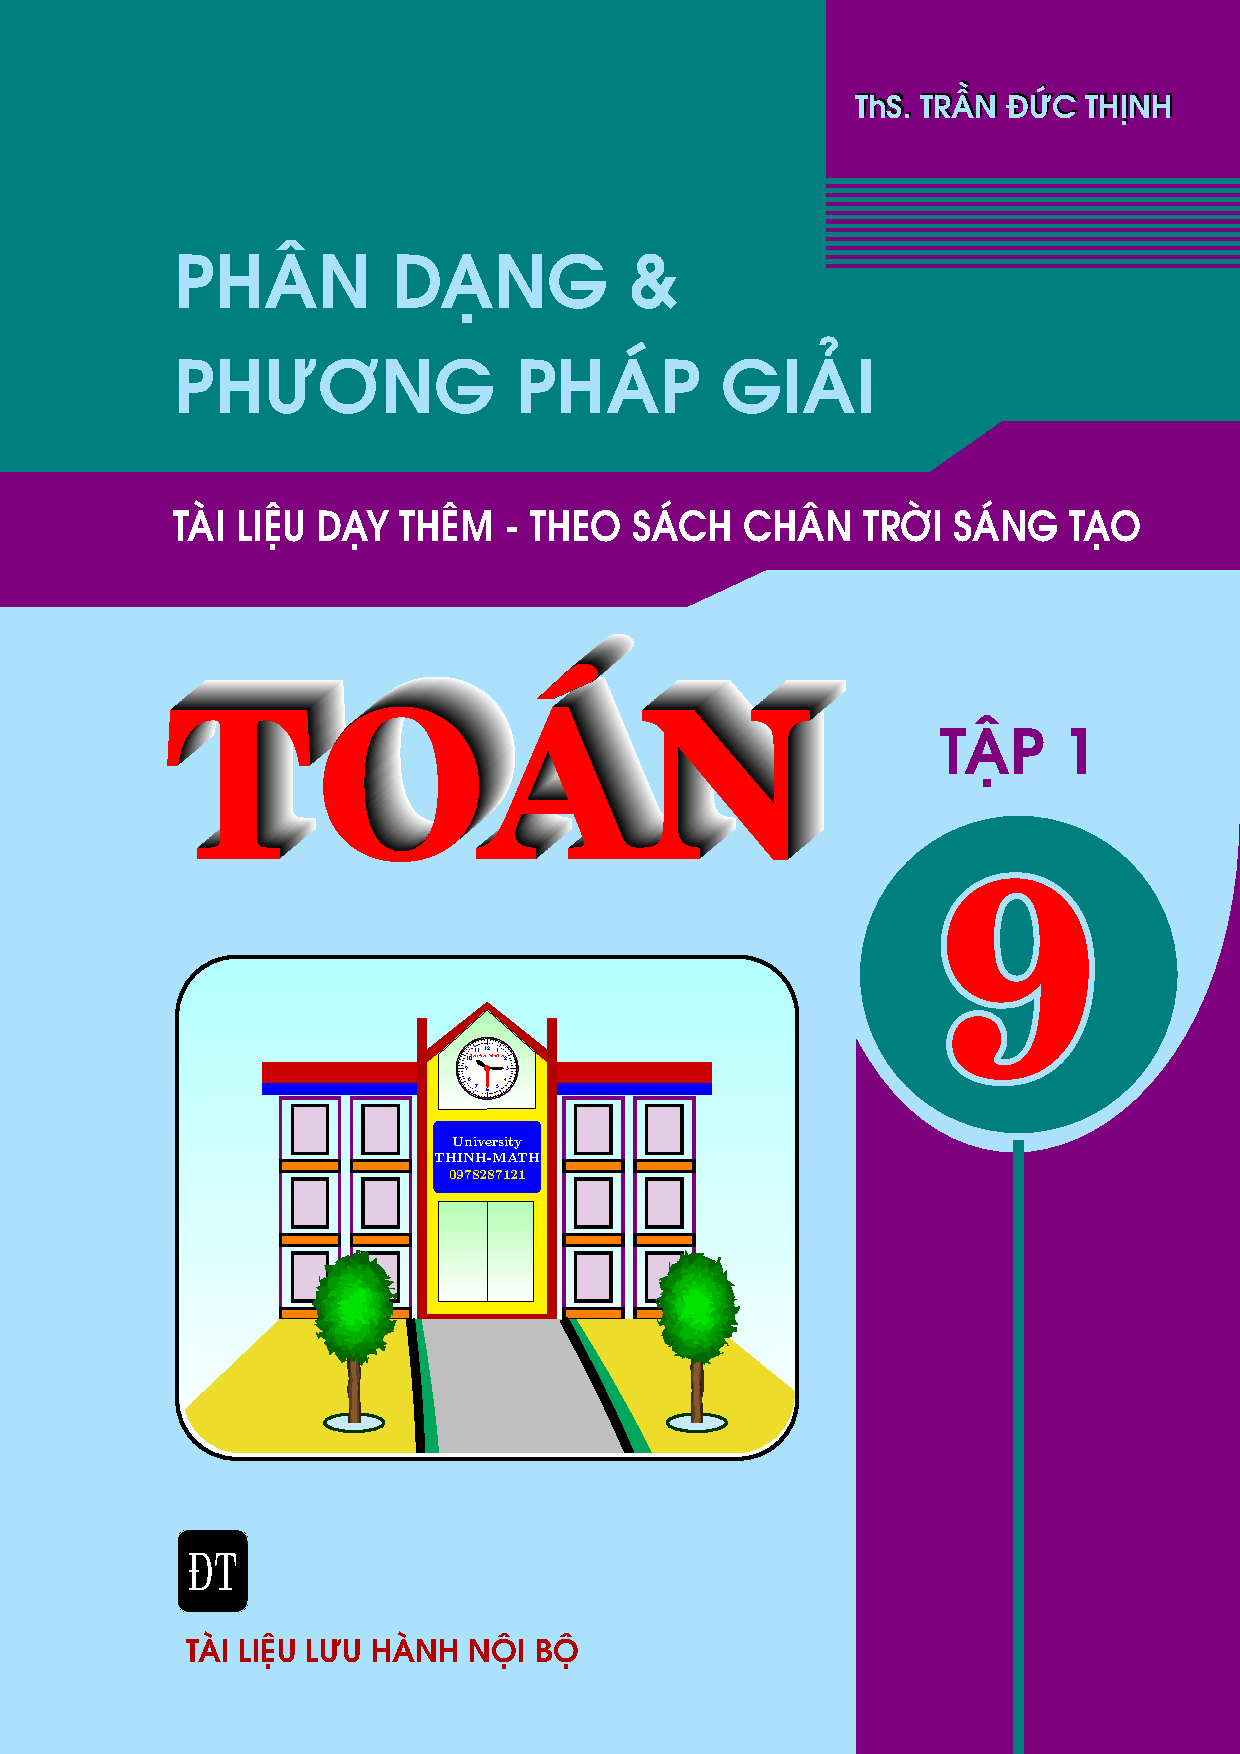
\includepdf{bia13/bia9-tap1-2.pdf}%chèn bìa pdf
%	\newpage\null\thispagestyle{empty}\newpage%tạo trang trống
	%--Mục lục chính
	\FULLWIDTH
	\muclucchinh
	%------------
	\clearpage%đặt lại đánh số trang
	\pagenumbering{arabic}%đánh số trang dạng 1,2,...
%====================================================
%==================BẮT ĐẦU TÀI LIỆU==================
%%%%\NOTE
%~~~~~~~~~~~~~~~~~~~~~~
\part{HỌC KÌ I}
%%%%%%%%%%%%%%%%%%% OKs
\setcounter{chapter}{0}  
\chapter{VẬT LÝ NHIỆT}
\setcounter{section}{0}
\section{SỰ CHUYỂN THỂ}
\subsection{LÝ THUYẾT TRỌNG TÂM}
\subsubsection{Mô hình động học phân tử về cấu tạo chất}
\begin{boxdn}
	Mô hình động học phân tử về cấu tạo chất có những nội dung cơ bản sau:
	\begin{enumerate}[label=\arabic*.]
		\item Các chất được cấu tạo từ các hạt riêng biệt gọi là phân tử.
		\item Các phân tử chuyển động hỗn loạn, không ngừng. Nhiệt độ của vật càng cao thì tốc độ chuyển động của các phân tử cấu tạo nên vật càng lớn.
		\item Giữa các phân tử có lực hút và đẩy gọi chung là lực liên kết phân tử.
	\end{enumerate}
\end{boxdn}
\subsubsection{Cấu trúc của chất rắn, lỏng, khí}
\paragraph{Phân biệt cấu trúc của chất rắn, lỏng, khí}
\begin{center}
	\begin{tabular}{|p{4cm}|p{4cm}|p{4cm}|p{4cm}|}
		\hline
		\rowcolor{\nenVD}
		\thead{Đặc điểm}&\thead{Thể rắn} &\thead{Thể lỏng}&\thead{Thể khí}\\
		\hline
		Khoảng cách giữa các phân tử & Rất gần nhau (cỡ kích thước phân tử) & Xa nhau & Rất xa nhau (gấp hàng chục lần kích thước phân tử)\\
		\hline
		Lực tương tác phân tử & Rất mạnh & Nhỏ hơn trong chất rắn & Rất yếu\\
		\hline
		Sự sắp xếp của các phân tử & Trật tự & Kém trật tự hơn & Không có trật tự\\
		\hline
		Chuyển động của các phân tử & Chỉ dao động quanh vị trí cân bằng cố định & Dao động quanh vị trí cân bằng luôn luôn thay đổi & Chuyển động hỗn loạn \\
		\hline
		Hình dạng & Hình dạng riêng xác định & Có hình dạng của bình chứa & Có hình dạng của bính chứa\\
		\hline
		Thể tích & Xác định & Xác định & Chiếm toàn bộ thể tích bình chứa\\
		\hline
	\end{tabular}
\end{center}
\paragraph{Chất rắn kết tinh và chất rắn vô định hình}
\begin{boxdn}
	\begin{itemize}
		\item \textbf{Chất rắn kết tinh} là chất mà các hạt (phân tử, nguyên tử, ion) cấu tạo nên nó ở thể rắn, liên kết với nhau một cách chặt chẽ, sắp xếp theo một trật tự hình học xác định tạo thành các mạng tinh thể.
	\end{itemize}
\end{boxdn}
\begin{boxvidu}
\textit{\textbf{Ví dụ:}} muối ăn, thạch anh, kim cương, nước đá, \dots
\end{boxvidu}
	
	\begin{center}
		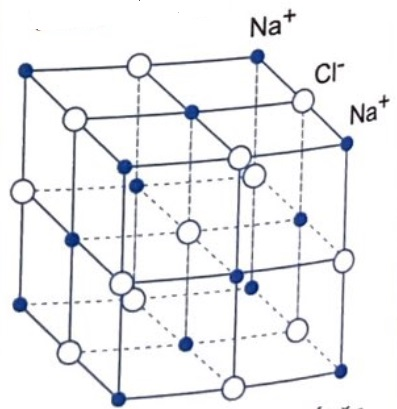
\includegraphics[width=0.2\linewidth]{figs/VN12-Y24-PH-SYL-001-3}
		\captionof{figure}{Cấu trúc tinh thể muối ăn}
	\end{center}
	\begin{boxdn}
		\begin{itemize}
		\item \textbf{Chất rắn vô định hình} là chất ở thể rắn mà các hạt tạo nên nó không tạo thành mạng tinh thể.\\
	\end{itemize}
	\end{boxdn}
\begin{boxvidu}
	\textbf{\textit{Ví dụ:}} thuỷ tinh, nhựa đường, sôcôla, \dots
\end{boxvidu}
\subsubsection{Sự chuyển thể}
\begin{boxdn}
	Khi các điều kiện như nhiệt độ, áp suất thay đổi, chất có thể chuyển từ thể này sang thể khác.
	\begin{itemize}
		\item Quá trình chuyển từ thể rắn sang thể lỏng của các chất được gọi là \textit{sự nóng chảy}. Quá trình ngược lại gọi là sự đông đặc.
		\item Quá trình chuyển từ thể lỏng sang thể khí (hơi) của các chất được gọi là \textit{sự hoá hơi}. Quá trình chuyển ngược lại gọi là sự ngưng tụ.
		\item Trong một số điều kiện, chất rắn có thể chuyển sang thể khí (hơi). Quá trình này gọi là sự thăng hoa. Quá trình ngược lại gọi là sự ngưng kết.\\
	\end{itemize}
\end{boxdn}
\begin{boxvidu}
	\textit{\textbf{Ví dụ:}} Sự thăng hoa dễ dàng của băng phiến ở nhiệt độ thường. Sự ngưng kết của hơi nước trong không khí tạo thành sương muối.
\end{boxvidu}
	\begin{center}
		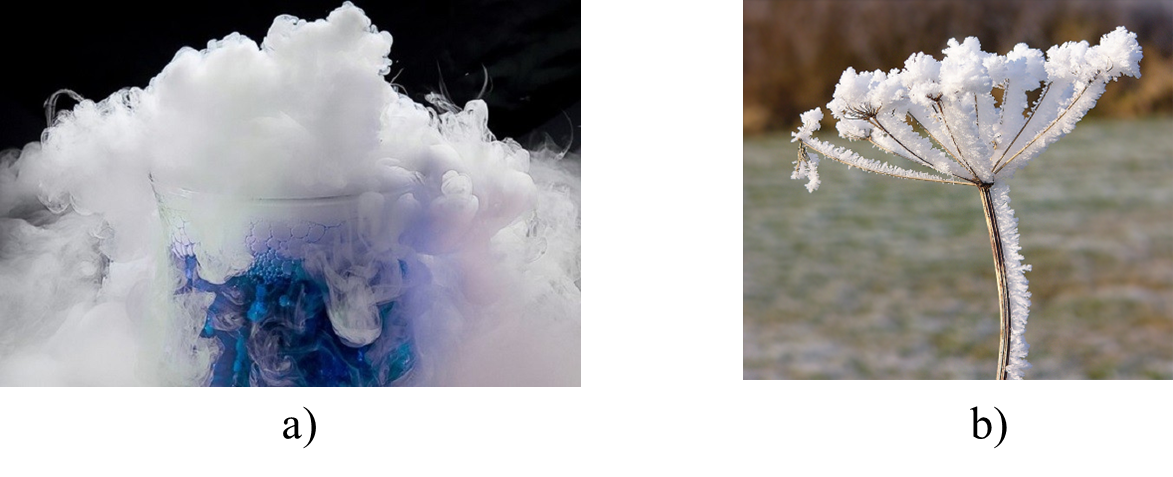
\includegraphics[width=0.7\linewidth]{figs/VN12-Y24-PH-SYL-001-7}
		\captionof{figure}{a) Đá khô thăng hoa; b) Sương muối}
	\end{center}

\begin{center}
	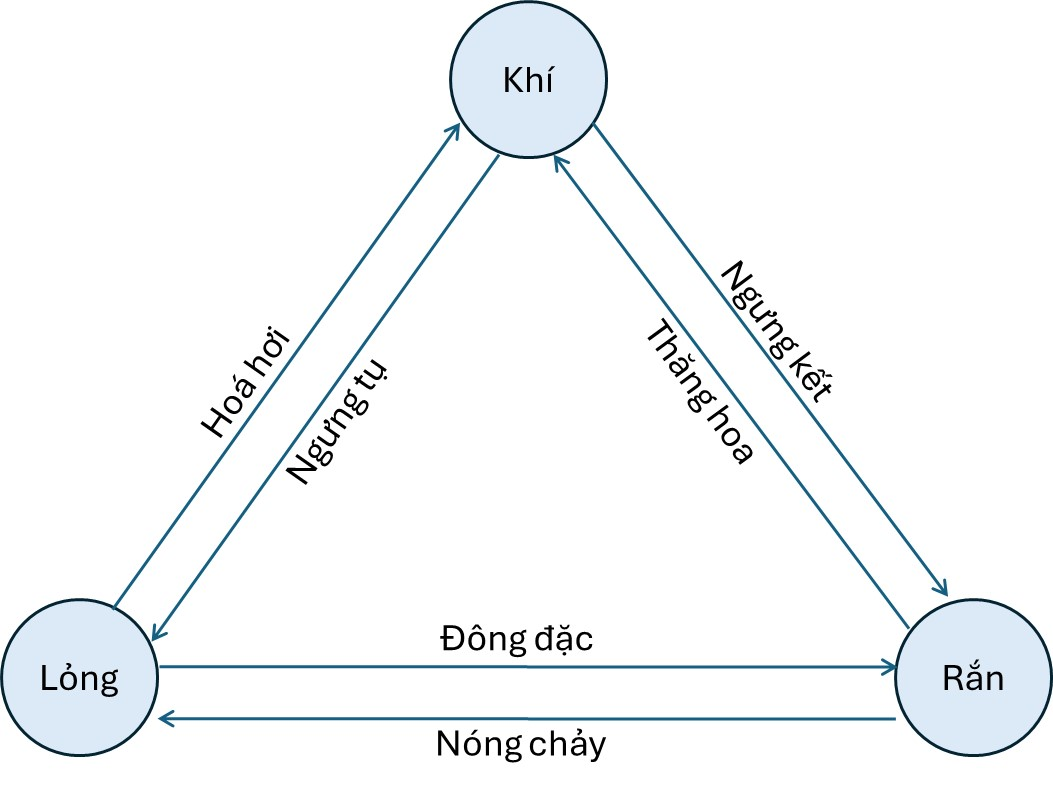
\includegraphics[width=0.5\linewidth]{figs/VN12-Y24-PH-SYL-001-4}
	\captionof{figure}{Sơ đồ các hình thức chuyển thể}
\end{center}
\paragraph{Sự nóng chảy}
\begin{boxdn}
	Khi đun nóng đến một nhiệt độ nào đó, vật rắn bắt đầu chuyển trạng thái từ rắn sang lỏng (sự nóng chảy). Chất rắn kết tinh có nhiệt độ nóng chảy xác định (ở một áp suất cụ thể). Chất rắn vô định hình không có nhiệt độ nóng chảy xác định.\\
\end{boxdn}
\begin{boxvidu}
	\textbf{\textit{Ví dụ:}}
	\begin{itemize}
		\item Khi nung nóng nước đá ở áp suất tiêu chuẩn, nhiệt độ nước đá tăng dần. Khi đạt đến $\SI{0}{\celsius}$, nước đá bắt đầu tan và trong suốt quá trình hoá lỏng nhiệt độ của nước đá không đổi. Nước đá là chất rắn kết tinh.
		\item Khi nung nóng thỏi sôcôla, thỏi sôcôla mềm đi và chuyển dần sang thể lỏng, trong quá trình này nhiệt độ của thỏi sôcôla vẫn tăng liên tục. Thỏi sôcôla là chất rắn vô định hình.
	\end{itemize}
	\begin{center}
		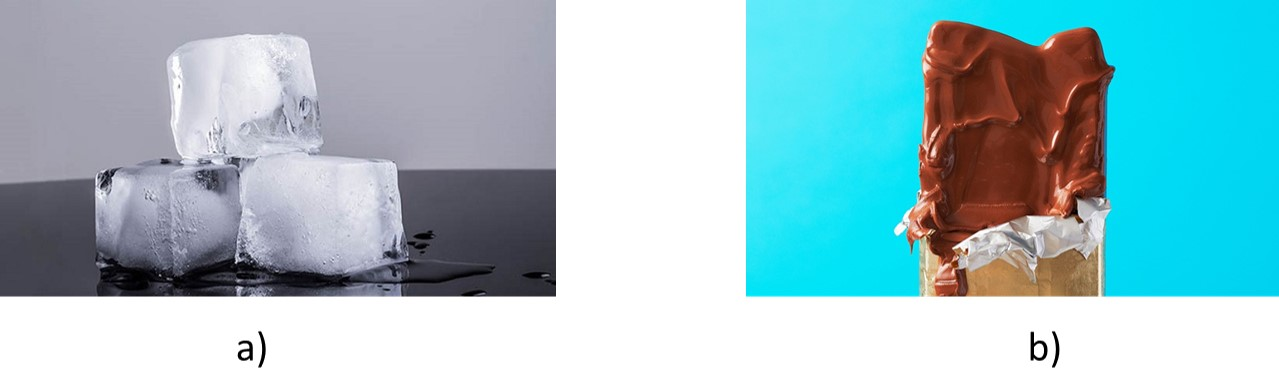
\includegraphics[width=0.6\linewidth]{figs/VN12-Y24-PH-SYL-001-5}
		\captionof{figure}{a) Nước đá đang tan; b) Thanh sôcôla đang nóng chảy}
	\end{center}
\end{boxvidu}
\paragraph{Sự hoá hơi}
\begin{boxdn}
	\begin{itemize}
		\item \textbf{Sự bay hơi}\\
		Sự bay hơi là sự hoá hơi xảy ra \textbf{trên bề mặt chất lỏng}. Sự bay hơi xảy ra ở \textbf{nhiệt độ bất kì}.\\
		Tốc độ bay hơi của chất lỏng càng nhanh nếu diện tích mặt thoáng càng lớn, tốc độ gió càng lớn, nhiệt độ càng cao, và độ ẩm không khí càng thấp.
		\item \textbf{Sự sôi}\\
		Sự sôi là sự hoá hơi xảy ra \textbf{bên trong và trên bề mặt chất lỏng}. Sự sôi xảy ra ở \textbf{nhiệt độ sôi}.\\
		Nhiệt độ sôi của chất lỏng phụ thuộc áp suất khí trên mặt thoáng và bản chất của chất lỏng. Trong suốt thời gian sôi, nhiệt độ của chất lỏng không thay đổi.
	\end{itemize}
\end{boxdn}
\begin{center}
	
	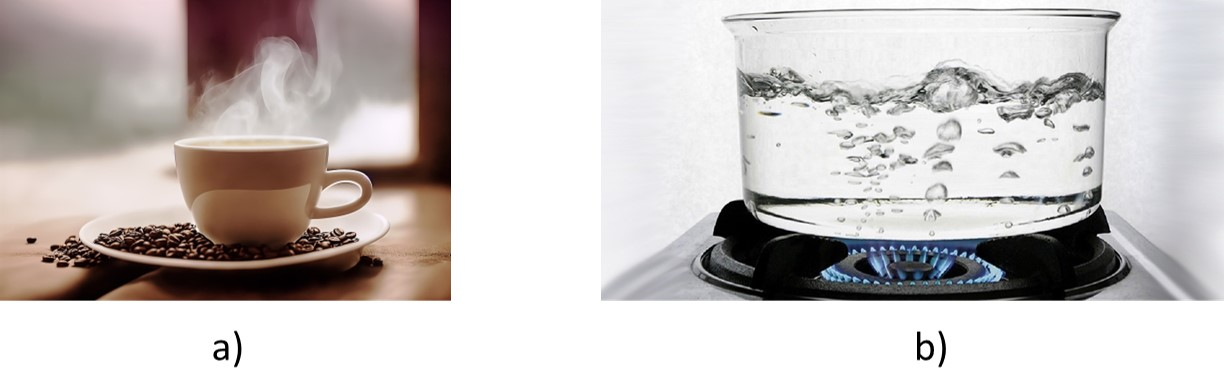
\includegraphics[width=0.65\linewidth]{figs/VN12-Y24-PH-SYL-001-6}
	\captionof{figure}{a) Nước bay hơi trên mặt thoáng của tách cà phê; b) Nước đang sôi}
\end{center}
\subsection{VÍ DỤ MINH HOẠ}
\begin{dang}{Sử dụng mô hình động học phân tử, nêu được sơ lược cấu trúc của chất rắn, chất lỏng, chất khí}
\end{dang}
\begin{vd}
	Năm 1827, khi làm thí nghiệm quan sát các hạt phấn hoa rất nhỏ trong nước bằng kính hiển vi, Brown thấy chúng chuyển động hỗn loạn, không ngừng. Chuyển động này được gọi là chuyển động Brown.\\
	\begin{center}
		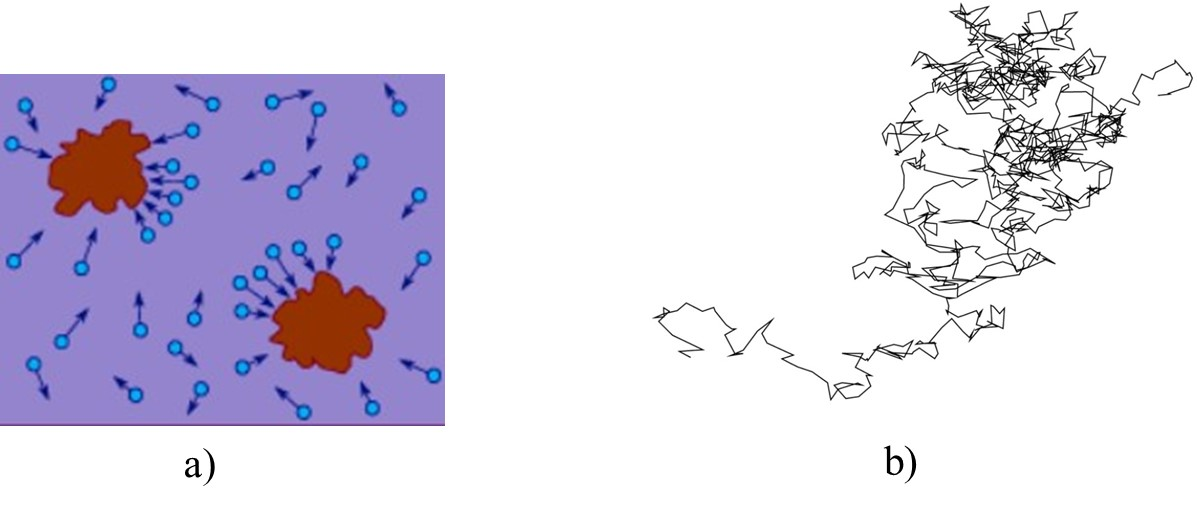
\includegraphics[width=0.6\linewidth]{figs/VN12-Y24-PH-SYL-001-1}
		\captionof{figure}{a) Mô phỏng sự va chạm giữa các phân tử nước với các hạt phấn hoa; b) Quỹ đạo chuyển động của hạt phấn hoa}
	\end{center}
	\begin{enumerate}[label=\alph*)]
		\item Tại sao thí nghiệm của Brown được gọi là một trong những thí nghiệm chứng tỏ các phân tử chuyển động hỗn loạn không ngừng?
		\item Làm thế nào để với thí nghiệm của Brown có thể chứng tỏ được khi nhiệt độ của nước càng cao thì các phân tử nước chuyển động càng nhanh?
	\end{enumerate}
	\loigiai{
		\begin{enumerate}[label=\alph*)]
			\item Thông qua việc quan sát hạt phấn hoa trong nước, Brown nhận thấy rằng các hạt phấn hoa lắc lư không ngừng và quỹ đạo chuyển động của hạt phấn hoa hỗn loạn. Mà chuyển động của hạt phấn hoa là do sự va chạm  giữa các phân tử nước với hạt phấn hoa gây ra. Điều này chứng tỏ rằng chuyển động của các phân tử nước cũng hỗn loạn, không ngừng.
			\item Để với thí nghiệm của Brown có thể chứng tỏ được khi nhiệt độ của nước càng cao thì các phân tử nước chuyển động càng nhanh thì chúng ta có thể đun nóng nước rồi quan sát sự thay đổi tốc độ chuyển động của hạt phấn hoa.
	\end{enumerate}}
\end{vd}
\begin{vd}
	Hãy giải thích đặc điểm sau đây của thể khí, thể rắn, thể lỏng.
	\begin{enumerate}[label=\alph*)]
		\item Chất khí không có hình dạng và thể tích riêng, luôn chiếm toàn bộ thể tích bình chứa và có thể nén được dễ dàng.
		\item Vật ở thể rắn có thể tích và hình dạng riêng, rất khó nén.
		\item Vật ở thể lỏng có thể tích riêng nhưng không có hình dạng riêng.
	\end{enumerate}
	\loigiai{
		\begin{enumerate}[label=\alph*)]
			\item Ở thể khí, các phân tử ở xa nhau (khoảng cách giữa các phân tử lớn gấp hàng chục lần kích thước phân tử). Lực tương tác giữa các phân tử rất yếu (trừ trường hợp chúng va chạm nhau) nên các phân tử chuyển động hoàn toàn hỗn loạn. Do đó, khối chất khí không có hình dạng và thể tích riêng mà có hình dạng và thể tích của bình chứa nó.
			\item Ở thể rắn, các phân tử rất gần nhau (khoảng cách giữa các phân tử cỡ kích thước phân tử) và các phân tử sắp xếp có trật tự, chặt chẽ. Lực tương tác giữa các phân tử rất mạnh, giữ cho chúng không di chuyển tự do mà chỉ có thể dao động quanh vị trí cân bằng xác định. Do đó, vật rắn luôn có thể tích và hình dạng riêng xác định, đồng thời rất khó nén.
			\item Khoảng cách giữa các phân tử trong chất lỏng lớn hơn khoảng cách giữa các phân tử trong chất rắn và nhỏ hơn khoảng cách giữa các phân tử trong chất khí. Lực tương tác giữa các phân tử ở thể lỏng lớn hơn lực tương tác giữa các phân tử ở thể khí nên giữ các phân tử không bị phân tán ra xa nhau, do đó chất lỏng có thể tích riêng xác định. Lực tương tác này chưa đủ lớn như trong thể rắn nên các phân tử ở thể lỏng cũng dao động quanh vị trí cân bằng nhưng các vị trí cân bằng này luôn luôn thay đổi. Do đó, khối chất lỏng không có hình dạng riêng xác định mà có hình dạng của bình chứa nó.
	\end{enumerate}}
\end{vd}

\begin{dang}{Giải thích được sơ lược một số hiện tượng vật lí liên quan đến sự chuyển thể: sự nóng chảy, sự hoá hơi}
\end{dang}
%\setcounter{vd}{0}
\begin{vd}
	Vận dụng mô hình động học phân tử, em hãy giải thích nguyên nhân gây ra sự nóng chảy của chất rắn kết tinh.
	\loigiai{
		Ở áp suất không đổi, các phân tử ở thể rắn liên kết chặt chẽ với nhau, chúng dao động quanh các vị trí cân bằng xác định. Khi nung nóng chất rắn kết tinh, các phân tử được cung cấp nhiệt năng làm tốc độ chuyển động nhiệt của nó tăng lên, mức độ trật tự trong cấu trúc của các hạt giảm đi.  Điều này dẫn đến khoảng cách trung bình giữa các phân tử tăng.\\
		Nhiệt độ của vật rắn tăng đến một giá trị nào đó thì một số phân tử thắng được lực liên kết với các phân tử xung quanh và thoát khỏi liên kết với chúng, đó là sự khởi đầu của quá trình nóng chảy. Từ lúc này, vật rắn nhận nhiệt lượng để tiếp tục phá vỡ các liên kết tinh thể. Khi trật tự của tinh thể bị phá vỡ hoàn toàn thì quá trình nóng chảy kết thúc, vật rắn chuyển thành khối chất lỏng.
	}
\end{vd}
\begin{vd}
	Vận dụng mô hình động học phân tử, em hãy giải tích nguyên nhân gây ra sự bay hơi và sự sôi.

\loigiai{\begin{itemize}
		\item \textbf{Giải thích sự bay hơi:}\\
		Các phân tử ở bề mặt chất lỏng tham gia chuyển động nhiệt, trong đó có những phân tử chuyển động hướng ra ngoài chất lỏng. Đồng thời, các phân tử có thể truyền năng lượng cho nhau thông qua quá trình va chạm. Do đó, một số phân tử ở gần mặt thoáng của chất lỏng có động năng đủ lớn để thắng lực liên kết của các phân tử chất lỏng khác thì thoát được ra khỏi mặt thoáng của chất lỏng trở thành các phân tử ở thể hơi.
		\item \textbf{Giải thích sự sôi:}\\
		Khi chất lỏng đến nhiệt độ sôi, do tiếp tục được cung cấp nhiệt nên các phân tử chất lỏng chuyển động nhiệt mạnh hơn, làm phá vỡ sự liên kết giữa các phân tử chất lỏng với nhau. Khi đó các bọt chứa không khí và hơi nước nổi lên trong lòng nước càng ngày càng nhiều, càng nổi lên trên thể tích các bọt khí này càng tăng, tới mặt thoáng thì vỡ, không khí và hơi nước thoát ra ngoài khí quyển.
\end{itemize}}
\end{vd}


\subsection{BÀI TẬP TRẮC NGHIỆM}

\Opensolutionfile{ans}[ans/G12Y24B1TN]
\begin{ex}
Chuyển động của các nguyên tử, phân tử trong mô hình động học phân tử được gọi là chuyển động
\choice
{chuyển động cơ}
{\True chuyển động nhiệt}
{chuyển động tròn}
{chuyển động đều}
\loigiai{ }
\end{ex}

%==============================================
\begin{ex}

Chọn phát biểu \textbf{đúng} về lực tương tác giữa các phân tử.
\choice
{\True Giữa các phân tử có cả lực hút và lực đẩy}
{ Giữa các phân tử chỉ có lực hút hoặc lực đẩy}
{ Giữa các phân tử chỉ có lực đẩy}
{ Giữa các phân tử chỉ có lực hút}
\loigiai{ }
\end{ex}

%==============================================
\begin{ex}
Khi khoảng cách giữa các phân tử rất nhỏ, thì giữa các phân tử
\choice
{ chỉ có lực hút}
{ chỉ có lực đẩy}
{\True có cả lực hút và lực đẩy, nhưng lực đẩy lớn hơn lực hút}
{ có cả lực hút và lực đẩy, nhưng lực đẩy nhỏ hơn lực hút}
\loigiai{ }
\end{ex}


%==============================================
\begin{ex}
Mục đích của thí nghiệm Brown là
\choice
{ quan sát hạt phấn hoa bằng kính hiển vi}
{\True quan sát chuyển động của hạt phấn hoa trong nước bằng kính hiển vi}
{ quan sát cánh hoa trong nước bằng kính hiển vi}
{ quan sát chuyển động của cánh hoa}
\loigiai{ }
\end{ex}


%==============================================
\begin{ex} 
Trong thí nghiệm của Brown các hạt phấn hoa chuyển động hỗn độn, không ngừng vì
\choice
{ giữa các hạt phấn hoa có lực tương tác hút và đẩy}
{ các hạt phấn hoa là các thực thể sống}
{\True các phân tử nước chuyển động không ngừng, va chạm vào chúng từ mọi phía}
{ các hạt phấn hoa có thể dao động tự do quanh vị trí cân bằng}
\loigiai{ }
\end{ex}


%==============================================
\begin{ex}
Chọn câu trả lời \textbf{đúng nhất}. \\
Các chất có thể tồn tại ở những thể nào?
\choice
{ Thể rắn, thể lỏng, thể khí hoặc chân không}
{\True Thể rắn, thể lỏng hoặc thể khí}
{ Thể rắn và thể hơi}
{ Thể rắn và thế lỏng}
\loigiai{ }
\end{ex}


%==============================================
\begin{ex}
Đặc điểm nào sau đây là phù hợp với chất rắn?
\choice
{\True Có lực tương tác giữa các phân tử rất mạnh}
{ Có lực tương tác giữa các phân tử rất yếu}
{ Không có hình dạng xác định}
{ Không có thể tích riêng xác định}
\loigiai{ }
\end{ex}


%==============================================
\begin{ex}
Phát biểu nào dưới đây là đúng khi nói về những đặc điểm của chất rắn?
\choice
{ Có khối lượng, hình dạng xác định, không có thể tích xác định}
{ Có khối lượng xác định, hình dạng và thể tích không xác định}
{\True Có khối lượng, hình dạng, thể tích xác định}
{ Có khối lượng và thể tích xác định, hình dạng không xác định}
\loigiai{ }
\end{ex}


%==============================================
\begin{ex}
Người ta có thể phân loại chất rắn một cách tổng quát theo cách nào sau đây?
\choice
{ Chất rắn đơn tinh thể và chất rắn vô định hình}
{\True Chất rắn kết tinh và chất rắn vô định hình}
{ Chất rắn đa tinh thể và chất rắn vô định hình}
{ Chất rắn đơn tinh thể và chất rắn đa tinh thể}
\loigiai{ }
\end{ex}


%==============================================
\begin{ex} 
Đặc điểm nào sau đây là đặc điểm cấu trúc phân tử ở thể lỏng?
\choice
{ Khoảng cách giữa các phân tử rất lớn so với kích thước của chúng}
{\True Lực tương tác phân tử yếu hơn lực tương tác phân tử ở thể rắn}
{ Không có thể tích và hình dạng riêng xác định}
{ Các phân tử dao động xung quanh vị trí cân bằng xác định}
\loigiai{ }
\end{ex}


%==============================================
\begin{ex} 
Trong chuyển động nhiệt, các phân tử chất lỏng
\choice
{ dao động quanh vị trí cân bằng xác định}
{ chuyển động hỗn loạn quanh vị trí cân bằng xác định}
{ chuyển động hỗn loạn}
{\True dao động quanh vị trí cân bằng nhưng những vị trí này không cố định mà luôn thay đổi}
\loigiai{ }
\end{ex}


%==============================================
\begin{ex}
Chất lỏng có thể tích xác định, nhưng hình dạng không xác định là do trong chất lỏng
\choice
{ lực liên kết giữa các phân tử chất lỏng là rất lớn, các phân tử chỉ dao động không ngừng quanh một vị trí xác định}
{ lực liên kết giữa các phân tử chất lỏng là rất yếu, các phân tử dao động tự do về mọi phía}
{\True lực liên kết giữa các phân tử chất lỏng là yếu hơn chất rắn, các phân tử dao động tương đối tự do hơn so với trong chất rắn}
{ Tất cả các phương án đưa ra đều sai}
\loigiai{ }
\end{ex}


%==============================================
\begin{ex} 
Các phân tử khí chuyển động hỗn loạn, không ngừng vì
\choice
{ phân tử khí không có khối lượng}
{ khoảng cách giữa các phân tử khí quá gần nhau}
{\True lực tương tác giữa các phân tử quá nhỏ}
{ các phân tử khí luôn đẩy nhau}
\loigiai{ }
\end{ex}


%==============================================
\begin{ex}
Tính chất nào sau đây \textbf{không phải} là tính chất của chất ở thể khí?
\choice
{\True Có hình dạng và thể tích riêng}
{ Có các phân tử chuyển động hoàn toàn hỗn độn}
{ Có thể nén được dễ dàng}
{ Có lực tương tác phân tử nhỏ hơn lực tương tác phân tử ở thể rắn và thể lỏng}
\loigiai{ }
\end{ex}


%==============================================
\begin{ex}
Chất khí không có hình dạng và thể tích riêng là vì
\choice
{ khoảng cách giữa các phân tử rất gần, lực tương tác giữa các phân tử chất khí rất mạnh}
{ khoảng cách giữa các phân tử rất gần, lực tương tác giữa các phân tử chất khí rất yếu}
{ khoảng cách giữa các phân tử rất xa, lực tương tác giữa các phân tử chất khí rất mạnh}
{\True khoảng cách giữa các phân tử rất xa, lực tương tác giữa các phân tử chất khí rất yếu}
\loigiai{ }
\end{ex}


%==============================================
\begin{ex}
Khi mở nắp lọ nước hoa, ta có thể ngửi thấy mùi thơm tràn ngập trong phòng. Điều này thể hiện tính chất nào của chất khí?
\choice
{ Dễ dàng nén được}
{ Có khối lượng xác định}
{\True Có thể khuếch tán trong không gian theo mọi hướng}
{ Không chảy được}
\loigiai{ }
\end{ex}


%==============================================
\begin{ex}
Sự nóng chảy là
\choice
{\True sự chuyển thế từ rắn sang lỏng}
{ sự chuyển thể từ rắn sang khí}
{ sự chuyển thể từ lỏng sang rắn}
{ sự chuyển thể từ lỏng sang khí}
\loigiai{ }
\end{ex}


%==============================================
\begin{ex}
Sự đông đặc là
\choice
{ sự chuyển thế từ rắn sang lỏng}
{ sự chuyển thể từ rắn sang khí}
{\True sự chuyển thể từ lỏng sang rắn}
{ sự chuyển thể từ lỏng sang khí}
\loigiai{ }
\end{ex}
%==============================================
\begin{ex}
Sự bay hơi là
\choice
{ sự chuyển thế từ rắn sang lỏng}
{ sự chuyển thể từ rắn sang khí}
{ sự chuyển thể từ lỏng sang rắn}
{\True sự chuyển thể từ lỏng sang khí}
\loigiai{ }
\end{ex}
%==============================================
\begin{ex}
Khi quan sát sự nóng chảy của nước đá, trong suốt thời gian nóng chảy thì
\choice
{ nhiệt độ của nước đá tăng}
{ nhiệt độ của nước đá giảm}
{\True nhiệt  độ của nước đá không đổi}
{ nhiệt độ của nước đá ban đầu tăng và sau đó giảm}
\loigiai{ }
\end{ex}
%==============================================
\begin{ex}
Phát biểu nào sau đây về tính chất của chất rắn kết tinh và chất rắn vô định hình là \textbf{đúng}?
\choice
{ Chất rắn kết tinh và chất rắn vô định hình đều có nhiệt độ nóng chảy xác định}
{ Chất rắn kết tinh không có nhiệt độ nóng chảy xác định, chất rắn vô định hình có nhiệt độ nóng chảy xác định}
{\True Chất rắn kết tinh có nhiệt độ nóng chảy xác định, chất rắn vô định hình không có nhiệt độ nóng chảy xác định}
{ Chất rắn kết tinh và chất rắn vô định hình đều không có nhiệt độ nóng chảy xác định}
\loigiai{ }
\end{ex}
%==============================================
\begin{ex}
Một vật rắn khi bị nung nóng thì mềm dần. Đó là
\choice
{ chất rắn kết tinh}
{ chất rắn đơn tinh thể}
{ chất rắn đa tinh thể}
{\True chất rắn vô định hình}
\loigiai{ }
\end{ex}
%==============================================
\begin{ex}
Trường hợp nào sau đây không liên quan đến sự nóng chảy và đông đặc?
	\begin{center}
		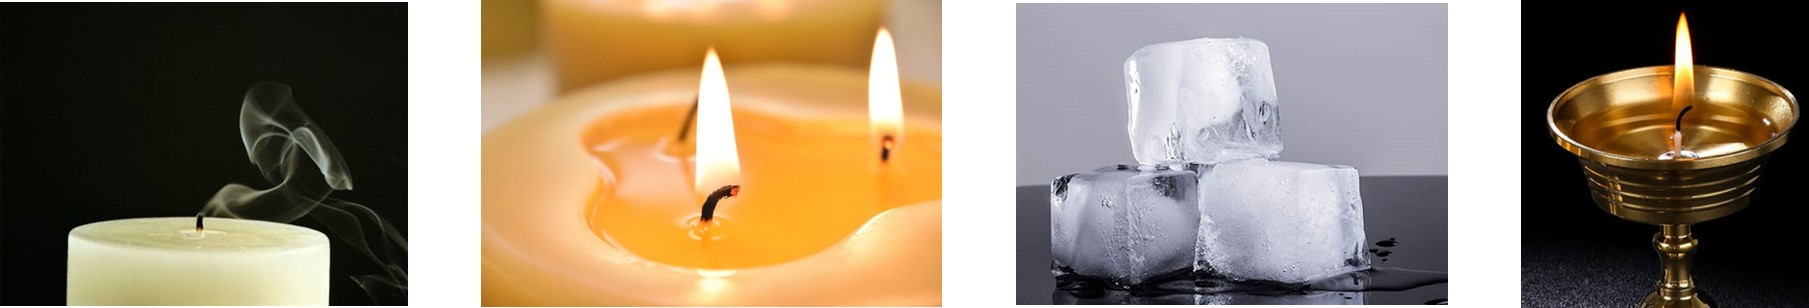
\includegraphics[width=0.45\linewidth]{figs/VN12-Y24-PH-SYL-001P-2}
	\end{center}
\choice
{ Ngọn nến vừa tắt}
{ Ngọn nến đang cháy}
{ Nước đá vừa lấy ra khỏi tủ lạnh}
{\True Ngọn đèn dầu đang cháy}
\loigiai{ }
\end{ex}
%==============================================
\begin{ex}
Sự bay hơi diễn ra càng nhanh hơn khi
\choice
{ nhiệt độ càng thấp}
{\True tốc độ gió càng lớn}
{ lượng chất lỏng càng nhiều}
{ diện tích mặt thoáng càng hẹp}
\loigiai{ }
\end{ex}
%==============================================
\begin{ex}
Một ấm nước đang sôi, nếu tiếp tục đun thì
\choice
{ nhiệt độ nước trong ấm giảm xuống}
{ nước trong ấm không bay hơi nữa}
{ nhiệt độ nước trong ấm vẫn tiếp tục tăng}
{\True nước trong ấm bay hơi nhiều hơn và cạn dần}
\loigiai{ }
\end{ex}
%==============================================
\begin{ex}
Phát biểu nào sau đây là \textbf{không đúng} về sự bay hơi?
\choice
{ Sự bay hơi là quá trình chuyển từ thể lỏng sang thể khí xảy ra ở bề mặt chất lỏng}
{\True Sự bay hơi là quá trình chuyển từ thể lỏng sang thể khí xảy ra ở cả bên trong và trên bề mặt chất lỏng}
{ Sự bay hơi của chất lỏng xảy ra ở nhiệt độ bất kì}
{ Sự ngưng tụ luôn kèm theo sự bay hơi}
\loigiai{ }
\end{ex}
%==============================================
\begin{ex}
Sự sôi xảy ra ở
\choice
{ nhiệt độ trên $\SI{100}{\celsius}$}
{ $\SI{100}{\celsius}$}
{\True nhiệt độ sôi}
{ dưới $\SI{100}{\celsius}$}
\loigiai{ }
\end{ex}
%==============================================
\begin{ex}
Trong các trường hợp dưới đây, trường hợp nào liên quan đến sự bay hơi?
\choice
{ Kính cửa sổ bị mờ đi trong những ngày đông giá lạnh}
{\True Dầu trong đèn bị khô cạn dù không sử dụng}
{ Miếng bơ để bên ngoài tủ lạnh sau một thời gian bị chảy lỏng}
{ Đưa nước vào trong tủ lạnh để làm đá}
\loigiai{ }
\end{ex}
%==============================================
\begin{ex}
Tại sao quả bóng bay dù buộc chặt để lâu ngày vẫn bị xẹp?
\choice
{ Vì khi mới thổi, không khí từ miệng vào bóng còn nóng, sau đó lạnh dần nên co lại}
{ Vì cao su là chất đàn hồi nên sau khi bị thổi căng nó tự động co lại}
{ Vì không khí nhẹ nên có thể chui qua chỗ buộc ra ngoài}
{\True Vì giữa các phân tử của chất làm vỏ bóng có khoảng cách nên các phân tử không khí có thể chui qua đó và thoát ra ngoài}
\loigiai{ }
\end{ex}
%==============================================
\begin{ex}
Hãy chọn phương án \textbf{sai}.\\
Cùng một khối lượng của một chất nhưng khi ở các thể khác nhau thì sẽ khác nhau
\choice
{ Thể tích}
{ Khối lượng riêng}
{\True Kích thước của các nguyên tử}
{ Trật tự của các nguyên tử}
\loigiai{ }
\end{ex}
%==============================================
\begin{ex}
Các nguyên tử trong một miếng sắt có tính chất nào sau đây?
\choice
{ Khi nhiệt độ tăng thì nở ra}
{ Khi nhiệt độ giảm thì co lại}
{\True Đứng rất gần nhau}
{ Đứng xa nhau}
\loigiai{ }
\end{ex}
%==============================================
\begin{ex}
Trong các chất sau, chất nào \textbf{không phải} là chất rắn kết tinh?
\choice
{ Muối ăn}
{\True Thuỷ tinh}
{ Kim cương}
{ Thạch anh}
\loigiai{ }
\end{ex}
%==============================================
\begin{ex}
Chất rắn nào dưới đây không phải là chất rắn vô định hình?
\choice
{\True Thạch anh}
{ Thuỷ tinh}
{ Sáp}
{ Cao su}
\loigiai{ }
\end{ex}
%==============================================
\begin{ex}
Chất rắn nào dưới đây là chất rắn vô định hình?
\choice
{ Muối ăn}
{ Kim loại}
{ Thạch anh}
{\True Nhựa đường}
\loigiai{ }
\end{ex}
%==============================================
\begin{ex}
Ở điều kiện thường, iode là chất rắn dạng tinh thể màu đen tím. Khi đun nóng, iode có sự thăng hoa.\\
Vậy sự thăng hoa của iode là sự chuyển trạng thái từ thể
\choice
{\True rắn sang khí}
{ rắn sang lỏng}
{ lỏng sang rắn}
{ khí sang rắn}
\loigiai{ }
\end{ex}
%==============================================
\begin{ex}
Cho đồ thị biểu diễn sự thay đổi nhiệt độ theo thời gian của nước đá như hình vẽ. Nước đá tan trong khoảng thời gian nào?
\begin{center}
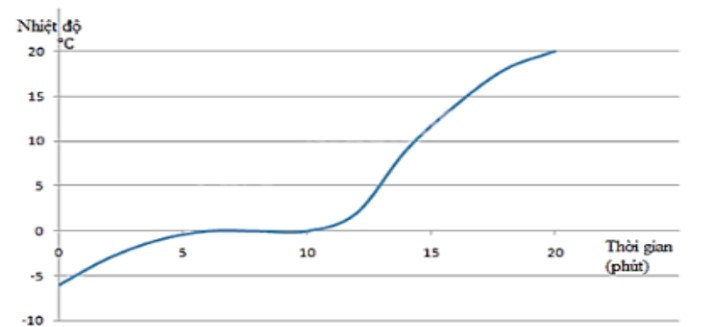
\includegraphics[width=0.6\linewidth]{figs/VN12-Y24-PH-SYL-001P-1}
\end{center}
\choice
{\True Từ phút thứ 6 đến phút thứ 10}
{ Từ phút thứ 10 trở đi}
{ Từ 0 đến phút thứ 6}
{ Từ phút thứ 10 đến phút thứ 15}
\loigiai{ }
\end{ex}
%==============================================
\begin{ex}
Người ta không thể luộc trứng chín ở núi cao vì
\choice
{\True áp suất trên núi thấp hơn áp suất chuẩn $\left(\SI{1}{atm}\right)$ nên nước sôi ở nhiệt độ thấp hơn $\SI{100}{\celsius}$}
{ áp suất trên núi cao hơn áp suất chuẩn $\left(\SI{1}{atm}\right)$ nên nước sôi ở nhiệt độ thấp hơn $\SI{100}{\celsius}$}
{ áp suất trên núi thấp hơn áp suất chuẩn $\left(\SI{1}{atm}\right)$ nên nước sôi ở nhiệt độ cao hơn $\SI{100}{\celsius}$}
{ áp suất trên núi cao hơn áp suất chuẩn $\left(\SI{1}{atm}\right)$ nên nước sôi ở nhiệt độ cao hơn $\SI{100}{\celsius}$}
\loigiai{ }
\end{ex}
%==============================================
\begin{ex}
Thuỷ ngân có nhiệt độ nóng chảy là $\SI{-39}{\celsius}$ và nhiệt độ sôi là $\SI{357}{\celsius}$. Khi ở trong phòng có nhiệt độ $\SI{30}{\celsius}$ thì thuỷ ngân
\choice
{\True chỉ tồn tại ở thể lỏng}
{ chỉ tồn tại ở thể hơi}
{ tồn tại ở cả thể lỏng và thể hơi}
{ tồn tại ở cả thể rắn, lỏng và hơi}
\loigiai{ }
\end{ex}
%==============================================
\begin{ex}
Tại sao khi cầm vào vỏ bình ga mini đang sử dụng ta thường thấy có một lớp nước rất
mỏng trên đó?
\choice
{ Do hơi nước từ tay ta bốc ra}
{ Nước từ trong bình ga thấm ra}
{\True Do vỏ bình ga lạnh hơn nhiệt độ môi trường nên hơi nước trong không khí ngưng tụ trên đó}
{ Cả B và C đều đúng}
\loigiai{ }
\end{ex}
%==============================================
\begin{ex}
Ở nhiệt độ trong phòng, chỉ có thể có khí oxygen, không thể có oxygen lỏng vì
\choice
{ oxygen luôn là chất khí}
{\True nhiệt độ phòng cao hơn nhiệt độ sôi của oxygen}
{ nhiệt độ phòng thấp hơn nhiệt độ sôi của oxygen}
{ nhiệt độ trong phòng bằng nhiệt độ sôi của oxygen}
\loigiai{ }
\end{ex}

\Closesolutionfile{ans}

\subsection{TRẮC NGHIỆM ĐÚNG/SAI}
\Opensolutionfile{ans}[ans/G12Y24B1DS]
\setcounter{ex}{0}
\begin{ex}
	Nhận định các phát biểu sau đây về mô hình động học phân tử.
	\begin{enumerate}[label=\alph*)]
		\item Các chất được cấu tạo từ các hạt riêng biệt được gọi nguyên tử, phân tử.
		\item Các nguyên tử, phân tử đứng sát nhau và giữa chúng không có khoảng cách.
		\item Lực tương tác giữa các phân tử ở thể rắn lớn hơn lực tương tác giữa các phân tử ở thể lỏng và thể khí.
		\item Các nguyên tử, phân tử chất lỏng dao động xung quanh các vị trí cân bằng không cố định.
	\end{enumerate}
\loigiai{
\begin{enumerate}[label=\alph*)]
	\item Đúng.
	\item Sai.
	\item Đúng.
	\item Đúng.
\end{enumerate}
}
	\end{ex}
%=====================================================================================
\begin{ex}
	Nhận định các phát biểu về sự sôi.
	\begin{enumerate}[label=\alph*)]
		\item Nước chỉ sôi ở nhiệt độ $\SI{100}{\celsius}$.
		\item Trong suốt thời gian sôi, nhiệt độ của nước không thay đổi.
		\item Nước chỉ bay hơi ở nhiệt độ sôi.
		\item Trong suốt thời gian sôi, nước vừa bay hơi tạo ra bọt khí và vừa bay hơi trên bề mặt.
	\end{enumerate}
\loigiai{
	\begin{enumerate}[label=\alph*)]
		\item Sai. Nhiệt độ sôi của nước còn phụ thuộc vào áp suất nơi đun.
		\item Đúng.
		\item Sai. Nước bay hơi ở bất kì nhiệt độ nào.
		\item Đúng.
	\end{enumerate}
}
	\end{ex}


%=====================================================================================
\begin{ex}
Hình bên là đồ thị biểu diễn sự thay đổi nhiệt độ của nước theo thời gian đun.
\begin{center}
	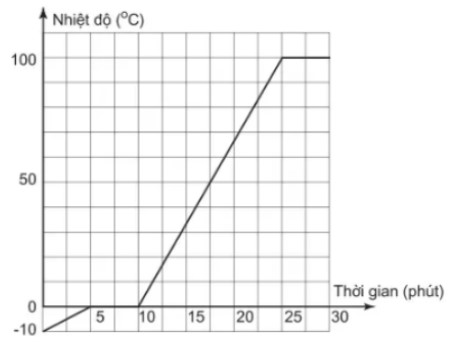
\includegraphics[width=0.45\linewidth]{figs/VN12-Y24-PH-SYL-001P-4}
\end{center}
\begin{enumerate}[label=\alph*)]
	\item Trong 5 phút đầu tiên, nước ở thể rắn.
	\item Từ phút thứ 5 đến phút thứ 10 nước đá nóng chảy.
	\item Từ phút thứ 10 đến phút thứ 25 nước không có sự bay hơi vì chưa đạt nhiệt độ sôi.
	\item Nước được đun ở điều kiện tiêu chuẩn.
\end{enumerate}
\loigiai{
	\begin{enumerate}[label=\alph*)]
		\item Đúng.
		\item Đúng.
		\item Sai. Nước bay hơi ở bất kì nhiệt độ nào.
		\item Đúng. Đồ thị thể hiện quá trình nước sôi ở $\SI{100}{\celsius}$.
	\end{enumerate}
}
\end{ex}

%=====================================================================================
\begin{ex}
	Bảng dưới đây ghi nhận nhiệt độ nóng chảy và nhiệt độ sôi của một số chất
	\begin{center}
		\begin{tabular}{|C{8em}|C{10em}|C{8em}|}
			\hline
			\thead{Chất}& \thead{Nhiệt độ nóng chảy} &\thead{Nhiệt độ sôi}\\
			\hline
			Chì & $\SI{327}{\celsius}$ & $\SI{1613}{\celsius}$\\
			\hline
			Nước & $\SI{0}{\celsius}$ & $\SI{100}{\celsius}$\\
			\hline
			Oxygen & $\SI{-219}{\celsius}$ & $\SI{-183}{\celsius}$\\
			\hline
			Rượu & $\SI{-117}{\celsius}$ & $\SI{78}{\celsius}$\\
			\hline
			Thuỷ ngân & $\SI{-39}{\celsius}$ & $\SI{357}{\celsius}$\\
			\hline
		\end{tabular}
	\end{center}
	\begin{enumerate}[label=\alph*)]
		\item Chì có nhiệt độ sôi cao nhất trong các chất được liệt kê.
		\item Nước có nhiệt độ sôi thấp nhất trong các chất được liệt kê.
		\item Ở nhiệt độ $\SI{30}{\celsius}$ thì chì ở thể  rắn.
		\item Ở nhiệt độ $\SI{30}{\celsius}$ thì oxide ở thể lỏng.
	\end{enumerate}
	\loigiai{
		\begin{enumerate}[label=\alph*)]
			\item Đúng.
			\item Sai.
			\item Đúng.
			\item Sai. 
		\end{enumerate}
	}
\end{ex}
%====================================================================================
\begin{ex}
	Hình bên là một cốc nước đá đặt ngoài không khí.
	\begin{center}
		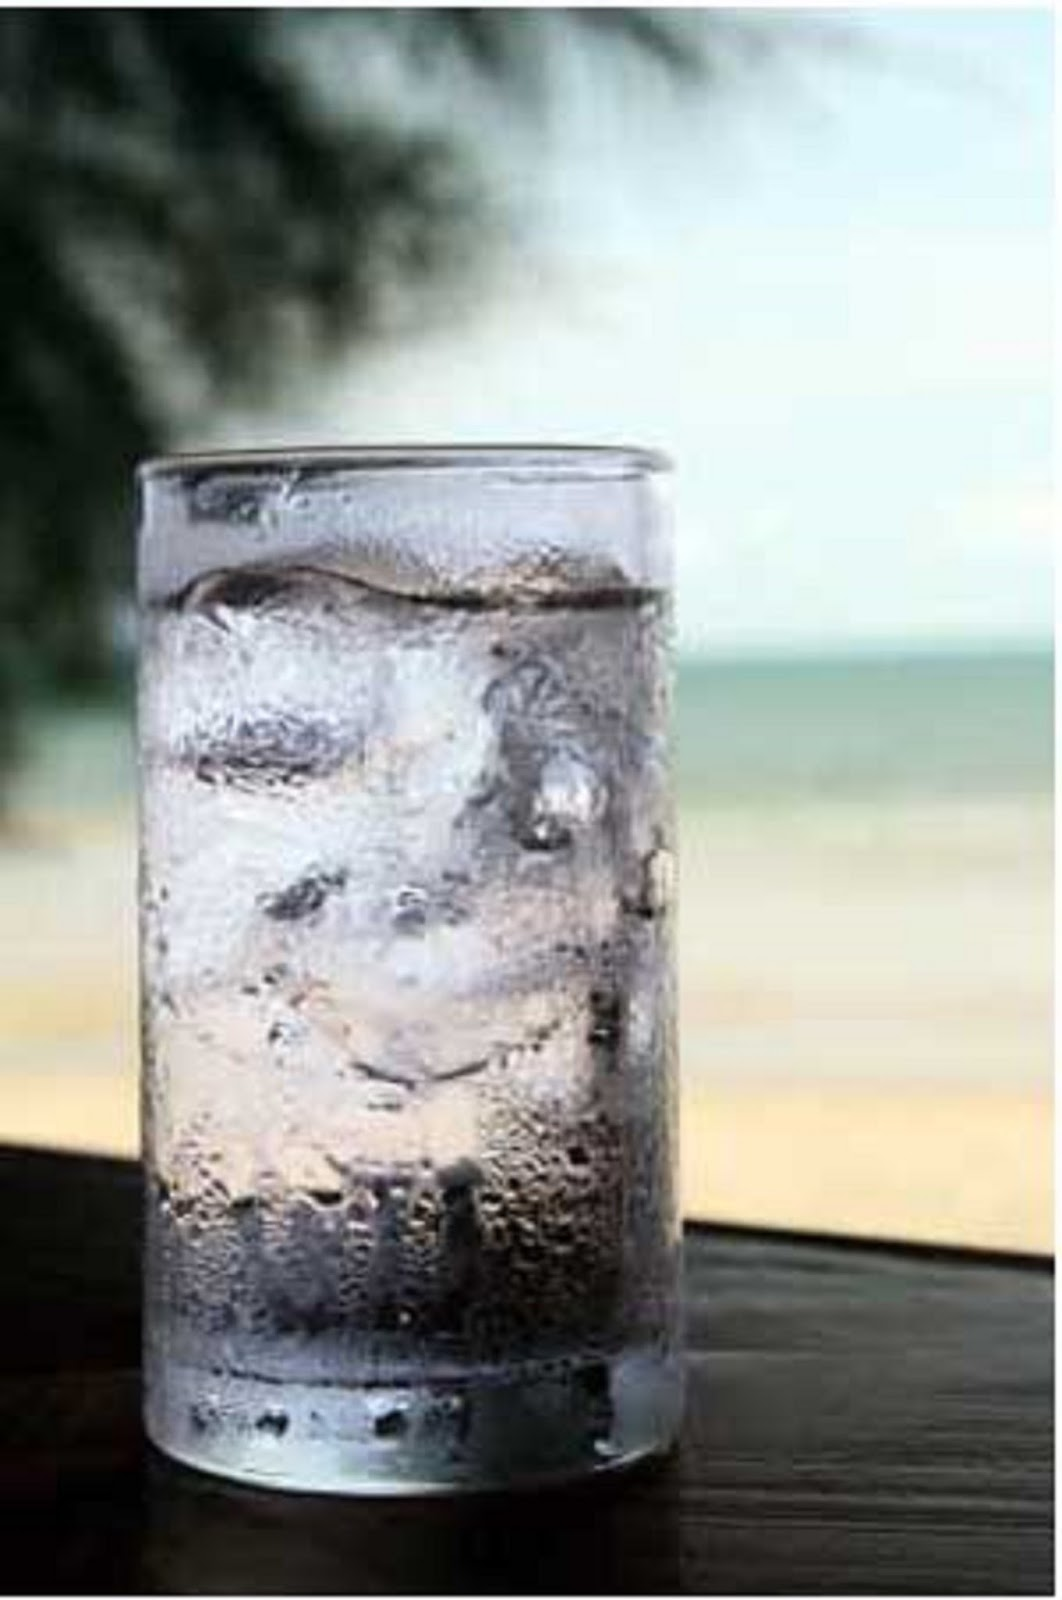
\includegraphics[width=0.2\linewidth]{figs/VN12-Y24-PH-SYL-001P-3}
	\end{center}

	\begin{enumerate}[label=\alph*)]
		\item 
		Nước ngưng đọng trên thành cốc là do nước bên trong cốc thấm ra ngoài.
		\item Nước đá truyền nhiệt ra bên ngoài làm đá tan dần.
		\item Khói trắng xuất hiện trên miệng cốc là do sự hoá hơi của nước trong cốc.
		\item Khi đá chưa tan hết thì nhiệt độ của nước trong cốc là $\SI{0}{\celsius}$.
	\end{enumerate}
	\loigiai{
		\begin{enumerate}[label=\alph*)]
			\item Sai. Nước đọng trên thành cốc là do hơi nước trong không khí gần cốc ngưng tụ.
			\item Sai. Nước đá nhận nhiệt từ môi trường nên tan dần.
			\item Sai. Khói trắng xuất hiện ở miệng cốc là kết quả sự ngưng tụ của hơi nước trong không khí.
			\item Đúng.
		\end{enumerate}
	}
	\end{ex}
\Closesolutionfile{ans}
\subsection{Bài tập tự luận}
\setcounter{ex}{0}
\begin{ex}
	Hãy sử dụng mô hình động học phân tử để giải thích vì sao chúng ta có thể đi trong không khí, bơi trong nước nhưng không thể đi xuyên qua tường?
	\loigiai{
		Lực liên kết giữa các phân tử chất rắn lớn hơn nhiều so với lực liên kết giữa các phân tử chất lỏng và chất khí. Do đó, ta khó bẽ gãy được liên kết của các phân tử chất rắn nên không thể đi xuyên qua tường.
		
	}
	\end{ex}
%=====================================================================================
\begin{ex}
Cùng một chất, khi ở thể lỏng thường có khối lượng riêng nhỏ hơn khi ở thể rắn và khối lượng riêng ở thế khí lại nhỏ hơn khi ở thể lỏng. Vì sao như vậy?
	\loigiai{Vì khoảng cách trung bình giữa các phân tử chất khí lớn hơn khoảng cách trung bình giữa các phân tử chất lỏng và lớn hơn khoảng cách trung bình giữa các phân tử chất rắn. Do đó, với cùng một chất thì thể khí thường có thể tích lớn hơn so với với thể lỏng và lớn hớn thể tích ở rắn. Vì vậy, ở thể lỏng thường có khối lượng riêng nhỏ hơn khi ở thể rắn và khối lượng riêng ở thế khí lại nhỏ hơn khi ở thể lỏng.}
\begin{note}
Không đúng cho tất cả trường hợp. Ví dụ, nước có thể tích ở thể rắn lớn hơn thể tích ở thể lỏng
\end{note}
	\end{ex}
%=====================================================================================
\begin{ex}
Cồn y tế chuyển từ thể lỏng sang thể khí rất nhanh ở điều kiện thông thường. Hãy giải thích tại sao khi xoa cồn vào da, ta cảm thấy lạnh ở vùng da đó?
	\loigiai{
		Khi cồn chuyển thể từ lỏng sang khí thì cần thu nhiệt lượng, do đó tay ta mất bớt nhiệt lượng truyền cho cồn và cảm thấy vùng da thoa cồn bị lạnh đi.
		
	}
	\end{ex}
%=====================================================================================
\begin{ex}
	Vì sao bình nước sôi muốn để nguội nhanh thì cần mở nắp để hơi nước thoát ra?
	\loigiai{
		Vì hơi nước có nhiệt độ cao, khi mở nắp thì hơi nước thoát ra nhiều và nhanh hơn làm cho nước còn lại trong bình dễ trao đổi nhiệt với không khí bên ngoài và giảm nhanh nhiệt độ.
	}
\end{ex}
%=====================================================================================
\begin{ex}
	Rau xanh sau khi mua về thường bị héo khi để ở ngoài trời nắng. Vì sao lại có hiện tượng trên? Làm thế nào để hạn chế điều này?
	\loigiai{
		Rau bị héo là do sự bay hơi của nước trong rau qua bề mặt lá. Để hạn chế rau nhanh héo có thể thực hiện các cách sau
		\begin{itemize}
			\item Tránh ánh nắng trực tiếp từ mặt trời, bảo quản ở nơi thoáng mát.
			\item Vẫy nước lên rau để tạo lớp nước bám trên bề mặt, lớp nước này sẽ hấp thụ nhiệt từ môi trường và bay hơi trước.
		\end{itemize}
		
	}
\end{ex}
%=====================================================================================
\begin{ex}
	Để khử trùng các dụng cụ y tế nhiều lần (kéo, kẹp gắp, dao mổ, \dots), ngày nay người ta thường sấy chúng trong lò sấy ở nhiệt độ cao. Tuy nhiên, trước đây người ta thường phải luộc chúng trong nước sôi. Giả sử cần phải thực hiện nhiệm vụ này nhưng có một số vi khuẩn chỉ bị tiêu diệt ở nhiệt độ $\SI{105}{\celsius}$, trong đó khi nhiệt độ sôi của nước ở điều kiện tiêu chuẩn là $\SI{100}{\celsius}$. Hãy đề xuất phương án đơn giản để diệt các vi khuẩn này và giải thích.
	\loigiai{
		Tăng áp suất đun nước (dùng nối áp suất) để tăng nhiệt độ sôi của nước.
	}
\end{ex}
%=====================================================================================
\begin{ex}
Một người thợ mộc sau khi đánh vecni vào một số chân giường, sau một thời gian, người thợ mộc phát hiện thấy những chân giường chưa được đánh vecni bị nứt (rạn chân chim), còn những chân giường đã được đánh vecni thì không bị như thế. Hãy giải thích tại sao?
	\loigiai{
		Trong gỗ có chứa một lượng nước nhất định, khi đánh vecni lên gỗ, lớp vecni ngăn cách sự tiếp xúc của gỗ với môi trường bên ngoài và làm hạn chế sự bay hơi của nước trong gỗ. Còn những chân giường không đánh vecni thì nước trong gỗ bị bay hơi và làm gỗ bị khô, nứt.
	}
\end{ex}
	
\newpage\section{NHIỆT ĐỘ - THANG NHIỆT ĐỘ}
\subsection{LÝ THUYẾT TRỌNG TÂM}
\subsubsection{Chiều truyền năng lượng nhiệt giữa hai vật chênh lệch nhiệt độ tiếp xúc nhau}
\begin{boxdn}
	Khi cho hai vật chênh lệch nhiệt độ tiếp xúc nhau, năng lượng nhiệt luôn truyền từ vật có nhiệt độ cao hơn sang vật có nhiệt độ thấp hơn. Quá trình truyền nhiệt kết thúc khi hai vật ở cùng nhiệt độ (trạng thái cân bằng nhiệt).
\end{boxdn}
\begin{center}
	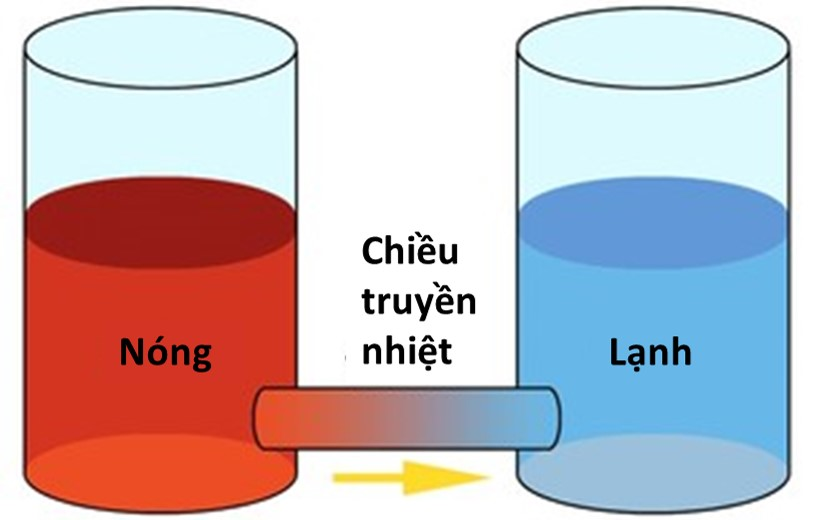
\includegraphics[width=0.3\linewidth]{figs/VN12-Y24-PH-SYL-002-1}
	\captionof{figure}{Minh hoạ chiều truyền nhiệt giữa hai vật có nhiệt độ khác nhau}
\end{center}
\subsubsection{Nhiệt độ}
\paragraph{Khái niệm về nhiệt độ}
\begin{boxdn}
	Nhiệt độ của một vật là đại lượng vật lí đặc trưng cho mức độ chuyển động nhiệt của phân tử vật chất cấu tạo nên vật. Khi các phân tử chuyển động nhiệt càng nhanh thì nhiệt độ của vật càng cao và ngược lại.
\end{boxdn}
\paragraph{Nhiệt kế}
\begin{boxdn}
	Nhiệt độ đo trên nhiệt kế được xác định thông qua giá trị của một đại lượng vật lí khác mà đại lượng này phụ thuộc theo nhiệt độ.
\end{boxdn}
\begin{boxvidu}
	\textbf{\textit{Ví dụ:}}
	\begin{itemize}
		\item Nhiệt kế thuỷ ngân xác định nhiệt độ dựa trên hiện tượng dãn nở vì nhiệt của thuỷ ngân.
		\item Nhiệt kế điện trở xác định nhiệt độ qua sự phụ thuộc của điện trở theo nhiệt độ.
	\end{itemize}
\end{boxvidu}
\begin{center}
	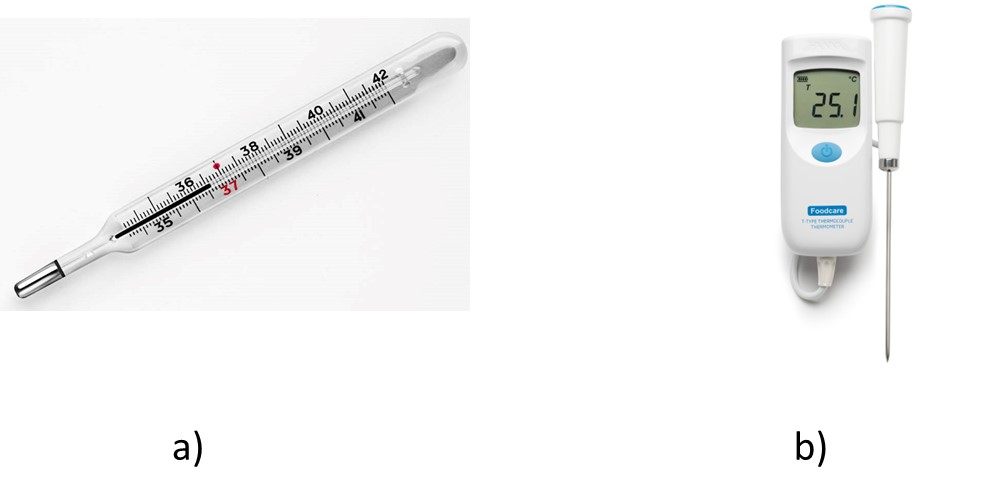
\includegraphics[width=0.5\linewidth]{figs/VN12-Y24-PH-SYL-002-2}
	\captionof{figure}{a) Nhiệt kế thuỷ ngân; b) Nhiệt kế điện trở}
\end{center}
\subsubsection{Thang nhiệt độ}
\paragraph{Thang nhiệt độ Celsius}
\begin{boxdn}
	Nhiệt độ trong thang đo này được kí hiệu là $t$. Đơn vị là độ Celsius (kí hiệu: $\si{\celsius}$).\\
	$\SI{1}{\celsius}=\dfrac{1}{100}$ của khoảng cách giữa nhiệt độ nóng chảy của nước tinh khiết đóng băng $\left(\SI{0}{\celsius}\right)$ và nhiệt độ sôi của nước tinh khiết ở áp suất $\SI{1}{atm}$ ($\SI{100}{\celsius}$).
\end{boxdn}

\paragraph{Thang nhiệt độ Kelvin}
\begin{boxdn}
	Nhiệt độ trong thang đo này được kí hiệu là $T$. Đơn vị là độ Kelvin (kí hiệu: $\si{\kelvin}$).\\
	$\SI{1}{\kelvin}=\dfrac{1}{273,15}$ của khoảng cách giữa nhiệt độ không tuyệt đối $\left(\SI{0}{\kelvin}\right)$ và nhiệt độ điểm mà nước tinh khiết tồn tại đồng thời ở thể rắn, lỏng và hơi ở áp suất $\SI{1}{atm}$ ($\SI{273.15}{\kelvin}$).\\
	Nhiệt độ không tuyệt đối ($\SI{0}{\kelvin}$) là nhiệt độ mà tại đó động năng chuyển động nhiệt của các phân tử cấu tạo nên vật chất bằng không và thế năng của chúng là tối thiểu.
\end{boxdn}
\begin{luuy}
	Một độ chia trên thang nhiệt độ Kelvin bằng một độ chia trên thang nhiệt độ Celsius.
\end{luuy}
\paragraph{Chuyển đổi nhiệt độ đo theo thang Celsius sang nhiệt độ đo theo thang Kelvin}
\begin{boxdl}
	\begin{equation}
		T=t+273,15\approx t+273
	\end{equation}
\end{boxdl}
với:
\begin{itemize}
	\item $t$: giá trị nhiệt độ của vật theo thang nhiệt độ Celsius;
	\item $T$: giá trị nhiệt độ của vật theo thang nhiệt độ Kelvin.
\end{itemize}
\subsection{VÍ DỤ MINH HOẠ}
\begin{dang}{Chuyển đổi được nhiệt độ đo theo thang Celsius sang nhiệt độ đo theo thang Kelvin và ngược lại}

\end{dang}
	\begin{vd}
Nhiệt độ của khối khí trong phòng đo được là $\SI{27}{\celsius}$. Xác định nhiệt độ của khối khí trong thang nhiệt độ Kelvin.
		\loigiai{
			Nhiệt độ khối khí trong thang nhiệt độ Kelvin:
			$$T=t+273=\SI{300}{\kelvin}.$$}
		
	
\end{vd}

\begin{vd}
	Một nhiệt kế dùng để đo nhiệt độ của các lò nung có phạm vi đo từ $\SI{263}{\kelvin}$ đến $\SI{1273}{\kelvin}$.
	\begin{enumerate}[label=\alph*)]
		\item Xác định phạm vi đo của nhiệt kế này trong thang nhiệt độ Celsius?
		\item Nếu sử dụng nhiệt kế này để đo nhiệt độ lò nung đang nấu chảy đồng có nhiệt độ nóng chảy là $\SI{1083}{\celsius}$ thì nhiệt kế có đo được không? Vì sao? Em có khuyến cáo gì về việc sử dụng nhiệt kế trong tình huống này?
	\end{enumerate}
	\loigiai{
		\begin{enumerate}[label=\alph*)]
			\item $t_\text{min}=T_\text{min}-273=\SI{-10}{\celsius};\quad t_\text{max}=T_\text{max}-273=\SI{1000}{\celsius}.$\\
			Phạm vi đo của nhiệt kế này trong thang nhiệt độ Celsius là $\SI{-10}{\celsius}$ đến $\SI{1000}{\celsius}$.
			\item Nếu sử dụng nhiệt kế này để đo nhiệt độ lò nung đang nấu chảy đồng có nhiệt độ nóng chảy $\SI{1083}{\celsius}$ thì nhiệt kế không đo được vì nhiệt độ cần đo nằm khoảng phạm vi đo của nhiệt kế.\\
			Trong trường hợp này, người đo cần dùng nhiệt kế có thang đo lớn hơn $\SI{1083}{\celsius}$ như nhiệt kế điện trở.
	\end{enumerate}}
\end{vd}

\begin{vd}
	Trong thang nhiệt độ Fahrenheit, chọn nhiệt độ tại điểm nước đá đang tan là $\SI{32}{\degree F}$, nhiệt độ tại điểm nước sôi ở điều kiện thường $\left(\SI{1}{atm}\right)$ là $\SI{212}{\degree F}$, trong khoảng nhiệt độ này chia thành 180 khoảng bằng nhau, mỗi khoảng ứng với $\SI{1}{\degree F}$. Thang đo này được nhà vật lí người Đức Daniel Gabriel Fahrenheit đề xuất vào năm 1724 và được sử dụng phổ biến ở các nước phương Tây. Nếu gọi $t$ là nhiệt độ của vật trong thang nhiệt độ Celsius và $T_\text{F}$ nhiệt độ của vật trong thang nhiệt độ Fahrenheit thì:
	$$T_\text{F}=a\cdot t+b.$$
	với $a$ và $b$ là các hệ số tỉ lệ.
	\begin{enumerate}[label=\alph*)]
		\item Em hãy xác định xác giá trị của $a$ và $b$.
		\item Trên tin tức thông báo nhiệt độ tại New York ngày 17/03/2024 là $\SI{49}{\degree F}$. Trong thang Celsius thì nhiệt độ này là bao nhiêu $\si{\celsius}$?
	\end{enumerate}
	\loigiai{
		\begin{enumerate}[label=\alph*)]
			\item Nhiệt độ tại điểm nước đá đang tan là $\SI{32}{\degree F}$ hay $\SI{0}{\celsius}$:
			\begin{equation}
				\label{eq: 1}\\
				b=\SI{32}{\degree F}
			\end{equation}
			Nhiệt độ tại điểm nước sôi ở điều kiện thường $\left(\SI{1}{atm}\right)$ là $\SI{212}{\degree F}$ hay $\SI{100}{\celsius}$:
			\begin{equation}
				\label{eq: 2}\\
				212=100a+b
			\end{equation}
			Từ (\ref{eq: 1}) và (\ref{eq: 2}), suy ra:
			\begin{equation*}
				\begin{cases}
					b=\SI{32}{\degree F}\\
					a=\SI{1.8}{\degree F/\celsius}
				\end{cases}
			\end{equation*}
			Như vậy, $T_\text{F}=1,8\cdot t+32.$
			\item Nhiệt độ tại New York ngày 17/03/2024 theo thang Celsius:
			$$t=\dfrac{T_\text{F}-32}{1,8}\approx\SI{9.44}{\celsius}.$$
	\end{enumerate}}
\end{vd}
\begin{luuy}
	$$\dfrac{t\left(\si{\degree F}\right)-32}{212-32}=\dfrac{t\left(\si{\celsius}\right)-0}{100-0}=\dfrac{T\left(\si{\kelvin}\right)-273}{373-273}.$$
\end{luuy}
\subsection{BÀI TẬP TRẮC NGHIỆM}
\inputansbox{10}{ans/G12Y24B2TN}
\Opensolutionfile{ans}[ans/G12Y24B2TN]
\begin{ex}
	Cho hai vật có nhiệt độ khác nhau tiếp xúc với nhau. Nhiệt được truyền từ
	\choice
	{vật có khối lượng lớn hơn sang vật có khối lượng nhỏ hơn}
	{\True vật có nhiệt độ cao hơn sang vật có nhiệt độ thấp hơn}
	{vật ở trên cao sang vật ở dưới thấp}
	{vật có khối lượng riêng lớn sang vật có khối lượng riêng nhỏ}
	\loigiai{

}
	\end{ex}
%====================================================================================
\begin{ex}
Người ta cho hai vật dẫn nhiệt A và B tiếp xúc với nhau, sau một thời gian khi có trạng thái cân bằng nhiệt thì hai vật này có
	\choice
	{\True cùng nhiệt độ}
	{cùng nội năng}
	{cùng năng lượng}
	{cùng nhiệt lượng}
	\loigiai{
	
}
\end{ex}

%====================================================================================
\begin{ex}
Đơn vị đo nhiệt độ trong thang nhiệt Celsius là
	\choice
	{$\si{\kelvin}$}
	{$\si{\degree F}$}
	{$\si{\newton}$}
	{\True $\si{\celsius}$}
	\loigiai{
		
	}
\end{ex}
%====================================================================================
\begin{ex}
	Nhiệt kế chất lỏng được chế tạo dựa trên nguyên tắc nào?
	\choice
	{\True Sự nở vì nhiệt của chất lỏng}
	{Sự phụ thuộc của tốc độ dòng chảy theo nhiệt độ}
	{Sự thay đổi điện trở của khối chất lỏng theo nhiệt độ}
	{Sự phụ thuộc của áp suất chất lỏng theo nhiệt độ}
	\loigiai{
		
	}
\end{ex}
%====================================================================================
\begin{ex}
Trong các nhiệt kế sau đây, em hãy chọn nhiệt kế phù hợp để đo nhiệt độ của nước đang được đun sôi?
	\choice
	{Nhiệt kế y tế có thang chia độ từ $\SI{35}{\celsius}$ đến $\SI{42}{\celsius}$}
	{ Nhiệt kế rượu có thang chia độ từ $\SI{-30}{\celsius}$ đến $\SI{60}{\celsius}$}
	{\True Nhiệt kế thuỷ ngân có thang chia độ từ $\SI{-10}{\celsius}$ đến $\SI{110}{\celsius}$}
	{Nhiệt kế hồng ngoại có thang chia độ từ $\SI{30}{\celsius}$ đến $\SI{45}{\celsius}$}
	\loigiai{
		
	}
\end{ex}
%====================================================================================
\begin{ex}
	Cách xác định nhiệt độ trong thang nhiệt độ Celsius là
	\choice
	{Lấy nhiệt độ của nước khi đóng băng là $\left(\SI{10}{\celsius}\right)$ và nhiệt độ sôi của nước $\left(\SI{100}{\celsius}\right)$ làm chuẩn}
	{Lấy nhiệt độ của nước khi đóng băng là $\left(\SI{100}{\celsius}\right)$ và nhiệt độ sôi của nước $\left(\SI{0}{\celsius}\right)$ làm chuẩn}
	{\True Lấy nhiệt độ của nước khi đóng băng là $\left(\SI{0}{\celsius}\right)$ và nhiệt độ sôi của nước $\left(\SI{100}{\celsius}\right)$ làm chuẩn}
	{Lấy nhiệt độ của nước khi đóng băng là $\left(\SI{100}{\celsius}\right)$ và nhiệt độ sôi của nước $\left(\SI{10}{\celsius}\right)$ làm chuẩn}
	\loigiai{
		
	}
\end{ex}
%====================================================================================
\begin{ex}
	Điểm đóng băng và sôi của nước theo thang Kelvin là
	\choice
	{$\SI{0}{\kelvin}$ và $\SI{100}{\kelvin}$}
	{\True $\SI{273}{\kelvin}$ và $\SI{373}{\kelvin}$}
	{$\SI{37}{\kelvin}$ và $\SI{73}{\kelvin}$}
	{$\SI{32}{\kelvin}$ và $\SI{212}{\kelvin}$}
	\loigiai{
		
	}
\end{ex}

%====================================================================================
\begin{ex}
	Độ không tuyệt đối là nhiệt độ ứng với
	\choice
	{\True $\SI{0}{\kelvin}$}
	{$\SI{0}{\celsius}$}
	{$\SI{273}{\kelvin}$}
	{$\SI{273}{\celsius}$}
	\loigiai{
		
	}
\end{ex}
%====================================================================================
\begin{ex}
	Chọn phát biểu \textbf{đúng}.\\
	Nhiệt độ không tuyệt đối là nhiệt độ mà tại đó
	\choice
	{\True chuyển động nhiệt của phân tử hầu như dừng lại}
	{nước bắt đầu đông thành đá}
	{tất cả chất khí hoá lỏng}
	{tất cả chất khí hoá rắn}
	\loigiai{
		
	}
\end{ex}
%====================================================================================
\begin{ex}
Không thể dùng nhiệt kế rượu để đo nhiệt độ của nước đang sôi vì
	\choice
	{rượu sôi ở nhiệt độ cao hơn $\SI{100}{\celsius}$}
	{\True rượu sôi ở nhiệt độ thấp hơn $\SI{100}{\celsius}$}
	{rượu đông đặc ở nhiệt độ $\SI{100}{\celsius}$}
	{rượu đông đặc ở nhiệt độ thấp hơn $\SI{0}{\celsius}$}
	\loigiai{
		
	}
\end{ex}
%====================================================================================
\begin{ex}
Biểu thức nào sau đây là đúng khi biến đổi nhiệt độ từ thang Celsius sang thang Kelvin?
	\choice
	{$T\left(\si{\kelvin}\right)=t\left(\si{\celsius}\right)-273$}
	{\True $T\left(\si{\kelvin}\right)=t\left(\si{\celsius}\right)+273$}
	{$T\left(\si{\kelvin}\right)=\dfrac{t\left(\si{\celsius}\right)+273}{2}$}
	{$T\left(\si{\kelvin}\right)=2t\left(\si{\celsius}\right)+273$}
	\loigiai{
		
	}
\end{ex}
%====================================================================================
\begin{ex}
Cho các bước như sau:
\begin{enumerate}[label=(\arabic*)]
	\item Thực hiện phép đo nhiệt độ.
	\item Ước lượng nhiệt độ của vật.
	\item Hiệu chỉnh nhiệt kế.
	\item Lựa chọn nhiệt kế phù hợp.
	\item Đọc và ghi kết quả đo.
\end{enumerate}
Các bước đúng khi thực hiện đo nhiệt độ của một vật là
	\choice
	{\True (2), (4), (3), (1), (5)}
	{(1), (4), (2), (3), (5)}
	{(1), (2), (3), (4), (5)}
	{(3), (2), (4), (1), (5)}
	\loigiai{
		
	}
\end{ex}
%====================================================================================
\begin{ex}
Nhiệt độ trung bình của nước ở thang nhiệt độ Celsius là $\SI{27}{\celsius}$ ứng với thang nhiệt độ Kelvin thì nhiệt độ của nước là
	\choice
	{$\SI{273}{\kelvin}$}
	{\True $\SI{300}{\kelvin}$}
	{$\SI{246}{\kelvin}$}
	{$\SI{327}{\kelvin}$}
	\loigiai{
			$$T=t+273=\SI{300}{\kelvin}.$$
	}
\end{ex}
%====================================================================================
\begin{ex}
Nhiệt độ mùa đông tại thành phố New York (Mỹ) là $\SI{283}{\kelvin}$, ứng với nhiệt giai Celsius thì nhiệt độ ở đó là
	\choice
	{\True $\SI{10}{\celsius}$}
	{$\SI{-10}{\celsius}$}
	{$\SI{5}{\celsius}$}
	{$\SI{-5}{\celsius}$}
	\loigiai{
		$$t=T-273=\SI{10}{\celsius}.$$
	}
\end{ex}


%====================================================================================
\begin{ex}
	Nhiệt độ vào một ngày mùa hè ở thành phố Hồ Chí Minh là $\SI{35}{\celsius}$. Nhiệt độ đó tương ứng với bao nhiêu độ $\si{\degree F}$?
	\choice
	{$\SI{59}{\degree F}$}
	{$\SI{67}{\degree F}$}
	{\True $\SI{95}{\degree F}$}
	{$\SI{76}{\degree F}$}
	\loigiai{
		$$t\left(\si{\degree F}\right)=32+1,8t\left(\si{\celsius}\right)=\SI{95}{\degree F}.$$
	}
\end{ex}
%====================================================================================
\begin{ex}
	Giá trị nhiệt độ đo được theo thang nhiệt độ Kelvin là $\SI{293}{\kelvin}$. Tính theo thang nhiệt độ Fahrenheit, nhiệt độ đó có giá trị là
	\choice
	{$\SI{20}{\degree F}$}
	{$\SI{100}{\degree F}$}
	{\True $\SI{68}{\degree F}$}
	{$\SI{261}{\degree F}$}
	\loigiai{
		$$t\left(\si{\celsius}\right)=T-273=\SI{20}{\celsius}.$$
	$$t\left(\si{\degree F}\right)=32+1,8t\left(\si{\celsius}\right)=\SI{68}{\degree F}.$$}
\end{ex}
%====================================================================================
\begin{ex}
	$\SI{104}{\degree F}$ ứng với bao nhiêu độ Kelvin?
	\choice
	{\True $\SI{313}{\kelvin}$}
	{$\SI{298}{\kelvin}$}
	{$\SI{328}{\kelvin}$}
	{$\SI{293}{\kelvin}$}
	\loigiai{
		$$\dfrac{t\left(\si{\degree F}\right)-32}{212-32}=\dfrac{T\left(\si{\kelvin}\right)-273}{373-273}$$
		Thay $t\left(\si{\degree F}\right)=\SI{104}{\degree F}$, thu được $T=\SI{313}{\kelvin}.$}
	\end{ex}
%====================================================================================
\begin{ex}
	Một thang đo $X$ lấy điểm đóng băng là $-10X$, lấy điểm sôi là $90X$. Nhiệt độ của một vật đọc được trên theo nhiệt giai Celsius là $\SI{40}{\celsius}$ thì trong nhiệt giai $X$ có nhiệt độ bằng
	\choice
	{$20X$}
	{\True $30X$}
	{$40X$}
	{$50X$}
	\loigiai{
		Độ chênh lệch nhiệt độ tại điểm băng và điểm sôi trong thang X cũng là 100. Như vậy $\SI{1}{\celsius}$ tương ứng với $\SI{1}{X}$ và
		$$t\left(\si{\celsius}\right)=t\left(\si{X}\right)+10.$$
	}
\end{ex}
%====================================================================================
\begin{ex}
	Giả sử có một thang nhiệt độ kí hiệu Z. Nhiệt độ sôi của nước theo thang này là $60Z$, điểm ba cả nước là $-15Z$. Nhiệt độ của vật theo thang Fahrenheit là bao nhiêu nếu nhiệt độ trong thang Z là $-96Z$?Giả sử có một thang nhiệt độ kí hiệu Z. Nhiệt độ sôi của nước theo thang này là $60Z$, điểm ba cả nước là $-15Z$. Nhiệt độ của vật theo thang Fahrenheit là bao nhiêu nếu nhiệt độ trong thang Z là $-96Z$?
	\choice
	{$\SI{-62.4}{\degree F}$}
	{$\SI{162.4}{\degree F}$}
	{\True $\SI{-162.4}{\degree F}$}
	{$\SI{62.4}{\degree F}$}
	\loigiai{
	$$\dfrac{t\left(\si{\degree F}\right)-32}{212-32}=\dfrac{Z-\left(-15\right)}{60-\left(-15\right)}$$
	Thay $Z=-96$ ta thu được $t\left(\si{\degree F}\right)=\SI{-162.4}{\degree F}.$
	}
\end{ex}
%====================================================================================
\begin{ex}
Hình dưới thể hiện nhiệt kế đo nhiệt độ của một vật. Sai số dụng cụ được lấy bằng một nửa độ chia nhỏ nhất. Kết quả đo nhiệt độ của vật này là
\begin{center}
	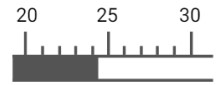
\includegraphics[width=0.25\linewidth]{figs/VN12-Y24-PH-SYL-002P-3}
\end{center}
	\choice
	{\True $t=\xsi{24.0\pm0.5}{\celsius}$}
	{$t=\xsi{25.0\pm0.5}{\celsius}$}
	{$t=\xsi{24.0\pm1.0}{\celsius}$}
	{$t=\xsi{25.0\pm1.0}{\celsius}$}
	\loigiai{
		
	}
\end{ex}

%====================================================================================
\begin{ex}
Chiều dài của phần thuỷ ngân trong nhiệt kế là $\SI{2}{\centi\meter}$ ở $\SI{0}{\celsius}$ và $\SI{22}{\centi\meter}$ ở $\SI{100}{\celsius}$. Nhiệt độ là bao nhiêu nếu chiều dài của thuỷ ngân là $\SI{8}{\centi\meter}$?
	\choice
	{$\SI{40}{\celsius}$.$\SI{40}{\celsius}$}
	{$\SI{50}{\celsius}$}
	{$\SI{20}{\celsius}$}
	{\True $\SI{30}{\celsius}$}
	\loigiai{
		$$\dfrac{\ell-\ell_0}{t-t_0}=\dfrac{\ell'-\ell_0}{t'-t_0}$$
		$$\Leftrightarrow\dfrac{\SI{22}{\centi\meter}-\SI{2}{\centi\meter}}{\SI{100}{\celsius}-\SI{0}{\celsius}}=\dfrac{\SI{8}{\centi\meter}-\SI{2}{\centi\meter}}{t'-\SI{0}{\celsius}}\Rightarrow t'=\SI{30}{\celsius}.$$
	}
\end{ex}
%====================================================================================
\begin{ex}
Chiều dài của phần thuỷ ngân trong nhiệt kế là $\SI{2}{\centi\meter}$ ở $\SI{0}{\celsius}$ và $\SI{22}{\centi\meter}$ ở $\SI{100}{\celsius}$. Chiều dài của phần thuỷ ngân sẽ là bao nhiêu nếu nhiệt độ là $\SI{50}{\celsius}$?
	\choice
	{$\SI{10}{\centi\meter}$}
	{\True $\SI{12}{\centi\meter}$}
	{$\SI{14}{\centi\meter}$}
	{$\SI{16}{\centi\meter}$}
	\loigiai{
	$$\dfrac{\ell-\ell_0}{t-t_0}=\dfrac{\ell'-\ell_0}{t'-t_0}$$
	$$\Leftrightarrow\dfrac{\SI{22}{\centi\meter}-\SI{2}{\centi\meter}}{\SI{100}{\celsius}-\SI{0}{\celsius}}=\dfrac{\ell'-\SI{2}{\centi\meter}}{\SI{50}{\celsius}-\SI{0}{\celsius}}\Rightarrow \ell'=\SI{12}{\centi\meter}.$$
	}
\end{ex}
%====================================================================================
\begin{ex}
Sự phụ thuộc vào nhiệt độ của bước sóng điện từ theo hệ thức Wien: $T\cdot\lambda_\text{max}=\SI{2900}{\left(\micro\meter\cdot\kelvin\right)}$ được dùng vào việc chế tạo các nhiệt kế thường dùng hằng ngày như
nhiệt kế hồng ngoại, cũng như các nhiệt kế trong thiên văn để đo nhiệt độ bề mặt của
các thiên thể. Xét một nhiệt kế hồng ngoại khi đo nhiệt độ cơ thể người như hình vẽ.
Bước sóng hồng ngoại do cơ thể người phát ra bằng xấp xỉ bằng
\begin{center}
	
\includegraphics[width=0.3\linewidth]{figs/VN12-Y24-PH-SYL-002P-1}
\end{center}
	\choice
	{\True $\SI{9.4}{\micro\meter}$}
	{$\SI{79}{\micro\meter}$}
	{$\SI{29}{\micro\meter}$}
	{$\SI{10.6}{\micro\meter}$}
	\loigiai{
	$$\lambda_\text{max}=\dfrac{\SI{2900}{\micro\meter\cdot\kelvin}}{T}=\dfrac{\SI{2900}{\micro\meter\cdot\kelvin}}{36,5+\SI{273}{\kelvin}}\approx\SI{9.4}{\micro\meter}.$$
	}
\end{ex}
\Closesolutionfile{ans}
\subsection{TRẮC NGHIỆM ĐÚNG/SAI}
\setcounter{ex}{0}

\begin{ex}
		Bảng sau đây ghi sự thay đổi nhiệt độ của không khí theo thời gian dựa trên số liệu của một trạm khí tượng ở Hà Nội ghi được vào một ngày mùa đông.
	\begin{center}
		\begin{tabular}{|C{8em}|C{1.5em}|C{1.5em}|C{1.5em}|C{1.5em}|C{1.5em}|C{1.5em}|C{1.5em}|C{1.5em}|}
			\hline
			\thead{Thời gian (giờ)}& 1 & 4 & 7 & 10 & 13 & 16 & 19 & 22\\
			\hline
			\thead{Nhiệt độ $\left(\si{\celsius}\right)$} & 13 & 13 &13 & 18& 18 & 20 & 17 & 12\\
			\hline
		\end{tabular}
	\end{center}
	\begin{enumerate}[label=\alph*)]
		\item Nhiệt độ lúc 4 giờ là $\SI{286}{\kelvin}$.
		\item Nhiệt độ thấp nhất trong ngày là vào lúc 1 giờ.
		\item Nhiệt độ cao nhất trong ngày là vào lúc 16 giờ.
		\item Độ chênh lệch nhiệt độ trong ngày là $\SI{6}{\celsius}$.
	\end{enumerate}
	\loigiai{
	\begin{enumerate}[label=\alph*)]
		\item Đúng.
		\item Sai. Nhiệt độ thấp nhất là $\SI{12}{\celsius}$ vào lúc $\SI{22}{\hour}$.
		\item Đúng.
		\item Sai. Độ chênh lệch nhiệt độ trong ngày là $\SI{8}{\celsius}$.
	\end{enumerate}
	
}
	\end{ex}

% =================================================================================
\begin{ex}
	Bảng dưới đây ghi tên các loại nhiệt kế và thang đo của chúng
	\begin{center}
		\begin{tabular}{|C{5cm}|C{6cm}|}
			\hline
			\thead{Loại nhiệt kế} & \thead{Thang nhiệt độ}\\
			\hline
			Thuỷ ngân & Từ $\SI{-10}{\celsius}$ đến $\SI{110}{\celsius}$\\
			\hline
			Rượu & Từ $\SI{-30}{\celsius}$ đến $\SI{60}{\celsius}$\\
			\hline
			Kim loại & Từ $\SI{0}{\celsius}$ đến $\SI{400}{\celsius}$\\
			\hline
			Điện tử & Từ $\SI{34}{\celsius}$ đến $\SI{42}{\celsius}$\\
			\hline
		\end{tabular}
	\end{center}
	\begin{enumerate}[label=\alph*)]
		\item Dùng nhiệt kế kim loại để đo nhiệt độ nước sôi.
		\item Dùng nhiệt kế điện tử để đo nhiệt độ cơ thể người.
		\item Dùng nhiệt kế thuỷ ngân để đo nhiệt độ không khí trong phòng.
		\item Dùng nhiệt kế rượu để đo nhiệt độ bề mặt bàn là.
	\end{enumerate}
	\loigiai{
	\begin{enumerate}[label=\alph*)]
		\item Đúng.
		\item Đúng.
		\item Đúng.
		\item Sai.
	\end{enumerate}
}
	\end{ex}
% ================================================================================
	\begin{ex}
		Hình bên là một nhiệt kế rượu.
		\begin{center}
			
\includegraphics[width=0.25\linewidth]{figs/VN12-Y24-PH-SYL-002P-2}
		\end{center}
		\begin{enumerate}[label=\alph*)]
			\item Giới hạn đo của nhiệt kế là $\SI{120}{\celsius}$.
			\item Độ chia nhỏ nhất của nhiệt kế là $\SI{5}{\celsius}$.
			\item Nhiệt độ hiện tại trên nhiệt kế là $\SI{19}{\celsius}$.
			\item Có thể dùng nhiệt kế để xác định nhiệt độ của nước sôi.
		\end{enumerate}
		\loigiai{
		\begin{enumerate}[label=\alph*)]
			\item Sai. Giới hạn đo của nhiệt kế là $\SI{50}{\celsius}$.
			\item Đúng.
			\item Sai. ĐCNN của nhiệt kế là $\SI{5}{\celsius}$ nên không thể đọc được giá trị $\SI{19}{\celsius}$, nhiệt độ hiện tại có thể đọc từ nhiệt kế là $\SI{20}{\celsius}$.
			\item Sai. Giới hạn đo của nhiệt kế nhỏ hơn nhiệt độ nước sôi.
		\end{enumerate}
	}

		\end{ex}
\subsection{BÀI TẬP TỰ LUẬN}
\setcounter{ex}{0}
\begin{ex}
	Theo dự báo thời tiết ngày 17/04/2024 thì nhiệt độ trung bình ngày - đêm trong
	ngày hôm đó tại Thành phố Hồ Chí Minh là  $\SI{35}{\celsius}-\SI{25}{\celsius}$. Sự chênh lệch nhiệt độ này trong thang đo Kelvin là bao nhiêu $\si{\kelvin}$?
	\loigiai{
		$$\Delta T=\SI{10}{\kelvin}.$$	
}
	\end{ex}

% ===================================================================================
\begin{ex}
	Thế giới từng ghi nhận sự thay đổi nhiệt độ rất lớn diễn ra ở Spearfish, South Dakota vào ngày 22/01/1943. Lúc 7h30 sáng, nhiệt độ ngoài trời là $\SI{-20}{\celsius}$. Hai phút sau, nhiệt độ ngoài trời tăng lên đến $\SI{7.2}{\celsius}$. Xác định độ tăng nhiệt độ trung bình trong 2 phút đó theo đơn vị Kelvin/giây.
	\loigiai{
		$$\dfrac{\Delta T}{t}=\dfrac{\SI{27.2}{\kelvin}}{\SI{120}{\second}}\approx\SI{0.23}{\kelvin/\second}.$$
	}
	\end{ex}
% ===================================================================================
\begin{ex}
Ở $\SI{20}{\celsius}$ một thanh nhôm dài $\SI{12}{\meter}$. Tính nhiệt độ cần thiết để chiều dài thanh nhôm là $\SI{12.01}{\meter}$. Biết rằng khi nhiệt độ tăng thêm $\SI{1}{\celsius}$ thì thanh nhôm dài thêm $\SI{2.3E-5}{}$ chiều dài ban đầu.
\loigiai{
	$$\Delta\ell=\alpha\ell_0\Delta t$$
	với $\alpha=\SI{2.3E-5}{\kelvin^{-1}}$.
	$$\Rightarrow \Delta t=\dfrac{\Delta \ell}{\alpha\ell_0}=\SI{36.23}{\celsius}.$$
	Vậy nhiệt độ cần thiết để thanh nhôm dài $\SI{12.01}{\meter}$ là $\SI{56.23}{\celsius}$.
}
\end{ex}


% ===================================================================================
\begin{ex}
Một nhiệt kế thể tích không đổi hiển thị nhiệt độ $\SI{0}{\celsius}$ và $\SI{100}{\celsius}$ với các áp suất $\SI{60}{\centi\meter Hg}$ và $\SI{120}{\centi\meter Hg}$. Biết nhiệt độ đọc được là hàm bậc nhất của áp suất. Khi áp suất thuỷ ngân là $\SI{90}{\centi\meter Hg}$ thì nhiệt độ đọc được bằng bao nhiêu?
\loigiai{
	Ta có:
	$$t=a\cdot p+b\Rightarrow \dfrac{t-t_1}{t_2-t_1}=\dfrac{p-p_1}{p_2-p_1}.$$
	Thay $p=\SI{90}{\centi\meter Hg}$; $t_1=\SI{0}{\celsius}$; $t_2=\SI{100}{\celsius}$; $p_1=\SI{60}{\centi\meter Hg}$; $p_2=\SI{120}{\centi\meter Hg}$, ta thu được: $t=\SI{50}{\celsius}.$
}

\end{ex}



	
\newpage\section{NỘI NĂNG - ĐỊNH LUẬT I NHIỆT ĐỘNG LỰC HỌC}
\subsection{LÝ THUYẾT TRỌNG TÂM}
\subsubsection{Nội năng}
\paragraph{Khái niệm nội năng}
\begin{boxdn}
	Nội năng của một vật là tổng động năng và thế năng tương tác của các phân tử cấu tạo nên vật. Nội năng của vật phụ thuộc vào nhiệt độ $T$ và thể tích $V$ của vật:
	$$U=f\left(T, V\right).$$
\end{boxdn}
Đơn vị của nội năng trong hệ SI là joule $\left(\si{\joule}\right)$.
\paragraph{Mối liên hệ giữa nội năng và năng lượng của các phân tử cấu tạo nên vật}
Khi năng lượng của các phân tử cấu tạo nên vật tăng thì nội năng của vật tăng và ngược lại.
\subsubsection{Các cách làm thay đổi nội năng}
\paragraph{Thực hiện công}
\begin{boxdn}
	Quá trình thực hiện công làm cho nội năng của hệ thay đổi, hệ nhận công thì nội năng của hệ tăng, hệ thực hiện công cho vật khác thì nội năng giảm.
\end{boxdn}
\begin{boxvidu}
	\textbf{\textit{Ví dụ 1:}} Dùng tay ấn mạnh và nhanh piston của một cylanh chứa khí, thể tích khí trong cylanh giảm xuống (thế năng tương tác giữa các phân tử khí tăng), đồng thời khí nóng lên (động năng chuyển động nhiệt của các phân tử khí tăng). Do đó, nội năng của khí tăng.
\end{boxvidu}
\begin{boxvidu}
	\textbf{\textit{Ví dụ 2:}} Chà xát hai thanh gỗ với nhau, bề mặt tiếp xúc của hai thanh gỗ nóng dần lên. Nội năng của thanh gỗ tăng.
\end{boxvidu}
\begin{center}
	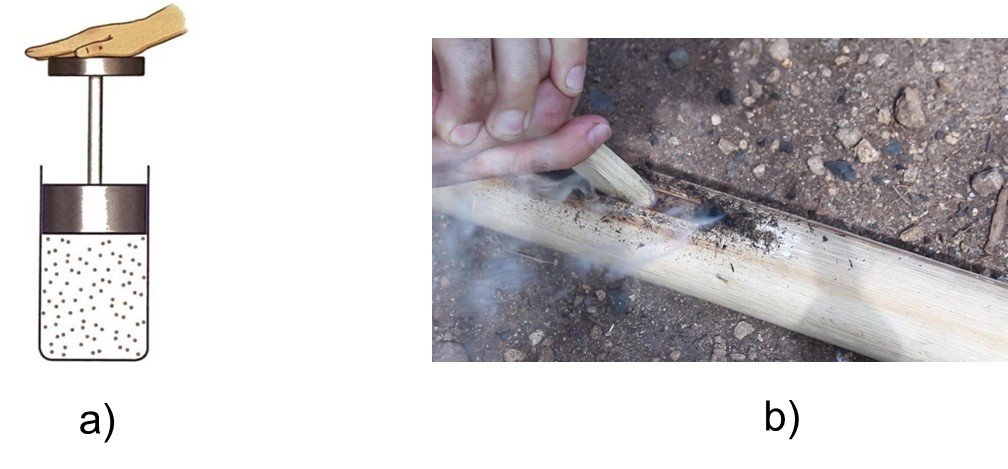
\includegraphics[width=0.45\linewidth	]{figs/VN12-Y24-PH-SYL-003-1}
	\captionof{figure}{a) Nén khối khí trong cylanh; b) Chà xát hai thanh gỗ với nhau}
\end{center}
\paragraph{Truyền nhiệt}
\begin{boxdn}
	Quá trình làm thay đổi nội năng của vật bằng cách cho nó tiếp xúc với vật khác khi có sự chênh lệch nhiệt độ giữa chúng gọi là sự truyền nhiệt.
\end{boxdn}
\begin{boxvidu}
	\textbf{\textit{Ví dụ:}} Miếng sắt sau khi tôi luyện được thả vào chậu nước để làm nguội đi. Khi đó, nước nhận nhiệt lượng từ miếng sắt nên nội năng tăng (nhiệt độ tăng) và miếng sắt truyền nhiệt lượng cho nước nên nội năng giảm (nhiệt độ giảm).
\end{boxvidu}
\begin{center}
	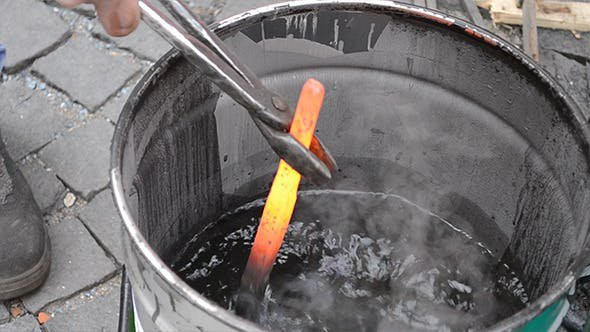
\includegraphics[width=0.3\linewidth]{figs/VN12-Y24-PH-SYL-003-2}
	\captionof{figure}{Miếng sắt nung được thả vào chậu nước}
\end{center}
\subsubsection{Định luật I nhiệt động lực học}
\begin{boxdl}
	Độ biến thiên nội năng của hệ bằng tổng công và nhiệt lượng mà hệ nhận được:
	\begin{equation}
		\Delta U= A+Q
	\end{equation}
\end{boxdl}
Trong đó:
\begin{itemize}
	\item $\Delta U$: độ biến thiên nội năng của hệ, đơn vị trong hệ SI là joule $\left(\si{\joule}\right)$;
	\item $A$: công mà hệ nhận/thực hiện, đơn vị trong hệ SI là joule $\left(\si{\joule}\right)$;
	\begin{itemize}[label=+]
		\item $A>0$: hệ nhận công;
		\item $A<0$: hệ thực hiện công.
	\end{itemize}
	\item $Q$: nhiệt lượng hệ trao đổi với bên ngoài, đơn vị trong hệ SI là joule $\left(\si{\joule}\right)$;
	\begin{itemize}[label=+]
		\item $Q>0$: hệ nhận nhiệt lượng;
		\item $Q<0$: hệ truyền nhiệt lượng.
	\end{itemize}
\end{itemize}
\begin{center}
	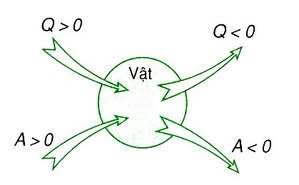
\includegraphics[width=0.35\linewidth]{figs/VN12-Y24-PH-SYL-003-3}
	\captionof{figure}{Quy ước về dấu của $Q$ và $A$}
\end{center}
\subsection{VÍ DỤ MINH HOẠ}
\begin{dang}{Trình bày được các cách làm thay đổi nội năng}
	
\end{dang}
		\begin{vd}
		Dựa vào mô hình động học phân tử, hãy giải thích hiện tượng quả bóng bàn bị móp (nhưng chưa bị thủng) khi thả vào cốc nước nóng sẽ phồng trở lại.
			\begin{center}
				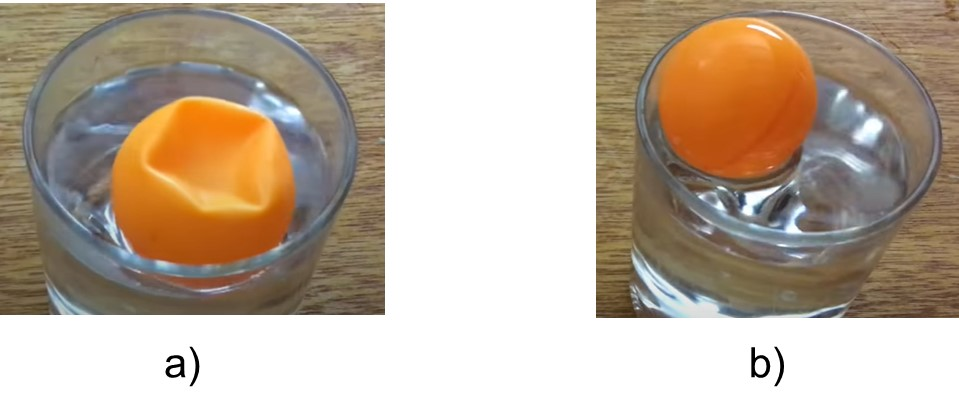
\includegraphics[width=0.45\linewidth]{{figs/VN12-Y24-PH-SYL-003-4}}
				\captionof{figure}{a) Quả bóng bàn ban đầu bị móp; b) Quả bóng sau khi được ngâm vào cốc nước nóng}
			\end{center}
			\loigiai{
				Khi thả quả bóng bi móp vào nước nóng, nhiệt độ khí trong quả bóng tăng làm các phân tử khí chuyển động nhiệt nhanh hơn nên va chạm với thành bóng nhiều hơn và mạnh hơn. Khi đó, áp suất khí trong quả bóng tăng lên và tạo ra lực đẩy đủ lớn làm vỏ cao su của quả bóng phồng trở lại}
	\end{vd}
		
		\begin{vd}
			Vì sao pha nước chanh bằng nước ấm thì đường sẽ tan nhanh hơn khi pha bằng nước lạnh? Em còn cách làm nào khác để đường tan nhanh hơn không? Hãy đưa ra lời giải thích cho cách làm của em.
			\loigiai{Khi nhiệt độ càng cao thì động năng chuyển động nhiệt của các phân tử nước và phân tử đường càng lớn. Do đó, các phân tử đường dễ dàng hoà tan vào trong nước.\\
				Để đường tan nhanh vào nước ta có thể khuấy mạnh vào nước. Khi đó, hệ nước và đường nhận công nên động năng chuyển động của các phân tử đường và nước tăng. Các phân tử đường dễ hoà tan vào nước}
		\end{vd}
	\begin{dang}{Vận dụng định luật I nhiệt động lực học}
		\end{dang}
		\begin{vd}
			Giả sử cung cấp cho hệ nhiệt động một công là $\SI{200}{\joule}$ nhưng nhiệt lượng mà hệ bị thất thoát ra ngoài môi trường là $\SI{120}{\joule}$. Hỏi nội năng của hệ tăng hay giảm bao nhiêu?
			\loigiai{Hệ nhận công nên $A>0\Rightarrow A=\SI{200}{\joule}$.\\
				Hệ toả nhiệt ra ngoài môi trường nên $Q<0\Rightarrow Q=\SI{-120}{\joule}$.\\
				Độ biến thiên nội năng của hệ:
				$$\Delta U= Q+A=\SI{80}{\joule}.$$
				Vậy nội năng của hệ tăng $\SI{80}{\joule}.$}
		\end{vd}
		\begin{vd}
		Cung cấp nhiệt lượng $\SI{1.5}{\joule}$ cho một khối khí trong một cylanh đặt nằm ngang. Chất khí nở ra, đẩy piston đi một đoạn $\SI{5}{\centi\meter}$. Biết lực ma sát giữa piston và cylanh có độ lớn là $\SI{20}{\newton}$, coi piston chuyển động thẳng đều. Tính
		\begin{enumerate}[label=\alph*)]
			\item Công của khối khí thực hiện.
			\item Độ biến thiên nội năng của khối khí.
		\end{enumerate}
		\loigiai{
			\begin{enumerate}[label=\alph*)]
				\item Do piston chuyển động thẳng đều nên lực đẩy $\vec{F}$ của khối khí tác dụng lên lên piston cân bằng với lực ma sát giữa piston và cylanh.\\
				Độ lớn công của khối khí thực hiện là:
				$$A'=F\cdot d=F_\text{ms}\cdot d=\left(\SI{20}{\newton}\right)\cdot\left(\SI{0.05}{\meter}\right)=\SI{1}{\joule}.$$
				\item Vì khối khí thực hiện công nên $A<0$: $A=-A'=\SI{-1}{\joule}$.\\
				Khối khí nhận nhiệt nên $Q>0\Rightarrow Q=\SI{1.5}{\joule}$.\\
				Độ biến thiên nội năng của khối khí:
				$$\Delta U=Q+A=\SI{1.5}{\joule}-\SI{1}{\joule}=\SI{0.5}{\joule}.$$
				Vậy nội năng của khối khí tăng $\SI{0.5}{\joule}$.
		\end{enumerate}}
		\end{vd}
		
		\begin{vd}
			Khi truyền nhiệt lượng $Q$ cho khối khí trong một cylanh hình trụ thì khí dãn nở đẩy piston làm thể tích của khối khí tăng thêm 7 lít. Biết áp suất của khối khí là $\SI{3E5}{\pascal}$ và không đổi trong quá trình khí dãn nở. Tính
			\begin{enumerate}[label=\alph*)]
				\item Công mà khối khí thực hiện.
				\item Nhiệt lượng cung cấp cho khối khí. Biết rằng trong quá trình này, nội năng của khối khí giảm $\SI{1100}{\joule}$.
			\end{enumerate}
		\loigiai{
			\begin{enumerate}[label=\alph*)]
				\item Độ lớn công khối khí thực hiện:
				$$A'=F\cdot d=p\cdot S\cdot d=p\cdot\Delta V=\left(\SI{3E5}{\pascal}\right)\cdot\left(\SI{7E-3}{\meter^3}\right)=\SI{2100}{\joule}.$$
				\item Vì khối khí thực hiện công nên $A<0$: $A=-A'=\SI{-2100}{\joule}$.\\
				Nội năng của khí giảm nên $\Delta U<0\Rightarrow \Delta U=\SI{-1100}{\joule}$.\\
				Áp dụng định luật I nhiệt động lực học, nhiệt lượng cần cung cấp cho khối khí:
				$$Q=\Delta U - A=\SI{-1100}{\joule}+\SI{2100}{\joule}=\SI{1000}{\joule}.$$
			\end{enumerate}
		}
		\end{vd}
	\subsection{BÀI TẬP TRẮC NGHIỆM}
	\Opensolutionfile{ans}[ans/G12Y24B3TN]
	\begin{ex}
		Khi nhiệt độ của vật tăng lên thì
		\choice
		{\True động năng của các phân tử cấu tạo nên vật tăng}
		{động năng của các phân tử cấu tạo nên vật giảm}
		{nội năng của vật tăng}
		{thế năng của các phân tử cấu tạo nên vật tăng}
		\loigiai{ }
		\end{ex}
% ==================================================================================
	\begin{ex}
Nội năng của một hệ là 
	\choice
	{\True tổng động năng chuyển động nhiệt và thế năng tương tác giữa các phân tử cấu tạo nên hệ}
	{tổng của động năng và thế năng của hệ}
	{tổng động năng chuyển động của các phân tử cấu tạo nên hệ}
	{tổng động lượng chuyển động hỗn loạn và thế năng tương tác giữa các phân tử cấu tạo nên hệ}
	\loigiai{ }
\end{ex}
% ==================================================================================
	\begin{ex}
	Nội năng của một hệ phụ thuộc vào
	\choice
	{nhiệt độ của hệ}
	{thể tích của hệ}
	{\True nhiệt độ và thể tích của hệ}
	{nhiệt độ, thể tích và khối lượng của hệ}
	\loigiai{ }
\end{ex}
% ==================================================================================
	\begin{ex}
Cách làm thay đổi nội năng của hệ bằng hình thức thực hiện công là
	\choice
	{bỏ thỏi sắt vào nước nóng}
	{\True chà sát miếng kim loại bằng giấy nhám}
	{đưa một thỏi sắt lên cao}
	{hơ thỏi sắt bằng đèn cồn}
	\loigiai{ }
\end{ex}
% ==================================================================================
	\begin{ex}
Khi ấn piston để nén khí trong một cylanh thì
	\choice
	{kích thước mỗi phân tử khí giảm}
	{\True khoảng cách giữa các phân tử khí giảm}
	{khối lượng mỗi phân tử khí giảm}
	{số phân tử khí giảm}
	\loigiai{ }
\end{ex}
% ==================================================================================
	\begin{ex}
	Định luật I của nhiệt động lực học là vận dụng định luật nào sau đây?
	\choice
	{Định luật bảo toàn động lượng}
	{Định luật bảo toàn cơ năng}
	{\True Định luật bảo toàn và chuyển hoá năng lượng}
	{Các định luật Newton về chuyển động}
	\loigiai{ }
\end{ex}
% ==================================================================================
	\begin{ex}
	Khi nói về nội dung của định luật I nhiệt động lực học, phát biểu nào sau đây là \textbf{sai}?
	\choice
	{Vật nhận nhiệt, nội năng của vật tăng}
	{Vật truyền nhiệt, nội năng của vật giảm}
	{Độ biến thiên nội năng của vật bằng tổng công và nhiệt lượng mà vật nhận được}
	{\True Độ biến thiên nội năng của vật bằng hiệu giữa công và nhiệt lượng mà vật nhận được}
	\loigiai{ }
\end{ex}
% ==================================================================================
	\begin{ex}
			Hệ thức $\Delta U=Q+A$ khi $Q>0$ và $A<0$ mô tả quá trình
		\choice
		{hệ truyền nhiệt và sinh công}
		{\True hệ nhận nhiệt và sinh công}
		{hệ truyền nhiệt và nhận công}
		{hệ nhận nhiệt và nhận công}
		\loigiai{ }
	\end{ex}
% ==================================================================================
		\begin{ex}
			Dùng tay nén piston và đồng thời nung nóng khối khí trong cylanh. Xác định dấu của $Q$ và $A$ của khối khí trong biểu thức của định luật I nhiệt động lực học $\Delta U=Q+A$.
		\choice
		{\True $A>0$; $Q>0$}
		{$A<0$; $Q>0$}
		{$A>0$; $Q<0$}
		{$A<0$; $Q<0$}
		\loigiai{ }
	\end{ex}
	% ==================================================================================
		\begin{ex}
		Chọn phát biểu \textbf{đúng nhất}.
	\choice
	{Động cơ nhiệt là động cơ trong đó toàn bộ phần năng lượng của nhiên liệu bị đốt cháy chuyển hoá thành cơ năng}
	{Động cơ nhiệt là động cơ trong đó một phần năng lượng của nhiên liệu bị đốt cháy chuyển hoá thành nhiệt năng}
	{\True Động cơ nhiệt là động cơ trong đó một phần năng lượng của nhiên liệu bị đốt cháy chuyển hoá thành cơ năng}
	{Động cơ nhiệt là động cơ trong đó toàn bộ năng lượng của nhiên liệu bị đốt cháy chuyển hoá thành nhiệt năng}
	\loigiai{ }
\end{ex}
% ==================================================================================

	\begin{ex}
	Khi thả một thỏi kim loại đã được nung nóng vào một chậu nước lạnh thì nội năng của thỏi kim loại và của nước thay đổi như thế nào?
	\choice
	{Nội năng của thỏi kim loại và của nước đều tăng}
	{Nội năng của thỏi kim loại và của nước đều giảm}
	{\True Nội năng của thỏi kim loại giảm, nội năng của nước tăng}
	{Nội năng của thỏi kim loại tăng, nội năng của nước giảm}
	\loigiai{ }
\end{ex}
% ==================================================================================
	\begin{ex}
	Khi ôtô đóng kín cửa để ngoài trời nắng nóng, nhiệt độ không khí trong xe tăng rất cao so với nhiệt độ bên ngoài, làm giảm tuổi thọ các thiết bị trong xe. Nguyên nhân gây ra sự tăng nhiệt độ này là do thể tích khối khí trong ôtô
	\choice
	{thay đổi nên nhiệt lượng mà khối khí trong ôtô nhận được chủ yếu làm tăng nội năng của khối khí}
	{không đổi nên nhiệt lượng mà khối khí trong ôtô nhận được chủ yếu làm giảm nội năng của khối khí}
	{thay đổi nên nhiệt lượng mà khối khí trong ôtô nhận được chủ yếu làm tăng nội giảm của khối khí}
	{không đổi nên nhiệt lượng mà khối khí trong ôtô nhận được chủ yếu làm tăng nội năng của khối khí}
	\loigiai{ }
\end{ex}
% ==================================================================================
	\begin{ex}
		Người ta thực hiện công $\SI{100}{\joule}$ để nén khí trong một cylanh. Biết trong quá trình nén, khí truyền ra ngoài môi trường nhiệt lượng $\SI{20}{\joule}$. Độ biến thiên nội năng của khí là 
		\choice
		{\True $\SI{80}{\joule}$}
		{$\SI{-80}{\joule}$}
		{$\SI{120}{\joule}$}
		{$\SI{60}{\joule}$}
		\loigiai{Khí nhận công nên $A>0\Rightarrow A=\SI{100}{\joule}$, khí toả nhiệt ra ngoài nên $Q<0\Rightarrow Q=\SI{-20}{\joule}$.\\
			Độ biến thiên nội năng của khí:
			$$\Delta U=Q+A=\SI{80}{\joule}.$$ }
	\end{ex}
% ==================================================================================
	\begin{ex}
	Khi truyền nhiệt lượng $\SI{6E6}{\joule}$ cho khí trong một cylanh hình trụ thì khí nở ra đẩy piston lên làm thể tích của khí tăng thêm $\SI{0.50}{\meter^3}$. Biết áp suất của khí là $\SI{8E6}{\newton/\meter^2}$ và coi áp suất này không đổi trong quá trình khí thực hiện công. Độ biến thiên nội năng của khí là
	\choice
	{$\SI{3E6}{\joule}$}
	{$\SI{1.5E6}{\joule}$}
	{\True $\SI{2E6}{\joule}$}
	{$\SI{3.5E6}{\joule}$}
	\loigiai{Công do khí thực hiện:
		$$A'=F\Delta x=pS\Delta x=p\Delta V=\SI{4E6}{\joule}.$$
		Vì khí thực hiện công nên $A<0\Rightarrow A=-A'=-\SI{4E6}{\joule}$.\\
		Độ biến thiên nội năng của khí:
		$$\Delta U=Q+A=\SI{2E6}{\joule}.$$}
\end{ex}
% ==================================================================================
 
\begin{ex}
Một khối khí chứa trong một cylanh đặt thẳng đứng, miệng cylanh được đậy kín bằng một piston nhẹ có tiết diện $\SI{10}{\centi\meter^2}$, có thể dịch chuyển không ma sát trong cylanh. Người ta kéo đều piston lên cao một đoạn $\SI{10}{\centi\meter}$. Biết nhiệt độ khối khí không đổi, áp suất khí quyển bằng $\SI{101325}{\pascal}$ và công do khối khí sinh ra trong quá trình này là $\SI{7.5}{\joule}$. Công cần thực hiện để kéo piston là
	\choice
	{$\SI{2.31}{\joule}$}
	{\True $\SI{2.63}{\joule}$}
	{$\SI{17.63}{\joule}$}
	{$\SI{7.5}{\joule}$}
	\loigiai{\begin{center}
			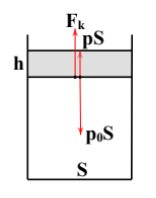
\includegraphics[width=0.25\linewidth]{figs/VN12-Y24-PH-SYL-003P-2}
		\end{center}
		Piston được nâng lên đều nên:
		$$F_k=\left(p_0-p\right)S.$$
		Công cần thực hiện:
		$$A=F_k\Delta h=\left(p_0-p\right)S\Delta h=p_0S\Delta h-A_\text{khí}=\SI{2.6325}{\joule}.$$}
\end{ex}
	\Closesolutionfile{ans}
\subsection{TRẮC NGHIỆM ĐÚNG/SAI}
\setcounter{ex}{0}
\begin{ex}
	Trong quá trình nóng chảy của vật rắn
	\begin{enumerate}[label=\alph*)]
		\item Nhiệt được truyền vào vật rắn để làm tăng nhiệt độ của nó.
		\item Động năng trung bình của các phân tử trong vật rắn giảm đi.
		\item Nội năng của vật rắn không thay đổi.
		\item Tại nhiệt độ nóng chảy, nội năng không thay đổi.
	\end{enumerate}
\loigiai{
\begin{enumerate}[label=\alph*)]
	\item Đúng.
	\item Sai. Động năng trung bình của các phân tử trong vật rắn tăng lên.
	\item Sai. Nội năng của vật rắn thay đổi.
	\item Đúng. Nội năng không thay đổi tại nhiệt độ nóng chảy, vì năng lượng được sử dụng để làm tan chảy các liên kết giữa các phân tử mà không làm thay đổi nhiệt độ.
\end{enumerate}
}
	\end{ex}
% ====================================================================================
\begin{ex}
	Bố trí thí nghiệm như hình bên. Dùng đèn cồn đun nóng ống nghiệm cho đến khi nút bấc bật ra.
	\begin{center}
		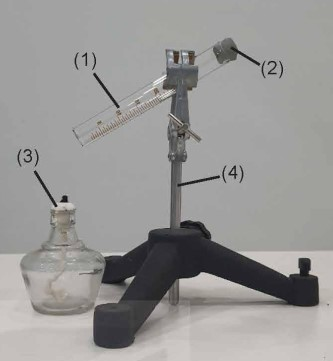
\includegraphics[width=0.3\linewidth]{figs/VN12-Y24-PH-SYL-003P-5}
	\end{center}
	\begin{enumerate}[label=\alph*)]
		\item Khi nút chưa bị bật ra, nội năng của không khí trong ống nghiệm không thay đổi.
		\item Nội năng của không khí trong ống nghiệm tăng không chỉ do động năng chuyển động nhiệt của các phân tử khí tăng mà còn do thế năng tương tác giữa chúng tăng.
		\item Nút bấc bị ra là kết quả của áp suất bên trong ống nghiệm giảm đi.
		\item Quá trình nút bấc bật ra ngoài thì khí trong ống đang thực hiện công.
	\end{enumerate}
\loigiai{
\begin{enumerate}[label=\alph*)]
	\item Sai. Nội năng khí trong ống tăng do nhận nhiệt.
	\item Sai. Thế năng tương tác giữa các phân tử phụ thuộc khoảng cách giữa các phân tử, không phụ thuộc vào nhiệt độ.
	\item Sai. Nút bấc bị ra là kết quả của áp suất bên trong ống nghiệm tăng lên.
	\item Đúng.
\end{enumerate}
}
	\end{ex}

% ====================================================================================
\begin{ex}
		Khối khí được chứa trong cylanh, bên trên được nút kín bằng piston cách nhiệt như hình bên dưới. Dùng tay ấn mạnh piston đồng thời nung nóng bên dưới cylanh bằng ngọn lửa đèn cồn.
	\begin{center}
		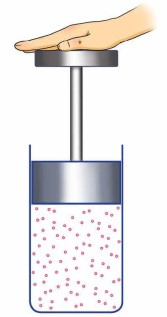
\includegraphics[width=0.15\linewidth]{figs/VN12-Y24-PH-SYL-003P-3}
	\end{center}
	\begin{enumerate}[label=\alph*)]
		\item $A>0$ vì khí nhận công (khí bị nén).
		\item $Q<0$ vì khí bị nung nóng.
		\item Nội năng của khí trong cylanh tăng.
		\item Động năng chuyển động nhiệt của các phân tử khí giảm.
	\end{enumerate}
\loigiai{
\begin{enumerate}[label=\alph*)]
	\item Đúng.
	\item Sai. Khí nhận nhiệt nên $Q>0$.
	\item Đúng.
	\item Sai. Động năng chuyển động nhiệt của các phân tử khí tăng.
\end{enumerate}
}
	

	\end{ex}

% =================================================================================
\begin{ex}
	Khi kéo đi kéo lại sợi dây cuốn quanh một ống nhôm đựng nước nút kín, người ta thấy nước trong ống nóng lên rồi sôi, hơi nước đẩy nút bật ra cùng một lớp hơi nước trắng do các hạt nước rất nhỏ tạo thành.
	\begin{center}
		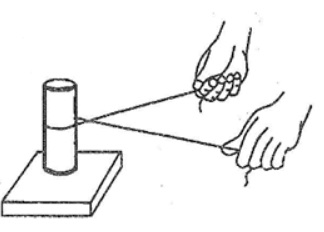
\includegraphics[width=0.3\linewidth]{figs/VN12-Y24-PH-SYL-003P-4}
	\end{center}
	\begin{enumerate}[label=\alph*)]
		\item Ống nhôm nóng lên (nội năng ông nhôm tăng) do nhận công.
		\item Có sự truyền nhiệt từ ống nhôm vào nước, làm cho nước nóng lên và hoá hơi.
		\item Quá trình hơi nước làm bật nút là quá trình hơi nước thực hiện công.
		\item Nếu thay nước bằng rượu thì nút sẽ lâu bật ra hơn.
	\end{enumerate}
\loigiai{
\begin{enumerate}[label=\alph*)]
	\item Đúng.
	\item Đúng.
	\item Đúng.
	\item Sai. Nhiệt độ sôi của rượu thấp hơn nước nên rượu dễ hoá hơi hơn. Quá trình làm nút bật ra sẽ diễn ra nhanh hơn.
\end{enumerate}
}
	\end{ex}

% ====================================================================================
\begin{ex}
	Hằng ngày, Mặt Trời truyền về Trái Đất dưới hình thức bức xạ nhiệt một lượng năng lượng khổng lồ, lớn gấp khoảng 20 000 lần tổng năng lượng mà con người sử dụng. 
	\begin{center}
		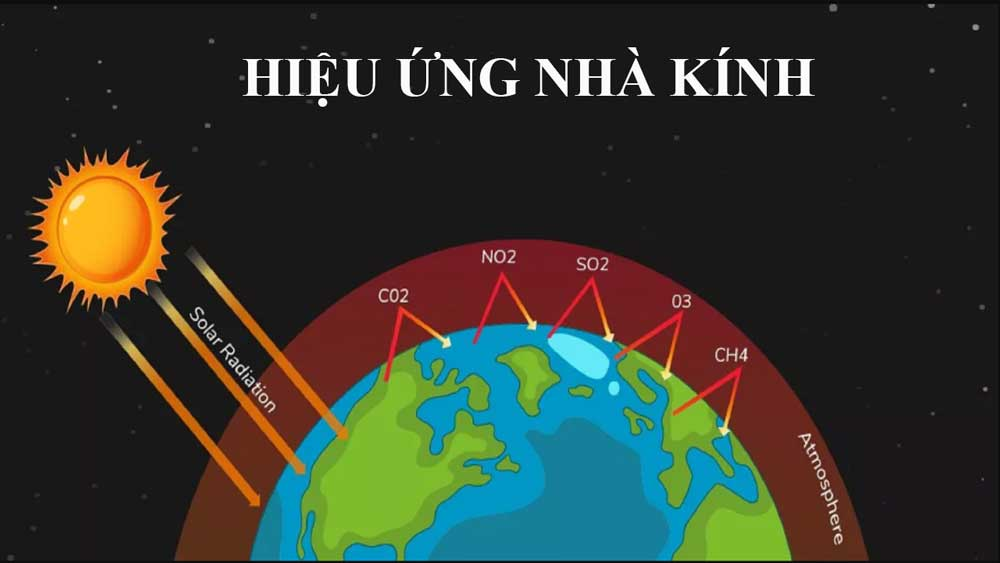
\includegraphics[width=0.45\linewidth]{figs/VN12-Y24-PH-SYL-003P-6}
	\end{center}
	Trái Đất hấp thụ một phần năng lượng này, đồng thời phản xạ lại một phần dưới hình thức bức xạ nhiệt của Trái Đất. Bầu khí quyển bao quanh Trái Đất có tác dụng giống như một nhà lợp kính, giữ lại bức xạ nhiệt của Trái Đất làm cho bề mặt của Trái Đất và không khí bao quanh Trái Đất bị nóng lên. Do sự tương tự đó mà hiệu ứng này của bầu khí quyền được gọi là hiệu ứng nhà kính khí quyển, gọi tắt là hiệu ứng nhà kính.\\
	Trong khí quyển thì khí carbon dioxide $\left(\ce{CO_2}\right)$ đóng vai trò chủ yếu trong việc gây ra hiệu ứng nhà kính. Hiệu ứng nhà kính vừa có thể có ích vừa có thể có hại. Hiện nay, người ta đang cố gắng làm giảm hiệu ứng nhà kính để ngăn không cho nhiệt độ trên Trái Đất tăng lên quá nhanh, làm đe doạ cuộc sống của con người và các sinh vật khác trên hành tinh này.\\
	Nhận định các phát biểu sau đây: 
	\begin{enumerate}[label=\alph*)]
		\item Khí nhà kính có vai trò giữ cho nhiệt độ trên Trái Đất không quá lạnh.
		\item Tăng sử dụng động cơ đốt trong có thể làm giảm hiệu ứng nhà kính.
		\item Một phần nguyên nhân của nước biển dâng là do nhiệt độ trên Trái Đất tăng làm cho nước biển bốc hơi nhiều và gây ra mưa nhiều.
		\item Hiệu ứng nhà kính giúp điều hòa nhiệt độ trên Trái Đất, giúp giảm hạn hán và lũ lụt, giảm băng tan trên địa cực và nước biển dâng cao.
	\end{enumerate}
\loigiai{
\begin{enumerate}[label=\alph*)]
	\item Đúng.
	\item Sai.
	\item Sai.
	\item Sai.
\end{enumerate}
}
	\end{ex}

\subsection{BÀI TẬP TỰ LUẬN}
\setcounter{ex}{0}
\begin{ex}
		Khi đang đóng đinh vào gỗ, mũ đinh có nóng lên nhưng rất ít. Khi đinh đã đóng chắc vào gỗ rồi (không lún thêm được nữa), chỉ cần đóng thêm vài nhát búa là mũ đinh nóng lên rất nhiều. Hãy giải thích?
		\loigiai{
		Khi đang đóng đinh, công thực hiện chuyển thành động năng cho đinh và nội năng cho đinh và búa. Nhưng khi đinh đã được đóng chặt vào gỗ, công thực hiện chỉ chuyển thành nội năng, do đó làm đinh nóng lên nhanh hơn.
	}
	\end{ex}
% ====================================================================================
\begin{ex}
	\immini{
	Hiện nay, kính cường lực (kính chịu lực rất tốt) thường được sử dụng để làm một phần tường của các toà nhà, trung tâm thương mại, \dots thay thế vật liệu gạch, bê tông.\\
	Tuy nhiên, vào những ngày nắng nóng, nếu bước vào những căn phòng có tường làm bằng kính cường lực bị đóng kín, ta thường thấy không khí trong phòng nóng hơn so với bên ngoài.
	\begin{enumerate}[label=\alph*)]
		\item Tại sao không khí trong phòng nóng hơn so với không khí ngoài trời?
		\item Hãy đề xuất các biện pháp đơn giản để làm giảm sự tăng nhiệt của không khí trong phòng vào những ngày mùa hè.
	\end{enumerate}
}{	
\includegraphics[scale=0.3]{figs/VN12-Y24-PH-SYL-003P-1}
}
\loigiai{
\begin{enumerate}[label=\alph*)]
	\item Vào mùa hè, do mặt trời chiếu sáng, không khí trong phòng nhận nhiệt lượng $\left(Q>0\right)$. Do phòng đóng kín nên thể tích khí không đổi, khối khí không sinh công $\left(A=0\right)$. Theo định luật I nhiệt động lực học: $\Delta U=Q+A>0$, nên nội năng của khối khí tăng, làm nhiệt độ không khí trong phòng tăng. Do đó, không khí trong phòng nóng hơn ngoài trời.
	\item Biện pháp đơn giản làm giảm sự tăng nhiệt độ của không khí trong phòng:
	\begin{itemize}
		\item Mở cửa để không khí đối lưu với bên ngoài, từ đó làm nội năng của không khí trong phòng giảm và nhiệt độ phòng giảm xuống.
		\item Lắp rèm cửa: Rèm thường bằng vải dày chuyên dụng, màu sẫm, bề mặt lượn sóng. Khi ánh sáng mặt trời đi qua rèm nó vừa bị phản xạ (do bề mặt, do chất liệu vải), vừa bị hấp thụ (do màu sắc, độ dày của vải). Bên cạnh đó, giữa rèm và mặt kính có có một khoảng ngăn cách, lớp không khí này có khả năng ngăn một phần sự truyền nhiệt từ bên ngoài vào phòng (do không khí dẫn nhiệt kém). Các yếu tố trên làm hạn chế khả năng truyền nhiệt trực tiếp từ Mặt Trời vào sâu bên trong phòng, làm nhiệt độ trong phòng tăng chậm hơn.
		\item Dán tấm phim cách nhiệt: Phim cách nhiệt thường có cấu tạo đặc biệt (từ nhiều lớp polyester và chống ánh sáng tử ngoại), nên khi ánh sáng mặt trời chiếu vào, tấm phim cách nhiệt vừa có tác dụng phản xạ (chủ yếu với ánh sáng hồng ngoại), vừa có tác dụng hấp thụ ánh sáng (chủ yếu với ánh sáng tử ngoại) và truyền qua với các ánh sáng dịu với mắt.
	\end{itemize}
\end{enumerate}
}
	\end{ex}
% ====================================================================================
\begin{ex}
	Thực hiện công $\SI{150}{\joule}$ để nén khí trong một cylanh thì khí truyền ra môi trường xung quanh nhiệt lượng $\SI{30}{\joule}$. Xác định độ thay đổi nội năng của khí trong cylanh.
	\loigiai{
	Khí nhận công nên $A>0\Rightarrow A=\SI{150}{\joule}$, khí truyền nhiệt nên $Q<0\Rightarrow Q=\SI{-30}{\joule}$.\\
	Độ biến thiên nội năng của khí:
	$$\Delta U=Q+A=\SI{120}{\joule}.$$
}
	\end{ex}

% ====================================================================================
\begin{ex}
	Giả sử một người đang thực hiện bài vận động vất vả chẳng hạn như nâng tạ hoặc đạp xe. Cơ thể đang thực hiện công và đồng thời nhiệt lượng thoát ra ngoài qua lỗ chân lông vào không khí xung quanh. Theo định luật I nhiệt động lực học, nhiệt độ cơ thể sẽ giảm dần trong quá trình tập luyện. Tuy nhiên, điều đó lại không xảy ra. Như vậy, có phải định luật I nhiệt động lực học không đúng trong trường hợp này phải không? Hãy giải thích.
	\loigiai{
	Trong quá trình vận động cơ thể con người thực hiện công và toả nhiệt ra ngoài môi trường nhưng trong cơ thể người luôn có năng lượng dự trữ để cung cấp năng cho các hoạt động của cơ thể. Năng lượng dự trữ này có được do các quá trình biến đổi chất dinh dưỡng từ thức ăn. Vì vậy, cơ thể luôn được duy trì ở nhiệt độ ổn định và định luật I nhiệt động lực học trong trường hợp này vẫn được nghiệm đúng.
}
	\end{ex}

% ===================================================================================
\begin{ex}
	Một quả bóng khối lượng $\SI{200}{\gram}$ rơi từ độ cao $\SI{15}{\meter}$ xuống sân và nảy lên được $\SI{10}{\meter}$. Độ biến thiên nội năng của quả bóng là bao nhiêu? Lấy $g=\SI{10}{\meter/\second^2}$.
	\loigiai{
	Độ biến thiên nội năng của quả bóng:
	$$\Delta U=mg\left(h-h'\right)=\SI{10}{\joule}.$$
}
\end{ex}

% ===================================================================================
\begin{ex}
	Một vật khối lượng $\SI{1}{\kilogram}$ trượt không vận tốc đầu từ đỉnh xuống chân một mặt phẳng dài $\SI{21}{\meter}$, nghiêng $\SI{30}{\degree}$ so với mặt nằm ngang. Tốc độ của vật ở chân mặt phẳng nghiêng là $\SI{4.1}{\meter/\second}$. Tính công của lực ma sát và độ biến thiên nội năng của vật trong quá trình chuyển động trên. Lấy $g=\SI{9.8}{\meter/\second^2}$. Bỏ qua sự trao đổi nhiệt với mặt phẳng nghiêng.
	\loigiai{
		Công của lực ma sát:
		$$A_\text{ms}=W_\text{s}-W_\text{t}=mgh_\text{s}+\dfrac{1}{2}mv^2_\text{s}-mgh_\text{t}-\dfrac{1}{2}mv^2_\text{t}=\dfrac{1}{2}mv^2_\text{s}-mg\ell\sin\SI{30}{\degree}\approx\SI{-94.5}{\joule}.$$
		Độ biến thiên nội năng của vật trong quá trình chuyển động bằng công của lực ma sát:
		$$\Delta U=\SI{94.5}{\joule}.$$
	}
\end{ex}
	
\newpage\section{NHIỆT DUNG RIÊNG}
\subsection{LÝ THUYẾT TRỌNG TÂM}
\subsubsection{Nhiệt dung riêng}
\begin{boxdn}
	Nhiệt dung riêng của một chất là nhiệt lượng cần cung cấp để nhiệt độ của $\SI{1}{\kilogram}$ chất đó tăng thêm $\SI{1}{\kelvin}$.
\end{boxdn}
Đơn vị đo của nhiệt dung riêng trong hệ SI là $\si{\joule/\left(\kilogram\cdot\kelvin\right)}$, nhiệt dung riêng kí hiệu là $c$.
\subsubsection{Nhiệt lượng trao đổi để khối chất thay đổi nhiệt độ}
\begin{boxdn}
	Nhiệt lượng trao đổi (toả ra hay nhận vào) để khối chất thay đổi nhiệt độ từ $T_1$ đến nhiệt độ $T_2$:
	$$Q=mc\Delta T$$
\end{boxdn}
với:
\begin{itemize}
	\item $Q$: nhiệt lượng trao đổi, đơn vị trong hệ SI là $\si{\joule}$;
	\item $m$: khối lượng, đơn vị trong hệ SI là $\si{\kilogram}$;
	\item $c$: nhiệt dung riêng của chất tạo nên vật, đơn vị trong hệ SI là $\si{\joule/\left(\kilogram\cdot\kelvin\right)}$;
	\item $\Delta T=T_2-T_1$: độ biến thiên nhiệt độ, đơn vị trong hệ SI là $\si{\kelvin}$.
\end{itemize}
\subsubsection{Trạng thái cân bằng nhiệt của hệ nhiệt động}
\begin{boxdn}
	Hệ nhiệt động đạt trạng thái cân bằng nhiệt khi tổng nhiệt lượng trao đổi trong hệ bằng 0:
	$$\sum Q=Q_1+Q_2+\dots+Q_n=0.$$
\end{boxdn}
\subsection{VÍ DỤ MINH HOẠ}
\begin{dang}{Xác định nhiệt lượng trao đổi để khối chất thay đổi nhiệt độ}
	\end{dang}
	\begin{vd}
		Hãy giải thích tại sao ban ngày có gió mát thổi từ biển vào đất liền? Biết rằng nhiệt dung riêng của đất và nước vào khoảng $\SI{800}{\joule/\left(\kilogram\cdot\kelvin\right)}$ và $\SI{4200}{\joule/\left(\kilogram\cdot\kelvin\right)}$.
	\loigiai{Vào ban ngày, vì nhiệt dung riêng của nước cao hơn nhiệt dung riêng của đất nên với cùng nhiệt lượng nhận từ Mặt Trời thì nước biển có độ tăng nhiệt độ thấp hơn đất liền. Do hiện tượng đối lưu, luồng không khí từ biển sẽ thổi vào đất liền. Lúc này có sự trao đổi nhiệt lượng giữa không khí trong đất liền và không khí từ biển thổi vào làm giảm nhiệt độ không khí ở đất liền. Do đó, chúng ta sẽ cảm thấy mát hơn}

	\end{vd}
	
	
\begin{vd}
Một thùng đựng $\SI{20}{\ell}$ nước ở nhiệt độ $\SI{20}{\celsius}$. Cho khối lượng riêng của nước là $\SI{1000}{\kilogram\cdot\meter^{-3}}$, nhiệt dung riêng của nước $c=\SI{4200}{\joule/\left(\kilogram\cdot\kelvin\right)}$.
			\begin{enumerate}[label=\alph*)]
				\item Tính nhiệt lượng cần truyền cho nước trong thùng để nhiệt độ của nó tăng lên tới $\SI{70}{\celsius}$.
				\item Tính thời gian truyền nhiệt lượng cần thiết nếu dùng một thiết bị điện có công suất $\SI{2.5}{\kilo\watt}$ để đun lượng nước trên. Biết chỉ có $\SI{80}{\percent}$ điện năng tiêu thụ được dùng để làm nóng nước.
			\end{enumerate}
	\loigiai{
				\begin{enumerate}[label=\alph*)]
					\item Khối lượng của $\SI{20}{\ell}$ nước:
					$$m=\rho V=\left(\SI{1000}{\kilogram\cdot\meter^{-3}}\right)\cdot\left(\SI{20E-3}{\meter^{3}}\right)=\SI{20}{\kilogram}.$$
					Nhiệt lượng cần truyền cho nước trong thùng để nhiệt độ của nó tăng lên tới $\SI{70}{\celsius}$:
					$$Q=mc\Delta t=\left(\SI{20}{\kilogram}\right)\cdot\left[\SI{4200}{\joule/\left(\kilogram\cdot\kelvin\right)}\right]\cdot\left(\SI{50}{\kelvin}\right)=\SI{42E5}{\joule}.$$
					\item Năng lượng thiết bị điện tiêu thụ để truyền được nhiệt lượng cần thiết đun nóng nước đến $\SI{70}{\celsius}$:
					$$W=\dfrac{Q}{H}=\SI{52.5E5}{\joule}.$$
					Thời gian đun nước:
					$$t=\dfrac{W}{\calP}=\dfrac{\SI{52.5E5}{\joule}}{\SI{2.5E3}{\watt}}=\SI{2100}{\second}=\SI{35}{\minute}.$$
				\end{enumerate}}
		
\end{vd}
\begin{dang}{Vận dụng phương trình cân bằng nhiệt}
	\end{dang}
\begin{vd}
		Một bác thợ rèn nhúng một con dao rựa bằng thép có khối lượng $\SI{1.1}{\kilogram}$ ở nhiệt độ $\SI{850}{\celsius}$ vào trong bể nước lạnh để làm tăng độ cứng của lưỡi dao. Nước trong bể có thể tích $\SI{200}{\ell}$ và có nhiệt độ bằng nhiệt độ ngoài trời là $\SI{27}{\celsius}$. Xác định nhiệt độ của nước khi có sự cân bằng nhiệt. Bỏ qua sự truyền nhiệt cho thành bể, môi trường bên ngoài và bỏ qua quá trình nước hoá hơi khi vừa tiếp xúc với rựa. Biết nhiệt dung riêng của thép là $\SI{460}{\joule/\left(\kilogram\cdot\kelvin\right)}$; của nước là $\SI{4180}{\joule/\left(\kilogram\cdot\kelvin\right)}$.
\loigiai{
			Gọi $t_\text{cb}$ là nhiệt độ của nước khi có sự cân bằng nhiệt.\\
			Hệ đạt trạng thái cân bằng nhiệt khi tổng nhiệt lượng trao đổi trong hệ bằng 0:
			\begin{eqnarray*}
				&&	Q_\text{rựa}+Q_\text{nước}=0\\
				&\Leftrightarrow&	m_\text{t}c_\text{t}\left(t_\text{cb}-t_\text{t}\right)+m_\text{n}c_\text{n}\left(t_\text{cb}-t_\text{n}\right)=0\\
				&\Rightarrow& t_\text{cb}=\dfrac{m_\text{n}c_\text{n}t_\text{n}+m_\text{t}c_\text{t}t_\text{t}}{m_\text{n}c_\text{n}+m_\text{t}c_\text{t}}\approx\SI{27.5}{\celsius}.
			\end{eqnarray*}
		}
\end{vd}
	
\begin{vd}
Một bình nhiệt lượng kế bằng nhôm có khối lượng $m_1=\SI{200}{\gram}$ chứa $m_2=\SI{400}{\gram}$ nước ở nhiệt độ $t_1=\SI{20}{\celsius}$. Đổ thêm vào bình một khối lượng nước $m$ ở nhiệt độ $t_2=\SI{5}{\celsius}$. Khi cân bằng nhiệt thì nhiệt độ của nước trong bình là $t=\SI{10}{\celsius}$. Cho biết nhiệt dung riêng của nhôm là $c_1=\SI{880}{\joule/\left(\kilogram\cdot\kelvin\right)}$, của nước là $c_2=\SI{4200}{\joule/\left(\kilogram\cdot\kelvin\right)}$. Bỏ qua sự trao đổi nhiệt với môi trường. Xác định giá trị của $m$.
\loigiai{Khi hệ đạt trạng thái cân bằng nhiệt thì tổng nhiệt lượng trao đổi của hệ bằng 0:
			$$mc_2\left(t-t_2\right)+m_1c_1\left(t-t_1\right)+m_2c_2\left(t-t_1\right)=0$$
			\begin{eqnarray*}
				\Rightarrow m&=&\dfrac{m_1c_1\left(t-t_1\right)+m_2c_2\left(t-t_1\right)}{c_2\left(t_2-t\right)}\\
				&=&\dfrac{\left\{\left(\SI{0.2}{\kilogram}\right)\cdot\left[\SI{880}{\joule/\left(\kilogram\cdot\kelvin\right)}\right]+\left(\SI{0.4}{\kilogram}\right)\cdot\left[\SI{4200}{\joule/\left(\kilogram\cdot\kelvin\right)}\right]\right\}\cdot\left(\SI{10}{\celsius}-\SI{20}{\celsius}\right)}{\left[\SI{4200}{\joule/\left(\kilogram\cdot\kelvin\right)}\right]\cdot\left(\SI{5}{\celsius}-\SI{10}{\celsius}\right)}\\
				&\approx&\SI{0.88}{\kilogram}.
			\end{eqnarray*}
		}
\end{vd}
\subsection{BÀI TẬP TRẮC NGHIỆM}
\setcounter{ex}{0}
\Opensolutionfile{ans}[ans/G12Y24B4TN]
% ===================================================================
\begin{ex}
	Nhiệt lượng vật trao đổi để thay đổi nhiệt độ phụ thuộc vào
	\choice
	{khối lượng, thể tích và độ thay đổi nhiệt độ của vật}
	{ thể tích, nhiệt độ ban đầu và chất cấu tạo nên vật}
	{\True  khối lượng của vật, chất cấu tạo nên vật và độ thay đổi nhiệt độ của vật}
	{nhiệt độ ban đầu, nhiệt độ lúc sau và áp suất của môi trường}
	\loigiai{ }
	\end{ex}
% ===================================================================
\begin{ex}
	Có 4 bình A, B, C, D đều đựng nước ở cùng một nhiệt độ với thể tích tương ứng là: 1 lít, 2 lít, 3 lít, 4 lít. Sau
	khi dùng các đèn cồn giống hệt nhau để đun các bình này khác nhau. Bình có nhiệt độ thấp nhất là
	\begin{center}
		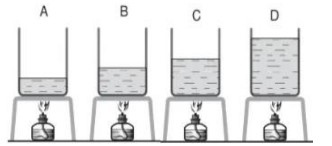
\includegraphics[width=0.4\linewidth]{figs/VN12-Y24-PH-SYL-004P-1}
	\end{center}
	\choice
	{bình A}
	{bình B}
	{bình C}
	{\True bình D}
	\loigiai{}
\end{ex}
% ===================================================================
\begin{ex}
Có 4 bình A, B, C, D đều đựng nước ở cùng một nhiệt độ với thể tích tương ứng là: 1 lít, 2 lít, 3 lít, 4 lít. Sau
khi dùng các đèn cồn giống hệt nhau để đun các bình này khác nhau. Bình có nhiệt độ cao nhất là
\begin{center}
	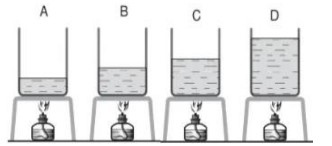
\includegraphics[width=0.4\linewidth]{figs/VN12-Y24-PH-SYL-004P-1}
\end{center}
	\choice
	{\True bình A}
	{bình B}
	{bình C}
	{bình D}
	\loigiai{}
\end{ex}
% ===================================================================
\begin{ex}
	Chọn phát biểu \textbf{sai}.\\
	Nhiệt dung riêng của một chất 
	\choice
	{là nhiệt lượng cần truyền để $\SI{1}{\kilogram}$ chất đó tăng thêm $\SI{1}{\celsius}$}
	{\True phụ thuộc vào khối lượng riêng của chất đó}
	{phụ thuộc vào bản chất của chất đó}
	{có đơn vị là $\si{\joule/\kilogram\cdot\kelvin}$}
	\loigiai{}
\end{ex}
% ===================================================================
\begin{ex}
Nhiệt độ của vật nào tăng lên nhiều nhất khi ta thả rơi bốn vật dưới đây có cùng khối lượng và từ cùng một độ cao xuống đất? Coi như toàn bộ cơ năng của vật chuyển hoá thành nhiệt năng.
	\choice
	{Vật bằng nhôm, có nhiệt dung riêng là $\SI{880}{\joule/\kilogram\cdot\kelvin}$}
	{Vật bằng đồng, có nhiệt dung riêng là $\SI{380}{\joule/\kilogram\cdot\kelvin}$}
	{\True Vật bằng chì, có nhiệt dung riêng là $\SI{120}{\joule/\kilogram\cdot\kelvin}$}
	{Vật bằng gang, có nhiệt dung riêng là $\SI{5500}{\joule/\kilogram\cdot\kelvin}$}
	\loigiai{$$\Delta t=\dfrac{Q}{mc}.$$
		Vì chì có nhiệt dung riêng nhỏ nhất nên có độ tăng nhiệt độ nhiều nhất}
\end{ex}
% ===================================================================
\begin{ex}
	Tính nhiệt lượng do miếng sắt khối lượng $\SI{2}{\kilogram}$ toả ra khi hạ nhiệt độ từ $\SI{500}{\celsius}$ xuống còn $\SI{40}{\celsius}$. Biết nhiệt dung riêng của sắt là $\SI{478}{\joule/\left(\kilogram\cdot\kelvin\right)}$
	\choice
	{$\SI{219880}{\joule}$}
	{\True $\SI{439760}{\joule}$}
	{$\SI{879520}{\joule}$}
	{$\SI{109940}{\joule}$}
	\loigiai{
		Nhiệt lượng miếng sắt toả ra:
		$$Q=mc\left(t_1-t_2\right)=\SI{439760}{\joule}.$$	
	}
\end{ex}
% ===================================================================
\begin{ex}
	Một viên đạn bằng bạc đang bay với tốc độ $\SI{200}{\meter/\second}$ thì va chạm vào một bức tường gỗ và nằm yên trong bức tường. Nhiệt dung riêng của bạc là $\SI{234}{\joule/\left(\kilogram\cdot\kelvin\right)}$. Nếu coi viên đạn không trao đổi nhiệt với bên ngoài thì nhiệt độ của viên đạn sẽ tăng thêm bao nhiêu độ?
	\choice
	{$\SI{58}{\celsius}$}
	{$\SI{171}{\celsius}$}
	{\True $\SI{85}{\celsius}$}
	{$\SI{250}{\celsius}$}
	\loigiai{
		Áp dụng định luật bảo toàn và chuyển hoá năng lượng:
		$$\dfrac{1}{2}mv^2=mc\Delta t\Rightarrow \Delta t=\dfrac{v^2}{2c}\approx\SI{85}{\celsius}.$$	
	}
\end{ex}
% ===================================================================
\begin{ex}
	Người ta cọ xát hai vật với nhau, nhiệt dung của hai vật là $\SI{800}{\joule/\kelvin}$. Sau 1 phút người ta thấy nhiệt độ của mỗi vật tăng thêm $\SI{30}{\kelvin}$. Công suất trung bình của việc cọ xát bằng
	\choice
	{$\SI{1080}{\watt}$}
	{$\SI{980}{\watt}$}
	{$\SI{480}{\watt}$}
	{\True $\SI{800}{\watt}$}
	\loigiai{	Công suất trung bình của việc cọ xát là
		$$\calP=\dfrac{2c\Delta T}{t}=\SI{800}{\watt}.$$}
\end{ex}
% ===================================================================
\begin{ex}
	Đầu thép của một búa máy có khối lượng $\SI{12}{\kilogram}$ nóng lên thêm $\SI{20}{\celsius}$ sau 1,5 phút hoạt động. Biết rằng  $\SI{40}{\percent}$ cơ năng của búa máy chuyển thành nhiệt năng của đầu búa. Nhiệt dung riêng của thép là $\SI{460}{\joule/\kilogram\cdot\kelvin}$. Công suất của búa gần nhất với giá trị nào sau đây?
	\choice
	{\True $\SI{3}{\kilo\watt}$}
	{$\SI{4}{\kilo\watt}$}
	{$\SI{5}{\kilo\watt}$}
	{$\SI{6}{\kilo\watt}$}
	\loigiai{		Công suất toả nhiệt trên đầu búa:
		$$\calP_\text{hp}=\dfrac{mc\Delta T}{t}\approx\SI{1226.67}{\watt}.$$
		Công suất của búa:
		$$\calP=\dfrac{\calP_\text{hp}}{0,4}\approx\SI{3.066}{\kilo\watt}.$$}
\end{ex}
% ===================================================================
\begin{ex}
	\immini{Quả cầu kim loại được làm bằng chất có nhiệt dung riêng $c=\SI{460}{\joule/\left(\kilogram\cdot\kelvin\right)}$ được treo bởi sợi day có chiều dài $\ell=\SI{46}{\centi\meter}$. Quả cầu được nâng lên đến B rồi thả rơi. Sau khi chạm tường, nó bật lên đến C $\left(\alpha=\SI{60}{\degree}\right)$. Biết rằng $\SI{60}{\percent}$ độ giảm thế năng của quả cầu biến thành nhiệt làm nóng quả cầu. Lấy $g=\SI{10}{\meter/\second^2}$. Độ tăng nhiệt độ của quả cầu là
\choice
{\True $\SI{3E-3}{\celsius}$}
{$\SI{6E-3}{\celsius}$}
{$\SI{1.5E-3}{\celsius}$}
{Không đủ dữ kiện để xác định}	
}{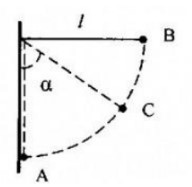
\includegraphics[scale=0.8]{figs/VN12-Y24-PH-SYL-004P-2}
}
	\loigiai{Độ tăng nhiệt độ của quả cầu:
		$$\Delta t=\dfrac{0,6mg\ell\cos\SI{60}{\degree}}{mc}=\dfrac{0,6g\ell\cos\SI{60}{\degree}}{c}=\SI{3E-3}{\celsius}.$$}
\end{ex}
% ===================================================================
\begin{ex}
	Có hai quả cầu bằng chì giống nhau có nhiệt dung riêng là $c$, chuyển động đến va chạm mềm trực diện với tốc độ lần lượt là $v$ và $2v$. Cho rằng toàn bộ cơ năng mất mát trong quá trình va chạm chuyển hoá thành nhiệt năng làm nóng hai quả cầu. Độ tăng nhiệt độ của hai quả cầu là
		\choice
		{\True $\dfrac{9v^2}{8c}$}
		{$\dfrac{7v^2}{8c}$}
		{$\dfrac{9v^2}{7c}$}
		{$\dfrac{11v^2}{7c}$}
	\loigiai{Tốc độ hai quả cầu sau va chạm:
		$$V=\dfrac{2mv-mv}{2m}=0,5v.$$
		Nhiệt lượng toả ra trong quá trình va chạm:
		$$Q=\dfrac{1}{2}mv^2+\dfrac{1}{2}m\left(2v\right)^2-\dfrac{1}{2}\cdot 2mV^2=\dfrac{9}{4}mv^2.$$
		Độ tăng nhiệt độ của hai quả cầu:
		$$\Delta t=\dfrac{Q}{2mc}=\dfrac{9v^2}{8c}.$$}
\end{ex}
% ===================================================================
\begin{ex}
Một lượng nước và một lượng rượu có thể tích bằng nhau, được cung cấp nhiệt lượng tương ứng là $Q_1$ và $Q_2$. Biết khối lượng riêng của nước là $\SI{1000}{\kilogram/\meter^3}$ và của rượu là $\SI{800}{\kilogram/\meter^3}$, nhiệt dung riêng của nước là $\SI{4200}{\joule/\kilogram\cdot\kelvin}$ và của rượu là $\SI{2500}{\joule/\kilogram\cdot\kelvin}$. Để độ tăng nhiệt độ của nước và rượu bằng nhau thì
	\choice
	{$Q_1=Q_2$}
	{$Q_1=1,25Q_2$}
	{$Q_1=1,68Q_2$}
	{\True $Q_1=2,1Q_2$}
	\loigiai{	$$\dfrac{Q_1}{Q_2}=\dfrac{m_1c_1\Delta t}{m_2c_2\Delta t}=\dfrac{D_1c_1}{D_2c_2}=2,1.$$}
\end{ex}
% ===================================================================
\begin{ex}
	Một ấm đồng khối lượng $\SI{300}{\gram}$ chứa 1 lít nước ở nhiệt độ $\SI{15}{\celsius}$. Biết trung bình mỗi giây bếp truyền cho ấm một nhiệt lượng là $\SI{500}{\joule}$. Bỏ qua sự hao phí về nhiệt ra môi trường xung quanh. Lấy nhiệt dung riêng của đồng là $\SI{380}{\joule/\kilogram\cdot\kelvin}$ và của nước là $\SI{4186}{\joule/\kilogram\cdot\kelvin}$. Thời gian đun sôi ấm nước có giá trị gần đúng là
	\choice
	{\True 12 phút}
	{13 phút}
	{14 phút}
	{15 phút}
	\loigiai{Nhiệt lượng nước và ấm cần thu vào để sôi:
		$$Q=\left(m_1c_1+m_2c_2\right)\Delta t=\SI{365500}{\joule}.$$
		Thời gian đun sôi ấm nước:
		$$t=\dfrac{Q}{\SI{500}{\joule/\second}}=\SI{731}{\second}\approx\SI{12}{\text{phút}}.$$}
\end{ex}
% ===================================================================
\begin{ex}
	Người ta muốn pha nước tắm với nhiệt độ $\SI{38}{\celsius}$ thì phải pha bao nhiêu lít nước sôi vào 15 lít nước lạnh ở $\SI{24}{\celsius}$?
	\choice
	{2,5 lít}
	{\True 3,38 lít}
	{4,2 lít}
	{5 lít}
	\loigiai{$$Q_1+Q_2=0\Leftrightarrow V_1\rho c\left(t_\text{cb}-t_1\right)+V_2\rho c\left(t_\text{cb}-t_2\right)=0$$
		$$\Leftrightarrow V_1\left(38-100\right)+15\cdot\left(38-24\right)=0\Rightarrow V_1=\SI{3.38}{\liter}.$$}
\end{ex}
% ===================================================================
\begin{ex}
	Một ấm đun nước bằng nhôm có khối lượng $\SI{400}{\gram}$, chứa 3 lít nước được đun trên bếp. Khi nhận thêm nhiệt lượng $\SI{740}{\kilo\joule}$ thì ấm đạt đến nhiệt độ $\SI{80}{\celsius}$. Biết nhiệt dung riêng của nhôm và nước lần lượt là $c_1=\SI{880}{\joule/\left(\kilogram\cdot\kelvin\right)}$, $c_2=\SI{4190}{\joule/\left(\kilogram\cdot\kelvin\right)}$. Nhiệt độ ban đầu của ấm là
	\choice
	{$\SI{8.15}{\celsius}$}
	{$\SI{8.15}{\kelvin}$}
	{\True $\SI{22.7}{\celsius}$}
	{$\SI{22.7}{\kelvin}$}
	\loigiai{$$Q=\left(m_1c_1+m_2c_2\right)\Delta t\Rightarrow \Delta t=\dfrac{Q}{m_1c_1+m_2c_2}\approx\SI{57.27}{\celsius}.$$
		Nhiệt độ ban đầu của ấm:
		$$t_1=t_2-\Delta t=\SI{22.73}{\celsius}.$$}
\end{ex}
% ===================================================================
\begin{ex}
Thả một miếng thép $\SI{2}{\kilogram}$ đang ở nhiệt độ $\SI{345}{\celsius}$ vào một bình đựng 3 lít nước. Sau khi cân bằng nhiệt, nhiệt độ cuối cùng của nước là $\SI{30}{\celsius}$. Bỏ qua sự trao đổi nhiệt với môi trường. Nhiệt dung riêng của thép và nước lần lượt là $\SI{460}{\joule/\kilogram\cdot\kelvin}$, $\SI{4200}{\joule/\kilogram\cdot\kelvin}$. Nhiệt độ ban đầu của nước là
	\choice
	{\True $\SI{7}{\celsius}$}
	{$\SI{17}{\celsius}$}
	{$\SI{27}{\celsius}$}
	{$\SI{37}{\celsius}$}
	\loigiai{Khi hệ đạt trạng thái cân bằng nhiệt thì tổng nhiệt lượng trao đổi trong hệ bằng 0:
		$$m_1c_1\left(t-t_1\right)+m_2c_2\left(t-t_2\right)=0$$
		$$\Leftrightarrow 2\cdot460\cdot\left(\SI{30}{\celsius}-\SI{345}{\celsius}\right)+3\cdot 4200\left(\SI{30}{\celsius}-t_2\right)=0\Rightarrow t_2=\SI{7}{\celsius}.$$}
\end{ex}
% ===================================================================
\begin{ex}
Thả một quả cầu nhôm khối lượng $\SI{0.15}{\kilogram}$ được đun nóng tới $\SI{100}{\celsius}$ vào một cốc nước ở $\SI{20}{\celsius}$. Sau một thời gian, nhiệt độ của quả và nước đều bằng $\SI{25}{\celsius}$. Coi quả cầu và nước chỉ trao đổi nhiệt cho nhau và bỏ qua quá trình nước hoá hơi khi tiếp xúc với bề mặt quả cầu. Cho nhiệt dung riêng của nhôm và nước lần lượt là $\SI{800}{\joule/\kilogram\cdot\kelvin}$, $\SI{4200}{\joule/\kilogram\cdot\kelvin}$. Khối lượng của nước là 
	\choice
	{$\SI{0.47}{\gram}$}
	{\True $\SI{0.43}{\kilo\gram}$}
	{$\SI{2}{\gram}$}
	{$\SI{2}{\kilo\gram}$}
	\loigiai{Khi cân bằng nhiệt, tổng nhiệt lượng trao đổi trong hệ bằng 0:
		$$m_1c_1\left(t-t_1\right)+m_2c_2\left(t-t_2\right)=0\Rightarrow m_2=\SI{0.4285}{\kilogram}.$$}
\end{ex}

% ===================================================================
\begin{ex}
	Thả một quả cầu bằng nhôm có khối lượng $\SI{0.21}{\kilogram}$ được nung nóng đến $\SI{200}{\celsius}$ vào cốc đựng nước ở $\SI{30}{\celsius}$. Sau một thời gian, nhiệt độ của nước và quả cầu đều bằng $\SI{50}{\celsius}$. Biết nhiệt dung riêng của nhôm là $\SI{880}{\joule/\left(\kilogram\cdot\kelvin\right)}$, nhiệt dung riêng của nước là $\SI{4200}{\joule/\left(\kilogram\cdot\kelvin\right)}$. Khối lượng nước trong cốc là	
	\choice
	{$\SI{3.3}{\kilogram}$}
	{$\SI{7.5}{\kilogram}$}
	{$\SI{0.21}{\kilogram}$}
	{\True $\SI{0.33}{\kilogram}$}
	\loigiai{
		Áp dụng phương trình cân bằng nhiệt:
		$$m_1c_1\left(t_\text{cb}-t_1\right)+m_2c_2\left(t_\text{cb}-t_2\right)=0$$
		$$\Rightarrow m_2=\dfrac{m_1c_1\left(t_\text{cb}-t_1\right)}{c_2\left(t_2-t_\text{cb}\right)}=\SI{0.33}{\kilogram}.$$ }
	
\end{ex}
% ===================================================================
\begin{ex}
	Người ta thả một miếng đồng có khối lượng $m_1=\SI{0.2}{\kilogram}$ được đốt nóng đến nhiệt độ $t_1$ vào một nhiệt lượng kế chứa $m_2=\SI{0.28}{\kilogram}$ nước ở nhiệt độ $t_2=\SI{20}{\celsius}$. Nhiệt độ khi có cân bằng nhiệt là $t_3=\SI{80}{\celsius}$. Biết nhiệt dung riêng của đồng và nước lần lượt là $c_1=\SI{400}{\joule/\left(\kilogram\cdot\kelvin\right)}$, $c_2=\SI{4200}{\joule/\left(\kilogram\cdot\kelvin\right)}$. Bỏ qua sự trao đổi nhiệt với nhiệt lượng kế và với môi trường. Nhiệt độ ban đầu $t_1$ của đồng là
	\choice
	{$\SI{926}{\celsius}$}
	{\True $\SI{962}{\celsius}$}
	{$\SI{530}{\celsius}$}
	{$\SI{503}{\celsius}$}
	\loigiai{
		Áp dụng phương trình cân bằng nhiệt:
		$$m_1c_1\left(t_3-t_1\right)+m_2c_2\left(t_3-t_2\right)=0\Rightarrow t_1=\SI{962}{\celsius}.$$
	}
\end{ex}
% ===================================================================
\begin{ex}
	Một bình nhiệt lượng kế bằng thép khối lượng $\SI{0.1}{\kilogram}$ chứa $\SI{0.5}{\kilogram}$ nước ở nhiệt độ $\SI{15}{\celsius}$. Người ta thả một miếng chì và một miếng nhôm có tổng khối lượng $\SI{0.15}{\kilogram}$ và nhiệt độ $\SI{100}{\celsius}$ vào nhiệt lượng kế. Kết quả là nhiệt độ của nước trong nhiệt lượng kế tăng lên đến $\SI{17}{\celsius}$. Cho biết nhiệt dung riêng của chì là $\SI{127.7}{\joule/\left(
		\kilogram\cdot\kelvin\right)}$, của nhôm là $\SI{836}{\joule/\left(\kilogram\cdot\kelvin\right)}$, của thép là $\SI{460}{\joule/\left(\kelvin\cdot\kelvin\right)}$, của nước là $\SI{4180}{\joule/\left(\kilogram\cdot\kelvin\right)}$. Bỏ qua sự mất mát nhiệt ra bên ngoài. Khối lượng của miếng chì và miếng nhôm lần lượt \textbf{gần với giá trị nào nhất} sau đây?
	\choice
	{$\SI{46}{\gram}$ và $\SI{104}{\gram}$}
	{$\SI{110}{\gram}$ và $\SI{40}{\gram}$}
	{\True $\SI{104}{\gram}$ và $\SI{46}{\gram}$}
	{$\SI{40}{\gram}$ và $\SI{110}{\gram}$}
	\loigiai{
		Ta có:
		\begin{equation}
			m_{\ce{Pb}}+m_{\ce{Al}}=\SI{0.15}{\kilogram}
			\label{eq:D1-1}
		\end{equation}	
		Áp dụng phương trình cân bằng nhiệt:
		$$m_{\ce{Pb}}c_{\ce{Pb}}\left(t_\text{cb}-t_{\ce{Pb}}\right)+m_{\ce{Al}}c_{\ce{Al}}\left(t_\text{cb}-t_{\ce{Al}}\right)+m_\text{nlk}c_\text{nlk}\left(t_\text{cb}-t_\text{nlk}\right)+m_\text{n}c_\text{n}\left(t_\text{cb}-t_\text{n}\right)=0.$$
		\begin{equation}
			\Rightarrow 10599,1m_{\ce{Pb}}+69388m_{\ce{Al}}=4272
			\label{eq:D1-2}
		\end{equation}
		Từ (\ref{eq:D1-1}) và (\ref{eq:D1-2}), thu được:
		$\heva{
			m_{\ce{Pb}}\approx\SI{104}{\gram}\\
			m_{\ce{Al}}\approx\SI{46}{\gram}
		}$.
	}
\end{ex}

% ===================================================================
\begin{ex}
	Một nhiệt lượng kế bằng nhôm có khối lượng $m$ ở nhiệt độ $t_1=\SI{20}{\celsius}$. Cho vào nhiệt lượng kế một lượng nước có khối lượng $m$ ở nhiệt độ $t_2$. Khi có cân bằng nhiệt, nhiệt độ của nước giảm đi $\SI{12}{\celsius}$. Tiếp tục đổ thêm một chất lỏng khác có khối lượng $2m$ ở nhiệt độ $t_3=\SI{40}{\celsius}$ (chất lỏng này không tác dụng hoá học với nước) vào nhiệt lượng kế thì nhiệt độ cân bằng giảm đi $\SI{16}{\celsius}$ so với nhiệt độ cân bằng nhiệt lần thứ nhất. Biết nhiệt dung riêng của nhôm và nước lần lượt là $\SI{900}{\joule/\left(\kilogram\cdot\kelvin\right)}$ và $\SI{4200}{\joule/\left(\kilogram\cdot\kelvin\right)}$. Bỏ qua sự mất mát nhiệt ra môi trường. Nhiệt dung riêng của chất lỏng đã đổ thêm vào nhiệt lượng kế bằng	
	\choice
	{$\SI{4080}{\joule/\left(\kilogram\cdot\kelvin\right)}$}
	{\True $\SI{2040}{\joule/\left(\kilogram\cdot\kelvin\right)}$}
	{$\SI{9690}{\joule/\left(\kilogram\cdot\kelvin\right)}$}
	{$\SI{1133}{\joule/\left(\kilogram\cdot\kelvin\right)}$}
	\loigiai{
		Gọi $c_1$; $c_2$; $c_3$ lần lượt là nhiệt dung riêng của nhôm; nước và chất lỏng đang xác định.\\
		\begin{itemize}
			\item \textbf{Cân bằng nhiệt lần 1}\\
			Áp dụng phương trình cân bằng nhiệt:
			\begin{eqnarray*}
				&&mc_1(t_\text{cb}-t_1)+mc_2\Delta t_2=0\\
				&\Leftrightarrow& m\cdot\left(t_\text{cb}-20\right)-m\cdot4200\cdot12=0\\
				&\Rightarrow &t_\text{cb}=\SI{76}{\celsius}.
			\end{eqnarray*}
			\item  \textbf{Cân bằng nhiệt lần 2}\\
			Áp dụng phương trình cân bằng nhiệt:
			\begin{eqnarray*}
				&&\left(mc_1+mc_2\right)\cdot\Delta t_\text{cb}+2mc_3\left(t'_\text{cb}-t_3\right)=0\\
				&\Leftrightarrow& \left(900+4200\right)\cdot\left(-16\right)+2\cdot c_3\left(76-16-40\right)=0\\
				&\Rightarrow& c_3=\SI{2040}{\joule/\left(\kilogram\cdot\kelvin\right)}
			\end{eqnarray*}
		\end{itemize}	
	}
\end{ex}
\Closesolutionfile{ans}
\subsection{TRẮC NGHIỆM ĐÚNG/SAI}
\setcounter{ex}{0}
% ===================================================================
\begin{ex}
	\immini{
	Hình bên là sơ đồ bố trí thí nghiệm xác định nhiệt dung riêng của nước.
	\begin{enumerate}[label=\alph*)]
		\item Biến áp nguồn có nhiệm vụ duy trì hiệu điện thế giữa hai đầu mạch điện.
		\item Oát kế dùng để đo cường độ dòng điện qua mạch.
		\item Nhiệt lượng toả ra trên dây nung bằng nhiệt lượng do nước thu vào.
		\item Nhiệt lượng kế ngăn cản sự trao đổi nhiệt giữa chất đặt trong bình với môi trường.
	\end{enumerate}
}{
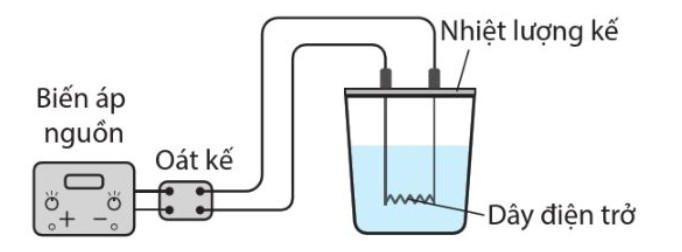
\includegraphics[scale=0.5]{figs/VN12-Y24-PH-SYL-004P-3}
}
\loigiai{
\begin{enumerate}[label=\alph*)]
	\item Đúng.
	\item Sai. Oát kế xác định công suất tiêu thụ điện của đoạn mạch.
	\item Đúng.
	\item Đúng.
\end{enumerate}
}
	\end{ex}

\begin{ex}
	Một chiếc thìa bằng đồng và một chiếc thìa bằng nhôm có cùng khối lượng và nhiệt độ ban đầu, được nhúng chìm vào cùng một cốc nước nóng (cao hơn nhiệt độ 2 thìa).
	\begin{enumerate}[label=\alph*)]
		\item 1 thìa toả nhiệt và 1 thìa thu nhiệt.
		\item Nhiệt độ cuối cùng của hai thìa bằng nhau.
		\item Khi có cân bằng nhiệt, nước bị giảm nhiệt độ.
		\item Nhiệt lượng của hai thìa trao đổi với nước là bằng nhau.
	\end{enumerate}
\loigiai{
\begin{enumerate}[label=\alph*)]
	\item Sai. Cả 2 thìa đều nhận nhiệt.
	\item Đúng.
	\item Đúng.
	\item Sai. Hai thìa có độ biến thiên nhiệt độ và khối lượng như nhau nhưng nhiệt dung riêng của chúng khác nhau nên nhiệt lượng trao đổi với nước của chúng khác nhau.
\end{enumerate}
}
	\end{ex}

\subsection{BÀI TẬP TỰ LUẬN}
\setcounter{ex}{0}
% ===================================================================
\begin{ex}
	\immini{
So sánh nhiệt dung riêng của thịt và của khoai tây, biết rằng khi cùng múc ra từ nồi canh hầm thì miếng thịt nguội nhanh hơn miếng khoai tây có cùng khối lượng.	

}{
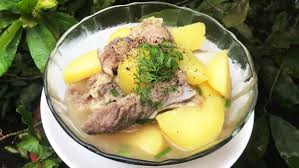
\includegraphics[scale=0.3]{figs/VN12-Y24-PH-SYL-004P-4}
}
\loigiai{
\begin{itemize}
	\item Nhiệt dung riêng là đại lượng thể hiện mức độ khó nóng, khó nguội của chất. Chất nào có nhiệt dung riêng lớn hơn thì khó nóng, khó nguội hơn.
	\item Khi cùng múc ra từ nồi canh hầm, miếng thịt nguội nhanh hơn miếng khoai tây cùng khối lượng. Điều này chứng tỏ thịt dễ nguội hơn khoai tây, nghĩa là nhiệt dung riêng của thịt nhỏ hơn nhiệt dung riêng của khoai tây.
\end{itemize}
}
	
	\end{ex}
% ===================================================================
\begin{ex}
Thùng nhôm khối lượng $\SI{1.2}{\kilogram}$ đựng $\SI{4}{\kilogram}$ nước ở $\SI{90}{\celsius}$. Cho biết nhiệt dung riêng của nhôm và nước lần lượt là $c_1=\SI{0.92}{\kilo\joule/\kilogram\cdot\kelvin}$, $c_2=\SI{4.186}{\kilo\joule/\left(\kilogram\cdot\kelvin\right)}$. Xác định nhiệt lượng thùng nước toả ra khi nhiệt độ giảm xuống còn $\SI{30}{\celsius}$.
	\loigiai{
	Nhiệt lượng do thùng nước toả ra:
	$$Q=\left(m_1c_1+m_2c_2\right)\Delta t=-\SI{1070880}{\joule}.$$
	Vậy nhiệt lượng do thùng nước toả ra là $\SI{1070880}{\joule}$.
	}
	
\end{ex}
% ===================================================================
\begin{ex}
	Để làm nguội nước nóng, người ta trộn $\SI{1.5}{\kilogram}$ nước ở $\SI{25}{\celsius}$ với $\SI{100}{\gram}$ nước ở $\SI{50}{\celsius}$. Xác định nhiệt độ cuối cùng của hỗn hợp khi cân bằng nhiệt.
	\loigiai{
	Khi có sự cân bằng nhiệt, tổng nhiệt lượng trao đổi trong hệ bằng 0:
	$$m_1c\left(t-t_1\right)+m_2c\left(t-t_2\right)=0$$
	$$\Leftrightarrow 1,5\left(t-\SI{25}{\celsius}\right)+0,1\left(t-\SI{50}{\celsius}\right)=0\Rightarrow t=\SI{26.5625}{\celsius}.$$
	}
	
\end{ex}
% ===================================================================
\begin{ex}
Muốn có nước ở nhiệt độ $t = \SI{50}{\celsius}$, người ta lấy $m_1 = \SI{3}{\kilogram}$ nước ở nhiệt độ $t_1 = \SI{100}{\celsius}$ trộn với nước ở nhiệt độ $t_2 =\SI{20}{\celsius}$. Hãy xác định khối lượng nước lạnh cần dùng.
	\loigiai{
		Khi cân bằng nhiệt, tổng nhiệt lượng trao đổi trong hệ bằng 0:
		$$m_1c\left(t_\text{cb}-t_1\right)+m_2c\left(t_\text{cb}-t_2\right)=0$$
		$$\Rightarrow m_2=\dfrac{m_1\left(t_1-t_\text{cb}\right)}{t_\text{cb}-t_2}=\SI{5}{\kilogram}.$$
	}
	
\end{ex}
% ===================================================================
\begin{ex}
Để xác định nhiệt dung riêng của một chất lỏng, người ta đổ chất lỏng đó vào $\SI{20}{\gram}$ nước ở nhiệt độ $\SI{100}{\celsius}$. Khi có cân bằng nhiệt, nhiệt độ của hỗn hợp đó là $\SI{37.5}{\celsius}$. Khối lượng hỗn hợp là $\SI{140}{\gram}$. Tính nhiệt dung riêng của chất lỏng đó, biết rằng nhiệt độ ban đầu của nó là $\SI{20}{\celsius}$ và hai chất lỏng không tác dụng hoá học với nhau. Cho nhiệt dung riêng của nước $c_2=\SI{4200}{\joule/\left(\kilogram\cdot\kelvin\right)}$.
	\loigiai{
	Gọi $m$ và $c$ lần lượt là khối lượng và nhiệt dung riêng của chất lỏng cần xác định nhiệt dung riêng.\\
	Khối lượng của chất lỏng đó:
	$$m=m_\text{hh}-m_\text{n}=\SI{120}{\gram}.$$
	Khi hệ đạt trạng thái cân bằng nhiệt thì tổng nhiệt lượng trao đổi của hệ bằng 0:
	$$mc\left(t_\text{cb}-t_0\right)+m_\text{n}c_\text{n}\left(t_\text{cb}-t_\text{0n}\right)=0$$
	$$\Rightarrow c=-\dfrac{m_\text{n}c_\text{n}\left(t_\text{cb}-t_\text{0n}\right)}{m\left(t_\text{cb}-t_0\right)}=\dfrac{\left(\SI{0.02}{\kilogram}\right)\cdot\left[\SI{4200}{\joule/\left(\kilogram\cdot\kelvin\right)}\right]\cdot\left(\SI{37.5}{\celsius}-\SI{100}{\celsius}\right)}{\left(\SI{0.12}{\kilogram}\right)\cdot\left(\SI{37.5}{\celsius}-\SI{20}{\celsius}\right)}=\SI{2500}{\joule/\left(\kilogram\cdot\kelvin\right)}.$$
	}
	
\end{ex}
% ===================================================================
\begin{ex}
	Để xác định nhiệt độ của một chiếc lò, người ta đốt nóng trong lò một cục sắt khối lượng $m_1=\SI{0.5}{\kilogram}$ rồi thả nhanh vào trong bình chứa $m_2=\SI{4}{\kilogram}$ nước có nhiệt độ ban đầu là $\SI{18}{\celsius}$. Nhiệt độ cuối cùng trong bình là $\SI{28}{\celsius}$. Hãy xác định nhiệt độ của lò. Bỏ qua trao đổi nhiệt với vỏ bình và quá trình nước hoá hơi khi tiếp xúc với cục sắt nóng. Cho nhiệt dung riêng của sắt là $c_1=\SI{460}{\joule/\left(\kilogram\cdot\kelvin\right)}$, nhiệt dung riêng của nước là $c_2=\SI{4200}{\joule/\left(\kilogram\cdot\kelvin\right)}$.
	\loigiai{
	Khi cân bằng nhiệt, tổng nhiệt lượng trao đổi trong hệ bằng 0:
	$$m_1c_1\left(t_\text{cb}-t_1\right)+m_2c_2\left(t_\text{cb}-t_2\right)=0\Rightarrow t_1\approx\SI{758.4}{\celsius}.$$
	}
	
\end{ex}
% ===================================================================
\begin{ex}
Trộn lẫn rượu vào nước, người ta thu được một hỗn hợp nặng $\SI{120.8}{\gram}$ ở nhiệt độ $\SI{30}{\celsius}$. Tính khối lượng nước và rượu đã pha, biết rằng ban đầu rượu ở nhiệt độ $\SI{10}{\celsius}$ và nước ở nhiệt độ $\SI{90}{\celsius}$. Cho nhiệt dung riêng của rượu và nước lần lượt là $\SI{2500}{\joule/\left(\kilogram\cdot\kelvin\right)}$, $\SI{4200}{\joule/\left(\kilogram\cdot\kelvin\right)}$.
	\loigiai{
		Gọi:
		\begin{itemize}
			\item $m_1, c_1, t_1$ lần lượt là khối lượng, nhiệt dung riêng và nhiệt độ ban đầu của rượu;
			\item $m_2, c_2, t_2$ lần lượt là khối lượng, nhiệt dung riêng và nhiệt độ ban đầu của nước.
		\end{itemize}
		Ta có:
		\begin{equation}
			\label{eq:4P-1}
			m_1+m_2=\SI{120.8}{\gram}=\SI{0.1208}{\kilogram}
		\end{equation}
		Khi hệ cân bằng nhiệt, tổng nhiệt lượng trao đổi trong hệ bằng 0:
		$$m_1c_1\left(t_\text{cb}-t_1\right)+m_2c_2\left(t_\text{cb}-t_2\right)=0$$
		\begin{equation}
			\label{eq:4P-2}
			50000m_1-252000m_2=0
		\end{equation}
		Từ (\ref{eq:4P-1}) và (\ref{eq:4P-2}) suy ra:
		\begin{equation*}
			\begin{cases}
				m_1=\SI{100.8}{\gram}\\
				m_2=\SI{20}{\gram}
			\end{cases}
			.
		\end{equation*}
	}
	
\end{ex}
% ===================================================================
\begin{ex}
	Bỏ một vật rắn khối lượng $\SI{100}{\gram}$ ở $\SI{100}{\celsius}$ vào $\SI{500}{\gram}$ nước ở $\SI{15}{\celsius}$ thì nhiệt độ sau cùng của vật là $\SI{16}{\celsius}$. Thay nước bằng $\SI{800}{\gram}$ chất lỏng khác ở $\SI{10}{\celsius}$ thì nhiệt độ sau cùng là $\SI{13}{\celsius}$. Tìm nhiệt dung riêng của vật rắn và chất lỏng. Cho nhiệt dung riêng của nước là $c = \SI{4200}{\joule/\left(\kilogram\cdot\kelvin\right)}$.
	\loigiai{
		\textbf{Khi bỏ vật rắn vào nước:}\\
		Khi cân bằng nhiệt, tổng nhiệt lượng trao đổi của vật rắn và nước bằng 0:
		$$m_vc_v\left(t_\text{cb}-t_v\right)+m_nc_n\left(t_\text{cb}-t_n\right)=0\Rightarrow c_v=\dfrac{m_nc_n\left(t_\text{cb}-t_n\right)}{m_v\left(t_v-t_\text{cb}\right)}=\SI{250}{\joule/\left(\kilogram\cdot\kelvin\right)}.$$
		\textbf{Khi bỏ vật rắn vào trong chất lỏng khác}\\
		Khi cân bằng nhiệt, tổng nhiệt lượng trao đổi của vật rắn và chất lỏng bằng 0:
		$$m_vc_v\left(t'_\text{cb}-t_v\right)+m_lc_l\left(t'_\text{cb}-t_l\right)\Rightarrow c_l=\dfrac{m_vc_v\left(t_v-t_\text{cb}\right)}{m_l\left(t'_\text{cb}-t_l\right)}=\SI{906.25}{\joule/\left(\kilogram\cdot\kelvin\right)}.$$
	}
	
\end{ex}
% ===================================================================
\begin{ex}
Người ta đổ $m_1 =\SI{200}{\gram}$ nước sôi có nhiệt độ $t_1 =\SI{100}{\celsius}$ vào một chiếc cốc có khối lượng $m_2 = \SI{120}{\gram}$ đang ở nhiệt độ $t_2 =\SI{20}{\celsius}$. sau khoảng thời gian $T = \SI{5}{\text{phút}}$, nhiệt độ của cốc nước bằng $t=\SI{40}{\celsius}$. Xem rằng sự mất nhiệt xảy ra một cách điều đặn, hãy xác định nhiệt lượng tỏa ra môi trường xung quanh trong mỗi giây. Cho nhiệt dung riêng nước và thuỷ tinh lần lượt là $c_1=\SI{4200}{\joule/\left(\kilogram\cdot\kelvin\right)}$, $c_2=\SI{840}{\joule/\left(\kilogram\cdot\kelvin\right)}$.
	\loigiai{Nhiệt lượng nước sôi toả ra để giảm nhiệt độ từ $\SI{100}{\celsius}$ còn $\SI{40}{\celsius}$:
		$$Q_\text{toả}=m_1c_1\left(t_1-t\right)=\SI{50400}{\joule}.$$
		Nhiệt lượng cốc thuỷ tinh thu vào để tăng nhiệt độ từ $\SI{20}{\celsius}$ lên $\SI{40}{\celsius}$:
		$$Q_\text{thu}=m_2c_2\left(t-t_2\right)=\SI{2016}{\joule}.$$
		Nhiệt lượng toả ra môi trường trong mỗi giây:
		$$w=\dfrac{Q_\text{toả}-Q_\text{thu}}{T}=\SI{161.28}{\joule/\second}.$$
	}
	
\end{ex}
% ===================================================================
\begin{ex}
	Trộn ba chất lỏng không tác dụng hoá học với nhau có khối lượng lần lượt là $m_1=\SI{2}{\kilogram}$, $m_2=\SI{3}{\kilogram}$, $m_3=\SI{4}{\kilogram}$. Biết nhiệt dung riêng và nhiệt độ ban đầu của mỗi chất lỏng lần lượt là $c_1=\SI{2000}{\joule/\left(\kilogram\cdot\kelvin\right)}$, $t_1=\SI{57}{\celsius}$, $c_2=\SI{4000}{\joule/\left(\kilogram\cdot\kelvin\right)}$, $t_2=\SI{63}{\celsius}$, $c_3=\SI{3000}{\joule/\left(\kilogram\cdot\kelvin\right)}$, $t_3=\SI{92}{\celsius}$. Nhiệt độ của hỗn hợp khi cân bằng nhiệt là bao nhiêu?
	\loigiai{Khi cân bằng nhiệt, tổng nhiệt lượng trao đổi trong hệ bằng 0:
		$$m_1c_1\left(t_\text{cb}-t_1\right)+m_2c_2\left(t_\text{cb}-t_2\right)+m_3c_3\left(t_\text{cb}-t_3\right)=0$$
		$$\Rightarrow t_\text{cb}=\dfrac{m_1c_1t_1+m_2c_2t_2+m_3c_3t_3}{m_1c_1+m_2c_2+m_3c_3}\approx\SI{74.6}{\celsius}.$$
	}
	
\end{ex}
% ===================================================================
\begin{ex}
	Một nhiệt lượng kế bằng nhôm có khối lượng $m_1 = \SI{100}{\gram}$ chứa $m_2 =\SI{400}{\gram}$ nước ở nhiệt độ $t_1 =\SI{10}{\celsius}$. Người ta thả vào nhiệt lượng kế một thỏi hợp kim nhôm và thiếc có khối lượng $m = \SI{200}{\gram}$ được nung nóng đến nhiệt độ $t_2 =\SI{120}{\celsius}$. Nhiệt độ cân bằng của hệ thống là $\SI{14}{\celsius}$. Tính khối lượng nhôm và thiếc có trong hợp kim. Cho nhiệt dung riêng của nhôm, nước, thiếc lần lượt là: $c_1 =\SI{900}{\joule/\left(\kilogram\cdot\kelvin\right)}$, $c_2=\SI{4200}{\joule/\left(\kilogram\cdot\kelvin\right)}$, $c_3 =\SI{230}{\joule/\left(\kilogram\cdot\kelvin\right)}$.
	\loigiai{Gọi $m_\text{nh}$, $m_\text{th}$ lần lượt là khối lượng của nhôm và thiếc trong hợp kim.\\
		Ta có:
		\begin{equation}
			\label{eq:4P-3}
			m_\text{nh}+m_\text{th}=\SI{0.2}{\kilogram}
		\end{equation}
		Khi hệ cân bằng nhiệt, tổng nhiệt lượng trao đổi trong hệ bằng 0:
		$$m_1c_1\left(t_\text{cb}-t_1\right)+m_2c_2\left(t_\text{cb}-t_1\right)+m_\text{nh}c_1\left(t_\text{cb}-t_2\right)+m_\text{th}c_3\left(t_\text{cb}-t_2\right)=0$$
		\begin{equation}
			\label{eq:4P-4}
			95400m_\text{nh}+24380m_\text{th}=7080
		\end{equation}
		Từ (\ref{eq:4P-3}) và (\ref{eq:4P-4}), suy ra:
		\begin{equation*}
			\begin{cases}
				m_\text{nh}\approx\SI{0.031}{\kilogram}\\
				m_\text{th}\approx\SI{0.169}{\kilogram}
			\end{cases}
		\end{equation*}
	}
	
\end{ex}
% ===================================================================
\begin{ex}
	Một khối sắt có khối lượng $m$ ở nhiệt độ $\SI{150}{\celsius}$ khi thả vào một bình nước thì làm nhiệt độ nước tăng từ $\SI{20}{\celsius}$ lên $\SI{60}{\celsius}$. Thả tiếp vào nước khối sắt thứ hai có khối lượng $\dfrac{m}{2}$ ở $\SI{100}{\celsius}$ thì nhiệt độ sau cùng của nước là bao nhiêu? Coi như chỉ có sự trao đổi nhiệt giữa khối sắt với nước và bỏ qua quá trình nước hoá thành hơi khi tiếp xúc với sắt nóng.
	\loigiai{	Gọi:
		\begin{itemize}
			\item $m_2$ là khối lượng nước trong bình;
			\item $c_1$, $c_2$ lần lượt là nhiệt dung riêng của sắt và nước;
			\item $t_1$, $t_2$ lần lượt là nhiệt độ ban đầu của thỏi sắt khối lượng $m$ và nước.
		\end{itemize}
		\textbf{Bỏ khối sắt khối lượng $m$ vào nước}\\
		Khi có cân bằng nhiệt, nhiệt lượng trao đổi trong hệ bằng 0:
		$$mc_1\left(t_\text{cb}-t_1\right)+m_2c_2\left(t_\text{cb}-t_2\right)=0\Rightarrow \dfrac{mc_1}{m_2c_2}=\dfrac{t_\text{cb}-t_2}{t_1-t_\text{cb}}=\dfrac{4}{9}.$$
		\textbf{Bỏ thêm khối sắt khối lượng $m/2$ vào nước}\\
		Khi có cân bằng nhiệt, nhiệt lượng trao đổi trong hệ bằng 0:
		$$\left(mc_1+m_2c_2\right)\left(t'_\text{cb}-t_\text{cb}\right)+\dfrac{m}{2}c_1\left(t'_\text{cb}-t'_1\right)=0$$
		$$\Rightarrow \Rightarrow t'_\text{cb}=\dfrac{mc_1\left(t_\text{cb}+\dfrac{t'_1}{2}\right)+m_2c_2t_\text{cb}}{1,5mc_1+m_2c_2}=\dfrac{\dfrac{4}{9}\cdot\left(\SI{60}{\celsius}+\SI{50}{\celsius}\right)+\SI{60}{\celsius}}{1,5\cdot\dfrac{4}{9}+1}\approx\SI{65.33}{\celsius}.$$
	}
	
\end{ex}
% ===================================================================
\begin{ex}
Có hai bình cách nhiệt. Bình 1 chứa $m_1 =\SI{2}{\kilogram}$ nước ở $t_1=\SI{20}{\celsius}$, bình 2 chứa $m_2 =\SI{4}{\kilogram}$ nước ở $t_2 =\SI{60}{\celsius}$. Người ta rót một lượng nước $m$ từ bình 1 sang bình 2, sau khi cân bằng nhiệt, người ta lại rót một lượng nước từ bình 2 sang bình 1. Nhiệt độ cân bằng ở bình 1 lúc này là $\SI{21.95}{\celsius}$.
\begin{enumerate}[label=\alph*)]
	\item Tính lượng nước $m$ rong mỗi lần rót và nhiệt độ cân bằng ở bình 2.
	\item Nếu tiếp tục thực hiện lần hai, tìm nhiệt độ cân bằng ở mỗi bình.
\end{enumerate}
	\loigiai{\begin{enumerate}[label=\alph*)]
			\item \begin{itemize}
				\item \textbf{Rót nước từ bình 1 sang bình 2}\\
				Khi cân bằng nhiệt, tổng nhiệt lượng trao đổi của $m$ và lượng nước ở bình 2 bằng 0:
				$$mc\left(t'_2-t_1\right)+m_2c\left(t'_2-t_2\right)=0$$
				\begin{equation}
					\label{eq:4P-5}
					m\left(t'_2-t_1\right)=m_2\left(t_2-t'_2\right)
				\end{equation}
				\item \textbf{Rót nước từ bình 2 sang bình 1}\\
				Khi cân bằng nhiệt, tổng nhiệt lượng trao đổi của $m$ và lượng nước ở bình 1 bằng 0:
				$$mc\left(t'_1-t\right)+\left(m_1-m\right)c\left(t'_1-t_1\right)=0$$
				\begin{equation}
					\label{eq:4P-6}
					m\left(t-t_1\right)=m_1\left(t'_1-t_1\right)
				\end{equation}
				Từ (\ref{eq:4P-5}) và (\ref{eq:4P-6}), suy ra:
				\begin{equation*}
					\begin{cases}
						t=\dfrac{m_2t_2-m_1\left(t'_1-t_1\right)}{m_2}\approx\SI{59}{\celsius}\\
						m=\dfrac{m_1m_2\left(t'_1-t_1\right)}{m_2\left(t_2-t_1\right)-m_1\left(t'_1-t_1\right)}\approx\SI{0.1}{\kilogram}
					\end{cases}
					.
				\end{equation*}
			\end{itemize}
			\item Thực hiện lần hai, nhiệt độ cân bằng của mỗi bình là
			$$t''_2=\dfrac{mt'_1+m_2t'_2}{m+m_2}=\SI{58.12}{\celsius};\quad t''_1=\dfrac{mt''_2+\left(m_1-m\right)t_1}{m_1}=\SI{23.76}{\celsius}.$$
		\end{enumerate}
	}
	
\end{ex}	
\newpage\section{NHIỆT NÓNG CHẢY RIÊNG - NHIỆT HOÁ HƠI RIÊNG}
\subsection{LÝ THUYẾT TRỌNG TÂM}
\subsubsection{Nhiệt nóng chảy riêng}
\begin{boxdl}
	Nhiệt nóng chảy riêng của một chất rắn có giá trị bằng nhiệt lượng cần cung cấp cho $\SI{1}{\kilogram}$ chất đó chuyển từ thể rắn sang thể lỏng tại nhiệt độ nóng chảy:
	\begin{equation}
		\lambda=\dfrac{Q}{m}
	\end{equation}
\end{boxdl}
với
\begin{itemize}
	\item $\lambda$: nhiệt nóng chảy riêng, đơn vị trong hệ SI là $\si{\joule/\kilogram}$;
	\item $Q$: nhiệt lượng khối chất rắn thu vào để nóng chảy hoàn toàn, đơn vị trong hệ SI là $\si{\joule}$;
	\item $m$: khối lượng của khối chất rắn, đơn vị trong hệ SI là $\si{\kilogram}$.
\end{itemize}
\subsubsection{Nhiệt hoá hơi riêng}
\begin{boxdl}
	Nhiệt hoá hơi riêng của một chất lỏng có giá trị bằng nhiệt lượng cần cung cấp cho $\SI{1}{\kilogram}$ chất lỏng đó hoá hơi hoàn toàn ở nhiệt độ sôi:
	\begin{equation}
		L=\dfrac{Q}{m}
	\end{equation}
\end{boxdl}
với
\begin{itemize}
	\item $L$: nhiệt hoá hơi riêng, đơn vị trong hệ SI là $\si{\joule/\kilogram}$;
	\item $Q$: nhiệt lượng khối chất lỏng thu vào để hoá hơi hoàn toàn, đơn vị trong hệ SI là $\si{\joule}$;
	\item $m$: khối lượng của khối chất lỏng, đơn vị trong hệ SI là $\si{\kilogram}$.
\end{itemize}
\subsection{VÍ DỤ MINH HOẠ}
\begin{dang}{Vận dụng biểu thức xác định nhiệt nóng chảy riêng}
\end{dang}
\begin{vd}
Một nhà máy thép mỗi lần luyện được 35 tấn thép. Cho nhiệt nóng chảy riêng của thép là $\SI{2.77E5}{\joule/\kilogram}$.
		\begin{enumerate}[label=\alph*)]
			\item Tính nhiệt lượng cần cung cấp để làm nóng chảy thép trong mỗi lần luyện của nhà máy ở nhiệt độ nóng chảy.
			\item Giả sử nhà máy sử dụng khí đốt để nấu chảy thép trong lò thổi (nồi nấu thép). Biết khi đốt cháy hoàn toàn $\SI{1}{\kilogram}$ khí đốt thì nhiệt lượng toả ra là $\SI{44E6}{\joule}$. Xác định khối lượng khí đốt cần sử dụng.
		\end{enumerate}

	\loigiai{
			\begin{enumerate}[label=\alph*)]
				\item Nhiệt lượng cần cung cấp để làm nóng chảy thép trong mỗi lần luyện của nhà máy ở nhiệt độ nóng chảy:
				$$Q=m\lambda=\left(\SI{35E3}{\kilogram}\right)\cdot\left(\SI{2.77E5}{\joule/\kilogram}\right)=\SI{96.95E8}{\joule}$$
				\item Khối lượng khí đốt cần sử dụng để nhiệt lượng toả ra như ở câu a):
				$$m=\dfrac{Q}{q}=\dfrac{\SI{96.95E8}{\joule}}{\SI{44E6}{\joule/\kilogram}}\approx\SI{220.34}{\kilogram}$$
		\end{enumerate}}
\end{vd}
	
	\begin{vd}
		Tính thời gian cần thiết để làm nóng chảy hoàn toàn $\SI{2}{\kilogram}$ đồng có nhiệt độ ban đầu $\SI{30}{\celsius}$, trong một lò nung điện có công suất $\SI{20000}{\watt}$. Biết chỉ có $\SI{50}{\percent}$ năng lượng tiêu thụ của lò được dùng vào việc làm đồng nóng lên và nóng chảy hoàn toàn ở nhiệt độ không đổi. Biết nhiệt độ nóng chảy của đồng là $\SI{1084}{\celsius}$. Cho nhiệt dung riêng, nhiệt nóng chảy riêng của đồng lần lượt là $\SI{380}{\joule/\left(\kilogram\cdot\kelvin\right)}$ và $\SI{1.8E5}{\joule/\kilogram}$.
	\loigiai{
				Nhiệt lượng khối đồng cần thu vào để tăng nhiệt độ từ $\SI{30}{\celsius}$ đến $\SI{1084}{\celsius}$:
				$$Q_1=mc\Delta t=\left(\SI{2}{\kilogram}\right)\cdot\left[\SI{380}{\joule/\left(\kilogram\cdot\kelvin\right)}\right]\cdot\left(\SI{1084}{\celsius}-\SI{30}{\celsius}\right)=\SI{801.04}{\kilo\joule}$$
				Nhiệt lượng khối đồng cần thu vào để nóng chảy hoàn toàn ở nhiệt độ $\SI{1084}{\celsius}$:
				$$Q_2=m\lambda=\left(\SI{2}{\kilogram}\right)\cdot\left(\SI{1.8E5}{\joule/\kilogram}\right)=\SI{360}{\kilo\joule}$$
				Tổng nhiệt lượng $\SI{2}{\kilogram}$ đồng cần thu vào để nóng chảy hoàn toàn từ nhiệt độ ban đầu $\SI{30}{\celsius}$:
				$$Q=Q_1+Q_2=\SI{1161.04}{\kilo\joule}$$
				Thời gian cần thiết để làm nóng chảy hoàn toàn khối đồng này:
				$$t=\dfrac{Q}{H\cdot\calP}=\dfrac{\SI{1161.04E3}{\joule}}{\left(\SI{50}{\percent}\right)\cdot\left(\SI{2E4}{\watt}\right)}\approx\SI{116}{\second}$$
			}
	\end{vd}
	
	\begin{dang}{Vận dụng biểu thức xác định nhiệt hoá hơi riêng}
			\end{dang}
\begin{vd}
Tính nhiệt lượng cần thiết để làm cho $\SI{1}{\kilogram}$ nước ở $\SI{25}{\celsius}$ chuyển thành hơi ở $\SI{100}{\celsius}$. Cho nhiệt dung riêng của nước là $\SI{4200}{\joule/\left(\kilogram\cdot\kelvin\right)}$, nhiệt hoá hơi riêng của nước ở $\SI{100}{\celsius}$ là $\SI{2.26E6}{\joule/\kilogram}$.
\loigiai{
		Nhiệt lượng nước thu vào để tăng nhiệt độ từ $\SI{25}{\celsius}$ đến $\SI{100}{\celsius}$:
		$$Q_1=mc\Delta t=\left(\SI{1}{\kilogram}\right)\cdot\left[\SI{4200}{\joule/\left(\kilogram\cdot\kelvin\right)}\right]\cdot\left(\SI{100}{\celsius}-\SI{25}{\celsius}\right)=\SI{315E3}{\joule}$$
		Nhiệt lượng nước cần thu vào để hoá thành hơi hoàn toàn ở $\SI{100}{\celsius}$:
		$$Q_2=mL=\left(\SI{1}{\kilogram}\right)\cdot\left(\SI{2.26E6}{\joule/\kilogram}\right)=\SI{226E4}{\joule}$$
		Tổng nhiệt lượng nước cần thu vào để hoá hơi hoàn toàn ở $\SI{100}{\celsius}$:
		$$Q=Q_1+Q_2=\SI{2.575}{\mega\joule}$$
	}

\end{vd}
		
		\begin{vd}
			Một ấm đun nước có công suất $\SI{500}{\watt}$ chứa $\SI{300}{\gram}$ nước ở nhiệt độ $\SI{20}{\celsius}$. Cho nhiệt dung riêng của nước là $\SI{4200}{\joule/\left(\kilogram\cdot\kelvin\right)}$, nhiệt hoá hơi riêng của nước ở $\SI{100}{\celsius}$ là $\SI{2.26E6}{\joule/\kilogram}$.
				\begin{enumerate}[label=\alph*)]
					\item Tính thời gian cần thiết để đun nước trong ấm để đạt đến nhiệt độ sôi.
					\item Sau khi nước đến nhiệt độ sôi, người ta để ấm tiếp tục đun nước sôi trong 2 phút. Tính khối lượng nước còn lại trong ấm và chỉ rõ điều kiện để thực hiện các tính toán đó.
				\end{enumerate}
			\loigiai{
					\begin{enumerate}[label=\alph*)]
						\item Nhiệt lượng nước trong ấm cần thu vào để tăng nhiệt độ từ $\SI{20}{\celsius}$ đến nhiệt độ sôi $\left(\SI{100}{\celsius}\right)$:
						$$Q_1=mc\Delta t=\left(\SI{0.3}{\kilogram}\right)\cdot\left[\SI{4200}{\joule/\left(\kilogram\cdot\kelvin\right)}\right]\cdot\left(\SI{100}{\celsius}-\SI{20}{\celsius}\right)=\SI{100800}{\joule}$$
						Thời gian đun sôi nước:
						$$t=\dfrac{Q_1}{\calP}=\dfrac{\SI{100800}{\joule}}{\SI{500}{\watt}}\approx\SI{201}{\second}$$
						\item Nhiệt lượng ấm toả ra trong 2 phút:
						$$Q_2=\calP\cdot t'=\left(\SI{500}{\watt}\right)\cdot\left(\SI{120}{\second}\right)=\SI{60}{\kilo\joule}$$
						Khối lượng nước bị hoá thành hơi ở nhiệt độ $\SI{100}{\celsius}$:
						$$m'=\dfrac{Q_2}{L}=\dfrac{\SI{60E3}{\joule}}{\SI{2.26E6}{\joule/\kilogram}}\approx\SI{26.55}{\gram}$$
						Khối lượng nước còn lại trong ấm:
						$$m_\text{nước}=m-m'=\SI{273.45}{\gram}$$
						Các tính toán trên được thực hiện với điều kiện:
						\begin{itemize}
							\item Nước được đun ở áp suất $\SI{1}{atm}$, do đó nhiệt độ sôi của nước là $\SI{100}{\celsius}$.
							\item Bỏ qua nhiệt lượng cung cấp cho vỏ ấm đun và toả ra môi trường.
							\item Bỏ qua sự bay hơi của nước trong quá trình đun.
						\end{itemize}
					\end{enumerate}
				}
		\end{vd}
	\begin{dang}
		{Áp dụng phương trình cân bằng nhiệt khi có sự chuyển thể}
		\begin{center}
			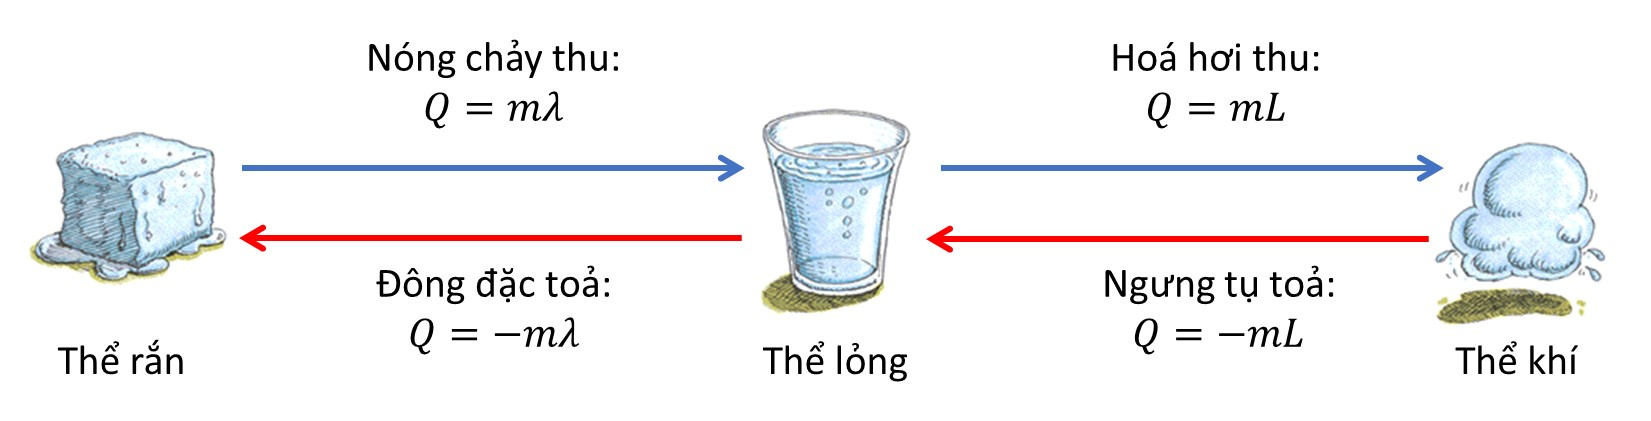
\includegraphics[width=0.8\linewidth]{figs/VN12-Y24-PH-SYL-006-1}
			\captionof{figure}{Sơ đồ chuyển thể}
		\end{center}
	\end{dang}
\begin{vd}
	Rót nước ở nhiệt độ $t_1=\SI{20}{\celsius}$ vào một nhiệt lượng kế. Thả vào trong nhiệt lượng kế một cục nước đá khối lượng $m_2=\SI{0.5}{\kilogram}$ và nhiệt độ $t_2=\SI{-15}{\celsius}$. Biết khối lượng nước đổ vào $m_1=m_2$. Cho biết nhiệt dung riêng của nước $c_1=\SI{4200}{\joule/\left(\kilogram\cdot\kelvin\right)}$, của nước đá $c_2=\SI{2100}{\joule/\left(\kilogram\cdot\kelvin\right)}$ và nhiệt nóng chảy riêng của nước đá $\lambda=\SI{3.4E5}{\joule/\kilogram}$. Bỏ qua sự trao đổi nhiệt với môi trường.
	\begin{enumerate}[label=\alph*)]
		\item Hãy cho biết cục nước đá có tan hết không?
		\item Nếu nước đá tan hết, hãy xác định nhiệt độ của hỗn hợp sau khi cân bằng nhiệt được thiết lập. Nếu nước đá không tan hết, hãy tính khối lượng nước đá đã tan.
	\end{enumerate}
\loigiai{
\begin{enumerate}[label=\alph*)]
	\item Nhiệt lượng nước $\SI{20}{\celsius}$ toả ra để giảm nhiệt độ xuống $\SI{0}{\celsius}$:
	$$Q_1=m_1c_1\left(0-t_1\right)=\left(\SI{0.5}{\kilogram}\right)\cdot\left[\SI{4200}{\joule/\left(\kilogram\cdot\kelvin\right)}\right]\cdot\left(\SI{0}{\celsius}-\SI{20}{\celsius}\right)=\SI{-42000}{\joule}$$
	Nhiệt lượng nước đá cần thu vào để tăng nhiệt độ từ $\SI{-15}{\celsius}$ đến $\SI{0}{\celsius}$ và nóng chảy hoàn toàn:
	$$Q_2=m_2c_2\left(0-t_2\right)+m_2\lambda$$
	$$\Leftrightarrow Q_2=\left(\SI{0.5}{\kilogram}\right)\cdot\left[\SI{2100}{\joule/\left(\kilogram\cdot\kelvin\right)}\right]\cdot\left(\SI{0}{\celsius}+\SI{15}{\celsius}\right)+\left(\SI{0.5}{\kilogram}\right)\cdot\left(\SI{3.4E5}{\joule/\kilogram}\right)=\SI{185750}{\joule}$$
	Vì $\left|Q_1\right|<Q_2$ nên nước đá chỉ tan được một phần.
	\item Vì nước đá chỉ tan một phần nên nhiệt độ của hỗn hợp khi cân bằng nhiệt là $\SI{0}{\celsius}$.\\
	Gọi $m'$ là khối lượng nước đá đã tan.\\
	Nhiệt lượng nước đá cần thu vào để tăng nhiệt độ từ $\SI{-15}{\celsius}$ đến $\SI{0}{\celsius}$ và nóng chảy một phần: $$Q_2'=m_2c_2\left(0-t_2\right)+m'\lambda$$
	Trạng thái cân bằng nhiệt được thiết lập khi tổng nhiệt lượng trao đổi trong hệ bằng 0:
	$$Q_1+Q_2'=0$$
	$$\Leftrightarrow Q_1+m_2c_2\left(0-t_2\right)+m'\lambda=0$$
	\begin{eqnarray*}
		\Rightarrow m'&=&-\dfrac{Q_1+m_2c_2\left(0-t_2\right)}{\lambda}\\
		\Leftrightarrow m'&=&-\dfrac{\SI{-42000}{\joule}+\left(\SI{0.5}{\kilogram}\right)\cdot\left[\SI{2100}{\joule/\left(\kilogram\cdot\kelvin\right)}\right]\cdot\left(\SI{0}{\celsius}+\SI{15}{\celsius}\right)}{\SI{3.4E5}{\joule/\kilogram}}\\
		\Rightarrow m'&\approx&\SI{77.2}{\gram}.
	\end{eqnarray*}
	Vậy khối lượng nước đá đã tan là $\SI{77.2}{\gram}$.
	
	
\end{enumerate}
}
\end{vd}
% ========================================================================
\begin{vd}
	Dẫn $m_1=\SI{100}{\gram}$ hơi nước ở $t_1=\SI{100}{\celsius}$ vào một bình cách nhiệt đựng nước đá ở $t_2=\SI{-4}{\celsius}$. Nước đá bị tan hoàn toàn và nhiệt độ nước trong bình sau khi cân bằng nhiệt là $\SI{10}{\celsius}$. Tìm khối lượng nước đá trong bình. Biết nhiệt nóng chảy riêng của nước đá là $\lambda=\SI{3.4E5}{\joule/\kilogram}$, nhiệt hoá hơi riêng của nước ở $\SI{100}{\celsius}$ là $L=\SI{2.3E6}{\joule/\kilogram}$, nhiệt dung riêng của nước là $c_1=\SI{4200}{\joule/\left(\kilogram\cdot\kelvin\right)}$, nhiệt dung riêng của nước đá là $c_2=\SI{2100}{\joule/\left(\kilogram\cdot\kelvin\right)}$. Bỏ qua sự trao đổi nhiệt với môi trường.
	\loigiai{
	Gọi $\xsi{m}{\left(\kilogram\right)}$ là khối lượng nước đá trong bình.\\
	Nhiệt lượng hơi nước toả ra để ngưng tụ hoàn toàn ở $\SI{100}{\celsius}$ và giảm nhiệt độ từ $\SI{100}{\celsius}$ xuống $\SI{10}{\celsius}$:
	$$Q_1=-m_1L+m_1c_1\left(t_\text{cb}-t_1\right)$$
	$$\Leftrightarrow Q_1=-\left(\SI{0.1}{\kilogram}\right)\cdot\left(\SI{2.3E6}{\joule/\kilogram}\right)+\left(\SI{0.1}{\kilogram}\right)\cdot\left[\SI{4200}{\joule/\left(\kilogram\cdot\kelvin\right)}\right]\cdot\left(\SI{10}{\celsius}-\SI{100}{\celsius}\right)=\SI{-267800}{\joule}$$
	Nhiệt lượng nước đá thu vào để tăng nhiệt độ từ $\SI{-4}{\celsius}$ lên $\SI{0}{\celsius}$, nóng chảy hoàn toàn ở $\SI{0}{\celsius}$ rồi tăng nhiệt độ lên $\SI{10}{\celsius}$:
	$$Q_2=mc_2\left(0-t_2\right)+m\lambda+mc_1\left(t_\text{cb}-0\right)$$
	$$\Leftrightarrow Q_2=m\cdot\left[\SI{2100}{\joule/\left(\kilogram\cdot\kelvin\right)}\right]\cdot\left(\SI{0}{\celsius}+\SI{4}{\celsius}\right)+m\cdot\left(\SI{3.4E5}{\joule/\kilogram}\right)+m\cdot\left[\SI{4200}{\joule/\left(\joule\cdot\kelvin\right)}\right]\cdot\left(\SI{10}{\celsius}-\SI{0}{\celsius}\right)=390400m$$
	Hệ đạt trạng thái cân bằng nhiệt khi tổng nhiệt lượng trao đổi trong hệ bằng 0:
	\begin{eqnarray*}
		&&Q_1+Q_2=0\\
		&\Leftrightarrow& -267800+390400m=0\\
		&\Rightarrow& m\approx\SI{0.686}{\kilogram}.
	\end{eqnarray*}
}
\end{vd}
\subsection{BÀI TẬP TRẮC NGHIỆM}
\setcounter{ex}{0}
\Opensolutionfile{ans}[ans/G12Y24B6TN]		
% ===================================================================
\begin{ex}
Khi vật rắn tinh thể đang nóng chảy thì đại lượng nào của vật sau đây là không thay đổi?	
\choice
{Thể tích}
{Nội năng}
{\True Nhiệt độ}
{Hình dạng}
\loigiai{}
\end{ex}
% ===================================================================
\begin{ex}
	Điều nào sau đây là \textbf{đúng} khi nói về nhiệt nóng chảy riêng?
	\choice
	{Nhiệt nóng chảy riêng của chất rắn là nhiệt lượng cần cung cấp cho vật rắn trong quá trình nóng chảy}
	{Các chất có khối lượng bằng nhau thì có nhiệt độ nóng chảy như nhau}
	{Nhiệt nóng chảy riêng của chất rắn tỉ lệ thuận với khối lượng của vật}
	{\True Đơn vị của nhiệt nóng chảy riêng là $\si{\joule/\kilogram}$}
	\loigiai{}
\end{ex}
% ===================================================================
\begin{ex}
Điều nào sau đây là \textbf{đúng} khi nói về nhiệt nóng chảy riêng của chất rắn?
	\choice
	{Nhiệt nóng chảy riêng của một chất rắn có độ lớn bằng nhiệt lượng cần cung cấp để làm nóng chảy $\SI{1}{\kilogram}$ chất đó ở nhiệt độ nóng chảy}
	{Đơn vị của nhiệt nóng chảy riêng là joule trên kilogram $\left(\si{\joule/\kilogram}\right)$}
	{Các chất khác nhau thì nhiệt nóng chảy riêng của chúng khác nhau}
	{\True Cả A, B, C đều đúng}
	\loigiai{}
\end{ex}
% ===================================================================
\begin{ex}
	Nhiệt nóng chảy riêng của đồng là $\SI{1.8E5}{\joule/\kilogram}$. Câu nào dưới đây là \textbf{đúng}?
	\choice
	{Khối đồng sẽ toả ra nhiệt lượng $\SI{1.8E5}{\joule}$ khi nóng chảy hoàn toàn}
	{\True Mỗi kilogram đồng cần thu nhiệt lượng $\SI{1.8E5}{\joule}$ để hoá lỏng hoàn toàn ở nhiệt độ nóng chảy}
	{Khối đồng cần nhu nhiệt lượng $\SI{1.8E5}{\joule}$ để hoá lỏng}
	{Mỗi kilogram đồng toả ra nhiệt lượng $\SI{1.8E5}{\joule}$ khi hoá lỏng hoàn toàn}
	\loigiai{}
\end{ex}
% ===================================================================
\begin{ex}
	Đơn vị của nhiệt hoá hơi riêng của chất lỏng là
	\choice
	{\True $\si{\joule/\kilogram}$}
	{$\si{\joule\cdot\kilogram}$}
	{$\si{\kilogram/\joule}$}
	{$\si{\joule}$}
	\loigiai{}
\end{ex}
% ===================================================================
\begin{ex}
	Nhiệt hoá hơi riêng của nước là $\SI{2.3E6}{\joule/\kilogram}$. Câu nào dưới đây là \textbf{đúng nhất}?
	\choice
	{Mỗi lượng nước bất kì cần thu một lượng nhiệt $\SI{2.3E6}{\joule}$ để bay hơi hoàn toàn}
	{Mỗi kilogram nước cần thu một lượng nhiệt là $\SI{2.3E6}{\joule}$ để bay hơi hoàn toàn}
	{Mỗi kilogram nước sẽ toả ra một lượng nhiệt là $\SI{2.3E6}{\joule}$ khi bay hơi hoàn toàn ở nhiệt độ sôi}
	{\True Mỗi kilogram nước cần thu một lượng nhiệt là $\SI{2.3E6}{\joule}$ để bay hơi hoàn toàn ở nhiệt độ sôi và áp suất chuẩn}
	\loigiai{}
\end{ex}
% ===================================================================
\begin{ex}
	Biết nhiệt nóng chảy riêng của nước đá là $\SI{3.34E5}{\joule/\kilogram}$. Nhiệt lượng cần cung cấp để làm nóng chảy $\SI{500}{\gram}$ nước đá ở $\SI{0}{\celsius}$ là
	\choice
	{$\SI{7E7}{\joule}$}
	{$\SI{167}{\joule}$}
	{\True $\SI{167}{\kilo\joule}$}
	{$\SI{167e6}{\joule}$}
	\loigiai{	$$Q=m\lambda=\left(\SI{0.5}{\kilogram}\right)\cdot\left(\SI{3.34E5}{\joule/\kilogram}\right)=\SI{167}{\kilo\joule}$$}
\end{ex}
% ===================================================================
\begin{ex}
	Biết nhiệt nóng chảy riêng của nước đá là $\SI{3.34E5}{\joule/\kilogram}$. Người ta cung cấp nhiệt lượng $\SI{5.01E5}{\joule}$ thì có thể làm nóng chảy hoàn toàn bao nhiêu kilogram nước đá?
	\choice
	{$\SI{16.7}{\kilogram}$}
	{\True $\SI{1.5}{\kilogram}$}
	{$\SI{8.35}{\kilogram}$}
	{$\SI{0.668}{\kilogram}$}
	\loigiai{$$m=\dfrac{Q}{\lambda}=\SI{1.5}{\kilogram}$$}
\end{ex}
% ===================================================================
\begin{ex}
	Biết nhiệt dung riêng của nước là $c=\SI{4190}{\joule/\left(\kilogram\cdot\kelvin\right)}$ và nhiệt hoá hơi riêng của nước là $L=\SI{2.26E6}{\joule/\kilogram}$. Để làm cho $\SI{200}{\gram}$ nước ở $\SI{10}{\celsius}$ sôi ở $\SI{100}{\celsius}$ và $\SI{10}{\percent}$ lượng nước này hoá hơi khi sôi thì cần cung cấp một nhiệt lượng \textbf{gần nhất} là
	\choice
	{$\SI{169}{\kilo\joule}$}
	{\True $\SI{121}{\kilo\joule}$}
	{$\SI{189}{\kilo\joule}$}
	{$\SI{212}{\kilo\joule}$}
	\loigiai{	Nhiệt lượng cần cung cấp:
		$$Q=mc\left(100-t\right)+\SI{10}{\percent}mL\approx\SI{121}{\kilo\joule}$$}
\end{ex}
% ===================================================================
\begin{ex}
Cho biết nhiệt dung riêng của nước $\SI{4180}{\joule/\left(\kilogram\cdot\kelvin\right)}$ và nhiệt hoá hơi riêng của nước là $\SI{2.3E6}{\joule/\kilogram}$. Nhiệt lượng cần cung cấp cho $\SI{10}{\kilogram}$ nước ở $\SI{25}{\celsius}$ chuyển thành hơi ở $\SI{100}{\celsius}$ là
	\choice
	{$\SI{18450}{\kilo\joule}$}
	{\True $\SI{26135}{\kilo\joule}$}
	{$\SI{84500}{\kilo\joule}$}
	{$\SI{804500}{\kilo\joule}$}
	\loigiai{	$$Q=mc\Delta t+mL=\SI{26135}{\kilo\joule}$$}
\end{ex}
% ===================================================================
\begin{ex}
	Nước có nhiệt dung riêng $c=\SI{4180}{\joule/\left(\kilogram\cdot\kelvin\right)}$ và nhiệt hoá hơi riêng $L=\SI{2.3E6}{\joule/\kilogram}$. Nhiệt lượng toả ra khi $\SI{4}{\kilogram}$ hơi nước ở $\SI{100}{\celsius}$ ngưng tụ thành nước ở $\SI{22}{\celsius}$ là 
	\choice
	{$\SI{11504160}{\joule}$}
	{$\SI{12504160}{\joule}$}
	{\True $\SI{10504160}{\joule}$}
	{$\SI{13504160}{\joule}$}
	\loigiai{Nhiệt lượng toả ra khi $\SI{4}{\kilogram}$ hơi nước ở $\SI{100}{\celsius}$ ngưng tụ thành nước ở $\SI{22}{\celsius}$ là 
		$$Q=mL+mc\left(t_0-t\right)=\SI{10504160}{\joule}$$}
\end{ex}
% ===================================================================
\begin{ex}
	Người ta có $\SI{5}{\kilogram}$ nước đá ở $\SI{-10}{\celsius}$, cho biết nhiệt dung riêng của nước đá là $\SI{1090}{\joule/\kilogram}$ và nhiệt nóng chảy riêng của nước đá là $\SI{3.4E5}{\joule/\kilogram}$. Nhiệt lượng cần cung cấp để khối đá trên tan hoàn toàn thành nước ở $\SI{0}{\celsius}$ là
	\choice
	{$\SI{4.45}{\kilo\joule}$}
	{\True $\SI{1.8}{\mega\joule}$}
	{$\SI{1.9}{\mega\joule}$}
	{$\SI{1.7}{\mega\joule}$}
	\loigiai{Nhiệt lượng cần cung cấp để khối đá trên tan hoàn toàn thành nước ở $\SI{0}{\celsius}$ là
		$$Q=m\lambda+mc\left(0-t_0\right)=\SI{1804500}{\joule}$$
	}
\end{ex}

% ===================================================================
\begin{ex}
Để xác định nhiệt hóa hơi riêng của nước, người ta làm thí nghiệm sau: đưa $\SI{10}{\gram}$ hơi nước ở nhiệt độ $\SI{100}{\celsius}$ vào một nhiệt lượng kế chứa $\SI{290}{\gram}$ nước ở $\SI{20}{\celsius}$. Nhiệt độ cuối của hệ là $\SI{40}{\celsius}$. Cho biết nhiệt dung của nhiệt lượng kế là  $\SI{46}{\joule/\kelvin}$, nhiệt dung riêng của nước là $\SI{4.18}{\joule/\left(\gram\cdot\kelvin\right)}$. Nhiệt hoá hơi riêng của nước là 
	\choice
	{$\SI{6900}{\joule/\gram}$}
	{\True $\SI{2265.6}{\joule/\gram}$}
	{$\SI{4600}{\joule/\gram}$}
	{$\SI{3200}{\joule/\gram}$}
	\loigiai{Khi hệ cân bằng nhiệt, tổng nhiệt lượng trao đổi trong hệ bằng 0:
		$$-m_\text{hơi}L+m_\text{hơi}c\left(t_\text{cb}-t_\text{hơi}\right)+m_\text{nước}c\left(t_\text{cb}-t_\text{n}\right)=0\Rightarrow L=\SI{2265.6}{\joule/\gram}$$}
\end{ex}
% ===================================================================
\begin{ex}
	Đổ $\SI{100}{\gram}$ nước ở $\SI{40}{\celsius}$ vào một khối nước đá lớn ở $\SI{0}{\celsius}$. Cho nhiệt nóng chảy riêng của nước đá là $\lambda=\SI{80}{cal/\gram\cdot\kelvin}$ và nhiệt dung riêng của nước đá là $c=\SI{1}{cal/\gram\cdot\kelvin}$. Khối lượng nước đá tan chảy là
	\choice
	{$\SI{200}{\gram}$}
	{\True $\SI{50}{\gram}$}
	{$\SI{25}{\gram}$}
	{$\SI{100}{\gram}$}
	\loigiai{	Khối lượng nước đá tan:
		$$m=\dfrac{m_nc_n\Delta t}{\lambda}=\SI{50}{\gram}$$}
\end{ex}
% ===================================================================
\begin{ex}
\immini{Một chậu đựng hỗn hợp nước và nước đá có khối lượng $\SI{10}{\kilogram}$. Chậu để trong phòng và người ta theo dõi nhiệt độ của hỗn hợp. Đồ thị biểu thị sự phụ thuộc nhiệt độ theo thời gian cho ở hình bên. Cho nhiệt dung riêng của nước là $c=\SI{4200}{\joule/\left(\kilogram\cdot\kelvin\right)}$ và nhiệt nóng chảy riêng của nước đá là $\lambda=\SI{3.4E5}{\joule/\kilogram}$. Bỏ qua sự trao đổi nhiệt với chậu. Khối lượng nước đá trong hỗn hợp ban đầu là
	\choice
	{$\SI{0.296}{\kilogram}$}
	{$\SI{1.48}{\kilogram}$}
	{$\SI{0.21}{\kilogram}$}
	{\True $\SI{1.235}{\kilogram}$}
	\loigiai{	$$\dfrac{m_\text{đ}\lambda}{m_\text{hh}c\Delta t}=5\Rightarrow m_\text{đ}\approx\SI{1.235}{\kilogram}$$}}
{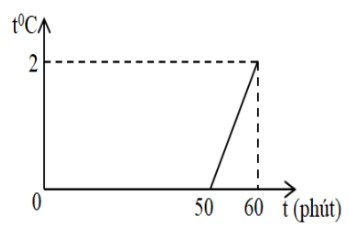
\includegraphics[scale=0.7]{figs/VN12-Y24-PH-SYL-005P-1}

}
\end{ex}
% ===================================================================
\begin{ex}
Người ta thả một cục nước đá khối lượng $\SI{80}{\gram}$ ở $\SI{0}{\celsius}$ vào một cốc nhôm đựng $\SI{0.4}{\kilogram}$ nước ở $\SI{20}{\celsius}$ đặt trong nhiệt lượng kế. Biết khối lượng cốc nhôm là $\SI{0.2}{\kilogram}$. Cho nhiệt nóng chảy riêng của nước đá là $\SI{3.4E5}{\joule/\kilogram}$, nhiệt dung riêng của nhôm là $\SI{880}{\joule/\left(\kilogram\cdot\kelvin\right)}$ và của nước là $\SI{4180}{\joule/\left(\kilogram\cdot\kelvin\right)}$. Bỏ qua sự mất mát nhiệt do truyền ra ngoài. Nhiệt độ của nước khi nước đá đã tan hết là
	\choice
	{\True $\SI{4.5}{\celsius}$}
	{$\SI{5.5}{\celsius}$}
	{$\SI{6.5}{\celsius}$}
	{$\SI{7.5}{\celsius}$}
	\loigiai{		Khi cân bằng nhiệt, tổng nhiệt lượng trao đổi trong hệ bằng 0:
		$$m_\text{đ}\lambda+m_\text{đ}c\left(t_\text{cb}-0\right)+m_\text{n}c\left(t_\text{cb}-t_\text{n}\right)=0\Rightarrow t_\text{cb}\approx\SI{4.47}{\celsius}$$}
\end{ex}
% ===================================================================
\begin{ex}
	Lấy $\SI{0.01}{\kilogram}$ hơi nước ở $\SI{100}{\celsius}$ cho ngưng tụ trong bình nhiệt lượng kế chứa $\SI{0.2}{\kilogram}$ nước ở $\SI{9.5}{\celsius}$; nhiệt độ cuối cùng của nước là $\SI{40}{\celsius}$. Cho nhiệt dung riêng của nước là $c=\SI{4180}{\joule/\left(\kilogram\cdot\kelvin\right)}$. Nhiệt hoá hơi riêng của nước là
	\choice
	{$\SI{3.1e6}{\joule/\kilogram}$}
	{$\SI{2.8e6}{\joule/\kilogram}$}
	{\True $\SI{2.3e6}{\joule/\kilogram}$}
	{$\SI{1.4e6}{\joule/\kilogram}$}
	\loigiai{Áp dụng phương trình cân bằng nhiệt:
		$$m_1L+m_1c\left(100-t_\text{cb}\right)=m_2c\left(t_\text{cb}-t_2\right)$$
		$$\Leftrightarrow 0,01L+0,01\cdot4180\cdot\left(100-40\right)=0,2\cdot4180\cdot\left(40-9,5\right)\Rightarrow L=\SI{2.299E6}{\joule/\kilogram}$$
	}
\end{ex}
% ===================================================================
\begin{ex}
	Một khối nước đá có khối lượng $\SI{0.2}{\kilogram}$ ở $\SI{-20}{\celsius}$. Cho biết nhiệt dung riêng của nước đá là $\SI{2.09E3}{\joule/\left(\kilogram\cdot\kelvin\right)}$, nhiệt nóng chảy riêng của nước đá là $\SI{3.4E5}{\joule/\kilogram}$, nhiệt dung riêng của nước là $\SI{4.18E3}{\joule/\left(\kilogram\cdot\kelvin\right)}$, nhiệt hoá hơi riêng của nước là $\SI{2.3E6}{\joule/\kilogram}$. Nhiệt lượng cần cung cấp cho khối nước đá để nó hoá hơi hoàn toàn ở $\SI{100}{\celsius}$ là
	\choice
	{$Q=\SI{205.96}{\kilo\joule}$}
	{\True $Q=\SI{619.96}{\kilo\joule}$}
	{$Q=\SI{159.96}{\kilo\joule}$}
	{$Q=\SI{460}{\kilo\joule}$}
	\loigiai{Nhiệt lượng cần cung cấp cho khối nước đá để nó hoá hơi hoàn toàn ở $\SI{100}{\celsius}$ là
		$$Q=mc_\text{đ}\left(0-t_\text{đ}\right)+m\lambda+mc\left(t_s-0\right)+mL=\SI{619.96}{\kilo\joule}$$}
\end{ex}
% ===================================================================
\begin{ex}
	Cần cung cấp một nhiệt lượng bằng bao nhiêu để làm cho $m=\SI{200}{\gram}$ nước lấy ở $t_1=\SI{10}{\celsius}$ sôi ở $t_2=\SI{100}{\celsius}$ và $\SI{10}{\percent}$ khối lượng của nó đã hoá hơi khi sôi. Biết nhiệt dung riêng của nước là $c=\SI{4190}{\joule/\left(\kilogram\cdot\kelvin\right)}$ và nhiệt hoá hơi riêng của nước là $L=\SI{2.26E6}{\joule/\kilogram}$. Chọn đáp án \textbf{đúng}.
	\choice
	{$\SI{129525}{\joule}$}
	{$\SI{110610}{\joule}$}
	{\True $\SI{120620}{\joule}$}
	{$\SI{130610}{\joule}$}
	\loigiai{$$Q=mc\Delta t+\SI{10}{\percent}mL=\SI{120620}{\joule}$$}
\end{ex}
% ===================================================================
\begin{ex}
	Lấy $\SI{0.01}{\kilogram}$ cho ngưng tụ trong bình nhiệt lượng kế chứa $\SI{0.2}{\kilogram}$ nước ở $\SI{9.5}{\celsius}$. Nhiệt độ cuối cùng đo được là $\SI{40}{\celsius}$. Cho nhiệt dung riêng của nước là $c=\SI{4180}{\joule/\left(\kilogram\cdot\kelvin\right)}$. Nhiệt hoá hơi riêng của nước là
	\choice
	{$\SI{6.9E6}{\joule/\kilogram}$}
	{\True $\SI{2.3E6}{\joule/\kilogram}$}
	{$\SI{4.6E6}{\joule/\kilogram}$}
	{$\SI{3.2E6}{\joule/\kilogram}$}
	\loigiai{Khi hệ cân bằng nhiệt, tổng nhiệt lượng trao đổi trong hệ bằng 0:
		$$-m_\text{hơi}L+m_\text{hơi}c\left(t_\text{cb}-t_\text{hơi}\right)+m_\text{nước}c\left(t_\text{cb}-t_\text{nước}\right)=0\Rightarrow L\approx\SI{2.3E6}{\joule/\kilogram}$$
	}
\end{ex}
% ===================================================================
\begin{ex}
	Để xác định nhiệt nóng chảy riêng của thiếc, người ta đổ $\SI{350}{\gram}$ thiếc nóng chảy ở nhiệt độ $\SI{232}{\celsius}$ vào $\SI{330}{\gram}$ nước ở $\SI{7}{\celsius}$ đựng trong một nhiệt lượng kế có nhiệt dung bằng $\SI{100}{\joule/\kelvin}$. Sau khi cân bằng nhiệt, nhiệt độ của nước trong nhiệt lượng kế là $\SI{32}{\celsius}$. Biết nhiệt dung riêng của nước và thiếc rắn lần lượt là $\SI{4.2}{\joule/\left(\gram\cdot\kelvin\right)}$, $\SI{0.23}{\joule/\left(\gram\cdot\kelvin\right)}$. Nhiệt nóng chảy riêng của thiếc \textbf{gần với giá trị nào nhất} sau đây?
	\choice
	{\True $\SI{60}{\joule/\gram}$}
	{$\SI{73}{\joule/\gram}$}
	{$\SI{89}{\joule/\gram}$}
	{$\SI{96}{\joule/\gram}$}
	\loigiai{Khi hệ cân bằng nhiệt, tổng nhiệt lượng trao đổi trong hệ bằng 0:
		$$-m_\text{th}\lambda+m_\text{th}c_\text{th}\left(t_\text{cb}-t_\text{th}\right)+\left(m_\text{n}c_\text{n}+c_\text{nlk}\right)\cdot\left(t_\text{cb}-t_\text{n}\right)=0$$
		$$\Rightarrow \lambda=\dfrac{m_\text{th}c_\text{th}\left(t_\text{cb}-t_\text{th}\right)+\left(m_\text{n}c_\text{n}+c_\text{nlk}\right)\cdot\left(t_\text{cb}-t_\text{n}\right)}{m_\text{th}}\approx\SI{60.1}{\joule/\gram}$$
	}
\end{ex}

% ===================================================================
\begin{ex}
Một viên đạn chì phải có tốc độ tối thiểu bằng bao nhiêu để khi nó va chạm vào vật cứng thì nóng chảy hoàn toàn? Cho rằng, $\SI{80}{\percent}$ động năng của viên đạn chuyển thành nội năng của nó khi va chạm; nhiệt độ của viên đạn trước khi va chạm là $\SI{127}{\celsius}$. Cho biết nhiệt dung riêng của chì là $\SI{130}{\joule/\left(\kilogram\cdot\kelvin\right)}$; nhiệt độ nóng chảy của chì là $\SI{327}{\celsius}$ và nhiệt nóng chảy riêng của chì là $\lambda=\SI{25}{\kilo\joule/\kilogram}$.
	\choice
	{\True $\SI{357}{\meter/\second}$}
	{$\SI{324}{\meter/\second}$}
	{$\SI{352}{\meter/\second}$}
	{$\SI{457}{\meter/\second}$}
	\loigiai{	Nhiệt lượng cần thiết để viên đạn tăng nhiệt độ từ $\SI{127}{\celsius}$ lên $\SI{327}{\celsius}$ và nóng chảy hoàn toàn:
		$$Q=mc\left(t-t_0\right)+m\lambda=51000m$$
		Áp dụng định lý động năng:
		$$0-\dfrac{1}{2}mv^2_0=-\dfrac{Q}{0.8}$$
		$$\Leftrightarrow \dfrac{1}{2}mv^2_0=\dfrac{51000m}{0.8}\Rightarrow v_0\approx\SI{357}{\meter/\second}$$}
\end{ex}
% ===================================================================
\begin{ex}
	Trong một nhiệt lượng kế bằng nhôm khối lượng $m_\text{nl}=\SI{300}{\gram}$ có một cục nước đá nặng $m_\text{nđ}\left(\si{\gram}\right)$. Nhiệt độ của nhiệt lượng kế và nước đá là $t_1=\SI{-5}{\celsius}$. Sau đó người ta cho $m_\text{hn}\left(\si{\gram}\right)$ hơi nước ở $t_2=\SI{100}{\celsius}$ vào nhiệt lượng kế và khi đã cân bằng nhiệt độ thì nhiệt độ của nhiệt lượng kế là $t_3=\SI{25}{\celsius}$. Lúc đó, trong nhiệt lượng kế có $\SI{500}{\gram}$ nước. Cho biết nhiệt hoá hơi riêng của nước là $L=\SI{2.26E3}{\joule/\gram}$, nhiệt nóng chảy của nước đá $\lambda=\SI{334}{\joule/\gram}$, nhiệt dung riêng của nhôm, của nước đá và của nước lần lượt là $c_\text{nl}=\SI{0.88}{\joule/\gram\cdot\kelvin}$, $c_\text{nđ}=\SI{2.09}{\joule/\gram\cdot\kelvin}$ và $c_\text{n}=\SI{4.19}{\joule/\gram\cdot\kelvin}$. Giá trị của $\left(m_\text{nđ}-3m_\text{hn}\right)$ \textbf{gần với giá trị nào nhất} sau đây?
	\choice
	{$\SI{226}{\gram}$}
	{$\SI{253}{\gram}$}
	{$\SI{269}{\gram}$}
	{\True $\SI{192}{\gram}$}
	\loigiai{Ta có:
		\begin{equation}
			\label{eq:6P-1}
			m_\text{nđ}+m_\text{hn}=\SI{500}{\gram}
		\end{equation}
		Khi có cân bằng nhiệt, tổng nhiệt lượng trao đổi trong hệ bằng 0:
		$$-m_\text{hn}L+m_\text{hn}c\left(t_3-t_2\right)+m_\text{nđ}c_\text{nđ}\left(0-t_1\right)+m_\text{nđ}\lambda+m_\text{nl}c_\text{nl}\left(t_3-t_1\right)+m_\text{nđ}c_\text{n}\left(t_3-0\right)=0$$
		\begin{equation}
			\label{eq:6P-2}
			-2574.25m_\text{hn}+449,2m_\text{nđ}=-7920
		\end{equation}
		Từ (\ref{eq:6P-1}) và (\ref{eq:6P-2}), suy ra:
		$$\begin{cases}
			m_\text{hn}=\SI{76.9}{\gram}\\
			m_\text{nđ}=\SI{423.1}{\gram}
		\end{cases}$$
		Như vậy, $\left(m_\text{nđ}-3m_\text{hn}\right)=\SI{192.4}{\gram}$
	}
\end{ex}
\Closesolutionfile{ans}
	\subsection{TRẮC NGHIỆM ĐÚNG/SAI}
	\setcounter{ex}{0}
% =======================================================================
\begin{ex}
		Bảng dưới đây là nhiệt độ nóng chảy của một số chất.
	\begin{center}
		\begin{tabular}{|C{5cm}|C{1.25cm}|C{1.25cm}|C{1.25cm}|C{1.25cm}|C{1.25cm}|C{1.25cm}|C{1.25cm}|}
			\hline
			\thead{Chất} & Nhôm & Nước đá & Rượu & Sắt & Đồng & Thuỷ ngân & Muối ăn\\
			\hline
			\thead{Nhiệt độ nóng chảy\\ $\left(\si{\celsius}\right)$}& 660 & 0 & -117 & 1535 & 1083 & -39 & 801\\
			\hline
		\end{tabular}
	\end{center}
	\begin{enumerate}[label=\alph*)]
		\item Chất có nhiệt độ nóng chảy cao nhất là đồng.
		\item Chất có nhiệt độ nóng chảy thấp nhất là thuỷ ngân.
		\item Có thể dùng nhiệt kế rượu để đo nhiệt độ thấp tới $\SI{-50}{\celsius}$.
		\item Có thể dùng nhiệt kế thuỷ ngân để đo nhiệt độ thấp tới $\SI{-50}{\celsius}$.
	\end{enumerate}
	\loigiai{	\begin{enumerate}[label=\alph*)]
			\item Sai.
			\item Sai. Chất có nhiệt độ nóng chảy thấp nhất là rượu.
			\item Đúng.
			\item Sai. Thuỷ ngân đã đông đặc ở $\SI{-39}{\celsius}$.
	\end{enumerate}}
	\end{ex}
% =======================================================================
\begin{ex}
	\immini{
		Nếu đặt tô kem lỏng vào giữa chậu nước đá, kem sẽ chỉ lạnh đi nhưng rất khó có thể đông đặc lại. Tuy nhiên, nếu em cho thêm một ít muối vào chậu nước đá này thì kem lỏng có thể đông đặc lại thành đá như hình minh hoạ bên dưới rất nhanh.
		\begin{enumerate}[label=\alph*)]
			\item Kem lạnh đi do nhận nhiệt từ nước đá.
			\item Khi cân bằng nhiệt diễn ra, nếu trong đá có lẫn nước thì nhiệt độ của hỗn hợp nước và nước đá là $\SI{0}{\celsius}$.
			\item Nước muối thấm qua tô vào kem và làm tăng nhiệt độ đông đặc của kem (kem đông đặc ở nhiệt độ trên $\SI{0}{\celsius}$).
			\item Nhiệt độ đông đặc của nước trong thau sau khi cho muối vào bị giảm.
		\end{enumerate}
}{
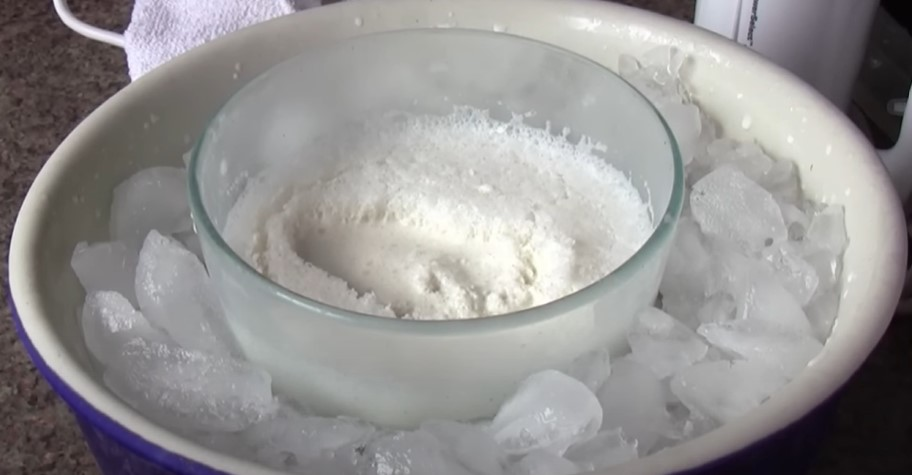
\includegraphics[scale=0.3]{figs/VN12-Y24-PH-SYL-006P-1}
%\caption{Kem lỏng nhanh chóng đông thành đá khi cho muối vào thau nước đá}
}
\loigiai{\begin{enumerate}[label=\alph*)]
		\item Sai. Kem lạnh đi là do kem toả nhiệt cho thau đá.
		\item Đúng.
		\item Sai. Nước muối không thể thấm qua tô do sự liên kết của các phân tử chất rắn rất chặt chẽ. Ở điều kiện tiêu chuẩn, nhiệt độ đông đặc của nước là $\SI{0}{\celsius}$.
		\item Đúng. Nhiệt độ đông đặc của nước trong thau sau khi cho muối vào bị giảm là do sự phân li của các ion trong phân tử muối ăn làm ảnh hưởng đến liên kết hydrogen của các phân tử nước. Do đó, các phân tử nước khó liên kết lại với nhau thành thể rắn hơn
\end{enumerate}}
	\end{ex}
\subsection{BÀI TẬP TỰ LUẬN}
\setcounter{ex}{0}
% ========================================================================
\begin{ex}

	Trên hình vẽ dưới đây biểu diễn đồ thị nhiệt độ của một chất theo thời gian trong quá trình đông đặc. Dựa vào đồ thị, em hãy trả lời các câu hỏi sau:
	\begin{center}
		\begin{tikzpicture}  
			\begin{axis}[  ultra thick,
				xmin=0,  
				xmax=28,  
				xtick={0,5,...,25},
				ytick={-40,-30,...,30},
				minor x tick num=1,
				minor y tick num=4,
				ymin=-48,  
				ymax=35, 
				samples=300,
				axis lines=center, 
				grid style={step=1, line width =0.4pt, color=gray!30!white},
				grid=both,
				major grid style={line width=0.8pt,gray!60!white},
				xlabel=$\xsi{t}{\left(\si{\text{phút}}\right)}$, 		ylabel=$\xsi{t}{\celsius}$,
				every axis y label/.style={at=(current axis.above origin),anchor=south},  
				every axis x label/.style={at=(current axis.right of origin),anchor=west},  ]
				\draw [ultra thick, red] (axis cs: 0,12) --(axis cs: 7.5,-40)--(axis cs: 25,-40)--(axis cs: 25.72,-45); 
				\filldraw[black] (axis cs:0,12) circle (1pt) node[right] {A};
				\filldraw[black] (axis cs:7.5,-40) circle (1pt) node[below] {B}; 
				\filldraw[black] (axis cs:25,-40) circle (1pt) node[below left] {C}; 
			\end{axis}
			\node[left] at (-0.1,3.2) {0};  
		\end{tikzpicture}
	\end{center}
	\begin{enumerate}[label=\alph*)]
		\item Các đoạn AB và BC biểu diễn quá trình gì?
		\item Nhiệt độ ban đầu của chất này là bao nhiêu?
		\item Nhiệt độ đông đặc của chất này là bao nhiêu?
		\item Quá trình làm nguội và đông đặc diễn ra bao lâu?
	\end{enumerate}

\loigiai{
	\begin{enumerate}[label=\alph*)]
		\item AB là quá trình chất này giảm nhiệt độ (quá trình làm nguội), BC là quá trình chất này đông đặc.
		\item Nhiệt độ ban đầu của chất này là $\SI{12}{\celsius}$.
		\item Nhiệt độ đông đặc của chất này là $\SI{-40}{\celsius}$.
		\item Qúa trình làm nguội diễn ra trong $\SI{7.5}{\text{phút}}$, quá trình đông đặc diễn ra trong $\SI{17.5}{\text{phút}}$.
	\end{enumerate}}
	\end{ex}
% ========================================================================
\begin{ex}
	Vận động viên chạy Marathon mất rất nhiều nước trong khi thi đấu. Các vận động viên thường chỉ có thể chuyển hoá khoảng $\SI{20}{\percent}$ năng lượng hoá học dự trữ trong cơ thể thành năng lượng dùng cho các hoạt động của cơ thể, đặc biệt là hoạt động chạy. Phần năng lượng còn lại chuyển thành nhiệt thải ra ngoài nhờ sự bay hơi của nước qua hô hấp và da để giữ nhiệt độ cơ thể ổn định. Nếu vận động viên dùng hết $\SI{11000}{\kilo\joule}$ trong cuộc thi thì có khoảng bao nhiêu lít nước đã thoát ra khỏi cơ thể? Coi nhiệt độ cơ thể của vận động viên hoàn toàn không đổi và nhiệt hoá hơi riêng của nước trong cơ thể vận động viên là $\SI{2.45E6}{\joule/\kilogram}$.
	\loigiai{
		Lượng hơi nước thoát ra khỏi cơ thể vận động viên:
		$$m=\dfrac{\SI{80}{\percent}\cdot W}{L}\approx\SI{3.59}{\kilogram}$$
	}
	\end{ex}
% ========================================================================
\begin{ex}
	Để hàn các linh kiện bị đứt trong mạch điện tử, người thợ sửa chữa thường sử dụng mỏ hàn điện để làm nóng chảy dây thiếc hàn. Biết rằng loại thiếc hàn sử dụng là hỗn hợp của thiếc và chì với tỉ lệ khối lượng $63:37$, khối lượng một cuộn dây thiếc hàn là $\SI{50}{\gram}$. Biết thiếc và chì có nhiệt nóng chảy riêng lần lượt là $\SI{0.61E5}{\joule/\kilogram}$ và $\SI{0.25E5}{\joule/\kilogram}$. Nhiệt lượng mỏ hàn cần cung cấp để làm nóng chảy hết một cuộn dây thiếc hàn ở nhiệt độ nóng chảy bằng bao nhiêu?
	\loigiai{
		$$\dfrac{m_t}{m_c}=\dfrac{63}{37}\xrightarrow{m_t+m_c=\SI{50}{\gram}}\begin{cases}
			m_t=\SI{31.5}{\gram}\\
			m_c=\SI{18.5}{\gram}
		\end{cases}$$
		Nhiệt lượng mỏ hàn cần cung cấp để làm nóng chảy hết một cuộn dây thiếc hàn ở nhiệt độ nóng chảy:
		$$Q=m_t\lambda_t+m_c\lambda_c=\SI{2384}{\joule}$$
	}
\end{ex}
% ========================================================================
\begin{ex}
Một ấm đun nước có công suất $\SI{500}{\watt}$ chứa $\SI{300}{\gram}$ nước. Cho nhiệt hoá hơi riêng của nước là $\SI{2E6}{\joule/\kilogram}$. Sau khi đun nước trong ấm đến nhiệt độ sôi, người ta để ấm tiếp tục đun nước sôi trong 2 phút. Bỏ qua sự mất mát nhiệt. Khối lượng nước còn lại trong ấm bằng bao nhiêu?
\loigiai{
	Lượng nước hoá hơi:
	$$m'=\dfrac{\calP t}{L}=\SI{0.03}{\kilogram}=\SI{30}{\gram}$$
	Lượng nước còn lại trong ấm là
	$$m=M-m'=\SI{270}{\gram}$$
}
\end{ex}
% ========================================================================
\begin{ex}
		Người ta bỏ một cục nước đá khối lượng $m_1=\SI{100}{\gram}$ vào một nhiệt lượng kế bằng đồng có khối lượng $m_2=\SI{125}{\gram}$, thì nhiệt độ của nhiệt lượng kế và nước đá là $t_1=\SI{-20}{\celsius}$. Tính nhiệt lượng cần thiết để làm tan được một nửa lượng nước đá trên. Cho nhiệt dung riêng của đồng là $c_2=\SI{380}{\joule/\kilogram\cdot\kelvin}$, của nước đá là $c_1=\SI{2100}{\joule/\kilogram\cdot\kelvin}$, nhiệt nóng chảy riêng của nước đá là $\SI{3.34E5}{\joule/\kilogram}$.
	\loigiai{
	Nhiệt lượng cần cung cấp cho nhiệt lượng kế để nước đá tan được 1 nửa:
	$$Q=\left(m_1c_1+m_2c_2\right)\cdot\left(0-t_1\right)+\dfrac{m_1}{2}\lambda=\SI{21850}{\joule}.$$	
	}
\end{ex}
% ========================================================================
\begin{ex}
Người ta trộn $m_1=\SI{500}{\gram}$ nước đá với $m_2=\SI{500}{\gram}$ nước ở cùng nhiệt độ $t_1=\SI{0}{\celsius}$ vào một xô nước ở nhiệt độ $\SI{50}{\celsius}$. Khối lượng tổng cộng của chúng là $m=\SI{2}{\kilogram}$. Tính nhiệt độ của xô nước khi có cân bằng nhiệt. Cho nhiệt dung riêng của nước $c=\SI{4200}{\joule/\left(\kilogram\cdot\kelvin\right)}$, nhiệt nóng chảy riêng của nước đá $\lambda=\SI{3.4E5}{\joule/\kilogram}$. Bỏ qua khối lượng và sự thu nhiệt của xô.
\loigiai{
	Khi cân bằng nhiệt, tổng nhiệt lượng trao đổi trong hệ bằng 0:
	$$m_1\lambda+\left(m_1+m_2\right)c\left(t_\text{cb}-0\right)+\left(m-m_1-m_2\right)c\left(t_\text{cb}-t_0\right)=0$$
	$$\Leftrightarrow 0,5\cdot\SI{3.4E5}{}+1\cdot4200\cdot t_\text{cb}+1\cdot4200\left(t_\text{cb}-50\right)=0\Rightarrow t_\text{cb}\approx\SI{4.76}{\celsius}$$
}
\end{ex}
% ========================================================================
\begin{ex}
Bỏ $\SI{20}{\gram}$ tuyết có lẫn nước ở $\SI{0}{\celsius}$ vào nhiệt lượng kế chứa $\SI{250}{\gram}$ nước ở $\SI{15}{\celsius}$. Khi cân bằng nhiệt, nhiệt độ của nhiệt lượng kế giảm $\SI{5}{\celsius}$. Hỏi khối lượng nước lẫn trong tuyết là bao nhiêu? Biết nhiệt nóng chảy riêng của nước đá là $\lambda=\SI{3.4E5}{\joule/\kilogram}$, nhiệt dung riêng của nước $c=\SI{4200}{\joule/\left(\kilogram\cdot\kelvin\right)}$. Bỏ qua nhiệt dung của nhiệt lượng kế.
\loigiai{
	Gọi $m_1$, $m_2$ lần lượt là khối lượng của nước và đá trong tuyết.\\
	Ta có:
	\begin{equation*}
		m_1+m_2=\SI{0.02}{\kilogram}
	\end{equation*}
	Khi cân bằng nhiệt, tổng nhiệt lượng trao đổi trong hệ bằng 0:
	$$m_2\lambda+\left(m_1+m_2\right)c\left(t_\text{cb}-0\right)+m_\text{n}c\left(t_\text{cb}-t_\text{n}\right)=0$$
	$$\Rightarrow m_2\approx\SI{0.013}{\kilogram}=\SI{13}{\gram}$$
	Như vậy, khối lượng nước lẫn trong tuyết là $m_1\approx\SI{7}{\gram}$
}
\end{ex}
% ========================================================================
\begin{ex}
Trong ruột cục nước đá lớn ở $\SI{0}{\celsius}$ có một cái hốc với thể tích bằng $V=\SI{160}{\centi\meter^3}$. Người ta rót vào hốc đó $\SI{60}{\gram}$ ở nhiệt độ $\SI{75}{\celsius}$. Cho khối lượng riêng của nước $D_1=\SI{1}{\gram/\centi\meter^3}$ và của nước đá $D_2=\SI{0.9}{\gram/\centi\meter^3}$, nhiệt dung riêng của nước là $c=\SI{4200}{\joule/\left(\kilogram\cdot\kelvin\right)}$ và để làm nóng chảy hoàn toàn $\SI{1}{\kilogram}$ nước đá ở nhiệt độ nóng chảy cần cung cấp cho khối nước đá này một nhiệt lượng $\SI{3.36E5}{\joule}$. Hỏi khi nước nguội hẳnn thì thể tích hốc rỗng còn lại là bao nhiêu $\si{\centi\meter^3}$?
\loigiai{
	Nhiệt lượng do nước toả ra để giảm nhiệt độ từ $\SI{75}{\celsius}$ về $\SI{0}{\celsius}$:
	$$Q_\text{toả}=m_\text{n}c\left(0-t_\text{n}\right)=\SI{18900}{\joule}$$
	Thể tích nước rót vào hốc:
	$$V_n=\dfrac{m_n}{D_1}=\SI{60}{\centi\meter^3}$$
	Khối lượng nước đá tan:
	$$m_\text{đá}=\dfrac{Q_\text{thu}}{\lambda}=\dfrac{Q_\text{toả}}{\lambda}=\SI{56.25}{\gram}$$
	Thể tích nước đá bị tan là
	$$V_\text{đ}=\dfrac{m_\text{đ}}{D_2}=\SI{62.5}{\centi\meter^3}$$
	Thể tích nước tạo thành do đá tan:
	$$V_1=\dfrac{m_\text{đ}}{D_1}=\SI{56.25}{\centi\meter^3}$$
	Thể tích phần rỗng còn lại:
	$$V+V_\text{đ}-V_1-V_\text{n}=\SI{106.25}{\centi\meter^3}$$
}
\end{ex}
% ========================================================================
\begin{ex}
Dẫn hơi nước ở $\SI{100}{\celsius}$ vào một bình nước đang có nhiệt độ $\SI{20}{\celsius}$ dưới áp suất bình thường.
\begin{enumerate}[label=\alph*)]
	\item Khối lượng nước trong bình tăng lên bao nhiêu lần khi nhiệt độ của nó đạt tới $\SI{100}{\celsius}$.
	\item Khi nhiệt độ của nước đạt tới $\SI{100}{\celsius}$, nếu tiếp tục dẫn hơi nước ở $\SI{100}{\celsius}$ vào bình thì có thể làm cho nước trong bình có thể sôi được không?
\end{enumerate}
Cho:
\begin{itemize}
	\item nhiệt dung riêng của nước $c=\SI{4200}{\joule/\left(\kilogram\cdot\kelvin\right)}$;
	\item nhiệt hoá hơi riêng của nước $L=\SI{2.3E6}{\joule/\kilogram}$.
\end{itemize}
	\loigiai{
	\begin{enumerate}[label=\alph*)]
		\item Gọi $m$ là khối lượng hơi nước ngưng tụ và $M$ là khối lượng nước có sẵn trong bình.\\
		Khi có cân bằng nhiệt, tổng nhiệt lượng trao đổi trong hệ bằng 0:
		$$-mL+Mc\left(100-t_0\right)=0\Rightarrow m=0,146M.$$
		$$\Rightarrow \dfrac{m+M}{M}=1,146.$$
		\item Nước không thể sôi vì hệ đã đạt trạng thái cân bằng nhiệt ở $\SI{100}{\celsius}$ nên không thể nhận thêm nhiệt lượng để hoá thành hơi.
	\end{enumerate}
	}
\end{ex}
% ========================================================================
\begin{ex}
	Người ta dẫn hơi nước ở $\SI{100}{\celsius}$ vào một nhiệt lượng kế chứa $\SI{100}{\gram}$ nước đá ở $\SI{0}{\celsius}$. Sau khi nước đá tan hết, khối lượng nước trong nhiệt lượng kế là bao nhiêu? Cho nhiệt nóng chảy riêng của nước đá là $\lambda=\SI{3.4E5}{\joule/\kilogram}$; nhiệt hoá hơi riêng của nước $L=\SI{2.26E6}{\joule/\kilogram}$; nhiệt dung riêng của nước $c=\SI{4200}{\joule/\left(\kilogram\cdot\kelvin\right)}$ và bỏ qua nhiệt dung của nhiệt lượng kế.
	\loigiai{
		Gọi $m$ là khối lượng hơi nước ngưng tụ thành nước và $m_\text{đ}$ là khối lượng nước đá nóng chảy.\\
		Khi có cân bằng nhiệt, tổng nhiệt lượng trao đổi của hệ bằng 0:
		$$m_\text{đ}\lambda-mL+mc\left(0-100\right)=0\Rightarrow m=\SI{0.0127}{\kilogram}.$$
		Lượng nước tăng thêm trong bình:
		$$m_\text{n}=m_\text{đ}+m=\SI{112.7}{\gram}.$$
	}
\end{ex}
% ========================================================================
\begin{ex}
		Người ta đổ $\xsi{m_1}{\left(\kilogram\right)}$ nước ở nhiệt độ $t_1=\SI{60}{\celsius}$ vào $\xsi{m_2}{\left(\kilogram\right)}$ nước đá ở nhiệt độ $t_2=\SI{-5}{\celsius}$. Khi có cân bằng nhiệt, lượng nước thu được là $m=\SI{50}{\kilogram}$ có nhiệt độ $t=\SI{25}{\celsius}$. Xác định $m_1$ và $m_2$. Cho nhiệt dung riêng của nước và nước đá lần lượt là $c_1=\SI{4200}{\joule/\left(\kilogram\cdot\kelvin\right)}$, $c_2=\SI{2100}{\kilogram/\left(\kilogram\cdot\kelvin\right)}$, nhiệt nóng chảy riêng của nước đá $\lambda=\SI{3.4E5}{\joule/\kilogram}$.
	\loigiai{
	Ta có:
	\begin{equation}
		\label{eq:6P-1}
		m_1+m_2=\SI{50}{\kilogram}
	\end{equation}	
	Khi cân bằng nhiệt xảy ra, tổng nhiệt lượng trao đổi trong hệ bằng 0:
	$$m_1c_1\left(t_\text{cb}-t_1\right)+m_2c_2\left(0-t_2\right)+m_2\lambda+m_2c_1\left(t_\text{cb}-t_1\right)=0.$$
	\begin{equation}
		\label{eq:6P-2}
		-147000m_1+455500m_2=0
	\end{equation}
	Từ (\ref{eq:6P-1}) và (\ref{eq:6P-2}), suy ra:
	\begin{equation*}
		\begin{cases}
			m_1=\SI{37.8}{\kilogram}\\
			m_2=\SI{12.2}{\kilogram}
		\end{cases}
	\end{equation*}
	}
\end{ex}
% ========================================================================
\begin{ex}
Cho $\SI{100}{\gram}$ nước đá ở nhiệt độ $t_1=\SI{0}{\celsius}$ vào $\SI{300}{\gram}$ nước ở nhiệt độ $t_2=\SI{20}{\celsius}$. Hỏi nước đá có tan hết không? Nếu không, em hãy tính khối lượng nước đá còn lại.\\
Cho nhiệt nóng chảy riêng của nước đá là $\lambda=\SI{3.4E5}{\joule/\kilogram}$ và nhiệt dung riêng của nước là $c=\SI{4200}{\joule/\left(\kilogram\cdot\kelvin\right)}$.
	\loigiai{
	Nhiệt lượng nước đá thu vào để nóng chảy hoàn toàn
	$$Q_\text{thu}=m_\text{đ}\lambda=\SI{3.4E4}{\joule}.$$
	Nhiệt lượng nước toả ra để giảm nhiệt độ từ $\SI{20}{\celsius}$ xuống $\SI{0}{\celsius}$:
	$$Q_\text{toả}=m_\text{n}c\left(t_\text{n}-0\right)=\SI{2.52E4}{\joule}.$$
	Vì $Q_\text{thu}>Q_\text{toả}$ nên nước đá không tan hết.\\
	Gọi $m$ là khối lượng nước đá tan.\\
	Do nước đá không tan hết nên nhiệt độ của hệ khi cân bằng nhiệt là $\SI{0}{\celsius}$.\\
	Khối lượng nước đá tan:
	$$m=\dfrac{Q_\text{toả}}{\lambda}\approx\SI{0.07412}{\kilogram}\approx\SI{74.12}{\gram}.$$
	Vậy: khối lượng nước đá còn lại là xấp xỉ $\SI{25.88}{\gram}$.
	}
\end{ex}
% ========================================================================
\begin{ex}
\begin{enumerate}[label=\alph*)]
	\item Tính nhiệt lượng do $\SI{500}{\gram}$ nước ở $\SI{30}{\celsius}$ toả ra khi nhiệt độ của nó hạ xuống $\SI{0}{\celsius}$.
	\item Để biến lượng nước trên thành nước đá, người ta bỏ vào nước trên một khối nước đá ở nhiệt độ $\SI{-10}{\celsius}$. Tính khối lượng nước đá tối thiểu cần dùng.
\end{enumerate}
Cho:
\begin{itemize}
	\item nhiệt dung riêng của nước $c_\text{n}=\SI{4200}{\joule/\left(\kilogram\cdot\kelvin\right)}$;
	\item nhiệt dung riêng của nước đá $c_\text{đ}=\SI{2000}{\joule/\left(\kilogram\cdot\kelvin\right)}$;
	\item nhiệt nóng chảy riêng của nước đá $\lambda=\SI{3.4E5}{\joule/\kilogram}$.
\end{itemize}
	\loigiai{
		\begin{enumerate}[label=\alph*)]
			\item Nhiệt lượng do $\SI{500}{\gram}$ nước đá toả ra để hạ nhiệt độ từ $\SI{30}{\celsius}$ xuống $\SI{0}{\celsius}$:
			$$Q_1=m_\text{n}c_\text{n}\left(t_\text{n}-0\right)=\SI{63}{\kilo\joule}.$$
			\item Nhiệt lượng tối thiểu lượng nước trên cần toả ra để đông thành đá (nước đá ở $\SI{0}{\celsius}$):
			$$Q_\text{toả}=Q_1+m_\text{n}\lambda=\SI{233}{\kilo\joule}.$$
			Nhiệt lượng do đá ở $\SI{-10}{\celsius}$ thu vào để tăng nhiệt độ lên $\SI{0}{\celsius}$ bằng nhiệt lượng do nước toả ra, do đó khối lượng đá cần dùng:
			$$m_\text{đá}=\dfrac{Q_\text{toả}}{c_\text{đ}\left(0-t_\text{đ}\right)}=\SI{11.65}{\kilogram}.$$
		\end{enumerate}
	}
\end{ex}
% ========================================================================
\begin{ex}
Cho đồ thị biểu diễn sự thay đổi nhiệt độ của khối chất lỏng theo nhiệt lượng cung cấp có dạng như hình bên. Biết nhiệt dung riêng của chất lỏng đó là $c=\SI{2500}{\joule/\left(\kilogram\cdot\kelvin\right)}$. Xác định nhiệt hoá hơi riêng của chất lỏng trên.
\begin{center}
	\begin{tikzpicture}  
		\begin{axis}[  ultra thick,
			xmin=0,  
			xmax=14,  
			xtick={1.8,12.6},
			ytick={20,80},
			minor x tick num=0,
			minor y tick num=0,
			ymin=0,  
			ymax=90, 
			samples=300,
			axis lines=center, 
			xlabel=$\xsi{Q}{\left(\xsi{10^5}{\joule}\right)}$, 		ylabel=$\xsi{t}{\celsius}$,
			every axis y label/.style={at=(current axis.above origin),anchor=south},  
			every axis x label/.style={at=(current axis.right of origin),anchor=west},  ]
			\draw [line width=1.0pt,dashed,gray!60!white] (axis cs: 0,80) --(axis cs: 1.8,80)--(axis cs: 1.8,0);
			\draw [line width=1.0pt,dashed,gray!60!white] (axis cs: 12.6,80)--(axis cs: 12.6,0);
			\draw [ultra thick, red] (axis cs: 0,20) --(axis cs: 1.8,80)--(axis cs: 12.6,80)--(axis cs: 13.8,84); 
			
		\end{axis}
		\node[left] at (-0.1,3.2) {0};  
	\end{tikzpicture}
	
\end{center}
	\loigiai{
		Nhiệt lượng chất lỏng thu vào để tăng nhiệt độ từ $\SI{20}{\celsius}$ lên $\SI{80}{\celsius}$:
		$$Q_1=mc\left(t_2-t_1\right).$$
		Nhiệt lượng chất lỏng thu vào để hoá hơi hoàn toàn ở nhiệt độ sôi:
		$$Q_2-Q_1=mL.$$
		Ta có:
		$$\dfrac{Q_2-Q_1}{Q_1}=\dfrac{L}{c\Delta t}\Rightarrow L=\left(\dfrac{Q_2-Q_1}{Q_1}\right)c\Delta t=\left(\dfrac{\SI{12.6}{\joule}-\SI{1.8}{\joule}}{\SI{1.8}{\joule}}\right)\cdot\left[\SI{2500}{\joule/\left(\kilogram\cdot\kelvin\right)}\right]\cdot\left(\SI{80}{\celsius}-\SI{20}{\celsius}\right)=\SI{9E5}{\joule/\kilogram}.$$
	}
\end{ex}
% ========================================================================
\begin{ex}
Thả 1 quả cầu bằng thép có khối lượng $m_1=\SI{2}{\kilogram}$ được nung tới nhiệt độ $\SI{600}{\celsius}$ vào một hỗn hợp nước và đá ở $\SI{0}{\celsius}$. Hỗn hợp có khối lượng tổng cộng là $m_2=\SI{2}{\kilogram}$.
\begin{enumerate}[label=\alph*)]
	\item Tính khối lượng nước đá có trong hỗn hợp. Biết nhiệt độ cuối cùng của hỗn hợp là $\SI{50}{\celsius}$.
	\item Thực ra, trong quá trình trên có một lớp nước tiếp xúc trực tiếp với quả cầu bị hoá thành hơi nên nhiệt độ cuối cùng của hỗn hợp chỉ là $\SI{48}{\celsius}$. Tính khối lượng nước đã hoá thành hơi.
\end{enumerate}
Cho:
\begin{itemize}
	\item nhiệt dung riêng của thép $c_1=\SI{460}{\joule/\left(\kilogram\cdot\kelvin\right)}$;
	\item nhiệt dung riêng của nước $c_2=\SI{4200}{\joule/\left(\kilogram\cdot\kelvin\right)}$;
	\item nhiệt nóng chảy riêng của nước đá $\lambda=\SI{3.4E5}{\joule/\kilogram}$;
	\item nhiệt hoá hơi riêng của nước $L=\SI{2.3E6}{\joule/\kilogram}$.
\end{itemize}
	\loigiai{
	\begin{enumerate}[label=\alph*)]
		\item Gọi $m_\text{n}$ và $m_\text{đ}$ lần lượt là khối lượng nước và đá có trong hỗn hợp ban đầu.\\
		Khi cân bằng nhiệt, tổng nhiệt lượng trao đổi trong hệ bằng 0:
		$$m_\text{đ}\lambda+m_2c_2\left(t_\text{cb}-0\right)+m_1c_1\left(t_\text{cb}-t_1\right)=0$$
		$$\Leftrightarrow m_\text{đ}=\dfrac{m_1c_1\left(t_1-t_\text{cb}\right)-m_2c_2t_\text{cb}}{\lambda}=\SI{0.253}{\kilogram}.$$
		\item Phần nhiệt lượng bị mất mát đi khi chỉ đạt nhiệt độ cân bằng ở $\SI{48}{\celsius}$ thay vì $\SI{50}{\celsius}$ bằng nhiệt lượng $\xsi{m}{\left(\kilogram\right)}$ nước thu vào để tăng nhiệt độ từ $\SI{48}{\celsius}$ lên $\SI{100}{\celsius}$ và hoá hơi hoàn toàn:
		$$m_2c_2\left(50-48\right)=mc_2\left(100-48\right)+mL\Rightarrow m=\SI{6.67E-3}{\kilogram}=\SI{6.67}{\gram}.$$
	\end{enumerate}
	}
\end{ex}	
\newpage\section{BÀI TẬP VẬT LÝ NHIỆT}
\subsection{ÔN TẬP LÝ THUYẾT}
\subsubsection{Khi nội năng của vật biến đổi chỉ bằng cách truyền nhiệt}
\begin{itemize}
	\item Nếu quá trình truyền nhiệt chỉ làm thay đổi nhiệt độ của vật, không làm vật chuyển thể thì:
	$$\Delta U=Q; \quad Q=mc\Delta t\quad \text{và}\quad Q_\text{thu}=Q_\text{toả}.$$
	\item Nếu quá trình truyền nhiệt làm vật chuyển từ thể này sang thể khác ở nhiệt độ không đổi thì:
	$$\Delta U=Q; \quad Q=\lambda m; Q=Lm \quad \text{và}\quad Q_\text{thu}=Q_\text{toả}.$$
\end{itemize}
\subsubsection{Khi nội năng của vật biến đổi bằng cả hai cách truyền nhiệt và thực hiện công}
$$\Delta U=Q+A$$
Các công thức tính công cơ học:
\begin{itemize}
	\item Công ngoại lực: $A=Fs\cos\alpha$;
	\item Công ngoại lực: $A=W_\text{đ2}-W_\text{đ1}$;
	\item Công ngoại lực:
	$A=\calP t$;
	\item Công lực thế: $A=W_\text{t1}-W_\text{t2}$.
\end{itemize}
\subsection{VÍ DỤ MINH HOẠ}
\begin{dang}{Vận dụng định luật I nhiệt động lực học}
\end{dang}
\begin{vd}
Để làm nguội một sản phẩm bằng đồng có khối lượng $\SI{50}{\gram}$ đã bị nung nóng, người thợ thủ công thả nó vào một bình nhiệt lượng kế đựng $\SI{400}{\gram}$ nước ở $\SI{20}{\celsius}$ từ độ cao cách mặt nước trong bình $\SI{5}{\centi\meter}$. Khi sản phẩm đã nằm yên ở đáy bình và trong bình có cân bằng nhiệt thì nhiệt độ của nước là $\SI{22}{\celsius}$.
		\begin{enumerate}[label=\alph*)]
			\item Dựa vào cơ sở nào để biết nội năng của nước đã biến đổi? Tính độ biến thiên nội năng này.
			\item Nội năng của nước được biến đổi bằng những cách nào? Tính độ biến thiên nội năng của nước gây ra bởi mỗi cách.
			\item Sản phẩm được nung nóng tới nhiệt độ bao nhiêu?
		\end{enumerate}
		Biết độ cao của nước trong bình nhiệt lượng kế là $\SI{20}{\centi\meter}$, nhiệt dung riêng của nước là $\SI{4190}{\joule/\left(\kilogram\cdot\kelvin\right)}$, của đồng là $\SI{380}{\joule/\left(\kilogram\cdot\kelvin\right)}$; lấy $g=\SI{9.81}{\meter/\second^2}$. Bỏ qua sự truyền năng lượng của nước, sản phẩm cho bình nhiệt lượng kế và môi trường xung quanh. Coi lượng nước trong bình không đổi và lực đẩy Archimedes là không đáng kể.
\loigiai{
			Đây là bài toán về sự biến đổi nội năng bằng cả hai cách: nhận công và truyền nhiệt.\\
			\textbf{	Xác định trạng thái ban đầu và cuối của hệ vật:}\\
			Vì bỏ qua mọi sự truyền năng lượng cho nhiệt lượng kế và môi trường xung quanh nên hệ trao đổi năng lượng chỉ có nước trong nhiệt lượng kế và sản phẩm.
			\begin{itemize}
				\item Trạng thái đầu: Nước ở nhiệt độ $t_1=\SI{20}{\celsius}$; sản phẩm ở độ cao $h_1=\SI{0.25}{\meter}$ so với đáy bình và nhiệt độ $\xsi{t}{\celsius}$.
				\item Trạng thái cuối: Nước ở nhiệt độ $t_2=\SI{22}{\celsius}$; sản phẩm ở độ cao $h_2=\SI{0}{\meter}$ và nhiệt độ $\SI{22}{\celsius}$.
			\end{itemize}
			\begin{enumerate}[label=\alph*)]
				\item Dựa vào sự tăng nhiệt độ của nước mà biết nội năng của nước tăng.\\
				Do nước muốn tăng nhiệt độ $\Delta t_n=t_2-t_1$ thì phải nhận thêm nhiệt lượng $Q_n=m_nc_n\Delta t_n=\left(\SI{0.4}{\kilogram}\right)\cdot\left[\SI{4190}{\joule/\left(\kilogram\cdot\kelvin\right)}\right]\cdot\left(\SI{22}{\celsius}-\SI{20}{\celsius}\right)=\SI{3352}{\joule}$, nên độ tăng nội năng của nước là:
				$$\Delta U=Q_n=\SI{3352}{\joule}.$$
				\item Nội năng của nước tăng lên bằng hai cách là nhận công của sản phẩm khi rơi và nhận nhiệt của sản phẩm truyền cho.\\
				Sản phẩm rơi vào nước bị nước cản nên phải thực hiện công để chống lại sức cản của nước. Do bỏ qua tác dụng của lực đẩy Archimedes, nên công do sản phẩm thực hiện bằng công trọng lực của sản phẩm:
				$$A=W_\text{t1}-W_\text{t2}=mg\left(h_1-h_2\right)=\left(\SI{0.05}{\kilogram}\right)\cdot\left(\SI{9.81}{\meter/\second^2}\right)\cdot\left(\SI{0.25}{\meter}-\SI{0}{\meter}\right)\approx\SI{0.12}{\joule}.$$
				Độ tăng nội năng của nước do nhận được công là $\SI{0.12}{\joule}$.\\
				Sản phẩm bị nung nóng nên khi rơi vào nước nó truyền nhiệt cho nước. Theo định luật I nhiệt động lực học, ta tính được nhiệt lượng do sản phẩm toả ra:
				$$Q=\Delta U-A=\SI{3352}{\joule}-\SI{0.12}{\joule}=\SI{3351.88}{\joule}.$$
				Độ tăng nội năng của nước do truyền nhiệt là $\SI{3351.88}{\joule}.$
				\item Độ biến thiên nhiệt độ của sản phẩm:
				$$Q_s=m_sc_s\Delta t_s\Rightarrow \Delta t_s=\dfrac{Q_s}{m_sc_s}$$
				Vì nhiệt lượng do nước nhận được bằng nhiệt lượng do sản phẩm toả ra nên $Q_s=-Q=-\SI{3351.88}{\joule}.$
				\begin{eqnarray*}
					&	\Rightarrow& t_s-t_0=\dfrac{-\SI{3351.88}{\joule}}{\left(\SI{0.05}{\kilogram}\right)\cdot\left(\SI{380}{\joule/\kilogram\cdot\kelvin}\right)}\approx-\SI{176.41}{\celsius}
					\\
					&\Rightarrow& t_0=t_s+\SI{176.41}{\celsius}=\SI{198.41}{\celsius}.
				\end{eqnarray*}
		\end{enumerate}}
\end{vd}
\begin{dang}{Bài toán về hiệu suất truyền nhiệt}
\end{dang}
\begin{vd}
	Dùng bếp điện để đun một ấm nhôm khối lượng $\SI{600}{\gram}$ đựng 1,5 lít nước ở nhiệt độ $\SI{20}{\celsius}$. Sau 35 phút đã có $\SI{20}{\percent}$ lượng nước trong ấm hoá hơi ở nhiệt độ $\SI{100}{\celsius}$. Tính nhiệt lượng trung bình mà bếp điện cung cấp cho ấm nước trong mỗi giây, biết chỉ có $\SI{75}{\percent}$ nhiệt lượng mà bếp toả ra được dùng vào việc đun ấm nước. Biết nhiệt dung riêng của nhôm là $\SI{880}{\joule/\left(\kilogram\cdot\kelvin\right)}$, của nước là $\SI{4190}{\joule/\left(\kilogram\cdot\kelvin\right)}$; nhiệt hoá hơi riêng của nước ở nhiệt độ sôi $\SI{100}{\celsius}$ là $\SI{2.26E6}{\joule/\kilogram}$, khối lượng riêng của nước là $\SI{1}{\kilogram/\text{lít}}$.
	\loigiai{Gọi:
			\begin{itemize}
				\item $m_1$, $c_1$ lần lượt là khối lượng ấm nhôm và nhiệt dung riêng của nhôm;
				\item $m_2$, $c_2$ lần lượt là khối lượng của nước và nhiệt dung riêng của nước.
			\end{itemize}
			Khối lượng nước trong ấm:
			$$m_2=V_2D_2=\left(\SI{1.5}{\text{lít}}\right)\cdot\left(\SI{1.5}{\kilogram/\text{lít}}\right)=\SI{1.5}{\kilogram}.$$
			Nhiệt lượng ấm nhôm thu vào để tăng nhiệt độ từ $\SI{20}{\celsius}$ lên $\SI{100}{\celsius}$:
			$$Q_1=m_1c_1\Delta t=\left(\SI{0.6}{\kilogram}\right)\cdot\left[\SI{880}{\joule/\left(\kilogram\cdot\kelvin\right)}\right]\cdot\left(\SI{100}{\celsius}-\SI{20}{\celsius}\right)=\SI{42240}{\joule}.$$
			Nhiệt lượng nước thu vào để tăng nhiệt độ từ $\SI{20}{\celsius}$ lên $\SI{100}{\celsius}$ và $\SI{20}{\percent}$ lượng nước hoá thành hơi:
			$$Q_2=m_2c_2\Delta t+\SI{20}{\percent}m_2L=\left(\SI{1.5}{\kilogram}\right)\cdot\left[\SI{4190}{\joule/\left(\kilogram\cdot\kelvin\right)}\right]\cdot\left(\SI{80}{\celsius}\right)+\SI{20}{\percent}\cdot\left(\SI{1.5}{\kilogram}\right)\cdot\left(\SI{2.26E6}{\joule/\kilogram}\right)=\SI{1180.8}{\kilo\joule}.$$
			Nhiệt lượng do bếp điện cung cấp:
			$$Q=\dfrac{Q_1+Q_2}{H}=\SI{1630.72}{\kilo\joule}.$$
			Nhiệt lượng trung bình mà bếp điện cung cấp cho ấm nước trong mỗi giây:
			$$\calP=\dfrac{Q}{t}=\dfrac{\SI{1630.72}{\kilo\joule}}{35\cdot\SI{60}{\second}}\approx\SI{776.5}{\watt}.$$
		}
	
\end{vd}
	
% ========================================
\begin{vd}
\begin{enumerate}[label=\alph*)]
			\item Tính nhiệt lượng cần thiết để $\SI{2}{\kilogram}$ nước đá ở $\SI{-10}{\celsius}$ hoá hơi hoàn toàn ở nhiệt độ sôi, cho biết:
			\begin{itemize}
				\item nhiệt dung riêng của nước đá là $\SI{1800}{\joule/\left(\kilogram\cdot\kelvin\right)}$;
				\item nhiệt dung riêng của nước $\SI{4200}{\joule/\left(\kilogram\cdot\kelvin\right)}$;
				\item nhiệt nóng chảy riêng của nước đá là $\SI{34E4}{\joule/\kilogram}$;
				\item nhiệt hoá hơi riêng của nước là $\SI{23E5}{\joule/\kilogram}$.
			\end{itemize}
			\item Nếu dùng một bếp dầu hoả có hiệu suất $\SI{80}{\percent}$, người ta phải đốt cháy hoàn toàn bao nhiêu lít dầu để cho $\SI{2}{\kilogram}$ nước đá ở $\SI{-10}{\celsius}$ biến thành hơi.\\
			Cho biết:
			\begin{itemize}
				\item khối lượng riêng của dầu hoả là $\SI{800}{\kilogram/\meter^3}$;
				\item năng suất toả nhiệt của dầu hoả là $\SI{44E6}{\joule/\kilogram}$.
			\end{itemize}
		\end{enumerate}
\loigiai{\begin{enumerate}[label=\alph*)]
				\item Quá trình nước đá $\SI{-10}{\celsius}$ hoá hơi hoàn toàn ở nhiệt độ sôi trải qua 4 giai đoạn:
				\begin{itemize}
					\item Nước đá thu nhiệt để tăng nhiệt độ từ $\SI{-10}{\celsius}$ lên $\SI{0}{\celsius}$: 
					$$Q_1=mc_\text{đ}\left(0-t_0\right)=\left(\SI{2}{\kilogram}\right)\cdot\left[\SI{1800}{\joule/\left(\kilogram\cdot\kelvin\right)}\right]\cdot\left(\SI{10}{\celsius}\right)=\SI{36}{\kilo\joule}.$$
					\item Nước đá thu nhiệt để nóng chảy hoàn toàn ở $\SI{0}{\celsius}$:
					$$Q_2=m\lambda=\left(\SI{2}{\kilogram}\right)\cdot\left(\SI{34E4}{\joule/\kilogram}\right)=\SI{680}{\kilo\joule}.$$
					\item Nước thu nhiệt để tăng nhiệt độ từ $\SI{0}{\celsius}$ đến $\SI{100}{\celsius}$:
					$$Q_3=mc_\text{n}\left(\SI{100}{\celsius}-\SI{0}{\celsius}\right)=\left(\SI{2}{\kilogram}\right)\cdot\left[\SI{4200}{\joule/\left(\kilogram\cdot\kelvin\right)}\right]\cdot\left(\SI{100}{\celsius}\right)=\SI{840}{\kilo\joule}.$$
					\item Nước hoá hơi hoàn toàn ở $\SI{100}{\celsius}$:
					$$Q_4=mL=\left(\SI{2}{\kilogram}\right)\cdot\left(\SI{23E5}{\joule/\kilogram}\right)=\SI{4600}{\kilo\joule}.$$
				\end{itemize}
				Tổng nhiệt lượng đá cần thu vào để hoá hơi hoàn toàn ở $\SI{100}{\celsius}$:
				$$Q=Q_1+Q_2+Q_3+Q_4=\SI{6156}{\kilo\joule}.$$
				\item Nhiệt lượng bếp dầu cần cung cấp:
				$$Q_\text{tp}=\dfrac{Q}{H}=\dfrac{\SI{6156}{\kilo\joule}}{\SI{80}{\percent}}=\SI{7695}{\kilo\joule}.$$
				Khối lượng dầu cần đốt để tạo ra nhiệt lượng như trên:
				$$m=\dfrac{Q_\text{tp}}{q}=\dfrac{\SI{7695E3}{\joule}}{\SI{44E6}{\joule/\kilogram}}\approx\SI{0.175}{\kilogram}.$$
				Thể tích dầu cần đốt:
				$$V=\dfrac{m}{D}=\dfrac{\SI{0.175}{\kilogram}}{\SI{800}{\kilogram/\meter^3}}\approx\SI{2.19E-4}{\meter^3}=\SI{0.219}{\text{lít}}.$$
			\end{enumerate}
		}
	
\end{vd}
	\begin{dang}{Bài tập về động cơ nhiệt}
Động cơ nhiệt là thiết bị biến đổi nhiệt lượng thành công.\\
			\begin{itemize}
				\item \textbf{Nguyên tắc hoạt động của động cơ nhiệt}\\
				Tác nhân nhận nhiệt lượng $Q_1$ từ nguồn nóng biến một phần nhiệt lượng nhận được này thành công $A$ và toả phần nhiệt lượng $Q_2$ còn lại cho nguồn lạnh.
				\begin{center}
					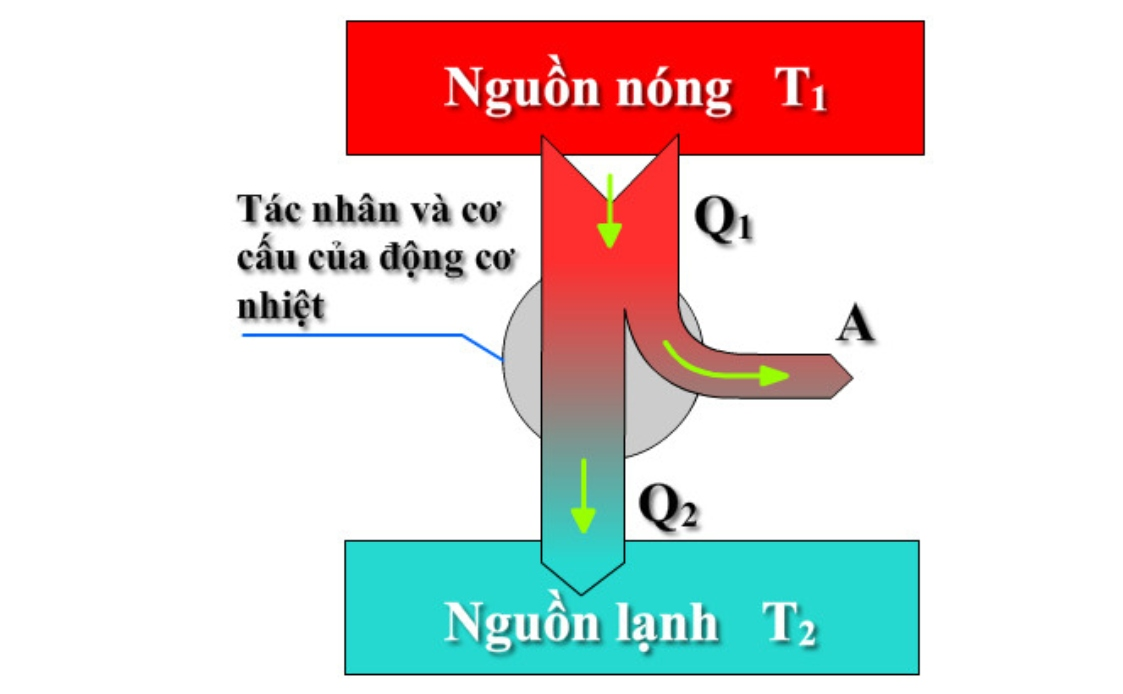
\includegraphics[scale=0.25]{figs/VN12-Y24-PH-SYL-007-1}
				\end{center}
				\item \textbf{Hiệu suất của động cơ nhiệt}\\
				$$H=\dfrac{A}{Q_1}=\dfrac{Q_1-Q_2}{Q_1}=1-\dfrac{Q_2}{Q_1}.$$
\begin{luuy}
	Động cơ nhiệt không thể chuyển đổi toàn bộ nhiệt lượng nhận được thành công $\left(H<1\right)$.\\
					Hiệu suất cực đại của động cơ nhiệt:
					$$H_\text{max}=\dfrac{T_1-T_2}{T_1}.$$
\end{luuy}
			\end{itemize}
\end{dang}
% =======================================
\begin{vd}
Một động cơ nhiệt làm việc sau một thời gian thì tác nhân đã nhận từ nguồn nóng nhiệt lượng $Q_1=\SI{1.5E6}{\joule}$, truyền cho nguồn lạnh nhiệt lượng $Q_2=\SI{1.2E6}{\joule}$. Hiệu suất thực của động cơ nhiệt này là bao nhiêu?
	\loigiai{
			Hiệu suất thực của động cơ nhiệt:
			$$H=1-\dfrac{Q_2}{Q_1}=1-\dfrac{\SI{1.2E6}{\joule}}{\SI{1.5E6}{\joule}}=\SI{20}{\percent}.$$
		}
\end{vd}
% ===============================================
\begin{vd}
Máy hơi nước công suất $\SI{10}{\kilo\watt}$ tiêu thụ $\SI{10}{\kilogram}$ than đá trong $\SI{1}{\text{giờ}}$. Biết hơi nước vào và ra cylanh có nhiệt độ $\SI{227}{\celsius}$ và $\SI{100}{\celsius}$. Năng suất toả nhiệt của than đá là $\SI{3.6E7}{\joule/\kilogram}$. Tính hiệu suất thực của máy và của một động cơ nhiệt lí tưởng làm việc với nhiệt độ nguồn nóng và nguồn lạnh nói trên.
\loigiai{
			Hiệu suất của một động cơ nhiệt lí tưởng hoạt động giữa hai nguồn nhiệt $\SI{227}{\celsius}$ và $\SI{100}{\celsius}$:
			$$T_1=t_1+273=\SI{500}{\kelvin};\quad T_2=t_2+273=\SI{373}{\kelvin}.$$
			$$H_\text{max}=\dfrac{T_1-T_2}{T_1}=\SI{25.4}{\percent}.$$
			Hiệu suất thực của động cơ:
			$$H=\dfrac{A}{Q}=\dfrac{\calP t}{mq}=\dfrac{\left(\SI{10E3}{\watt}\right)\cdot\left(\SI{3600}{\second}\right)}{\left(\SI{10}{\kilogram}\right)\cdot\left(\SI{3.6E7}{\joule/\kilogram}\right)}=\SI{10}{\percent}.$$}

\end{vd}
\subsection{BÀI TẬP TRẮC NGHIỆM}
\Opensolutionfile{ans}[ans/G12Y24B6TN]
% ===================================================================
\begin{ex}
	Một động cơ nhiệt lí tưởng thực hiện một công $\SI{5}{\kilo\joule}$ đồng thời truyền cho nguồn lạnh nhiệt lượng $\SI{15}{\kilo\joule}$. Hiệu suất của động cơ nhiệt này là
	\choice
	{$\SI{33.33}{\percent}$}
	{$\SI{75}{\percent}$}
	{\True $\SI{25}{\percent}$}
	{$\SI{66.67}{\percent}$}
	\loigiai{$$H=\dfrac{A}{Q_1}=\dfrac{A}{Q_2+A}=\SI{25}{\percent}.$$
	}
\end{ex}
% ===================================================================
\begin{ex}
	Một động cơ nhiệt làm việc giữa hai nguồn nhiệt. Nhiệt lượng tác nhân nhận của nguồn nóng trong một chu trình là $\SI{2400}{\joule}$. Hiệu suất của động cơ nhiệt là $\SI{25}{\percent}$. Nhiệt lượng tác nhân truyền cho nguồn lạnh trong một chu trình là
	
	\choice
	{$\SI{1200}{\joule}$}
	{$\SI{2400}{\joule}$}
	{$\SI{600}{\joule}$}
	{\True $\SI{1800}{\joule}$}
	\loigiai{$$H=1-\dfrac{Q_2}{Q_1}\Rightarrow Q_2=\SI{1800}{\joule}.$$
	}
\end{ex}
% ===================================================================
\begin{ex}
	Một động cơ nhiệt nhả cho nguồn lạnh $\SI{80}{\percent}$ nhiệt lượng mà nó thu được từ nguồn nóng. Hiệu suất của động cơ nhiệt này là
	
	\choice
	{\True $\SI{20}{\percent}$}
	{$\SI{37}{\percent}$}
	{$\SI{50}{\percent}$}
	{$\SI{80}{\percent}$}
	\loigiai{Hiệu suất của động cơ nhiệt:
		$$H=1-\dfrac{Q_2}{Q_1}=\SI{20}{\percent}.$$
	}
\end{ex}
% ===================================================================
\begin{ex}
	Người ta phải tốn $\SI{150}{\gram}$ dầu hoả để đun sôi được $\SI{4.5}{\text{lít}}$ nước ở nhiệt độ ban đầu $\SI{20}{\celsius}$. Cho biết khối lượng riêng của nước là $\SI{1}{\kilogram/\text{lít}}$, nhiệt dung riêng của nước là $\SI{4200}{\joule/\left(\kilogram\cdot\kelvin\right)}$, năng suất toả nhiệt của dầu hoả là $\SI{44E6}{\joule/\kilogram}$. Hiệu suất của bếp đun là
	
	\choice
	{\True $\SI{22.9}{\percent}$}
	{$\SI{2.29}{\percent}$}
	{$\SI{12.9}{\percent}$}
	{$\SI{26.9}{\percent}$}
	\loigiai{Hiệu suất của bếp đun:
		$$H=\dfrac{m_\text{n}c\Delta t}{m_\text{d}q}=\SI{22.9}{\percent}.$$
	}
\end{ex}
% ===================================================================
\begin{ex}
	Để đun sôi một lượng nước bằng bếp dầu có hiệu suất $\SI{30}{\percent}$, phải dùng hết 1 lít dầu. Để đun sôi cũng lượng nước trên với bếp dầu có hiệu suất $\SI{20}{\percent}$ thì phải dùng
	
	\choice
	{2 lít dầu}
	{0,5 lít dầu}
	{\True 1,5 lít dầu}
	{3 lít dầu}
	\loigiai{$$V_2=\dfrac{V_1H_1}{H_2}=\SI{1.5}{\liter}.$$
	}
\end{ex}
% ===================================================================
\begin{ex}
	Khi dùng lò có hiệu suất $H_1$ để làm chảy một lượng quặng, phải đốt hết $\xsi{m_1}{\left(\kilogram\right)}$ nhiên liệu có năng suất toả nhiệt $q_1$. Nếu dùng lò có hiệu suất $H_2$ để làm chảy lượng quặng trên thì phải đốt hết $m_2=\xsi{3m_1}{\left(\kilogram\right)}$ nhiên liệu có năng suất toả nhiệt $q_2=0,5q_1$. Hệ thức liên hệ giữa $H_1$ và $H_2$ là
	
	\choice
	{$H_1=H_2$}
	{$H_1=2H_2$}
	{$H_1=3H_2$}
	{\True $H_1=1,5H_2$}
	\loigiai{$$H=\dfrac{Q}{mq}$$
		$$\Rightarrow \dfrac{H_1}{H_2}=\dfrac{m_2q_2}{m_1q_1}=\dfrac{3}{2}.$$}
\end{ex}
% ===================================================================
\begin{ex}
	Một động cơ nhiệt có hiệu suất $\SI{25}{\percent}$ và công suất $\SI{30}{\kilo\watt}$. Nhiệt lượng mà động cơ toả ra cho nguồn lạnh trong 5 giờ làm việc liên tục là
	
	\choice
	{$\SI{176E7}{\joule}$}
	{$\SI{194E7}{\joule}$}
	{$\SI{213E7}{\joule}$}
	{\True $\SI{162E7}{\joule}$}
	\loigiai{$$H=\dfrac{A}{A+Q_2}=\dfrac{\calP t}{\calP t+Q_2}\Rightarrow Q_2=\SI{162E7}{\joule}.$$}
\end{ex}
% ===================================================================
\begin{ex}
	Một đầu máy diezen xe lửa có công suất $\SI{3E6}{\watt}$ và có hiệu suất $\SI{25}{\percent}$. Cho biết năng suất toả nhiệt của nhiên liệu là $\SI{4.2E7}{\joule/\kilogram}$. Nếu đầu máy chạy hết công suất thì khối lượng nhiên liệu tiêu thụ trong mỗi giờ \textbf{gần giá trị nào nhất} sau đây?
	
	\choice
	{$\SI{2489}{\kilogram}$}
	{$\SI{1429}{\kilogram}$}
	{\True $\SI{1028}{\kilogram}$}
	{$\SI{1056}{\kilogram}$}
	\loigiai{Khối lượng nhiên liệu tiêu thụ trong 1 giờ khi động cơ xe lửa hoạt động hết công suất:
		$$m=\dfrac{\calP t}{qH}\approx\SI{1028.57}{\kilogram}.$$
	}
\end{ex}
% ===================================================================
\begin{ex}
	Một máy bơm sau khi tiêu thụ hết $\SI{8}{\kilogram}$ dầu thì đưa được $\SI{700}{\meter^3}$ nước lên cao $\SI{8}{\meter}$. Biết năng suất toả nhiệt của dầu dùng cho  máy bơm này là $\SI{4.6E7}{\joule/\kilogram}$. Xem rằng nước được đưa lên cao một cách đều đặn, khối lượng riêng của nước $\SI{1000}{\kilogram/\meter^3}$, gia tốc trọng trường $g=\SI{10}{\meter/\second^2}$. Hiệu suất của máy bơm là
	
	\choice
	{\True $\SI{15.22}{\percent}$}
	{$\SI{24.46}{\percent}$}
	{$\SI{1.52}{\percent}$}
	{$\SI{2.45}{\percent}$}
	\loigiai{Hiệu suất máy bơm:
		$$H=\dfrac{\rho Vgh}{qm_\text{d}}\approx\SI{15.22}{\percent}.$$
	}
\end{ex}
% ===================================================================
\begin{ex}
	Một ô tô chạy $\SI{100}{\kilo\meter}$ với lực kéo không đổi $\SI{700}{\newton}$ thì tiêu thụ hết $\SI{6}{\text{lít}}$ xăng. Biết năng suất toả nhiệt của xăng là $\SI{4.6E7}{\joule/\kilogram}$, khối lượng riêng của xăng là $\SI{700}{\kilogram/\meter^3}$. Hiệu suất của động cơ ô tô là
	
	\choice
	{$\SI{25}{\percent}$}
	{\True $\SI{36}{\percent}$}
	{$\SI{0.36}{\percent}$}
	{$\SI{17.75}{\percent}$}
	\loigiai{Hiệu suất của động cơ ô tô:
		$$H=\dfrac{A}{Q}=\dfrac{Fs}{\rho_\text{xăng}Vq}=\SI{36.23}{\percent}.$$
	}
\end{ex}
% ===================================================================
\begin{ex}
	Một nhà máy điện tiêu thụ $\SI{0.35}{\kilogram}$ nhiên liệu cho mỗi $\SI{1}{\kilo\watt\hour}$ điện năng. Cho biết năng suất toả nhiệt của nhiên liệu trên là $\SI{42}{\mega\joule/\kilogram}$. Hiệu suất của động cơ nhiệt dùng trong nhà máy điện \textbf{gần nhất} với giá trị nào sau đây?
	
	\choice
	{$\SI{38}{\percent}$}
	{$\SI{15}{\percent}$}
	{$\SI{20}{\percent}$}
	{\True $\SI{24}{\percent}$}
	\loigiai{Hiệu suất của động cơ nhiệt dùng trong nhà máy:
		$$H=\dfrac{A}{Q_\text{tp}}=\dfrac{\left(\SI{E3}{\watt}\right)\cdot\left(\SI{3600}{\second}\right)}{\left(\SI{0.35}{\kilogram}\right)\cdot\left(\SI{42E6}{\joule/\kilogram}\right)}\approx\SI{24.5}{\percent}.$$}
\end{ex}
% ===================================================================
\begin{ex}
	Một chiếc xe máy hoạt động với công suất $\SI{3.2}{\kilo\watt}$ và chuyển động đều với tốc độ $\SI{45}{\kilo\meter/\hour}$. Hiệu suất của động cơ là $\SI{25}{\percent}$, năng suất toả nhiệt của xăng là $\SI{4.6E7}{\joule/\kilogram}$, khối lượng riêng của xăng là $\SI{700}{\kilogram/\meter^3}$. Với 2 lít xăng thì xe máy đi được bao nhiêu $\si{\kilo\meter}$?
	
	\choice
	{$\SI{100.6}{\kilo\meter}$}
	{\True $\SI{63}{\kilo\meter}$}
	{$\SI{45}{\kilo\meter}$}
	{$\SI{54}{\kilo\meter}$}
	\loigiai{Thời gian động cơ xe máy hoạt động được khi tiêu thụ $\SI{2}{\text{lít}}$ xăng:
		$$t=\dfrac{q\rho V}{\calP}\cdot H=\SI{5031.25}{\second}=\SI{1.39}{\hour}.$$
		Quãng đường xe máy đi được:
		$$s=vt\approx\SI{62.89}{\kilo\meter}.$$
	}
\end{ex}
% ===================================================================
\begin{ex}
	Một động cơ ô tô hoạt động với công suất $\SI{20}{\kilo\watt}$ và ô tô chuyển động đều với tốc độ $\SI{72}{\kilo\meter/\hour}$. Ô tô tiêu thụ $\SI{20}{\text{lít}}$ xăng thì chạy được quãng đường $\SI{200}{\kilo\meter}$. Biết khối lượng riêng của xăng là $\SI{700}{\kilogram/\meter^3}$, năng suất toả nhiệt của xăng là $\SI{4.6E7}{\joule/\kilogram}$. Hiệu suất của động cơ ô tô khi đó là
	
	\choice
	{\True $\SI{31}{\percent}$}
	{$\SI{61}{\percent}$}
	{$\SI{63}{\percent}$}
	{$\SI{36}{\percent}$}
	\loigiai{Hiệu suất của ô tô:
		$$H=\dfrac{\calP\cdot\dfrac{s}{v}}{\rho Vq}\approx\SI{31.05}{\percent}.$$
	}
\end{ex}
% ===================================================================
\begin{ex}
	Dùng một bếp dầu hoả để đun sôi 2 lít nước từ $\SI{15}{\celsius}$ thì mất $\SI{10}{\text{phút}}$. Biết rằng chỉ có $\SI{40}{\percent}$ nhiệt lượng do dầu toả ra làm nóng nước. Lấy nhiệt dung riêng của nước là $\SI{4190}{\joule/\left(\kilogram\cdot\kelvin\right)}$, năng suất toả nhiệt của dầu hoả là $\SI{46E6}{\joule/\kilogram}$, khối lượng riêng của nước là $\SI{1}{\gram/\centi\meter^3}$. Lượng dầu hoả cần dùng trong mỗi phút là
	\choice
	{$\SI{0.619}{\gram}$}
	{$\SI{0.619}{\kilogram}$}
	{\True $\SI{3.87}{\gram}$}
	{$\SI{3.87}{\kilogram}$}
	\loigiai{Khối lượng dầu cần dùng trong mỗi phút:
		$$m=\dfrac{Q}{qH}=\dfrac{mc\Delta t}{qH}=\SI{3.87E-3}{\kilogram}=\SI{3.87}{\gram}.$$
	}
\end{ex}
% ===================================================================
\begin{ex}
	Người ta cần nấu chảy 10 tấn đồng trong lò nung dùng dầu làm nhiên liệu đốt. Cho biết nhiệt độ ban đầu, nhiệt độ nóng chảy, nhiệt dung riêng và nhiệt nóng chảy riêng của đồng lần lượt là $\SI{13}{\celsius}$, $\SI{1083}{\celsius}$, $\SI{380}{\joule/\left(\kilogram\cdot\kelvin\right)}$, $\SI{1.8E5}{\joule/\kilogram}$. Nhiệt lượng toả ra khi đốt cháy $\SI{1}{\kilogram}$ dầu là $\SI{4.6E7}{\joule/\kilogram}$. Nếu hiệu suất nung của lò là $\SI{30}{\percent}$ thì khối lượng dầu cần dùng là
	\choice
	{\True $\SI{425.1}{\kilogram}$}
	{$\SI{127.5}{\kilogram}$}
	{$\SI{38.3}{\kilogram}$}
	{$\SI{432.2}{\kilogram}$}
	\loigiai{Nhiệt lượng đồng cần thu vào để nóng chảy hoàn toàn:
		$$Q=mc\Delta t+m\lambda=\SI{58.66E8}{\joule}.$$
		Khối lượng xăng cần dùng:
		$$m=\dfrac{Q}{qH}=\SI{425.1}{\kilogram}.$$
	}
\end{ex}
% ===================================================================
\begin{ex}
Một ấm nhôm có khối lượng $m_\text{b}=\SI{600}{\gram}$ chứa $V=\SI{1.5}{\text{lít}}$ nước ở $t_1=\SI{20}{\celsius}$, sau đó đun bằng bếp điện. Sau thời gian $t=\SI{35}{\text{phút}}$ thì đã có $\SI{20}{\percent}$ khối lượng nước đã hoá hơi ở nhiệt độ sôi $t_2=\SI{100}{\percent}$. Biết rằng, $\SI{75}{\percent}$ nhiệt lượng mà bếp cung cấp được dùng vào việc đun nước. Cho biết nhiệt dung riêng của nước là $c_\text{n}=\SI{4190}{\joule/\left(\kilogram\cdot\kelvin\right)}$, của nhôm là $c_\text{b}=\SI{880}{\joule/\left(\kilogram\cdot\kelvin\right)}$, nhiệt hoá hơi riêng của nước ở $\SI{100}{\celsius}$ là $L=\SI{2.26E6}{\joule/\kilogram}$, khối lượng riêng của nước là $D=\SI{1}{\kilogram/\text{lít}}$. Công suất cung cấp nhiệt của bếp điện \textbf{gần giá trị nào nhất} sau đây?	
	\choice
	{\True $\SI{776}{\watt}$}
	{$\SI{796}{\watt}$}
	{$\SI{786}{\watt}$}
	{$\SI{876}{\watt}$}
	\loigiai{Khối lượng nước $$m_\text{n}=VD=\SI{1.5}{\kilogram}.$$
		Tổng nhiệt lượng nước và ấm thu vào:
		$$Q=\left(m_\text{n}c_\text{n}+m_\text{b}c_\text{b}\right)\cdot\left(t_2-t_1\right)+\SI{20}{\percent}m_\text{n}L=\SI{1223040}{\joule}.$$
		Điện năng tiêu thụ của ấm:
		$$A=\dfrac{Q}{H}=\SI{1630720}{\joule}.$$
		Công suất của ấm điện:
		$$\calP=\dfrac{A}{t}\approx\SI{776.5}{\watt}.$$	}
\end{ex}
\Closesolutionfile{ans}
	\subsection{TRẮC NGHIỆM ĐÚNG/SAI}
	\setcounter{ex}{0}
	% ================================
	\begin{ex}
		\immini{
	Cầu chì là linh kiện được sử dụng để bảo vệ thiết bị và lưới điện tránh sự cố ngắn mạch, hạn chế tình trạng cháy, nổ.
	\begin{enumerate}[label=\alph*)]
		\item Cầu chì có thể bảo vệ mạch điện dựa trên sự phụ thuộc của điện trở kim loại theo nhiệt độ.
		\item Dây chảy trong cầu chì thường được làm từ kim loại có nhiệt độ nóng chảy cao.
		\item Khi cường độ dòng điện qua mạch tăng vượt hạn, dây chì sẽ nóng chảy trước.
		\item Khi dây chảy trong cầu chì bị đứt, ta có thể nối cầu chì bằng dây sắt.
	\end{enumerate}	
	}{
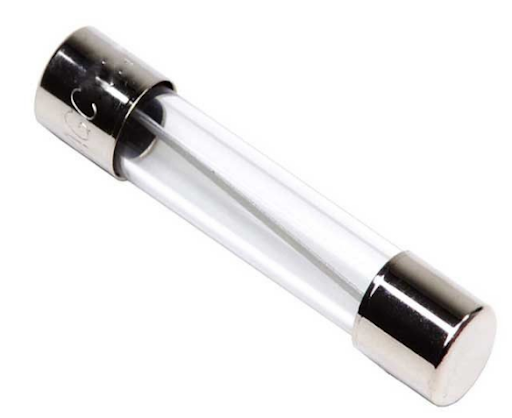
\includegraphics[scale=0.2]{figs/VN12-Y24-PH-SYL-007P-1}
}
\loigiai{
\begin{enumerate}[label=\alph*)]
	\item Sai. Khi dòng điện qua mạch vượt hạn, dây chảy trong cầu chì nóng chảy trước và là hở mạch.
	\item Sai. Dây chảy được làm từ kim loại có nhiệt độ nóng chảy thấp.
	\item Đúng.
	\item Sai. Sắt là kim loại có nhiệt độ nóng chảy cao, khi cường độ dòng điện tăng quá lớn nhưng dây sắt nóng chảy chậm nên không bảo vệ được mạch điện.
\end{enumerate}
}
		\end{ex}
	\subsection{BÀI TẬP TỰ LUẬN}
	\setcounter{ex}{0}
% ===================================================================
\begin{ex}
	Một bếp dầu đun sôi 1 lít nước đựng trong ấm bằng nhôm khối lượng $m_2=\SI{300}{\gram}$ thì sau thời gian $t_1=\SI{10}{\minute}$ nước sôi. Nếu dùng bếp trên để đun 2 lít nước trong cùng điều kiện thì sau bao lâu nước sôi? Cho nhiệt dung riêng của nước và nhôm lần lượt là $c_1=\SI{4200}{\joule/\left(\kilogram\cdot\kelvin\right)}$, $c_2=\SI{880}{\joule/\left(\kilogram\cdot\kelvin\right)}$. Biết nhiệt do bếp dầu cung cấp một cách đều đặn.
	\loigiai{Vì bếp dầu cung cấp nhiệt lượng một cách đều đặn nên
		$$\dfrac{t_2}{t_1}=\dfrac{\left(m_2c_2+m'_1c_1\right)\Delta t}{\left(m_2c_2+m_1c_1\right)\Delta t}=\dfrac{m_2c_2+m'_1c_1}{m_2c_2+m_1c_1}\Rightarrow t_2\approx\SI{19.4}{\minute}.$$}
\end{ex}
% ===================================================================
\begin{ex}
	Khi thả một quả cầu nhôm khối lượng $\SI{500}{\gram}$ vào $\SI{2}{\kilogram}$ nước ở $\SI{25}{\celsius}$ thì nhiệt độ của chúng sau khi cân bằng nhiệt là $\SI{30}{\celsius}$. Hỏi nhiệt độ ban đầu của quả cầu nhôm là bao nhiêu? Biết nhiệt lượng hao phí trong trường hợp này bằng $\SI{20}{\percent}$ nhiệt lượng do nước thu vào. Biết nhiệt dung riêng của nhôm là $\SI{880}{\joule/\left(\kilogram\cdot\kelvin\right)}$, nhiệt dung riêng của nước là $\SI{4200}{\joule/\left(\kilogram\cdot\kelvin\right)}$. Bỏ qua sự hoá hơi của nước ngay khi tiếp xúc với quả cầu.
	
	\loigiai{Khi hệ cân bằng nhiệt, tổng nhiệt lượng trao đổi trong hệ bằng 0:
		\begin{eqnarray*}
			&&Q_1+Q_2+Q_\text{hp}=0\\
			&\Leftrightarrow& m_1C_1\left(t_\text{cb}-t_1\right)+1,2m_2C_2\left(t_\text{cb}-t_2\right)=0\\
			&\Rightarrow& t_1\approx\SI{144.55}{\celsius}.
	\end{eqnarray*}}
\end{ex}
% ===================================================================
\begin{ex}
	Động cơ nhiệt lí tưởng làm việc giữa hai nguồn nhiệt $\SI{27}{\celsius}$ và $\SI{127}{\celsius}$. Nhiệt lượng tác nhân nhận từ nguồn nóng trong một chu trình là $\SI{2400}{\joule}$. Tính:
	\begin{enumerate}[label=\alph*)]
		\item hiệu suất của động cơ.
		\item công thực hiện trong một chu trình.
		\item nhiệt lượng truyền cho nguồn lạnh trong một chu trình.
	\end{enumerate}
	
	\loigiai{\begin{enumerate}[label=\alph*)]
			\item $H=\dfrac{T_1-T_2}{T_1}=\SI{25}{\percent}.$
			\item $A=H\cdot Q_1=\SI{600}{\joule}$.
			\item $Q_2=Q_1-A=\SI{1800}{\joule}$.
		\end{enumerate}
	}
\end{ex}
% ===================================================================
\begin{ex}
	Máy hơi nước công suất $\SI{1}{\kilo\watt}$ tiêu thụ $\SI{10}{\kilogram}$ than đá trong 1 giờ. Biết hơi nước vào và ra cylanh có nhiệt độ $\SI{227}{\celsius}$ và $\SI{100}{\celsius}$. Năng suất toả nhiệt của than đá là $\SI{3.6E7}{\joule/\kilogram}$. Tính hiệu suất thực của máy và của một động cơ nhiệt lý tưởng làm việc giữa hai nhiệt độ nói trên.
	
	\loigiai{Hiệu suất của máy:
		$$H=\dfrac{A}{Q}=\dfrac{\calP t}{mq}=\SI{10}{\percent}.$$
		Hiệu suất của động cơ nhiệt lí tưởng:
		$$H_\text{max}=\dfrac{T_1-T_2}{T_1}=\SI{25.4}{\percent}.$$
	}
\end{ex}
% ===================================================================
\begin{ex}
	Một động cơ hơi nước lí tưởng là động cơ nhiệt có hiệu suất cực đại, hoạt động với nguồn nóng là lò hơi có nhiệt độ $\SI{500}{\kelvin}$. Nước được đưa vào lò hơi và được đun nóng để chuyển thể thành hơi nước. Hơi nước này làm piston chuyển động. Nhiệt độ của nguồn lạnh là nhiệt độ bên ngoài của không khí, bằng $\SI{300}{\kelvin}$.
	\begin{enumerate}[label=\alph*)]
		\item Tính công của động cơ hơi nước thực hiện khi lò hơi cung cấp cho tác nhân một nhiệt lượng bằng $\SI{6.5E3}{\joule}$.
		\item Giả sử muốn tăng hiệu suất này lên $\SI{45}{\percent}$ phải tăng nhiệt độ lò hơi lên một lượng bằng bao nhiêu?
	\end{enumerate}
	
	\loigiai{\begin{enumerate}[label=\alph*)]
			\item $H=\dfrac{A}{Q_1}=\dfrac{T_1-T_2}{T_1}\Rightarrow A=\SI{2600}{\joule}$.
			\item $H_\text{max}=\dfrac{T_1-T_2}{T_1}\Rightarrow T_1\approx\SI{545.46}{\kelvin}.$
		\end{enumerate}
	}
\end{ex}
% ===================================================================
\begin{ex}
	Búa máy 10 tấn rơi từ độ cao $\SI{2.3}{\meter}$ xuống một cọc sắt khối lượng $\SI{200}
	{\kilogram}$. Biết $\SI{40}{\percent}$ động năng của búa biến thành nhiệt làm nóng cọc sắt. Hỏi búa rơi bao nhiêu lần thì cọc tăng nhiệt độ thêm $\SI{20}{\celsius}$. Cho rằng cọc không toả nhiệt ra môi trường và nhiệt dung riêng của sắt là $\SI{0.46}{\kilo\joule/\left(\kilogram\cdot\kelvin\right)}$.
	\loigiai{\begin{itemize}
			\item Động năng của búa ngay trước khi va chạm với cọc: $W_\text{đ}=Mgh$.
			\item Nhiệt lượng cọc thu được sau mỗi lần búa rơi: $Q_0=0,4W_\text{đ}=0,4Mgh$.
			\item Nhiệt lượng cọc thu được sau $n$ lần búa rơi: $Q=nQ_0=mc\Delta t$.
		\end{itemize}
		Suy ra:
		$$n=\dfrac{mc\Delta t}{0,4Mgh}=20.$$
	}
\end{ex}

	
\newpage\section*{ÔN TẬP CHƯƠNG I}
\subsection{Câu trắc nghiệm nhiều phương án lựa chọn}
\textit{Thí sinh trả lời từ câu 1 đến câu 18. Mỗi câu hỏi thí sinh chọn một phương án}
\Opensolutionfile{ans}[ans/G12Y24B7TN]
% ===================================================================
\begin{ex}
	Quy ước dấu nào sau đây phù hợp với định luật I của nhiệt động lực học?
	\choice
	{Vật nhận công $A<0$; vật nhận nhiệt $Q<0$}
	{Vật thực hiện công $A>0$; vật truyền nhiệt lượng $Q<0$}
	{\True Vật nhận công $A>0$; vật nhận nhiệt lượng $Q>0$}
	{Vật thực hiện công $A>0$; vật truyền nhiệt lượng $Q>0$}
	\loigiai{}
\end{ex}
% ===================================================================
\begin{ex}
	Ở nhiệt độ phòng, chất nào sau đây không tồn tại ở thể lỏng?
	\choice
	{Rượu}
	{\True Nhôm}
	{Thuỷ ngân}
	{Nước}
	\loigiai{}
\end{ex}
% ===================================================================
\begin{ex}
	Vật nào sau đây có cấu trúc tinh thể?
	\choice
	{\True Chiếc cốc thuỷ tinh}
	{Hạt muối ăn}
	{Viên kim cương}
	{Miếng thạch anh}
	\loigiai{}
\end{ex}
% ===================================================================
\begin{ex}
Điều nào sau đây là \textbf{sai} khi nói về sự đông đặc?	
	\choice
	{Sự đông đặc là quá trình chuyển từ thể lỏng sang thể rắn}
	{\True Với một chất rắn, nhiệt độ đông đặc luôn nhỏ hơn nhiệt độ nóng chảy}
	{Trong suốt quá trình đông đặc, nhiệt độ của vật không thay đổi}
	{Nhiệt độ đông đặc của các chất thay đổi theo áp suất bên ngoài}
	\loigiai{}
\end{ex}
% ===================================================================
\begin{ex}
	Biểu thức nào sau đây là biểu thức chuyển đổi đúng đơn vị nhiệt độ từ $\si{\celsius}$ sang thang $\si{\kelvin}$?
	\choice
	{\True $\xsi{T}{\left(\si{\kelvin}\right)}=\xsi{t}{\left(\si{\celsius}\right)}+273$}
	{$\xsi{T}{\left(\si{\kelvin}\right)}=\xsi{t}{\left(\si{\celsius}\right)}-273$}
	{$\xsi{T}{\left(\si{\kelvin}\right)}=\dfrac{9}{5}\xsi{t}{\left(\si{\celsius}\right)}+273$}
	{$\xsi{T}{\left(\si{\kelvin}\right)}=\dfrac{9}{5}\xsi{t}{\left(\si{\celsius}\right)}-273$}
	\loigiai{}
\end{ex}
% ===================================================================
\begin{ex}
	Trong thang nhiệt độ Celsius, nhiệt độ không tuyệt đối là
	\choice
	{$\SI{100}{\celsius}$}
	{\True $\SI{-273}{\celsius}$}
	{$\SI{0}{\celsius}$}
	{$\SI{-32}{\celsius}$}
	\loigiai{}
\end{ex}
% ===================================================================
\begin{ex}
	Đơn vị nhiệt nóng chảy riêng của vật rắn là
	\choice
	{$\si{\joule}$}
	{$\si{\joule/\kelvin}$}
	{\True $\si{\joule/\kilogram}$}
	{$\si{\joule/\left(\kilogram\cdot\kelvin\right)}$}
	\loigiai{}
\end{ex}

% ===================================================================
\begin{ex}
	Kết luận nào sau đây \textbf{không đúng} với thang nhiệt độ Celsius?
	\choice
	{Đơn vị đo nhiệt độ là $\si{\celsius}$}
	{Chọn mốc nhiệt độ nước đá đang tan ở áp suất $\SI{1}{atm}$ là $\SI{0}{\celsius}$}
	{Chọn mốc nhiệt độ nước sôi ở áp suất $\SI{1}{atm}$ là $\SI{100}{\celsius}$}
	{\True $\SI{1}{\celsius}$ tương ứng với $\SI{273}{\kelvin}$}
	\loigiai{}
\end{ex}
% ===================================================================
\begin{ex}
	Nhiệt hoá hơi riêng của nước là $\SI{2.3E6}{\joule/\kilogram}$. Phát biểu nào dưới đây là \textbf{đúng}?
	\choice
	{\True Mỗi kilogram nước cần thu một lượng nhiệt $\SI{2.3E6}{\joule}$ để bay hơi hoàn toàn ở nhiệt độ sôi và áp suất chuẩn}
	{Mỗi kilogram nước cần thu một lượng nhiệt $\SI{2.3E6}{\joule}$ để bay hơi hoàn toàn}
	{Mỗi kilogram nước cần toả ra một lượng nhiệt $\SI{2.3E6}{\joule}$ để bay hơi hoàn toàn ở nhiệt độ sôi}
	{Một lượng nước bất kì cần thu một lượng nhiệt là $\SI{2.3E6}{\joule}$ để bay hơi hoàn toàn}
	\loigiai{}
\end{ex}
% ===================================================================
\begin{ex}
	Hãy tìm ý \textbf{không đúng} với mô hình động học phân tử.
	\choice
	{\True Tốc độ chuyển động của các phân tử cấu tạo nên vật càng lớn thì thể tích của vật càng lớn}
	{Các chất được cấu tạo từ các hạt riêng biệt gọi là phân tử}
	{Các phân tử chuyển động không ngừng}
	{Giữa các phân tử có lực tương tác gọi là lực liên kết phân tử}
	\loigiai{}
\end{ex}
% ===================================================================
\begin{ex}
	Điểm đóng băng và điểm sôi của nước theo thang nhiệt độ Kelvin là
	\choice
	{\True $\SI{273}{\kelvin}$ và $\SI{373}{\kelvin}$}
	{$\SI{0}{\kelvin}$ và $\SI{100}{\kelvin}$}
	{$\SI{73}{\kelvin}$ và $\SI{37}{\kelvin}$}
	{$\SI{32}{\kelvin}$ và $\SI{212}{\kelvin}$}
	\loigiai{}
\end{ex}
% ===================================================================
\begin{ex}
	Người ta cung cấp cho khí trong một cylanh nằm ngang nhiệt lượng $\SI{2}{\joule}$. Đồng thời nén piston một đoạn $\SI{5}{\centi\meter}$ với một lực có độ lớn là $\SI{20}{\newton}$. Độ biến thiên nội năng của khí là
	\choice
	{\True $\SI{3}{\joule}$}
	{$\SI{1}{\joule}$}
	{$\SI{-1}{\joule}$}
	{$\SI{-3}{\joule}$}
	\loigiai{$$\Delta U=Q+A=Q+F\cdot s=\SI{3}{\joule}.$$
	}
\end{ex}
% ===================================================================
\begin{ex}
	Nhiệt lượng cần cung cấp cho $\SI{0.5}{\kilogram}$ nước ở $\SI{0}{\celsius}$ đến khi nó sôi là bao nhiêu? Biết nhiệt dung riêng của nước là $\SI{4180}{\joule/\left(\kilogram\cdot\kelvin\right)}$.
	\choice
	{$\SI{5E5}{\joule}$}
	{$\SI{3E5}{\joule}$}
	{$\SI{4.18E5}{\joule}$}
	{\True $\SI{2.09E5}{\joule}$}
	\loigiai{$$Q=mc\Delta t=\SI{2.09E5}{\joule}.$$
	}
\end{ex}
% ===================================================================
\begin{ex}
	Biết nhiệt dung riêng của nước là $\SI{4200}{\joule/\left(\kilogram\cdot\kelvin\right)}$, nhiệt nóng chảy riêng của nước đá là $\SI{3.4E5}{\joule/\kilogram}$. Nhiệt lượng cần cung cấp cho $\SI{2}{\kilogram}$ nước đá ở nhiệt độ $\SI{0}{\celsius}$ là bao nhiêu để tăng nhiệt độ lên $\SI{60}{\celsius}$ là
	\choice
	{$\SI{0.72E6}{\joule}$}
	{\True $\SI{1.184E6}{\joule}$}
	{$\SI{2.254E6}{\joule}$}
	{$\SI{1.548E6}{\joule}$}
	\loigiai{Nhiệt lượng cần cung cấp cho $\SI{2}{\kilogram}$ nước đá ở nhiệt độ $\SI{0}{\celsius}$ là bao nhiêu để chuyển lên nhiệt độ $\SI{60}{\celsius}$ là
		$$Q=m\lambda+mc\Delta t=\SI{1.184E6}{\joule}.$$
	}
\end{ex}
% ===================================================================
\begin{ex}
Một lượng nước và một lượng rượu có thể tích bằng nhau, được cung cấp các nhiệt lượng tương ứng là $Q_1$ và $Q_2$. Biết khối lượng riêng của nước là $\SI{1000}{\kilogram/\meter^3}$ và của rượt là $\SI{800}{\kilogram/\meter^3}$, nhiệt dung riêng của nước và rượu lần lượt là $\SI{4200}{\joule/\left(\kilogram\cdot\kelvin\right)}$ và $\SI{2500}{\joule/\left(\kilogram\cdot\kelvin\right)}$. Để độ tăng nhiệt độ của nước và rượu bằng nhau thì
	\choice
	{$Q_1=Q_2$}
	{$Q_1=1,68Q_2$}
	{$Q_1=1,25Q_2$}
	{\True $Q_1=2,10Q_2$}
	\loigiai{$$\dfrac{Q_1}{Q_2}=\dfrac{m_1c_1}{m_2c_2}=\dfrac{\rho_1c_1}{\rho_2c_2}=2,1.$$
	}
\end{ex}
% ===================================================================
\begin{ex}
	Một ấm đun nước bằng nhôm có khối lượng $\SI{400}{\gram}$, chứa 3 lít nước được đun trên bếp. Khi nhận nhiệt lượng $\SI{740}{\kilo\joule}$ thì ấm đạt đến nhiệt độ $\SI{80}{\celsius}$. Biết nhiệt dung riêng của nhôm là $\SI{880}{\joule/\left(\kilogram\cdot\kelvin\right)}$, nhiệt dung riêng của nước là $\SI{4190}{\joule/\left(\kilogram\cdot\kelvin\right)}$. Coi nhiệt lượng mà ấm toả ra bên ngoài là không đáng kể. Nhiệt độ ban đầu của ấm và nước là
	\choice
	{$\SI{45.2}{\celsius}$}
	{\True $\SI{22.7}{\celsius}$}
	{$\SI{37.2}{\celsius}$}
	{$\SI{16.7}{\celsius}$}
	\loigiai{$$\Delta t=\dfrac{Q}{m_1c_1+m_2c_2}=\SI{57.27}{\celsius}\Rightarrow t_0=\SI{22.7}{\celsius}.$$
	}
\end{ex}
% ===================================================================
\begin{ex}
	Người ta thực hiện công $\SI{100}{\joule}$ để nén khí trong một cylanh. Biết khí truyền ra môi trường xung quanh nhiệt lượng $\SI{30}{\joule}$ thì độ biến thiên nội năng của khí là
	\choice
	{$\SI{30}{\joule}$}
	{$\SI{130}{\joule}$}
	{\True $\SI{70}{\joule}$}
	{$\SI{100}{\joule}$}
	\loigiai{Độ biến thiên nội năng của khí:
		$$\Delta U=A+Q=\SI{100}{\joule}-\SI{30}{\joule}=\SI{70}{\joule}.$$
	}
\end{ex}
% ===================================================================
\begin{ex}
	Một lượng khí khi bị nung nóng đã tăng thể tích thêm $\SI{0.02}{\meter^3}$ và nội năng biến thiên $\SI{1280}{\joule}$. Biết trong quá trình thay đổi thể tích thì áp suất khí luôn bằng $\SI{2E5}{\pascal}$. Nhiệt lượng đã truyền cho khí là
	\choice
	{$\SI{2720}{\joule}$}
	{$\SI{1280}{\joule}$}
	{\True $\SI{5280}{\joule}$}
	{$\SI{4000}{\joule}$}
	\loigiai{Công khối khí thực hiện trong quá trình dãn nở:
		$$A'=F\cdot \Delta x=pS\Delta x=p\Delta V=\SI{4000}{\joule}.$$
		Nhiệt lượng mà khí đã nhận:
		$$Q=\Delta U-A=\Delta U+A'=\SI{5280}{\joule}.$$
	}
\end{ex}

\Closesolutionfile{ans}
\subsection{CÂU TRẮC NGHIỆM ĐÚNG/SAI}
\setcounter{ex}{0}
\textit{Thí sinh trả lời từ câu 1 đến câu 4. Trong mỗi ý \textbf{a)}, \textbf{b)}, \textbf{c)}, \textbf{d)} ở mỗi câu, thí sinh chọn đúng hoặc sai.}

% ===================================================================
\begin{ex}
Nhận định về các phát biểu sau khi nói về đặc điểm của các chất rắn, lỏng, khí.	
\begin{enumerate}[label=\alph*)]
	\item Các phân tử ở thể lỏng có khoảng cách giữa các phân tử nhỏ hơn khi ở thể rắn.
	\item Các phân tử trong thể khí tự do di chuyển và không bị ràng buộc bởi lực tương tác giữa chúng.
	\item Vật ở thể lỏng không có thể tích riêng, nhưng có hình dạng riêng.
	\item Vật ở thể rắn có thể tích và hình dạng riêng, rất khó nén.
\end{enumerate}
	\loigiai{\begin{enumerate}
			\item Sai. Các phân tử thể lỏng có khoảng cách giữa các phân tử lớn hơn khi ở thể rắn.
			\item Sai. Có lực tương tác phân tử nhưng rất yếu.
			\item Sai. Vật ở thể lỏng có thể tích riêng, nhưng không có hình dạng riêng.
			\item Đúng.
	\end{enumerate}}
\end{ex}
% ===================================================================
\begin{ex}
Nhận định các phát biểu sau về nội năng của một hệ.
\begin{enumerate}[label=\alph*)]
	\item Nội năng của một vật phụ thuộc vào nhiệt độ và thể tích của vật.
	\item Nội năng của một vật thay đổi trong quá trình truyền nhiệt và trong quá trình thực hiện công.
	\item Nội năng của vật A lớn hơn nội năng của vật B thì nhiệt độ của vật A lớn hơn nhiệt độ của vật B.
	\item Nội năng có thể chuyển hoá hoàn toàn thành cơ năng.
\end{enumerate}	
	\loigiai{
		\begin{enumerate}[label=\alph*)]
			\item Đúng.
			\item Đúng.
			\item Sai. Nội năng của hệ không chỉ phụ thuộc vào nhiệt độ của hệ mà còn phụ thuộc vào thể tích của hệ.
			\item Sai. Nội năng của hệ không thể chuyển hoá hoàn toàn thành cơ năng.
	\end{enumerate}}
\end{ex}
% ===================================================================
\begin{ex}
	Một động cơ nhiệt lý tưởng hoạt động giữa hai nguồn nhiệt $\SI{100}{\celsius}$ và $\SI{24.5}{\celsius}$ thì thực hiện công $\SI{2}{\kilo\joule}$.
	\begin{enumerate}[label=\alph*)]
		\item Hiệu suất của động cơ là $\SI{0.2}{}$.
		\item Nhiệt lượng động cơ nhận từ nguồn nóng là $\SI{0.1}{\kilo\joule}$.
		\item Nhiệt lượng động cơ cung cấp cho nguồn lạnh là $\SI{1.9}{\kilo\joule}$.
		\item Để động cơ đạt hiệu suất $\SI{30}{\percent}$ thì phải tăng nhiệt độ nguồn nóng lên $\SI{152}{\celsius}$.
	\end{enumerate}
	
	\loigiai{\begin{enumerate}[label=\alph*)]
			\item Đúng.
			\item Đúng.
			\item Sai. Nhiệt lượng động cơ cung cấp cho nguồn lạnh là $\SI{7.88}{\kilo\joule}$.
			\item Đúng. 
	\end{enumerate}}
\end{ex}
% ===================================================================
\begin{ex}
	Dùng bếp điện để đun một ấm nhôm khối lượng $\SI{600}{\gram}$ đựng $\SI{1.5}{\text{lít}}$ nước ở nhiệt độ $\SI{20}{\celsius}$. Sau $\SI{35}{\minute}$ đã có $\SI{20}{\percent}$ lượng nước trong ấm hoá hơi ở nhiệt độ sôi $\SI{100}{\celsius}$. Biết có $\SI{60}{\percent}$ nhiệt lượng mà bếp toả ra được dùng vào việc đun ấm nước. Cho nhiệt dung riêng của nhôm là $\SI{880}{\joule/\left(\kilogram\cdot\kelvin\right)}$, của nước là $\SI{4200}{\joule/\left(\kilogram\cdot\kelvin\right)}$, nhiệt hoá hơi riêng của nước ở nhiệt độ sôi $\SI{100}{\celsius}$ là $\SI{2.26E6}{\joule/\kilogram}$ và khối lượng riêng của nước là $\SI{1}{\kilogram/\text{lít}}$.
	\begin{enumerate}[label=\alph*)]
		\item Nhiệt lượng cần thiết để đun ấm nước từ $\SI{20}{\celsius}$ đến $\SI{100}{\celsius}$ là $\SI{504000}{\joule}$.
		\item Khối lượng nước đã hoá hơi là $\SI{0.03}{\kilogram}$.
		\item Nhiệt lượng mà bếp điện cung cấp để đun nước đến khi sôi là $\SI{910.4}{\kilo\joule}$.
		\item Nhiệt lượng trung bình mà bếp điện cung cấp cho ấm nước trong mỗi giây là $\SI{582.97}{\joule}$.
	\end{enumerate}
	\loigiai{\begin{enumerate}[label=\alph*)]
			\item Sai. Nhiệt lượng cần thiết để đun sôi ấm nước là $\SI{546240}{\joule}$.
			\item Đúng.
			\item Đúng.
			\item Sai. Nhiệt lượng trung bình mà bếp điện cung cấp cho ấm nước trong mỗi giây là $\SI{971.6}{\joule}$.
		\end{enumerate}
	}
\end{ex}
\subsection{CÂU TRẮC NGHIỆM TRẢ LỜI NGẮN}
\setcounter{ex}{0}
\textit{Thí sinh trả lời từ câu 1 đến câu 6.}
% ===================================================================
\begin{ex}
Giả sử rằng các tuabin ở nhà máy nhiệt điện đã được nâng cấp, dẫn đến sự cải thiện về hiệu suất $\SI{3.32}{\percent}$. Biết rằng trước khi nâng cấp thì hiệu suất của nhà máy điện là $\SI{36}{\percent}$, nhiệt lượng truyền vào động cơ trong một ngày vẫn không đổi và bằng $\SI{2.5E14}{\joule}$. Có thêm bao nhiêu lượng điện năng được sản xuất trong 1 ngày nhờ vào sự nâng cấp trên \textit{(tính theo đơn vị  $\SI{E12}{\joule}$)}?
	\loigiai{$$\Delta A=Q_1\Delta H=\left(\SI{2.5E14}{\joule}\right)\cdot\left(\SI{3.32}{\percent}\right)=\SI{8.3E12}{\joule}.$$
	}
\end{ex}
% ===================================================================
\begin{ex}
	Người ta thả một miếng đồng khối lượng $\SI{0.5}{\kilogram}$ vào $\SI{500}{\gram}$ nước. Miếng đồng nguội đi từ $\SI{80}{\celsius}$ xuống $\SI{20}{\celsius}$. Hỏi nước nóng lên thêm bao nhiêu $\si{\celsius}$ \textit{(làm tròn đến 2 số thập phân)}? Biết nhiệt dung riêng của đồng là $\SI{380}{\joule/\left(\kilogram\cdot\kelvin\right)}$, nhiệt dung riêng của nước là $\SI{4200}{\joule/\left(\kilogram\cdot\kelvin\right)}$.
	\loigiai{$$\Delta t=\dfrac{m_\text{đ}c_\text{đ}\left(80-20\right)}{m_\text{n}c_\text{n}}\approx\SI{5.43}{\celsius}.$$}
\end{ex}
% ===================================================================
\begin{ex}
Một ấm điện có công suất $\SI{1000}{\watt}$. Tính thời gian cần thiết để đun sôi $\SI{0.5}{\text{lít}}$ nước có nhiệt độ ban đầu là $\SI{20}{\celsius}$ ở áp suất tiêu chuẩn theo đơn vị phút. Bỏ qua sự trao đổi nhiệt với vỏ ấm và môi trường. Cho hiệu suất ấm đun là $\SI{40}{\percent}$. Biết nhiệt dung riêng của nước là $\SI{4200}{\joule/\left(\kilogram\cdot\kelvin\right)}$ và khối lượng riêng của nước là $\SI{1}{\kilogram/\liter}$.
	\loigiai{$$t=\dfrac{mc\Delta t}{H\calP}\approx\SI{7}{\minute}.$$
	}
\end{ex}
% ===================================================================
\begin{ex}
	Tính nhiệt lượng cần cung cấp \textit{(theo đơn vị $\si{\kilo\joule})$} cho $\SI{10}{\kilogram}$ nước ở $\SI{30}{\celsius}$ chuyển thành hơi ở $\SI{100}{\celsius}$. Cho biết nhiệt dung riêng của nước $\SI{4180}{\joule/\left(\kilogram\cdot\kelvin\right)}$ và nhiệt hoá hơi riêng của nước là $\SI{2.3E6}{\joule/\kilogram}$.
	\loigiai{$$Q=mc\Delta t+mL=\SI{25926}{\kilo\joule}.$$
	}
\end{ex}
% ===================================================================
\begin{ex}
	\immini{
	10 viên nước đá được dùng để làm lạnh cốc nước soda có khối lượng $\SI{0.25}{\kilogram}$, mỗi viên đá có khối lượng $\SI{6}{\gram}$. Ban đầu, nước soda trong cốc có nhiệt độ $\SI{20}{\celsius}$. Xác định nhiệt độ cốc nước khi đá tan hết theo đơn vị $\si{\celsius}$ và làm tròn đến 2 chữ số thập phân. Biết rằng nhiệt dung riêng của nước là $\SI{4186}{\joule/\left(\kilogram\cdot\kelvin\right)}$, nhiệt nóng chảy riêng của nước đá là $\SI{3.34E5}{\joule/\kilogram}$. Bỏ qua sự trao đổi nhiệt với cốc và môi trường bên ngoài.
}
{
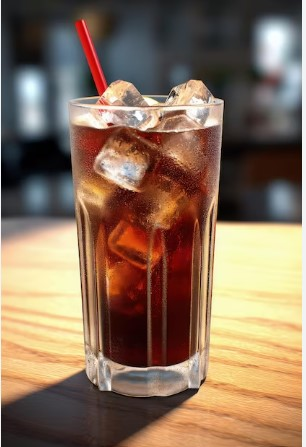
\includegraphics[scale=0.25]{figs/VN12-Y24-PH-SYL-008-1}
}
	\loigiai{Khi có cân bằng nhiệt, tổng nhiệt lượng trao đổi trong hệ bằng 0:
		$$10m_\text{đ}\lambda+m_\text{n}c_\text{n}\left(t_\text{cb}-t_0\right)=0$$
		$$\Rightarrow t_\text{cb}\approx\SI{0.69}{\celsius}.$$}
\end{ex}
% ===================================================================
\begin{ex}
	Năm 1986, một tảng băng khổng lồ đã tách ra khỏi thềm băng Ross ở Nam Cực. Tảng băng có dạng gần như hình hộp chữ nhật với chiều dài $\SI{160}{\kilo\meter}$, chiều rộng $\SI{40}{\kilo\meter}$ và dày $\SI{250}{\meter}$. Khối lượng riêng của băng là $\SI{917}{\kilogram/\meter^3}$, nhiệt nóng chảy riêng của băng là $\SI{3.34E5}{\joule/\kilogram}$. Chỉ riêng ánh sáng Mặt Trời thì phải mất bao nhiêu năm để làm tan chảy được lớp băng dày như thế \textit{(làm tròn đến 2 chữ số thập phân)}. Cho rằng công suất toả nhiệt trung bình của Mặt Trời là $\SI{100}{\watt/\meter^2}$ và Mặt Trời chiếu sáng $\SI{12}{\hour}$ mỗi ngày.
	
	\loigiai{Nhiệt lượng cần cung cấp để làm tan khối băng:
		$$Q=\rho V\lambda=Sh\rho\lambda.$$
		Nhiệt lượng do Mặt Trời cung cấp:
		$$Q=\calP t$$
		Thời gian cần để băng tan:
		$$t=\dfrac{\rho h\lambda}{\calP}=\SI{212693}{\hour}.$$
		Mỗi ngày trung bình Mặt Trời chiếu sáng $\SI{12}{\hour}$ nên nếu chỉ riêng Mặt Trời chiếu sáng thì phải mất:
		$$\dfrac{t}{12\cdot 365}\approx\SI{48.56}{\text{năm}}.$$}
\end{ex}	
%%%%%%%%%%%%%%%%%%%% OKs
\setcounter{chapter}{1}
\chapter{KHÍ LÝ TƯỞNG}
\section{MÔ HÌNH ĐỘNG HỌC PHÂN TỬ CHẤT KHÍ}
\subsection{LÝ THUYẾT TRỌNG TÂM}
\subsubsection{Chuyển động Brown}
\begin{boxdn}
	Chuyển động Brown là chuyển động hỗn loạn không ngừng, không theo quy luật, có quỹ đạo là những đường gấp khúc bất kì của các hạt nhẹ trong chất lỏng và chất khí. Chuyển động Brown chứng tỏ các phân tử chất khí chuyển động hỗn loạn, không ngừng. Nhiệt độ càng cao, các phân tử chuyển động càng nhanh.
\end{boxdn}
\begin{center}
	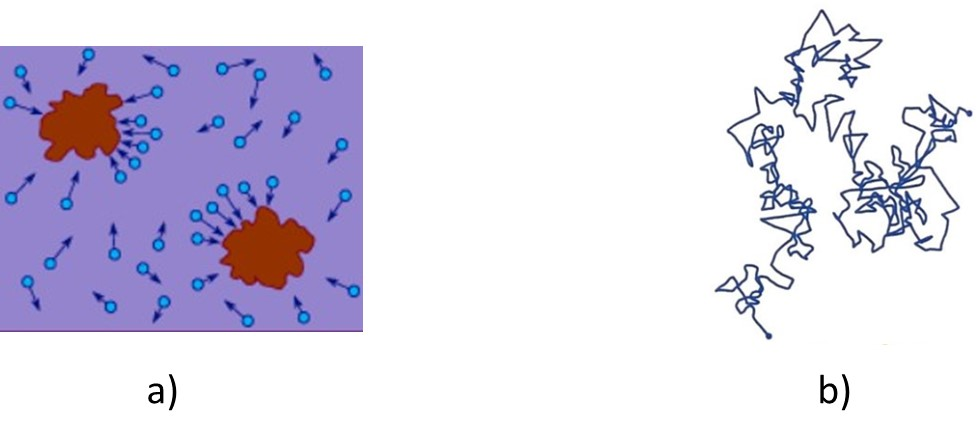
\includegraphics[width=0.5\linewidth]{figs/VN12-Y24-PH-SYL-009-1}
	\captionof{figure}{a) Va chạm của các phân tử nước lên hạt phấn hoa, b) Minh hoạ quỹ đạo gấp khúc của một hạt phấn hoa trong nước. }
\end{center}
\subsubsection{Chất khí}
\paragraph{Tính chất của chất khí}
\begin{boxdn}
	Chất khí có một số tính chất sau:
	\begin{itemize}
		\item Chất khí có hình dạng và thể tích của vật chứa nó.
		\item Chất khí có khối lượng riêng nhỏ hơn nhiều so với chất lỏng và chất rắn.
		\item Chất khí dễ bị nén.
		\item Chất khí gây ra áp suất lên thành bình chứa nó. Khi nhiệt độ tăng, áp suất khí tác dụng lên thành bình tăng.
	\end{itemize}
\end{boxdn}
\paragraph{Lượng chất}
\begin{boxdn}
	Mol là lượng chất trong đó chứa số phân tử (hoặc nguyên tử) bằng 
	$$N_A\approx\SI{6.02E23}{\mole^{-1}}$$
	$N_A$ được gọi là số Avogadro (số phân tử trong 1 mol chất).\\
	Khối lượng mol của một chất là khối lượng của $\SI{1}{\mole}$ chất đó, được kí hiệu là $M$.\\
	Nếu một mẫu chất có khối lượng $m$, chứa $N$ phân tử thì số mol $n$ của mẫu chất đó được xác định:
	$$n=\dfrac{N}{N_A}=\dfrac{m}{M}.$$
\end{boxdn}
\subsubsection{Mô hình động học phân tử chất khí}
\begin{boxdn}
	Nội dung mô hình động học phân tử chất khí gồm các ý chính như sau:
	\begin{itemize}
		\item Chất khí gồm tập hợp rất nhiều các phân tử có kích thước rất nhỏ so với khoảng cách trung bình giữa chúng.
		\item Các phân tử khí luôn chuyển động hỗn loạn, không ngừng và được gọi là chuyển động nhiệt. Nhiệt độ càng cao, các phân tử khí chuyển động càng nhanh.
		\item Trong quá trình chuyển động, các phân tử khí va chạm với thành bình chứa, gây ra áp suất lên thành bình.
	\end{itemize}
\end{boxdn}
\begin{center}
	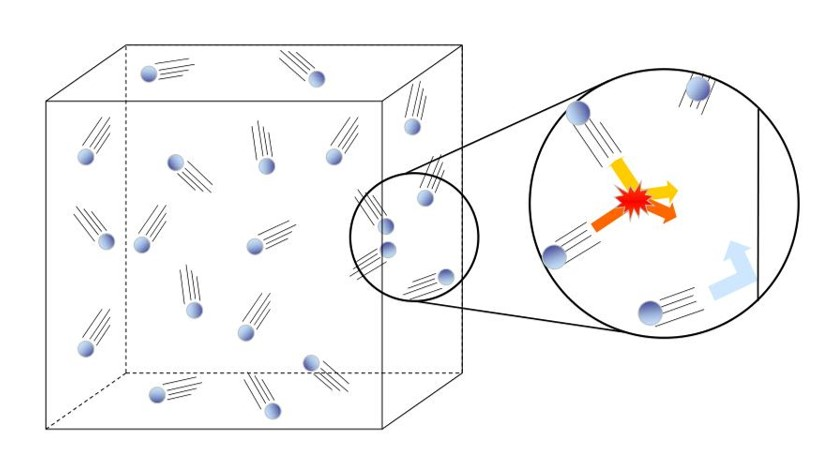
\includegraphics[width=0.4\linewidth]{figs/VN12-Y24-PH-SYL-009-2}
	\captionof{figure}{Các phân tử va chạm vào nhau và va chạm vào thành bình trong quá trình chuyển động nhiệt.}
\end{center}
\subsubsection{Khí lí tưởng}
\begin{boxdn}
	Khí lí tưởng có các đặc điểm sau:
	\begin{enumerate}[label=\arabic*.]
		\item Các phân tử khí được coi là các \textit{chất điểm}, không tương tác với nhau khi chưa va chạm.
		\item Các phân tử khí tương tác khi va chạm với nhau và va chạm với thành bình. Các va chạm này là va chạm \textit{hoàn toàn đàn hồi}.
	\end{enumerate}
\end{boxdn}
\begin{luuy}
	Mô hình khí lí tưởng đơn giản hơn khí thực (khí tồn tại trong thực tế) nhưng vẫn phản ánh được các đặc điểm cơ bản của khí này.
\end{luuy}
\subsection{VÍ DỤ MINH HOẠ}
\begin{dang}{Phân tích mô hình Brown, nêu được các phân tử trong chất khí chuyển động hỗn loạn.}
	\end{dang}
	\begin{vd}
Khi quan sát tia nắng mặt trời chiếu qua cửa sổ vào trong phòng, ta có thể thấy các hạt bụi trong ánh nắng chuyển động không ngừng. Chuyển động này có phải là chuyển động Brown không? Tại sao?
	\loigiai{Chuyển động của các hạt bụi trong trường hợp này không thể coi là chuyển động Brown vì chuyển động chủ yếu của các hạt bụi lúc bấy giờ là chuyển động theo dòng khí do hiện tượng đối lưu.
			}
	\end{vd}

\begin{dang}{Vận dụng được thuyết động học phân tử chất khí}
\end{dang}
\begin{vd}
Trong quá trình bơm xe đạp, khi lốp xe đã gần căng, càng về cuối của mỗi lần bơm thì ta càng thấy khó nén piston xuống. Hãy giải thích hiện tượng trên.
\loigiai{Càng về cuối quá trình bơm săm xe đạp, săm xe đã căng và khó tăng thể tích chứa khí bên trong. Trong khi đó, sau mỗi lần bơm thì số phân tử khí bên trong săm tăng lên đáng kể và làm tăng mật độ phân tử khí bên trong. \\
		Theo thuyết động học phân tử chất khí, khi mật độ phân tử khí bên trong săm tăng thì số va chạm của các phân tử khí lên thành săm và piston tăng. Do đó, áp suất khí tác động lên piston tăng và làm cho piston khó nén xuống hơn.
	}

\end{vd}
% ==================================================================
\begin{vd}
Một phân tử oxygen đang chuyển động qua tâm một bình cầu có đường kính $\SI{0.20}{\meter}$. Tốc độ của phân tử là $\SI{400}{\meter/\second}$. Ước tính số lần phân tử này va chạm vào thành bình chứa trong mỗi giây. Coi rằng tốc độ của phân tử là không đổi.
\loigiai{Trong điều kiện lý tưởng, xem như phân tử oxygen chuyển động thẳng và không bị đổi hướng do va chạm với các phân tử khí khác, tốc độ của phân tử là không đổi và va chạm của phân tử khí với thành bình là tuyệt đối đàn hồi. Ban đầu phân tử khí này chuyển động qua tâm bình cầu nên khi chạm vào thành bình, phân tử khí sẽ bật ngược trở lại với tốc độ như cũ và cũng đi qua tâm bình cầu.\\
		Khoảng thời gian giữa 2 lần liên tiếp phân tử khí va chạm với thành bình:
		$$T=\dfrac{2R}{v}=\dfrac{\SI{0.2}{\meter}}{\SI{400}{\meter/\second}}=\SI{5E-4}{\second}.$$
		Số lần phân tử khí này va chạm vào thành bình trong mỗi giây:
		$$f=\dfrac{1}{T}=2000.$$
	}
\end{vd}
\subsection{BÀI TẬP TRẮC NGHIỆM}
\Opensolutionfile{ans}[ans/G12Y24B8TN]
% ===================================================================
\begin{ex}
	Tính chất nào sau đây \textbf{không phải} là tính chất của chất khí?
	\choice
	{\True Có hình dạng và thể tích riêng.}
	{Có các phân tử chuyển động hỗn loạn không ngừng.}
	{Có thể nén được dễ dàng.}
	{Có khối lượng riêng nhỏ hơn so với chất rắn và chất lỏng.}
	\loigiai{}
\end{ex}
% ===================================================================
\begin{ex}
	Chọn phương án \textbf{sai}. Số Avogadro là
	\choice
	{số phân tử (hay nguyên tử) có trong $\SI{22.4}{\text{lít}}$ khí ở điều kiện tiêu chuẩn $\left(\SI{0}{\celsius}, \SI{1}{atm}\right)$.}
	{số phân tử (hay nguyên tử) có trong 1 mol chất.}
	{\True số phân tử (hay nguyên tử) có trong 1 đơn vị khối lượng chất.}
	{số nguyên tử có trong $\SI{12}{\gram}$ $\ce{^{12}C}$.}
	\loigiai{}
\end{ex}
% ===================================================================
\begin{ex}
Gọi $\xsi{M}{(\gram/\mole)}$ là khối lượng mol nguyên tử, $N_\text{A}$ là số Avogadro. Biểu thức xác định số phân tử hay nguyên tử chứa trong $\xsi{m}{(\gram)}$ của chất đó là	
	\choice
	{$N=MmN_\text{A}$.}
	{$N=\dfrac{MN_\text{A}}{m}$.}
	{\True $N=\dfrac{mN_\text{A}}{M}$.}
	{$N=\dfrac{N_\text{A}}{mM}$.}
	\loigiai{}
\end{ex}
% ===================================================================
\begin{ex}
Điền vào chỗ trống.\\
Chất khí trong đó các phân tử được coi là \dots và chỉ tương tác khi \dots được gọi là khí lí tưởng.	
	\choice
	{\True chất điểm; va chạm.}
	{vật rắn; va chạm.}
	{chất điểm; ở gần nhau.}
	{vật rắn; ở gần nhau.}
	\loigiai{}
\end{ex}
% ===================================================================
\begin{ex}
	Nhận xét nào sau đây về các phân tử khí lí tưởng là \textbf{không đúng}?
	\choice
	{Có thể tích riêng không đáng kể.}
	{Có lực tương tác không đáng kể khi không va chạm.}
	{\True Có khối lượng không đáng kể.}
	{Có vận tốc càng lớn khi nhiệt độ phân tử càng cao.}
	\loigiai{}
\end{ex}
% ===================================================================
\begin{ex}
Chọn câu \textbf{sai}. Số Avogadro có giá trị bằng	
	\choice
	{số nguyên tử chứa trong $\SI{4}{\gram}$ helium.}
	{\True số phân tử chứa trong $\SI{16}{\gram}$ oxygen.}
	{số phân tử chứa trong $\SI{18}{\gram}$ nước lỏng.}
	{số nguyên tử chứa trong $\SI{22.4}{\liter}$ khí trơ ở $\SI{0}{\celsius}$ và áp suất $\SI{1}{atm}$.}
	\loigiai{}
\end{ex}
% ===================================================================
\begin{ex}
Một bình kín chứa $N=\SI{3.01E23}{}$ phân tử khí helium. Khối lượng helium chứa trong bình là	
	\choice
	{$\SI{0.5}{\gram}$.}
	{$\SI{1}{\gram}$.}
	{\True $\SI{2}{\gram}$.}
	{$\SI{4}{\gram}$.}
	\loigiai{}
\end{ex}
% ===================================================================
\begin{ex}
	Cho biết khối lượng riêng của không khí ở điều kiện tiêu chuẩn là $\SI{1.29}{\kilogram/\meter^3}$. Coi không khí như một chất khí thuần nhất, khối lượng mol của không khí là
	\choice
	{$\SI{0.041}{\kilogram/\mole}$.}
	{\True $\SI{0.029}{\kilogram/\mole}$.}
	{$\SI{0.023}{\kilogram/\mole}$.}
	{$\SI{0.026}{\kilogram/\mole}$.}
	\loigiai{$$\rho=\dfrac{m}{V}=\dfrac{m}{n\cdot\left(\SI{22.4E-3}{\meter^3}\right)}\Rightarrow M=\dfrac{m}{n}=\SI{0.029}{\kilogram/\mole}.$$}
\end{ex}
\Closesolutionfile{ans}
\subsection{TRẮC NGHIỆM ĐÚNG/SAI}
\setcounter{ex}{0}
% ===================================================================
\begin{ex}
	Nhận định các phát biểu sau về đặc điểm của chuyển động Brown.
	\begin{enumerate}[label=\alph*)]
	\item Chuyển động Brown tuân theo một số quy luật nhất định.
	\item Quỹ đạo của chuyển động Brown là những đường gấp khúc.
	\item Chuyển động Brown là chuyển động của các hạt nhẹ trong chất rắn, lỏng, khí.
	\item Nhiệt độ càng cao thì các phân tử khí chuyển động càng hỗn loạn.
\end{enumerate}
	\loigiai{\begin{enumerate}[label=\alph*)]
			\item Sai. Chuyển động Brown không theo quy luật.
			\item Đúng.
			\item Sai. Chuyển động Brown là chuyển động của các hạt nhẹ trong chất lỏng và chất khí.
			\item Đúng.
		\end{enumerate}
	}
\end{ex}
% ===================================================================
\begin{ex}
	Nhận định các phát biểu sau về nội dung thuyết động học phân tử chất khí.
	\begin{enumerate}[label=\alph*)]
		\item Chất khí gồm tập hợp nhiều các phân tử dao động nhiệt quanh các vị trí cân bằng của chúng.
		\item Nhiệt độ càng cao thì các phân tử khí chuyển động nhiệt càng nhanh.
		\item Kích thước các phân tử rất nhỏ so với khoảng cách trung bình giữa chúng.
		\item Áp suất khí được tạo ra bởi sự va chạm giữa các phân tử khí với nhau.
	\end{enumerate}
	\loigiai{\begin{enumerate}[label=\alph*)]
			\item Sai. Các phân tử khí chuyển động hỗn loạn, không ngừng.
			\item Đúng.
			\item Đúng.
			\item Sai. Sự va chạm của các phân tử khí với thành bình gây ra áp suất lên thành bình.
		\end{enumerate}
	}
\end{ex}
% ===================================================================
\begin{ex}
	Nhận định các phát biểu sau đây về đặc điểm của khí lí tưởng
	\begin{enumerate}[label=\alph*)]
		\item Các phân tử khí được coi là chất điểm nên người ta có thể bỏ qua khối lượng các phân tử khí.
		\item Thể tích khối khí bằng thể tích bình chứa trừ đi thể tích riêng của các phân tử.
		\item Các phân tử khí chỉ tương tác với nhau khi va chạm.
		\item Nội năng của khối khí bằng tổng động năng chuyển động nhiệt của các phân tử khí và chỉ phụ thuộc vào nhiệt độ.
	\end{enumerate}
	
	\loigiai{\begin{enumerate}[label=\alph*)]
			\item Sai. Các phân tử khí được coi là chất điểm nên người ta có thể bỏ qua kích thước các phân tử khí.
			\item Sai. Thể tích khối khí bằng thể tích bình chứa.
			\item Đúng.
			\item Đúng.
		\end{enumerate}
	}
\end{ex}
% ===================================================================
\begin{ex}
	Một người xịt nước hoa ở đầu phòng thì người ở cuối phòng vẫn nghe được mùi hương của nước hoa.
	\begin{enumerate}[label=\alph*)]
		\item Hiện tượng trên được gọi là sự khuếch tán.
		\item Các phân tử nước hoa chuyển động thành dòng từ đầu phòng sang cuối phòng chỉ nhờ vào đối lưu.
		\item Hiện tượng trên chứng tỏ nhiệt độ ở đầu phòng cao hơn nhiệt độ ở cuối phòng.
		\item Nhiệt độ trong phòng càng cao thì người ở cuối phòng càng sớm nhận ra mùi nước hoa.
	\end{enumerate}
	
	\loigiai{\begin{enumerate}[label=\alph*)]
			\item Đúng.
			\item Sai. Sự dao động nhiệt của các phân tử khí và phân tử nước hoa làm cho chúng khuếch tán vào nhau.
			\item Sai. Các phân tử khí chuyển động hỗn loạn, không ngừng về mọi phía nên không thể khẳng định được nhiệt độ nơi nào cao hơn.
			\item Đúng. Nhiệt độ càng cao, các phân tử chuyển động càng nhanh làm tốc độ khuếch tán diễn ra càng nhanh.
		\end{enumerate}
	}
\end{ex}
\subsection{BÀI TẬP TỰ LUẬN}
\setcounter{ex}{0}
% ===================================================================
\begin{ex}
	Mùi hôi từ các bãi rác thải là một vấn nạn đối với cư dân sống xung quanh. Khi thời tiết càng nắng nóng thì mùi hôi bốc ra càng nồng nặc và càng bay xa (ngay cả trong điều kiện không có gió). Dựa vào thuyết động học phân tử chất khí, hãy giải thích điều này và đề xuất biện pháp hạn chế tình trạng trên.
	\loigiai{Thời tiết càng nóng thì quá trình phân huỷ các chất hữu cơ diễn ra càng nhanh và sinh ra nhiều khí có mùi hôi như: $\ce{H_2S}, \ce{NH_3}, \ce{CH_4}, \ce{SO_2},\dots$. Bên cạnh đó, nhiệt độ càng cao thì các phân tử khí chuyển động nhiệt càng nhanh, do đó các phân tử khí này càng dễ khuếch tán vào không khí và bay đi xa hơn.\\
		Biện pháp hạn chế: Thường xuyên thu gom, xử lý rác thải, nâng cao ý thức cộng đồng.
	}
\end{ex}
% ===================================================================
\begin{ex}
Đun một nồi nước trên bếp, khi nước sôi nắp nồi thường bị đẩy lên. Hãy giải thích điều này.
	
	\loigiai{Khi đun nước đến nhiệt độ sôi, nước sẽ bay hơi tạo thành hơi nước. Bên cạnh đó, nhiệt độ càng cao làm cho các phân tử khí và hơi nước trong nồi chuyển động càng nhanh. Sự gia tăng mật độ khí và tốc độ chuyển động nhiệt của các phân tử khí và hơi nước trong nồi làm gia tăng số lượt va chạm của các phân tử khí lên nắp nồi $\rightarrow$ tăng áp suất khí tác dụng lên nắp và làm nắp bị đẩy lên.
	}
\end{ex}
% ===================================================================
\begin{ex}
	Xác định số phân tử chứa trong
	\begin{enumerate}[label=\alph*)]
		\item $\SI{0.2}{\kilogram}$ nước.
		\item $\SI{1}{\kilogram}$ không khí nếu như không khí có $\SI{22}{\percent}$ là khí $\ce{O_2}$ và $\SI{78}{\percent}$ là khí $\ce{N_2}$.
	\end{enumerate}
	\loigiai{\begin{enumerate}[label=\alph*)]
			\item $N=\dfrac{m}{M_{\ce{H_2O}}}\cdot N_\text{A}\approx\SI{6.68E24}{\text{phân tử}}.$
			\item $N=\SI{22}{\percent}\cdot\dfrac{m}{M_{\ce{O_2}}}\cdot N_\text{A}+\SI{78}{\percent}\cdot\dfrac{m}{M_{\ce{N_2}}}\cdot N_\text{A}\approx\SI{2.1E25}{\text{phân tử}}.$
		\end{enumerate}
	}
\end{ex}
% ===================================================================
\begin{ex}
	Coi Trái Đất là một khối cầu bán kính $\SI{6400}{\kilo\meter}$, nếu lấy toàn bộ số phân tử nước trong $\SI{1.0}{\gram}$ hơi nước trải đều trên bề mặt Trái Đất thì mỗi mét vuông trên bề mặt Trái Đất có bao nhiêu phân tử nước? Biết khối lượng mol của phân tử nước khoảng $\SI{18}{\gram/\mole}$.
	\loigiai{$$\eta=\dfrac{N}{S}=\dfrac{\dfrac{m}{M}N_\text{A}}{4\pi R^2}=\SI{64.98E6}{\text{phân tử}/\meter^2}.$$}
\end{ex}	
\newpage\section{ĐỊNH LUẬT BOYLE}
\subsection{LÝ THUYẾT TRỌNG TÂM}
\subsubsection{Trạng thái và quá trình biến đổi trạng thái}
\begin{boxdn}
	\textbf{Trạng thái của một khối khí } được xác định bằng ba thông số, gọi là thông số trạng thái của khối khí: thể tích $V$, áp suất $p$ và nhiệt độ tuyệt đối $T$. Giữa các thông số trạng thái của một khối khí xác định có những mối liên hệ mang tính quy luật.
\end{boxdn}
\begin{center}
	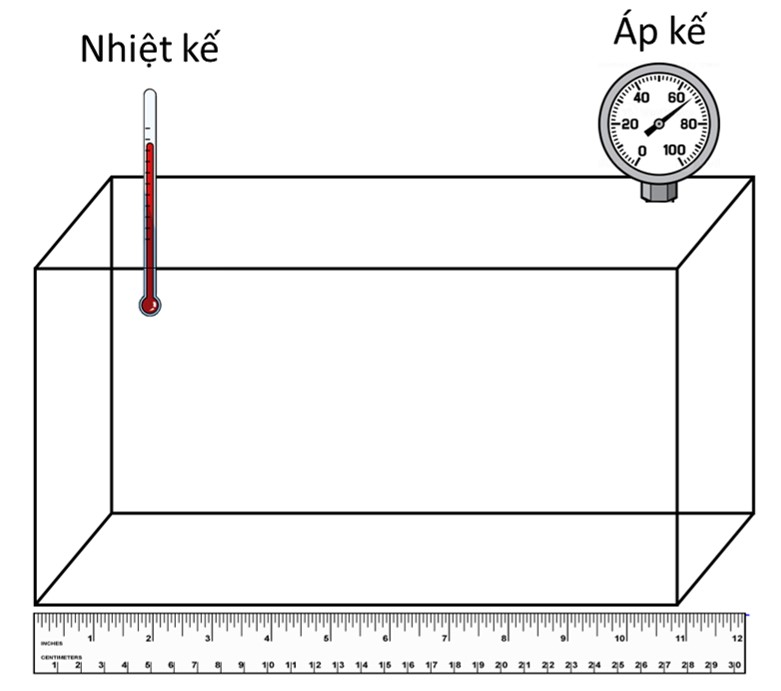
\includegraphics[width=0.35\linewidth]{figs/VN12-Y24-PH-SYL-010-1}
	\captionof{figure}{Xác định các thông số trạng thái của một lượng khí}
\end{center}
\begin{boxdn}
	\textbf{Quá trình biến đổi trạng thái là} quá trình khối khí biến đổi từ trạng thái này sang trạng thái khác.\\
	\textbf{Đẳng quá trình} là quá trình biến đổi trạng thái mà trong đó có một thông số trạng thái được giữ không đổi.\\
	Các đẳng quá trình:
	\begin{itemize}
		\item Đẳng nhiệt là quá trình biến đổi trạng thái của một khối khí xác định, trong đó nhiệt độ được giữ không đổi.
		\item Đẳng áp là quá trình biến đổi trạng thái của một khối khí xác định, trong đó áp suất được giữ không đổi.
		\item Đẳng tích là quá trình biến đổi trạng thái của một khối khí xác định, trong đó thể tích được giữ không đổi.
	\end{itemize}
\end{boxdn}
\begin{luuy}
	Vì chất khí luôn chiếm toàn bộ dung tích của bình chứa nên thể tích của một lượng khí bằng dung tích bình chứa nó.
\end{luuy}
\subsubsection{Định luật Boyle}
\begin{boxdl}
	Ở nhiệt độ không đổi, áp suất của một khối khí xác định tỉ lệ nghịch với thể tích của nó.
	\begin{equation}
		pV=\text{hằng số}
	\end{equation}
\end{boxdl}
Đường biểu diễn sự phụ thuộc của $p$ theo $V$ khi nhiệt độ của khối khí không đổi gọi là \textbf{đường đẳng nhiệt}.
\begin{center}
	\begin{tikzpicture}  
		\begin{axis}[  ultra thick,
			xmin=0,  
			xmax=24,  
			xtick=\empty,
			ytick=\empty,
			ymin=0,  
			ymax=5.8, 
			samples=300,
			xticklabels=\empty,
			yticklabels=\empty,
			axis lines=center, 
			xlabel=$V$, 
			ylabel=$p$, 
			every axis y label/.style={at=(current axis.above origin),anchor=south},  
			every axis x label/.style={at=(current axis.right of origin),anchor=west},  ]
			\addplot [ultra thick, blue, smooth, domain=1:20] {5/x} node[right] {$T_1$}; 
			\addplot [ultra thick, red, smooth, domain=3:20] {15/x} node[right] {$T_2$}; 
		\end{axis}  
		\node[label={[below left]90:O}] at (0,0){};
	\end{tikzpicture}
	\captionof{figure}{Các đường đẳng nhiệt của một khối khí lí tưởng tương ứng với nhiệt độ $T_1$ và $T_2\left(T_2>T_1\right)$}
	
\end{center}
\subsection{Mục tiêu bài học - Ví dụ minh hoạ}
\begin{dang}{Vận dụng định luật Boyle giải thích được một số hiện tượng trong thực tế}
	\end{dang}
\begin{vd}
Nếu lật úp một chiếc cốc thuỷ tinh rồi nhúng chìm chiếc cốc vào trong nước thì thể tích phần không khí bị giam trong cốc sẽ thay đổi như thế nào trong quá trình chiếc cốc chìm sâu xuống nước?
\loigiai{
			Trong quá trình cốc chìm xuống nước thì nhiệt độ không khí trong cốc không thay đổi. Cốc càng chìm sâu vào trong nước thì áp suất của không khí trong cốc càng tăng. Theo định luật Boyle, khi đó thể tích của không khí bị giam trong cốc ngày càng giảm.
}
\end{vd}
% ======================================================
\begin{vd}
Để đưa thuốc từ lọ vào trong cylanh của ống tiêm, ban đầu nhân viên y tế đẩy piston sát đáy cylanh, sau đó đưa đầu kim tiêm (được gắn với ống tiêm) vào trong lọ thuốc. Khi kéo piston, thuốc sẽ chảy vào trong cylanh. Em hãy giải thích cơ sở khoa học của việc làm trên?
	\begin{center}
		
\includegraphics[width=0.35\linewidth]{figs/VN12-Y24-PH-SYL-010-2}
	\end{center}
\loigiai{
		Khi mới đưa đầu kim tiêm vào trong lọ thuốc, áp suất khí còn lại trong cylanh bằng áp suất chất lỏng trong lo thuốc. Khi kéo piston, thể tích khí trong cylanh tăng (nhiệt độ khí gần như không đổi). Theo định luật Boyle, áp suất khí trong cylanh giảm và nhỏ hơn áp suất chất lỏng trong lọ. Do đó, chất lỏng trong lọ bị đẩy qua kim và chảy sang cylanh cho đến khi có sự cân bằng áp suất ở cả hai phía.
	}
\end{vd}

\begin{dang}{Giải được các bài toán liên quan quá trình đẳng nhiệt}
\end{dang}
\begin{vd}
Một lượng khí có thể tích $\SI{10}{\text{lít}}$ ở áp suất $\SI{E5}{\pascal}$. Tính thể tích của lượng khí này ở áp suất $\SI{1.25E5}{\pascal}$. Biết nhiệt độ của khí không đổi.
\loigiai{
		\begin{center}
			\begin{tabular}{C{4cm} C{3cm} C{4cm}}
				\colorbox{yellow}{\textcolor{red}{\textbf{Trạng thái 1}}} & $\xrightarrow[]{T_1=T_2}$ & \colorbox{yellow}{\textcolor{red}{\textbf{Trạng thái 2}}}\\
				$p_1=\SI{E5}{\pascal}$ & &$p_2=\SI{1.25E5}{\pascal}$\\
				$V_1=\SI{10}{\text{lít}}$ & & $V_2=?$
			\end{tabular}
		\end{center}
		Theo định luật Boyle:
		$$p_1V_1=p_2V_2\Rightarrow V_2=\dfrac{p_1V_1}{p_2}=\dfrac{\left(\SI{E5}{\pascal}\right)\cdot\left(\SI{10}{\text{lít}}\right)}{\SI{1.25E5}{\pascal}}=\SI{8}{\text{lít}}.$$
		Vậy: ở áp suất $\SI{1.25E5}{\pascal}$ thì thể tích bọt khí là $\SI{8}{\text{lít}}$.
}
\end{vd}
% ===============================================================	
\begin{vd}
Một bọt khí nổi lên từ đáy giếng sâu $\SI{6}{\meter}$ lên mặt nước. Khi lên tới mặt nước, thể tích của bọt khí tăng lên bao nhiêu lần? Coi áp suất khí quyển là $\SI{1.013E5}{\pascal}$; khối lượng riêng của nước giếng là $\SI{1003}{\kilogram/\meter^3}$ và nhiệt độ của nước giếng không thay đổi theo độ sâu. Lấy gia tốc trọng trường $g=\SI{9.81}{\meter/\second^2}$.
\loigiai{
		Áp suất trong bọt khí khi ở độ sâu $\SI{6}{\meter}$ so với mặt nước:
		$$p_1=p_0+\rho gh=\SI{1.013E5}{\pascal}+\left(\SI{1003}{\kilogram/\meter^3}\right)\cdot\left(\SI{9.81}{\meter
			/\second^2}\right)\cdot\left(\SI{6}{\meter}\right)\approx\SI{1.6E5}{\pascal}$$
		\begin{center}
			\begin{tabular}{C{4cm} C{3cm} C{4cm}}
				\colorbox{yellow}{\textcolor{red}{\textbf{Trạng thái 1}}} & $\xrightarrow[]{T_1=T_2}$ & \colorbox{yellow}{\textcolor{red}{\textbf{Trạng thái 2}}}\\
				$p_1=\SI{1.6E5}{\pascal}$ & &$p_2=p_0=\SI{1.013E5}{\pascal}$\\
				$V_1$ & & $V_2$
			\end{tabular}
		\end{center}
		Theo định luật Boyle:
		$$p_1V_1=p_2V_2\Rightarrow \dfrac{V_2}{V_1}=\dfrac{p_1}{p_2}=\dfrac{\SI{1.6E5}{\pascal}}{\SI{1.013E5}{\pascal}}\approx1,58.$$
		Vậy: khi nổi lên mặt nước, thể tích bọt khí đã tăng lên 1,58 lần.
}
\end{vd}
% ==============================================================
\begin{vd}
	Một cột không khí chứa trong một ống nhỏ, dài, tiết diện đều, ban đầu ống được đặt nằm ngang (như hình). Cột không khí được ngăn cách bởi một cột thuỷ ngân có chiều dài $d=\SI{150}{\milli\meter}$. Áp suất khí quyển là $p_0=\SI{750}{\milli\meter Hg}$. Biết chiều dài ban đầu của cột không khí là $\ell_0=\SI{144}{\milli\meter}$.
		\begin{center}
			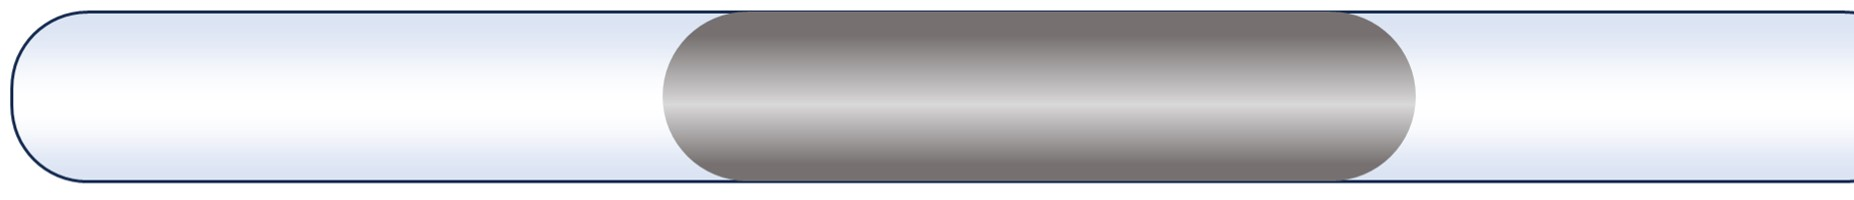
\includegraphics[width=0.4\linewidth]{figs/VN12-Y24-PH-SYL-010-3}
		\end{center}
		Hãy tính chiều dài cột không khí nếu:
		\begin{enumerate}[label=\alph*)]
			\item ống thẳng đứng, miệng ống ở trên.
			\item ống thẳng đứng, miệng ống ở dưới.
			\item ống đặt nghiêng góc $\alpha=\SI{30}{\degree}$ so với phương ngang, miệng ống ở dưới.
			\item ống đặt nghiêng góc $\alpha=\SI{30}{\degree}$ so với phương ngang, miệng ống ở trên.
		\end{enumerate}
		Giả sử ống đủ dài để cột thuỷ ngân luôn ở trong ống và nhiệt độ là không đổi.
	\loigiai{Gọi $S$ là tiết diện của ống.
			\begin{enumerate}[label=\alph*)]
				\item Trường hợp ống đặt thẳng đứng, miệng ống hướng lên:\\
				\begin{minipage}[l]{0.25\textwidth}
					\begin{center}
						
\includegraphics[width=0.1\linewidth]{figs/VN12-Y24-PH-SYL-010-4}
					\end{center}
				\end{minipage}
				\begin{minipage}[l]{0.75\textwidth}
					\begin{center}
						\begin{tabular}{C{4cm} C{2cm} C{4cm}}
							\colorbox{yellow}{\textcolor{red}{\textbf{Trạng thái ban đầu}}} & $\xrightarrow[]{T=const}$ & \colorbox{yellow}{\textcolor{red}{\textbf{Trạng thái câu a}}}\\
							$p_0=\SI{750}{\milli\meter Hg}$ & &$p_a=p_0+d=\SI{900}{\milli\meter Hg}$\\
							$V_0=\ell_0S$ & & $V_a=\ell_a S$
						\end{tabular}
					\end{center}
					Theo định luật Boyle:
					$$p_0V_0=p_aV_a$$
					$$\Leftrightarrow p_0\ell_0S=p_a\ell_aS$$
					$$\Rightarrow \ell_a=\dfrac{p_0\ell_0}{p_a}=\dfrac{\left(\SI{750}{\milli\meter Hg}\right)\cdot\left(\SI{144}{\milli\meter}\right)}{\SI{900}{\milli\meter Hg}}=\SI{120}{\milli\meter}.$$
				\end{minipage}
				\item Trường hợp ống đặt thẳng đứng, miệng ống hướng xuống:\\
				\begin{minipage}[l]{0.25\textwidth}
					\begin{center}
						
\includegraphics[width=0.1\linewidth]{figs/VN12-Y24-PH-SYL-010-5}
					\end{center}
				\end{minipage}
				\begin{minipage}[l]{0.75\textwidth}
					\begin{center}
						\begin{tabular}{C{4cm} C{2cm} C{4cm}}
							\colorbox{yellow}{\textcolor{red}{\textbf{Trạng thái ban đầu}}} & $\xrightarrow[]{T=const}$ & \colorbox{yellow}{\textcolor{red}{\textbf{Trạng thái câu b}}}\\
							$p_0=\SI{750}{\milli\meter Hg}$ & &$p_b=p_0-d=\SI{600}{\milli\meter Hg}$\\
							$V_0=\ell_0S$ & & $V_b=\ell_b S$
						\end{tabular}
					\end{center}
					Theo định luật Boyle:
					$$p_0V_0=p_bV_b$$
					$$\Leftrightarrow p_0\ell_0S=p_b\ell_bS$$
					$$\Rightarrow \ell_b=\dfrac{p_0\ell_0}{p_b}=\dfrac{\left(\SI{750}{\milli\meter Hg}\right)\cdot\left(\SI{144}{\milli\meter}\right)}{\SI{600}{\milli\meter Hg}}=\SI{180}{\milli\meter}.$$
				\end{minipage}
				\item Trường hợp ống đặt nghiêng góc $\alpha=\SI{30}{\degree}$ so với phương ngang, miệng ống ở dưới:\\
				\begin{minipage}[l]{0.25\textwidth}
					\begin{center}
						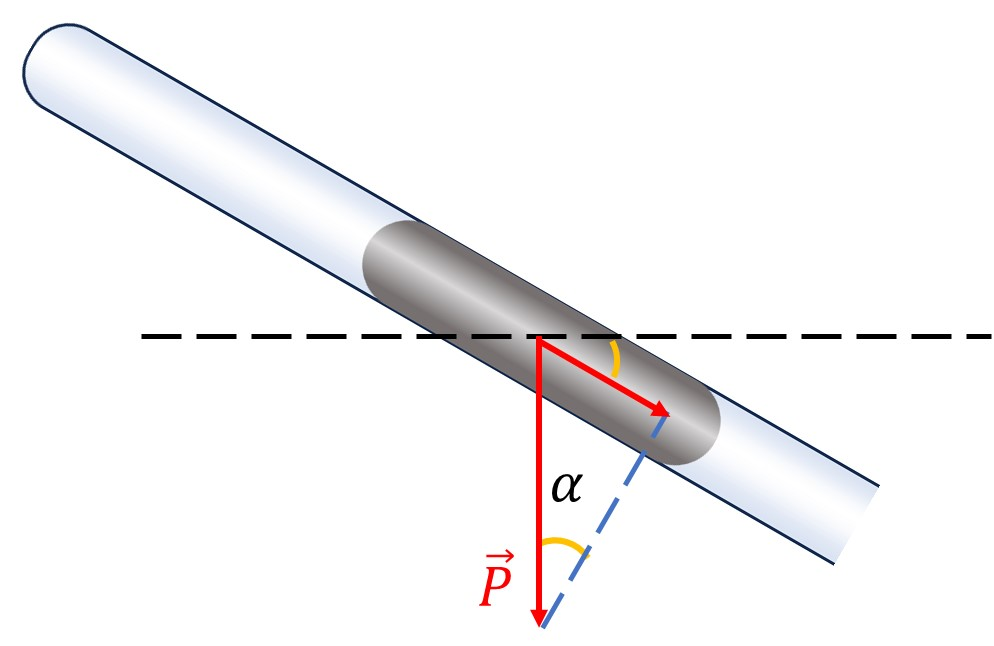
\includegraphics[width=1.0\linewidth]{figs/VN12-Y24-PH-SYL-010-6}
					\end{center}
				\end{minipage}
				\begin{minipage}[l]{0.75\textwidth}
					\begin{center}
						\begin{tabular}{C{4cm} C{1.5cm} C{4.5cm}}
							\colorbox{yellow}{\textcolor{red}{\textbf{Trạng thái ban đầu}}} & $\xrightarrow[]{T=const}$ & \colorbox{yellow}{\textcolor{red}{\textbf{Trạng thái câu c}}}\\
							$p_0=\SI{750}{\milli\meter Hg}$ & &$p_c=p_0-d\sin\alpha=\SI{675}{\milli\meter Hg}$\\
							$V_0=\ell_0S$ & & $V_c=\ell_c S$
						\end{tabular}
					\end{center}
					Theo định luật Boyle:
					$$p_0V_0=p_cV_c$$
					$$\Leftrightarrow p_0\ell_0S=p_c\ell_cS$$
					$$\Rightarrow \ell_c=\dfrac{p_0\ell_0}{p_c}=\dfrac{\left(\SI{750}{\milli\meter Hg}\right)\cdot\left(\SI{144}{\milli\meter}\right)}{\SI{675}{\milli\meter Hg}}=\SI{160}{\milli\meter}.$$
				\end{minipage}
				\item Trường hợp ống đặt nghiêng góc $\alpha=\SI{30}{\degree}$ so với phương ngang, miệng ống ở trên:\\
				\begin{minipage}[l]{0.25\textwidth}
					\begin{center}
						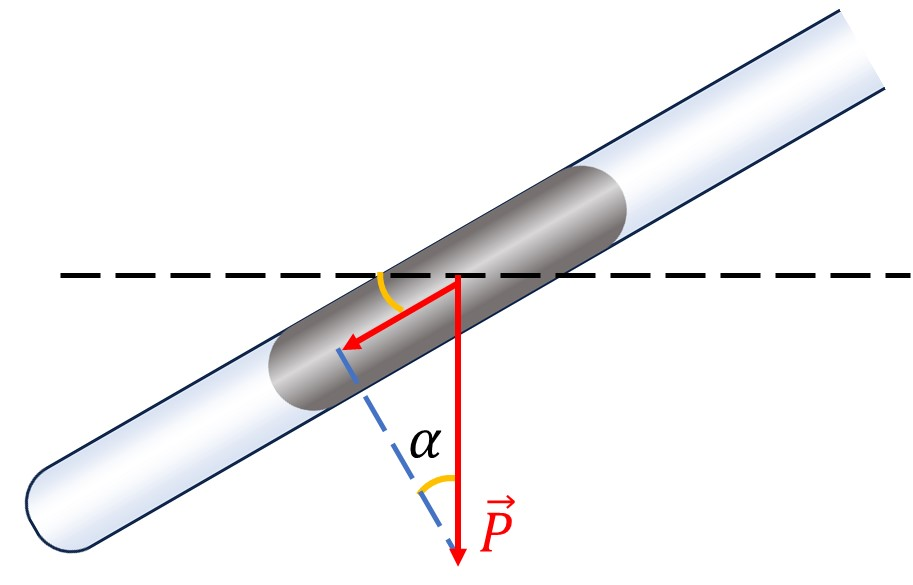
\includegraphics[width=1.0\linewidth]{figs/VN12-Y24-PH-SYL-010-7}
					\end{center}
				\end{minipage}
				\begin{minipage}[l]{0.75\textwidth}
					\begin{center}
						\begin{tabular}{C{4cm} C{1.5cm} C{4.5cm}}
							\colorbox{yellow}{\textcolor{red}{\textbf{Trạng thái ban đầu}}} & $\xrightarrow[]{T=const}$ & \colorbox{yellow}{\textcolor{red}{\textbf{Trạng thái câu d}}}\\
							$p_0=\SI{750}{\milli\meter Hg}$ & &$p_d=p_0+d\sin\alpha=\SI{825}{\milli\meter Hg}$\\
							$V_0=\ell_0S$ & & $V_d=\ell_d S$
						\end{tabular}
					\end{center}
					Theo định luật Boyle:
					$$p_0V_0=p_dV_d$$
					$$\Leftrightarrow p_0\ell_0S=p_d\ell_dS$$
					$$\Rightarrow \ell_d=\dfrac{p_0\ell_0}{p_d}=\dfrac{\left(\SI{750}{\milli\meter Hg}\right)\cdot\left(\SI{144}{\milli\meter}\right)}{\SI{825}{\milli\meter Hg}}\approx\SI{131}{\milli\meter}.$$
				\end{minipage}
			\end{enumerate}
	}
\end{vd}
\begin{dang}{Giải được bài toán piston cân bằng}
	\end{dang}
\begin{vd}
	Một lượng không khí có thể tích $\SI{240}{\centi\meter^3}$ chứa trong một cylanh có piston đóng kín, tiết diện của piston là $\SI{24}{\centi\meter^2}$. Áp suất của không khí trong cylanh bằng áp suất không khí bên ngoài là $\SI{E5}{\pascal}$. Cần một lực tối thiểu bằng bao nhiêu để dịch chuyển piston một đoạn $\SI{2}{\centi\meter}$ theo chiều làm thể tích khí giảm? Bỏ qua ma sát giữa giữa piston và thành cylanh. Coi trong quá trình piston chuyển động thì nhiệt độ của không khí không thay đổi.
	\begin{center}
		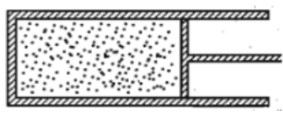
\includegraphics[width=0.25\linewidth]{figs/VN12-Y24-PH-SYL-010-8}
	\end{center}
\loigiai{
	\begin{center}
		\begin{tabular}{C{6cm} C{2cm} C{7cm}}
			\colorbox{yellow}{\textcolor{red}{\textbf{Trạng thái 1}}} & $\xrightarrow[]{T_1=T_2}$ & \colorbox{yellow}{\textcolor{red}{\textbf{Trạng thái 2}}}\\
			$p_1=\SI{E5}{\pascal}$ & &$p_2=?$\\
			$V_1=\SI{240}{\centi\meter^3}$ & & $V_2=\SI{240}{\centi\meter^3}-\left(\SI{24}{\centi\meter^2}\right)\cdot\left(\SI{2}{\centi\meter}\right)=\SI{192}{\centi\meter^3}$
		\end{tabular}
	\end{center}
	Theo định luật Boyle:
	$$p_1V_1=p_2V_2\Rightarrow p_2=\dfrac{p_1V_1}{V_2}=\dfrac{\left(\SI{100}{\kilo\pascal}\right)\cdot\left(\SI{240}{\centi\meter^3}\right)}{\SI{192}{\centi\meter^3}}=\SI{125}{\kilo\pascal}.$$
	\begin{center}
		\includegraphics[width=0.25\linewidth]{figs/VN12-Y24-PH-SYL-010-9}
	\end{center}
	Piston cân bằng khi:
	$$p_2S=p_0S+F\Rightarrow F=\left(p_2-p_0\right)S=\left(\SI{125E3}{\pascal}-\SI{100E3}{\pascal}\right)\cdot\left(\SI{24E-4}{\meter^2}\right)=\SI{60}{\newton}.$$
}
\end{vd}
% ===============================================================
\begin{vd}
	Một bình hình trụ kín hai đầu có độ cao $h=\SI{40}{\centi\meter}$, được đặt nằm ngang, bên trong có một piston rất mỏng và có thể dịch chuyển không ma sát trong bình. Lúc đầu piston được giữ cố định ở chính giữa bình. Hai bên piston chứa cùng loại khí nhưng áp suất khí bên trái $\left(p_1\right)$ lớn gấp 3 lần áp suất khí chứa ở bên phải $\left(p_2\right)$. Piston và thành bình đều được làm từ vật liệu cách nhiệt. Khi thả để piston di chuyển tự do thì piston sẽ di chuyển một đoạn bao nhiêu, theo chiều nào?
		\begin{center}
			\includegraphics[width=0.25\linewidth]{figs/VN12-Y24-PH-SYL-010-10}
		\end{center}
\loigiai{
			Vì áp suất khí bên trái lớn hơn áp suất khí bên phải nên khi được thả tự do piston sẽ di chuyển theo chiều từ trái sang phải.\\
			Piston di chuyển đến khi áp suất khí hai bên piston cân bằng. Gọi:
			\begin{itemize}
				\item $p$ là áp suất khí mỗi bên khi piston đạt trạng thái cân bằng;
				\item $x$ là độ dời của piston.
			\end{itemize}
			Áp dụng định luật Boyle cho khí ở mỗi vách ngăn khi vừa thả piston và khi piston cân bằng:
			$$pV=\text{const}\Rightarrow \begin{cases}
				p_1\cdot\dfrac{hS}{2}=p\left(\dfrac{h}{2}+x\right)S\\
				p_2\cdot\dfrac{hS}{2}=p\left(\dfrac{h}{2}-x\right)S\\
			\end{cases}\Rightarrow \dfrac{p_1}{p_2}=\dfrac{\SI{20}{\centi\meter}+x}{\SI{20}{\centi\meter}-x}=3\Rightarrow x=\SI{10}{\centi\meter}.$$
			
	}
\end{vd}
\subsection{BÀI TẬP TRẮC NGHIỆM}
\Opensolutionfile{ans}[ans/G12Y24B9TN]
% ===================================================================
\begin{ex}
	Tập hợp ba thông số xác định trạng thái của một lượng khí xác định là
	\choice
	{áp suất, thể tích, khối lượng}
	{\True áp suất, nhiệt độ, thể tích}
	{thể tích, trọng lượng, áp suất}
	{áp suất, nhiệt độ, số mol}
	\loigiai{}
\end{ex}
% ===================================================================
\begin{ex}
	Quá trình đẳng nhiệt là
	
	\choice
	{quá trình biến đổi trạng thái của một lượng khí xác định trong đó áp suất được giữ không đổi}
	{quá trình biến đổi trạng thái của một lượng khí xác định trong đó nội năng của khí không đổi}
	{\True quá trình biến đổi trạng thái của một lượng khí xác định trong đó nhiệt độ được giữ không đổi}
	{quá trình biến đổi trạng thái của một lượng khí xác định trong đó thể tích được giữ không đổi}
	\loigiai{}
\end{ex}
% ===================================================================
\begin{ex}
	Trong các hệ thức sau đây, hệ thức nào \textbf{không phù hợp} với định luật Boyle?
	\choice
	{$p\sim\dfrac{1}{V}$}
	{$pV=\text{const}$}
	{\True $V\sim p$}
	{$p_1V_1=p_2V_2$}
	\loigiai{}
\end{ex}
% ===================================================================
\begin{ex}
Nhận định nào sau đây là \textbf{sai} khi nói về quá trình đẳng nhiệt?	
	\choice
	{Tích của áp suất và thể tích luôn không đổi}
	{Áp suất và thể tích tỉ lệ nghịch với nhau}
	{Khi áp suất khí tăng 2 lần thì tích $pV$ vẫn không đổi}
	{\True Khi thể tích khí giảm 2 lần thì áp suất khí cũng giảm 2 lần}
	\loigiai{}
\end{ex}
% ===================================================================
\begin{ex}
Đường đẳng nhiệt trong hệ trục toạ độ $pOV$ là
	
	\choice
	{đường thẳng đi qua gốc toạ độ}
	{đường thẳng kéo dài đi qua gốc toạ độ}
	{\True đường cong hyperbol}
	{một nhánh của parabol}
	\loigiai{}
\end{ex}
% ===================================================================
\begin{ex}
	Cho một lượng khí lí tưởng xác định. Nén đẳng nhiệt khối khí từ thể tích $\SI{10}{\liter}$ đến thể tích $\SI{4}{\liter}$ thì áp suất khí
	\choice
	{\True tăng 2,5 lần}
	{giảm 2,5 lần}
	{tăng 6 lần}
	{giảm 6 lần}
	\loigiai{$$p_1V_1=p_2V_2\Rightarrow\dfrac{p_2}{p_1}=\dfrac{V_1}{V_2}=2,5.$$
	}
\end{ex}
% ===================================================================
\begin{ex}
	Một lượng khí lí tưởng xác định dãn nở đẳng nhiệt từ thể tích $\SI{2}{\liter}$ đến $\SI{8}{\liter}$, ban đầu áp suất khí là $\SI{8E5}{\pascal}$. Trong quá trình trên thì áp suất khí
	\choice
	{tăng $\SI{6E5}{\pascal}$}
	{tăng $\SI{2E5}{\pascal}$}
	{giảm $\SI{2E5}{\pascal}$}
	{\True giảm $\SI{6E5}{\pascal}$}
	\loigiai{$$p_2=\dfrac{p_1V_1}{V_2}=\SI{2E5}{\pascal}\Rightarrow \Delta p=p_2-p_1=\SI{-6E5}{\pascal}.$$
	}
\end{ex}
% ===================================================================
\begin{ex}
	Nén đẳng nhiệt một khối khí lí tưởng xác định làm áp suất khí thay đổi một lượng $\SI{0.5}{atm}$. Biết thể tích và áp suất ban đầu của khối khí là $\SI{5}{\liter}$ và $\SI{2}{atm}$. Thể tích của khối khí lúc sau là
	\choice
	{$\SI{6.25}{\liter}$}
	{\True $\SI{4}{\liter}$}
	{$\SI{6.67}{\liter}$}
	{$\SI{20}{\liter}$}
	\loigiai{\begin{center}
			\begin{tabular}{C{4cm} C{3cm} C{4cm}}
				\colorbox{yellow}{\textcolor{red}{\textbf{Trạng thái 1}}} & $\xrightarrow[]{T_1=T_2}$ & \colorbox{yellow}{\textcolor{red}{\textbf{Trạng thái 2}}}\\
				$p_1=\SI{2}{atm}$ & &$p_2=\SI{2.5}{atm}$\\
				$V_1=\SI{5}{\liter}$ & & $V_2=?$
			\end{tabular}
		\end{center}
		Vì thể tích khí giảm nên áp suất khí tăng.\\
		$$V_2=\dfrac{p_1V_1}{p_2}=\SI{4}{\liter}.$$
	}
\end{ex}
% ===================================================================
\begin{ex}
	Khi thở ra dung tích của phổi là $\SI{2.4}{\liter}$ và áp suất của không khí trong phổi là $\SI{101.7}{\kilo\pascal}$. Khi hít vào áp suất của phổi là $\SI{101.01}{\kilo\pascal}$. Coi nhiệt độ của phổi là không đổi, dung tích của phổi khi hít vào bằng
	
	\choice
	{\True $\SI{2.416}{\liter}$}
	{$\SI{2.384}{\liter}$}
	{$\SI{2.4}{\liter}$}
	{$\SI{1.327}{\liter}$}
	\loigiai{\begin{center}
			\begin{tabular}{C{4cm} C{3cm} C{4cm}}
				\colorbox{yellow}{\textcolor{red}{\textbf{Trạng thái 1}}} & $\xrightarrow[]{T_1=T_2}$ & \colorbox{yellow}{\textcolor{red}{\textbf{Trạng thái 2}}}\\
				$p_1=\SI{101.7}{\kilo\pascal}$ & &$p_2=\SI{101.01}{\kilo\pascal}$\\
				$V_1=\SI{2.4}{\liter}$ & & $V_2=?$
			\end{tabular}
		\end{center}
		Theo định luật Boyle:
		$$p_1V_1=p_2V_2\Rightarrow V_2=\SI{2.416}{\liter}.$$
	}
\end{ex}
% ===================================================================
\begin{ex}
	Một khối khí lí tưởng xác định có áp suất $\SI{1}{atm}$ được nén đến áp suất $\SI{4}{atm}$ ở nhiệt độ không đổi thì thể tích biến đổi một lượng $\SI{3}{\liter}$. Thể tích ban đầu của khối khí đó là
	\choice
	{\True $\SI{4}{\liter}$}
	{$\SI{1}{\liter}$}
	{$\SI{0.75}{\liter}$}
	{$\SI{12}{\liter}$}
	\loigiai{\begin{center}
			\begin{tabular}{C{4cm} C{3cm} C{4cm}}
				\colorbox{yellow}{\textcolor{red}{\textbf{Trạng thái 1}}} & $\xrightarrow[]{T_1=T_2}$ & \colorbox{yellow}{\textcolor{red}{\textbf{Trạng thái 2}}}\\
				$p_1=\SI{1}{atm}$ & &$p_2=\SI{4}{atm}$\\
				$V_1=?$ & & $V_2=V_1-\SI{3}{\liter}$
			\end{tabular}
		\end{center}
		$$p_1V_1=p_2V_2\Rightarrow V_1=\SI{4}{\liter}.$$
	}
\end{ex}
% ===================================================================
\begin{ex}
	Nếu áp suất của một lượng khí lí tưởng xác định tăng $\SI{2E5}{\pascal}$ thì thể tích biến đổi $\SI{3}{\liter}$. Nếu áp suất của lượng khí đó tăng $\SI{5E5}{\pascal}$ thì thể tích biến đổi $\SI{5}{\liter}$. Biết nhiệt độ khí không đổi. Áp suất và thể tích ban đầu của khí là
	\choice
	{$\SI{2E5}{\pascal}$, $\SI{8}{\liter}$}
	{$\SI{4E5}{\pascal}$, $\SI{12}{\liter}$}
	{\True $\SI{4E5}{\pascal}$, $\SI{9}{\liter}$}
	{$\SI{2E5}{\pascal}$, $\SI{12}{\liter}$}
	\loigiai{\begin{center}
			\begin{tabular}{C{3.5cm} C{2.0cm} C{3.5cm} C{2.0cm} C{3.5cm}}
				\colorbox{yellow}{\textcolor{red}{\textbf{Trạng thái 2}}}& $\xleftarrow[]{T_1=T_2}$ & \colorbox{yellow}{\textcolor{red}{\textbf{Trạng thái 1}}} &$\xrightarrow[]{T_1=T_3}$ & \colorbox{yellow}{\textcolor{red}{\textbf{Trạng thái 3}}}\\
				$p_2=p_1+\SI{2E5}{\pascal}$	 & &$p_1=?$ & &$p_3=p_1+\SI{5E5}{\pascal}$\\
				$V_2=V_1-\SI{3}{\liter}$ & & $V_1=?$ & & $V_3=V_1-\SI{5}{\liter}$
			\end{tabular}
		\end{center}
		$$pV=\text{const}\Rightarrow\begin{cases}
			p_1V_1=\left(p_1+\SI{2E5}{}\right)\cdot\left(V_1-3\right)\\
			p_1V_1=\left(p_1+\SI{5E5}{}\right)\cdot\left(V_1-5\right)
		\end{cases}\Rightarrow \begin{cases}
			3p_1-\SI{2E5}{}V_1=\SI{-6E5}{}\\
			5p_1-\SI{5E5}{}V_1=\SI{-25E5}{}\\
		\end{cases}\Rightarrow \begin{cases}
			p_1=\SI{4E5}{\pascal}\\
			V_1=\SI{9}{\liter}
		\end{cases}.$$}
\end{ex}
% ===================================================================
\begin{ex}
Người ta bơm không khí ở áp suất $\SI{1}{atm}$ vào bình có dung tích $\SI{10}{\liter}$. Biết mỗi lần bơm thì bơm được $\SI{250}{\centi\meter^3}$ không khí. Trước khi bơm đã có không khí $\SI{1}{atm}$ trong bình và nhiệt độ khí trong quá trình bơm không đổi. Áp suất khí sau 50 lần bơm là	
	\choice
	{$\SI{1.45}{atm}$}
	{$\SI{4.25}{atm}$}
	{$\SI{2.85}{atm}$}
	{\True $\SI{2.25}{atm}$}
	\loigiai{\begin{center}
			\begin{tabular}{C{4cm} C{3cm} C{4cm}}
				\colorbox{yellow}{\textcolor{red}{\textbf{Trạng thái trước khi bơm}}} & $\xrightarrow[]{T_1=T_2}$ & \colorbox{yellow}{\textcolor{red}{\textbf{Trạng thái sau khi bơm}}}\\
				$p_1=\SI{1}{atm}$ & &$p_2=?$\\
				$V_1=10+0,25\cdot50=\SI{22.5}{\liter}$ & & $V_2=\SI{10}{\liter}$
			\end{tabular}
		\end{center}
		$$p_1V_1=p_2V_2\Rightarrow p_2=\dfrac{p_1V_1}{V_2}=\SI{2.25}{atm}.$$
	}
\end{ex}
% ===================================================================
\begin{ex}
Sử dụng một cái bơm để bơm không khí vào quả bóng đá có bán kính khi bơm căng là $\SI{11}{\centi\meter}$. Mỗi lần bơm đưa được $\SI{0.32}{\liter}$ khí ở điều kiện $\SI{1}{atm}$ vào bóng. Giả thiết rằng quả bóng trước khi bơm không có không khí và nhiệt độ không đổi trong quá trình bơm. Sau 35 lần bơm thì áp suất khí bên trong quả bóng là	
	\choice
	{\True $\SI{2.0}{atm}.$}
	{$\SI{2.1}{atm}.$}
	{$\SI{0.7}{atm}.$}
	{$\SI{2.9}{atm}.$}
	\loigiai{\begin{center}
			\begin{tabular}{C{4cm} C{3cm} C{4cm}}
				\colorbox{yellow}{\textcolor{red}{\textbf{Trạng thái trước khi bơm}}} & $\xrightarrow[]{T_1=T_2}$ & \colorbox{yellow}{\textcolor{red}{\textbf{Trạng thái sau khi bơm}}}\\
				$p_1=\SI{1}{atm}$ & &$p_2=?$\\
				$V_1=35\cdot\left(\SI{0.32}{\liter}\right)=\SI{11.2}{\liter}$ & & $V_2=\dfrac{4}{3}\pi r^3\approx\SI{5.58}{\liter}$
			\end{tabular}
		\end{center}
		$$p_1V_1=p_2V_2\Rightarrow p_2=\dfrac{p_1V_1}{V_2}=\SI{2.0}{atm}.$$
	}
\end{ex}
% ===================================================================
\begin{ex}
	Một học sinh dùng bơm tay để bơm không khí vào một quả bóng cao su có thể tích $\SI{3}{\liter}$ với áp suất không khí là $\SI{E5}{\pascal}$. Xung quanh của bơm có chiều cao là $\SI{42}{\centi\meter}$, đường kính cylanh là $\SI{5}{\centi\meter}$. Trước khi bơm thì bên trong quả bóng đã có không khí với áp suất $\SI{E5}{\pascal}$ và xem như nhiệt độ không đổi trong quá trình bơm. Để không khí trong bóng đạt áp suất $\SI{5E5}{\pascal}$ thì học sinh đó phải bơm
	\choice
	{6 lần}
	{16 lần}
	{\True 15 lần}
	{10 lần}
	\loigiai{Thể tích lượng khí của mỗi lần bơm vào bóng:
		$$\Delta V=\pi r^2 h=\xsi{0,2625\pi}{\liter}.$$
		\begin{center}
			\begin{tabular}{C{4cm} C{3cm} C{4cm}}
				\colorbox{yellow}{\textcolor{red}{\textbf{Trạng thái trước khi bơm}}} & $\xrightarrow[]{T_1=T_2}$ & \colorbox{yellow}{\textcolor{red}{\textbf{Trạng thái sau khi bơm}}}\\
				$p_1=\SI{E5}{\pascal}$ & &$p_2=\SI{5E5}{\pascal}$\\
				$V_1=3+0,2625\pi \cdot N$ & & $V_2=\SI{3}{\liter}$
			\end{tabular}
		\end{center}
		$$p_1V_1=p_2V_2\Rightarrow N\approx14,6.$$
	}
\end{ex}
% ===================================================================
\begin{ex}
Một bơm tay có chiều cao $h=\SI{50}{\centi\meter}$, đường kính $d=\SI{5}{\centi\meter}$. Người ta dùng bơm này để đưa không khí vào trong săm xe đạp (chưa có không khí). Áp suất của không khí bên ngoài bằng $\SI{E5}{\pascal}$, trong khi bơm xem như nhiệt độ của không khí không đổi. Để đưa vào săm $\SI{7}{\liter}$ khí có áp suất $\SI{5E5}{\pascal}$ thì số lần bơm là	
	\choice
	{35}
	{\True 36}
	{357}
	{347}
	\loigiai{\begin{center}
			\begin{tabular}{C{4cm} C{3cm} C{4cm}}
				\colorbox{yellow}{\textcolor{red}{\textbf{Trạng thái trước khi bơm}}} & $\xrightarrow[]{T_1=T_2}$ & \colorbox{yellow}{\textcolor{red}{\textbf{Trạng thái sau khi bơm}}}\\
				$p_1=\SI{E5}{\pascal}$ & &$p_2=\SI{5E5}{\pascal}$\\
				$V_1=N\cdot\pi r^2h=0,3125\pi\cdot N$ & & $V_2=\SI{7}{\liter}$
			\end{tabular}
		\end{center}
		$$p_1V_1=p_2V_2\Rightarrow N\approx35,65.$$
	}
\end{ex}
% ===================================================================
\begin{ex}
Người ta dùng bơm có piston diện tích $\SI{8}{\centi\meter^2}$ và khoảng chạy $\SI{25}{\centi\meter}$ để bơm một bánh xe đạp sao cho áp lực của bánh xe đạp lên mặt đường là $\SI{350}{\newton}$ thì diện tích tiếp xúc là $\SI{50}{\centi\meter^2}$. Ban đầu, bánh xe đạp chứa không khí ở áp suất khí quyển $p_0=\SI{E5}{\pascal}$ và có thể tích là $V_0=\SI{1500}{\centi\meter^3}$. Giả thiết khi áp suất không khí trong bánh xe đạp vượt quá $1,5p_0$ thì thể tích của bánh xe đạp là $\SI{2000}{\centi\meter^3}$ và xem như nhiệt độ khí không đổi trong quá trình bơm.. Số lần bơm là	
	\choice
	{5 lần}
	{15 lần}
	{\True 10 lần}
	{20 lần}
	\loigiai{Mỗi lần bơm có một lượng khí thể tích $\Delta V=Sh=\SI{200}{\centi\meter^3}$ ở áp suất $p_0$ được đưa vào bánh xe.
		\begin{center}
			\begin{tabular}{C{4cm} C{3cm} C{4cm}}
				\colorbox{yellow}{\textcolor{red}{\textbf{Trạng thái trước khi bơm}}} & $\xrightarrow[]{T_1=T_2}$ & \colorbox{yellow}{\textcolor{red}{\textbf{Trạng thái sau khi bơm}}}\\
				$p_1=\SI{E5}{\pascal}$ & &$p_2=p_0+\dfrac{F}{S}=\SI{1.7E5}{\pascal}$\\
				$V_1=1500+\xsi{200N}{\centi\meter^3}$ & & $V_2=\SI{2000}{\centi\meter^3}$
			\end{tabular}
		\end{center}
		$$p_1V_1=p_2V_2\Rightarrow N\approx9,5.$$}
\end{ex}
% ===================================================================
\begin{ex}
Ở độ sâu $h_1=\SI{1}{\meter}$ dưới mặt nước có bọt khí hình cầu. Hỏi ở độ sâu bằng bao nhiêu thì bọt khí có bán kính nhỏ đi 2 lần. Cho khối lượng riêng của nước $D=\SI{E3}{\kilogram/\meter^3}$, áp suất khí quyển $p_0=\SI{E5}{\newton/\meter^2}$, $g=\SI{10}{\meter/\second^2}$, nhiệt độ nước không đổi theo độ sâu.	
	\choice
	{$\SI{18}{\meter}$}
	{\True $\SI{78}{\meter}$}
	{$\SI{7.8}{\meter}$}
	{$\SI{28}{\meter}$}
	\loigiai{Theo định luật Boyle:
		$$p_1V_1=p_2V_2\Leftrightarrow \left(p_0+Dgh_1\right)\cdot\dfrac{4}{3}\pi r^3_1=\left(p_0+Dgh_2\right)\cdot\dfrac{4}{3}\pi r^3_2\Rightarrow h_2=\SI{78}{\meter}.$$
	}
\end{ex}
% ===================================================================
\begin{ex}
Một ống nhỏ tiết diện đều, một đầu kín. Một cột thuỷ ngân cao $\SI{75}{\milli\meter}$ đứng cân bằng, cách đáy $\SI{180}{\milli\meter}$ khi ống thẳng đứng miệng ống ở trên. Lấy áp suất khí quyển bằng $\SI{760}{\milli\meter Hg}$ và nhiệt độ là không đổi. Độ dài cột không khí trong ống khi ống nằm ngang là	
	\choice
	{\True $\SI{19.8}{\centi\meter}$}
	{$\SI{5.6}{\centi\meter}$}
	{$\SI{10}{\centi\meter}$}
	{$\SI{18.9}{\centi\meter}$}
	\loigiai{Theo định luật Boyle:
		$$\left(p_0+h\right)S\ell=p_0S\ell_0\Rightarrow \ell_0\approx\SI{19.8}{\centi\meter}.$$
	}
\end{ex}
% ===================================================================
\begin{ex}
Cho ống nghiệm tiết diện đều 1 đầu kín được đặt nằm ngang, bên trong ống có cột không khí cao $\ell=\SI{20}{\centi\meter}$ ngăn cách với bên ngoài bằng giọt thuỷ ngân dài $\SI{4}{\centi\meter}$. Cho áp suất khí quyển $p_0=\SI{76}{\centi\meter Hg}$ và nhiệt độ là không đổi. Khi ống được đặt thẳng đứng với miệng ống ở trên thì chiều dài cột không khí là	
	\choice
	{$\SI{21}{\centi\meter}$}
	{$\SI{20}{\centi\meter}$}
	{\True $\SI{19}{\centi\meter}$}
	{$\SI{18}{\centi\meter}$}
	\loigiai{$$p_0\ell=\left(p_0+h\right)\ell'\Rightarrow \ell'=\SI{19}{\centi\meter}.$$
	}
\end{ex}
% ===================================================================
\begin{ex}
Cho ống nghiệm tiết diện đều 1 đầu kín được đặt nằm ngang, bên trong ống có cột không khí cao $\ell=\SI{20}{\centi\meter}$ ngăn cách với bên ngoài bằng giọt thuỷ ngân dài $\SI{4}{\centi\meter}$. Cho áp suất khí quyển $p_0=\SI{76}{\centi\meter Hg}$ và nhiệt độ là không đổi. Khi ống được đặt thẳng đứng với miệng ống ở dưới thì chiều dài cột không khí là	
	\choice
	{\True $\SI{21.11}{\centi\meter}$}
	{$\SI{19.69}{\centi\meter}$}
	{$\SI{22}{\centi\meter}$}
	{$\SI{22.35}{\centi\meter}$}
	\loigiai{$$p_0\ell=\left(p_0-h\right)\ell'\Rightarrow \ell'\approx\SI{21.11}{\centi\meter}.$$}
\end{ex}
% ===================================================================
\begin{ex}
Trong một ống nhỏ dài, một đầu kín, một đầu hở, tiết diện đều, ban đầu đặt ống thẳng đứng miệng ống hướng lên, trong ống về phía đáy có cột không khí dài $\SI{40}{\centi\meter}$ và được ngăn cách với bên ngoài bằng cột thuỷ ngân dài $\SI{14}{\centi\meter}$. Áp suất khí quyển $\SI{76}{\centi\meter Hg}$ và nhiệt độ không đổi. Chiều cao cột không khí trong trường hợp ống đặt thẳng đứng và miệng ống ở bên dưới là bao nhiêu? Cho rằng ống đủ dài để thuỷ ngân không bị tràn ra ngoài.	
	\choice
	{\True $\SI{58.065}{\centi\meter}$}
	{$\SI{47.368}{\centi\meter}$}
	{$\SI{32.632}{\centi\meter}$}
	{$\SI{49.032}{\centi\meter}$}
	\loigiai{$$\left(p_0+h\right)S\ell_1=\left(p_0-h\right)S\ell_2\Rightarrow \ell_2\approx\SI{58.065}{\centi\meter}.$$}
\end{ex}
% ===================================================================
\begin{ex}
Trong một ống nhỏ dài, một đầu kín, một đầu hở, tiết diện đều, ban đầu đặt ống thẳng đứng và miệng ống hướng lên, trong ống về phía đáy có cột không khí dài $\SI{40}{\centi\meter}$ và được ngăn cách với bên ngoài bằng cột thuỷ ngân dài $\SI{14}{\centi\meter}$. Áp suất khí quyển $\SI{76}{\centi\meter Hg}$ và nhiệt độ không đổi. Chiều dài của cột không khí trong ống trong trường hợp ống đặt nghiêng góc $\SI{30}{\degree}$ và miệng ống ở trên là bao nhiêu? Cho rằng chiều dài ống đủ dài để thuỷ ngân không bị chảy ra ngoài.	
	\choice
	{$\SI{52.174}{\centi\meter}$}
	{\True $\SI{43.373}{\centi\meter}$}
	{$\SI{56.356}{\centi\meter}$}
	{$\SI{40.851}{\centi\meter}$}
	\loigiai{$$\left(p_0+h\right)S\ell_1=\left(p_0+h\sin\alpha\right)S\ell_2\Rightarrow \ell_2\approx\SI{43.373}{\centi\meter}.$$}
\end{ex}
% ===================================================================
\begin{ex}
	Trong một ống nhỏ dài, một đầu kín, một đầu hở, tiết diện đều, ban đầu đặt ống thẳng đứng và miệng ống hướng lên, trong ống về phía đáy có cột không khí dài $\SI{40}{\centi\meter}$ và được ngăn cách với bên ngoài bằng cột thuỷ ngân dài $\SI{14}{\centi\meter}$. Áp suất khí quyển $\SI{76}{\centi\meter Hg}$ và nhiệt độ không đổi. Chiều dài của cột không khí trong ống trong trường hợp ống đặt nghiêng góc $\SI{30}{\degree}$ và miệng ống ở dưới là bao nhiêu? Cho rằng chiều dài ống đủ dài để thuỷ ngân không bị chảy ra ngoài.
	\choice
	{\True $\SI{52.174}{\centi\meter}$}
	{$\SI{43.373}{\centi\meter}$}
	{$\SI{56.356}{\centi\meter}$}
	{$\SI{40.851}{\centi\meter}$}
	\loigiai{$$\left(p_0+h\right)S\ell_1=\left(p_0-h\sin\alpha\right)S\ell_2\Rightarrow \ell_2\approx\SI{52.174}{\centi\meter}.$$
	}
\end{ex}
% ===================================================================
\begin{ex}
	Ống thuỷ tinh dài $\SI{60}{\centi\meter}$ đặt thẳng đứng đầu hở ở trên, đầu kín ở dưới. Một cột không khí cao $\SI{20}{\centi\meter}$ bị giam trong ống bởi một cột thuỷ ngân cao $\SI{40}{\centi\meter}$. Biết áp suất khí quyển là $\SI{80}{\centi\meter Hg}$, lật ngược ống lại để đầu kín ở trên, đầu hở ở dưới, coi nhiệt độ không đổi, một phần thuỷ ngân bị chảy ra ngoài. Chiều dài cột thuỷ ngân còn lại trong ống là

	\choice
	{$\SI{10}{\centi\meter}$}
	{\True $\SI{20}{\centi\meter}$}
	{$\SI{30}{\centi\meter}$}
	{$\SI{25}{\centi\meter}$}
	\loigiai{$$\left(p_0+40\right)S\cdot20=\left(p_0-h\right)S\cdot\left(60-h\right)\Rightarrow h=\SI{20}{\centi\meter} \ (\text{nhận})\quad \text{hoặc}\quad h=\SI{120}{\centi\meter} \ (\text{loại}).$$
	}
\end{ex}
% ===================================================================
\begin{ex}
	Ống thuỷ tinh đặt thẳng đứng đầu hở ở trên, đầu kín ở dưới. Một cột không khí cao $\SI{20}{\centi\meter}$ bị giam trong ống bởi một cột thuỷ ngân có chiều cao $\SI{40}{\centi\meter}$. Biết áp suất khí quyển là $\SI{80}{\centi\meter Hg}$, lật ngược ống lại để đầu kín ở trên, đầu hở ở dưới, coi nhiệt độ không đổi, nếu muốn lượng thuỷ ngân ban đầu không chảy ra ngoài thì chiều dài tối thiểu của ống phải bằng
	
	\choice
	{$\SI{80}{\centi\meter}$}
	{$\SI{120}{\centi\meter}$}
	{\True $\SI{100}{\centi\meter}$}
	{$\SI{60}{\centi\meter}$}
	\loigiai{Gọi $\ell'$ là chiều dài cột không khí trong ống khi ống bị lật ngược lại và thuỷ ngân không bị chảy ra ngoài.
		$$\left(p_0+h\right)S\ell=\left(p_0-h\right)S\ell'\Rightarrow \ell'=\SI{60}{\centi\meter}.$$
		Vậy chiều dài tối thiểu của ống là $\SI{40}{\centi\meter}+\SI{60}{\centi\meter}=\SI{100}{\centi\meter}.$
	}
\end{ex}
% ===================================================================
\begin{ex}
Ở chính giữa một ống thuỷ tinh nằm ngang, tiết diện nhỏ, chiều dài $L=\SI{100}{\centi\meter}$, hai đầu bịt kín có một cột thuỷ ngân dài $h=\SI{20}{\centi\meter}$. Trong ống có không khí. Khi đặt ống thẳng đứng cột thuỷ ngân dịch chuyển xuống dưới một đoạn $\ell=\SI{10}{\centi\meter}$. Coi nhiệt độ không khí trong ống không đổi. Áp suất của không khí trong ống khi nằm ngang là	
	\choice
	{$\SI{9.375}{\centi\meter Hg}$}
	{\True $\SI{37.5}{\centi\meter Hg}$}
	{$\SI{80}{\centi\meter Hg}$}
	{$\SI{8.87}{\centi\meter Hg}$}
	\loigiai{\begin{center}
			\includegraphics[width=0.35\linewidth]{figs/VN12-Y24-PH-SYL-010P-5}
		\end{center}
		Theo định luật Boyle:
		$$\begin{cases}
			p\cdot40 S=p_1\cdot50S\\
			p\cdot40S=p_2\cdot30S
		\end{cases}\Rightarrow \begin{cases}
			p_1=0,8p\\
			p_2=\dfrac{4p}{3}
		\end{cases}$$
		Khi đặt ống thẳng đứng thì cột thuỷ ngân cân bằng khi:
		$$p_2=p_1+h\Rightarrow p=\SI{37.5}{\centi\meter Hg}.$$
	}
\end{ex}
% ===================================================================
\begin{ex}
	Một ống hình trụ hẹp, kín hai đầu, dài $\ell=\SI{105}{\centi\meter}$, đặt nằm ngang. Chính giữa ống có một cột thuỷ ngân dài $h=\SI{21}{\centi\meter}$, phần còn lại của ống chứa không khí ở áp suất $p_0=\SI{72}{\centi\meter Hg}$. Coi nhiệt độ không khí trong ống không thay đổi. Khi ống đặt thẳng đứng thì độ di chuyển của cột thuỷ ngân là
	\choice
	{$\SI{3}{\centi\meter}$}
	{$\SI{4}{\centi\meter}$}
	{\True $\SI{6}{\centi\meter}$}
	{$\SI{2}{\centi\meter}$}
	\loigiai{$$pV=\text{const}\Rightarrow \begin{cases}
			72\cdot42=p_1\left(42+x\right)\\
			72\cdot42=p_2\left(42-x\right)
		\end{cases}\Rightarrow \begin{cases}
			p_1=\dfrac{3024}{42+x}\\
			\ \\
			p_2=\dfrac{3024}{42-x}
		\end{cases}.$$
		Mà
		$$p_2=p_1+h\Rightarrow x=\SI{6}{\centi\meter}.$$
	}
\end{ex}
% ===================================================================
\begin{ex}
	\immini{
	Một lượng không khí có thể tích $\SI{240}{\centi\meter^3}$ chứa trong một cylanh có piston đóng kín, tiết diện của piston là $\SI{24}{\centi\meter^2}$. Áp suất của không khí trong cylanh bằng áp suất không khí bên ngoài và bằng $\SI{100}{\kilo\pascal}$. Cần một lực bằng bao nhiêu để dịch chuyển piston $\SI{2}{\centi\meter}$ theo chiều làm thể tích khí giảm? Bỏ qua ma sát giữa piston và thành cylanh. Coi trong quá trình chuyển động nhiệt độ khí không đổi.

}{
\includegraphics[scale=0.5]{figs/VN12-Y24-PH-SYL-010P-3}
}
	\choice
{$\SI{20}{\newton}$}
{$\SI{80}{\newton}$}
{\True $\SI{60}{\newton}$}
{$\SI{40}{\newton}$}
	
	\loigiai{\begin{center}
			\begin{tabular}{C{4cm} C{3cm} C{4cm}}
				\colorbox{yellow}{\textcolor{red}{\textbf{Trạng thái 1}}} & $\xrightarrow[]{T_1=T_2}$ & \colorbox{yellow}{\textcolor{red}{\textbf{Trạng thái 2}}}\\
				$p_1=\SI{100}{\kilo\pascal}$ & &$p_2=?$\\
				$V_1=\SI{240}{\centi\meter^3}$ & & $V_2=\SI{192}{\centi\meter^3}$
			\end{tabular}
		\end{center}
		Theo định luật Boyle:
		$$p_1V_1=p_2V_2\Rightarrow p_2=\SI{125}{\kilo\pascal}.$$
		Piston cân bằng khi:
		$$F+p_0S=p_2S\Rightarrow F=\left(p_2-p_0\right)S=\SI{60}{\newton}.$$
	}
\end{ex}
% ===================================================================
\begin{ex}
	Một bơm xe đạp hình trụ có đường kính trong là $\SI{3}{\centi\meter}$. Người ta dùng ngón tay bịt kín đầu vòi bơm và ấn piston từ từ để nén không khí trong bơm sao cho nhiệt độ không thay đổi. Lấy áp suất khí quyển là $p_0=\SI{E5}{\pascal}$. Để thể tích của không khí trong bơm giảm đi 4 lần thì lực tác dụng lên piston là
	
	\choice
	{$\SI{250}{\newton}$}
	{$\SI{225}{\newton}$}
	{$\SI{200}{\newton}$}
	{\True $\SI{212}{\newton}$}
	\loigiai{Theo định luật Boyle:
		$$p_0V_0=p\dfrac{V_0}{4}\Rightarrow p=4p_0.$$
		Để piston cân bằng:
		$$F+p_0S=pS\Rightarrow F=\left(p-p_0\right)S=3p_0\cdot\pi\dfrac{d^2}{4}\approx\SI{212}{\newton}.$$
	}
\end{ex}
% ===================================================================
\begin{ex}
	\immini{
Cylanh và piston nhẹ cách nhiệt chứa bên trong nó một lượng khí xác định. Ban đầu thể tích khí chứa trong cylanh là $\SI{1000}{\centi\meter^3}$. Tiến hành đặt lên piston một gia trọng có khối lượng $\SI{10}{\kilogram}$. Biết tiết diện của piston là $S=\SI{100}{\centi\meter^2}$, lấy $g=\SI{10}{\meter/\second^2}$, áp suất khí quyển $p_0=\SI{E5}{\pascal}$. Thể tích của khí trong cylanh khi piston cân bằng là

}{
\includegraphics[scale=0.6]{figs/VN12-Y24-PH-SYL-010P-4}
}
\choice
{\True $\SI{910}{\centi\meter^3}$}
{$\SI{1100}{\centi\meter^3}$}
{$\SI{800}{\centi\meter^3}$}
{$\SI{600}{\centi\meter^3}$}	
	\loigiai{\begin{center}
			\begin{tabular}{C{4cm} C{3cm} C{4cm}}
				\colorbox{yellow}{\textcolor{red}{\textbf{Trạng thái 1}}} & $\xrightarrow[]{T_1=T_2}$ & \colorbox{yellow}{\textcolor{red}{\textbf{Trạng thái 2}}}\\
				$p_1=\SI{E5}{\pascal}$ & &$p_2=p_0+\dfrac{mg}{S}=\SI{1.1E5}{\pascal}$\\
				$V_1=\SI{1000}{\centi\meter^3}$ & & $V_2=?$
			\end{tabular}
		\end{center}
		Theo định luật Boyle:
		$$p_1V_1=p_2V_2\Rightarrow V_2\approx\SI{910}{\centi\meter^3}.$$
	}
\end{ex}
% ===================================================================
\begin{ex}
Ở chính giữa một ống thuỷ tinh nằm ngang, kín cả hai đầu có một cột thuỷ ngân dài $h=\SI{19.6}{\centi\meter}$. Nếu đặt ống nghiêng một góc $\SI{30}{\degree}$ so với phương nằm ngang thì cột thuỷ ngân dịch chuyển một đoạn $\Delta \ell_1=\SI{20}{\milli\meter}$. Nếu đặt ống thẳng đứng thì cột thuỷ ngân dịch chuyển một đoạn $\Delta \ell_2=\SI{30}{\milli\meter}$. Coi nhiệt độ không khí không thay đổi. Áp suất của không khí trong ống khi ống nằm ngang gần bằng
	
	\choice
	{$\SI{19}{\milli\meter Hg}$}
	{$\SI{6}{\milli\meter Hg}$}
	{\True $\SI{10}{\milli\meter Hg}$}
	{$\SI{30}{\milli\meter Hg}$}
	\loigiai{\begin{center}
			\includegraphics[width=0.35\linewidth]{figs/VN12-Y24-PH-SYL-010P-6}
		\end{center}
		Theo định luật Boyle:
		$$pV=\text{const}\Rightarrow \begin{cases}
			px=p_1\left(20+x\right)=p'_1\left(30+x\right)\\
			px=p_2\left(x-20\right)=p'_2\left(x-30\right)
		\end{cases}$$
		Lại có
		$$\begin{cases}
			p_2=p_1+19,6\sin\SI{30}{\degree}\\
			p'_2=p'_1+19,6
		\end{cases}\Rightarrow \begin{cases}
			p_2-p_1=9,8\\
			p'_2-p'_1=19,6
		\end{cases}$$
		$$\Rightarrow\begin{cases}
			\dfrac{px}{x-20}-\dfrac{px}{x+20}=9,8\\
			\ \\
			\dfrac{px}{x-30}-\dfrac{px}{x+30}=19,6
		\end{cases}\Rightarrow \begin{cases}
			p\approx\SI{10}{\milli\meter Hg}\\
			x\approx\SI{48.99}{\milli\meter}
		\end{cases}.$$
	}
\end{ex}
% ===================================================================
\begin{ex}
	\immini{
	Một ống thuỷ tinh được cắm lộn ngược vào một chậu thuỷ ngân, bên trong ống chứa $\SI{40}{\centi\meter^3}$ không khí và một cột thuỷ ngân cao $\SI{8}{\centi\meter}$ so với mực thuỷ ngân trong chậu (hình a). Người ta ấn sâu ống thuỷ tinh vào thuỷ ngân cho tới khi mực thuỷ ngân ở bên trong và bên ngoài ống bằng nhau (hình b). Biết áp suất khí quyển là $\SI{75}{\centi\meter Hg}$. Xem nhiệt độ không khí trong ống không thay đổi. Thể tích của không khí còn lại bên trong ống lúc sau là
}
{
\includegraphics[scale=0.6]{figs/VN12-Y24-PH-SYL-010P-7}
}
\choice
{$\SI{44.78}{\centi\meter^3}$}
{$\SI{35.7}{\centi\meter^3}$}
{$\SI{44.27}{\centi\meter^3}$}
{$\SI{36.14}{\centi\meter^3}$}
	\loigiai{\begin{center}
			\includegraphics[width=0.2\linewidth]{figs/VN12-Y24-PH-SYL-010P-8}
		\end{center}
		Hình a có áp suất tại hai điểm M và N trên mặt phẳng nằm ngang bằng nhau:
		$$p_\text{M}=p_\text{N}\Rightarrow p_1+h=p_0\Rightarrow p_1=p_0-h=\SI{67}{\centi\meter Hg}.$$
		Tương tự ở hình b có $p_2=p_0=\SI{75}{\centi\meter Hg}$.\\
		Theo định luật Boyle:
		$$p_1V_1=p_2V_2\Rightarrow V_2\approx\SI{35.7}{\centi\meter^3}.$$}
\end{ex}
\Closesolutionfile{ans}
\subsection{TRẮC NGHIỆM ĐÚNG/SAI}
\setcounter{ex}{0}
% ===================================================================
\begin{ex}
Khi nén đẳng nhiệt một lượng khí lí tưởng xác định thì	
\begin{enumerate}[label=\alph*)]
	\item thể tích khí giảm.
	\item áp suất khí tăng.
	\item số phân tử khí giảm.
	\item mật độ phân tử khí tăng.
\end{enumerate}
	\loigiai{\begin{enumerate}[label=\alph*)]
			\item Đúng.
			\item Đúng.
			\item Sai. Số phân tử khí không đổi.
			\item Đúng.
		\end{enumerate}
	}
\end{ex}
% ===================================================================
\begin{ex}
	Một khối khí lí tưởng ban đầu ở điều kiện tiêu chuẩn (trạng thái A). Nén khí và giữ nhiệt độ không đổi đến trạng thái B. Đồ thị áp suất theo thể tích được biểu diễn như hình vẽ bên
	\begin{center}
		\includegraphics[width=0.35\linewidth]{figs/VN12-Y24-PH-SYL-010P-11}
	\end{center}
	\begin{enumerate}[label=\alph*)]
		\item Số mol của khối khí trên là $\SI{0.1}{\mole}$.
		\item Đường biểu diễn quá trình nén đẳng nhiệt trong đồ thị trên là một cung hyperbol.
		\item Thể tích khí ở trạng thái B là $\SI{1.12}{\liter}$.
		\item Khi thể tích khối khí là $\SI{1.4}{\liter}$ thì áp suất khí là $\SI{3.136}{atm}$.
	\end{enumerate}
	
	\loigiai{\begin{enumerate}[label=\alph*)]
			\item Đúng.
			\item Đúng.
			\item Đúng.
			\item Sai. Áp suất khí khi thể tích khí $\SI{1.4}{\liter}$ là $\SI{1.6}{atm}$.
		\end{enumerate}
	}
\end{ex}
% ===================================================================
\begin{ex}
	Một quả bóng thể tích $\SI{0.5}{\meter^3}$ được nối với một quả cầu sắt khối lượng $\SI{2.5E2}{\kilogram}$ và được ném xuống hồ nước. Quả bóng được làm từ vật liệu nhẹ và độ đàn hồi không đáng kể (mặc dù nó có thể bị nén). Ban đầu không khí trong bóng có áp suất bằng áp suất khí quyển bằng $\SI{1.01E5}{\pascal}$. Biết rằng khối lượng riêng của sắt, không khí và nước lần lượt  là $\SI{7.86E3}{\kilogram/\meter^3}$, $\SI{1.29}{\kilogram/\meter^3}$, $\SI{1000}{\kilogram/\meter^3}$. Xem rằng nhiệt độ quả bóng trong quá trình chìm vẫn không đổi.
	\begin{enumerate}[label=\alph*)]
		\item Áp suất và thể tích của khí trong quả bóng tuân theo định luật Boyle.
		\item Thể tích quả bóng ở vị trí cân bằng là $\SI{0.218}{\meter^3}$.
		\item Áp suất không khí trong quả bóng tại vị trí cân bằng là $\SI{2.31E5}{\pascal}.$
		\item Độ sâu quả bóng đạt được tại vị trí cân bằng là $\SI{13.3}{\meter}$.
	\end{enumerate}
	
	\loigiai{\begin{enumerate}[label=\alph*)]
			\item Đúng.
			\item Sai.
			\begin{eqnarray}
				V_{\ce{Fe}}&=&\dfrac{m_{\ce{Fe}}}{\rho_{\ce{Fe}}}=\SI{0.0318}{\meter^3}\\
				m_\text{b}&=&\rho_\text{kk}V_\text{b}=\SI{0.645}{\kilogram}
			\end{eqnarray}
			Quả bóng cân bằng khi:
			$$m_\text{b}g+m_{\ce{Fe}}g=\rho_\text{n}g\left(V_\text{b}+V_{\ce{Fe}}\right)\Rightarrow V_\text{b}=\dfrac{m_\text{b}+m_{\ce{Fe}-\rho_\text{n}V_{\ce{Fe}}}}{\rho_\text{n}}=\SI{0.219}{\meter^3} .$$
			\item Đúng.
			$$p_0V_0=p_\text{b}V_\text{b}\Rightarrow p_\text{b}=\SI{2.31E5}{\pascal}.$$
			\item Đúng.
			$$p_\text{b}=p_0+\rho_\text{n}gh\Rightarrow h=\SI{13.3}{\meter}.$$
		\end{enumerate}
	}
\end{ex}
\subsection{BÀI TẬP TỰ LUẬN}
\setcounter{ex}{0}
% ===================================================================
\begin{ex}
	Để tăng thể tích của một khối lượng khí nhất định lên $\SI{10}{\percent}$ ở nhiệt độ không đổi thì cần giảm áp suất khí bao nhiêu $\si{\percent}$?
	\loigiai{$$\dfrac{p_2}{p_1}=\dfrac{V_1}{V_2}=\dfrac{1}{1,1}\approx\SI{90.9}{\percent}\Rightarrow\Delta p\approx\SI{9.1}{\percent}p_1.$$	
	}
\end{ex}
% ===================================================================
\begin{ex}
	Quá trình biến đổi trạng thái của một lượng khí lí tưởng xác định được biểu diễn bằng đồ thị hình vẽ. Biết ở trạng thái (1) khí có thể tích $\SI{100}{\centi\meter^3}$. Thể tích khí tại trạng thái (2) là bao nhiêu?
\begin{center}
	\includegraphics[scale=0.5]{figs/VN12-Y24-PH-SYL-010P-1}
\end{center}
	\loigiai{$$p_1V_1=p_2V_2\Rightarrow V_2=\SI{25}{\centi\meter^3}.$$
	}
\end{ex}
% ===================================================================
\begin{ex}
	Quá trình biến đổi trạng thái của một lượng khí xác định được biểu diễn bằng đồ thị hình vẽ. Áp suất của chất khí tại trạng thái (2) bằng bao nhiêu?
	\begin{center}
		\includegraphics[width=0.45\linewidth]{figs/VN12-Y24-PH-SYL-010P-2}
	\end{center}
	
	\loigiai{$$p_1V_1=p_2V_2\Rightarrow p_2=\SI{2}{atm}.$$
	}
\end{ex}
% ===================================================================
\begin{ex}
	Người ta điều chế khí hydrogen và chứa vào một bình lớn dưới áp suất $\SI{1}{atm}$. Tính thể tích khí phải lấy ra từ bình lớn để nạp vào bình nhỏ có thể tích $\SI{20}{\liter}$ ở áp suất $\SI{25}{atm}$. Coi quá trình nạp khí là đẳng nhiệt.
	\loigiai{\begin{center}
			\begin{tabular}{C{4cm} C{3cm} C{4cm}}
				\colorbox{yellow}{\textcolor{red}{\textbf{Trạng thái 1}}} & $\xrightarrow[]{T_1=T_2}$ & \colorbox{yellow}{\textcolor{red}{\textbf{Trạng thái 2}}}\\
				$p_1=\SI{1}{atm}$ & &$p_2=\SI{25}{atm}$\\
				$V_1=?$ & & $V_2=\SI{20}{\liter}$
			\end{tabular}
		\end{center}
		Theo định luật Boyle:
		$$p_1V_1=p_2V_2\Rightarrow V_1=\SI{500}{\liter}.$$
	}
\end{ex}
% ===================================================================
\begin{ex}
Người ta nén đẳng nhiệt $\SI{3}{\gram}$ khí hydrogen ở điều kiện tiêu chuẩn $\left(p_0=\SI{1}{atm},\ T_0=\SI{273}{\kelvin}\right)$ đến áp suất $\SI{2}{atm}$. Thể tích của lượng khí đó sau khi biến đổi là bao nhiêu?	
	\loigiai{\begin{center}
			\begin{tabular}{C{4cm} C{3cm} C{4cm}}
				\colorbox{yellow}{\textcolor{red}{\textbf{Trạng thái 1}}} & $\xrightarrow[]{T_1=T_2}$ & \colorbox{yellow}{\textcolor{red}{\textbf{Trạng thái 2}}}\\
				$p_1=\SI{1}{atm}$ & &$p_2=\SI{2}{atm}$\\
				$V_1=\dfrac{m}{M}\cdot\left(\SI{22.4}{\liter}\right)=\SI{33.6}{\liter}$ & & $V_2=?$
			\end{tabular}
		\end{center}
		Theo định luật Boyle:
		$$p_1V_1=p_2V_2\Rightarrow V_2=\SI{16.8}{\liter}.$$
	}
\end{ex}
% ===================================================================
\begin{ex}
	Một khối khí ở $\SI{0}{\celsius}$ và áp suất $\SI{10}{atm}$ có thể tích $\SI{10}{\liter}$. Hỏi thể tích của khối khí ở điều kiện tiêu chuẩn là bao nhiêu?
	
	\loigiai{$\SI{100}{\liter}.$
	}
\end{ex}
% ===================================================================
\begin{ex}
	Một khối khí xác định dãn nở đẳng nhiệt từ thể tích ban đầu $\SI{5}{\liter}$ đến $\SI{12}{\liter}$ thì áp suất khối khí đã giảm một lượng $\SI{80}{\kilo\pascal}$. Áp suất ban đầu của khối khí bằng bao nhiêu?
	
	\loigiai{\begin{center}
			\begin{tabular}{C{4cm} C{3cm} C{4cm}}
				\colorbox{yellow}{\textcolor{red}{\textbf{Trạng thái 1}}} & $\xrightarrow[]{T_1=T_2}$ & \colorbox{yellow}{\textcolor{red}{\textbf{Trạng thái 2}}}\\
				$p_1=?$ & &$p_2=p_1-\SI{80}{\kilo\pascal}$\\
				$V_1=\SI{5}{\liter}$ & & $V_2=\SI{12}{\liter}$
			\end{tabular}
		\end{center}
		Theo định luật Boyle:
		$$p_1V_1=p_2V_2\Leftrightarrow p_1\cdot5=\left(p_1-80\right)\cdot12\Rightarrow p_1=\SI{137.14}{\kilo\pascal}.$$
	}
\end{ex}
% ===================================================================
\begin{ex}
	Khối lượng riêng của không khí ở điều kiện chuẩn $\left(p=\SI{1}{atm},\ t=\SI{0}{\celsius}\right)$ là $\SI{1.28}{\kilogram/\meter^3}$. Hỏi ở áp suất bao nhiêu thì khối lượng riêng của không khí là $\SI{0.64}{\kilogram/\meter^3}$. Biết rằng nhiệt độ không khí không đổi.
	\loigiai{$$\dfrac{p_2}{p_1}=\dfrac{V_1}{V_2}=\dfrac{\rho_2}{\rho_1}\Rightarrow p_2=\SI{0.5}{atm}.$$}
\end{ex}
% ===================================================================
\begin{ex}
	Dùng một bơm hơi dung tích $\SI{1.5}{\liter}$ để bơm cho một chiếc săm dung tích $\SI{5}{\liter}$. Hỏi cần phải bơm bao nhiêu lần để áp suất trong săm đạt $\SI{4}{atm}$. Biết rằng ban đầu không khí trong săm cũng có áp suất bằng áp suất khí quyển và bằng $\SI{1}{atm}$. Coi nhiệt độ không khí không đổi trong quá trình bơm.
	\loigiai{10 lần.
	}
\end{ex}
% ===================================================================
\begin{ex}
	Ống thuỷ tinh một đầu kín dài $\SI{112.2}{\centi\meter}$, chứa không khí ở áp suất khí quyển $p_0=\SI{75}{\milli\meter Hg}$. Ấn ống xuống một chậu nước theo phương thẳng đứng, miệng ống ở dưới. Khi đáy ống ngang với mặt nước thì độ cao cột nước đi vào ống bằng bao nhiêu? Biết rằng khối lượng riêng của nước  và thuỷ ngân lần lượt là $\SI{1000}{\kilogram/\meter^3}$ và $\SI{13600}{\kilogram/\meter^3}$. Biết rằng nhiệt độ không khí không đổi.
	\loigiai{Gọi $x$ là chiều cao cột nước đi vào trong ống.\\
		Áp suất không khí bên trong ống khi nhúng vào trong chậu nước:
		$$p+\dfrac{x\cdot\rho_{\ce{H_2O}}}{\rho_{\ce{Hg}}}=p_0+\dfrac{\ell\cdot\rho_{\ce{H_2O}}}{\rho_{\ce{Hg}}}\Rightarrow p=p_0+\dfrac{\left(\ell-x\right)\rho_{\ce{H_2O}}}{\rho_{\ce{Hg}}}=p_0+\dfrac{\ell-x}{13,6}.$$
		Theo định luật Boyle:
		$$p_0S\ell=\left(p_0+\dfrac{\ell-x}{13,6}\right)S\cdot\left(\ell-x\right)\Rightarrow x\approx\SI{10.2}{\centi\meter}.$$}
\end{ex}
% ===================================================================
\begin{ex}
	Ống thuỷ tinh một đầu kín dài $\SI{80}{\centi\meter}$, chứa không khí ở áp suất khí quyển $p_0=\SI{75}{\centi\meter Hg}$. Ấn ống xuống một chậu thuỷ ngân theo phương thẳng đứng, miệng ống ở dưới (thấp hơn) mặt thuỷ ngân $\SI{45}{\centi\meter}$. Độ cao cột thuỷ ngân đi vào ống bằng bao nhiêu? Biết rằng nhiệt độ không khí không đổi.
	\loigiai{Gọi $x$ là chiều cao cột thuỷ ngân đi vào trong ống.\\
		Áp suất không khí trong ống sau khi nhúng ngập trong thuỷ ngân:
		$$p+x=45+p_0\Rightarrow p=p_0+45-x.$$
		Theo định luật Boyle:
		$$p_0S\ell=\left(p_0+45-x\right)S\left(80-x\right)\Rightarrow x=\SI{20}{\centi\meter}.$$}
\end{ex}
% ===================================================================
\begin{ex}
	Một cylanh nằm ngang kín hai đầu, có thể tích $V=\SI{1.2}{\liter}$ và chứa không khí ở áp suất $p_0=\SI{E5}{\newton/\meter^2}$. Cylanh được chia thành 2 phần bằng nhau bởi piston mỏng khối lượng $m=\SI{100}{\gram}$ đặt thẳng đứng. Chiều dài cylanh $\SI{0.4}{\meter}$. Cylanh được quay với tốc độ góc $\omega$ quanh trục thẳng đứng ở giữa cylanh. Giá trị của $\omega$ bằng bao nhiêu nếu piston nằm cách trục quay đoạn $r=\SI{0.1}{\meter}$ khi có cân bằng tương đối? Biết rằng nhiệt độ khí trong cylanh là không đổi.
	\loigiai{Áp dụng định luật Boyle cho mỗi ngăn khí:
		$$\begin{cases}
			p_0V_0=p_1V_1\\
			p_0V_0=p_2V_2
		\end{cases}\Rightarrow \begin{cases}
			\left(\SI{E5}{\pascal}\right)\cdot\left(\SI{0.2}{\meter}\right)S=p_1\cdot\left(\SI{0.3}{\meter}\right)S\Rightarrow p_1=\xsi{\dfrac{2}{3}\cdot10^5}{\pascal}\\
			\left(\SI{E5}{\pascal}\right)\cdot\left(\SI{0.2}{\meter}\right)S=p_2\cdot\left(\SI{0.1}{\meter}\right)S\Rightarrow p_2=\SI{2E5}{\pascal}
		\end{cases}.$$
		Tiết diện cylanh:
		$$S=\dfrac{V}{\ell}=\SI{3E-3}{\meter^2}.$$
		Khi piston đạt trạng thái cân bằng tương đối:
		$$F_2-F_1=m\omega^2 r\Leftrightarrow \left(p_2-p_1\right)S=m\omega^2r\Rightarrow \omega =\SI{200}{\radian/\second}.$$
	}
\end{ex}
% ===================================================================
\begin{ex}
	\immini{
	Một phong vũ biểu chỉ sai vì có một ít không khí lọt vào ống. Ở áp suất khí quyển $p_0=\SI{755}{\milli\meter Hg}$ phong vũ biểu này chỉ $p_1=\SI{748}{\milli\meter Hg}$. Khi áp suất khí quyển là $p'_0=\SI{740}{\milli\meter Hg}$, phong vẽ biểu chỉ $p_2=\SI{736}{\milli\meter Hg}$. Coi diện tích mặt thuỷ ngân trong chậu lớn hơn nhiều so với tiết diện của ống, nhiệt độ không đổi. Chiều dài $\ell$ của ống phong vũ biểu bằng bao nhiêu?
	
}
{\includegraphics[scale=0.5]{figs/VN12-Y24-PH-SYL-010P-9}

}
	\loigiai{\begin{center}
			\begin{tabular}{C{6cm} C{2.5cm} C{6cm}}
				\colorbox{yellow}{\textcolor{red}{\textbf{Trạng thái 1}}} & $\xrightarrow[]{T_1=T_2}$ & \colorbox{yellow}{\textcolor{red}{\textbf{Trạng thái 2}}}\\
				$p_1=\SI{755}{\milli\meter Hg}-\SI{748}{\milli\meter Hg}=\SI{7}{\milli\meter Hg}$ & &$p_2=\SI{740}{\milli\meter Hg}-\SI{736}{\milli\meter Hg}=\SI{4}{\milli\meter Hg}$\\
				$V_1=S\left(\ell-748\right)$ & & $V_2=S\left(\ell-736\right)$
			\end{tabular}
		\end{center}
		Theo định luật Boyle:
		$$p_1V_1=p_2V_2\Rightarrow \ell=\SI{764}{\milli\meter Hg}.$$
	}
\end{ex}
% ===================================================================
\begin{ex}
	Một ống thuỷ tinh có chiều dài $\ell=\SI{50}{\centi\meter}$, tiết diện $S=\SI{0.5}{\centi\meter^2}$, được hàn kín một đầu và chứa đầy không khí. Biết khối lượng ống $m=\SI{15}{\gram}$, áp suất khí quyển $p_0=\SI{760}{\milli\meter Hg}$ và nhiệt độ không khí trong ống là không đổi. Ấn ống chìm vào trong nước theo phương thẳng đứng, đầu kín ở trên. Để giữ ống trong nước sao cho đầu trên của ống thấp hơn mặt nước một đoạn $h=\SI{10}{\centi\meter}$ thì lực ấn cần đặt lên ống bằng bao nhiêu?
	\loigiai{Gọi $x$ là chiều cao cột không khí trong ống khi nhúng ống thuỷ tinh vào trong nước.
		\begin{center}
			\includegraphics[width=0.1\linewidth]{figs/VN12-Y24-PH-SYL-010P-10}
		\end{center}
		\begin{center}
			\begin{tabular}{C{4cm} C{3cm} C{4cm}}
				\colorbox{yellow}{\textcolor{red}{\textbf{Trạng thái 1}}} & $\xrightarrow[]{T_1=T_2}$ & \colorbox{yellow}{\textcolor{red}{\textbf{Trạng thái 2}}}\\
				$p_1=\SI{76}{\centi\meter Hg}$ & &$p_2=76+\xsi{\dfrac{10+x}{13,6}}{\centi\meter Hg}$\\
				$V_1=S\ell=\SI{25}{\centi\meter^3}$ & & $V_2=Sx=\xsi{0,5x}{\centi\meter^3}$
			\end{tabular}
		\end{center}
		Theo định luật Boyle:
		$$p_1V_1=p_2V_2\Rightarrow x\approx\SI{47.37}{\centi\meter}.$$
		Độ lớn lực ấn lên ống:
		$$F=\rho_{\ce{H_2O}}V-mg=\rho_{\ce{H_2O}}Sx-mg\approx\SI{0.09}{\newton}.$$
	}
\end{ex}
% ===================================================================
\begin{ex}
	Một bơm hút khí dung tích $\Delta V$. Phải bơm bao nhiêu lần để hút khí trong bình có thể tích $V$ từ áp suất $p_0$ đến áp suất $p$? Coi nhiệt độ không khí là không đổi.
	\loigiai{\begin{itemize}
			\item Sau khi hút lần 1: $p_0V=p_1\left(V+\Delta V\right)\Rightarrow p_1=\dfrac{p_0V}{V+\Delta V}.$
			\item Sau khi hút lần 2: $p_1V=p_2\left(V+\Delta V\right)\Rightarrow p_2=\dfrac{p_1V}{V+\Delta V}=p_0\left(\dfrac{V}{V+\Delta V}\right)^2.$
			\item \dots
			\item Sau khi hút lần thứ $n$: $p_n=p_0\left(\dfrac{V}{V+\Delta V}\right)^n.$
		\end{itemize}
		Như vậy, khi đạt áp suất $p$ thì số lần đã bơm:
		$$n=\ln\left(\dfrac{p}{p_0}\right)/\ln\left(\dfrac{V}{V+\Delta V}\right).$$
	}
\end{ex}	
\newpage\section{ĐỊNH LUẬT CHARLES}
\subsection{LÝ THUYẾT TRỌNG TÂM}
\begin{boxdl}
	Khi áp suất của một khối lượng khí xác định được giữ không đổi thì thể tích của khí tỉ lệ thuận với nhiệt độ tuyệt đối của nó:
	\begin{equation}
		\dfrac{V}{T}=\text{hằng số}\quad \text{hay} \quad \dfrac{V_1}{T_1}=\dfrac{V_2}{T_2}
	\end{equation}
\end{boxdl}
\begin{minipage}[t]{.45\linewidth}
	\begin{center}
		\begin{tikzpicture}  
			\begin{axis}[  ultra thick,
				xmin=-300,  
				xmax=800,  
				xtick={-273,0},
				ytick=\empty,
				ymin=0,  
				ymax=900, 
				samples=300,
				%				xticklabels=\empty,
				yticklabels=\empty,
				axis lines=center, 
				xlabel=$\xsi{t}{(\celsius)}$, 
				ylabel=$V$, 
				every axis y label/.style={at=(current axis.above origin),anchor=south},  
				every axis x label/.style={at=(current axis.right of origin),anchor=west},  ]
				\addplot [ultra thick, blue, smooth,dashed, domain=-273:-100] {0.8*(x+273)}; 
				\addplot [ultra thick, blue, smooth, domain=-100:727] {0.8*(x+273)}; 
			\end{axis}  
			\node[label={[below]90:O}] at (1.9,-0.2){};
		\end{tikzpicture}
		\captionof{figure}{Đồ thị biểu diễn sự thay đổi thể tích khí theo nhiệt độ Celsius}
	\end{center}
\end{minipage}\hfill
\begin{minipage}[t]{.45\linewidth}
	\begin{center}
		\begin{tikzpicture}  
			\begin{axis}[  ultra thick,
				xmin=0,  
				xmax=1100,  
				xtick=\empty,
				ytick=\empty,
				ymin=0,  
				ymax=900, 
				samples=300,
				xticklabels=\empty,
				yticklabels=\empty,
				axis lines=center, 
				xlabel=$\xsi{T}{(\kelvin)}$, 
				ylabel=$V$, 
				every axis y label/.style={at=(current axis.above origin),anchor=south},  
				every axis x label/.style={at=(current axis.right of origin),anchor=west},  ]
				\addplot [ultra thick, blue, smooth,dashed, domain=0:173] {0.8*x}; 
				\addplot [ultra thick, blue, smooth, domain=173:1000] {0.8*x}; 
			\end{axis}  
			\node[label={[below left]90:O}] at (0,0){};
		\end{tikzpicture}
		\captionof{figure}{Đồ thị biểu diễn sự thay đổi thể tích khí theo nhiệt độ Kelvin}
	\end{center}
\end{minipage}
\begin{center}
	\begin{tikzpicture}  
		\begin{axis}[  ultra thick,
			xmin=0,  
			xmax=1100,  
			xtick=\empty,
			ytick=\empty,
			ymin=0,  
			ymax=900, 
			samples=300,
			xticklabels=\empty,
			yticklabels=\empty,
			axis lines=center, 
			xlabel=$T$, 
			ylabel=$V$, 
			every axis y label/.style={at=(current axis.above origin),anchor=south},  
			every axis x label/.style={at=(current axis.right of origin),anchor=west},  ]
			\addplot [ultra thick, blue, smooth,dashed, domain=0:173] {0.8*x}; 
			\addplot [ultra thick, blue, smooth, domain=173:1000] {0.8*x} node[right]{$p_2$}; 
			\addplot [ultra thick, red, smooth,dashed, domain=0:173] {0.4*x}; 
			\addplot [ultra thick, red, smooth, domain=173:1000] {0.4*x} node[right]{$p_1$};
		\end{axis}  
		\node[label={[below left]90:O}] at (0,0){};
	\end{tikzpicture}
	\captionof{figure}{Các đường đẳng áp của một khối khí lí tưởng ứng với các áp suất $p_1$ và $p_2 \left(p_2<p_1\right)$}
\end{center}
\begin{luuy}
	Định luật Boyle và định luật Charles là các định luật đúng với khí lí tưởng, gần đúng với khí thực. Trong điều kiện áp suất cao và nhiệt độ thấp, kết quả thực nghiệm khí thực không phù hợp với các định luật trên.
\end{luuy}
\subsection{VÍ DỤ MINH HOẠ}
\begin{dang}{Vận dụng được định luật Charles}
\end{dang}
\begin{vd}
	Cho một khối khí dãn nở đẳng áp từ nhiệt độ $t_1=\SI{32}{\celsius}$ đến nhiệt độ $t_2=\SI{117}{\celsius}$, thể tích khối khí tăng thêm 1,7 lít. Xác định thể tích khối khí trước và sau khi dãn nở.
	\loigiai{
			\begin{center}
				\begin{tabular}{C{4cm} C{1.5cm} C{4.5cm}}
					\colorbox{yellow}{\textcolor{red}{\textbf{Trạng thái 1}}} & $\xrightarrow[]{p=const}$ & \colorbox{yellow}{\textcolor{red}{\textbf{Trạng thái 2}}}\\
					$T_1=\SI{305}{\kelvin}$ & &$T_2=\SI{390}{\kelvin}$\\
					$V_1=?$ & & $V_2=V_1+\SI{1.7}{\text{lít}}$
				\end{tabular}
			\end{center}
			Theo định luật Charles:
			\begin{eqnarray*}
				&&\dfrac{V_1}{T_1}=\dfrac{V_2}{T_2}\\
				&\Leftrightarrow& \dfrac{V_1}{\SI{305}{\kelvin}}=\dfrac{V_1+\SI{1.7}{\text{lít}}}{\SI{390}{\kelvin}}\\
				&\Rightarrow& V_1=\SI{6.1}{\text{lít}}.
			\end{eqnarray*}
	}
\end{vd}
% =================================================================================
\begin{vd}
Một mô hình áp kế gồm một bình cầu thuỷ tinh có thể tích $\SI{270}{\centi\meter^3}$ gắn với một ống nhỏ nằm ngang có tiết diện $\SI{0.1}{\centi\meter^2}$. Trong ống có một giọt thuỷ ngân. Ở $\SI{0}{\celsius}$ giọt thuỷ ngân cách miệng bình cầu $\SI{30}{\centi\meter}$. Tính khoảng di chuyển của giọt thuỷ ngân khi hơ nóng bình cầu đến $\SI{10}{\celsius}$. Coi thể tích bình là không đổi và ống thuỷ tinh đủ dài để giọt thuỷ ngân không rơi ra ngoài.
		\begin{center}
			\includegraphics[width=0.35\linewidth]{figs/VN12-Y24-PH-SYL-011-1}
		\end{center}
\loigiai{
			Gọi:
			\begin{itemize}
				\item $S$ là tiết diện ống thuỷ tinh, $S=\SI{0.1}{\centi\meter^2}$;
				\item $V$ là thể tích bình cầu;
				\item $\ell_1$, $\ell_2$ lần lượt là khoảng cách từ giọt thuỷ ngân đến miệng bình trước và sau khi hơ nóng.
			\end{itemize} 
			Giọt thuỷ ngân cân bằng khi áp suất khí trong bình cân bằng với áp suất khí ngoài bình. Do đó, quá trình hơ nóng bình xem như quá trình biến đổi trạng thái đẳng áp của khí trong bình.
			\begin{center}
				\begin{tabular}{C{4cm} C{1.5cm} C{5cm}}
					\colorbox{yellow}{\textcolor{red}{\textbf{Trạng thái 1}}} & $\xrightarrow[]{p=const}$ & \colorbox{yellow}{\textcolor{red}{\textbf{Trạng thái 2}}}\\
					$T_1=\SI{273}{\kelvin}$ & &$T_2=\SI{283}{\kelvin}$\\
					$V_1=V+\ell_1S=\SI{273}{\centi\meter^3}$ & & $V_2=V+\ell_2S=\xsi{\left(270+0,1\ell_2\right)}{\centi\meter^3} $
				\end{tabular}
			\end{center}
			Theo định luật Charles:
			\begin{eqnarray*}
				&&\dfrac{V_1}{T_1}=\dfrac{V_2}{T_2}\\
				&\Leftrightarrow& \dfrac{\SI{273}{\centi\meter^3}}{\SI{273}{\kelvin}}=\dfrac{\xsi{\left(270+0,1\ell_2\right)}{\centi\meter^3}}{\SI{283}{\kelvin}}\\
				&\Rightarrow& \ell_2=\SI{130}{\centi\meter}
			\end{eqnarray*}
			Vậy: giọt thuỷ ngân đã di chuyển 1 đoạn $\Delta \ell=\ell_2-\ell_1=\SI{100}{\centi\meter}$.
	}
\end{vd}	
\subsection{BÀI TẬP TRẮC NGHIỆM}
\setcounter{ex}{0}
\Opensolutionfile{ans}[ans/G12Y24B10TN]
% ===================================================================
\begin{ex}
	Hệ thức nào sau đây \textbf{không phù hợp} với quá trình đẳng áp?
	\choice
	{$\dfrac{V}{T}=\text{const}$}
	{\True $V\sim\dfrac{1}{T}$}
	{$V\sim T$}
	{$\dfrac{V_1}{T_1}=\dfrac{V_2}{T_2}$}
	\loigiai{}
\end{ex}
% ===================================================================
\begin{ex}
	\immini{
Một thí nghiệm được thực hiện với khối không khí chứa trong bình cầu 
và ngăn với khí quyển bằng giọt thủy ngân như hình vẽ. Khi làm nóng hay nguội  bình cầu thì biến đổi của khối khí thuộc loại nào?
}{
\includegraphics[scale=0.5]{figs/VN12-Y24-PH-SYL-011P-3}
}
	\choice
	{\True Đẳng áp}
	{Đẳng tích}
	{Đẳng nhiệt}
	{Bất kì}
	\loigiai{}
\end{ex}
% ===================================================================
\begin{ex}
	Trong hệ toạ độ $OVT$, đường biểu diễn nào sau đây là đường đẳng áp?
	\choice
	{Đường thẳng song song với trục hoành}
	{Đường thẳng song song với trục tung}
	{Đường hyperbol}
	{\True Đường thẳng kéo dài đi qua gốc toạ độ}
	\loigiai{}
\end{ex}
% ===================================================================
\begin{ex}
	Một quả bóng bay chứa khí hydrogen vào buổi sáng ở nhiệt độ $\SI{20}{\celsius}$ thì có thể tích $\SI{2500}{\centi\meter^3}$. Coi áp suất khí quyển trong ngày không đổi. Thể tích của quả bóng này vào buổi trưa có nhiệt độ $\SI{35}{\celsius}$ \textbf{gần nhất} với giá trị nào sau đây?
	\choice
	{$\SI{4375}{\centi\meter^3}$}
	{\True $\SI{2628}{\centi\meter^3}$}
	{$\SI{2378}{\centi\meter^3}$}
	{$\SI{1429}{\centi\meter^3}$}
	\loigiai{\begin{center}
			\begin{tabular}{C{4cm} C{3cm} C{4cm}}
				\colorbox{yellow}{\textcolor{red}{\textbf{Trạng thái 1}}} & $\xrightarrow[]{p_1=p_2}$ & \colorbox{yellow}{\textcolor{red}{\textbf{Trạng thái 2}}}\\
				$V_1=\SI{2500}{\centi\meter^3}$ & &$V_2=?$\\
				$T_1=\SI{293}{\kelvin}$ & & $T_2=\SI{308}{\kelvin}$
			\end{tabular}
			
		\end{center}
		$$\dfrac{V_1}{T_1}=\dfrac{V_2}{T_2}\Rightarrow V_2\approx\SI{2628}{\centi\meter^3}.$$
	}
\end{ex}
% ===================================================================
\begin{ex}
Ở nhiệt độ $\SI{273}{\celsius}$ thể tích của một khối khí lí tưởng là $\SI{10}{\liter}$. Trong điều kiện áp suất không đổi, thể tích của khối khí đó ở nhiệt độ $\SI{546}{\celsius}$ là	
	\choice
	{$\SI{20}{\liter}$}
	{\True $\SI{15}{\liter}$}
	{$\SI{12}{\liter}$}
	{$\SI{13.5}{\liter}$}
	\loigiai{\begin{center}
			\begin{tabular}{C{4cm} C{3cm} C{4cm}}
				\colorbox{yellow}{\textcolor{red}{\textbf{Trạng thái 1}}} & $\xrightarrow[]{p_1=p_2}$ & \colorbox{yellow}{\textcolor{red}{\textbf{Trạng thái 2}}}\\
				$V_1=\SI{10}{\liter}$ & &$V_2=?$\\
				$T_1=\SI{546}{\kelvin}$ & & $T_2=\SI{819}{\kelvin}$
			\end{tabular}
		\end{center}
		$$\dfrac{V_1}{T_1}=\dfrac{V_2}{T_2}\Rightarrow V_2=\SI{15}{\liter}.$$
	}
\end{ex}
% ===================================================================
\begin{ex}
	Một khối khí lí tưởng ban đầu có các thông số trạng thái $p_0$; $V_0$; $T_0$. Khối khí biến đổi đẳng áp đến thể tích $2V_0$ rồi biến đổi đẳng nhiệt về thể tích ban đầu. Đồ thị nào sau đây diễn tả \textbf{đúng} quá trình trên?
	\begin{center}
		\includegraphics[width=0.9\linewidth]{figs/VN12-Y24-PH-SYL-011P-4}
	\end{center}
	\choice
	{(1)}
	{(2)}
	{\True (3)}
	{(4)}
	\loigiai{}
\end{ex}
% ===================================================================
\begin{ex}
	Thể tích của một lượng khí xác định tăng thêm $\SI{10}{\percent}$  khi nhiệt độ của khí được tăng tới $\SI{47}{\celsius}$. Xác định nhiệt độ ban đầu của lượng khí, biết quá trình trên là đẳng áp.
	
	\choice
	{\True $\SI{18}{\celsius}$}
	{$\SI{42}{\celsius}$}
	{$\SI{51.7}{\celsius}$}
	{$\SI{79}{\celsius}$}
	\loigiai{$$\dfrac{T_1}{T_2}=\dfrac{V_1}{V_2}\Rightarrow T_1=\dfrac{T_2}{1,1}\approx\SI{291}{\kelvin}\Rightarrow t_1=\SI{18}{\celsius}.$$
	}
\end{ex}
% ===================================================================
\begin{ex}
Một khối khí có thể tích $\SI{10}{\liter}$ ở $\SI{27}{\celsius}$. Giữ cho áp suất của khối khí không thay đổi, phải tăng nhiệt độ của khối khí lên bao nhiêu độ nữa để thể tích của nó là $\SI{12}{\liter}$?
	
	\choice
	{$\SI{300}{\kelvin}$}
	{$\SI{360}{\kelvin}$}
	{\True $\SI{60}{\kelvin}$}
	{$\SI{120}{\kelvin}$}
	\loigiai{\begin{center}
			\begin{tabular}{C{4cm} C{3cm} C{4cm}}
				\colorbox{yellow}{\textcolor{red}{\textbf{Trạng thái 1}}} & $\xrightarrow[]{p_1=p_2}$ & \colorbox{yellow}{\textcolor{red}{\textbf{Trạng thái 2}}}\\
				$V_1=\SI{10}{\liter}$ & &$V_2=\SI{12}{\liter}$\\
				$T_1=\SI{300}{\kelvin}$ & & $T_2=?$
			\end{tabular}
		\end{center}
		$$\dfrac{V_1}{T_1}=\dfrac{V_2}{T_2}\Rightarrow T_2=\SI{360}{\kelvin}\Rightarrow \Delta T=\SI{60}{\kelvin}.$$
	}
\end{ex}
% ===================================================================
\begin{ex}
Khi nhiệt độ của khối khí lí tưởng tăng từ $\SI{27}{\celsius}$ đến $\SI{227}{\celsius}$ đồng thời giữ khối lượng và áp suất khí không đổi thì thể tích của khí sẽ
	
	\choice
	{\True tăng lên $\SI{66.67}{\percent}$}
	{giảm xuống $\SI{66.67}{\percent}$}
	{tăng lên $\SI{40}{\percent}$}
	{giảm xuống $\SI{40}{\percent}$}
	\loigiai{$$\dfrac{V_2}{V_1}=\dfrac{T_2}{T_1}=\dfrac{5}{3}\approx\SI{166.67}{\percent}.$$
	}
\end{ex}
% ===================================================================
\begin{ex}
	Một khối khí $\SI{12}{\gram}$ có thể tích $\SI{4}{\liter}$ ở nhiệt độ $\SI{7}{\celsius}$. Sau khi được đun nóng đẳng áp thì khối lượng riêng của khí là $\SI{1.2}{\gram/\liter}$. Nhiệt độ của khí sau khi được đun nóng là
	
	\choice
	{$\SI{84}{\celsius}$}
	{$\SI{574}{\celsius}$}
	{$\SI{247}{\celsius}$}
	{\True $\SI{427}{\celsius}$}
	\loigiai{\begin{center}
			\begin{tabular}{C{4cm} C{3cm} C{4cm}}
				\colorbox{yellow}{\textcolor{red}{\textbf{Trạng thái 1}}} & $\xrightarrow[]{p_1=p_2}$ & \colorbox{yellow}{\textcolor{red}{\textbf{Trạng thái 2}}}\\
				$V_1=\SI{4}{\liter}$ & &$V_2=\SI{10}{\liter}$\\
				$T_1=\SI{280}{\kelvin}$ & & $T_2=?$
			\end{tabular}
		\end{center}
	}
\end{ex}
% ===================================================================
\begin{ex}
	Nung nóng một lượng khí trong điều kiện đẳng áp, người ta thấy  khi nhiệt độ của khối khí tăng thêm $\SI{3}{\kelvin}$ thì thể tích tăng thêm $\SI{1}{\percent}$ so với thể tích ban đầu. Nhiệt độ ban đầu của lượng khí trên là
	
	\choice
	{$\SI{17}{\celsius}$}
	{$\SI{56}{\celsius}$}
	{\True $\SI{27}{\celsius}$}
	{$\SI{36}{\celsius}$}
	\loigiai{\begin{center}
			\begin{tabular}{C{4cm} C{3cm} C{4cm}}
				\colorbox{yellow}{\textcolor{red}{\textbf{Trạng thái 1}}} & $\xrightarrow[]{p_1=p_2}$ & \colorbox{yellow}{\textcolor{red}{\textbf{Trạng thái 2}}}\\
				$V_1$ & &$V_2=1,01V_1$\\
				$T_1=?$ & & $T_2=T_1+3$
			\end{tabular}
		\end{center}
		Theo định luật Charles:
		$$\dfrac{T_1}{V_1}=\dfrac{T_1+3}{1,01V_1}\Rightarrow T_1=\SI{300}{\kelvin}\Rightarrow t_1=\SI{27}{\celsius}.$$
	}
\end{ex}
% ===================================================================
\begin{ex}
	Ống thuỷ tinh tiết diện đều với một đầu kín và một đầu hở. Bên trong ống có cột không khí dài $\ell_1=\SI{20}{\centi\meter}$ được ngăn cách với không khí bên ngoài bởi cột thuỷ ngân, nhiệt độ bên trong ống là $\SI{27}{\celsius}$. Khi nhiệt độ không khí bên trong ống tăng thêm $\SI{10}{\celsius}$ thì chiều cao cột không khí bên trong ống là bao nhiêu nếu áp suất của khí không đổi?
	
	\choice
	{$\SI{22}{\centi\meter}$}
	{$\SI{19.68}{\centi\meter}$}
	{\True $\SI{20.67}{\centi\meter}$}
	{$\SI{18.96}{\centi\meter}$}
	\loigiai{\begin{center}
			\begin{tabular}{C{4cm} C{3cm} C{4cm}}
				\colorbox{yellow}{\textcolor{red}{\textbf{Trạng thái 1}}} & $\xrightarrow[]{p_1=p_2}$ & \colorbox{yellow}{\textcolor{red}{\textbf{Trạng thái 2}}}\\
				$V_1=\ell_1S$ & &$V_2=\ell_2S$\\
				$T_1=\SI{300}{\kelvin}$ & & $T_2=\SI{310}{\kelvin}$
			\end{tabular}
		\end{center}
		$$\dfrac{V_1}{T_1}=\dfrac{V_2}{T_2}\Rightarrow \ell_2\approx\SI{20.67}{\centi\meter}.$$
	}
\end{ex}
% ===================================================================
\begin{ex}
	Một bình dung tích $V=\SI{15}{\centi\meter^3}$ chứa không khí ở nhiệt độ $t_1=\SI{177}{\celsius}$ nối với một ống nằm ngang chứa đầy thuỷ ngân, đầu kia của ống thông với không khí bên ngoài. Khối lượng riêng của thuỷ ngân là $\SI{13.6}{\gram/\centi\meter^3}$. Khi nhiệt độ trong bình được làm lạnh đến nhiệt độ $t_2=\SI{27}{\celsius}$ thì khối lượng thuỷ ngân chảy vào bình là
	
	\choice
	{$\SI{5}{\gram}$}
	{$\SI{172.88}{\gram}$}
	{\True $\SI{68}{\gram}$}
	{$\SI{136}{\gram}$}
	\loigiai{\begin{center}
			\begin{tabular}{C{4cm} C{3cm} C{4cm}}
				\colorbox{yellow}{\textcolor{red}{\textbf{Trạng thái 1}}} & $\xrightarrow[]{p_1=p_2}$ & \colorbox{yellow}{\textcolor{red}{\textbf{Trạng thái 2}}}\\
				$V_1=\SI{15}{\centi\meter^3}$ & &$V_2=?$\\
				$T_1=\SI{450}{\kelvin}$ & & $T_2=\SI{300}{\kelvin}$
			\end{tabular}
		\end{center}
		$$\dfrac{V_1}{T_1}=\dfrac{V_2}{T_2}\Rightarrow V_2=\SI{10}{\centi\meter^3}.$$
		Thể tích thuỷ ngân chảy vào bình là
		$$\Delta V=V_2-V_1=\SI{5}{\centi\meter^3}.$$
		Khối lượng thuỷ ngân chảy và bình là
		$$\Delta m=\rho \Delta V=\SI{68}{\gram}.$$}
\end{ex}
% ===================================================================
\begin{ex}
	Cho áp kế như hình vẽ. Ống thuỷ tinh dài có tiết diện $\SI{0.1}{\centi\meter^2}$. Ở $\SI{0}{\celsius}$ giọt thuỷ ngân cách A là $\SI{30}{\centi\meter}$, ở $\SI{5}{\celsius}$ giọt thuỷ ngân cách A là $\SI{50}{\centi\meter}$. Thể tích của bình là
	\begin{center}
		\includegraphics[width=0.2\linewidth]{figs/VN12-Y24-PH-SYL-011P-2}
	\end{center}

	\choice
	{\True $\SI{106}{\centi\meter^3}$}
	{$\SI{210}{\centi\meter^3}$}
	{$\SI{134}{\centi\meter^3}$}
	{$\SI{250}{\centi\meter^3}$}
	\loigiai{\begin{center}
			\begin{tabular}{C{4cm} C{3cm} C{4cm}}
				\colorbox{yellow}{\textcolor{red}{\textbf{Trạng thái 1}}} & $\xrightarrow[]{p_1=p_2}$ & \colorbox{yellow}{\textcolor{red}{\textbf{Trạng thái 2}}}\\
				$V_1=V+\SI{3}{\centi\meter^3}$ & &$V_2=V+\SI{5}{\centi\meter^3}$\\
				$T_1=\SI{273}{\kelvin}$ & & $T_2=\SI{278}{\kelvin}$
			\end{tabular}
		\end{center}
		$$\dfrac{V_1}{T_1}=\dfrac{V_2}{T_2}\Rightarrow V\approx\SI{106}{\centi\meter^3}.$$
	}
\end{ex}
\Closesolutionfile{ans}
\subsection{TRẮC NGHIỆM ĐÚNG/SAI}
\setcounter{ex}{0}
% ===================================================================
\begin{ex}
\immini{	Hiện nay, nồi áp suất là một trong các thiệt bị gia dụng được sử dùng phổ biến. Nồi áp suất giúp rút ngắn thời gian đun nấu, đa dạng chế độ nấu và an toàn cao nhờ hệ thống khoá nắp nồi khi chưa xả hết khí ra ngoài.
	\begin{enumerate}[label=\alph*)]
		\item Trong quá trình đun, áp suất bên trong nồi cao hơn áp suất khí quyển.
		\item Quá trình đun nấu diễn ra nhanh hơn do nước trong nồi áp suất sôi ở nhiệt độ thấp hơn $\SI{100}{\celsius}$.
		\item Van xả khí giúp cho khí và hơi nước trong nồi được xả ra ngoài một cách từ từ đến khi cân bằng với áp suất bên ngoài.
		\item Nếu không có khoá an toàn và mở nắp nồi khi khí chưa được xả ra ngoài thì nước trong nồi sẽ nhanh chóng chuyển thành hơi đồng thời phun ra ngoài.
	\end{enumerate}}
{\includegraphics[scale=0.4]{figs/VN12-Y24-PH-SYL-011P-5}
}
	\loigiai{\begin{enumerate}[label=\alph*)]
			\item Đúng.
			\item Sai.
			\item Đúng.
			\item Đúng.
		\end{enumerate}
	}
\end{ex}
\subsection{BÀI TẬP TỰ LUẬN}
\setcounter{ex}{0}
% ===================================================================
\begin{ex}
	Khi tăng nhiệt độ của một lượng khí xác định từ $\SI{32}{\celsius}$ lên $\SI{117}{\celsius}$ và giữ áp suất không đổi thì thể tích khí tăng thêm $\SI{1.7}{\liter}$. Thể tích của lượng khí sau khi tăng nhiệt độ là bao nhiêu?
	\loigiai{\begin{center}
			\begin{tabular}{C{4cm} C{3cm} C{4cm}}
				\colorbox{yellow}{\textcolor{red}{\textbf{Trạng thái 1}}} & $\xrightarrow[]{p_1=p_2}$ & \colorbox{yellow}{\textcolor{red}{\textbf{Trạng thái 2}}}\\
				$V_1=V_2-\SI{1.7}{\liter}$ & &$V_2=?$\\
				$T_1=\SI{305}{\kelvin}$ & & $T_2=\SI{390}{\kelvin}$
			\end{tabular}
		\end{center}
		$$\dfrac{V_1}{T_1}=\dfrac{V_2}{T_2}\Rightarrow V_2=\SI{7.8}{\liter}.$$}
\end{ex}
% ===================================================================
\begin{ex}
	Khối lượng riêng không khí trong phòng ở nhiệt độ $\SI{27}{\celsius}$ lớn hơn khối lượng riêng của không khí ngoài sân nắng ở nhiệt độ $\SI{42}{\celsius}$ bao nhiêu lần. Biết áp suất không khí trong và ngoài phòng là như nhau.
	\loigiai{$$\dfrac{D_1}{D_2}=\dfrac{V_2}{V_1}=\dfrac{T_2}{T_1}=1,05.$$
	}
\end{ex}
% ===================================================================
\begin{ex}
	Khí ở lò thoát ra theo ống khói hình trụ. Ở đầu dưới, khí có nhiệt độ $\SI{727}{\celsius}$ và chuyển động với tốc độ $\SI{5}{\meter/\second}$. Áp suất khí coi như không đổi. Ở đầu trên của ống, khí có nhiệt độ $\SI{227}{\celsius}$. Tốc độ của khí ở đầu trên bằng bao nhiêu?
	\loigiai{\begin{center}
			\begin{tabular}{C{4cm} C{3cm} C{4cm}}
				\colorbox{yellow}{\textcolor{red}{\textbf{Trạng thái 1}}} & $\xrightarrow[]{p_1=p_2}$ & \colorbox{yellow}{\textcolor{red}{\textbf{Trạng thái 2}}}\\
				$V_1=v_1tS$ & &$V_2=v_2tS$\\
				$T_1=\SI{1000}{\kelvin}$ & & $T_2=\SI{500}{\kelvin}$
			\end{tabular}
		\end{center}
		$$\dfrac{V_1}{T_1}=\dfrac{V_2}{T_2}\Rightarrow v_2=\SI{2.5}{\meter/\second}.$$}
\end{ex}
	
	
	
\newpage\section{PHƯƠNG TRÌNH TRẠNG THÁI KHÍ LÍ TƯỞNG}
\subsection{LÝ THUYẾT TRỌNG TÂM}
\subsubsection{Phương trình trạng thái của khí lí tưởng}
\begin{boxdl}
	Phương trình trạng thái của một lượng khí lí tưởng xác định:
	\begin{equation}
		\dfrac{pV}{T}=\text{hằng số}\quad \text{hay}\quad \dfrac{p_1V_1}{T_1}=\dfrac{p_2V_2}{T_2}
	\end{equation}
\end{boxdl}

\subsubsection{Quá trình đẳng tích}
\begin{boxdl}
	Từ phương trình trạng thái, ta rút ra được phương trình liên hệ giữa áp suất và nhiệt độ tuyệt đối khi thể tích khí không đổi:
	\begin{equation}
		\dfrac{p}{T}=\text{hằng số}\quad \text{hay} \quad \dfrac{p_1}{T_1}=\dfrac{p_2}{T_2}
	\end{equation}
\end{boxdl}
Đường biểu diễn sự phụ thuộc của $p$ theo $T$ khi thể tích của khối khí không đổi gọi là \textbf{đường đẳng tích}.
\begin{center}
	\begin{tikzpicture}  
		\begin{axis}[  ultra thick,
			xmin=0,  
			xmax=1100,  
			xtick=\empty,
			ytick=\empty,
			ymin=0,  
			ymax=900, 
			samples=300,
			xticklabels=\empty,
			yticklabels=\empty,
			axis lines=center, 
			xlabel=$T$, 
			ylabel=$p$, 
			every axis y label/.style={at=(current axis.above origin),anchor=south},  
			every axis x label/.style={at=(current axis.right of origin),anchor=west},  ]
			\addplot [ultra thick, blue, smooth,dashed, domain=0:173] {0.8*x}; 
			\addplot [ultra thick, blue, smooth, domain=173:1000] {0.8*x} node[right]{$V_2$}; 
			\addplot [ultra thick, red, smooth,dashed, domain=0:173] {0.4*x}; 
			\addplot [ultra thick, red, smooth, domain=173:1000] {0.4*x} node[right]{$V_1$};
		\end{axis}  
		\node[label={[below left]90:O}] at (0,0){};
	\end{tikzpicture}
	\captionof{figure}{Các đường đẳng tích của một khối khí lí tưởng ứng với các thể tích $V_1$ và $V_2 \left(V_2<V_1\right)$}
\end{center}
\subsection{VÍ DỤ MINH HOẠ}
\begin{dang}{Sử dụng định luật Boyle và định luật Charles rút ra được phương trình trạng thái của khí lí tưởng}
\end{dang}
\begin{vd}
	Xét một khối khí lí tưởng xác định biến đổi từ trạng thái 1 $\left(p_1, V_1, T_1\right)$ sang trạng thái 2 $\left(p_2, V_2, T_2\right)$ thông qua trạng thái trung gian 1' $\left(p_2, V', T_1\right)$.
			\begin{center}
				\begin{tikzpicture}  
					\begin{axis}[  ultra thick,
						xmin=0,  
						xmax=12,  
						ytick={3,6},
						xtick={2,8},
						ymin=0,  
						ymax=7.5, 
						samples=300,
						yticklabels={$p_1$, $p_2$},
						xticklabels={$V_1$, $V_2$},
						axis lines=center, 
						xlabel=$V$, 
						ylabel=$p$, 
						every axis y label/.style={at=(current axis.above origin),anchor=south},  
						every axis x label/.style={at=(current axis.right of origin),anchor=west},  ]
						\draw[line width=0.5pt, dashed] (axis cs: 0, 6) -- (axis cs: 8, 6);
						\draw[line width=0.5pt, dashed] (axis cs: 8, 6) -- (axis cs: 8, 0);
						\draw[line width=0.5pt, dashed] (axis cs: 0, 3) -- (axis cs: 2, 3);
						\draw[line width=0.5pt, dashed] (axis cs: 2, 3) -- (axis cs: 2, 0);
						\addplot [thick, blue, smooth, domain=0.85:10] {6/x} node[right] {$T_1$};  
						\addplot [ultra thick, red, smooth, domain=1:2] {6/x} ; 
						\addplot [ultra thick,-latex, red, smooth, domain=2:1.3] {6/x} ; 
						\addplot [ultra thick, red, smooth, domain=1:8] {6}; 
						\addplot [ultra thick,-latex, red, smooth, domain=1:5] {6};
						\filldraw[black] (axis cs:2,3) circle (1.5pt) node[right] {(1)};
						\filldraw[black] (axis cs:8,6) circle (1.5pt) node[above] {(2)};
						\node[above right] at (axis cs:1,6) {(1')};
					\end{axis}  
					\node[label={[below left]90:O}] at (0,0){};
				\end{tikzpicture}
				\captionof{figure}{Sơ đồ quá trình biến đổi trạng thái $(1)\rightarrow(1')\rightarrow(2)$}
			\end{center}
			\begin{enumerate}[label=\alph*)]
				\item Chứng minh rằng $\dfrac{p_1V_1}{T_1}=\dfrac{p_2V_2}{T_2}$. Từ đó suy ra $\dfrac{pV}{T}=C$ với $C$ là hằng số phụ thuộc vào số mol khí.
				\item Xác định giá trị của $C$ theo số mol $ n$.
			\end{enumerate}
	\loigiai{
				\begin{enumerate}[label=\alph*)]
					\item Xét quá trình biến đổi trạng thái của khối khí trong từng giai đoạn:\\
					\textbf{* Quá trình biến đổi trạng thái $(1)\rightarrow(1')$:}
					\begin{center}
						\begin{tabular}{C{4cm} C{1.5cm} C{5cm}}
							\colorbox{yellow}{\textcolor{red}{\textbf{Trạng thái 1}}} & $\xrightarrow[]{T=const}$ & \colorbox{yellow}{\textcolor{red}{\textbf{Trạng thái 1'}}}\\
							$V_1$ & &$V_1'$\\
							$p_1$ & & $p_1'=p_2$
						\end{tabular}
					\end{center}
					Theo định luật Boyle:
					\begin{equation}
						\label{eq:12.1}
						p_1V_1=p_1'V_1'\Leftrightarrow p_1V_1=p_2V_1'
					\end{equation}
					\textbf{* Quá trình biến đổi $(1')\rightarrow(2)$:}
					\begin{center}
						\begin{tabular}{C{4cm} C{1.5cm} C{5cm}}
							\colorbox{green!40!white}{\textcolor{red}{\textbf{Trạng thái 1'}}} & $\xrightarrow[]{p=const}$ & \colorbox{green!40!white}{\textcolor{red}{\textbf{Trạng thái 2}}}\\
							$V_1'$ & &$V_2$\\
							$T_1'=T_1$ & & $T_2$
						\end{tabular}
					\end{center}
					Theo định luật Charles:
					\begin{equation}
						\label{eq:12.2}
						\dfrac{V_1'}{T_1'}=\dfrac{V_2}{T_2}\Rightarrow V_1'=\dfrac{V_2T_1}{T_2}
					\end{equation}
					Thay phương trình (\ref{eq:12.1}) vào phương trình (\ref{eq:12.2}):
					$$p_1V_1=\dfrac{p_2V_2T_1}{T_2}\Rightarrow \dfrac{p_1V_1}{T_1}=\dfrac{p_2V_2}{T_2}$$
					hay
					\begin{equation}
						\label{eq:12.3}
						\dfrac{pV}{T}=C\quad(\text{đpcm}).
					\end{equation}
					\item Xét trong điều kiện tiêu chuẩn $p=\SI{1}{atm}=\SI{1.013E5}{\pascal}$; nhiệt độ $T=\SI{273}{\kelvin}$ và thể tích của $\xsi{ n}{\left(\mole\right)}$ khí $V=\xsi{22,4 n}{\left(\text{lít}\right)}=\xsi{0,0224 n}{\meter^3}$.\\
					Thay vào (\ref{eq:12.3}):
					$$C=\dfrac{pV}{T}=\dfrac{\left(\SI{1.013E5}{\pascal}\right)\cdot\left(\SI{0.0224}{\meter^3}\right)\cdot n}{\SI{273}{\kelvin}}\approx\xsi{8,31 n}{\left(\dfrac{\joule}{\mole\cdot\kelvin}\right)}.$$
				\end{enumerate}
		}
\end{vd}

\begin{dang}{Vận dụng được phương trình trạng thái của khí lí tưởng}
\end{dang}
\begin{vd}
	Trong cylanh của một động cơ đốt trong có $\SI{0.5}{\text{lít}}$ hỗn hợp khí ở áp suất $\SI{1}{atm}$ và nhiệt độ $\SI{47}{\celsius}$. Ấn piston xuống làm cho thể tích của hỗn hợp khí chỉ còn $\SI{0.05}{\text{lít}}$ và áp suất tăng lên $\SI{15}{atm}$. Giả thiết rằng hỗn hợp khí tăng tuân theo phương trình trạng thái của khí lí tưởng. Tính nhiệt độ của hỗn hợp khí ở trạng thái nén.
\loigiai{
	\begin{center}
		\begin{tabular}{C{4cm} C{1.5cm} C{5cm}}
			\colorbox{green!40!white}{\textcolor{red}{\textbf{Trạng thái đầu}}} & $\xrightarrow[]{ n=const}$ & \colorbox{green!40!white}{\textcolor{red}{\textbf{Trạng thái sau}}}\\
			$p_1=\SI{1}{atm}$ & & $p_2=\SI{15}{atm}$\\
			$V_1=\SI{0.5}{\text{lít}}$ & &$V_2=\SI{0.05}{\text{lít}}$\\
			$T_1=\SI{320}{\kelvin}$ & & $T_2=?$
		\end{tabular}
	\end{center}
	Do lượng khí là không đổi, áp dụng phương trình trạng thái của khí lí tưởng:
	$$\dfrac{p_1V_1}{T_1}=\dfrac{p_2V_2}{T_2}$$
	$$\Rightarrow T_2=\dfrac{p_2V_2}{p_1V_1}\cdot T_1=\dfrac{\left(\SI{15}{atm}\right)\cdot\left(\SI{0.05}{\text{lít}}\right)}{\left(\SI{1}{atm}\right)\cdot\left(\SI{0.5}{\text{lít}}\right)}\cdot\left(\SI{320}{\kelvin}\right)=\SI{480}{\kelvin}.$$
}
\end{vd}
% =================================================================		
\begin{vd}
	Tăng đồng thời nhiệt độ của một khối khí lí tưởng từ $\SI{27}{\celsius}$ lên $\SI{177}{\celsius}$ và áp suất từ $\SI{100}{\kilo\pascal}$ lên $\SI{300}{\kilo\pascal}$. Hỏi khối lượng riêng của khối khí tăng hay giảm bao nhiêu lần?
\loigiai{
		\begin{center}
			\begin{tabular}{C{4cm} C{1.5cm} C{5cm}}
				\colorbox{green!40!white}{\textcolor{red}{\textbf{Trạng thái đầu}}} & $\xrightarrow[]{ n=const}$ & \colorbox{green!40!white}{\textcolor{red}{\textbf{Trạng thái sau}}}\\
				$p_1=\SI{100}{\kilo\pascal}$ & & $p_2=\SI{300}{\kilo\pascal}$\\
				$T_1=\SI{300}{\kelvin}$ & & $T_2=\SI{450}{\kelvin}$\\
				$\rho_1, V_1$ & & $\rho_2, V_2$
			\end{tabular}
		\end{center}
		Gọi $\rho_1$, $V_1$ và $\rho_2$, $V_2$ lần lượt là khối lượng riêng, thể tích lúc đầu và lúc sau của khối khí đang xét; $m$ là khối lượng của khối khí.\\
		Áp dụng phương trình trạng thái của khí lí tưởng:
		$$pV=\dfrac{m}{\mu}RT\Rightarrow \rho=\dfrac{m}{V}=\dfrac{p\mu}{RT}.$$
		Như vậy:
		$$\dfrac{\rho_2}{\rho_1}=\dfrac{p_2}{p_1}\cdot\dfrac{T_1}{T_2}=\dfrac{\SI{300}{\kilo\pascal}}{\SI{100}{\kilo\pascal}}\cdot\dfrac{\SI{300}{\kelvin}}{\SI{450}{\kelvin}}=2.$$
		Như vậy, khối lượng riêng của khối khí lí tưởng này tăng 2 lần.
}
\end{vd}
	
% =============================================================
\begin{vd}
	\immini{
	Một cylanh đặt thẳng đứng có tiết diện là $S=\SI{100}{\centi\meter^2}$, chứa không khí ở nhiệt độ $t_1=\SI{27}{\celsius}$. Ban đầu cylanh được đậy bằng một piston cách đáy $h=\SI{50}{\centi\meter}$. Piston có thể trượt không ma sát dọc theo mặt trong cylanh. Đặt lên trên piston một quả cân có trọng lượng $P=\SI{500}{\newton}$. Piston dịch chuyển xuống đoạn $\ell=\SI{10}{\centi\meter}$ rồi dừng lại.\\
	Tính nhiệt độ của khí trong cylanh sau khi piston dừng lại. Biết áp suất khí quyển là $p_0=\SI{E5}{\newton/\meter^2}$. Bỏ qua khối lượng của piston.
}
{
\includegraphics[scale=0.35]{figs/VN12-Y24-PH-SYL-012-1}
}
\loigiai{
	Ban đầu khi piston cân bằng, áp lực do khí quyển tác dụng lên piston bằng áp lực do khí trong bình tác dụng:
	$$p_1=p_0=\SI{E5}{\pascal}.$$
	Khi đặt quả cân lên piston và piston lại cân bằng, áp lực của khí trong cylanh tác dụng lên piston bằng áp lực khí quyển và trọng lực của quả cân:
	$$p_2=p_0+\dfrac{P}{S}=\SI{E5}{\pascal}+\dfrac{\SI{500}{\newton}}{\SI{100E-4}{\meter^2}}=\SI{1.5E5}{\pascal}.$$
	\begin{center}
		\begin{tabular}{C{4cm} C{1.5cm} C{5cm}}
			\colorbox{green!40!white}{\textcolor{red}{\textbf{Trạng thái đầu}}} & $\xrightarrow[]{ n=const}$ & \colorbox{green!40!white}{\textcolor{red}{\textbf{Trạng thái sau}}}\\
			$p_1=\SI{E5}{\pascal}$ & & $p_2=\SI{1.5E5}{\pascal}$\\
			$V_1=Sh$ & & $V_2=S\left(h-\ell\right)$\\
			$T_1=\SI{300}{\kelvin}$ & & $T_2=?$
		\end{tabular}
	\end{center}
	Áp dụng phương trình trạng thái của khí lí tưởng:
	$$\dfrac{p_1V_1}{T_1}=\dfrac{p_2V_2}{T_2}$$
	$$\Rightarrow T_2=\dfrac{p_2}{p_1}\cdot\dfrac{V_2}{V_1}\cdot T_1=\dfrac{p_2}{p_1}\cdot\dfrac{\left(h-\ell\right)}{h}\cdot T_1$$
	$$\Leftrightarrow T_2=\dfrac{\SI{1.5E5}{\pascal}}{\SI{E5}{\pascal}}\cdot\left(\dfrac{\SI{50}{\centi\meter}-\SI{10}{\centi\meter}}{\SI{50}{\centi\meter}}\right)\cdot\left(\SI{300}{\kelvin}\right)=\SI{360}{\kelvin}.$$
}
\end{vd}

\begin{dang}{Vận dụng được định luật Dalton \textit{(mở rộng)}}
Ở một nhiệt độ và thể tích xác định, áp suất toàn phần của một hỗn hợp khí gồm các khí không phản ứng hoá học với nhau bằng tổng áp suất riêng phần của mỗi khí thành phần có trong hỗn hợp:
		\begin{equation}
			p=p_1+p_2+\dots+p_n=\sum_{1}^{n}p_i
	\end{equation}
\end{dang}
\begin{vd}
	Bình A có dung tích $V_1=\SI{3}{\text{lít}}$, chứa một chất khí ở áp suất $p_1=\SI{2}{at}$. Bình B dung tích $V_2=\SI{4}{\text{lít}}$, chứa một chất khí ở áp suất $p_2=\SI{1}{at}$. Nhiệt độ trong hai bình là như nhau. Nối hai bình A, B thông với nhau bằng một ống dẫn nhỏ. Biết không có phản ứng hoá học xảy ra giữa hai khí trong các bình. Tính áp suất của hỗn hợp khí.
	\loigiai{Gọi áp suất riêng phần của mỗi khí trong hỗn hợp khi hai bình thông với nhau là $p_1'$ và $p_2'$.\\
			Trong quá trình nối hai bình với nhau, nhiệt độ của khí trong hai bình không đổi.\\
			\textbf{* Xét quá trình biến đổi trạng thái của khí trong bình A}
			\begin{center}
				\begin{tabular}{C{4cm} C{1.5cm} C{5cm}}
					\colorbox{yellow}{\textcolor{red}{\textbf{Trạng thái 1}}} & $\xrightarrow[]{T=const}$ & \colorbox{yellow}{\textcolor{red}{\textbf{Trạng thái 1'}}}\\
					$V_1=\SI{3}{\text{lít}}$ & &$V_1'=V_1+V_2=\SI{7}{\text{lít}}$\\
					$p_1=\SI{2}{at}$ & & $p_1'=?$
				\end{tabular}
			\end{center}
			Theo định luật Boyle:
			$$p_1V_1=p_1'V_1'\Rightarrow p_1'=\dfrac{p_1V_1}{V_1'}=\dfrac{\left(\SI{2}{at}\right)\cdot\left(\SI{3}{\text{lít}}\right)}{\SI{7}{\text{lít}}}=\xsi{\dfrac{6}{7}}{at}.$$
			\textbf{* Xét quá trình biến đổi trạng thái của khí trong bình B}
			\begin{center}
				\begin{tabular}{C{4cm} C{1.5cm} C{5cm}}
					\colorbox{green!40!white}{\textcolor{red}{\textbf{Trạng thái 2}}} & $\xrightarrow[]{T=const}$ & \colorbox{green!40!white}{\textcolor{red}{\textbf{Trạng thái 2'}}}\\
					$V_2=\SI{4}{\text{lít}}$ & &$V_2'=V_1+V_2=\SI{7}{\text{lít}}$\\
					$p_2=\SI{1}{at}$ & & $p_2'=?$
				\end{tabular}
			\end{center}
			Theo định luật Boyle:
			$$p_2V_2=p_2'V_2'\Rightarrow p_2'=\dfrac{p_2V_2}{V_2'}=\dfrac{\left(\SI{1}{at}\right)\cdot\left(\SI{4}{\text{lít}}\right)}{\SI{7}{\text{lít}}}=\xsi{\dfrac{4}{7}}{at}.$$
			Áp dụng định luật Dalton, áp suất của hỗn hợp khí:
			$$p'=p_1'+p_2'=\xsi{\dfrac{10}{7}}{at}\approx\SI{1.43}{at}.$$
	}
\end{vd}
\subsection{BÀI TẬP TRẮC NGHIỆM}
\setcounter{ex}{0}
\Opensolutionfile{ans}[ans/G12Y24B11TN]
% ===================================================================
\begin{ex}
	Một bình cầu thủy tinh chứa (không đầy) một lượng nước nóng có nhiệt độ khoảng $\SI{80}{\celsius}$ và được nút kín. Dội nước lạnh lên phần trên gần cổ bình, ta thấy nước trong bình lại sôi là vì
	\begin{enumerate}[label=(\arabic*)]
		\item Nhiệt độ sôi của chất lỏng phụ thuộc áp suất chất khí ở phía trên bề mặt chất lỏng: Áp suất giảm - nhiệt độ sôi giảm.
		\item Khi dội nước lạnh lên phần trên gần cổ bình sẽ làm cho nhiệt độ hơi bên trong giảm, kéo
		theo áp suất khí trên bề mặt chất lỏng giảm và do đó nhiệt độ sôi giảm xuống đến $\SI{80}{\celsius}$ nên ta thấy nước trong bình lại sôi.
	\end{enumerate}
	Giải thích đúng là
	
	\choice
	{chỉ (1)}
	{chỉ (2)}
	{\True (1) và (2)}
	{(1) và (2) đều sai}
	\loigiai{}
\end{ex}
% ===================================================================
\begin{ex}
	Biểu diễn hai đường đẳng tích của một khối khí lí tưởng trong hệ toạ độ $OpT$. Biểu thức so sánh $V_1$ và $V_2$ đúng là
	\begin{center}
		\includegraphics[width=0.2\linewidth]{figs/VN12-Y24-PH-SYL-012P-1}
	\end{center}
	\choice
	{$V_1>V_2$}
	{\True $V_1<V_2$}
	{$V_1=V_2$}
	{$V_1\ge V_2$}
	\loigiai{}
\end{ex}
% ===================================================================
\begin{ex}
Trên đồ thị $OVT$ vẽ bốn đường đẳng áp của cùng một lượng khí. Đường ứng với áp suất cao nhất là
\begin{center}
	\includegraphics[width=0.2\linewidth]{figs/VN12-Y24-PH-SYL-012P-2}
\end{center}
	\choice
	{\True $p_1$}
	{$p_2$}
	{$p_3$}
	{$p_4$}
	\loigiai{}
\end{ex}
% ===================================================================
\begin{ex}
	Khi nitrogen được thu trên mặt nước ở nhiệt độ $\SI{25}{\celsius}$. Nếu áp suất hơi của nước ở $\SI{25}{\celsius}$ là $\SI{23.8}{\milli\meter Hg}$ và áp suất tổng cộng của hỗn hợp khí (gọi là khí nitrogen ướt) trong bình đo được là $\SI{735}{\milli\meter Hg}$ thì áp suất riêng phần của khí nitrogen (khí khô) là
	\choice
	{$\SI{760}{\milli\meter Hg}$}
	{$\SI{785.8}{\milli\meter Hg}$}
	{$\SI{710.8}{\milli\meter Hg}$}
	{\True $\SI{711.2}{\milli\meter Hg}$}
	\loigiai{}
\end{ex}
% ===================================================================
\begin{ex}
	Nén $\SI{10}{\liter}$ khí ở nhiệt độ $\SI{27}{\celsius}$ để cho thể tích của nó chỉ còn $\SI{4}{\liter}$. Trong quá trình nén, nhiệt độ khí tăng $\SI{33}{\celsius}$. So với áp suất ban đầu, áp suất khí lúc sau
	
	\choice
	{\True tăng 2,775 lần}
	{giảm 2,775 lần}
	{giảm 2,55 lần}
	{tăng 2,55 lần}
	\loigiai{\begin{center}
			\begin{tabular}{C{4cm} C{3cm} C{4cm}}
				\colorbox{yellow}{\textcolor{red}{\textbf{Trạng thái 1}}} & $\xrightarrow[]{\nu=\text{const}}$ & \colorbox{yellow}{\textcolor{red}{\textbf{Trạng thái 2}}}\\
				$p_1$ & &$p_2=?p_1$\\
				$V_1=\SI{10}{\liter}$ & & $V_2=\SI{4}{\liter}$\\
				$T_1=\SI{300}{\kelvin}$ & & $T_2=\SI{333}{\kelvin}$
			\end{tabular}
		\end{center}
		$$\dfrac{p_1V_1}{T_1}=\dfrac{p_2V_2}{T_2}\Rightarrow \dfrac{p_2}{p_1}=\dfrac{V_1}{V_2}\cdot\dfrac{T_2}{T_1}=2,775.$$
	}
\end{ex}
% ===================================================================
\begin{ex}
	Một bình cầu dung tích $\SI{20}{\liter}$ chứa khí oxygen ở nhiệt độ $\SI{16}{\celsius}$ và áp suất $\SI{100}{atm}$. Thể tích của lượng khí này ở điều kiện tiêu chuẩn là
	\choice
	{$\SI{34125}{\liter}$}
	{$\SI{2117}{\liter}$}
	{\True $\SI{1889}{\liter}$}
	{$\SI{125}{\liter}$}
	\loigiai{\begin{center}
			\begin{tabular}{C{4cm} C{3cm} C{4cm}}
				\colorbox{yellow}{\textcolor{red}{\textbf{Trạng thái 1}}} & $\xrightarrow[]{\nu=\text{const}}$ & \colorbox{yellow}{\textcolor{red}{\textbf{Trạng thái 2}}}\\
				$p_1=\SI{100}{atm}$ & &$p_2=\SI{1}{atm}$\\
				$V_1=\SI{20}{\liter}$ & & $V_2=?$\\
				$T_1=\SI{289}{\kelvin}$ & & $T_2=\SI{273}{\kelvin}$
			\end{tabular}
		\end{center}
		$$\dfrac{p_1V_1}{T_1}=\dfrac{p_2V_2}{T_2}\Rightarrow V_2\approx\SI{1889}{\liter}.$$}
\end{ex}
% ===================================================================
\begin{ex}
	Piston của một máy nén, sau mỗi lần nén đưa được $\SI{4}{\liter}$ khí ở nhiệt độ $\SI{27}{\celsius}$ và áp suất $\SI{1}{atm}$ vào bình chứa khí ở thể tích $\SI{2}{\meter^3}$. Nhiệt độ trong bình là $\SI{42}{\celsius}$. Áp suất khí trong bình khi piston đã thực hiện 1000 lần nén là
	
	\choice
	{\True $\SI{2.1}{atm}$}
	{$\SI{1.9}{atm}$}
	{$\SI{3.1}{atm}$}
	{$\SI{4.8}{atm}$}
	\loigiai{\begin{center}
			\begin{tabular}{C{4cm} C{3cm} C{4cm}}
				\colorbox{yellow}{\textcolor{red}{\textbf{Trạng thái 1}}} & $\xrightarrow[]{\nu=\text{const}}$ & \colorbox{yellow}{\textcolor{red}{\textbf{Trạng thái 2}}}\\
				$p_1=\SI{1}{atm}$ & &$p_2=\SI{0}{atm}$\\
				$V_1=\SI{4000}{\liter}$ & & $V_2=\SI{2000}{\liter}$\\
				$T_1=\SI{300}{\kelvin}$ & & $T_2=\SI{315}{\kelvin}$
			\end{tabular}
		\end{center}
		$$\dfrac{p_1V_1}{T_1}=\dfrac{p_2V_2}{T_2}\Rightarrow
		p_2=\SI{2.1}{atm}.$$
	}
\end{ex}
% ===================================================================
\begin{ex}
	Trong một động cơ diesel, khối khí có nhiệt độ ban đầu là $\SI{627}{\celsius}$ được nén để thể tích giảm bằng $\dfrac{1}{3}$ thể tích ban đầu và áp suất tăng $\SI{20}{\percent}$ so với áp suất ban đầu. Nhiệt độ của khối khí sau khi nén bằng
	
	\choice
	{$\SI{360}{\celsius}$}
	{\True $\SI{87}{\celsius}$}
	{$\SI{267}{\celsius}$}
	{$\SI{251}{\celsius}$}
	\loigiai{\begin{center}
			\begin{tabular}{C{4cm} C{3cm} C{4cm}}
				\colorbox{yellow}{\textcolor{red}{\textbf{Trạng thái 1}}} & $\xrightarrow[]{\nu=\text{const}}$ & \colorbox{yellow}{\textcolor{red}{\textbf{Trạng thái 2}}}\\
				$p_1$ & &$p_2=1,2p_1$\\
				$V_1$ & & $V_2=\dfrac{V_1}{3}$\\
				$T_1=\SI{900}{\kelvin}$ & & $T_2=?$
			\end{tabular}
		\end{center}
		$$\dfrac{p_1V_1}{T_1}=\dfrac{p_2V_2}{T_2}\Rightarrow T_2=\SI{360}{\kelvin}\Rightarrow t_2=\SI{87}{\celsius}.$$
	}
\end{ex}
% ===================================================================
\begin{ex}
	Một khối khí lí tưởng xác định, khi nhiệt độ của khối khí tăng thêm $\SI{16}{\celsius}$ thì thể tích của nó giảm đi $\SI{10}{\percent}$ so với thể tích ban đầu, áp suất tăng thêm $\SI{20}{\percent}$ so với áp suất ban đầu. Nhiệt độ ban đầu của khối khí là
	
	\choice
	{$\SI{300}{\kelvin}$}
	{$\SI{216}{\kelvin}$}
	{\True $\SI{200}{\kelvin}$}
	{$\SI{289}{\kelvin}$}
	\loigiai{\begin{center}
			\begin{tabular}{C{4cm} C{3cm} C{4cm}}
				\colorbox{yellow}{\textcolor{red}{\textbf{Trạng thái 1}}} & $\xrightarrow[]{\nu=\text{const}}$ & \colorbox{yellow}{\textcolor{red}{\textbf{Trạng thái 2}}}\\
				$p_1$ & &$p_2=1,2p_1$\\
				$V_1$ & & $V_2=0,9V_1$\\
				$T_1$ & & $T_2=T_1+16$
			\end{tabular}
		\end{center}
		$$\dfrac{p_1V_1}{T_1}=\dfrac{p_2V_2}{T_2}\Rightarrow \dfrac{p_1V_1}{T_1}=\dfrac{1,2p_1\cdot0,9V_1}{T_1+16}\Rightarrow T_1=\SI{200}{\kelvin}.$$
	}
\end{ex}
% ===================================================================
\begin{ex}
	Một bóng thám không được chế tạo để có thể tăng bán kính lên tới $\SI{10}{\meter}$ khi bay ở tầng khí quyển có áp suất $\SI{0.03}{atm}$ và nhiệt độ $\SI{200}{\kelvin}$. Ban đầu, bóng được bơm khí ở áp suất $\SI{1}{atm}$ và nhiệt độ $\SI{300}{\kelvin}$. Bán kính của bóng sau khi bơm là
	
	\choice
	{$\SI{3.75}{\meter}$}
	{$\SI{3.45}{\meter}$}
	{$\SI{4.75}{\meter}$}
	{\True $\SI{3.56}{\meter}$}
	\loigiai{\begin{center}
			\begin{tabular}{C{4cm} C{3cm} C{4cm}}
				\colorbox{yellow}{\textcolor{red}{\textbf{Trạng thái 1}}} & $\xrightarrow[]{\nu=\text{const}}$ & \colorbox{yellow}{\textcolor{red}{\textbf{Trạng thái 2}}}\\
				$p_1=\SI{1}{atm}$ & &$p_2=\SI{0.03}{atm}$\\
				$V_1=\dfrac{4}{3}\pi r^3_1$ & & $V_2=\dfrac{4}{3}\pi r^3_2$\\
				$T_1=\SI{300}{\kelvin}$ & & $T_2=\SI{200}{\kelvin}$
			\end{tabular}
		\end{center}
		$$\dfrac{p_1V_1}{T_1}=\dfrac{p_2V_2}{T_2}\Rightarrow r_1\approx\SI{3.56}{\meter}.$$
	}
\end{ex}
% ===================================================================
\begin{ex}
Hai bình cầu được nối với nhau bằng một ống có khoá, chứa hai chất khí không tác dụng hoá học với nhau, ở cùng nhiệt độ. Áp suất khí trong hai bình là $p_1=\SI{2E5}{\newton/\meter^2}$ và $p_2=\SI{E6}{\newton/\meter^2}$. Mở khoá nhẹ nhàng để hai bình thông với nhau sao cho nhiệt độ không đổi. Khi cân bằng xảy ra, áp suất ở hai bình là $p=\SI{4E5}{\newton/\meter^2}$. Tỉ số thể tích của hai bình cầu $V_1/V_2$ là
	
	\choice
	{$5$}
	{\True $3$}
	{$\dfrac{1}{3}$}
	{$\dfrac{1}{5}$}
	\loigiai{Theo định luật Boyle:
		$$\begin{cases}
			p_1V_1=p'_1\left(V_1+V_2\right)\\
			p_2V_2=p'_2\left(V_1+V_2\right)
		\end{cases}\Rightarrow \begin{cases}
			p'_1=\dfrac{p_1V_1}{V_1+V_2}\\
			p'_2=\dfrac{p_2V_2}{V_1+V_2}
		\end{cases}$$
		Theo định luật Dalton:
		$$p'=p'_1+p'_2$$
		Đặt $V_1=kV_2$ ta thu được:
		$$p'=\dfrac{kp_1+p_2}{k+1}\Rightarrow k=3.$$
	}
\end{ex}
% ===================================================================
\begin{ex}
Một căn phòng có kích thước $\SI{8}{\meter}\times \SI{5}{\meter}\times\SI{4}{\meter}$. Ban đầu không khí trong phòng ở điều kiện tiêu chuẩn (nhiệt độ $\SI{0}{\celsius}$ và áp suất là $\SI{760}{\milli\meter Hg}$), sau đó nhiệt độ của không khí tăng lên tới $\SI{10}{\celsius}$ và áp suất $\SI{780}{\milli\meter Hg}$. Thể tích của lượng khí (ở nhiệt độ $\SI{10}{\celsius}$ và áp suất $\SI{780}{\milli\meter Hg}$) đã rời khỏi phòng \textbf{gần nhất} với giá trị nào sau đây?
	
	\choice
	{$\SI{1.59}{\meter^3}$}
	{$\SI{3.41}{\meter^3}$}
	{$\SI{2.82}{\meter^3}$}
	{\True $\SI{1.61}{\meter^3}$}
	\loigiai{\begin{center}
			\begin{tabular}{C{4cm} C{3cm} C{4cm}}
				\colorbox{yellow}{\textcolor{red}{\textbf{Trạng thái 1}}} & $\xrightarrow[]{\nu=\text{const}}$ & \colorbox{yellow}{\textcolor{red}{\textbf{Trạng thái 2}}}\\
				$p_1=\SI{760}{\milli\meter Hg}$ & &$p_2=\SI{780}{\milli\meter Hg}$\\
				$V_1=\SI{160}{\meter^3}$ & & $V_2=?$\\
				$T_1=\SI{273}{\kelvin}$ & & $T_2=\SI{283}{\kelvin}$
			\end{tabular}
		\end{center}
		$$\dfrac{p_1V_1}{T_1}=\dfrac{p_2V_2}{T_2}\Rightarrow V_2\approx\SI{161.61}{\meter^3}.$$
		$$\Rightarrow \Delta V=V_2-V_1=\SI{1.61}{\meter^3}.$$
	}
\end{ex}
% ===================================================================
\begin{ex}
Một cylanh có piston cách nhiệt và nằm ngang. Piston ở vị trí chia cylanh thành hai phần bằng nhau, chiều dài của mỗi phần là $\SI{30}{\centi\meter}$. Mỗi phần chứa một lượng khí như nhau ở nhiệt độ $\SI{17}{\celsius}$ và áp suất $\SI{2}{atm}$. Muốn piston di chuyển $\SI{2}{\centi\meter}$ thì phải đun nóng khí ở một phần lên thêm bao nhiêu độ? Áp suất khí khi piston đã dịch chuyển là bao nhiêu?
	
	\choice
	{$\SI{41.4}{\kelvin}$ và $\SI{1.875}{atm}$}
	{\True $\SI{41.4}{\kelvin}$ và $\SI{2.14}{atm}$}
	{$\SI{19.3}{\kelvin}$ và $\SI{2.14}{atm}$}
	{$\SI{19.3}{\kelvin}$ và $\SI{1.875}{atm}$}
	\loigiai{$$\dfrac{p_0V_0}{T_0}=\dfrac{p_1V_1}{T_1}=\dfrac{p_2V_2}{T_2}$$
		$$\Leftrightarrow \dfrac{\left(\SI{2}{atm}\right)\cdot\left(\SI{30}{\centi\meter}\right)}{\SI{290}{\kelvin}}=\dfrac{p\cdot\left(\SI{32}{\centi\meter}\right)}{T}=\dfrac{p\cdot\left(\SI{28}{\centi\meter}\right)}{\SI{290}{\kelvin}}\Rightarrow \begin{cases}
			p\approx\SI{2.14}{atm}\\
			T\approx\SI{331.4}{\kelvin}
		\end{cases}.$$
	}
\end{ex}
% ===================================================================
\begin{ex}
	Bình kín được ngăn làm hai phần bằng nhau bằng tấm cách nhiệt có thể dịch chuyển được. Biết mỗi bên có chiều dài $\SI{30}{\centi\meter}$ và nhiệt độ của khí trong bình là $\SI{27}{\celsius}$. Khi nung nóng 1 bên thêm $\SI{10}{\celsius}$ và làm lạnh phần còn lại đi $\SI{10}{\celsius}$ thì độ dịch chuyển của tấm cách nhiệt là
	\choice
	{\True $\SI{1}{\centi\meter}$}
	{$\SI{10}{\centi\meter}$}
	{$\SI{5}{\centi\meter}$}
	{$\SI{2}{\centi\meter}$}
	\loigiai{$$\dfrac{p_0V_0}{T_0}=\dfrac{p_1V_1}{T_1}=\dfrac{p_2V_2}{T_2}\Leftrightarrow \dfrac{p_0\cdot\left(\SI{30}{\centi\meter}\right)}{\SI{300}{\kelvin}}=\dfrac{p\cdot\left(30+x\right)}{\SI{310}{\kelvin}}=\dfrac{p\cdot\left(30-x\right)}{\SI{290}{\kelvin}}\Rightarrow x=\SI{1}{\centi\meter}.$$
	}
\end{ex}
% ===================================================================
\begin{ex}
Hai bình giống nhau được nối với nhau bằng một ống nằm ngang có tiết diện $\SI{20}{\milli\meter^2}$, giữa ống có một giọt thuỷ ngân. Ở $\SI{0}{\celsius}$, giọt thuỷ ngân ở chính giữa ống, thể tích khí ở mỗi ngăn là $V_0=\SI{200}{\centi\meter^3}$. Nếu nhiệt độ ở một bình là $\xsi{t}{\celsius}$ và bình kia là $\xsi{-t}{\celsius}$ thì giọt thuỷ ngân dịch chuyển $\SI{10}{\centi\meter}$. Giá trị của $t$ là	
	\choice
	{$\SI{13.65}{\celsius}$}
	{\True $\SI{2.73}{\celsius}$}
	{$\SI{27.3}{\celsius}$}
	{$\SI{1.365}{\celsius}$}
	\loigiai{$$\dfrac{p_0\cdot200}{273}=\dfrac{p\cdot202}{t+273}=\dfrac{p\cdot198}{-t+273}\Rightarrow t=\SI{2.73}{\celsius}.$$
	}
\end{ex}
% ===================================================================
\begin{ex}
Một cái hồ sâu $\SI{15}{\meter}$, dưới đáy hồ nhiệt độ của nước là $\SI{7}{\celsius}$ còn trên mặt hồ là $\SI{22}{\celsius}$. Một bọt không khí có thể tích $\SI{1}{\milli\meter^3}$ nổi lên từ đáy hồ. Biết áp suất khí quyển là $p_0=\SI{760}{\milli\meter Hg}$, khối lượng riêng của nước và của thuỷ ngân lần lượt là $\SI{1000}{\kilogram/\meter^3}$; $\SI{13600}{\kilogram/\meter^3}$. Ở sát mặt nước, thể tích bọt khí là	
	\choice
	{$\SI{1.5}{\milli\meter^3}$}
	{$\SI{3.3}{\milli\meter^3}$}
	{\True $\SI{2.6}{\milli\meter^3}$}
	{$\SI{2.7}{\milli\meter^3}$}
	\loigiai{\begin{center}
			\begin{tabular}{C{5cm} C{3cm} C{5cm}}
				\colorbox{yellow}{\textcolor{red}{\textbf{Trạng thái 1}}} & $\xrightarrow[]{\nu=\text{const}}$ & \colorbox{yellow}{\textcolor{red}{\textbf{Trạng thái 2}}}\\
				$p_1=p_0+\dfrac{h}{13,6}\approx\SI{1863}{\milli\meter Hg}$ & &$p_2=p_0=\SI{760}{\milli\meter Hg}$\\
				$V_1=\SI{1}{\milli\meter^3}$ & & $V_2=?$\\
				$T_1=\SI{280}{\kelvin}$ & & $T_2=\SI{295}{\kelvin}$
			\end{tabular}
		\end{center}
		$$\dfrac{p_1V_1}{T_1}=\dfrac{p_2V_2}{T_2}\Rightarrow V_2\approx\SI{2.6}{\milli\meter^3}.$$
	}
\end{ex}
% ===================================================================
\begin{ex}
	Một tàu ngầm lặn ở độ sâu $\SI{40}{\meter}$ trong nước. Người ta mở một bình chứa không khí dung tích $\SI{500}{\liter}$, áp suất $\SI{10}{\mega\pascal}$, nhiệt độ $\SI{27}{\celsius}$, để đẩy nước ra khỏi thùng chứa nước của tàu. Biết rằng sau khi mở thùng, nhiệt độ của không khí là $\SI{3}{\celsius}$. Lấy áp suất khí quyển $p_0=\SI{E5}{\pascal}$, khối lượng riêng của nước $\rho=\SI{1000}{\kilogram/\meter^3}$, gia tốc trọng trường $g=\SI{10}{\meter/\second^2}$. Thể tích nước bị đẩy ra là
	
	\choice
	{$\SI{27}{\meter^3}$}
	{\True $\SI{8.7}{\meter^3}$}
	{$\SI{2.7}{\meter^3}$}
	{$\SI{87}{\meter^3}$}
	\loigiai{\begin{center}
			\begin{tabular}{C{4cm} C{3cm} C{4cm}}
				\colorbox{yellow}{\textcolor{red}{\textbf{Trạng thái 1}}} & $\xrightarrow[]{\nu=\text{const}}$ & \colorbox{yellow}{\textcolor{red}{\textbf{Trạng thái 2}}}\\
				$p_1=\SI{10E6}{\pascal}$ & &$p_2=p_0+\rho gh=\SI{0.5E6}{\pascal}$\\
				$V_1=\SI{500}{\liter}$ & & $V_2=?$\\
				$T_1=\SI{300}{\kelvin}$ & & $T_2=\SI{276}{\kelvin}$
			\end{tabular}
		\end{center}
		$$\dfrac{p_1V_1}{T_1}=\dfrac{p_2V_2}{T_2}\Rightarrow V_2=\SI{9200}{\liter}.$$
		Thể tích nước bị đẩy ra:
		$$\Delta V=V_2-V_1=\SI{8700}{\liter}=\SI{8.7}{\meter^3}.$$}
\end{ex}
% ===================================================================
\begin{ex}
	Một ống nghiệm tiết diện đều có chiều dài $\SI{76}{\centi\meter}$, đặt thẳng đứng chứa một khối khí đến nửa ống, phía trên ống bị chặn bởi một cột thuỷ ngân. Nhiệt độ ban đầu của khối khí là $\SI{0}{\celsius}$. Áp suất khí quyển là $\SI{76}{\centi\meter Hg}$. Để một nửa cột thuỷ ngân bị trào ra ngoài thì phải đun nóng khối khí lên đến nhiệt độ
	\begin{center}
		\includegraphics[width=0.15\linewidth]{figs/VN12-Y24-PH-SYL-012P-5}
	\end{center}
	
	\choice
	{$\SI{30}{\celsius}$}
	{$\SI{50}{\celsius}$}
	{\True $\SI{68}{\celsius}$}
	{$\SI{90}{\celsius}$}
	\loigiai{\begin{center}
			\begin{tabular}{C{4cm} C{3cm} C{4cm}}
				\colorbox{yellow}{\textcolor{red}{\textbf{Trạng thái 1}}} & $\xrightarrow[]{\nu=\text{const}}$ & \colorbox{yellow}{\textcolor{red}{\textbf{Trạng thái 2}}}\\
				$p_1=p_0+h_{\ce{Hg}}=\SI{114}{\centi\meter Hg}$ & &$p_2=p_0+\dfrac{h_{\ce{Hg}}}{2}=\SI{95}{\centi\meter Hg}$\\
				$V_1=\xsi{38S}{\centi\meter^3}$ & & $V_2=\xsi{57S}{\centi\meter^3}$\\
				$T_1=\SI{273}{\kelvin}$ & & $T_2=?$
			\end{tabular}
		\end{center}
		$$\dfrac{p_1V_1}{T_1}=\dfrac{p_2V_2}{T_2}\Rightarrow T_2\approx\SI{341}{\kelvin}\Rightarrow t_2=\SI{68}{\celsius}.$$
	}
\end{ex}
% ===================================================================
\begin{ex}
	Hai bình cầu cùng dung tích chứa một chất khí nối với nhau bằng ống ngang. Một giọt thuỷ ngân nằm chính giữa ống ngang. Nhiệt độ trong các bình tương ứng là $T_1$ và $T_2$. Tăng gấp đôi nhiệt độ tuyệt đối của khí trong mỗi bình thì giọt thuỷ ngân sẽ
	\begin{center}
		\includegraphics[width=0.35\linewidth]{figs/VN12-Y24-PH-SYL-012P-4}
	\end{center}
	
	\choice
	{\True nằm yên không chuyển động}
	{chuyển động sang phải}
	{chuyển động sang trái}
	{chưa đủ dữ kiện để xác định}
	\loigiai{$$\dfrac{pV}{T}=\text{const}\Rightarrow \begin{cases}
			\dfrac{pV}{T_1}=\dfrac{p'V_1}{2T_1}\\
			\dfrac{pV}{T_2}=\dfrac{p'V_2}{2T_2}
		\end{cases}\Rightarrow \begin{cases}
			pV=\dfrac{p'V_1}{2}\\
			pV=\dfrac{p'V_2}{2}
		\end{cases}\Rightarrow V_1=V_2.$$
		Vậy giọt thuỷ ngân không di chuyển}
\end{ex}
% ===================================================================
\begin{ex}
	Hai bình cầu cùng dung tích chứa một chất khí nối với nhau bằng ống ngang. Một giọt thuỷ ngân nằm chính giữa ống ngang. Nhiệt độ trong các bình tương ứng là $T_1$ và $T_2$. Tăng nhiệt độ khối khí trong mỗi bình thêm một lượng $\Delta T$ như nhau thì giọt thuỷ ngân sẽ 
	\begin{center}
		\includegraphics[width=0.35\linewidth]{figs/VN12-Y24-PH-SYL-012P-4}
	\end{center}
	
	\choice
	{nằm yên không chuyển động}
	{chuyển động sang phải}
	{chuyển động sang trái}
	{\True chưa đủ dữ kiện để xác định}
	\loigiai{$$\dfrac{pV}{T}=\text{const}\Rightarrow \begin{cases}
			\dfrac{pV}{T_1}=\dfrac{p'V_1}{T_1+\Delta T}\\
			\dfrac{pV}{T_2}=\dfrac{p'V_2}{T_2+\Delta T}
		\end{cases}\Rightarrow \begin{cases}
			V_1=\dfrac{pV}{p'}\left(1+\dfrac{\Delta T}{T_1}\right)\\
			V_2=\dfrac{pV}{p'}\left(1+\dfrac{\Delta T}{T_2}\right)\\
		\end{cases}.$$
		Vậy giọt thuỷ ngân di chuyển về phía nào còn phụ thuộc vào nhiệt độ ban đầu $T_1$, $T_2$ ở mỗi ngăn}
\end{ex}
\Closesolutionfile{ans}
\subsection{TRẮC NGHIỆM ĐÚNG/SAI}
\setcounter{ex}{0}
% ===================================================================
\begin{ex}
	Vào những ngày trời mát dịu, khi thổi bong bóng xà phòng, ta quan sát thấy lúc đầu bong bóng bay lên cao rồi dần dần rơi xuống (nếu bóng không vỡ giữa chừng). Nhận định các lời giải thích sau đây cho hiện tượng trên.
	\begin{center}
		\includegraphics[width=0.2\linewidth]{figs/VN12-Y24-PH-SYL-011P-1}
	\end{center}
	\begin{enumerate}[label=\alph*)]
		\item Bong bóng xà phòng chủ yếu chịu tác dụng của trọng lực và lực nâng của không khí.
		\item Khi vừa được thổi, nhiệt độ không khí trong bong bóng cao hơn nhiệt độ môi trường, do đó lực nâng của không khí tác dụng lên bóng thắng được trọng lực của bóng làm bóng bay lên.
		\item Sau một thời gian, nhiệt độ của không khí trong bóng giảm để cân bằng với nhiệt độ môi trường.
		\item Trong quá trình nhiệt độ khí giảm, thể tích bong bóng tăng và làm giảm lực nâng của không khí lên bóng.
	\end{enumerate}
	
	\loigiai{\begin{enumerate}[label=\alph*)]
			\item Đúng.
			\item Đúng.
			\item Đúng.
			\item Sai. Nhiệt độ khí giảm thì thể tích khí trong bóng giảm.
	\end{enumerate}}
\end{ex}
% ===================================================================
\begin{ex}
	\immini{
Một lốp ô tô được bơm căng không khí ở nhiệt độ $\SI{27}{\celsius}$. Áp suất ban đầu của khí ở áp suất khí quyển bình thường là $\SI{1.013E5}{\pascal}$. Trong quá trình bơm, không khí vào trong lốp bị nén lại và giảm $\SI{80}{\percent}$ thể tích ban đầu (khi không khí còn ở bên ngoài lốp), nhiệt độ khí trong lốp tăng lên đến $\SI{40}{\celsius}$.	
\begin{enumerate}[label=\alph*)]
	\item Tỉ số thể tích sau khi đưa vào trong lốp và thể tích khí khi ở ngoài lốp là 0,2.
	\item Áp suất khí trong lốp là $\SI{2.11E3}{\pascal}$.
	\item Biết phần lốp xe tiếp xúc với mặt đường có diện tích $\SI{205}{\centi\meter^2}$. Áp lực của lốp xe tác dụng lên mặt đường cỡ $\SI{1000}{\newton}$.
	\item Sau khi ô tô chạy ở tốc độ cao, nhiệt độ không khí trong lốp tăng lên đến $\SI{75}{\celsius}$ và thể tích khí bên trong lốp tăng bằng $\SI{102}{\percent}$ thể tích lốp ở $\SI{40.0}{\celsius}$. Áp suất mới của khí trong lốp là $\SI{5.76E5}{\pascal}$.
	
\end{enumerate}

}
{
\includegraphics[scale=0.15]{figs/VN12-Y24-PH-SYL-012P-6}
}
	\loigiai{\begin{enumerate}[label=\alph*)]
			\item Đúng.
			\item Sai.
			$$\dfrac{p_1V_1}{T_1}=\dfrac{p_2V_2}{T_2}\Rightarrow p_2=p_1\cdot\dfrac{V_1}{V_2}\cdot\dfrac{T_2}{T_1}=\SI{5.28E5}{\pascal}.$$
			\item Sai. Áp dụng phương trình trạng thái:
			$$F=p_2S=\SI{10824}{\newton}.$$
			\item Đúng.\\
			$$p_3=p_2\cdot\dfrac{V_2}{V_3}\cdot\dfrac{T_3}{T_2}=\SI{5.76E5}{\pascal}.$$
			
		\end{enumerate}
	}
\end{ex}
% ===================================================================
\begin{ex}
\immini{
Một lọ giác hơi (được cơ sở điều trị bằng phương pháp cổ truyền sử dụng) do chênh lệch áp suất rong và ngoài lọ nên dính vào bề mặt da lưng của người bệnh, điều này được tạo ra bằng cách sau:\\
Ban đầu, người ta hơ nóng không khí bên trong lọ và nhanh chóng úp miệng hở của lọ vào vùng da cần tác động. Tại thời điểm áp vào da, nhiệt độ không khí trong lọ vào khoảng $t_1=\SI{353}{\celsius}$. Sau một thời gian, nhiệt độ không khí giảm dần và cân bằng nhiệt với không khí bên ngoài ở nhiệt độ khoảng $t_2=\SI{27}{\celsius}$. Áp suất khí quyển $p_0=\SI{E5}{\pascal}$. Diện tích phần miệng hở của lọ là $S=\SI{28.0}{\centi\meter^2}$. Bỏ qua sự thay đổi thể tích của không khí trong bình (do sự phồng lên của da bên trong miệng lọ).
}
{
\includegraphics[scale=0.5]{figs/VN12-Y24-PH-SYL-012P-8}
}
	\begin{enumerate}[label=\alph*)]
		\item Chênh lệch áp suất trong và ngaoij lọ giác hơi tạo lực hút làm máu dưới da tăng cường đến nơi miệng lọ giác hơi bám vào, từ đó tạo ra tác dụng lưu thông khí huyết.
		\item Áp suất khí trong lọ khi nhiệt độ khí cân bằng với nhiệt độ môi trường là $\SI{4.8E5}{\pascal}$.
		\item Lực hút tối đa lên mặt da là $\SI{156}{\newton}$.
		\item Thực tế, do bề mặt da bị phòng lên bên trong miệng của lọ nên thể tích khí trong lọ bị giảm $\SI{10}{\percent}$. Chênh lệch áp suất khí trong lọ và ngoài lọ là $\SI{5.3E4}{\pascal}$.
	\end{enumerate}
	
	\loigiai{\begin{enumerate}[label=\alph*)]
			\item Đúng.
			\item Đúng.
			\item Sai. $F=\left(p_0-p_2\right)S=\SI{145.6}{\newton}$.
			\item Sai. 
			$$\dfrac{p\cdot 0,9V_0}{T}=\dfrac{p_0V_0}{T_0}\Rightarrow p=\SI{5.3E4}{\pascal}.$$
			Chênh lệch áp suất trong và ngoài lọ:
			$$\Delta p=p_0-p=\SI{4.7E4}{\pascal}.$$
	\end{enumerate}}
\end{ex}
% ===================================================================
\begin{ex}
\immini{
Một khách du lịch đang đi dạo ở Đà Lạt, người này sau khi uống hết nước trong chai thể tích $\SI{500}{\milli\liter}$ thì đóng nắp chai nước lại và mang theo người, chai nước có vỏ rất mỏng. Nhiệt độ tại Đà Lạt vào thời điểm đó là $\SI{25}{\celsius}$.\\
Tại những nơi ở gần mặt đất và nhiệt độ thay đổi không đáng kể, áp suất khí quyển thay đổi theo độ cao $h$ so với mặt nước biển $p=p_0e^{-0,00011h}$, trong đó $p_0$ là áp suất khí quyển tại mặt đất ngang với mặt nước biển và bằng $\SI{1}{atm}$, $h$ có đơn vị mét. Thành phố Đà Lạt ở độ cao $\SI{1500}{\meter}$ so với mặt nước biển.
}	
{
\includegraphics[scale=0.1]{figs/VN12-Y24-PH-SYL-012P-7}
}
\begin{enumerate}[label=\alph*)]
	\item Áp suất khí quyển tại Đà Lạt xấp xỉ $\SI{0.848}{atm}$.
	\item Khi mang chai nước lên xe khách đang mở điều hoà ở nhiệt độ $\SI{20}{\celsius}$ thì người này thấy vỏ chai bị phồng lên.
	\item Khi về đến Thành phố Hồ Chí Minh (có độ cao ngang mực nước biển và nhiệt độ $\SI{32}{\celsius})$, người này thấy chai nước bị dẹp đi.
	\item Chai nước sẽ trở lại hình dạng bình thường nếu ở độ cao khoảng $\SI{1289}{\meter}$ với nhiệt độ $\SI{32}{\celsius}$.
\end{enumerate}
	\loigiai{\begin{enumerate}[label=\alph*)]
			\item Đúng.
			\item Sai. Ở cùng điều kiện áp suất, nhiệt độ khí giảm thì thể tích khí giảm. Chai sẽ bị bẹp lại.
			\item Đúng.\\
			\begin{center}
				\begin{tabular}{C{4cm} C{3cm} C{4cm}}
					\colorbox{yellow}{\textcolor{red}{\textbf{Trạng thái ở Đà Lạt}}} & $\xrightarrow[]{\nu=\text{const}}$ & \colorbox{yellow}{\textcolor{red}{\textbf{Trạng thái ở Tp.HCM}}}\\
					$p_1=\SI{0.848}{atm}$ & &$p_2=?$\\
					$T_1=\SI{298}{\kelvin}$ & & $T_2=\SI{305}{\kelvin}$\\
					$V_1=\SI{500}{\liter}$ & & $V_2=?$\\
				\end{tabular}
			\end{center}
			Áp dụng phương trình trạng thái khí lí tưởng:
			$$\dfrac{p_1V_1}{T_1}=\dfrac{p_2V_2}{T_2}\Rightarrow V_2\approx\SI{434}{\milli\liter}.$$
			\item  Đúng.\\
			\begin{center}
				\begin{tabular}{C{4cm} C{3cm} C{4cm}}
					\colorbox{yellow}{\textcolor{red}{\textbf{Trạng thái ở Đà Lạt}}} & $\xrightarrow[]{V=\text{const}}$ & \colorbox{yellow}{\textcolor{red}{\textbf{Trạng thái ở độ cao $h$}}}\\
					$p_1=\xsi{e^{-0,00011\cdot1500}}{atm}$ & &$p_2=\xsi{e^{-0,00011\cdot h}}{atm}$\\
					$T_1=\SI{298}{\kelvin}$ & & $T_2=\SI{305}{\kelvin}$
				\end{tabular}
			\end{center}
			
			$$\dfrac{p_2}{p_1}=\dfrac{T_2}{T_1}\Rightarrow h\approx\SI{1289}{\meter}.$$
		\end{enumerate}
	}
\end{ex}
\subsection{BÀI TẬP TỰ LUẬN}
\setcounter{ex}{0}
% ===================================================================
\begin{ex}
	Trong cylanh của một động cơ đốt trong có $\SI{2}{\liter}$ hỗn hợp khí dưới áp suất $\SI{1.5}{atm}$ và nhiệt độ $\SI{47}{\celsius}$. Piston nén xuống làm cho thể tích của hỗn hợp khí chỉ còn $\SI{0.2}{\liter}$ và áp suất tăng đến $\SI{21}{atm}$. Tính nhiệt độ của hỗn hợp khí nén.
	\loigiai{\begin{center}
			\begin{tabular}{C{4cm} C{3cm} C{4cm}}
				\colorbox{yellow}{\textcolor{red}{\textbf{Trạng thái 1}}} & $\xrightarrow[]{\nu=\text{const}}$ & \colorbox{yellow}{\textcolor{red}{\textbf{Trạng thái 2}}}\\
				$p_1=\SI{1.5}{atm}$ & &$p_2=\SI{21}{atm}$\\
				$V_1=\SI{2}{\liter}$ & & $V_2=\SI{0.2}{\liter}$\\
				$T_1=\SI{320}{\kelvin}$ & & $T_2=?$
			\end{tabular}
		\end{center}
		$$\dfrac{p_1V_1}{T_1}=\dfrac{p_2V_2}{T_2}\Rightarrow T_2=\SI{448}{\kelvin}\Rightarrow t_2=\SI{175}{\celsius}.$$}
\end{ex}
% ===================================================================
\begin{ex}
	Trong cylanh của một động cơ đốt trong có $\SI{2}{\liter}$ hỗn hợp khí dưới áp suất $\SI{1.5}{atm}$ và nhiệt độ $\SI{27}{\celsius}$. Piston nén xuống làm cho thể tích của hỗn hợp khí chỉ còn bằng $\SI{0.3}{\liter}$ và áp suất tăng lên tới $\SI{18}{atm}$. Tính nhiệt độ của hỗn hợp khí nén.
	\loigiai{\begin{center}
			\begin{tabular}{C{4cm} C{3cm} C{4cm}}
				\colorbox{yellow}{\textcolor{red}{\textbf{Trạng thái 1}}} & $\xrightarrow[]{\nu=\text{const}}$ & \colorbox{yellow}{\textcolor{red}{\textbf{Trạng thái 2}}}\\
				$p_1=\SI{1.5}{atm}$ & &$p_2=\SI{18}{atm}$\\
				$V_1=\SI{2}{\liter}$ & & $V_2=\SI{0.3}{\liter}$\\
				$T_1=\SI{300}{\kelvin}$ & & $T_2=?$
			\end{tabular}
		\end{center}
		$$\dfrac{p_1V_1}{T_1}=\dfrac{p_2V_2}{T_2}\Rightarrow T_2=\SI{540}{\kelvin}\Rightarrow t_2=\SI{267}{\celsius}.$$}
\end{ex}
% ===================================================================
\begin{ex}
	Trong một khu hội chợ, người ta bơm một quả bóng có thể tích $\SI{200}{\liter}$ ở nhiệt độ $\SI{27}{\celsius}$ trên mặt đất. Sau đó, bóng được thả bay lên độ cao mà ở đó áp suất khí quyển chỉ còn 0,8 lần áp suất khí quyển ở mặt đất và có nhiệt độ $\SI{17}{\celsius}$. Tính thể tích của quả bóng ở độ cao đó, bỏ qua áp suất phụ gây ra bởi vỏ quả bóng.
	\loigiai{\begin{center}
			\begin{tabular}{C{4cm} C{3cm} C{4cm}}
				\colorbox{yellow}{\textcolor{red}{\textbf{Trạng thái 1}}} & $\xrightarrow[]{\nu=\text{const}}$ & \colorbox{yellow}{\textcolor{red}{\textbf{Trạng thái 2}}}\\
				$p_1$ & &$p_2=0,8p_1$\\
				$T_1=\SI{300}{\kelvin}$ & & $T_2=\SI{290}{\kelvin}$\\
				$V_1=\SI{200}{\liter}$ & & $V_2=?$
			\end{tabular}
		\end{center}
		$$\dfrac{p_1V_1}{T_1}=\dfrac{p_2V_2}{T_2}\Rightarrow V_2=\SI{241.67}{\liter}.$$
	}
\end{ex}
% ===================================================================
\begin{ex}
	Một bình thép dung tích $\SI{50}{\liter}$ chứa khí hydrogen ở áp suất $\SI{5}{\mega\pascal}$ và nhiệt độ $\SI{37}{\celsius}$. Dùng bình này bơm được bao nhiêu quả bóng bay nếu mỗi quả có dung tích $\SI{10}{\liter}$, áp suất $\SI{1.05E5}{\pascal}$, nhiệt độ bóng bay là $\SI{12}{\celsius}$.
	
	\loigiai{\begin{center}
		\begin{tabular}{C{4cm} C{3cm} C{4cm}}
			\colorbox{yellow}{\textcolor{red}{\textbf{Trạng thái 1}}} & $\xrightarrow[]{\nu=\text{const}}$ & \colorbox{yellow}{\textcolor{red}{\textbf{Trạng thái 2}}}\\
			$p_1=\SI{5E6}{\pascal}$ & &$p_2=\SI{1.05E5}{\pascal}$\\
			$T_1=\SI{310}{\kelvin}$ & & $T_2=\SI{285}{\kelvin}$\\
			$V_1=\SI{50}{\liter}$ & & $V_2=\SI{50}{\liter}+n\cdot\SI{10}{\liter}$
		\end{tabular}
	\end{center}
	Áp dụng phương trình trạng thái khí lí tưởng:
	$$\dfrac{p_1V_1}{T_1}=\dfrac{p_2V_2}{T_2}\Rightarrow n\approx214.$$}
\end{ex}
% ===================================================================
\begin{ex}
	Một thùng có thể tích $\SI{40}{\liter}$ chứa $\SI{3.96}{\kilogram}$ khí $\ce{CO_2}$, biết rằng bình khí sẽ nổ khi áp suất vượt quá $\SI{60}{atm}$. Khối lượng riêng của chất khí ở điều kiện tiêu chuẩn là $\SI{1.98}{\kilogram/\meter^3}$. Người ta cần phải bảo quản bình khí ở nhiệt độ bao nhiêu?
	\loigiai{\begin{center}
			\begin{tabular}{C{4cm} C{3cm} C{4cm}}
				\colorbox{yellow}{\textcolor{red}{\textbf{Trạng thái 1}}} & $\xrightarrow[]{\nu=\text{const}}$ & \colorbox{yellow}{\textcolor{red}{\textbf{Trạng thái 2}}}\\
				$p_1=\SI{1}{atm}$ & &$p_2=\SI{60}{atm}$\\
				$V_1=\dfrac{m}{\rho}=\SI{2}{\meter^3}$ & & $V_2=\SI{0.04}{\meter^3}$\\
				$T_1=\SI{273}{\kelvin}$ & & $T_2=?$
			\end{tabular}
		\end{center}
		$$\dfrac{p_1V_1}{T_1}=\dfrac{p_2V_2}{T_2}\Rightarrow T_2=\SI{372.6}{\kelvin}\Rightarrow t_2=\SI{54.6}{\celsius}.$$
		Vậy cần phải bảo quản bình khí ở nhiệt độ dưới $\SI{54.6}{\celsius}$.}
\end{ex}
% ===================================================================
\begin{ex}
	Một bình hình trụ dung tích $\SI{8}{\text{lít}}$, đặt thẳng đứng, đậy kín bằng một nắp khối lượng $\SI{2}{\kilogram}$ và có đường kính $\SI{20}{\centi\meter}$. Trong bình chứa khí ở nhiệt độ $\SI{100}{\celsius}$ và áp suất bằng áp suất khí quyển $\SI{E5}{\pascal}$. Khi nhiệt độ trong bình giảm còn $\SI{20}{\celsius}$ thì
	\begin{enumerate}[label=\alph*)]
		\item áp suất khí trong bình bằng bao nhiêu?
		\item muốn mở nắp bình cần một lực bằng bao nhiêu?
	\end{enumerate}
	\loigiai{\begin{enumerate}[label=\alph*)]
			\item Khí trong bình có khối lượng và thể tích không đổi:
			\begin{center}
				\begin{tabular}{C{4cm} C{1.5cm} C{5cm}}
					\colorbox{green!40!white}{\textcolor{red}{\textbf{Trạng thái 1}}} & $\xrightarrow[]{V=const}$ & \colorbox{green!40!white}{\textcolor{red}{\textbf{Trạng thái 2}}}\\
					$T_1=\SI{373}{\kelvin}$ & & $T_2=\SI{293}{\kelvin}$\\
					$p_1=\SI{E5}{\pascal}$ & & $p_2=?$
				\end{tabular}
			\end{center}
			Quá trình biến đổi trạng thái của khí trong bình là đẳng tích:
			$$\dfrac{p_1}{T_1}=\dfrac{p_2}{T_2}\Rightarrow p_2=\dfrac{p_1T_2}{T_1}=\dfrac{\left(\SI{E5}{\pascal}\right)\cdot\left(\SI{373}{\kelvin}\right)}{\SI{293}{\kelvin}}\approx\SI{7.86E4}{\pascal}.$$
			\item Muốn mở được nắp bình cần tác dụng vào nắp một lực tối thiểu để cùng với áp lực bên trong bình thắng trọng lực của nắp và áp lực của không khí bên ngoài:
			$$F+p_2S=mg+p_1S\Rightarrow F=mg+\left(p_1-p_2\right)\cdot\dfrac{\pi d^2}{4}=\left(\SI{2}{\kilogram}\right)\cdot\left(\SI{10}{\meter/\second^2}\right)+\left(\SI{E5}{\pascal}-\SI{7.86E4}{\pascal}\right)\cdot\dfrac{\pi \cdot\left(\SI{0.2}{\meter}\right)^2}{4}\approx\SI{692}{\newton}.$$
	\end{enumerate}}
\end{ex}
% ===================================================================
\begin{ex}
\immini{
Một cylanh đặt thẳng đứng có tiết diện là $S=\SI{100}{\centi\meter^2}$, chứa không khí ở nhiệt độ $t_1=\SI{27}{\celsius}$. Ban đầu cylanh được đậy bằng một piston cách đáy $h=\SI{50}{\centi\meter}$. Piston có thể di chuyển không ma sát dọc theo mặt trong của cylanh. Đặt lên trên piston một quả cân có trọng lượng $P=\SI{500}{\newton}$. Piston dịch chuyển xuống đoạn $\ell=\SI{10}{\centi\meter}$ rồi dừng lại. Biết áp suất khí quyển là $p_0=\SI{E5}{\pascal}$. Bỏ qua khối lượng của piston. Nhiệt độ của khí trong cylanh sau khi piston dừng lại là bao nhiêu?
}	
{
\includegraphics[scale=0.45]{figs/VN12-Y24-PH-SYL-012P-3}
}
	\loigiai{\begin{center}
			\begin{tabular}{C{4cm} C{3cm} C{4cm}}
				\colorbox{yellow}{\textcolor{red}{\textbf{Trạng thái 1}}} & $\xrightarrow[]{\nu=\text{const}}$ & \colorbox{yellow}{\textcolor{red}{\textbf{Trạng thái 2}}}\\
				$p_1=\SI{E5}{\pascal}$ & &$p_2=p_0+\dfrac{P}{S}=\SI{1.5E5}{\pascal}$\\
				$V_1=Sh=\SI{5000}{\centi\meter^3}$ & & $V_2=S\left(h-\ell\right)=\SI{4000}{\centi\meter^3}$\\
				$T_1=\SI{300}{\kelvin}$ & & $T_2=?$
			\end{tabular}
		\end{center}
		$$\dfrac{p_1V_1}{T_1}=\dfrac{p_2V_2}{T_2}\Rightarrow T_2=\SI{360}{\kelvin}\Rightarrow t_2=\SI{87}{\celsius}.$$
		
	}
\end{ex}
% ===================================================================
\begin{ex}
Cylanh kín được chia làm hai phần, mỗi phần dài $\SI{52}{\centi\meter}$ và ngăn cách nhau bằng piston cách nhiệt. Mỗi phần chứa một lượng khí giống nhau ở $\SI{27}{\celsius}$ và áp suất $\SI{75}{\centi\meter Hg}$. Khi nung nóng một phía của cylanh lên thêm $\SI{50}{\celsius}$ thì piston di chuyển. Áp suất khí trong cylanh sau khi nung là bao nhiêu?
	
	\loigiai{$$\dfrac{p_0V_0}{T_0}=\dfrac{p_1V_1}{T_1}=\dfrac{p_2V_2}{T_2}\Leftrightarrow\dfrac{\left(\SI{75}{\centi\meter Hg}\right)\cdot\left(\SI{52}{\centi\meter}\right)}{\SI{300}{\kelvin}}=\dfrac{p\cdot\left(52+x\right)}{\SI{350}{\kelvin}}=\dfrac{p\cdot\left(52-x\right)}{\SI{300}{\kelvin}}\Rightarrow\begin{cases}
			x=\SI{4}{\centi\meter}\\
			p=\SI{81.25}{\centi\meter Hg}
		\end{cases}.$$
	}
\end{ex}
% ===================================================================
\begin{ex}
Hai bình chứa cùng một lượng khí nối với nhau bằng một ống nằm ngang tiết diện $\SI{0.4}{\centi\meter^2}$, ngăn cách nhau bằng một giọt thuỷ ngân trong ống. Ban đầu mỗi phần có nhiệt độ $\SI{27}{\celsius}$ và thể tích $\SI{0.3}{\liter}$. Khi tăng nhiệt độ bình I thêm $\SI{2}{\celsius}$ và giảm nhiệt độ bình II đi $\SI{2}{\celsius}$ thì giọt thuỷ ngân di chuyển một khoảng bằng bao nhiêu và theo chiều nào?
	
	\loigiai{Gọi: \begin{itemize}
			\item $p_0$, $p$ lần lượt là áp suất mỗi bình ban đầu và sau khi thay đổi nhiệt độ;
			\item $x$ là khoảng dịch chuyển của giọt thuỷ ngân.
		\end{itemize}
		Áp dụng phương trình trạng khí lí tưởng cho mỗi bình trước và sau khi thay đổi nhiệt độ:
		$$\dfrac{p_0V_0}{T}=\dfrac{pV_1}{T_1}=\dfrac{pV_2}{T_2}$$
		$$\Leftrightarrow \dfrac{p\left(300+0,4x\right)}{302}=\dfrac{300-0,4x}{298}\Rightarrow x=\SI{5}{\centi\meter}.$$
	}
\end{ex}	
\newpage\section{PHƯƠNG TRÌNH CLAPEYRON - MENDELEEV}
\subsection{LÝ THUYẾT TRỌNG TÂM}
\begin{boxdl}
	\textbf{Phương trình Clapeyron - Mendeleev:}
	$$pV=n RT=\dfrac{m}{M}RT$$
\end{boxdl}
trong đó:
\begin{itemize}
	\item $p$: áp suất khí, đơn vị trong hệ SI là $\si{\pascal}$;
	\item $V$: thể tích khí, đơn vị trong hệ SI là $\si{\meter^3}$;
	\item $n$: số mole khí, đơn vị trong hệ SI là $\si{\mole}$;
	\item $m$: khối lượng khí, đơn vị trong hệ SI là $\si{\kilo\gram}$;
	\item $M$: khối lượng mole, đơn vị trong hệ SI là $\si{\kilo\gram/\mole}$;
	\item $R=\SI{8.31}{\joule/\left(\mole\cdot\kelvin\right)}$: hằng số khí lí tưởng;
	\item $T$: nhiệt độ tuyệt đối, đơn vị trong hệ SI là $\si{\kelvin}$.
	
\end{itemize}
\begin{luuy}
	Một số đơn vị đo áp suất thông dụng:
	$$\SI{1}{atm}=\SI{101325}{\pascal}.$$
	$$\SI{1}{at}=\SI{9.81e4}{\pascal}.$$
\end{luuy}
\subsection{VÍ DỤ MINH HOẠ}
\begin{dang}{Xác định được mối liên hệ giữa các đại lượng $p$, $V$, $T$, $m$, $ M$}
	\end{dang}
\begin{vd}
	Một bình dung tích $\SI{10}{\liter}$ chứa $\SI{2}{\gram}$ khí hydrogen ở $\SI{27}{\celsius}$. Tính áp suất khí trong bình.
		\loigiai{Áp dụng phương trình Clapeyron - Mendeleev:
			$$pV=\dfrac{m}{M}RT$$
			$$\Rightarrow p=\dfrac{mRT}{M V}=\dfrac{\left(\SI{2}{\gram}\right)\cdot\left(\SI{8.31}{\joule/\mole\cdot\kelvin}\right)\cdot\left(\SI{300}{\kelvin}\right)}{\left(\SI{2}{\gram/\mole}\right)\cdot\left(\SI{10E-3}{\meter^3}\right)}=\SI{249300}{\pascal}.$$
			
			
	}
\end{vd}
% ===============================================================
\begin{vd}
	Có $\SI{10}{\gram}$ khí oxygen ở $\SI{47}{\celsius}$, áp suất $\SI{2.1}{at}$. Sau khi đun nóng đẳng áp thì thể tích khí là $\SI{10}{\liter}$. Tìm
		\begin{enumerate}[label=\alph*)]
			\item thể tích khí trước khi đun.
			\item nhiệt độ khí sau khi đun.
			\item khối lượng riêng của khí trước và sau khi đun.
		\end{enumerate}
	\loigiai{\begin{center}
				\begin{tabular}{C{4cm} C{3cm} C{4cm}}
					\colorbox{yellow}{\textcolor{red}{\textbf{Trạng thái 1}}} & $\xrightarrow[ n=\text{const}]{p_1=p_2}$ & \colorbox{yellow}{\textcolor{red}{\textbf{Trạng thái 2}}}\\
					$p_1=\SI{2.1}{at}=\SI{2.06E5}{\pascal}$ & &$p_2=p_1$\\
					$V_1=?$ & & $V_2=\SI{10}{\liter}$\\
					$T_1=\SI{320}{\kelvin}$ & & $T_2=?$
				\end{tabular}
			\end{center}
			\begin{enumerate}[label=\alph*)]
				\item Áp dụng phương trình Clapeyron - Mendeleev:
				$$p_1V_1=\dfrac{m}{M}RT_1$$
				$$\Rightarrow V_1=\dfrac{mRT_1}{M p_1}=\dfrac{\left(\SI{10}{\gram}\right)\cdot\left(\SI{8.31}{\gram/\mole}\right)\cdot\left(\SI{320}{\kelvin}\right)}{\left(\SI{32}{\gram/\mole}\right)\cdot\left(\SI{2.06E5}{\pascal}\right)}\approx\SI{4E-3}{\meter^3}=\SI{4}{\liter}.$$
				\item Áp dụng định luật Charles:
				$$\dfrac{V_1}{T_1}=\dfrac{V_2}{T_2}$$
				$$\Rightarrow T_2=\dfrac{V_2T_1}{V_1}=\dfrac{\left(\SI{10}{\liter}\right)\cdot\left(\SI{320}{\kelvin}\right)}{\SI{4}{\liter}}=\SI{800}{\kelvin}\Rightarrow t_2=\SI{527}{\celsius}.$$
				\item Khối lượng riêng của khí trước khi đun:
				$$\rho_1=\dfrac{m}{V_1}=\dfrac{\SI{10}{\gram}}{\SI{4}{\liter}}=\SI{2.5}{\gram/\liter}.$$
				Khối lượng riêng của khí sau khi đun:
				$$\rho_2=\dfrac{m}{V_2}=\dfrac{\SI{10}{\gram}}{\SI{10}{\liter}}=\SI{1}{\gram/\liter}.$$
			\end{enumerate}
			
	}
\end{vd}
% =============================================================	
\begin{vd}
	Hai bình cầu có thể tích $V_1=\SI{100}{\centi\meter^3}$, $V_2=\SI{200}{\centi\meter^3}$ được nối bằng một ống nhỏ cách nhiệt. Ban đầu hệ có nhiệt độ $t_0=\SI{27}{\celsius}$ và chứa khí oxygen ở áp suất $p_0=\SI{760}{\milli\meter Hg}$. Sau đó, bình $V_1$ giảm nhiệt độ xuống đến $\SI{0}{\celsius}$ còn bình $V_2$ tăng nhiệt độ lên đến $\SI{100}{\celsius}$. Tính áp suất khí trong các bình lúc sau.
\loigiai{\begin{center}
				\begin{tabular}{|L{3cm}|C{3cm}|C{3cm}|C{3cm}|}
					\hline
					&$p$& $V$&$T$\\
					\hline
					\textbf{Ban đầu} & $p_0=\SI{760}{\milli\meter Hg}$ & $V_0=V_1+V_2=\SI{300}{\centi\meter^3}$ & $\SI{300}{\kelvin}$\\
					\hline
					\textbf{Bình 1 lúc sau} & $p=?$ & $V_1=\SI{100}{\centi\meter^3}$ & $T_1=\SI{273}{\kelvin}$\\
					\hline
					\textbf{Bình 2 lúc sau} & $p=?$ & $V_2=\SI{200}{\centi\meter^3}$ &  $T_2=\SI{373}{\kelvin}$\\
					\hline
				\end{tabular}
			\end{center}
			Từ phương trình Clapeyron - Mendeleev:
			$$pV=n RT\Rightarrow n=\dfrac{pV}{RT}.$$
			Mà: $n=n_1+n_2$
			\begin{eqnarray*}
				&\Leftrightarrow& \dfrac{p_0V_0}{RT_0}=\dfrac{pV_1}{RT_1}+\dfrac{pV_2}{RT_2}\\
				&\Rightarrow& p=\dfrac{p_0V_0}{T_0\left(\dfrac{V_1}{T_1}+\dfrac{V_2}{T_2}\right)}=\dfrac{\left(\SI{760}{\milli\meter Hg}\right)\cdot\left(\SI{300}{\centi\meter^3}\right)}{\left(\SI{300}{\kelvin}\right)\cdot\left(\dfrac{\SI{100}{\centi\meter^3}}{\SI{273}{\kelvin}}+\dfrac{\SI{200}{\centi\meter^3}}{\SI{373}{\kelvin}}\right)}\approx\SI{842.11}{\milli\meter Hg}.
			\end{eqnarray*}
	}
\end{vd}

\begin{dang}{Giải được bài toán thay đổi thông số trạng thái khi khối lượng khí thay đổi}
	\end{dang}
\begin{vd}
	Bình chứa khí nén ở nhiệt độ $\SI{27}{\celsius}$, $\SI{40}{at}$. Một nửa lượng khí trong bình thoát ra và nhiệt độ hạ xuống đến $\SI{12}{\celsius}$. Tìm áp suất của khí còn lại trong bình.
\loigiai{\begin{center}
				\begin{tabular}{C{4cm} C{3cm} C{4cm}}
					\colorbox{yellow}{\textcolor{red}{\textbf{Trạng thái 1}}} & $\xrightarrow[ n_1\neq n_2]{V=\text{const}}$ & \colorbox{yellow}{\textcolor{red}{\textbf{Trạng thái 2}}}\\
					$p_1=\SI{40}{at}$ & &$p_2=?$\\
					$V_1=V$ & & $V_2=V$\\
					$T_1=\SI{300}{\kelvin}$ & & $T_2=\SI{285}{\kelvin}$\\
					$n_1=n$&&$n_2=\dfrac{n }{2}$
				\end{tabular}
			\end{center}
			Áp dụng phương trình Clapeyron - Mendeleev:
			\begin{equation}
				\label{eq:13P-1}
				p_1V=n RT_1
			\end{equation}
			\begin{equation}
				\label{eq:13P-2}
				p_2V=\dfrac{n}{2} RT_2
			\end{equation}
			Từ phương trình (\ref{eq:13P-1}) và (\ref{eq:13P-2}):
			$$\dfrac{p_2}{p_1}=\dfrac{1}{2}\cdot\dfrac{T_2}{T_1}\Rightarrow p_2=\dfrac{T_2p_1}{2T_1}=\dfrac{\left(\SI{285}{\kelvin}\right)\cdot\left(\SI{40}{at}\right)}{2\cdot\left(\SI{300}{\kelvin}\right)}=\SI{19}{at}.$$
	}
\end{vd}
% ===========================================================
	\begin{vd}
	Một bình kín có thể tích $\SI{0.4}{\meter^3}$, chứa khí ở nhiệt độ $\SI{27}{\celsius}$ và áp suất $\SI{1.5}{atm}$. Khi mở nắp, áp suất khí còn $\SI{1}{atm}$ và nhiệt độ $\SI{0}{\celsius}$.
		\begin{enumerate}[label=\alph*)]
			\item Tìm thể tích khí thoát ra khỏi bình ở nhiệt độ $\SI{0}{\celsius}$ và áp suất $\SI{1}{atm}$.
			\item Tìm khối lượng khí còn lại trong bình và khối lượng khí thoát ra khỏi bình, biết khối lượng riêng của khí ở điều kiện tiêu chuẩn là $\rho_0=\SI{1.2}{\kilogram/\meter^3}$.
		\end{enumerate}
\loigiai{\begin{enumerate}[label=\alph*)]
				\item Quá trình biến đổi trạng thái của khí trong bình:
				\begin{center}
					\begin{tabular}{C{4cm} C{3cm} C{4cm}}
						\colorbox{yellow}{\textcolor{red}{\textbf{Trạng thái 1}}} & $\xrightarrow[ ]{ n=\text{const}}$ & \colorbox{yellow}{\textcolor{red}{\textbf{Trạng thái 2}}}\\
						$p_1=\SI{1.5}{atm}$ & &$p_2=\SI{1}{atm}$\\
						$V_1=\SI{0.4}{\meter^3}$ & & $V_2=?$\\
						$T_1=\SI{300}{\kelvin}$ & & $T_2=\SI{273}{\kelvin}$
					\end{tabular}
				\end{center}
				Áp dụng phương trình trạng thái khí lí tưởng:
				$$\dfrac{p_1V_1}{T_1}=\dfrac{p_2V_2}{T_2}$$
				$$\Rightarrow V_2=\dfrac{p_1V_1}{T_1}\cdot\dfrac{T_2}{p_2}=\dfrac{\left(\SI{1.5}{atm}\right)\cdot\left(\SI{0.4}{\meter^3}\right)}{\SI{300}{\kelvin}}\cdot\dfrac{\left(\SI{273}{\kelvin}\right)}{\SI{1}{atm}}=\SI{0.546}{\meter^3}.$$
				Thể tích khí thoát ra khỏi bình ở nhiệt độ $\SI{0}{\celsius}$ và áp suất $\SI{1}{atm}$:
				$$\Delta V=V_2-V_1=\SI{0.146}{\meter^3}.$$
				\item Khối lượng khí còn lại trong bình:
				$$m=\rho_0V_1=\left(\SI{1.2}{\kilogram/\meter^3}\right)\cdot\left(\SI{0.4}{\meter^3}\right)=\SI{0.48}{\kilogram}.$$
				Khối lượng khí thoát ra khỏi bình:
				$$\Delta m=\rho_0\Delta V=\left(\SI{1.2}{\kilogram/\meter^3}\right)\cdot\left(\SI{0.146}{\meter^3}\right)=\SI{0.1752}{\kilogram}.$$
			\end{enumerate}
			
	}
	\end{vd}
\subsection{BÀI TẬP TRẮC NGHIỆM}
\setcounter{ex}{0}
\Opensolutionfile{ans}[ans/G12Y24B12TN]
% ===================================================================
\begin{ex}
	Gọi $p$, $V$, $T$ là các thông số trạng thái, $m$ là khối lượng khí, $ M$ là khối lượng mole của khí và $R$ là hằng số khí lí tưởng. Phương trình Clapeyron - Mendeleev có dạng
	\choice
	{$pVT=\dfrac{m}{M}R$}
	{\True $\dfrac{pV}{T}=\dfrac{m}{M}R$}
	{$\dfrac{pV}{T}=\dfrac{M}{m}R$}
	{$\dfrac{pV}{T}=\dfrac{1}{Mm}R$}
	\loigiai{}
\end{ex}
% ===================================================================
\begin{ex}
	Hai phòng kín có thể tích bằng nhau, thông với nhau bằng một cửa mở. Nhiệt độ không khí trong hai phòng khác nhau, thì số phân tử khí trong mỗi phòng so với nhau sẽ
	\choice
	{bằng nhau}
	{nhiều hơn ở phòng nóng}
	{\True nhiều hơn ở phòng lạnh}
	{phụ thuộc kích thước cửa}
	\loigiai{}
\end{ex}
% ===================================================================
\begin{ex}
Cho bốn bình có cùng dung tích và cùng nhiệt độ đựng các khí khác nhau. Khí ở bình nào có áp suất lớn nhất?
	
	\choice
	{\True Bình 1 đựng $\SI{4}{\gram}$ khí hydrogen}
	{Bình 2 đựng $\SI{22}{\gram}$ khí carbon dioxide}
	{Bình 3 đựng $\SI{7}{\gram}$ khí nitrogen}
	{Bình 4 đựng $\SI{4}{\gram}$ khí oxygen}
	\loigiai{}
\end{ex}
% ===================================================================
\begin{ex}
	Một lượng khí hydrogen ở $\SI{27}{\celsius}$ dưới áp suất $\SI{99720}{\pascal}$. Khối lượng riêng của khí là
	
	\choice
	{\True $\SI{0.08}{\kilogram/\meter^3}$}
	{$\SI{0.80}{\kilogram/\meter^3}$}
	{$\SI{0.88}{\kilogram/\meter^3}$}
	{$\SI{0.068}{\kilogram/\meter^3}$}
	\loigiai{$$pV=\dfrac{m}{ M}RT\Rightarrow \rho=\dfrac{m}{V}=\dfrac{p M}{RT}=\SI{0.08}{\kilogram/\meter^3}.$$}
\end{ex}
% ===================================================================
\begin{ex}
Hai bình thuỷ tinh A và B cùng chứa khí helium. Áp suất khí ở bình A gấp đôi áp suất khí ở bình B. Dung tích của bình B gấp đôi bình A. Khi bình A và B cùng nhiệt độ thì
	
	\choice
	{số nguyên tử ở bình A nhiều hơn số nguyên tử ở bình B}
	{số nguyên tử ở bình B nhiều hơn số nguyên tử ở bình A}
	{\True số nguyên tử ở hai bình như nhau}
	{mật độ nguyên tử ở hai bình như nhau}
	\loigiai{}
\end{ex}
% ===================================================================
\begin{ex}
Hai bình chứa khí lí tưởng ở cùng nhiệt độ. Bình B có dung tích gấp đôi bình A, có số phân tử bằng nửa số phân tử trong bình A. Áp suất khí trong bình B so với áp suất khí trong bình A thì	
	\choice
	{bằng nhau}
	{bằng một nửa}
	{\True bằng $\dfrac{1}{4}$}
	{gấp đôi}
	\loigiai{}
\end{ex}
% ===================================================================
\begin{ex}
Khí cầu có dung tích $\SI{328}{\meter^3}$ được bơm khí hydrogen. Khi bơm xong, hydrogen trong khí cầu có nhiệt độ $\SI{27}{\celsius}$, áp suất $\SI{0.9}{atm}$. Nếu mỗi giây bơm được $\SI{2.5}{\gram}$ khí vào khí cầu thì thời gian để bơm là	
	\choice
	{$\SI{2}{\hour}$}
	{\True $\SI{160}{\minute}$}
	{$\SI{960}{\second}$}
	{$\SI{1.5}{\hour}$}
	\loigiai{}
\end{ex}
% ===================================================================
\begin{ex}
	Bình chứa được $\SI{7}{\gram}$ khí nitrogen ở nhiệt độ $\SI{27}{\celsius}$ dưới áp suất $\SI{5.11E5}{\pascal}$. Người ta thay khí nitrogen bằng khí X. Lúc này nhiệt độ khí X trong bình là $\SI{53}{\celsius}$, bình chỉ chứa được $\SI{4}{\gram}$ khí đó ở áp suất $\SI{44.4e5}{\pascal}$. Khí X là 
	
	\choice
	{\True $\ce{H_2}$}
	{$\ce{He}$}
	{$\ce{O_2}$}
	{$\ce{CO_2}$}
	\loigiai{}
\end{ex}
% ===================================================================
\begin{ex}
	Trong một ống dẫn khí tiết diện đều $S=\SI{5}{\centi\meter^2}$ có khí $\ce{CO_2}$ chảy qua ở nhiệt độ $\SI{35}{\celsius}$ và áp suất $\SI{3E5}{\pascal}$. Trong thời gian $\SI{10}{\minute}$ có $m=\SI{3}{\kilogram}$ khí $\ce{CO_2}$ qua ống. Tốc độ của dòng khí là
	\choice
	{$\SI{2.085}{\meter/\second}$}
	{$\SI{2.065}{\meter/\second}$}
	{\True $\SI{1.94}{\meter/\second}$}
	{$\SI{1.616}{\meter/\second}$}
	\loigiai{Thể tích khí:
		$$V=\dfrac{mRT}{ M p}\approx\SI{0.582}{\meter^3}.$$
		Tốc độ dòng khí:
		$$v=\dfrac{V}{St}=\SI{1.94}{\meter/\second}.$$}
\end{ex}
% ===================================================================
\begin{ex}
Một khối khí lí tưởng được chứa trong bình kín ở nhiệt độ $\SI{300}{\kelvin}$ và áp suất $\SI{40}{atm}$. Cho một nửa lượng khí thoát ra khỏi bình thì áp suất còn $\SI{19}{atm}$. Nhiệt độ của khối khí lúc này là	
	\choice
	{$\SI{10}{\celsius}$}
	{$\SI{22}{\celsius}$}
	{$\SI{15}{\celsius}$}
	{\True $\SI{12}{\celsius}$}
	\loigiai{\begin{center}
			\begin{tabular}{C{4cm} C{3cm} C{4cm}}
				\colorbox{yellow}{\textcolor{red}{\textbf{Trạng thái 1}}} & $\xrightarrow[V=\text{const} ]{ n_2= n_{1}/2}$ & \colorbox{yellow}{\textcolor{red}{\textbf{Trạng thái 2}}}\\
				$p_1=\SI{40}{atm}$ & &$p_2=\SI{19}{atm}$\\
				$T_1=\SI{300}{\kelvin}$ & & $T_2=?$
			\end{tabular}
		\end{center}
		$$\dfrac{p_1}{p_2}=\dfrac{ n_1}{ n_2}\cdot\dfrac{T_1}{T_2}\Rightarrow T_2=\SI{285}{\kelvin}\Rightarrow t_2=\SI{12}{\celsius}.$$}
\end{ex}
% ===================================================================
\begin{ex}
Một lượng khí hydrogen trong bình ở áp suất $\SI{3}{atm}$, nhiệt độ $\SI{27}{\celsius}$. Đun nóng khí đến $\SI{127}{\celsius}$. Do bình hở nên $3/4$ lượng khí thoát ra ngoài. Áp suất khí trong bình bây giờ là	
	\choice
	{$\SI{2}{atm}$}
	{$\SI{0.75}{atm}$}
	{\True $\SI{1}{atm}$}
	{$\SI{4}{atm}$}
	\loigiai{\begin{center}
			\begin{tabular}{C{4cm} C{3cm} C{4cm}}
				\colorbox{yellow}{\textcolor{red}{\textbf{Trạng thái 1}}} & $\xrightarrow[V=\text{const} ]{ n_2= n_{1}/4}$ & \colorbox{yellow}{\textcolor{red}{\textbf{Trạng thái 2}}}\\
				$p_1=\SI{3}{atm}$ & &$p_2=?$\\
				$T_1=\SI{300}{\kelvin}$ & & $T_2=\SI{400}{\kelvin}$
			\end{tabular}
		\end{center}
		$$\dfrac{p_2}{p_1}=\dfrac{ n_2}{ n_2}\cdot\dfrac{T_2}{T_1}\Rightarrow p_2=\SI{1}{atm}.$$}
\end{ex}
% ===================================================================
\begin{ex}
	Một bình chứa $\SI{1}{\kilogram}$ khí ở áp suất $\SI{E6}{\pascal}$. Người ta lấy ở bình ra một lượng khí cho tới khi áp suất của khí trong bình còn lại $\SI{4E5}{\pascal}$. Coi nhiệt độ của khối khí không đổi. Lượng khí đã lấy ra là
	\choice
	{$\SI{0.2}{\kilogram}$}
	{$\SI{0.4}{\kilogram}$}
	{$\SI{0.8}{\kilogram}$}
	{\True $\SI{0.6}{\kilogram}$}
	\loigiai{$$pV=\dfrac{m}{ M}RT\Rightarrow \dfrac{p_2}{p_1}=\dfrac{m_2}{m_1}\Rightarrow m_2=\SI{0.4}{\kilogram}.$$
		Lượng khí đã lấy ra:
		$$\Delta m=m_1-m_2=\SI{0.6}{\kilogram}.$$}
\end{ex}
% ===================================================================
\begin{ex}
	Một bình có dung tích $V=\SI{10}{\liter}$ chứa một lượng khí hydrogen bị nén ở áp suất $p=\SI{50}{atm}$ và nhiệt độ $\SI{7}{\celsius}$. Khi nung nóng bình, do bình hở nên có một phần khí thoát ra; phần khí còn lại có nhiệt độ $\SI{17}{\celsius}$ và vẫn ở áp suất như cũ. Khối lượng khí đã thoát ra là
	\choice
	{\True $\SI{1.502}{\gram}$}
	{$\SI{2.085}{\gram}$}
	{$\SI{2.064}{\gram}$}
	{$\SI{1.616}{\gram}$}
	\loigiai{$$\dfrac{pV}{T}=\dfrac{m}{ M} R\Rightarrow m=\dfrac{pV M}{RT}.$$
		Khối lượng khí đã thoát ra:
		$$\Delta m=\dfrac{pV M}{R}\left(\dfrac{1}{T_1}-\dfrac{1}{T_2}\right)\approx\SI{1.502}{\gram}.$$}
\end{ex}
% ===================================================================
\begin{ex}
Một bình chứa khí oxygen nén ở áp suất $p_1=\SI{15}{\mega\pascal}$ và nhiệt độ $t_1=\SI{37}{\celsius}$ có khối lượng (bình và khí) là $M_1=\SI{50}{\kilogram}$. Dùng khí một thời gian, áp suất khí là $p_2=\SI{5}{\mega\pascal}$ ở nhiệt độ $t_2=\SI{7}{\celsius}$, khối lượng của bình và khí còn lại là $M_2=\SI{49}{\kilogram}$. Khối lượng khí còn lại trong bình và dung tích bình chứa là	
	\choice
	{\True $\SI{0.58}{\kilogram}$; $\SI{8.5}{\liter}$}
	{$\SI{0.85}{\kilogram}$; $\SI{4.8}{\liter}$}
	{$\SI{5}{\kilogram}$; $\SI{7}{\liter}$}
	{$\SI{3.7}{\kilogram}$; $\SI{15}{\liter}$}
	\loigiai{$pV=\dfrac{m}{ M}RT\Rightarrow m=\dfrac{pV M}{RT}$\\
		$\Rightarrow \Delta m=m_1-m_2=M_1-M_2$\\
		$\Leftrightarrow \dfrac{p_1V M}{RT_1}-\dfrac{p_2V M}{RT_2}=\left(\SI{50E3}{\gram}-\SI{49E3}{\gram}\right)$\\
		$\Rightarrow V=\SI{8.5}{\liter};\quad m_2=\dfrac{p_2V M}{RT_2}\approx\SI{0.58}{\kilogram}.$}
\end{ex}
% ===================================================================
\begin{ex}
	Biết rằng mỗi khi lên cao thêm $\SI{10}{\meter}$ thì áp suất khí quyển giảm $\SI{1}{\milli\meter Hg}$ và nhiệt độ trên đỉnh núi là $\SI{2}{\celsius}$. Áp suất khí quyển ở chân núi là $\SI{760}{\milli\meter Hg}$. Khối lượng riêng của không khí ở điều kiện tiêu chuẩn (áp suất $\SI{760}{\milli\meter Hg}$ và nhiệt độ $\SI{0}{\celsius}$) là $\SI{1.29}{\kilogram/\meter^3}$. Khối lượng riêng của không khí ở đỉnh núi Fansipan cao $\SI{3140}{\meter}$ là
	\choice
	{$\SI{0.85}{\kilogram/\meter^3}$}
	{$\SI{0.48}{\kilogram/\meter^3}$}
	{\True $\SI{0.75}{\kilogram/\meter^3}$}
	{$\SI{0.96}{\kilogram/\meter^3}$}
	\loigiai{\begin{center}
			\begin{tabular}{C{4cm} C{3cm} C{4cm}}
				\colorbox{yellow}{\textcolor{red}{\textbf{Trạng thái 1}}} & $\xrightarrow{ n=\text{const}}$ & \colorbox{yellow}{\textcolor{red}{\textbf{Trạng thái 2}}}\\
				$p_1=\SI{760}{\milli\meter Hg}$ & &$p_2=760-\dfrac{3140}{10}=\SI{446}{\milli\meter Hg}$\\
				$T_1=\SI{273}{\kelvin}$ & & $T_2=\SI{275}{\kelvin}$\\
				$\rho_1=\SI{1.29}{\kilogram/\meter^3}$&&$\rho_2=?$
			\end{tabular}
		\end{center}
		$$\rho=\dfrac{m}{V}=\dfrac{p M}{RT}.$$
		$$\Rightarrow \dfrac{\rho_2}{\rho_1}=\dfrac{p_2}{p_1}\cdot\dfrac{T_1}{T_2}\Rightarrow \rho_2\approx\SI{0.75}{\kilogram/\meter^3}.$$}
\end{ex}
% ===================================================================
\begin{ex}
Một vận động viên leo núi trong mỗi nhịp thở luôn luôn hít vào $\SI{2}{\gram}$ không khí. Biết rằng khối lượng riêng của không khí ở điều kiện tiêu chuẩn (áp suất $\SI{101.3}{\kilo\pascal}$, nhiệt độ $\SI{0}{\celsius}$) là $\SI{1.29}{\kilogram/\meter^3}$. Hỏi khi ở trên núi cao, tại đó không khí có áp suất là $\SI{79.8}{\kilo\pascal}$ và nhiệt độ $\SI{-13}{\celsius}$ thì thể tích không khí mà người ấy hít vào trong mỗi nhịp thở \textbf{gần với giá trị nào nhất} sau đây?
	
	\choice
	{$\SI{1.3}{\liter}$}
	{$\SI{1.8}{\liter}$}
	{$\SI{2.5}{\liter}$}
	{\True $\SI{1.9}{\liter}$}
	\loigiai{\begin{center}
			\begin{tabular}{C{4cm} C{3cm} C{4cm}}
				\colorbox{yellow}{\textcolor{red}{\textbf{Trạng thái 1}}} & $\xrightarrow{ n=\text{const}}$ & \colorbox{yellow}{\textcolor{red}{\textbf{Trạng thái 2}}}\\
				$p_1=\SI{101.3E3}{\pascal}$ & &$p_2=\SI{79.8E3}{\pascal}$\\
				$T_1=\SI{273}{\kelvin}$ & & $T_2=\SI{260}{\kelvin}$\\
				$\rho_1=\SI{1.29}{\kilogram/\meter^3}$&&$\rho_2=?$
			\end{tabular}
		\end{center}
		$$\rho=\dfrac{m}{V}=\dfrac{p M}{RT}.$$
		$$\Rightarrow \dfrac{\rho_2}{\rho_1}=\dfrac{p_2}{p_1}\cdot\dfrac{T_1}{T_2}\Rightarrow \rho_2\approx\SI{1.067}{\kilogram/\meter^3}=\SI{1.067}{\gram/\liter}.$$
		Thể tích không khí mà người ấy hít vào trong mỗi nhịp thở khi ở trên núi:
		$$V_2=\dfrac{m}{\rho_2}=\SI{1.87}{\liter}.$$}
\end{ex}
% ===================================================================
\begin{ex}
	Người ta bơm không khí ở điều kiện tiêu chuẩn vào một bình có thể tích $\SI{5}{\meter^3}$. Sau nửa giờ bình chứa đầy khí ở nhiệt độ $\SI{24}{\celsius}$ và áp suất $\SI{765}{\milli\meter Hg}$. Coi quá trình bơm diễn ra một cách đều đặn. Khối lượng riêng của không khí ở điều kiện tiêu chuẩn là $\rho=\SI{1.29}{\kilogram/\meter^3}$. Khối lượng khí bơm vào trong mỗi giây là
	\choice
	{$\SI{7.5}{\gram/\second}$}
	{$\SI{4.5}{\gram/\second}$}
	{\True $\SI{3.3}{\gram/\second}$}
	{$\SI{5.6}{\gram/\second}$}
	\loigiai{\begin{center}
			\begin{tabular}{C{4cm} C{3cm} C{4cm}}
				\colorbox{yellow}{\textcolor{red}{\textbf{Trạng thái 1}}} & $\xrightarrow{ n=\text{const}}$ & \colorbox{yellow}{\textcolor{red}{\textbf{Trạng thái 2}}}\\
				$p_1=\SI{760}{\milli\meter Hg}$ & &$p_2=\SI{765}{\milli\meter Hg}$\\
				$T_1=\SI{273}{\kelvin}$ & & $T_2=\SI{297}{\kelvin}$\\
				$\rho_1=\SI{1.29}{\kilogram/\meter^3}$&&$\rho_2=?$
			\end{tabular}
		\end{center}
		$$\dfrac{\rho_2}{\rho_1}=\dfrac{p_2}{p_1}\cdot\dfrac{T_1}{T_2}\Rightarrow p_2\approx\SI{1.1936}{\kilogram/\meter^3}=\SI{1.1936}{\gram/\liter}.$$
		Khối lượng khí bơm vào mỗi giây
		$$\dfrac{m}{t}=\dfrac{V_2\rho_2}{t}\approx\SI{3.3}{\gram/\second}.$$}
\end{ex}
% ===================================================================
\begin{ex}
Cho biết khối lượng riêng của không khí ở điều kiện tiêu chuẩn (nhiệt độ $\SI{273}{\kelvin}$, áp suất $\SI{101.3}{\kilo\pascal}$) là $\SI{1.29}{\kilogram/\meter^3}$. Khối lượng không khí thoát ra khỏi một căn phòng có thể tích $V=\SI{60}{\meter^3}$ khi ta tăng nhiệt độ của phòng từ $T_1=\SI{280}{\kelvin}$ ở áp suất $p_1=\SI{103}{\kilo\pascal}$ đến $T_2=\SI{300}{\kelvin}$ ở áp suất $p_2=\SI{110}{\kilo\pascal}$ là $\Delta m$. Giá trị $\Delta m$ \textbf{gần nhất với giá trị nào} sau đây?	
	\choice
	{$\SI{0.36}{\kilogram}$}
	{$\SI{0.29}{\kilogram}$}
	{$\SI{0.4}{\kilogram}$}
	{\True $\SI{0.25}{\kilogram}$}
	\loigiai{\begin{center}
			\begin{tabular}{C{3cm} C{2cm} C{3cm} C{2cm} C{3cm}}
				\colorbox{yellow}{\textcolor{red}{\textbf{Trạng thái 1}}} & $\xrightarrow{ n=\text{const}}$ & \colorbox{yellow}{\textcolor{red}{\textbf{Trạng thái 2}}}& $\xrightarrow{ n=\text{const}}$ & \colorbox{yellow}{\textcolor{red}{\textbf{Trạng thái 3}}}\\
				$p_1=\SI{101.3}{\kilo\pascal}$ & &$p_2=\SI{103}{\kilo\pascal}$ && $p_3=\SI{110}{\kilo\pascal}$\\
				$T_1=\SI{273}{\kelvin}$ & & $T_2=\SI{280}{\kelvin}$ & & $T_3=\SI{300}{\kelvin}$\\
				$\rho_1=\SI{1.29}{\kilogram/\meter^3}$&&$\rho_2=?$&&$\rho_3=?$
			\end{tabular}
		\end{center}
		$$\dfrac{p}{T\rho}=\text{const}\rightarrow \dfrac{p_1}{T_1\rho_1}=\dfrac{p_2}{T_2\rho_2}=\dfrac{p_3}{\rho_3 T_3}\Rightarrow \begin{cases}
			\rho_1\approx\SI{1.2789}{\kilogram/\meter^3}\\
			\rho_2=\SI{1.2747}{\kilogram/\meter^3}
		\end{cases}$$
		Khối lượng khí đã thoát ra khỏi phòng:
		$$\Delta m=\left(\rho_1-\rho_2\right)V\approx\SI{0.25}{\kilogram}.$$}
\end{ex}
% ===================================================================
\begin{ex}
	Bình dung tích $\SI{4}{\liter}$ chứa khí có áp suất $p_1=\SI{840}{\milli\meter Hg}$. Khối lượng tổng cộng của bình và khí là $m_1=\SI{546}{\gram}$. Cho một phần khí thoát ra ngoài, áp suất giảm đến $p_2=\SI{735}{\milli\meter Hg}$, nhiệt độ như cũ, khối lượng của bình và khí còn lại là $m_2=\SI{543}{\gram}$. Khối lượng riêng của khí trước và sau thí nghiệm là
	\choice
	{$\SI{6}{\gram/\liter}$; $\SI{5}{\gram/\liter}$}
	{$\SI{6}{\gram/\liter}$; $\SI{5.5}{\gram/\liter}$}
	{\True $\SI{6}{\gram/\liter}$; $\SI{5.25}{\gram/\liter}$}
	{$\SI{6.5}{\gram/\liter}$; $\SI{5.25}{\gram/\liter}$}
	\loigiai{\begin{equation}
			\label{eq:13P-3}
			\rho=\dfrac{p M}{RT}\Rightarrow \dfrac{\rho_2}{\rho_1}=\dfrac{p_2}{p_1}=\dfrac{7}{8}
		\end{equation}
		\begin{equation}
			\label{eq:13P-4}
			m_\text{k1}-m_\text{k2}=m_1-m_2\Rightarrow 4\rho_1-4\rho_2=\SI{546}{\gram}-\SI{543}{\gram}=\SI{3}{\gram}
		\end{equation}
		Từ (\ref{eq:13P-3}) và (\ref{eq:13P-4}):
		$$\begin{cases}
			\rho_1=\SI{6}{\gram/\liter}\\
			\rho_2=\SI{5.25}{\gram/\liter}
		\end{cases}.$$}
\end{ex}
% ===================================================================
\begin{ex}
Một khí cầu có thể tích $V=\SI{336}{\meter^3}$ và khối lượng vỏ $m=\SI{84}{\kilogram}$ được bơm không khí nóng tới áp suất bằng áp suất không khí bên ngoài. Không khí nóng phải có nhiệt độ bằng bao nhiêu để khí cầu bay lên? Biết không khí bên ngoài có nhiệt độ $\SI{27}{\celsius}$ và áp suất $\SI{1}{atm}$; khối lượng mole của không khí là $\SI{29E-3}{\kilogram/\mole}$.
	\choice
	{$\SI{118}{\celsius}$}
	{\True $\SI{108}{\celsius}$}
	{$\SI{208}{\celsius}$}
	{$\SI{308}{\celsius}$}
	\loigiai{Kí hiệu: không khí ngoài (1), không khí nóng (2).\\
		Để khí cầu bắt đầu bay lên thì lực đẩy Archimedes = trọng lượng vỏ + trọng lượng khí nóng.\\
		\begin{equation}
			\label{eq:13P-5}
			\rho_1Vg=mg+\rho_2Vg\Rightarrow 336\rho_1=84+336\rho_2
		\end{equation}
		\begin{equation}
			\label{eq:13P-6}
			\dfrac{p}{T\rho}=\dfrac{R}{M}\Rightarrow \dfrac{101325}{300\rho_1}=\dfrac{101325}{T_2\rho_2}=\dfrac{8,31}{\SI{29E-3}{}}
		\end{equation}
		Từ (\ref{eq:13P-5}) và (\ref{eq:13P-6}):
		$$\begin{cases}
			\rho_1=\SI{1.178}{\kilogram/\meter^3}\\
			\rho_2=\SI{0.928}{\kilogram/\meter^3}
		\end{cases}\Rightarrow T_2\approx\SI{381}{\kelvin}\rightarrow t_2=\SI{108}{\celsius}.$$}
\end{ex}
% ===================================================================
\begin{ex}
	Một quả cầu có thể tích $V=\SI{0.1}{\meter^3}$ được làm bằng giấy mỏng. Quả cầu có một lỗ hở nhỏ bên dưới và qua lỗ hở này người ta có thể đốt nóng không khí trong quả cầu đến nhiệt độ $T_2=\SI{340}{\kelvin}$, còn nhiệt độ của không khí xung quanh là $T_1=\SI{290}{\kelvin}$. Áp suất của không khí bên trong và bên ngoài quả cầu bằng nhau và có giá trị là $\SI{100}{\kilo\pascal}$. Coi không khí như một chất khí thuần nhất có khối lượng riêng bằng $\SI{1.29}{\kilogram/\meter^3}$ ở điều kiện tiêu chuẩn $\left(p_0=\SI{1.013E5}{\pascal}; T_0=\SI{273}{\kelvin}\right)$. Khối lượng vỏ bằng giấy của quả cầu là $m$. Để quả cầu có thể bay lên thì $m$ lớn nhất \textbf{gần với giá trị nào} sau đây?
	\choice
	{$\SI{20.4}{\gram}$}
	{\True $\SI{17.6}{\gram}$}
	{$\SI{23.1}{\gram}$}
	{$\SI{16.1}{\gram}$}
	\loigiai{$$\dfrac{p}{\rho T}=\text{const}\Rightarrow \dfrac{\SI{100E3}{}}{290\cdot\rho_1}=\dfrac{\SI{100E3}{}}{340\cdot\rho_2}=\dfrac{\SI{1.013E5}{}}{273\cdot1,29}\Rightarrow \begin{cases}
			\rho_1\approx\SI{1.1988}{\kilogram/\meter^3}\\
			\rho_2\approx\SI{1.0225}{\kilogram/\meter^3}
			
		\end{cases}$$
		Để quả cầu bay lên thì lực đẩy Archimedes $\ge$ trọng lượng vỏ quả cầu + trọng lượng khí
		$$\Rightarrow\rho_1gV\ge mg+\rho_2gV\Leftrightarrow m\le \left(\rho_1-\rho_2\right)V\approx\SI{17.63}{\gram}.$$}
\end{ex}
% ===================================================================
\begin{ex}
	Hai bình có thể tích bằng nhau chứa cùng một loại khí ở áp suất $p_1$ và $p_2$, nhiệt độ tuyệt đối $T_1$ và $T_2$ tương ứng. Khi nối các bình, khí đạt đến áp suất chung $p$ và nhiệt độ chung $T$. Tỉ số $p/T$ bằng
	
	\choice
	{$\dfrac{p_1}{T_1}+\dfrac{p_2}{T_2}$}
	{$\dfrac{p_1T_1+p_2T_2}{\left(T_1+T_2\right)^2}$}
	{$\dfrac{p_1T_2+p_2T_1}{\left(T_1+T_2\right)^2}$}
	{\True $\dfrac{p_1}{2T_1}+\dfrac{p_2}{2T_2}$}
	\loigiai{$$ n=\dfrac{pV}{TR}\xrightarrow{ n= n_1+ n_2}\dfrac{p\cdot2V}{RT}=\dfrac{p_1V}{RT_1}+\dfrac{p_2V}{RT_2}\Rightarrow \dfrac{p}{T}=\dfrac{1}{2}\left(\dfrac{p_1}{T_1}+\dfrac{p_2}{T_2}\right).$$}
\end{ex}
% ===================================================================
\begin{ex}
	Có ba bình thể tích $V_1=V$, $V_2=2V$, $V_3=3V$, thông với nhau nhưng cách nhiệt đối với nhau. Ban đầu các bình chứa khí ở cùng nhiệt độ $T_0$ và áp suất $p_0$. Người ta hạ nhiệt độ bình 1 xuống $0,5T_0$, nâng nhiệt độ bình 2 lên $1,5T_0$ và bình 3 lên $2T_0$. Áp suất mới trong các bình là
	
	\choice
	{$\dfrac{35p_0}{23}$}
	{$\dfrac{36p_0}{23}$}
	{\True $\dfrac{36p_0}{29}$}
	{$\dfrac{35p_0}{29}$}
	\loigiai{$$ n=\dfrac{pV}{RT}\xrightarrow{ n= n_1+ n_2+ n_3}\dfrac{p_0\cdot6V}{RT_0}=\dfrac{pV}{R\cdot0,5T_0}+\dfrac{p\cdot2V}{R\cdot1,5T_0}+\dfrac{p\cdot3V}{R\cdot 2T_0}\Rightarrow p=\dfrac{36p_0}{29}.$$}
\end{ex}
% ===================================================================
\begin{ex}
\immini{
Hai bình có thể tích $V_1=\SI{40}{\liter}$ và $V_2=\SI{10}{\liter}$ thông với nhau bằng van một chiều. Van này chỉ mở nếu $p_1\ge p_2+\SI{E5}{\pascal}$ với $p_1$ là áp suất của khí trong bình 1 và $p_2$ là áp suất khí trong bình 2. Ban đầu, bình 1 chứa khí ở áp suất $p_0=\SI{0.9E5}{\pascal}$ và nhiệt độ $T_0=\SI{300}{\kelvin}$. Trong bình 2 là chân không. Người ta nung nóng đều cả hai bình từ $T_0$ lên nhiệt độ $T_1$ thì van mở lần đầu tiên rồi đóng lại. Và cứ như vậy, khi tăng nhiệt độ đến $T=\SI{500}{\kelvin}$ thì áp suất trong bình 1 là $p$. Giá trị của $p/T_1$ \textbf{gần với giá trị nào nhất} sau đây?
}	
{
\includegraphics[scale=0.35]{figs/VN12-Y24-PH-SYL-013P-3}
}
	\choice
	{$\SI{528}{\pascal/\kelvin}$}
	{$\SI{521}{\pascal/\kelvin}$}
	{$\SI{428}{\pascal/\kelvin}$}
	{\True $\SI{421}{\pascal/\kelvin}$}
	\loigiai{\begin{itemize}
			\item Xét quá trình nung từ $T_0$ đến $T_1$, khi van mở thì áp suất khí ở bình 1 là $\SI{E5}{\pascal}$:
			\begin{center}
				\begin{tabular}{C{4cm} C{3cm} C{4cm}}
					\colorbox{yellow}{\textcolor{red}{\textbf{Trạng thái 0}}} & $\xrightarrow[ ]{V=\text{const}}$ & \colorbox{yellow}{\textcolor{red}{\textbf{Trạng thái 1}}}\\
					$p_0=\SI{0.9E5}{\pascal}$ & &$p_1=\SI{E5}{\pascal}$\\
					$T_0=\SI{300}{\kelvin}$ & & $T_1=?$
				\end{tabular}
			\end{center}
			$$\dfrac{p_0}{T_0}=\dfrac{p_1}{T_1}\Rightarrow T_1=\xsi{\dfrac{1000}{3}}{\kelvin}.$$
			\item Khi van mở, một phần khí từ bình 1 tràn sang bình 2, do đó áp suất bình 1 giảm và áp suất bình 2 tăng. Khi đó, van lại đóng. Tiếp tục đun nóng 2 ngăn thì van giữ cho áp suất hai ngăn luôn chênh lệch $\Delta p=\SI{E5}{\pascal}$.\\
			Áp dụng phương trình Claperon - Mendenleev:
			$$ n=\dfrac{pV}{RT}\xrightarrow{ n= n_1+ n_2}\dfrac{p_0V_0}{T_0}=\dfrac{pV_1}{T}+\dfrac{\left(p-\SI{E5}{\pascal}\right)V_2}{T}\Rightarrow p=\SI{1.4E5}{\pascal}.$$
			Vậy $\dfrac{p}{T_1}=\SI{420}{\pascal/\kelvin}.$
	\end{itemize}}
\end{ex}
\Closesolutionfile{ans}
\subsection{TRẮC NGHIỆM ĐÚNG/SAI}
\setcounter{ex}{0}
% ===================================================================
\begin{ex}
	Một thùng có dung tích $\SI{20}{\liter}$ chứa $\SI{0.225}{\kilogram}$ khí helium tại nhiệt độ $\SI{18}{\celsius}$.
	\begin{enumerate}[label=\alph*)]
		\item Có $\SI{56.25}{\mole}$ khí helium trong thùng.
		\item Số phân tử khí helium trong thùng là $\SI{3.39E25}{}$.
		\item Áp suất trong thùng là $\SI{6.8E6}{\pascal}$.
		\item Áp suất trong thùng là $\SI{6.8}{atm}$.
	\end{enumerate}
	\loigiai{\begin{enumerate}[label=\alph*)]
			\item Đúng.
			\item Đúng.
			\item Đúng.
			\item Sai. $p\approx\SI{67}{atm}$.
		\end{enumerate}
	}
\end{ex}
% ===================================================================
\begin{ex}
Một hỗn hợp không khí gồm $\SI{23.6}{\gram}$ khí oxygen và $\SI{76.4}{\gram}$ nitrogen ở áp suất $\SI{750}{\milli\meter Hg}$, nhiệt độ $\SI{27}{\celsius}$.
\begin{enumerate}[label=\alph*)]
	\item Thể tích hỗn hợp là $\SI{86.5}{\liter}$.
	\item  Khối lượng riêng của hỗn hợp là $\SI{1.16}{\gram/\liter}$.
	\item Áp suất riêng phần của oxygen là $\SI{160}{\milli\meter Hg}$.
	\item Áp suất riêng phần của nitrogen là $\SI{590}{\milli\meter Hg}$.
\end{enumerate}
	
	\loigiai{\begin{enumerate}[label=\alph*)]
			\item Đúng.
			\item Đúng.
			\item Đúng.
			\item Đúng.
		\end{enumerate}
	}
\end{ex}
% ===================================================================
\begin{ex}
\immini{
Trong ô tô, người ta thường đặt ở hệ thống tay lái một thiết bị nhằm bảo vệ người lái xe khi xe gặp tai nạn, gọi là túi khí. Túi khí được chế tạo bằng vật liệu co giãn tốt, chịu được áp suất lớn. Trong túi khí thường chứa $\ce{NaN_3}$, khi xe va chạm mạnh vào vật cản thì hệ thống cảm biến của xe sẽ kích thích chất rắn này làm nó phân huỷ tạo thành $\ce{Na}$ và khí $\ce{N_2}$. Do $\ce{Na}$ là kim loại hoạt động mạnh và có khả năng nổ nên người ta sử dụng $\ce{KNO_3}$ và $\ce{SiO_2}$ như là chất để ngăn cản sự gây hại của $\ce{Na}$. Toàn bộ quá trình phản ứng trong túi khí để tạo khí $\ce{N_2}$ làm căng đầy túi diễn ra một cách rất nhanh và có thể mô tả bằng 3 giai đoạn sau:
\begin{enumerate}[label=\arabic*)]
	\item $\ce{NaN_3}\xrightarrow{} \ce{Na}+\dfrac{3}{2}\ce{N_2}$
	\item $2\ce{Na}+2\ce{KNO_3}\xrightarrow{}\ce{K_2O}+\ce{Na_2O}+2\ce{O_2}+\ce{N_2}$
	\item $\ce{K_2O}+\ce{SiO_2}\xrightarrow{}\ce{K_2SiO_3}.\ce{Na_2O}+\ce{SiO_2}\xrightarrow{}\ce{Na_2SiO_3}$
\end{enumerate}
}
{
\includegraphics[scale=0.2]{figs/VN12-Y24-PH-SYL-013P-2}
}
Biết trong túi khí có chứa $\SI{130}{\gram}$ chất rắn $\ce{NaN_3}$ và thể tích túi khí khi phồng lên có thể lên tới $\SI{48}{\liter}$, nhiệt độ $\SI{30}{\celsius}$. Để đơn giản cho việc tính toán, ta bỏ qua thể tích khí có trong túi trước khi phồng lên và thể tích các sản phẩm rắn được tạo thành trong phản ứng.
\begin{enumerate}[label=\alph*)]
	\item Số mol khí nitrogen được tạo thành trong túi khí là $\SI{3}{\mole}$.
	\item Áp suất khí trong túi sau phản ứng là $\SI{2.098E5}{\pascal}$.
	\item Khi va chạm với túi khí, thân người ép túi khí và làm giảm thể tích của nó đi $\SI{18}{\liter}$. Áp suất khí bên trong túi khi đó là $\SI{5.59e5}{\pascal}$.
	\item Nếu diện tích tiếp xúc giữa người và túi khi va chạm là $\SI{0.75}{\meter^2}$ thì phản lực do túi tác dụng lên người khi va chạm là xấp xỉ $\SI{252}{\kilo\newton}$.
\end{enumerate}

	\loigiai{\begin{enumerate}[label=\alph*)]
			\item Sai. Số mole khí $\ce{N_2}$ tạo thành $ n_{\ce{N_2}}=2 n_{\ce{NaN_3}}=\SI{4}{\mole}.$
			\item Đúng.\\
			$$p=\dfrac{ n_{\ce{N_2}}RT}{V}=\SI{2.098E5}{\pascal}$$.
			\item Sai.
			$$p'=\dfrac{pV}{V'}=\SI{3.36}{\pascal}.$$
			\item Đúng.
		\end{enumerate}
	}
\end{ex}
\subsection{BÀI TẬP TỰ LUẬN}
\setcounter{ex}{0}
% ===================================================================
\begin{ex}
	Một bình có dung tích $\SI{2}{\liter}$ chứa khí ở nhiệt độ $\SI{27}{\celsius}$ và áp suất $\SI{800}{\milli\meter Hg}$. Xác định số phân tử khí chứa trong bình. Cho biết trọng lượng riêng của thuỷ ngân $d=\SI{136E3}{\newton/\meter^3}$, số Avogadro $N_A=\SI{6.02E23}{\mole^{-1}}$.
	\loigiai{Áp dụng phương trình Claperon - Mendeleev:
		$$pV=\dfrac{N}{N_A}RT\Rightarrow N=\dfrac{pVN_A}{RT}=\dfrac{\left(\SI{800E-3}{\meter}\right)\cdot\left(\SI{136E3}{\newton/\meter^3}\right)\cdot\left(\SI{2E-3}{\meter^3}\right)\cdot\left(\SI{6.02E23}{\mole^{-1}}\right)}{\left(\SI{8.31}{\joule/\mole\cdot\kelvin}\right)\cdot\left(\SI{300}{\kelvin}\right)}=\SI{5.25E22}{}.$$}
\end{ex}
% ===================================================================
\begin{ex}
	Tăng đồng thời nhiệt độ và áp suất của một khối khí lí tưởng từ $\SI{27}{\celsius}$ lên $\SI{177}{\celsius}$ và từ $\SI{100}{\kilo\pascal}$ lên $\SI{300}{\kilo\pascal}$. Khi đó, khối lượng riêng của khối khí tăng hay giảm bao nhiêu lần?
	\loigiai{$$pV=\dfrac{m}{ M}RT\Rightarrow \rho=\dfrac{m}{V}=\dfrac{p M}{RT}$$
		Khi thay đổi nhiệt độ và áp suất khối khí:
		$$\dfrac{\rho_2}{\rho_1}=\dfrac{p_2}{p_1}\cdot\dfrac{T_1}{T_2}=2.$$
	}
\end{ex}
% ===================================================================
\begin{ex}
Một bình kín chứa một lượng khí có khối lượng $m=\SI{1.00}
{\kilogram}$ ở áp suất $p_1=\SI{E7}{\pascal}$. Lấy ở bình ra một lượng khí cho tới khi áp suất khí còn lại trong bình là  $p_2=\SI{2.5E6}{\pascal}$. Tính khối lượng khí được lấy ra khỏi bình, biết nhiệt độ khí không đổi.	
	\loigiai{Lượng khí trong bài tập này có khối lượng đã biết và thay đổi khi chuyển trạng thái.\\
		Trong quá trình chuyển trạng thái có hai thông số không đổi là thể tích $V$ và nhiệt độ $T$.
		\begin{center}
			\begin{tabular}{C{4cm} C{1.5cm} C{5cm}}
				\colorbox{green!40!white}{\textcolor{red}{\textbf{Trạng thái 1}}} & $\xrightarrow[]{V=const}$ & \colorbox{green!40!white}{\textcolor{red}{\textbf{Trạng thái 2}}}\\
				$m$ &&$m-\Delta m$\\
				$V_1=V$ & & $V_2=V$\\
				$T_1=T$ & & $T_2=T$\\
				$p_1=\SI{E7}{\pascal}$ & & $p_2=\SI{2.5E6}{\pascal}$
			\end{tabular}
		\end{center}
		Phương trình trạng thái của hai khí lí tưởng trên:
		\begin{equation*}
			\begin{cases}
				p_1V_1=\dfrac{m_1}{M}RT_1\Leftrightarrow p_1V=\dfrac{m}{M}RT\\
				p_2V_2=\dfrac{m_2}{M}RT_2\Leftrightarrow p_2V=\dfrac{\left(m-\Delta m\right)}{M}RT
			\end{cases}
		\end{equation*}
		\begin{eqnarray*}
			&\Rightarrow& \dfrac{m-\Delta m}{m}=\dfrac{p_2}{p_1}\\
			&\Rightarrow&\Delta m=m\cdot\left(1-\dfrac{p_2}{p_1}\right)=\left(\SI{1}{\kilogram}\right)\cdot\left(1-\dfrac{\SI{2.5E6}{\pascal}}{\SI{E7}{\pascal}}\right)=\SI{0.75}{\kilogram}.
	\end{eqnarray*}}
\end{ex}
% ===================================================================
\begin{ex}
	Trong bình chứa $\SI{10}{\liter}$ có chứa $\SI{4}{\mole}$ khí helium và $\SI{1.1}{\mole}$ khí oxygen. Nhiệt độ của khí trong bình là $\SI{295}{\kelvin}$. Tổng áp suất khí bên trong bình là bao nhiêu?
	
	\loigiai{Tổng số mole khí:
		$$n=n_{\ce{He}}+n_{\ce{O_2}}=\SI{5.1}{\mole}.$$
		Tổng áp suất khí bên trong bình:
		$$p=\dfrac{nRT}{V}\approx\SI{1.25}{\mega\pascal}.$$}
\end{ex}
% ===================================================================
\begin{ex}
	Một bình thể tích $V=\SI{20}{\liter}$ chứa một hỗn hợp khí hydrogen và helium ở nhiệt độ $t=\SI{20}{\celsius}$, áp suất $\SI{200}{\kilo\pascal}$. Khối lượng của hỗn hợp  khí là $m=\SI{5.00}{\gram}$. Tìm khối lượng của mỗi chất khí trong hỗn hợp.
	
	\loigiai{\begin{equation}
			\label{eq:13P-7}
			m_{\ce{H_2}}+m_{\ce{He}}=\SI{5}{\gram}
		\end{equation}
		Phương trình Claperon - Mendeleev:
		\begin{equation}
			\label{eq:13P-8}
			pV=\left(\dfrac{m_{\ce{H_2}}}{ M_{\ce{H_2}}}+\dfrac{m_{\ce{He}}}{ M_{\ce{He}}}\right)RT\Rightarrow \dfrac{m_{\ce{H_2}}}{ M_{\ce{H_2}}}+\dfrac{m_{\ce{He}}}{ M_{\ce{He}}}\approx1,642
		\end{equation}
		Từ (\ref{eq:13P-7}) và (\ref{eq:13P-8}) suy ra:
		$$\begin{cases}
			m_{\ce{H_2}}=\SI{1.568}{\gram}\\
			m_{\ce{He}}=\SI{3.432}{\gram}
		\end{cases}.$$
	}
\end{ex}
% ===================================================================
\begin{ex}
	Làm thí nghiệm người ta thấy bình chứa $\SI{1}{\kilogram}$ khí nitrogen bị nổ ở nhiệt độ $\SI{350}{\celsius}$. Tính khối lượng khí hydrogen có thể chứa trong bình cùng loại ở nhiệt độ $\SI{50}{\celsius}$ và hệ số an toàn là 5, nghĩa là áp suất tối đa chỉ bằng $1/5$ áp suất gây nổ.
	\loigiai{Áp dụng phương trình Claperon - Mendeleev:
		$$pV=\dfrac{m}{ M}RT\Rightarrow \dfrac{p_{\ce{H_2}}}{p_{\ce{N_2}}}=\dfrac{m_{\ce{H_2}}}{m_{\ce{N_2}}}\cdot \dfrac{ M_{\ce{N_2}}}{ M_{\ce{H_2}}}\cdot\dfrac{T_{\ce{H_2}}}{T_{\ce{N_2}}}\Rightarrow m_{\ce{H_2}}=\SI{27.55}{\gram}.$$
	}
\end{ex}
% ===================================================================
\begin{ex}
	Một bình cầu thuỷ tinh được cân 3 lần trong các điều kiện:
	\begin{enumerate}[label=\alph*)]
		\item đã hút chân không;
		\item chứa đầy không khí ở điều kiện tiêu chuẩn;
		\item chứa đầy một lượng khí nào đó ở áp suất $p=\SI{1.5}{atm}$.
	\end{enumerate}
	Khối lượng tương ứng trong từng lần cân là $m_1=\SI{200}{\gram}$; $m_2=\SI{204}{\gram}$; $m_3=\SI{210}{\gram}$.
	Nhiệt độ coi như không đổi. Khối lượng mole của khí trong lần cân thứ ba bằng bao nhiêu?
	
	\loigiai{Khối lượng không khí trong lần cân thứ 2 là: $m_\text{k2}=m_2-m_1=\SI{4}{\gram}$.\\
		Khối lượng khí trong lần cân thứ 3 là: $m_\text{k3}=m_3-m_1=\SI{10}{\gram}$.\\
		Áp dụng phương trình Claperon - Mendeleev:
		$$pV=\dfrac{m}{ M}RT\Rightarrow \dfrac{p_3}{p_2}=\dfrac{m_\text{k3}}{m_\text{k2}}\cdot\dfrac{ M_\text{k2}}{ M_\text{k3}}\Rightarrow  M_\text{k3}\approx\SI{48.3}{\gram/\mole}.$$
	}
\end{ex}
% ===================================================================
\begin{ex}
Một bình chứa $\SI{0.3}{\kilogram}$ khí helium. Sau một thời gian, do bị hở, khí bị thoát ra một phần. Biết rằng, nhiệt độ tuyệt đối của khí giảm $\SI{10}{\percent}$, áp suất giảm $\SI{20}{\percent}$. Số nguyên tử khí đã thoát khỏi bình là bao nhiêu?
	
	\loigiai{Áp dụng phương trình Claperon - Mendeleev:
		$$pV=\dfrac{m}{ M}RT\Rightarrow \dfrac{p_2}{p_1}=\dfrac{m_2}{m_1}\cdot\dfrac{T_2}{T_1}\Rightarrow m_2=\xsi{\dfrac{4}{15}}{\kilogram}.$$
		Số nguyên tử khí thoát ra:
		$$N=\dfrac{\left(m_1-m_2\right)}{ M}\cdot N_A\approx\SI{5E24}{}.$$
	}
\end{ex}
% ===================================================================
\begin{ex}
Trong cylanh kín, ở giữa đặt một piston dẫn nhiệt và có thể chuyển động không ma sát. Bên trái cylanh chứa $\SI{1}{\kilogram}$ khí carbon dioxide, còn bên phải chứa $\SI{1}{\kilogram}$ khí hydrogen. Hãy xác định tỉ số thể tích của khí carbon dioxide và khí hydrogen khi cân bằng (cân bằng nhiệt và cân bằng cơ học).
\begin{center}
	\includegraphics[width=0.3\linewidth]{figs/VN12-Y24-PH-SYL-013P-1}
\end{center}
	
	\loigiai{$$pV=\dfrac{m}{ M}RT\xrightarrow[p_{\ce{H_2}}=p_{\ce{CO_2}}]{T_{\ce{H_2}}=T_{\ce{CO_2}}}\dfrac{V_{\ce{H_2}}}{V_{\ce{CO_2}}}=\dfrac{ M_{\ce{CO_2}}}{ M_{\ce{H_2}}}=\dfrac{44}{2}=22.$$
	}
\end{ex}
% ===================================================================
\begin{ex}
	\immini{
Hai bóng đèn thuỷ tinh giống hệt nhau được nối với nhau bằng một ống thuỷ tinh mỏng. Khí được nạp  vào các bóng đèn này tại điều kiện tiêu chuẩn. Nếu đặt một bóng đèn thuỷ tinh vào nước đá và bóng còn lại vào nước nóng thì áp suất khí tăng gấp 1,5 lần. Xác định nhiệt độ của nước nóng.
	
}
{
\includegraphics[scale=0.5]{figs/VN12-Y24-PH-SYL-013P-4}
}
	\loigiai{\begin{center}
			\begin{tabular}{|L{3cm}|C{3cm}|C{3cm}|C{3cm}|}
				\hline
				&$p$& $V$&$T$\\
				\hline
				Ban đầu & $p_0$ & $2V$ & $\SI{273}{\kelvin}$\\
				\hline
				Nước đá & $1,5p_0$ & $V$ & $\SI{273}{\kelvin}$\\
				\hline
				Nước nóng & $1,5p_0$ & $V$ &  $T$\\
				\hline
			\end{tabular}
		\end{center}
		$$ n=\dfrac{pV}{RT}\xrightarrow{ n= n_1+ n_2}\dfrac{p_0\cdot2V}{R\cdot273}=\dfrac{1,5p_0\cdot V}{273R}+\dfrac{1,5p_0\cdot V}{R\cdot T_2}\Rightarrow T_2=\SI{819}{\kelvin}\Rightarrow t_2=\SI{546}{\celsius}.$$}
\end{ex}	
\newpage\section{BÀI TẬP KHÍ LÍ TƯỞNG}
\subsection{ÔN TẬP LÝ THUYẾT}
\subsubsection{Phương trình trạng thái}
Phương trình trạng thái khí lí tưởng:
$$\dfrac{pV}{T}=\text{hằng số}.$$
\subsubsection{Phương trình Clapeyron - Mendeleev}
$$pV=nRT$$
với:
\begin{itemize}
	\item $p$: áp suất khí, đơn vị trong hệ SI là $\si{\pascal}$;
	\item $V$: thể tích khí, đơn vị trong hệ SI là $\si{\meter^3}$;
	\item $n$: số mol khí, đơn vị trong hệ SI là $\si{\mole}$;
	\item $R\approx\SI{8.31}{\dfrac{\joule}{\mole\cdot\kelvin}}$: hằng số khí lí tưởng;
	\item $T$: nhiệt độ tuyệt đối của khí, đơn vị trong hệ SI là $\si{\kelvin}$.
\end{itemize}
\subsubsection{Các đẳng quá trình}
\begin{center}
	\begin{tabular}{|C{4.5cm}|C{4.5cm}|C{4.5cm}|}
		\hline
		\thead{Đẳng nhiệt\\ $\left(T=const\right)$} &\thead{Đẳng tích\\ $\left(V=const\right)$}& \thead{Đẳng áp\\ $\left(p=const\right)$}\\
		\hline
		&&\\
		$pV=const\Rightarrow p_1V_1=p_2V_2$ & $\dfrac{p}{T}=const\Rightarrow \dfrac{p_1}{T_1}=\dfrac{p_2}{T_2}$ & $\dfrac{V}{T}=const\Rightarrow \dfrac{V_1}{T_1}=\dfrac{V_2}{T_2}$\\[18pt]
		\hline
	\end{tabular}
\end{center}
\subsubsection{Đồ thị biểu diễn các đẳng quá trình trong các hệ toạ độ}
\paragraph{Quá trình đẳng nhiệt}
\begin{minipage}{0.3\textwidth}
	\begin{center}
		\begin{tikzpicture}  
			\begin{axis}[  ultra thick,xscale=0.6,
				xmin=0,  
				xmax=8.5,  
				xtick=\empty,
				ytick=\empty,
				ymin=0,  
				ymax=2.2, 
				samples=300,
				xticklabels=\empty,
				yticklabels=\empty,
				axis lines=center, 
				xlabel=$V$, 
				ylabel=$p$, 
				every axis y label/.style={at=(current axis.above origin),anchor=south},  
				every axis x label/.style={at=(current axis.right of origin),anchor=west},  ]
				\addplot [ultra thick, blue, smooth, domain=1:8] {2/x} node[above] {$T_0$}; 
			\end{axis}  
			\node[label={[below left]90:O}] at (0,0){};
		\end{tikzpicture}
	\end{center}
\end{minipage}\hfill
\begin{minipage}{0.3\textwidth}
	\begin{center}
		\begin{tikzpicture}  
			\begin{axis}[  ultra thick,xscale=0.6,
				xmin=0,  
				xmax=8.5,  
				xtick={6},
				ytick=\empty,
				ymin=0,  
				ymax=2.2, 
				samples=300,
				xticklabels={$T_0$},
				yticklabels=\empty,
				axis lines=center, 
				xlabel=$T$, 
				ylabel=$p$, 
				every axis y label/.style={at=(current axis.above origin),anchor=south},  
				every axis x label/.style={at=(current axis.right of origin),anchor=west},  ]
				\draw[ultra thick,blue,dashed] (axis cs: 6,0)--(axis cs: 6,0.2); 
				\draw[ultra thick,blue] (axis cs: 6,0.2)--(axis cs: 6,2);
			\end{axis}  
			\node[label={[below left]90:O}] at (0,0){};
		\end{tikzpicture}
	\end{center}
\end{minipage}\hfill
\begin{minipage}{0.3\textwidth}
	\begin{center}
		\begin{tikzpicture}  
			\begin{axis}[  ultra thick,xscale=0.6,
				xmin=0,  
				xmax=8.5,  
				xtick={6},
				ytick=\empty,
				ymin=0,  
				ymax=2.2, 
				samples=300,
				xticklabels={$T_0$},
				yticklabels=\empty,
				axis lines=center, 
				xlabel=$T$, 
				ylabel=$V$, 
				every axis y label/.style={at=(current axis.above origin),anchor=south},  
				every axis x label/.style={at=(current axis.right of origin),anchor=west},  ]
				\draw[ultra thick,blue,dashed] (axis cs: 6,0)--(axis cs: 6,0.2); 
				\draw[ultra thick,blue] (axis cs: 6,0.2)--(axis cs: 6,2);
			\end{axis}  
			\node[label={[below left]90:O}] at (0,0){};
		\end{tikzpicture}
	\end{center}
\end{minipage}
\paragraph{Quá trình đẳng tích}
\begin{minipage}{0.3\textwidth}
	\begin{center}
		\begin{tikzpicture}  
			\begin{axis}[  ultra thick,xscale=0.6,
				xmin=0,  
				xmax=8.5,  
				xtick={6},
				ytick=\empty,
				ymin=0,  
				ymax=2.2, 
				samples=300,
				xticklabels={$V_0$},
				yticklabels=\empty,
				axis lines=center, 
				xlabel=$V$, 
				ylabel=$p$, 
				every axis y label/.style={at=(current axis.above origin),anchor=south},  
				every axis x label/.style={at=(current axis.right of origin),anchor=west},  ]
				\draw[ultra thick,blue,dashed] (axis cs: 6,0)--(axis cs: 6,0.2); 
				\draw[ultra thick,blue] (axis cs: 6,0.2)--(axis cs: 6,2);
			\end{axis}  
			\node[label={[below left]90:O}] at (0,0){};
		\end{tikzpicture}
	\end{center}
\end{minipage}\hfill
\begin{minipage}{0.3\textwidth}
	\begin{center}
		\begin{tikzpicture}  
			\begin{axis}[  ultra thick,xscale=0.6,
				xmin=0,  
				xmax=8.5,  
				xtick=\empty,
				ytick=\empty,
				ymin=0,  
				ymax=2.2, 
				samples=300,
				xticklabels=\empty,
				yticklabels=\empty,
				axis lines=center, 
				xlabel=$T$, 
				ylabel=$p$, 
				every axis y label/.style={at=(current axis.above origin),anchor=south},  
				every axis x label/.style={at=(current axis.right of origin),anchor=west},  ]
				\addplot [ultra thick, blue,dashed, smooth, domain=0:1] {0.25*x}; 
				\addplot [ultra thick, blue, smooth, domain=1:8] {0.25*x}; 
			\end{axis}  
			\node[label={[below left]90:O}] at (0,0){};
		\end{tikzpicture}
	\end{center}
\end{minipage}\hfill
\begin{minipage}{0.3\textwidth}
	\begin{center}
		\begin{tikzpicture}  
			\begin{axis}[  ultra thick,xscale=0.6,
				xmin=0,  
				xmax=8.5,  
				xtick=\empty,
				ytick={1.5},
				ymin=0,  
				ymax=2.2, 
				samples=300,
				xticklabels=\empty,
				yticklabels={$V_0$},
				axis lines=center, 
				xlabel=$T$, 
				ylabel=$V$, 
				every axis y label/.style={at=(current axis.above origin),anchor=south},  
				every axis x label/.style={at=(current axis.right of origin),anchor=west},  ]
				\addplot [ultra thick, blue,dashed, smooth, domain=0:1] {1.5}; 
				\addplot [ultra thick, blue, smooth, domain=1:8] {1.5}; 
			\end{axis}  
			\node[label={[below left]90:O}] at (0,0){};
		\end{tikzpicture}
	\end{center}
\end{minipage}
\paragraph{Quá trình đẳng áp}
\begin{minipage}{0.3\textwidth}
	\begin{center}
		\begin{tikzpicture}  
			\begin{axis}[  ultra thick,xscale=0.6,
				xmin=0,  
				xmax=8.5,  
				xtick=\empty,
				ytick={1.5},
				ymin=0,  
				ymax=2.2, 
				samples=300,
				xticklabels=\empty,
				yticklabels={$p_0$},
				axis lines=center, 
				xlabel=$V$, 
				ylabel=$p$, 
				every axis y label/.style={at=(current axis.above origin),anchor=south},  
				every axis x label/.style={at=(current axis.right of origin),anchor=west},  ]
				\addplot [ultra thick, blue,dashed, smooth, domain=0:1] {1.5}; 
				\addplot [ultra thick, blue, smooth, domain=1:8] {1.5};
			\end{axis}  
			\node[label={[below left]90:O}] at (0,0){};
		\end{tikzpicture}
	\end{center}
\end{minipage}\hfill
\begin{minipage}{0.3\textwidth}
	\begin{center}
		\begin{tikzpicture}  
			\begin{axis}[  ultra thick,xscale=0.6,
				xmin=0,  
				xmax=8.5,  
				xtick=\empty,
				ytick={1.5},
				ymin=0,  
				ymax=2.2, 
				samples=300,
				xticklabels=\empty,
				yticklabels={$p_0$},
				axis lines=center, 
				xlabel=$T$, 
				ylabel=$p$, 
				every axis y label/.style={at=(current axis.above origin),anchor=south},  
				every axis x label/.style={at=(current axis.right of origin),anchor=west},  ]
				\addplot [ultra thick, blue,dashed, smooth, domain=0:1] {1.5}; 
				\addplot [ultra thick, blue, smooth, domain=1:8] {1.5};
			\end{axis}  
			\node[label={[below left]90:O}] at (0,0){};
		\end{tikzpicture}
	\end{center}
\end{minipage}\hfill
\begin{minipage}{0.3\textwidth}
	\begin{center}
		\begin{tikzpicture}  
			\begin{axis}[  ultra thick,xscale=0.6,
				xmin=0,  
				xmax=8.5,  
				xtick=\empty,
				ytick=\empty,
				ymin=0,  
				ymax=2.2, 
				samples=300,
				xticklabels=\empty,
				yticklabels=\empty,
				axis lines=center, 
				xlabel=$T$, 
				ylabel=$V$, 
				every axis y label/.style={at=(current axis.above origin),anchor=south},  
				every axis x label/.style={at=(current axis.right of origin),anchor=west},  ]
				\addplot [ultra thick, blue,dashed, smooth, domain=0:1] {0.25*x}; 
				\addplot [ultra thick, blue, smooth, domain=1:8] {0.25*x}; 
			\end{axis}  
			\node[label={[below left]90:O}] at (0,0){};
		\end{tikzpicture}
	\end{center}
\end{minipage}
\subsection{VÍ DỤ MINH HOẠ}
\begin{dang}{Vẽ lại được đồ thị biến đổi trạng thái trong các hệ toạ độ.}
	\end{dang}
\begin{vd}
	Hình bên là đồ thị biểu diễn quá trình biến đổi trạng thái của một lượng khí lí tưởng xác định trong hệ trục toạ độ $OpT$. Hãy biểu diễn các quá trình trên trong hệ trục toạ độ $OpV$ và $OVT$.
		\begin{center}
			\includegraphics[width=0.25\linewidth]{figs/VN12-Y24-PH-SYL-014-2}
		\end{center}
\loigiai{\begin{itemize}
				\item Quá trình (1) đến (2) là quá trình đẳng tích: $T$ giảm, $p$ giảm.
				\item Quá trình (2) đến (3) là quá trình đẳng áp: $T$ tăng, $V$ tăng.
				\item Quá trình (3) đến (1) là quá trình đẳng nhiệt: $V$ giảm, $p$ tăng.
			\end{itemize}
			\begin{center}
				\includegraphics[width=0.65\linewidth]{figs/VN12-Y24-PH-SYL-014-3}
			\end{center}
			
	}
\end{vd}

\begin{dang}{Dựa vào đồ thị xác định được các thông số trạng thái của khối khí}
	\end{dang}
\begin{vd}
Một lượng khí helium $\left(\mu=\SI{4}{\gram/\mole}\right)$ có khối lượng $m=\SI{1.0}{\gram}$, nhiệt độ $t_1=\SI{127}{\celsius}$ và thể tích $V_1=\SI{4.0}{\text{lít}}$ biến đổi qua hai giai đoạn:
	\begin{itemize}
		\item Đẳng nhiệt, thể tích tăng gấp hai lần.
		\item Đẳng áp, thể tích trở về giá trị ban đầu.
	\end{itemize}
	\begin{enumerate}[label=\alph*)]
		\item Vẽ đồ thị biểu diễn các quá trình biến đổi trong hệ toạ độ $\left(p, T\right)$.
		\item Tìm nhiệt độ và áp suất thấp nhất trong quá trình biến đổi.
	\end{enumerate}
\loigiai{\begin{enumerate}[label=\alph*)]
			\item Các quá trình biến đổi:
			\begin{itemize}
				\item Quá trình $(1)\rightarrow (2)$: quá trình đẳng nhiệt, áp suất tỉ lệ nghịch với thể tích. Thể tích tăng gấp 2 lần $\left(V_2=2V_1\right)$ thì áp suất giảm 2 lần, $p_1=2p_2$.
				\item Quá trình $(2)\rightarrow(3)$: quá trình đẳng áp sao cho $V_3=V_1$. Như vậy, $(3)\rightarrow(1)$ là đường đẳng tích.
			\end{itemize}
			\begin{center}
				\begin{tikzpicture}  
					\begin{axis}[  ultra thick,
						xmin=0,  
						xmax=450,  
						xtick={200,400},
						ytick={3,6},
						ymin=0,  
						ymax=7, 
						samples=300,
						xticklabels={$T_3$,400},
						yticklabels={$p_2$, $p_1$},
						axis lines=center, 
						xlabel=$\xsi{T}{\left(\kelvin\right)}$, 
						ylabel=$p$, 
						every axis y label/.style={at=(current axis.above origin),anchor=south},  
						every axis x label/.style={at=(current axis.right of origin),anchor=west},  ]
						\draw[thick, dashed] (axis cs: 200,3)--(axis cs: 200,0);
						\draw[thick, dashed] (axis cs: 0,3)--(axis cs: 200,3);
						\draw[thick, dashed] (axis cs: 400,0)--(axis cs: 400,6);
						\draw[thick, dashed] (axis cs: 0,6)--(axis cs: 400,6);
						\addplot [ultra thick, blue, smooth, domain=400:200] {3}; 
						\addplot [ultra thick, blue,-latex, smooth, domain=400:300] {3}; 
						\addplot [thick, blue,dashed, smooth, domain=0:400] {3*x/200};
						\draw[ultra thick, blue] (axis cs: 400,6)--(axis cs: 400,3);
						\draw[ultra thick,-latex, blue] (axis cs: 400,6)--(axis cs: 400,4.5);
						\node[blue,right] at(axis cs: 400, 6) {(1)};
						\node[blue,right] at(axis cs: 400, 3) {(2)};
						\node[blue,above left] at(axis cs: 200, 3) {(3)};
						\filldraw[black] (axis cs:400,3) circle (1.5pt);
						\filldraw[black] (axis cs:400,6) circle (1.5pt);
						\filldraw[black] (axis cs:200,3) circle (1.5pt);
					\end{axis}  
					\node[label={[below left]90:O}] at (0,0){};
				\end{tikzpicture}
			\end{center}
			\item Trong quá trình biến đổi $(1)\rightarrow(2)\rightarrow(3)$: nhiệt độ thấp nhất là $T_3$ và áp suất thấp nhất là $p_2$.
		\end{enumerate}
		Áp dụng phương trình Clapeyron - Mendeleev:
		$$p_1V_1=\dfrac{m}{M}RT_1\Rightarrow p_1=\dfrac{mRT_1}{M V_1}=\dfrac{\left(\SI{1}{\gram}\right)\cdot\left(\SI{8.31}{\dfrac{\joule}{\mole\cdot\kelvin}}\right)\cdot\left(\SI{400}{\kelvin}\right)}{\left(\SI{4}{\gram/\mole}\right)\cdot\left(\SI{4E-3}{\meter^3}\right)}=\SI{207750}{\pascal}.$$
		Áp dụng định luật Boyle cho quá trình biến đổi $(1)\rightarrow(2)$:
		$$p_2=\dfrac{p_1}{2}=\SI{103875}{\pascal}.$$
		Áp dụng định luật Charles cho quá trình biến đổi $(2)\rightarrow(3)$:
		$$\dfrac{V_3}{T_3}=\dfrac{V_2}{T_2}$$
		Mà $V_3=V_1$ và $V_2=2V_1$:
		$$\Rightarrow T_3=\dfrac{T_2}{2}=\dfrac{\SI{400}{\kelvin}}{2}=\SI{200}{\kelvin}.$$
		Vậy: Trong quá trình biến đổi trạng thái của khối khí thì áp suất thấp nhất trong quá trình biến đổi là $p_\text{min}=p_2=\SI{103875}{\pascal}$, nhiệt độ thấp nhất là $T_\text{min}=T_3=\SI{200}{\kelvin}$.
}
\end{vd}
% ============================================================	
\begin{vd}
	Một lượng khí (khí lí tưởng xác định) biến đổi theo chu trình được biểu diễn bởi đồ thị sau:
		\begin{center}
			\begin{tikzpicture}  
				\begin{axis}[  ultra thick,
					xmin=0,  
					xmax=450,  
					xtick={100,300},
					ytick={1,4},
					ymin=0,  
					ymax=5, 
					samples=300,
					xticklabels={$T_1$, $T_4$},
					yticklabels={$V_1$, $V_2$},
					axis lines=center, 
					xlabel=$T$, 
					ylabel=$V$, 
					every axis y label/.style={at=(current axis.above origin),anchor=south},  
					every axis x label/.style={at=(current axis.right of origin),anchor=west},  ]
					\draw[thick, dashed] (axis cs: 0,1)--(axis cs: 100,1);
					\draw[thick, dashed] (axis cs: 0,4)--(axis cs: 100,4);
					\draw[thick, dashed] (axis cs: 100,0)--(axis cs: 100,1);
					\draw[thick, dashed] (axis cs: 300,0)--(axis cs: 300,1);
					\addplot [ultra thick, blue, smooth, domain=300:100] {1}; 
					\addplot [ultra thick, blue,-latex, smooth, domain=300:200] {1}; 
					\draw[ultra thick, blue] (axis cs: 100,1)--(axis cs: 100,4);
					\draw[ultra thick,-latex, blue] (axis cs: 100,1)--(axis cs: 100,2.5);
					\draw[ultra thick, blue] (axis cs: 100,4)--(axis cs: 300,1);
					\addplot [ultra thick, blue,-latex, smooth, domain=100:200] {-3*x/200+11/2};
					\addplot [thick, blue,dashed, smooth, domain=0:220] {1*x/100};
					\node[blue,above left] at(axis cs: 100, 1) {(1)};
					\node[blue,above] at(axis cs: 100, 4) {(2)};
					\node[blue,right] at(axis cs: 300, 1) {(4)};
					\node[blue,right] at(axis cs: 220, 2.2) {(3)};
					\filldraw[black] (axis cs:100,1) circle (1.5pt);
					\filldraw[black] (axis cs:100,4) circle (1.5pt);
					\filldraw[black] (axis cs:300,1) circle (1.5pt);
					\filldraw[black] (axis cs:220,2.2) circle (1.5pt);
				\end{axis}  
				\node[label={[below left]90:O}] at (0,0){};
			\end{tikzpicture}
		\end{center}
		Cho biết:\\
		$p_1=p_3$; $V_1=\SI{1}{\meter^3}$; $V_2=\SI{4}{\meter^3}$; $T_1=\SI{100}{\kelvin}$; $T_4=\SI{300}{\kelvin}$. Hãy tìm $V_3$.
\loigiai{\begin{itemize}
				\item Quá trình $(1)\rightarrow(3)$ là quá trình đẳng áp, phương trình đường thẳng $(1)\rightarrow(3)$:
				$$\left(d_{13}\right): V=aT$$
				Khi $T_1=\SI{100}{\kelvin}$ thì $V_1=\SI{1}{\meter^3}$ nên:
				$$a=\dfrac{V_1}{T_1}=\SI{0.01}{\meter^3/\kelvin}\Rightarrow \left(d_{13}\right): V=0,01T\quad\left(\si{\kelvin}, \si{\meter^3}\right).$$
				\item Quá trình $(2)\rightarrow (4)$ có phương trình $V\left(T\right)$ dạng:
				$$\left(d_{24}\right): V=bT+c$$
				Ta có:
				\begin{equation*}
					\begin{cases}
						V_2=bT_2+c\\
						V_4=bT_4+c
					\end{cases}
					\Leftrightarrow
					\begin{cases}
						100b+c=4\\
						400b+c=1
					\end{cases}
					\Rightarrow 
					\begin{cases}
						b=\xsi{-\frac{3}{200}}{\meter^3/\kelvin}\\
						c=\xsi{\frac{11}{2}}{\meter^3}
					\end{cases}
				\end{equation*}
				$\Rightarrow \left(d_{24}\right): V=-\dfrac{3}{200}T+\dfrac{11}{2}\quad \left(\si{\kelvin}, \si{\meter^3}\right).$
				
			\end{itemize}
			Điểm (3) là giao điểm của $\left(d_{13}\right)$ và $\left(d_{24}\right)$:
			\begin{eqnarray*}
				&& \dfrac{V_3}{0,01}=\dfrac{200}{3}\cdot\left(\dfrac{11}{2}-V_3\right)\\
				&\Rightarrow& V_3=\SI{2.2}{\meter^3}.
			\end{eqnarray*}
			Vậy: $V_3=\SI{2.2}{\meter^3}$.
			
	}
\end{vd}
\subsection{BÀI TẬP TRẮC NGHIỆM}
\setcounter{ex}{0}
\Opensolutionfile{ans}[ans/G12Y24B13TN]
% ===================================================================
\begin{ex}
	Quá trình biến đổi trạng thái của một khối khí lí tưởng qua các trạng thái $1-2-3$ được thể hiện như hình bên. Mô tả nào sau đây \textbf{đúng} về 2 quá trình đó?
	\begin{center}
		\includegraphics[width=0.3\linewidth]{figs/VN12-Y24-PH-SYL-014P-9}
	\end{center}
	
	\choice
	{Nung nóng đẳng tích sau đó dãn đẳng áp.}
	{\True Nung nóng đẳng tích sau đó nén đẳng áp.}
	{Nung nóng đẳng áp sau đó dãn đẳng nhiệt.}
	{Nung nóng đẳng áp sau đó nén đẳng nhiệt.}
	\loigiai{}
\end{ex}
% ===================================================================
\begin{ex}
Từ dữ kiện câu trên. Thực hiện quá trình duy nhất nào để từ trạng thái 3 về trạng thái 1?	
	\choice
	{Nén đẳng nhiệt.}
	{\True Dãn đẳng nhiệt.}
	{Nén đẳng áp.}
	{Dãn nở đẳng áp.}
	\loigiai{}
\end{ex}
% ===================================================================
\begin{ex}
	Một lượng khí xác định biến đổi trạng thái (1) sang trạng thái (3) bằng hai đẳng quá trình: đẳng quá trình $(1)\rightarrow(2)$, đẳng quá trình $(2)\rightarrow(3)$ như hình vẽ. Biết nhiệt độ của khí ở trạng thái (1) là $T_1=\SI{200}{\kelvin}$. Nhiệt độ của chất khí ở trạng thái (3) là
	\begin{center}
		\includegraphics[width=0.3\linewidth]{figs/VN12-Y24-PH-SYL-014P-1}
	\end{center}
	\choice
	{$\SI{200}{\kelvin}$.}
	{\True $\SI{400}{\kelvin}$.}
	{$\SI{600}{\kelvin}$.}
	{$\SI{300}{\kelvin}$.}
	\loigiai{\begin{center}
			\begin{tabular}{C{3cm} C{1.5cm}  C{3cm}  C{1.5cm} C{3cm}}
				\colorbox{green!40!white}{\textcolor{red}{\textbf{Trạng thái 1}}} & $\xrightarrow[]{V=const}$ & \colorbox{green!40!white}{\textcolor{red}{\textbf{Trạng thái 2}}} & $\xrightarrow[]{p=const}$ & \colorbox{green!40!white}{\textcolor{red}{\textbf{Trạng thái 3}}}\\
				$T_1=\SI{200}{\kelvin}$ & & $T_2$& & $T_3=?$\\
				$V_1=4$ & & $V_2=4$& & $V_3=2$\\
				$p_1=1$ & & $p_2=4$& & $p_3=4$
			\end{tabular}
		\end{center}
		Áp dụng phương trình trạng thái khí lí tưởng:
		$$\dfrac{p_1V_1}{T_1}=\dfrac{p_3V_3}{T_3}$$
		$$\Rightarrow T_3=\SI{400}{\kelvin}.$$
	}
\end{ex}
% ===================================================================
\begin{ex}
Một lượng khí lí tưởng xác định đã thực hiện quá trình biến đổi trạng thái $(1)-(2)-(3)-(4)$ như hình vẽ. Biết nhiệt độ của chất khí ở trạng thái (1) là $T_1=\SI{600}{\kelvin}$. Nhiệt độ của chất khí này ở trạng thái (4) là
\begin{center}
	\includegraphics[width=0.35\linewidth]{figs/VN12-Y24-PH-SYL-014P-3}
\end{center}
	\choice
	{\True $\SI{75}{\kelvin}$.}
	{$\SI{40}{\kelvin}$.}
	{$\SI{60}{\kelvin}$.}
	{$\SI{90}{\kelvin}$.}
	\loigiai{$$\dfrac{p_1V_1}{T_1}=\dfrac{p_4V_4}{T_4}\Leftrightarrow \dfrac{4\cdot2}{600}=\dfrac{1\cdot1}{T_4}\Rightarrow T_4=\SI{75}{\kelvin}.$$}
\end{ex}
% ===================================================================
\begin{ex}
	Cho đồ thị biến đổi trạng thái của một lượng khí lí tưởng từ trạng thái (1) đến trạng thái (2) như hình bên. Tỉ số $T_2/T_1$ là 
	\begin{center}
		\includegraphics[width=0.35\linewidth]{figs/VN12-Y24-PH-SYL-014P-2}
	\end{center}
	
	\choice
	{1,5.}
	{2.}
	{\True 3.}
	{4.}
	\loigiai{$$\dfrac{p_1V_1}{T_1}=\dfrac{p_2V_2}{T_2}\Rightarrow \dfrac{T_2}{T_1}=\dfrac{p_2V_2}{p_1V_1}=3.$$}
\end{ex}
% ===================================================================
\begin{ex}
	Một khí lí tưởng đã thực hiện chu trình biến đổi trạng thái $(1)\rightarrow (2)\rightarrow(3)\rightarrow(4)\rightarrow(1)$ như hình vẽ. Với $(1)\rightarrow(2)$ song song với $(3)\rightarrow(4)$ và song song với $OT$. Biết nhiệt độ của khí tại các trạng thái (1) và (3) lần lượt là $T_1$ và $T_3$. Nhiệt độ của chất khí này tại trạng thái (2) là
	\begin{center}
		\includegraphics[width=0.45\linewidth]{figs/VN12-Y24-PH-SYL-014P-4}
	\end{center}
	
	\choice
	{$\dfrac{T_1+T_3}{2}$.}
	{\True $\sqrt{T_1T_3}$.}
	{$\dfrac{T_1-T_3}{2}$.}
	{$\dfrac{T_1T_3}{T_1+T_3}$.}
	\loigiai{Các quá trình $(4)\rightarrow(1)$ và $(2)\rightarrow(3)$ là đẳng áp:
		$$\Rightarrow\begin{cases}
			\dfrac{V_1}{T_1}=\dfrac{V_4}{T_2}\\[8pt]
			\dfrac{V_2}{T_2}=\dfrac{V_3}{T_3}\Leftrightarrow \dfrac{V_1}{T_2}=\dfrac{V_4}{T_3}
		\end{cases}
		\Rightarrow \dfrac{T_1}{T_2}=\dfrac{T_2}{T_3}\Rightarrow T_2=\sqrt{T_1T_3}.$$
	}
\end{ex}
% ===================================================================
\begin{ex}
Quá trình giãn nở của một lượng khí lí tưởng khối lượng $m$ ở áp suất $p$ được biểu diễn bằng đường (1) như hình vẽ. Quá trình giãn nở của cùng một loại khí lí tưởng trên, nhưng khối lượng $2m$ và áp suất $2p$ được biểu diễn bằng đường
\begin{center}
	\includegraphics[width=0.35\linewidth]{figs/VN12-Y24-PH-SYL-014P-5}
\end{center}
	
	\choice
	{\True (1).}
	{(2).}
	{(3).}
	{Không đáp án nào đúng.}
	\loigiai{$pV=\dfrac{m}{\mu}RT\Rightarrow V=\dfrac{mR}{p\mu}\cdot T\rightarrow$ nếu cùng tăng $m$ và $p$ lên gấp đôi thì hệ số góc không đổi.
	}
\end{ex}
% ===================================================================
\begin{ex}
	Sự giãn nở của một lượng khí lí tưởng có khối lượng $m$ ở áp suất không đổi $p$ được biểu diễn bằng đường thẳng D. Quá trình giãn nở của cùng một loại khí lí tưởng có khối lượng $2m$ và áp suất $\dfrac{p}{2}$ được thể hiện bởi đường thẳng
	\begin{center}
		\includegraphics[width=0.45\linewidth]{figs/VN12-Y24-PH-SYL-014P-6}
	\end{center} 
	
	\choice
	{E.}
	{C.}
	{B.}
	{\True A.}
	\loigiai{$pV=\dfrac{m}{\mu}RT\Rightarrow V=\dfrac{mR}{p\mu}\cdot T\rightarrow$ nếu tăng $m$ lên 2 lần và giảm $p$ đi 2 lần thì hệ số góc của đường $V\left(T\right)$ tăng 4 lần.
	}
\end{ex}
% ===================================================================
\begin{ex}
Một mol khí lí tưởng đã thực hiện chu trình biến đổi trạng thái $1-2-3-4-1$ như hình vẽ bên. Trong đó: $V_1=\SI{32}{\liter}$; $T_1=\SI{546}{\kelvin}$; $T_2=\SI{650}{\kelvin}$; $T_3=\SI{1300}{\kelvin}$. Áp suất của khối khí ở trạng thái 3 là
\begin{center}
	\includegraphics[width=0.3\linewidth]{figs/VN12-Y24-PH-SYL-014P-7}
\end{center}
	
	\choice
	{$\SI{0.7}{atm}$.}
	{\True $\SI{2.8}{atm}$.}
	{$\SI{2}{atm}$.}
	{$\SI{1.4}{atm}$.}
	\loigiai{Qúa trình biến đổi $1-2$ là đẳng áp:
		$$\dfrac{V_1}{T_1}=\dfrac{V_2}{T_2}\Rightarrow V_2=\xsi{\dfrac{800}{21}}{\liter}$$
		Áp dụng phương trình Clapeyron - Mendeleev:
		$$p_3=\dfrac{\nu RT_3}{V_2}\approx\SI{2.8}{atm}.$$
	}
\end{ex}
% ===================================================================
\begin{ex}
Một mol khí lí tưởng đã thực hiện một chu trình biến đổi trạng thái $1-2-3-4-1$ (hình vẽ). Áp suất $p_1$, $p_2$, $p_3$, $p_4$ lần lượt nhận các giá trị là
\begin{center}
	\includegraphics[width=0.35\linewidth]{figs/VN12-Y24-PH-SYL-014P-8}
\end{center}
	
	\choice
	{\True $p_1=p_4=\SI{0.83E5}{\pascal}$, $p_2=p_3=\SI{1.66E5}{\pascal}$.}
	{$p_1=p_4=\SI{1.66E5}{\pascal}$, $p_2=p_3=\SI{0.83E5}{\pascal}$.}
	{$p_1=p_4=\SI{0.38E5}{\pascal}$, $p_2=p_3=\SI{6.16E5}{\pascal}$.}
	{$p_1=p_4=\SI{8.3E5}{\pascal}$, $p_2=p_3=\SI{6.6E5}{\pascal}$.}
	\loigiai{$$p=\dfrac{n RT}{V}\Rightarrow\begin{cases}
			p_1=\dfrac{n RT_1}{V_1}=\SI{83140}{\pascal}\\
			p_2=\dfrac{n RT_2}{V_2}=\SI{166280}{\pascal}
		\end{cases}.$$
	}
\end{ex}
\Closesolutionfile{ans}
\subsection{TRẮC NGHIỆM ĐÚNG/SAI}
\setcounter{ex}{0}
% ===================================================================
\begin{ex}
	Đồ thị biểu diễn quá trình biến đổi trạng thái của một lượng khí lí tưởng được thể hiện như hình bên.
	\begin{center}
		\includegraphics[width=0.25\linewidth]{figs/VN12-Y24-PH-SYL-014P-15}
	\end{center}
	\begin{enumerate}[label=\alph*)]
		\item Từ (1) sang (2) là quá trình đẳng tích.
		\item Từ (2) sang (3) là quá trình đẳng áp.
		\item  Từ (1) sang (2) nhiệt độ khí giảm.
		\item Từ (2) sang (3) nhiệt độ khí giảm.
	\end{enumerate}
	\loigiai{\begin{enumerate}[label=\alph*)]
			\item Đúng.
			\item Đúng.
			\item Sai.
			\item Sai.
		\end{enumerate}
	}
\end{ex}
% ===================================================================
\begin{ex}
	Đồ thị biểu diễn mối liên hệ giữa thể tích khối khí lí tưởng với nhiệt độ được thể hiện như hình bên.
	\begin{center}
		\includegraphics[width=4cm, height=3cm]{figs/VN12-Y24-PH-SYL-014P-16}
	\end{center}
	\begin{enumerate}[label=\alph*)]
		\item Trong quá trình biến đổi, áp suất của khối khí không đổi.
		\item Ở trạng thái B khối khí có thể tích $\SI{100}{\centi\meter^3}$.
		\item Khối khí có thể tích bằng $\SI{150}{\centi\meter^3}$ khi nhiệt độ khối khí bằng $\SI{130}{\celsius}$.
		\item Trạng thái A khối khí có nhiệt độ $\SI{-273}{\celsius}$.
	\end{enumerate}
	
	\loigiai{\begin{enumerate}[label=\alph*)]
			\item Đúng.
			\item Đúng. 
			$$\dfrac{V_\text{B}}{0+273}=\dfrac{200}{273+273}\Rightarrow V_\text{B}=\SI{100}{\centi\meter^3}.$$
			\item Sai.
			$$\dfrac{150}{130+273}\neq \dfrac{200}{273+273}.$$
			\item Đúng.
		\end{enumerate}
	}
\end{ex}
% ===================================================================
\begin{ex}
	Một khối khí lí tưởng ở trạng thái (1) được xác định bởi các thông số $p_1=\SI{1}{atm}$; $V_1=\SI{4}{\liter}$; $T_1=\SI{300}{\kelvin}$. Người ta cho khối khí biến đổi đẳng áp tới trạng thái (2) có nhiệt độ $T_2=\SI{600}{\kelvin}$ và thể tích $V_2$. Cuối cùng, biến đổi đẳng nhiệt tới trạng thái (3) có thể tích $V_3=\SI{2}{\liter}$.
	\begin{enumerate}[label=\alph*)]
		\item Áp suất khối khí tại trạng thái (2) là $\SI{2}{atm}$.
		\item Thể tích của khối khí tại trạng thái (2) là $\SI{8}{\liter}$.
		\item Áp suất của khối khí tại trạng thái (3) là $\SI{4}{atm}$.
		\item Trong hệ toạ độ $(p, V)$, đồ thị biểu diễn quá trình biến đổi trạng thái của khối khí từ trạng thái (1) sang trạng thái (2) là một đoạn thẳng đi qua gốc toạ độ, từ trạng thái (2) sang trạng thái (3) là một hyperbol.
	\end{enumerate} 
	
	\loigiai{\begin{center}
			\begin{tabular}{|C{3cm}|C{3cm}|C{3cm}|C{3cm}|}
				\hline
				\thead{Trạng thái} & $p$ & $V$ & $T$\\
				\hline
				(1)&$\SI{1}{atm}$ & $\SI{4}{\liter}$ & $\SI{300}{\kelvin}$\\
				\hline
				(2)&$\SI{1}{atm}$ & $V_2$ & $\SI{600}{\kelvin}$\\
				\hline
				(3)&$p_3$ & $\SI{2}{\liter}$ & $\SI{600}{\kelvin}$\\
				\hline
			\end{tabular}
		\end{center}
		\begin{enumerate}[label=\alph*)]
			\item Sai. $p_2=\SI{1}{atm}$.
			\item Đúng.
			\item Đúng.
			\item Sai. Trong hệ trục toạ độ $\left(p, V\right)$, đồ thị biểu diễn quá trình biến đổi trạng thái của khối khí từ trạng thái (1) sang trạng thái (2) song song với trục $OV$.
	\end{enumerate}}
\end{ex}
% ===================================================================
\begin{ex}
	Một khối khí lí tưởng trong cylanh biến đổi trạng thái qua các giai đoạn như đồ thị hình bên.
	\begin{center}
		\includegraphics[width=0.3\linewidth]{figs/VN12-Y24-PH-SYL-014P-17}
	\end{center}
	\begin{enumerate}[label=\alph*)]
		\item Từ (1) sang (2) là quá trình đẳng tích.
		\item Từ (2) sang (3) là quá trình đẳng áp.
		\item Nhiệt độ ở trạng thái (2) là $\SI{600}{\kelvin}$.
		\item  Nếu thể tích ban đầu ở trạng thái (1) của khối khí là $\SI{12}{\liter}$ thì thể tích của khí ở trạng thái (3) là $\SI{18}{\liter}$.
	\end{enumerate}
	
	\loigiai{\begin{center}
			\begin{tabular}{|C{3cm}|C{3cm}|C{3cm}|C{3cm}|}
				\hline
				\thead{Trạng thái} & $p$ & $V$ & $T$\\
				\hline
				(1)&$\SI{2}{atm}$ & $\SI{12}{\liter}$ & $\SI{300}{\kelvin}$\\
				\hline
				(2)&$\SI{4}{atm}$ & $\SI{12}{\liter}$ & $T_2$\\
				\hline
				(3)&$\SI{4}{atm}$ & $V_3$ & $\SI{900}{\kelvin}$\\
				\hline
			\end{tabular}
		\end{center}
		\begin{enumerate}[label=\alph*)]
			\item Đúng.
			\item Đúng.
			\item Đúng.
			\item Đúng.
		\end{enumerate}
	}
\end{ex}
\subsection{BÀI TẬP TỰ LUẬN}
\setcounter{ex}{0}
% ===================================================================
\begin{ex}
	Cho các đồ thị sau đây biểu diễn chu trình biến đổi trạng thái của các khối khí lí tưởng xác định.
	\begin{center}
		\includegraphics[width=0.65\linewidth]{figs/VN12-Y24-PH-SYL-014P-10}
	\end{center}
	\begin{enumerate}[label=\alph*)]
		\item Vẽ lại đồ thị (I) trong các hệ toạ độ $\left(V, T\right)$, $\left(p, V\right)$.
		\item Vẽ lại đồ thị (II) trong các hệ toạ độ  $\left(V,T\right)$, $\left(p, T\right)$.
		\item Vẽ lại đồ thị (III) trong các hệ toạ độ $\left(p, V\right)$, $\left(p, T\right)$.
		\item Vẽ lại đồ thị (IV) trong các hệ toạ độ $\left(p, V\right)$, $\left(V, T\right)$.
	\end{enumerate}
	\loigiai{\begin{enumerate}[label=\alph*)]
			\item (1) đến (2) là quá trình đẳng tích, $p$ tăng, $T$ tăng.\\
			(2) đến (3) là quá trình đẳng áp, $T$ giảm, $V$ giảm.\\
			(3) đến (1) là quá trình đẳng nhiệt, $p$ giảm, $V$ tăng.
			\begin{center}
				\includegraphics[width=0.65\linewidth]{figs/VN12-Y24-PH-SYL-014P-11}
			\end{center}
			\item (1) đến (2) là quá trình đẳng áp, $V$ tăng, $T$ tăng.\\
			(2) đến (3) là quá trình đẳng nhiệt, $p$ giảm, $V$ tăng.\\
			(3) đến (4) là quá trình đẳng tích, $p$ giảm, $T$ giảm.\\
			(4) đến (1) là quá trình đẳng nhiệt, $p$ tăng, $V$ giảm.
			\begin{center}
				\includegraphics[width=0.65\linewidth]{figs/VN12-Y24-PH-SYL-014P-12}
			\end{center} 
			\item (1) đến (2) là quá trình đẳng tích, $T$ tăng, $p$ tăng.\\
			(2) đến (3) là quá trình đẳng áp, $T$ giảm, $V$ giảm.\\
			(3) đến (4) là quá trình đẳng tích, $T$ giảm, $p$ giảm.\\
			(4) đến (1) là quá trình đẳng áp, $T$ tăng, $V$ tăng.
			\begin{center}
				\includegraphics[width=0.65\linewidth]{figs/VN12-Y24-PH-SYL-014P-13}
			\end{center}
			\item (1) đến (2) là quá trình đẳng áp, $T$ giảm, $V$ giảm.\\
			(2) đến (3) là quá trình đẳng nhiệt, $p$ giảm, $V$ tăng.\\
			(3) đến (4) là quá trình đẳng áp, $T$ tăng, $V$ tăng.\\
			(4) đến (1) là quá trình đẳng nhiệt, $p$ tăng, $V$ giảm.
			\begin{center}
				\includegraphics[width=0.65\linewidth]{figs/VN12-Y24-PH-SYL-014P-14.jpg}
			\end{center}
		\end{enumerate}
	}
\end{ex}
% ===================================================================
\begin{ex}
Một lượng khí oxygen ở nhiệt độ $\SI{130}{\celsius}$ dưới áp suất $\SI{E5}{\newton/\meter^2}$ được nén đẳng nhiệt đến áp suất $\SI{1.3E5}{\newton/\meter^2}$. Cần làm lạnh đẳng tích đến nhiệt độ nào để áp suất khí giảm bằng lúc đầu?\\
Biểu diễn quá trình biến đổi trên trong các hệ toạ độ $\left(p, V\right)$, $\left(p, T\right)$, $\left(V, T\right)$.
	
	\loigiai{\begin{center}
			\begin{tabular}{C{3cm} C{1.5cm}  C{3cm}  C{1.5cm} C{3cm}}
				\colorbox{green!40!white}{\textcolor{red}{\textbf{Trạng thái 1}}} & $\xrightarrow[]{T=const}$ & \colorbox{green!40!white}{\textcolor{red}{\textbf{Trạng thái 2}}} & $\xrightarrow[]{V=const}$ & \colorbox{green!40!white}{\textcolor{red}{\textbf{Trạng thái 3}}}\\
				$T_1=\SI{403}{\kelvin}$ & & $T_2=\SI{403}{\kelvin}$& & $T_3=?$\\
				$p_1=\SI{E5}{\newton/\meter^2}$ & & $p_2=\SI{1.3E5}{\newton/\meter^2}$& & $p_3=\SI{E5}{\newton/\meter^2}$
			\end{tabular}
		\end{center}
		Áp dụng định luật Charles cho quá trình biến đổi $(2)\rightarrow(3)$:
		$$\dfrac{p_3}{T_3}=\dfrac{p_2}{T_2}\Rightarrow T_3=\dfrac{p_2T_2}{p_3}=\SI{310}{\kelvin}\rightarrow t_3=\SI{37}{\celsius}.$$
		Đồ thị biểu diễn quá trình biến đổi trạng thái của khối khí trong các hệ trục toạ độ:\\
		\begin{center}
			\begin{tikzpicture}  
				\begin{axis}[  ultra thick,xscale=0.75,
					xmin=0,  
					xmax=7,  
					ytick={1,6},
					xtick={1,6},
					ymin=0,  
					ymax=7, 
					samples=300,
					yticklabels={$p_1$, $p_2$},
					xticklabels={$V_2$, $V_1$},
					axis lines=center, 
					xlabel=$V$, 
					ylabel=$p$, 
					every axis y label/.style={at=(current axis.above origin),anchor=south},  
					every axis x label/.style={at=(current axis.right of origin),anchor=west},  ]
					\draw[line width=0.5pt,blue, dashed] (axis cs: 0, 6) -- (axis cs: 1, 6);
					\draw[line width=0.5pt,blue, dashed] (axis cs: 0, 1) -- (axis cs: 1, 1);
					\draw[line width=0.5pt,blue, dashed] (axis cs: 6, 0) -- (axis cs: 6, 1);
					\draw[line width=0.5pt,blue, dashed] (axis cs: 1, 6) -- (axis cs: 1, 0);
					\draw[ultra thick, red] (axis cs: 1, 6) -- (axis cs:1, 1);
					\draw[ultra thick,-latex, red] (axis cs: 1, 6) -- (axis cs: 1, 3);
					\addplot [ultra thick, red, smooth, domain=1:6] {6/x};   
					\addplot [ultra thick,-latex,red, smooth, domain=6:2] {6/x} ; 
					\addplot [ultra thick, red, smooth, domain=1:6] {1}; 
					\addplot [ultra thick,-latex, red, smooth, domain=1:3.5] {1};
					\filldraw[black] (axis cs:6,1) circle (1.5pt) node[right] {(1)};
					\filldraw[black] (axis cs:1,6) circle (1.5pt) node[above] {(2)};
					\filldraw[black] (axis cs:1,1) circle (1.5pt) node[below left] {(3)};
				\end{axis}  
				\node[label={[below left]90:O}] at (0,0){};
			\end{tikzpicture}
		\end{center}
		\begin{minipage}{0.5\textwidth}
			\begin{center}
				\begin{tikzpicture}  
					\begin{axis}[  ultra thick,xscale=0.75,
						xmin=0,  
						xmax=5,  
						ytick={0.75,3},
						xtick={1,4},
						ymin=0,  
						ymax=3.5, 
						samples=300,
						yticklabels={$p_1$, $p_2$},
						xticklabels={$T_3$, $T_1$},
						axis lines=center, 
						xlabel=$T$, 
						ylabel=$p$, 
						every axis y label/.style={at=(current axis.above origin),anchor=south},  
						every axis x label/.style={at=(current axis.right of origin),anchor=west},  ]
						\draw[line width=0.5pt,blue, dashed] (axis cs: 4, 0.75) -- (axis cs: 0, 0.75);
						\draw[line width=0.5pt,blue, dashed] (axis cs: 4, 3) -- (axis cs: 0, 3);
						\draw[line width=0.5pt,blue, dashed] (axis cs: 4, 0) -- (axis cs: 4, 0.75);
						\draw[line width=0.5pt,blue, dashed] (axis cs: 1, 0) -- (axis cs: 1, 0.75);
						\draw[ultra thick, red] (axis cs: 4, 0.75) -- (axis cs: 4, 3);
						\draw[ultra thick,-latex, red] (axis cs: 4, 0.75) -- (axis cs: 4, 2);
						\addplot [ultra thick, red, dashed, smooth, domain=4:0] {0.75*x};
						\addplot [ultra thick, red, smooth, domain=4:1] {0.75*x};  
						\addplot [ultra thick,-latex,red, smooth, domain=4:2] {0.75*x} ; 
						\addplot [ultra thick, red, smooth, domain=1:4] {0.75};  
						\addplot [ultra thick,-latex,red, smooth, domain=1:2.5] {0.75} ;
						
						\filldraw[black] (axis cs:4,0.75) circle (1.5pt) node[right] {(1)};
						\filldraw[black] (axis cs:4,3) circle (1.5pt) node[above] {(2)};
						\filldraw[black] (axis cs:1,0.75) circle (1.5pt) node[below right] {(3)};
					\end{axis}  
					\node[label={[below left]90:O}] at (0,0){};
				\end{tikzpicture}
			\end{center}
		\end{minipage}\hfill
		\begin{minipage}{0.5\textwidth}
			\begin{center}
				\begin{tikzpicture}  
					\begin{axis}[  ultra thick,xscale=0.75,
						xmin=0,  
						xmax=5,  
						ytick={0.75,3},
						xtick={1,4},
						ymin=0,  
						ymax=3.5, 
						samples=300,
						yticklabels={$V_2$, $V_1$},
						xticklabels={$T_3$, $T_1$},
						axis lines=center, 
						xlabel=$T$, 
						ylabel=$V$, 
						every axis y label/.style={at=(current axis.above origin),anchor=south},  
						every axis x label/.style={at=(current axis.right of origin),anchor=west},  ]
						\draw[line width=0.5pt,blue, dashed] (axis cs: 4, 0.75) -- (axis cs: 0, 0.75);
						\draw[line width=0.5pt,blue, dashed] (axis cs: 4, 3) -- (axis cs: 0, 3);
						\draw[line width=0.5pt,blue, dashed] (axis cs: 4, 0) -- (axis cs: 4, 0.75);
						\draw[line width=0.5pt,blue, dashed] (axis cs: 1, 0) -- (axis cs: 1, 0.75);
						\draw[ultra thick, red] (axis cs: 4, 0.75) -- (axis cs: 4, 3);
						\draw[ultra thick,-latex, red] (axis cs: 4, 3) -- (axis cs: 4, 2);
						\addplot [ultra thick, red, dashed, smooth, domain=4:0] {0.75*x};
						\addplot [ultra thick, red, smooth, domain=4:1] {0.75*x};  
						\addplot [ultra thick,-latex,red, smooth, domain=1:3] {0.75*x} ; 
						\addplot [ultra thick, red, smooth, domain=1:4] {0.75};  
						\addplot [ultra thick,-latex,red, smooth, domain=4:2.5] {0.75} ;
						
						\filldraw[black] (axis cs:4,0.75) circle (1.5pt) node[right] {(2)};
						\filldraw[black] (axis cs:4,3) circle (1.5pt) node[above] {(1)};
						\filldraw[black] (axis cs:1,0.75) circle (1.5pt) node[below right] {(3)};
					\end{axis}  
					\node[label={[below left]90:O}] at (0,0){};
				\end{tikzpicture}
			\end{center}
		\end{minipage}
		
	}
\end{ex}
% ===================================================================
\begin{ex}
Một khối lượng $m=\SI{1}{\gram}$ khí helium trong cylanh, ban đầu có thể tích $V_1=\SI{4.2}{\liter}$, nhiệt độ $t_1=\SI{27}{\celsius}$. Khí biến đổi trạng thái theo một chu trình kín gồm ba giai đoạn:
\begin{itemize}
	\item \textit{Giai đoạn 1:} Giãn nở đẳng áp, thể tích tăng lên đến $\SI{6.3}{\liter}$.
	\item \textit{Giai đoạn 2:} Nén đẳng nhiệt.
	\item \textit{Giai đoạn 3:} Làm lạnh đẳng tích.
\end{itemize}
\begin{enumerate}[label=\alph*)]
	\item Vẽ đồ thị biểu diễn chu trình trong các hệ toạ độ $\left(p, V\right)$, $\left(V, T\right)$, $\left(p, T\right)$.
	\item Tìm nhiệt độ và áp suất tính theo đơn vị $\si{at}$ lớn nhất đạt được trong chu trình.
\end{enumerate}
	
	\loigiai{\begin{enumerate}[label=\alph*)]
			\item Đồ thị biểu diễn chu trình biến đổi trạng thái:
			\begin{center}
				\begin{tikzpicture}  
					\begin{axis}[  ultra thick,xscale=0.75,
						xmin=0,  
						xmax=7,  
						ytick={1,6},
						xtick={1,6},
						ymin=0,  
						ymax=7, 
						samples=300,
						yticklabels={$p_1$, $p_3$},
						xticklabels={$V_1$, $V_2$},
						axis lines=center, 
						xlabel=$V$, 
						ylabel=$p$, 
						every axis y label/.style={at=(current axis.above origin),anchor=south},  
						every axis x label/.style={at=(current axis.right of origin),anchor=west},  ]
						\draw[line width=0.5pt,blue, dashed] (axis cs: 0, 6) -- (axis cs: 1, 6);
						\draw[line width=0.5pt,blue, dashed] (axis cs: 0, 1) -- (axis cs: 1, 1);
						\draw[line width=0.5pt,blue, dashed] (axis cs: 6, 0) -- (axis cs: 6, 1);
						\draw[line width=0.5pt,blue, dashed] (axis cs: 1, 6) -- (axis cs: 1, 0);
						\draw[ultra thick, red] (axis cs: 1, 6) -- (axis cs:1, 1);
						\draw[ultra thick,-latex, red] (axis cs: 1, 6) -- (axis cs: 1, 3);
						\addplot [ultra thick, red, smooth, domain=1:6] {6/x};   
						\addplot [ultra thick,-latex,red, smooth, domain=6:2] {6/x} ; 
						\addplot [ultra thick, red, smooth, domain=1:6] {1}; 
						\addplot [ultra thick,-latex, red, smooth, domain=1:3.5] {1};
						\filldraw[black] (axis cs:6,1) circle (1.5pt) node[right] {(2)};
						\filldraw[black] (axis cs:1,6) circle (1.5pt) node[above] {(3)};
						\filldraw[black] (axis cs:1,1) circle (1.5pt) node[below left] {(1)};
					\end{axis}  
					\node[label={[below left]90:O}] at (0,0){};
				\end{tikzpicture}
			\end{center}
			\begin{minipage}{0.5\textwidth}
				\begin{center}
					\begin{tikzpicture}  
						\begin{axis}[  ultra thick,xscale=0.75,
							xmin=0,  
							xmax=5,  
							ytick={0.75,3},
							xtick={1,4},
							ymin=0,  
							ymax=3.5, 
							samples=300,
							yticklabels={$p_1$, $p_3$},
							xticklabels={$T_1$, $T_2$},
							axis lines=center, 
							xlabel=$T$, 
							ylabel=$p$, 
							every axis y label/.style={at=(current axis.above origin),anchor=south},  
							every axis x label/.style={at=(current axis.right of origin),anchor=west},  ]
							\draw[line width=0.5pt,blue, dashed] (axis cs: 4, 0.75) -- (axis cs: 0, 0.75);
							\draw[line width=0.5pt,blue, dashed] (axis cs: 4, 3) -- (axis cs: 0, 3);
							\draw[line width=0.5pt,blue, dashed] (axis cs: 4, 0) -- (axis cs: 4, 0.75);
							\draw[line width=0.5pt,blue, dashed] (axis cs: 1, 0) -- (axis cs: 1, 0.75);
							\draw[ultra thick, red] (axis cs: 4, 0.75) -- (axis cs: 4, 3);
							\draw[ultra thick,-latex, red] (axis cs: 4, 0.75) -- (axis cs: 4, 2);
							\addplot [ultra thick, red, dashed, smooth, domain=4:0] {0.75*x};
							\addplot [ultra thick, red, smooth, domain=4:1] {0.75*x};  
							\addplot [ultra thick,-latex,red, smooth, domain=4:2] {0.75*x} ; 
							\addplot [ultra thick, red, smooth, domain=1:4] {0.75};  
							\addplot [ultra thick,-latex,red, smooth, domain=1:2.5] {0.75} ;
							
							\filldraw[black] (axis cs:4,0.75) circle (1.5pt) node[right] {(2)};
							\filldraw[black] (axis cs:4,3) circle (1.5pt) node[above] {(3)};
							\filldraw[black] (axis cs:1,0.75) circle (1.5pt) node[below right] {(1)};
						\end{axis}  
						\node[label={[below left]90:O}] at (0,0){};
					\end{tikzpicture}
				\end{center}
			\end{minipage}\hfill
			\begin{minipage}{0.5\textwidth}
				\begin{center}
					\begin{tikzpicture}  
						\begin{axis}[  ultra thick,xscale=0.75,
							xmin=0,  
							xmax=5,  
							ytick={0.75,3},
							xtick={1,4},
							ymin=0,  
							ymax=3.5, 
							samples=300,
							yticklabels={$V_1$, $V_2$},
							xticklabels={$T_1$, $T_2$},
							axis lines=center, 
							xlabel=$T$, 
							ylabel=$V$, 
							every axis y label/.style={at=(current axis.above origin),anchor=south},  
							every axis x label/.style={at=(current axis.right of origin),anchor=west},  ]
							\draw[line width=0.5pt,blue, dashed] (axis cs: 4, 0.75) -- (axis cs: 0, 0.75);
							\draw[line width=0.5pt,blue, dashed] (axis cs: 4, 3) -- (axis cs: 0, 3);
							\draw[line width=0.5pt,blue, dashed] (axis cs: 4, 0) -- (axis cs: 4, 0.75);
							\draw[line width=0.5pt,blue, dashed] (axis cs: 1, 0) -- (axis cs: 1, 0.75);
							\draw[ultra thick, red] (axis cs: 4, 0.75) -- (axis cs: 4, 3);
							\draw[ultra thick,-latex, red] (axis cs: 4, 3) -- (axis cs: 4, 2);
							\addplot [ultra thick, red, dashed, smooth, domain=4:0] {0.75*x};
							\addplot [ultra thick, red, smooth, domain=4:1] {0.75*x};  
							\addplot [ultra thick,-latex,red, smooth, domain=1:3] {0.75*x} ; 
							\addplot [ultra thick, red, smooth, domain=1:4] {0.75};  
							\addplot [ultra thick,-latex,red, smooth, domain=4:2.5] {0.75} ;
							
							\filldraw[black] (axis cs:4,0.75) circle (1.5pt) node[right] {(3)};
							\filldraw[black] (axis cs:4,3) circle (1.5pt) node[above] {(2)};
							\filldraw[black] (axis cs:1,0.75) circle (1.5pt) node[below right] {(1)};
						\end{axis}  
						\node[label={[below left]90:O}] at (0,0){};
					\end{tikzpicture}
				\end{center}
			\end{minipage}
			\item Quá trình (1)-(2) là đẳng áp nên:
			$$\dfrac{V_1}{T_1}=\dfrac{V_2}{T_2}\Rightarrow T_2=\dfrac{V_2}{V_1}T_1=\SI{450}{\kelvin}.$$
			Quá trình (2)-(3) là đẳng nhiệt nên:
			$$T_3=T_2=\SI{450}{\kelvin}.$$
			Áp suất ở trạng thái (3):
			$$p_3=\dfrac{n RT_3}{V_3}\approx\SI{222589.29}{\pascal}=\SI{2.27}{at}.$$
			Vậy $T_\text{max}=T_2=\SI{450}{\kelvin}$ và $p_\text{max}=p_3=\SI{2.27}{at}.$
		\end{enumerate}
	}
\end{ex}
% ===================================================================
\begin{ex}
	Có $\SI{20}{\gram}$ khí helium chứa trong cylanh đậy kín bởi piston  biến đổi chậm từ $(1)\rightarrow(2)$ theo đồ thị mô tả bởi hình bên.
	\begin{center}
		\begin{tikzpicture}  
			\begin{axis}[  ultra thick,
				xmin=0,  
				xmax=35,  
				ytick={5,15},
				xtick={10,30},
				ymin=0,  
				ymax=18, 
				samples=300,
				yticklabels={$p_1$, $p_2$},
				xticklabels={$V_2$, $V_1$},
				axis lines=center, 
				xlabel=$V$, 
				ylabel=$p$, 
				every axis y label/.style={at=(current axis.above origin),anchor=south},  
				every axis x label/.style={at=(current axis.right of origin),anchor=west},  ]
				\draw[line width=0.5pt,blue, dashed] (axis cs: 10, 15) -- (axis cs: 10, 0);
				\draw[line width=0.5pt,blue, dashed] (axis cs: 10, 15) -- (axis cs: 0, 15);
				\draw[line width=0.5pt,blue, dashed] (axis cs: 30, 0) -- (axis cs: 30, 5);
				\draw[line width=0.5pt,blue, dashed] (axis cs: 30, 5) -- (axis cs: 0, 5);
				\draw[ultra thick, red] (axis cs: 30, 5) -- (axis cs: 10, 15);
				\draw[ultra thick,-latex, red] (axis cs: 30, 5) -- (axis cs: 20, 10);
				\filldraw[black] (axis cs:30,5) circle (1.5pt) node[below right] {(1)};
				\filldraw[black] (axis cs:10,15) circle (1.5pt) node[above right] {(2)};
			\end{axis}  
			\node[label={[below left]90:O}] at (0,0){};
		\end{tikzpicture}
	\end{center}
	Cho: $V_1=\SI{30}{\liter}$; $p_1=\SI{5}{atm}$; $V_2=\SI{10}{\liter}$; $p_2=\SI{15}{atm}$. Hãy tìm nhiệt độ cao nhất mà khí đạt được trong quá trình biến đổi trạng thái.
	
	\loigiai{Quá trình biến đổi trạng thái từ $(1)\rightarrow (2)$ có dạng:
		$$p=aV+b$$
		Ta có:
		$$\begin{cases}
			V_1=\SI{30}{\liter}\Leftrightarrow p_1=\SI{5}{atm}\\
			V_2=\SI{10}{\liter}\Leftrightarrow p_2=\SI{15}{atm}
		\end{cases}\Leftrightarrow \begin{cases}
			30a+b=5\\
			10a+b=15
		\end{cases}\Rightarrow \begin{cases}
			a=\SI{-0.5}{atm/\liter}\\
			b=\SI{20}{atm}
		\end{cases}.$$
		Như vậy:
		\begin{equation}
			\label{eq:14P-1}\\
			p=-0,5V+20
		\end{equation}
		Theo phương trình Clapeyron - Mendeleev:
		\begin{equation}
			\label{eq:14P-2}\\
			pV=n RT
		\end{equation}
		Từ (\ref{eq:14P-1}) và (\ref{eq:14P-2}), ta thu được:
		$$T=\dfrac{1}{n R}\left(-0,5V^2+20V\right).$$
		Khối khí đạt nhiệt độ cực đại khi $V=\SI{20}{\liter}$:
		$$T_\text{max}=\dfrac{M}{mR}\left(-0,5V^2+20V\right)=\dfrac{\left(\SI{4}{\gram/\mole}\right)}{\left(\SI{20}{\gram}\right)\cdot\left(\SI{0.082}{\dfrac{atm\cdot\liter}{\mole\cdot\kelvin}}\right)}\cdot\left[\left(-\SI{0.5}{atm/\liter}\right)\cdot\left(\SI{20}{\liter}\right)^2+\left(\SI{20}{atm}\right)\cdot\left(\SI{20}{\liter}\right)\right]\approx\SI{487.8}{\kelvin}.$$
	}
\end{ex}	
\newpage\section{ÁP SUẤT - ĐỘNG NĂNG CỦA CHẤT KHÍ THEO MÔ HÌNH ĐỘNG HỌC PHÂN TỬ}
\subsection{LÝ THUYẾT TRỌNG TÂM}
\subsubsection{Áp suất chất khí theo mô hình động học phân tử}
\begin{boxdl}
	Áp suất khí tác dụng lên thành bình càng tăng khi các phân tử khí chuyển động nhiệt càng nhanh, khối lượng và mật độ phân tử khí càng lớn.\\
	Biểu thức áp suất chất khí tác dụng lên thành bình:
	\begin{equation}
		p=\dfrac{1}{3}\mu m\overline{v^2}
	\end{equation}
\end{boxdl}
Trong đó:
\begin{itemize}
	\item $p$: áp suất khí, đơn vị trong hệ SI là $\si{\pascal}$;
	\item $m$: khối lượng của mỗi phân tử khí, đơn vị trong hệ SI là $\si{\kilogram}$;
	\item $\mu$: mật độ phân tử khí, đơn vị trong hệ SI là $\si{\meter^{-3}}$;
	\item $\overline{v^2}$: trung bình của bình phương tốc độ chuyển động nhiệt của mỗi phân tử khí, đơn vị trong hệ SI là $\si{\meter^2/\second^2}$.
\end{itemize}
\begin{luuy}
	Căn bậc hai của $\overline{v^2}$ là $\sqrt{\overline{v^2}}$, độ lớn của đại lượng này không phải là tốc độ trung bình của các phân tử. Nó được gọi là \textit{tốc độ căn quân phương} của phân tử.
\end{luuy}
\subsubsection{Động năng tịnh tiến trung bình của phân tử khí}
\begin{boxdl}
	Động năng tịnh tiến trung bình của phân tử khí tỉ lệ với nhiệt độ tuyệt đối của khí:
	\begin{equation}
		W_\text{đ}=\dfrac{3}{2}kT
	\end{equation}
	
\end{boxdl}
\begin{boxdn}
	Trong đó, hằng số Boltzmann $k$ là hằng số khí đặc trưng cho mối liên hệ giữa nhiệt độ và năng lượng. Giá trị của hằng số Boltzmann trong hệ SI bằng
	$$k=\dfrac{R}{N_A}\approx\SI{1.38E-23}{\joule/\kelvin}.$$
\end{boxdn}

\begin{boxkn}
	Có thể biểu diễn sự phụ thuộc của áp suất theo nhiệt độ tuyệt đối $T$ và mật độ phân tử khí $n$:
	$$pV=\dfrac{N}{N_\text{A}}RT\Rightarrow p=\dfrac{N}{V}\cdot\dfrac{R}{N_\text{A}}\cdot T=\mu kT.$$
	Hay
	$$p=\dfrac{2}{3}\mu W_\text{đ}.$$
\end{boxkn}
\subsection{VÍ DỤ MINH HOẠ}
\begin{dang}{Giải thích được chuyển động của các phân tử ảnh hưởng như thế nào đến áp suất tác dụng lên thành bình và từ đó rút ra được hệ thức $p=\dfrac{1}{3}\mu m\overline{v^2}$}
	\end{dang}
\begin{vd}
	Trong bài tập này, chúng ta sẽ chứng minh lại những điều được học trong phần lý thuyết.
		\begin{enumerate}[label=\alph*)]
			\item Em hãy giải thích vì sao áp suất do các phân tử khí tác dụng lên thành bình phụ thuộc vào tốc độ chuyển động nhiệt, khối lượng và mật độ của các phân tử khí?
			\item Bây giờ, ta xét mô hình va chạm một chiều đơn giản: Hệ gồm các phân tử khí khối lượng $m$ chuyển động dọc theo trục $Ox$ với tốc độ $v_x$ đến va chạm đàn hồi với thành bình rồi bật ngược trở lại với cùng tốc độ ban đầu. Trong thời gian va chạm $\Delta t$, số phân tử đập vào diện tích $S$ của thành bình là số phân tử chứa trong một hình trụ đáy $S$, chiều cao $h=v_x\Delta t$. 
			\begin{center}
				\includegraphics[width=0.3\linewidth]{figs/VN12-Y24-PH-SYL-014-1}
				\captionof{figure}{Minh hoạ về các phân tử khí đập vào thành bình trong thời gian $\Delta t$}
			\end{center}
			Gọi $\mu$ là mật độ phân tử khí. Xác định áp suất do các phân tử khí tác dụng lên thành bình theo $m$, $v_x$, $\mu$.
			\item Thực tế, các phân tử khí chuyển động hỗn loạn không có phương nào ưu tiên. Từ kết quả thu được ở câu b, em hãy mở rộng cho trường hợp chuyển động 3 chiều.
		\end{enumerate}
\loigiai{\begin{enumerate}[label=\alph*)]
				\item Khi các phân tử khí chuyển động nhiệt đến va chạm vào thành bình sẽ gây ra áp suất lên thành bình. Áp suất này được tính bằng áp lực của các phân tử khí lên một đơn vị diện tích thành bình.\\
				Áp lực này càng lớn khi
				\begin{itemize}
					\item động lượng trước va chạm $m\vec{v}$ của các phân tử khí càng lớn $\Leftrightarrow m$ và $v$ càng lớn;
					\item số lượng phân tử khí va chạm với thành bình sau mỗi giây càng lớn $\Leftrightarrow$ mật độ phân tử khí $n$ càng lớn.
				\end{itemize}
				\item Sau khi va chạm với thành bình thì phân tử khí bị bật ngược trở lại với vận tốc $\vec{v}'_x$ với $v'_x=v_x$. Lực do thành bình tác dụng lên mỗi phân tử khí:
				$$\vec{f}_x=\dfrac{\Delta \vec{p}_x}{\Delta t}=\dfrac{m\left(\vec{v}'_x-\vec{v}_x\right)}{\Delta t}\Rightarrow f_x=\dfrac{2mv_x}{\Delta t}.$$
				Trong thời gian va chạm $\Delta t$, số phân tử đập vào diện tích $S$ của thành bình:
				$$N=\mu V=\mu Sv_x\Delta t.$$
				Do $N$ phân tử khí có thể chuyển động dọc trục $Ox$ theo hai chiều ngược nhau nên số lượng trung bình các phân tử khí đến đập vào diện tích $S$ của thành bình theo chiều dương gây áp suất lên thành $S$ là $\dfrac{N}{2}$.\\
				Tổng hợp lực do $\dfrac{N}{2}$ phân tử khí tác dụng lên thành bình theo chiều dương của trục $Ox$:
				$$F_x=\dfrac{N}{2}\cdot f_x=\dfrac{\mu Sv_x\Delta t}{2}\cdot\dfrac{2mv_x}{\Delta t}=\mu mv^2_xS.$$
				Áp suất do các phân tử khí tác dụng lên thành bình:
				$$p=\dfrac{F_x}{S}=\mu mv^2_x.$$
				\item Do phân tử khí chuyển động nhiệt theo cả ba phương và không có phương nào ưu tiên nên $v_x=v_y=v_z$:
				$$v^2=v^2_x+v^2_y+v^2_z=3v^2_x.$$
				Suy ra:
				$$p=\dfrac{1}{3}\mu mv^2.$$
				Vì ta đang xét chuyển động của nhiều phân tử khí nên $v^2$ là giá trị trung bình của bình phương tốc độ chuyển động nhiệt của từng phân tử. Khi đó:
				$$p=\dfrac{1}{3}\mu m\overline{v^2}.$$
			\end{enumerate}
	}
\end{vd}
% ==============================================================
\begin{vd}
	Thực nghiệm đo được tốc độ trung bình của hầu hết các phân tử khí trong khoảng từ vài trăm $\si{\meter/\second}$ đến vài ngàn $\si{\meter/\second}$. Tuy nhiên, phải sau một khoảng thời gian người ta mới cảm nhận được mùi thơm của lọ nước hoa bị đổ trong phòng. Hãy giải thích.
\loigiai{Tốc độ trung bình trên một phương chỉ khoảng $\dfrac{1}{\sqrt{3}}\approx0,58 $ lần tốc độ chuyển động trung bình của phân tử khí. Mặt khác, do sự chuyển hỗn loạn và  trong quá trình khuếch tán, các phân tử nước hoa va chạm với các phân tử khí và các phân tử nước hoa khác làm lệch phương truyền. Do đó, cần nhiều thời gian hơn để các phân tử nước hoa có thể truyền đến được mũi người.
			
	}
\end{vd}
% ====================================================
\begin{vd}
	Tính trung bình bình phương tốc độ trong chuyển động nhiệt của phân tử khí helium có khối lượng mol là $\SI{4}{\gram/\mole}$ ở nhiệt độ $\SI{320}{\kelvin}$. Coi các phân tử khí là giống nhau.
	\loigiai{Áp suất do khí tác dụng lên thành bình:
		\begin{eqnarray}
			&&p=\dfrac{1}{3}\mu m\overline{v^2}\nonumber\\
			&\Leftrightarrow& p=\dfrac{1}{3}\dfrac{N}{V}\cdot m\overline{v^2}\nonumber\\
			&\Leftrightarrow& pV=\dfrac{1}{3}Nm\overline{v^2} \label{eq:14.1}
		\end{eqnarray}
		Mà 
		\begin{equation}
			\label{eq:14.2}\\
			pV=n RT=\dfrac{Nm}{M}RT
		\end{equation}
		Thay (\ref{eq:14.2}) vào (\ref{eq:14.1}):
		$$\overline{v^2}=\dfrac{3RT}{M}=\dfrac{3\cdot\left(\SI{8.31}{\dfrac{\joule}{\mole\cdot\kelvin}}\right)\cdot\left(\SI{320}{\kelvin}\right)}{\SI{4E-3}{\kilogram/\mole}}=\SI{1.99E6}{\meter^2/\second^2}.$$
		
		
	}
\end{vd}
\newpage
\begin{dang}{Vận dụng được biểu thức tính động năng tịnh tiến trung bình của phân tử khí}
\end{dang}
\begin{vd}
	Tính nhiệt độ của một khối khí để động năng tịnh tiến trung bình trong chuyển động tịnh tiến của phân tử khí đó bằng $\SI{1.0}{\electronvolt}$. Lấy $\SI{1}{\electronvolt}=\SI{1.6E-19}{\joule}.$
	\loigiai{Nhiệt độ của khối khí:
			$$T=\dfrac{2}{3}\cdot\dfrac{W_\text{đ}}{k}=\dfrac{2}{3}\cdot\dfrac{\left(\SI{1.6E-19}{\joule}\right)}{\SI{1.38e-23}{\joule/\kelvin}}\approx\SI{7729.5}{\kelvin}.$$
			
	}
\end{vd}
% ==================================================
\begin{vd}
	Xét khối khí chứa trong một bình kín, biết mật độ động năng phân tử (tổng động năng tịnh tiến của các phân tử khí trong $\SI{1}{\meter^3}$ thể tích khí) có giá trị $\SI{E-4}{\joule/\meter^3}$. Tính áp suất của khí trong bình.
\loigiai{Mật độ động năng phân tử:
			$$\varepsilon=\dfrac{NW_\text{đ}}{V}=\mu W_\text{đ}=\SI{E-4}{\joule/\meter^3}.$$
			Áp suất của khí trong bình:
			\begin{align*}
				&p=\dfrac{NRT}{VN_A}=\mu kT\\
				\Rightarrow &p=\dfrac{2}{3}\mu W_\text{đ}=\dfrac{2}{3}\varepsilon=\dfrac{2}{3}\cdot\left(\SI{E-4}{\joule/\meter^3}\right)=\SI{6.67E-5}{\pascal}.
			\end{align*}
	}
\end{vd}
\begin{dang}{Nội năng khí lí tưởng \textit{(Đọc thêm)}}
	\setcounter{subsubsection}{0}
	\subsubsection{Nội năng khí lí tưởng đơn nguyên tử}
	Đối với khí lí tưởng đơn nguyên tử, động năng chuyển động nhiệt của các phân tử khí chỉ gồm động năng chuyển động tịnh tiến. Do đó, nội năng của $\xsi{\nu}{\mole}$ khí lí tưởng đơn nguyên tử có dạng:
	$$U=N\cdot\dfrac{3}{2}kT=\dfrac{3}{2}n N_\text{A}kT.$$
	Thay $kN_\text{A}=R$, ta thu được:
	$$U=\dfrac{3}{2}n RT.$$
	Như vậy, nội năng của một khối khí lí tưởng xác định chỉ phụ thuộc nhiệt độ của khối khí.
	\subsubsection{Công của khí thực hiện trong các đẳng quá trình}
	Giả sử có $\xsi{n}{\mole}$ khí được chứa trong 1 cylanh cách nhiệt và được ngăn cách với bên ngoài bằng piston (tiết diện $S$) rất nhẹ, có thể trượt không ma sát trong cylanh. Khối khí dãn nở từ thể tích $V_1$ đến thể tích $V_2$. Xét trong từng quá trình thay đổi thể tích $dV$ rất bé, khối khí tác dụng lực $F=pS$ lên piston và đẩy nó trượt đoạn $dx$.\\
	Công do khối khí thực hiện trong cả quá trình này:
	$$A'=\int_{x_1}^{x_2} Fdx=\int_{x_1}^{x_2} pSdx=\int_{V_1}^{V_2}pdV.$$
	Như vậy, độ lớn công của khối khí thực hiện bằng diện tích hình giới hạn bởi đồ thị $p\left(V\right)$ với trục hoành $OV$ trong khoảng $\left[V_1; V_2\right]$.\\
	\begin{minipage}{0.45\textwidth}
		\paragraph{Quá trình đẳng tích}
		\begin{center}
			\begin{tikzpicture} 
				\begin{axis}[line width=1pt,
					xmin=0,  
					xmax=3,  
					ytick={1,6},
					xtick={1},
					ymin=0,  
					ymax=7, 
					samples=300,
					yticklabels={$p_1$, $p_2$},
					xticklabels={$V_1$},
					axis lines=center, 
					xlabel=$V$, 
					ylabel=$p$, 
					every axis y label/.style={at=(current axis.above origin),anchor=south},  
					every axis x label/.style={at=(current axis.right of origin),anchor=west}]
					\draw[line width=0.5pt,blue, dashed] (axis cs: 1, 0) -- (axis cs: 1, 6);
					\draw[line width=0.5pt,blue, dashed] (axis cs: 1, 1) -- (axis cs: 0, 1);
					\draw[line width=0.5pt,blue, dashed] (axis cs: 1, 6) -- (axis cs: 0, 6);
					\draw[ultra thick,red] (axis cs: 1, 6) -- (axis cs: 1, 1);
					\draw[ultra thick,red,-latex] (axis cs: 1, 6) -- (axis cs: 1, 3);
					\filldraw[black] (axis cs:1,6) circle (1.5pt) node[right] {(1)};
					\filldraw[black] (axis cs:1,1) circle (1.5pt) node[right] {(2)};
				\end{axis}  
				\node[label={[below left]90:O}] at (0,0){};
			\end{tikzpicture}
		\end{center}
		Trong quá trình đẳng tích, khối khí không thay đổi thể tích nên:
		$$A'=0.$$
	\end{minipage}
	\begin{minipage}{0.1\textwidth}
		\
	\end{minipage}
	\begin{minipage}{0.45\textwidth}
		\paragraph{Quá trình đẳng áp}
		\begin{center}
			\begin{tikzpicture} 
				\begin{axis}[ultra thick,
					xmin=0,  
					xmax=7,  
					ytick={6},
					xtick={1,6},
					ymin=0,  
					ymax=7, 
					samples=300,
					yticklabels={$p_1=p_2$},
					xticklabels={$V_1$, $V_2$},
					axis lines=center, 
					xlabel=$V$, 
					ylabel=$p$, 
					every axis y label/.style={at=(current axis.above origin),anchor=south},  
					every axis x label/.style={at=(current axis.right of origin),anchor=west}]
					\draw[line width=0.5pt,blue, dashed] (axis cs: 1, 0) -- (axis cs: 1, 6);
					\draw[line width=0.5pt,blue, dashed] (axis cs: 6, 6) -- (axis cs: 6, 0);
					\draw[line width=0.5pt,blue, dashed] (axis cs: 0, 6) -- (axis cs: 1, 6);
					\addplot[ultra thick, red, smooth, name path = f, domain=1:6] {6};
					\path[name path=xaxis]
					(\pgfkeysvalueof{/pgfplots/xmin},0) --
					(\pgfkeysvalueof{/pgfplots/xmax},0);
					\addplot[red!40, opacity=0.4] fill between[of=f and xaxis, soft clip={domain=1:6}];
					\addplot [ultra thick,-latex,red, smooth, domain=1:3.5] {6};  
					\filldraw[black] (axis cs:1,6) circle (1.5pt) node[above] {(1)};
					\filldraw[black] (axis cs:6,6) circle (1.5pt) node[above] {(2)};
				\end{axis}  
				\node[label={[below left]90:O}] at (0,0){};
			\end{tikzpicture}
		\end{center}
		Trong quá trình đẳng áp, do áp suất khí không đổi nên công do khí thực hiện:
		$$A'=p\Delta V.$$
	\end{minipage}
	\paragraph{Quá trình đẳng nhiệt}
	\begin{center}
		\begin{tikzpicture} 
			\begin{axis}[line width=1pt,
				xmin=0,  
				xmax=7,  
				ytick={1,6},
				xtick={1,6},
				ymin=0,  
				ymax=7, 
				samples=300,
				yticklabels={$p_1$, $p_2$},
				xticklabels={$V_1$, $V_2$},
				axis lines=center, 
				xlabel=$V$, 
				ylabel=$p$, 
				every axis y label/.style={at=(current axis.above origin),anchor=south},  
				every axis x label/.style={at=(current axis.right of origin),anchor=west}]
				\draw[line width=0.5pt,blue, dashed] (axis cs: 1, 0) -- (axis cs: 1, 6);
				\draw[line width=0.5pt,blue, dashed] (axis cs: 6, 0) -- (axis cs: 6, 1);
				\draw[line width=0.5pt,blue, dashed] (axis cs: 0, 6) -- (axis cs: 1, 6);
				\draw[line width=0.5pt,blue, dashed] (axis cs: 6, 1) -- (axis cs: 0, 1);
				\addplot[ultra thick, red, smooth, name path = f, domain=1:6] {6/x};
				\path[name path=xaxis]
				(\pgfkeysvalueof{/pgfplots/xmin},0) --
				(\pgfkeysvalueof{/pgfplots/xmax},0);
				\addplot[red!40, opacity=0.4] fill between[of=f and xaxis, soft clip={domain=1:6}];
				\addplot [ultra thick,-latex,red, smooth, domain=1:3] {6/x};  
				\filldraw[black] (axis cs:1,6) circle (1.5pt) node[above] {(1)};
				\filldraw[black] (axis cs:6,1) circle (1.5pt) node[above right] {(2)};
			\end{axis}  
			\node[label={[below left]90:O}] at (0,0){};
		\end{tikzpicture}
	\end{center}
	Công do khối khí thực hiện:
	$$A'=\int_{V_1}^{V_2}pdV=n RT\int_{V_1}^{V_2}\dfrac{dV}{V}=n RT\ln\dfrac{V_2}{V_1}.$$
	\subsubsection{Định luật I nhiệt động lực học}
	$$\Delta U=Q+A=Q-A'$$
	trong đó:
	\begin{itemize}
		\item $\Delta U$: độ biến thiên nội năng của khối khí;
		\item $Q$: nhiệt lượng khí nhận;
		\item $A$: công khí nhận;
		\item $A'=-A$: công khí thực hiện.
	\end{itemize}
\end{dang}
\begin{vd}
Một mol khí oxygen (giả thiết là khí lí tưởng) giãn nở ở nhiệt độ không đổi $T=\SI{310}{\kelvin}$ từ thể tích ban đầu $V_1=\SI{12}{\liter}$ tới thể tích cuối $V_2=\SI{19}{\liter}$. Công do khối khí thực hiện khi giãn nở là bao nhiêu?
	\loigiai{Công do khối khí thực hiện khi giãn nở ở nhiệt độ không đổi:
			$$A'=n RT\ln\dfrac{V_2}{V_1}=\left(\SI{1}{\mole}\right)\cdot\left(\SI{8.31}{\dfrac{\joule}{\mole\cdot\kelvin}}\right)\cdot\left(\SI{310}{\kelvin}\right)\cdot\ln\dfrac{\left(\SI{19}{\liter}\right)}{\left(\SI{12}{\liter}\right)}\approx\SI{1183}{\joule}.$$
			
	}
\end{vd}
% ===============================================================
\begin{vd}
Có $\SI{6.5}{\gram}$ khí hydrogen ở $\SI{27}{\celsius}$ được đun nóng đẳng áp để thể tích tăng gấp đôi. Tính
	\begin{enumerate}[label=\alph*)]
		\item công do khí thực hiện.
		\item nhiệt lượng truyền cho khí.
		\item độ biến thiên nội năng của khí.
	\end{enumerate}
	Biết nhiệt dung riêng đẳng áp của khí hydrogen là $c_p=\SI{14.3}{\kilo\joule/\kilogram\cdot \kelvin}$.
\loigiai{\begin{center}
			\begin{tabular}{C{4cm} C{3cm} C{4cm}}
				\colorbox{green!40}{\textcolor{red}{\textbf{Trạng thái 1}}} & $\xrightarrow[]{p=\text{const}}$ & \colorbox{green!40}{\textcolor{red}{\textbf{Trạng thái 2}}}\\
				$V_1$ & & $V_2=2V_1$\\
				$T_1=\SI{300}{\kelvin}$ & & $T_2$
			\end{tabular}
		\end{center}
		\begin{enumerate}[label=\alph*)]
			\item Công do khí thực hiện:
			\begin{eqnarray*}
				&&A=p\Delta V=p\left(2V_1-V_1\right)=pV_1=\dfrac{m}{M}RT_1\\
				&\Rightarrow&A=\dfrac{\left(\SI{6.5}{\gram}\right)}{\left(\SI{2}{\gram/\mole}\right)}\cdot\left(\SI{8.31}{\dfrac{\joule}{\mole\cdot\kelvin}}\right)\cdot\left(\SI{300}{\kelvin}\right)=\SI{8.1}{\kilo\joule}.
			\end{eqnarray*}
			\item 		Trong quá trình đẳng áp:
			$$\dfrac{V_2}{V_1}=\dfrac{T_2}{T_1}\Rightarrow T_2=\dfrac{V_2}{V_1}T_1=2T_1.$$
			Nhiệt lượng truyền cho khí:
			\begin{eqnarray*}
				&&Q=mc_p\Delta T=mc_pT_1\\
				&\Rightarrow& Q=\left(\SI{6.5e-3}{\kilogram}\right)\cdot\left(\SI{14.3}{\kilo\joule/\kilogram\cdot\kelvin}\right)\cdot\left(\SI{300}{\kelvin}\right)\approx\SI{27.9}{\kilo\joule}.
			\end{eqnarray*}
			\item Độ biến thiên nội năng của khí:
			$$\Delta U=Q-A'=\SI{19.8}{\kilo\joule}.$$
			
		\end{enumerate}
}
\end{vd}
\subsection{BÀI TẬP TRẮC NGHIỆM}
\setcounter{ex}{0}
\Opensolutionfile{ans}[ans/G12Y24B14TN]
% ===================================================================
\begin{ex}
	Chọn phương án \textbf{sai}.\\
	Với một lượng khí lí tưởng không đổi, áp suất khí càng lớn khi
	\choice
	{\True thể tích các phân tử khí càng nhỏ}
	{nhiệt độ của khí càng lớn}
	{thể tích bình chứa càng nhỏ}
	{mật độ phân tử khí càng lớn}
	\loigiai{}
\end{ex}
% ===================================================================
\begin{ex}
	Động năng chuyển động tịnh tiến trung bình của các phân tử khí phụ thuộc vào
	
	\choice
	{mật độ phân tử khí}
	{khối lượng mole}
	{áp suất khối khí}
	{\True nhiệt độ khối khí}
	\loigiai{}
\end{ex}
% ===================================================================
\begin{ex}
Trong quá trình đẳng nhiệt của một lượng khí lí tưởng nhất định, mật độ phân tử khí 
	
	\choice
	{tỉ lệ nghịch với áp suất}
	{\True tỉ lệ thuận với áp suất}
	{luôn không đổi}
	{chưa đủ dữ kiện để kết luận}
	\loigiai{}
\end{ex}
% ===================================================================
\begin{ex}
	Khi một khối khí chứa trong bình kín được cung cấp nhiệt, điều nhận định nào sau đây là \textbf{đúng}?
	
	\choice
	{áp suất khí giảm}
	{thế năng của khối khí tăng}
	{\True động năng của các phân tử khí tăng}
	{thế năng của khối khí giảm}
	\loigiai{}
\end{ex}
% ===================================================================
\begin{ex}
	Điều nào sau đây là \text{đúng} khi nói về nội năng của khí lí tưởng?
	
	\choice
	{\True Chỉ phụ thuộc vào nhiệt độ của khối khí}
	{Bằng tổng thế năng tương tác giữa các phân tử}
	{Phụ thuộc vào thể tích khối khí}
	{Không phụ thuộc vào số phân tử khí}
	\loigiai{}
\end{ex}
% ===================================================================
\begin{ex}
Trong quá trình biến đổi đẳng nhiệt của một khối khí lí tưởng thì
	
	\choice
	{nội năng khí tăng}
	{nội năng khí giảm}
	{khí không thực hiện công}
	{\True không có sự biến thiên nội năng}
	\loigiai{}
\end{ex}
% ===================================================================
\begin{ex}
	Trong quá trình biến đổi đẳng nhiệt của một khối khí lí tưởng thì toàn bộ nhiệt lượng mà khí nhận được
	\choice
	{\True chuyển hết thành công mà khí sinh ra}
	{chuyển hết thành nội năng của khí}
	{một phần làm tăng nội năng và phần còn lại biến thành công mà khí sinh ra}
	{v}
	\loigiai{}
\end{ex}
% ===================================================================
\begin{ex}
	Hệ thức nào sau đây phù hợp với quá trình đun nóng đẳng tích?
	
	\choice
	{$\Delta U=Q+A$ với $Q,A>0$}
	{\True $\Delta U=Q$ với $Q>0$}
	{$\Delta U=Q+A$ với $A<0$ và $Q>0$}
	{$Q+A=0$}
	\loigiai{}
\end{ex}
% ===================================================================
\begin{ex}
Hệ thức nào sau đây phù hợp với quá trình nén khí đẳng nhiệt?
	
	\choice
	{$Q+A=0$ với $A<0$}
	{$\Delta U=Q+A$ với $\Delta U>0$, $Q<0$, $A>0$}
	{\True $Q+A=0$ với $A>0$}
	{$\Delta U=Q+A$ với $\Delta U>0$, $A>0$, $Q>0$}
	\loigiai{}
\end{ex}
% ===================================================================
\begin{ex}
Trong quá trình đẳng tích, toàn bộ nhiệt lượng mà khí nhận được
	
	\choice
	{chuyển hết thành công mà khí sinh ra}
	{\True chuyển hết thành nội năng của khí}
	{một phần làm tăng nội năng và phần còn lại biến thành công mà khí sinh ra}
	{truyền nhiệt hết cho bên ngoài}
	\loigiai{}
\end{ex}
% ===================================================================
\begin{ex}
Hệ thức nào sau đây phù hợp với quá trình làm lạnh đẳng tích?
	
	\choice
	{$\Delta U=A$ với $A>0$}
	{$\Delta U=A$ với $A<0$}
	{$\Delta U=Q$ với $Q>0$}
	{\True $\Delta U=Q$ với $Q<0$}
	\loigiai{}
\end{ex}
% ===================================================================
\begin{ex}
	Trong quá trình đẳng áp, toàn bộ nhiệt lượng mà khí nhận được
	
	\choice
	{chuyển hết thành công mà khí sinh ra}
	{chuyển hết thành nội năng của khí}
	{\True một phần làm tăng nội năng và phần còn lại biến thành công mà khí sinh ra}
	{truyền nhiệt hết cho bên ngoài}
	\loigiai{}
\end{ex}
% ===================================================================
\begin{ex}
	Khối lượng riêng của một chất khí bằng $\SI{6E-2}{\kilogram/\meter^3}$, tốc độ căn quân phương của các phân tử khí là $\SI{500}{\meter/\second}$. Áp suất mà khí đó tác dụng lên thành bình là
	
	\choice
	{$\SI{10}{\pascal}$}
	{$\SI{E4}{\pascal}$}
	{\True $\SI{5e3}{\pascal}$}
	{$\SI{5E4}{\pascal}$}
	\loigiai{$$p=\dfrac{1}{3}\rho \overline{v^2}=\SI{5E3}{\pascal}.$$
	}
\end{ex}
% ===================================================================
\begin{ex}
	Khối lượng riêng của một chất khí ở áp suất $\SI{300}{\milli\meter Hg}$ là $\SI{0.3}{\kilogram/\meter^3}$. Tốc độ căn quân phương của các phân tử khí khi đó gần bằng
	
	\choice
	{$\SI{3000}{\meter/\second}$}
	{\True $\SI{630}{\meter/\second}$}
	{$\SI{55}{\meter/\second}$}
	{$\SI{500}{\meter/\second}$}
	\loigiai{$$p=\dfrac{1}{3}\rho \overline{v^2}\Rightarrow \sqrt{\overline{v^2}}\approx\SI{630}{\meter/\second}.$$
	}
\end{ex}
% ===================================================================
\begin{ex}
	Số phân tử khí hydrogen chứa trong $\SI{1}{\meter^3}$ có áp suất $\SI{200}{\milli\meter Hg}$ và tốc độ căn quân phương $\SI{2400}{\meter/\second}$ là
	
	\choice
	{\True $\SI{4E24}{\text{phân tử}}$}
	{$\SI{4E21}{\text{phân tử}}$}
	{$\SI{E28}{\text{phân tử}}$}
	{$\SI{E25}{\text{phân tử}}$}
	\loigiai{$$p=\dfrac{1}{3}\cdot\dfrac{N}{V}\cdot\dfrac{\mu}{N_A}\cdot\overline{v^2}\Rightarrow N=\dfrac{3pVN_A}{\mu \overline{v^2}}=\SI{4E24}{}.$$
	}
\end{ex}
% ===================================================================
\begin{ex}
	Động năng chuyển động nhiệt trung bình của phân tử khí lí tưởng đơn nguyên tử ở nhiệt độ $\SI{27}{\celsius}$ là
	
	\choice
	{$\SI{3.3E-22}{\joule}$}
	{$\SI{1.1E-21}{\joule}$}
	{$\SI{2.76E-21}{\joule}$}
	{$\SI{6.2E-21}{\joule}$}
	\loigiai{$$W_\text{đ}=\dfrac{3}{2}kT\approx\SI{6.2E-21}{\joule}.$$
	}
\end{ex}
% ===================================================================
\begin{ex}
	Biết khối lượng mol của không khí là $\SI{29}{\gram/\mole}$. Tốc độ căn quân phương của các phân tử không khí ở nhiệt độ $\SI{17}{\celsius}$ là
	
	\choice
	{$\SI{15.6}{\meter/\second}$}
	{\True $\SI{500}{\meter/\second}$}
	{$\SI{243}{\meter/\second}$}
	{$\SI{2.5}{\kilo\meter/\second}$}
	\loigiai{$$\sqrt{\overline{v^2}}=\sqrt{\dfrac{3RT}{\mu}}\approx\SI{500}{\meter/\second}.$$
	}
\end{ex}
% ===================================================================
\begin{ex}
Tổng động năng trung bình của $\SI{1}{\kilogram}$ khí helium ở nhiệt độ $\SI{1000}{\kelvin}$ là
	
	\choice
	{$\SI{5}{\mega\joule}$}
	{$\SI{5}{\kilo\joule}$}
	{\True $\SI{3}{\mega\joule}$}
	{$\SI{3}{\kilo\joule}$}
	\loigiai{$$U=\dfrac{3}{2}\cdot\dfrac{m}{\mu} RT=\SI{3}{\mega\joule}.$$
	}
\end{ex}
% ===================================================================
\begin{ex}
	Khí lí tưởng đơn nguyên tử trong bình kín $\SI{2}{\liter}$ có nội năng $\SI{300}{\joule}$ thì áp suất của khí là 
	
	\choice
	{\True $\SI{E5}{\newton/\meter^2}$}
	{$\SI{E4}{\newton/\meter^2}$}
	{$\SI{700}{\milli\meter Hg}$}
	{$\SI{2.25E5}{\newton/\meter^2}$}
	\loigiai{$$U=\dfrac{3}{2}\nu RT=\dfrac{3}{2}pV\Rightarrow p=\dfrac{2U}{3V}=\SI{E5}{\newton/\meter^2}.$$
	}
\end{ex}
% ===================================================================
\begin{ex}
	Người ta thực hiện công $A=\SI{124.65}{\joule}$ lên $\SI{2}{\mole}$ khí lí tưởng đơn nguyên tử thì nhiệt độ khối khí tăng thêm bao nhiêu? Biết rằng trong quá trình đó không có sự truyền nhiệt.
	
	\choice
	{$\SI{10}{\kelvin}$}
	{$\SI{8}{\kelvin}$}
	{$\SI{4}{\kelvin}$}
	{\True $\SI{5}{\kelvin}$}
	\loigiai{$$\Delta U=A=\dfrac{3}{2}\nu RT\Rightarrow \Delta T\approx\SI{5}{\kelvin}.$$
	}
\end{ex}
% ===================================================================
\begin{ex}
	Làm biến đổi một lượng khí từ trạng thái 1 sang trạng thái 2, biết rằng ở trạng thái 2 của áp suất và thể tích của khí đều lớn hơn trạng thái 1. Trong những cách làm biến đổi lượng khí sau đây, cách nào lượng khí sinh công nhiều nhất?
	
	\choice
	{\True Đun nóng khí đẳng tích rồi đun nóng đẳng áp}
	{Đun nóng khí đẳng áp rồi đun nóng đẳng tích}
	{Đun nóng khí sao cho cả thể tích và áp suất của khí đều tăng tuyến tính và liên tục từ trạng thái 1 đến trạng thái 2}
	{Đun nóng khí sao cho cả thể tích và áp suất khí đều tăng không tuyến tính và liên tục từ trạng thái 1 đến trạng thái 2}
	\loigiai{}
\end{ex}
% ===================================================================
\begin{ex}
	Piston được đẩy từ vị trí A đến vị trí B để nén khí trong đó bằng hai cách:
	\begin{center}
		\includegraphics[width=0.35\linewidth]{figs/VN12-Y24-PH-SYL-015P-3}
	\end{center}
	\begin{enumerate}[label=(\arabic*)]
		\item Đẩy rất chậm từ A đến B.
		\item Đẩy rất nhanh từ A đến B rồi chờ cho trạng thái khí ổn định.
	\end{enumerate}
	Cho biết công nén trong quá trình nào lớn hơn?
	
	\choice
	{Cách 1}
	{\True Cách 2}
	{Hai cách như nhau}
	{Không thể kết luận được}
	\loigiai{\begin{itemize}
			\item \textbf{Cách 1:} Do nén chậm nên nhiệt độ khí không đổi. Lúc này công khí nhận bằng độ biến thiên nội năng:
			$$A_1=\Delta U.$$
			\item \textbf{Cách 2:} Nén nhanh khi nên nhiệt độ khí tăng nhanh (do không kịp toả nhiệt) nên công khí nhận vừa làm tăng nội năng khí vừa làm cho khí nóng lên.
			$$A_2=\Delta U+Q.$$
		\end{itemize}
	}
\end{ex}
% ===================================================================
\begin{ex}
	Độ biến thiên nội năng của khối khí lí tưởng đơn nguyên tử từ trạng thái $V_1=\SI{10}{\liter}$ và $p_1=\SI{1.5E5}{\pascal}$ đến trạng thái $V_2=\SI{20}{\liter}$ và $p_2=\SI{0.5E5}{\pascal}$ là
	
	\choice
	{$\Delta U=\SI{1150}{\joule}$}
	{\True $\Delta U=\SI{-750}{\joule}$}
	{$\Delta U=\SI{-1150}{\joule}$}
	{$\Delta U=\SI{750}{\joule}$}
	\loigiai{$$\Delta U=\dfrac{3}{2}\nu R\left(T_2-T_1\right)=\dfrac{3}{2}\left(p_2V_2-p_1V_1\right)=\SI{-750}{\joule}.$$
	}
\end{ex}
% ===================================================================
\begin{ex}
	Một cylanh thẳng đứng tiết diện $\SI{100}{\centi\meter^2}$ chứa khí ở nhiệt độ $\SI{27}{\celsius}$, phía trên được đậy bằng piston kín và cách nhiệt. Piston nhẹ, phía trên có đặt một vật nặng khối lượng $\SI{100}{\kilogram}$ và ban đầu cách đáy $\SI{60}{\centi\meter}$. Đốt nóng cylanh một cách từ từ để nhiệt độ khí tăng thêm $\SI{50}{\celsius}$. Cho áp suất khí quyển là $\SI{1.01E5}{\pascal}$, $g=\SI{9.8}{\meter/\second^2}$. Công do khí thực hiện là 
	
	\choice
	{$\SI{102}{\joule}$}
	{\True $\SI{199}{\joule}$}
	{$\SI{1200}{\joule}$}
	{$\SI{98}{\joule}$}
	\loigiai{Áp suất khí bên trong cylanh:
		$$p=p_0+\dfrac{mg}{S}=\SI{199E3}{\pascal}.$$
		Thể tích ban đầu của khí:
		$$V_1=Sh_1=\SI{6E3}{\centi\meter^3}.$$
		Đun từ từ nên áp suất khí trong cylanh không thay đổi:
		$$\dfrac{V_1}{T_1}=\dfrac{V_2}{T_2}\Rightarrow V_2=\SI{7E3}{\centi\meter^3}.$$
		Công do khí thực hiện:
		$$A'=p\left(V_2-V_1\right)=\SI{199}{\joule}.$$
	}
\end{ex}
% ===================================================================
\begin{ex}
Cho $\SI{1}{\mole}$ khí lí tưởng, khí thực hiện chu trình biến đổi trạng thái  $1-2-3-4-1$ như đồ thị trong hệ toạ độ $OVp$ ở hình bên. Các trạng thái 1 và 3 nằm trên cùng đường đẳng nhiệt. Nhiệt độ trạng thái 4 là $T_4=\SI{300}{\kelvin}$ và nhiệt độ ở trạng thái 2 là $T_2=\SI{390}{\kelvin}$. Công của khí nhận trên cả chu trình \textbf{gần nhất} với giá trị nào sau đây?
\begin{center}
	\includegraphics[width=0.3\linewidth]{figs/VN12-Y24-PH-SYL-015P-5}
\end{center}
	
	\choice
	{\True $\SI{50}{\joule}$}
	{$\SI{60}{\joule}$}
	{$\SI{70}{\joule}$}
	{$\SI{30}{\joule}$}
	\loigiai{\begin{center}
			\begin{tabular}{|C{3cm}|C{3cm}|C{3cm}|C{3cm}|}
				\hline
				\thead{Trạng thái} & $p$ & $V$ & $T$\\
				\hline
				1 & $p_1$ & $V_1$ & $T$\\
				\hline
				2 & $p_1$ & $V_3$ & $\SI{390}{\kelvin}$\\
				\hline
				3 & $p_3$ & $V_3$ & $T$\\
				\hline
				4 & $p_3$ & $V_1$ & $\SI{300}{\kelvin}$\\
				\hline
			\end{tabular}
		\end{center}
		$$\dfrac{pV}{T}=\text{const}\Rightarrow \dfrac{p_1V_1}{T_1}=\dfrac{p_1V_3}{390}=\dfrac{p_3V_3}{T}=\dfrac{p_3V_1}{300}=R\Rightarrow \begin{cases}
			p_1V_3=390R\\
			p_1V_1=p_3V_3=RT\\
			p_3V_1=300R
		\end{cases}\Rightarrow T=\sqrt{390\cdot300}=\xsi{30\sqrt{130}}{\kelvin}.$$
		Công của chu trình:
		$$A=\left(p_1-p_3\right)\left(V_3-V_1\right)=p_1V_3-p_1V_1-p_3V_3+p_3V_1=\left(390-30\sqrt{130}-30\sqrt{130}+300\right)R\approx\SI{49}{\joule}.$$
	}
\end{ex}
\Closesolutionfile{ans}
\subsection{TRẮC NGHIỆM ĐÚNG/SAI}
\setcounter{ex}{0}
% ===================================================================
\begin{ex}
	Một khối khí có thể tích $V_1=\SI{4}{\liter}$, áp suất $p=\SI{2E5}{\pascal}$ và nhiệt độ $t_1=\SI{57}{\celsius}$. Người ta thực hiện công $\SI{40}{\joule}$ để nén đẳng áp khối khí.
	\begin{enumerate}[label=\alph*)]
		\item Đồ thị biểu diễn quá trình nén khí trong hệ toạ độ $OpV$ là đoạn thẳng song song trục $OV$.
		\item Thể tích của khí sau khi nén bằng $\SI{3.8}{\liter}$.
		\item Nhiệt độ của khối khí sau khi nén bằng $\SI{313.5}{\celsius}$.
		\item Trong quá trình nén khí, khí toả nhiệt cho bên ngoài.
	\end{enumerate}
	\loigiai{\begin{enumerate}[label=\alph*)]
			\item Đúng.
			\item Đúng.
			$$A'=p\left(V_2-V_1\right)=\SI{-40}{\joule}\Rightarrow V_2=\SI{3.8E-3}{\meter^3}.$$
			\item Sai.\\
			$$\dfrac{V_1}{T_1}=\dfrac{V_2}{T_2}\Rightarrow T_2=\SI{313.5}{\kelvin}.$$
			\item Đúng. Vì $\Delta T<0$.
		\end{enumerate}
	}
\end{ex}
% ===================================================================
\begin{ex}
	Một khối khí lí tưởng có áp suất $p_1=\SI{3E3}{\pascal}$, thể tích $V_1=\SI{5}{\liter}$, nhiệt độ $t_1=\SI{27}{\celsius}$ được đun nóng đẳng áp đến nhiệt độ $t_2=\SI{177}{\celsius}$.
	\begin{enumerate}[label=\alph*)]
		\item Trong quá trình đun, khối khí thực hiện công.
		\item Thể tích lúc sau của khối khí là $\SI{32.7}{\liter}$.
		\item Công mà khối khí thực hiện có độ lớn bằng $\SI{7.5}{\joule}$.
		\item Nếu nhiệt lượng mà khí nhận được là $\SI{18.75}{\joule}$ thì độ biến thiên nội năng của khí là $\SI{26.25}{\joule}$. 
	\end{enumerate}
	
	\loigiai{\begin{enumerate}[label=\alph*)]
			\item Đúng.
			\item Sai.
			$$\dfrac{V_1}{T_1}=\dfrac{V_2}{T_2}\Rightarrow V_2=\SI{7.5}{\liter}.$$
			\item Đúng.
			$$A'=p\left(V_2-V_1\right)=\SI{7.5}{\joule}.$$
			\item Sai.
			$$\Delta U=Q+A=\SI{18.75}{\joule}-\SI{7.5}{\joule}=\SI{11.25}{\joule}.$$
		\end{enumerate}
	}
\end{ex}
% ===================================================================
\begin{ex}
\immini{
Một chiếc xe vượt qua sa mạc Sahara. Chuyến đi bắt đầu vào sáng sớm khi nhiệt độ là $\SI{3.0}{\celsius}$. Thể tích khí chứa trong mỗi lốp xe là $\SI{1.5}{\meter^3}$ và áp suất trong các lốp xe là $\SI{3.42E5}{\pascal}$. Coi khí trong lốp xe có nhiệt độ bằng nhiệt độ ngoài trời, không thoát ra ngoài và thể tích lốp không thay đổi. Đến giữa trưa, nhiệt độ tăng lên đến $\SI{42}{\celsius}$.

}	
{
\includegraphics[scale=0.2]{figs/VN12-Y24-PH-SYL-015P-2}
}
\begin{enumerate}[label=\alph*)]
	\item  Trong mỗi lốp xe có $\SI{164}{\mole}$ khí.
	\item Tốc độ căn quân phương của khí bên trong lốp xe vào giữa trưa tăng lên 1,07 lần so với lúc sáng sớm.
	\item Khi đến giữa trưa, áp suất khí trong lốp xe là $\SI{3.9E5}{\pascal}$.
	\item Từ sáng đến giữa trưa, động năng tịnh tiến trung bình của một phân tử khí trong lốp xe tăng $\SI{9.5E-21}{\joule}$.
\end{enumerate}

	\loigiai{\begin{enumerate}[label=\alph*)]
			\item  Sai.\\
			$$\nu=\dfrac{p_1V_1}{RT_1}\approx\SI{224}{\mole}.$$
			\item Đúng.
			$$\sqrt{\overline{v^2}}=\sqrt{\dfrac{3RT}{\mu}}\Rightarrow \dfrac{\sqrt{\overline{v^2_2}}}{\overline{v^2_1}}=\sqrt{\dfrac{T_2}{T_1}}=1,07.$$
			\item Đúng.
			$$\dfrac{p_2}{T_2}=\dfrac{p_1}{T_1}\Rightarrow p_2\approx\SI{3.9E5}{\pascal}.$$
			\item Sai.\\
			$$\Delta W_\text{đ}=\dfrac{3}{2}k\Delta T\approx\SI{8E-22}{\joule}.$$
		\end{enumerate}
	}
\end{ex}
% ===================================================================
\begin{ex}
	Khí helium đựng trong bình kín có thể tích $\SI{2}{\liter}$ ở nhiệt độ $\SI{27}{\celsius}$, áp suất $\SI{E5}{\pascal}$. Sau đó, người ta đung nóng khí trong bình đến nhiệt độ $\SI{127}{\celsius}$.
	\begin{enumerate}[label=\alph*)]
		\item Khối lượng riêng của khí helium ở nhiệt độ $\SI{27}{\celsius}$ là $\SI{160}{\kilogram/\meter^3}$.
		\item Tốc độ căn quân phương của mỗi nguyên tử khí ở trạng thái ban đầu là $\SI{1579}{\meter/\second}$.
		\item Trong quá trình đun nóng, khí không thực hiện công.
		\item Nhiệt lượng cung cấp để đun nóng khí trong điều kiện nói trên là $\SI{100}{\joule}$.
	\end{enumerate}
	
	\loigiai{\begin{enumerate}[label=\alph*)]
			\item Sai.
			$$\rho=\dfrac{p\mu}{RT}\approx\SI{0.16}{\kilogram/\meter^3}.$$
			\item Sai.
			$$\sqrt{\overline{v^2_1}}=\sqrt{\dfrac{3RT_1}{\mu}}\approx\SI{1368}{\meter/\second}.$$
			\item Đúng.
			\item Đúng. Vì $A=0$ nên
			$$Q=\Delta U=\dfrac{3}{2}\nu R\left(T_2-T_1\right)=\dfrac{3}{2}\cdot\dfrac{p_1V_1}{T_1}\cdot\left(T_2-T_1\right)=\SI{100}{\joule}.$$
		\end{enumerate}
	}
\end{ex}
% ===================================================================
\begin{ex}
	Một khối khí helium chứa trong bình có thể tích $\SI{5}{\liter}$, áp suất $\SI{1.5E5}{\newton/\meter^2}$. Nén đẳng áp khối khí để mật độ phân tử tăng gấp hai lần.
	\begin{enumerate}[label=\alph*)]
		\item Động năng trung bình của phân tử khí trước khi nén là $\SI{6.2E-11}{\joule}$.
		\item Mật độ phân tử khí trước khi nén là $\SI{3.6E-25}{\meter^{-3}}$.
		\item Nhiệt độ của khí sau khi nén là $\SI{150}{\celsius}$.
		\item Nhiệt lượng khí truyền cho bên ngoài là $\SI{562.5}{\joule}$.
	\end{enumerate}
	
	\loigiai{\begin{enumerate}[label=\alph*)]
			\item Đúng.
			$$W_\text{đ}=\dfrac{3}{2}kT\approx\SI{6.2E-21}{\joule}.$$
			\item Đúng.
			$$n=\dfrac{N}{V}=\dfrac{p}{kT}\approx\SI{3.6E25}{\meter^{-3}}.$$
			\item Sai.
			$$\dfrac{n_2}{n_1}=\dfrac{T_1}{T_2}\Rightarrow T_2=\SI{150}{\kelvin}\rightarrow t_2=\SI{-123}{\celsius}.$$
			\item Sai.
			$$Q=\Delta U+A'=\dfrac{3}{2}\nu R\left(T_2-T_1\right)+p\left(V_2-V_1\right)=\dfrac{5}{2}p\left(V_2-V_1\right)=\SI{-937.5}{\joule}.$$
		\end{enumerate}
	}
\end{ex}
\subsection{BÀI TẬP TỰ LUẬN}
\setcounter{ex}{0}
% ===================================================================
\begin{ex}
	Ở nhiệt độ phòng và áp suất $\SI{E5}{\pascal}$, không khí có khối lượng riêng khoảng $\SI{1.29}{\kilogram/\meter^3}$. Xác định giá trị trung bình của bình phương tốc độ các phân tử khí.
	\loigiai{$$p=\dfrac{1}{3}\rho \overline{v^2}\Rightarrow \overline{v^2}\approx\SI{23E4}{\meter^2/\second^2}.$$	}
\end{ex}
% ===================================================================
\begin{ex}
	Để động năng tịnh tiến trung bình của các phân tử khí bằng $\SI{1.0}{\electronvolt}$ thì nhiệt độ của khối khí phải bằng bao nhiêu $\si{\kelvin}$? Lấy $\SI{1}{\electronvolt}=\SI{1.6E-19}{\joule}$.
	
	\loigiai{$$W_\text{đ}=\dfrac{3}{2}kT\Rightarrow T\approx\SI{7729}{\kelvin}.$$
	}
\end{ex}
% ===================================================================
\begin{ex}
	Một bình dung tích $\SI{7.5}{\liter}$ chứa $\SI{24}{\gram}$ khí oxygen ở áp suất $\SI{2.5E5}{\newton/\meter^2}$. Tính động năng tịnh tiến trung bình của mỗi phân tử khí oxygen.
	
	\loigiai{$$W_\text{đ}=\dfrac{3}{2}kT=\dfrac{3}{2}\cdot\dfrac{RT}{N_A}=\dfrac{3}{2}\cdot\dfrac{M pV}{mN_A}\approx\SI{6.23E-21}{\joule}.$$
	}
\end{ex}
% ===================================================================
\begin{ex}
	Tính trung bình của bình phương tốc độ trong chuyển động nhiệt của phân tử khí helium có khối lượng mol là $\SI{4}{\gram/\mole}$ ở nhiệt độ $\SI{320}{\kelvin}$.
	
	\loigiai{$$W_\text{đ}=\dfrac{1}{2}m\overline{v^2}=\dfrac{3}{2}\cdot\dfrac{RT}{N_A}\Leftrightarrow \dfrac{1}{2}\cdot\dfrac{M}{N_A}\cdot\overline{v^2}=\dfrac{3}{2}\cdot\dfrac{RT}{N_A}\Rightarrow \overline{v^2}=\dfrac{3RT}{M}\approx\SI{2E6}{\meter^2/\second^2}.$$
	}
\end{ex}
% ===================================================================
\begin{ex}
	Xét khối khí trong bình kín, biết mật độ động năng phân tử (tổng động năng tịnh tiến trung bình của các phân tử khí trong $\SI{1}{\meter^3}$ khí) có giá trị $\SI{E-4}{\joule/\meter^3}$. Tính áp suất khí trong bình.
	\loigiai{$$\omega_\text{đ}=\dfrac{\sum W_\text{đ}}{V}=\dfrac{3}{2}\cdot\dfrac{n RT}{V}=\dfrac{3}{2}p\Rightarrow p=\dfrac{2}{3}\omega_\text{đ}\approx\SI{6.67E-5}{\pascal}.$$
	}
\end{ex}
% ===================================================================
\begin{ex}
	Bình thể tích $\SI{10}{\liter}$ chứa khí đơn nguyên tử có mật độ $\mu=\SI{3E-24}{\meter^{-3}}$. Động năng trung bình của nguyên tử là $\SI{5E-21}{\joule}$. Nội năng của khí trong bình bằng bao nhiêu?
	
	\loigiai{$$\mu=\dfrac{N}{V}\Rightarrow N=\mu V.$$
		Nội năng của khí:
		$$U=NW_\text{đ}=\mu V W_\text{đ}=\SI{150}{\joule}.$$
	}
\end{ex}
% ===================================================================
\begin{ex}
	Cho $\SI{20}{\gram}$ khí oxygen ở áp suất $\SI{2E5}{\newton/\meter^2}$, nhiệt độ $\SI{31}{\celsius}$ được đun nóng đẳng áp và dãn nở đến thể tích $\SI{25}{\liter}$. Công mà khí thực hiện trong quá trình trên bằng bao nhiêu?
	\loigiai{$$p_1V_1=\dfrac{m}{M}RT_1\Rightarrow V_1\approx\SI{7.9E-3}{\meter^3}.$$
		Công khí thực hiện:
		$$A'=p\left(V_2-V_1\right)\approx\SI{3.4}{\kilo\joule}.$$
	}
\end{ex}
% ===================================================================
\begin{ex}
	Cho $\SI{12}{\gram}$ khí hydrogen dãn nở đẳng áp, thể tích tăng gấp ba lần và thực hiện công $\SI{29916}{\joule}$. Nhiệt độ ban đầu của khí bằng bao nhiêu?
	
	\loigiai{Số mol khí:
		$$n=\dfrac{m}{M}=\SI{6}{\mole}.$$
		Qúa trình đẳng áp:
		$$\dfrac{V_2}{T_2}=\dfrac{V_1}{T_1}\Rightarrow T_2=3T_1\Rightarrow \Delta T=2T_1.$$
		Nhiệt độ ban đầu của khí:
		$$A'=n R\Delta T=2n RT_1\Rightarrow T_1\approx\SI{300}{\kelvin}.$$
	}
\end{ex}

% ===================================================================
\begin{ex}
	Một chất khí mà các phân tử có tốc độ căn quân phương là $\SI{1760}{\meter/\second}$ ở $\SI{0}{\celsius}$ thì tốc độ căn quân phương của các phân tử khí này ở nhiệt độ $\SI{1000}{\celsius}$ sẽ khoảng bao nhiêu?
	
	\loigiai{$$p=\dfrac{1}{3}\mu m\overline{v^2}=\dfrac{1}{3}\cdot\dfrac{Nm\overline{v^2}}{V}\Rightarrow pV=\dfrac{\sum m \overline{v^2}}{3}.$$
		Mà $pV=\dfrac{\sum m}{M}RT$.\\
		Như vậy:
		$$\overline{v^2}=\dfrac{3RT}{M}.$$
		Vì $\sqrt{\overline{v^2}}\sim \sqrt{T}$ nên:
		$$\sqrt{\overline{v^2_2}}=\sqrt{\overline{v^2_1}}\cdot\sqrt{\dfrac{T_2}{T_1}}\approx\SI{3.8E3}{\meter/\second}.$$
	}
\end{ex}
% ===================================================================
\begin{ex}
	Khối lượng phân tử khí hydrogen là $\SI{3.3E-24}{\gram}$. Biết rằng trong $\SI{1}{\second}$ có $\SI{E23}{}$ phân tử $\ce{H_2}$ với vận tốc $\SI{1000}{\meter/\second}$ đập vào $\SI{1}{\centi\meter^2}$ thành bình theo phương nghiêng $\SI{30}{\degree}$ so với thành bình. Áp suất khí lên thành bình bằng bao nhiêu?
	
	\loigiai{\begin{center}
			\includegraphics[width=0.2\linewidth]{figs/VN12-Y24-PH-SYL-015P-1}
		\end{center}
		Xét 1 phân tử khí $\ce{H_2}$:
		$$\Delta \vec{p}=\vec{f}\Delta t\Rightarrow 2mv\sin\alpha=p_1S\Delta t\Rightarrow p_1=\dfrac{2mv\sin\alpha}{S\Delta t}.$$
		Áp suất do khí $\ce{H_2}$ tác dụng lên thành bình:
		$$p=Np_1=\dfrac{2Nmv\sin\alpha}{S\Delta t}=\SI{3300}{\newton/\meter^2}.$$
	}
\end{ex}
% ===================================================================
\begin{ex}
	Một lượng khí thực hiện chu trình biến đổi trạng thái như hình bên. Cho biết: $t_1=\SI{27}{\celsius}$; $V_1=\SI{5}{\liter}$; $t_3=\SI{127}{\celsius}$; $V_3=\SI{6}{\liter}$. Ở điều kiện tiêu chuẩn, khí có thể tích $V_0=\SI{8.19}{\liter}$. Công do khí thực hiện sau một chu trình biến đổi trạng thái bằng bao nhiêu?
	\begin{center}
		\includegraphics[width=0.35\linewidth]{figs/VN12-Y24-PH-SYL-015P-4}
	\end{center}
	
	\loigiai{\begin{center}
			\begin{tabular}{|C{3cm}|C{3cm}|C{3cm}|C{3cm}|}
				\hline
				\thead{Trạng thái} & $p$ & $V$ & $T$\\
				\hline
				0 & $\SI{101325}{\pascal}$ & $\SI{8.19}{\liter}$ & $\SI{273}{\kelvin}$\\
				\hline
				1 & $p_1$ & $\SI{5}{\liter}$ & $\SI{300}{\kelvin}$\\
				\hline
				2 & $p_2$ & $\SI{5}{\liter}$ & \\
				\hline
				3 & $p_2$ & $\SI{6}{\liter}$ & $\SI{400}{\kelvin}$\\
				\hline
				4 & $p_1$ & $\SI{6}{\liter}$ & \\
				\hline
			\end{tabular}
		\end{center}
		$$\dfrac{pV}{T}=\text{const}\Rightarrow \dfrac{p_0V_0}{T_0}=\dfrac{p_2V_3}{T_3}\Rightarrow p_2=\SI{182385}{\pascal}.$$
		Công do khí thực hiện trong chu trình là ở quá trình đẳng áp 2-3:
		$$A_{23}=p_2\left(V_3-V_2\right)=\SI{182.385}{\joule}.$$
	}
\end{ex}	
\newpage\section*{ÔN TẬP CHƯƠNG II}
\subsection{CÂU TRẮC NGHIỆM NHIỀU PHƯƠNG ÁN LỰA CHỌN}
\textit{Thí sinh trả lời từ câu 1 đến câu 18. Mỗi câu hỏi thí sinh chọn một phương án}
\Opensolutionfile{ans}[ans/G12Y24B15TN]
% ===================================================================
\begin{ex}
Đường biểu diễn sự biến thiên của áp suất theo thể tích của một lượng khí lí tưởng nhất định ở hình vẽ bên mô tả quá trình nào?
\begin{center}
	\begin{tikzpicture}  
		\begin{axis}[  ultra thick,
			xmin=0,  
			xmax=24,  
			xtick=\empty,
			ytick=\empty,
			ymin=0,  
			ymax=5.8, 
			samples=300,
			xticklabels=\empty,
			yticklabels=\empty,
			axis lines=center, 
			xlabel=$V$, 
			ylabel=$p$, 
			every axis y label/.style={at=(current axis.above origin),anchor=south},  
			every axis x label/.style={at=(current axis.right of origin),anchor=west},  ] 
			\addplot [ultra thick, blue, smooth, domain=3:20] {15/x}; 
		\end{axis}  
		\node[label={[below left]90:O}] at (0,0){};
	\end{tikzpicture}
\end{center}
	\choice
	{Đẳng tích}
	{Đẳng entropy}
	{Đẳng áp}
	{\True Đẳng nhiệt}
	\loigiai{}
\end{ex}
% ===================================================================
\begin{ex}
	Đại lượng nào sau đây \textbf{không phải} là thông số trạng thái của một lượng khí?
	
	\choice
	{Thể tích}
	{Áp suất}
	{\True Khối lượng}
	{Nhiệt độ}
	\loigiai{}
\end{ex}
% ===================================================================
\begin{ex}
	Với $\Delta U$, $Q$, $A$ lần lượt là độ biến thiên nội năng hệ, nhiệt lượng và công hệ nhận thì công thức đúng của định luật I nhiệt động lực học là
	\choice
	{$\Delta U=A$}
	{$\Delta U=Q$}
	{$\Delta U=Q\cdot A$}
	{\True $\Delta U=Q+A$}
	\loigiai{}
\end{ex}
% ===================================================================
\begin{ex}
Phát biểu nào sau đây là đúng với nội dung định luật Boyle?	
	\choice
	{\True Trong quá trình đẳng nhiệt của một lượng khí nhất định, áp suất tỉ lệ nghịch với thể tích}
	{Trong quá trình đẳng áp của một khối lượng khí xác định, áp suất và thể tích là một hằng số}
	{Trong quá trình đẳng tích của một khối khí xác định, tích của áp suất và thể tích là một hằng số}
	{Trong quá trình đẳng nhiệt của một lượng khí nhất định, áp suất tỉ lệ thuận với thể tích}
	\loigiai{}
\end{ex}
% ===================================================================
\begin{ex}
	Hiện nay, nhiệt độ thấp nhất trong phòng thí nghiệm mà con người thực hiện được vào khoảng
	
	\choice
	{$\SI{-9}{\kelvin}$}
	{$\SI{-9}{\celsius}$}
	{\True $\SI{E-9}{\kelvin}$}
	{$\SI{E9}{\kelvin}$}
	\loigiai{}
\end{ex}
% ===================================================================
\begin{ex}
Điều nào sau đây là \textbf{sai} khi nói về mô hình động học phân tử chất khí?
	
	\choice
	{Chất khí được cấu tạo từ các nguyên tử, phân tử riêng biệt}
	{Các phân tử chuyển động hỗn loạn, không ngừng}
	{Các nguyên tử, phân tử tương tác với nhau bằng lực hút và lực đẩy}
	{\True Các phân tử luôn hút nhau để tạo thành chất}
	\loigiai{}
\end{ex}
% ===================================================================
\begin{ex}
	Hệ thức nào sau đây phù hợp với định luật Charles?
	\choice
	{$V\sim t$}
	{\True $\dfrac{V_1}{T_1}=\dfrac{V_2}{T_2}$}
	{$\dfrac{V}{t}=\text{hằng số}$}
	{$\dfrac{V_1}{V_2}=\dfrac{T_2}{T_1}$}
	\loigiai{}
\end{ex}
% ===================================================================
\begin{ex}
	Trong quá trình đẳng tích thì áp suất của một lượng khí xác định
	\choice
	{tỉ lệ thuận với bình phương của nhiệt độ tuyệt đối}
	{\True tỉ lệ thuận với nhiệt độ tuyệt đối}
	{tỉ lệ thuận với căn bậc hai của nhiệt độ tuyệt đối}
	{tỉ lệ nghịch với nhiệt độ}
	\loigiai{}
\end{ex}
% ===================================================================
\begin{ex}
Chọn đáp án \textbf{đúng}. Nội năng của một vật là
	\choice
	{tổng động năng và thế năng của vật.  }
	{tổng nhiệt lượng và cơ năng mà vật nhận được trong quá trình truyền nhiệt và thực hiện công}
	{\True tổng động năng và thế năng của các phân tử cấu tạo nên vật}
	{nhiệt lượng vật nhận được trong quá trình truyền nhiệt}
	\loigiai{}
\end{ex}
% ===================================================================
\begin{ex}
Chọn phát biểu \textbf{không đúng}.\\
Nung nóng đẳng nhiệt một lượng khí lí tưởng chứa trong cylanh có piston di chuyển được thì
	
	\choice
	{nhiệt lượng bằng không vì nhiệt được của khí không đổi}
	{\True nội năng của khí bằng không vì nhiệt độ của khí không thay đổi}
	{nhiệt lượng mà khí nhận được chuyển hết sang công mà khí sinh ra}
	{nội năng của lượng khí không thay đổi}
	\loigiai{}
\end{ex}
% ===================================================================
\begin{ex}
	Khi đun nóng đẳng tích khối khí lí tưởng thêm $\SI{1}{\celsius}$ thì áp suất khối khí tăng thêm $\dfrac{1}{360}$ áp suất ban đầu. Nhiệt độ ban đầu của khối khí đó là 
	\choice
	{\True $\SI{87}{\celsius}$}
	{$\SI{360}{\celsius}$}
	{$\SI{350}{\celsius}$}
	{$\SI{361}{\celsius}$}
	\loigiai{\begin{center}
			\begin{tabular}{C{4cm} C{3cm} C{4cm}}
				\colorbox{yellow}{\textcolor{red}{\textbf{Trạng thái 1}}} & $\xrightarrow[]{V=\text{const}}$ & \colorbox{yellow}{\textcolor{red}{\textbf{Trạng thái 2}}}\\
				$p_1=p$ & &$p_2=\left(1+\dfrac{1}{360}\right)P$\\
				$T_1=?$ & & $T_2=T_1+1$
			\end{tabular}
		\end{center}
		$$\dfrac{T_1}{p_1}=\dfrac{T_2}{p_2}\Leftrightarrow \dfrac{T_1}{p}=\dfrac{T_1+1}{p\left(1+\dfrac{1}{360}\right)}\Rightarrow T_1=\SI{360}{\kelvin}\Rightarrow t_1=\SI{87}{\celsius}.$$
	}
\end{ex}
% ===================================================================
\begin{ex}
Nén khí đẳng nhiệt từ thể tích $\SI{10}{\liter}$ xuống còn thể tích $\SI{4}{\liter}$ thì áp suất khí tăng lên
	
	\choice
	{\True 2,5 lần}
	{2 lần}
	{1,5 lần}
	{4 lần}
	\loigiai{$$\dfrac{p_2}{p_1}=\dfrac{V_1}{V_2}=2,5.$$
	}
\end{ex}
% ===================================================================
\begin{ex}
Một khối khí lí tưởng nhốt trong bình kín. Tăng nhiệt độ của khối khí từ $\SI{100}{\celsius}$ lên $\SI{200}{\celsius}$ thì áp suất trong bình sẽ
	
	\choice
	{có thể tăng hoặc giảm}
	{tăng lên hơn 2 lần áp suất cũ}
	{\True tăng lên ít hơn 2 lần áp suất cũ}
	{tăng lên đúng bằng 2 lần áp suất cũ}
	\loigiai{}
\end{ex}
% ===================================================================
\begin{ex}
	Khi làm nóng một lượng khí trong bình kín thì
	\choice
	{số phân tử khí trong một đơn vị thể tích giảm tỉ lệ nghịch với nhiệt độ tuyệt đối}
	{\True áp suất khí không đổi}
	{số phân tử khí trong một đơn vị thể tích không đổi}
	{số phân tử khí trong một đơn vị thể tích tăng tỉ lệ với nhiệt độ tuyệt đối}
	\loigiai{}
\end{ex}
% ===================================================================
\begin{ex}
Nung nóng đẳng áp khối khí lí tưởng từ nhiệt độ $\SI{27}{\celsius}$ đến $\SI{177}{\celsius}$ thì thể tích khí tăng một lượng $\Delta V=\SI{3}{\liter}$. Thể tích ban đầu của khí đó là	
	\choice
	{$\SI{3}{\liter}$}
	{$\SI{4.5}{\liter}$}
	{\True $\SI{6}{\liter}$}
	{$\SI{9}{\liter}$}
	\loigiai{$$\dfrac{V_1}{T_1}=\dfrac{V_2}{T_2}\Leftrightarrow \dfrac{V_1}{27+273}=\dfrac{V_1+3}{177+273}\Rightarrow V_1=\SI{6}{\liter}.$$
	}
\end{ex}
% ===================================================================
\begin{ex}
Trong một động cơ diesel, khối khí có nhiệt độ ban đầu là $\SI{32}{\celsius}$ được nén để thể tích bằng $1/16$ thể tích ban đầu và áp suất tăng bằng 48,5 lần áp suất ban đầu. Nhiệt độ khối khí sau khi nén sẽ \textbf{gần nhất} với giá trị nào sau đây?
	
	\choice
	{\True $\SI{652}{\celsius}$}
	{$\SI{97}{\celsius}$}
	{$\SI{1552}{\celsius}$}
	{$\SI{132}{\celsius}$}
	\loigiai{\begin{center}
			\begin{tabular}{C{4cm} C{3cm} C{4cm}}
				\colorbox{yellow}{\textcolor{red}{\textbf{Trạng thái 1}}} & $\xrightarrow[]{\nu=\text{const}}$ & \colorbox{yellow}{\textcolor{red}{\textbf{Trạng thái 2}}}\\
				$p_1$ & &$p_2=48,5p_1$\\
				$V_1$ & & $V_2=V_1/16$\\
				$T_1=\SI{305}{\kelvin}$ & & $T_2=?$
			\end{tabular}
		\end{center}
		$$\dfrac{p_1V_1}{T_1}=\dfrac{p_2V_2}{T_2}\Rightarrow T_2=\SI{924.5}{\kelvin}\Rightarrow t_2=\SI{652}{\celsius}.$$
	}
\end{ex}
% ===================================================================
\begin{ex}
Hình bên là đồ thị mô tả sự biến đổi trạng thái của một lượng khí lí tưởng trong hệ toạ độ $\left(V, T\right)$. Đồ thị của sự biến đổi trạng thái trên trong hệ toạ độ $\left(p, T\right)$ tương ứng với hình nào?
\begin{center}
	\includegraphics[width=0.2\linewidth]{figs/VN12-Y24-PH-SYL-016-7}
\end{center}
\begin{center}
	\includegraphics[width=0.9\linewidth]{figs/VN12-Y24-PH-SYL-016-8}
\end{center}
	
	\choice
	{Hình a}
	{Hình b}
	{Hình c}
	{\True Hình d}
	\loigiai{}
\end{ex}
% ===================================================================
\begin{ex}
	Một mẫu khí lí tưởng biến đổi từ trạng thái đầu $a$ tới trạng thái cuối $b$ theo ba quá trình khác nhau như mô tả trên hình vẽ. Nhiệt lượng cung cấp cho mẫu khí trong quá trình (1) là $10p_iV_i$. Kết luận nào sau đây \textbf{đúng}?
	\begin{center}
		\includegraphics[width=0.45\linewidth]{figs/VN12-Y24-PH-SYL-016-6}
	\end{center}
	\begin{center}
		\begin{tabular}{|C{2cm}|C{7cm}|C{7cm}|}
			\hline
			& \thead{Nhiệt lượng cung cấp cho\\ chất khí trong quá trình (2)} &\thead{Độ biến thiên nội năng của\\ chất khí trong quá trình (3)}\\
			\hline
			Kết luận 1 & $3p_iV_i$ & $-3p_iV_i$\\
			\hline
			Kết luận 2 & $2p_iV_i$ & $-2p_iV_i$\\
			\hline
			Kết luận 3 & $2p_iV_i$ & $-3p_iV_i$\\
			\hline
			Kết luận 4 & $11p_iV_i$ & $6p_iV_i$\\
			\hline
		\end{tabular}
	\end{center}
	\choice
	{Kết luận 1}
	{Kết luận 2}
	{Kết luận 3}
	{\True Kết luận 4}
	\loigiai{Công khí thực hiện trong quá trình (1) là $A'_1=p_i\left(5V_i-V_i\right)=4p_iV_i.$\\
		Công khí thực hiện trong quá trình (2) là $A'_2=\dfrac{1}{2}\left(1,5p_i+p_i\right)\left(5V_i-V_i\right)=5p_iV_i$.\\
		Độ biến thiên nội năng của khối khí trong 3 quá trình là như nhau.
		$$\Delta U=Q_1-A'_1=10p_iV_i-4p_iV_i=6p_iV_i.$$
		$$Q_2=\Delta U+A'_2=11p_iV_i.$$
	}
\end{ex}
\Closesolutionfile{ans}
\subsection{CÂU TRẮC NGHIỆM ĐÚNG/SAI}
\textit{Thí sinh trả lời từ câu 1 đến câu 4. Trong mỗi ý \textbf{a)}, \textbf{b)}, \textbf{c)}, \textbf{d)} ở mỗi câu, thí sinh chọn đúng hoặc sai}
\setcounter{ex}{0}
% ===================================================================
\begin{ex}
	Một khối khí lí tưởng thực hiện quá trình biến đổi trạng thái như hình vẽ bên. Thể tích ban đầu của khối khí ở trạng thái (1) là $\SI{12}{\liter}$.
	\begin{center}
		\includegraphics[width=0.45\linewidth]{figs/VN12-Y24-PH-SYL-016-2}
	\end{center}
	\begin{enumerate}[label=\alph*)]
		\item Quá trình $(1) - (2)$ khối khí biến đổi đẳng nhiệt.
		\item Quá trình từ $(2) - (3)$ khối khí biến đổi đẳng áp.
		\item Thể tích khí ở trạng thái (3) là $\SI{18}{\liter}$.
		\item Số mol khí là $\SI{1.95}{\mole}$.
	\end{enumerate}
	\loigiai{\begin{enumerate}[label=\alph*)]
			\item Sai. $(1)-(2)$ là quá trình đẳng tích.
			\item Đúng.
			\item Đúng.
			\item Đúng.
		\end{enumerate}
	}
\end{ex}
% ===================================================================
\begin{ex}
	Bóng thám không có các bộ phận chính như mô tả ở hình bên.
	\begin{center}
		\includegraphics[width=0.3\linewidth]{figs/VN12-Y24-PH-SYL-016-3}
	\end{center}
	\begin{enumerate}[label=\alph*)]
		\item Vỏ bóng được làm từ chất liệu đàn hồi.
		\item Khí bơm vào bóng phải có khối lượng riêng lớn hơn khối lượng riêng của không khí.
		\item Thông thường bóng chỉ bay lên tới độ cao $\SI{30}{\kilo\meter}$ đến $\SI{40}{\kilo\meter}$ là bị vỡ vì càng lên cao áp suất khí bên ngoài càng tăng và ép vỡ bóng.
		\item Sau khi bóng vỡ, hộp đựng thiết bị và dù sẽ rơi nhanh dần đều xuống mặt đất.
	\end{enumerate}
	
	\loigiai{\begin{enumerate}[label=\alph*)]
			\item Đúng.
			\item Sai. Khối lượng riêng khí bơm vào nhỏ hơn khối lượng riêng của không khí để lực nâng của không khí tác dụng lên bóng lớn hơn trọng lực của bóng và dụng cụ.
			\item Sai. Càng lên cao áp suất càng giảm do đó thể tích khí trong bóng tăng dần làm cho vỏ bóng dãn ra.
			\item Sai. Trong quá trình rơi, dù và hộp thiết bị chịu tác dụng của trọng lực và lực cản của không khí. Ban đầu chúng chuyển động nhanh dần đều, sau đó lực cản tăng lên nên chúng chuyển động nhanh dần nhưng không đều, khi lực cản có độ lớn bằng trọng lực thì chúng chuyển động đều.
		\end{enumerate}
	}
\end{ex}
% ===================================================================
\begin{ex}
Một khối khí lí tưởng đã thực hiện chu trình biến đổi trạng thái như đồ thị hình bên dưới.
\begin{center}
	\includegraphics[width=0.4\linewidth]{figs/VN12-Y24-PH-SYL-016-4}
\end{center}
\begin{enumerate}[label=\alph*)]
	\item Có 2 quá trình biến đổi đẳng tích.
	\item Quá trình biến đổi $(4) - (1)$ là quá trình nén đẳng áp.
	\item Độ biến thiên nội năng của khí trong chu trình bằng 0.
	\item Trạng thái (3) có thể tích lớn nhất.
\end{enumerate}	
	\loigiai{\begin{enumerate}[label=\alph*)]
			\item Sai. Có 1 quá trình đẳng tích là $(1)-(2)$.
			\item Đúng. Quá trình $(4)-(1)$ là quá trình đẳng áp nhiệt độ giảm $\rightarrow$ thể tích giảm.
			\item Đúng. Chu trình kín thì $\Delta U=0$.
			\item Sai. Trạng thái (4) có thể tích lớn nhất.
			\begin{center}
				\includegraphics[width=0.5\linewidth]{figs/VN12-Y24-PH-SYL-016-5}
			\end{center}
			$p_A=p_B=p_C $ mà $T_C>T_B>T_A\Rightarrow V_C>V_B>V_A\Rightarrow V_4>V_3>V_2=V_1$.
		\end{enumerate}
	}
\end{ex}
% ===================================================================
\begin{ex}
	Một bình kín có dung tích $\SI{10}{\liter}$ chứa một khối khí lí tưởng đơn nguyên tử ở áp suất $p=\SI{380}{\milli\meter Hg}$. Nhiệt độ khối khí là $\SI{10.0}{\celsius}$. 
	\begin{enumerate}[label=\alph*)]
		\item Mật độ phân tử khí là $\SI{9.7E22}{\meter^{-3}}$.
		\item Động năng trung bình của phân tử khí là $\SI{5.86E-21}{\joule}$.
		\item Nội năng khí chứa trong bình là $\SI{759.75}{\joule}$.
		\item Nếu người ta mở nắp bình trong môi trường có nhiệt độ $\SI{10}{\celsius}$ và áp suất bằng $\SI{760}{\milli\meter Hg}$ thì số phân tử khí trong bình giảm xuống.
	\end{enumerate}
	
	\loigiai{\begin{enumerate}[label=\alph*)]
			\item Sai.
			$$\mu=\dfrac{p}{kT}=\dfrac{\left(\SI{380}{\milli\meter Hg}\right)\cdot\left(\SI{1.013E5}{\pascal}\right)}{\left(\SI{760}{\milli\meter Hg}\right)\cdot\left(\SI{1.38E-23}{\joule/\kelvin}\right)\cdot\left(\SI{283}{\kelvin}\right)}\approx\SI{1.3E25}{\meter^{-3}}.$$
			\item Đúng.
			\item Đúng.
			$$U=\dfrac{3}{2}n RT=\dfrac{3}{2}pV=\SI{759.75}{\joule}.$$
			\item Sai.
			$$N=\dfrac{pVN_A}{RT}.$$
			Khi mở nắp bình, áp suất khí trong bình tăng nên $N$ tăng.
		\end{enumerate}
	}
\end{ex}
\subsection{CÂU TRẮC NGHIỆM TRẢ LỜI NGẮN}
\textit{Thí sinh trả lời từ câu 1 đến câu 6}
\setcounter{ex}{0}
% ===================================================================
\begin{ex}
	Một cái bơm chứa $\SI{100}{\centi\meter^3}$ không khí ở nhiệt độ $\SI{27}{\celsius}$ ở áp suất $\SI{E5}{\pascal}$. Khi không khí bị nén xuống còn $\SI{20}{\centi\meter^3}$ và nhiệt độ tăng lên tới $\SI{327}{\celsius}$ thì áp suất của không khí trong bơm lúc này là bao nhiêu \textit{(tính theo đơn vị $\SI{E5}{\pascal}$ )}.
	\loigiai{$$\dfrac{p_1V_1}{T_1}=\dfrac{p_2V_2}{T_2}\Rightarrow p_2=\SI{10E5}{\pascal}.$$	
	}
\end{ex}
% ===================================================================
\begin{ex}
	Một bình kín thể tích $\SI{0.5}{\meter^3}$ chứa không khí ở nhiệt độ $\SI{32}{\celsius}$ và áp suất $\SI{1.3}{atm}$. Khi mở nắp bình, áp suất không khí còn lại là $\SI{1}{atm}$ và nhiệt độ $\SI{0}{\celsius}$. Thể tích không khí thoát ra khỏi bình là bao nhiêu lít \textit{(làm tròn đến 2 chữ số thập phân)}?
	
	\loigiai{$$\dfrac{p_1V_1}{T_1}=\dfrac{p_2V_2}{T_2}\Rightarrow V_2=\SI{581.80}{\liter}\Rightarrow \Delta V=\SI{81.80}{\liter}.$$
	}
\end{ex}
% ===================================================================
\begin{ex}
	Một bình dung tích $\SI{10}{\liter}$ chứa $\SI{1}{\mole}$ khí helium ở áp suất $\SI{2.5}{atm}$. Động năng trung bình của phân tử khí trong bình là bao nhiêu \textit{(tính theo đơn vị $\SI{E-21}{\joule}$ và làm tròn đến 2 chữ số thập phân)}. 
	
	\loigiai{$$p=\dfrac{2}{3}\mu W_\text{đ}=\dfrac{2}{3}\cdot\dfrac{n N_A}{V}\cdot W_\text{đ}$$
		$$\Rightarrow W_\text{đ}=\dfrac{3}{2}\cdot\dfrac{pV}{n N_A}\approx\SI{6.31E-21}{\joule}.$$}
\end{ex}
% ===================================================================
\begin{ex}
Một căn phòng có thể tích $\SI{40}{\meter^3}$. Không khí trong phòng có nhiệt độ $\SI{27}{\celsius}$ và ở áp suất $\SI{1}{atm}$. Số phân tử khí trong phòng là $\xsi{x\cdot10^{26}}{\text{phân tử}}$. Xác định giá trị của $x$ \textit{(làm tròn đến 2 chữ số thập phân)}?
	
	\loigiai{$$p=nkT=\dfrac{NkT}{V}\Rightarrow N=\dfrac{pV}{kT}\approx\SI{9.79E26}{\text{phân tử}}.$$}
\end{ex}
% ===================================================================
\begin{ex}
	Một khối khí $\ce{CO_2}$ có khối lượng $m=\SI{250}{\gram}$ chứa trong một cylanh dưới piston nặng. Piston có thể di chuyển không ma sát, thẳng đứng theo thành của cylanh. Đun nóng từ từ cylanh cho nhiệt độ tăng từ $t_1=\SI{27}{\celsius}$ lên $\SI{127}{\celsius}$. Tính công do khí thực hiện theo đơn vị $\si{\kilo\joule}$ \textit{(làm tròn đến 2 chữ số thập phân)}.
	
	\loigiai{$$A'=p\left(V_2-V_1\right)=\dfrac{m}{\mu}R\left(T_2-T_1\right)\approx\SI{4.72}{\kilo\joule}.$$
	}
\end{ex}
% ===================================================================
\begin{ex}
	Một lượng khí lí tưởng đơn nguyên tử chuyển từ trạng thái (1) sang trạng thái (2) bằng hai cách:
	\begin{itemize}
		\item Cách 1: $(1)\rightarrow (3)\rightarrow (2)$.
		\item Cách 2: $(1)\rightarrow(4)\rightarrow (2)$.
	\end{itemize}
	\begin{center}
		\begin{tikzpicture}  
			\begin{axis}[  ultra thick, yscale=0.75,
				xmin=0,  
				xmax=7,  
				ytick={0,3,6},
				xtick={0,3,6},
				ymin=0,  
				ymax=7, 
				samples=300,
				yticklabels={,$p_0$,},
				xticklabels={,$V_0$,},
				axis lines=center, 
				xlabel=$V$, 
				ylabel=$p$, 
				every axis y label/.style={at=(current axis.above origin),anchor=south},  
				every axis x label/.style={at=(current axis.right of origin),anchor=west},
				minor x tick num=4,
				minor y tick num=4,
				grid style={step=1, line width =0.4pt, color=gray!30!white},
				grid=both,
				major grid style={line width=0.8pt,gray!60!white},
				]
				\draw[ultra thick, red] (axis cs: 3, 3) -- (axis cs:6, 3);
				\draw[ultra thick,-latex, red] (axis cs: 3, 3) -- (axis cs: 5, 3);
				\draw[ultra thick, red] (axis cs: 3, 6) -- (axis cs:6, 6);
				\draw[ultra thick,-latex, red] (axis cs: 3, 6) -- (axis cs: 5, 6);
				\draw[ultra thick, red] (axis cs: 3, 3) -- (axis cs:3, 6);
				\draw[ultra thick,-latex, red] (axis cs: 3, 3) -- (axis cs: 3, 5);
				\draw[ultra thick, red] (axis cs: 6, 3) -- (axis cs:6, 6);
				\draw[ultra thick,-latex, red] (axis cs: 6, 3) -- (axis cs: 6, 5);
				
				\filldraw[black] (axis cs:3,3) circle (1.5pt) node[below left] {(1)};
				\filldraw[black] (axis cs:6,6) circle (1.5pt) node[above right] {(2)};
				\filldraw[black] (axis cs:3,6) circle (1.5pt) node[above left] {(3)};
				\filldraw[black] (axis cs:6,3) circle (1.5pt) node[below right] {(4)};
			\end{axis}  
			\node[label={[below left]90:O}] at (0,0){};
		\end{tikzpicture}
	\end{center}
	Hãy tìm tỉ số các nhiệt lượng cần truyền cho khí trong cách 1 và cách 2 \textit{(làm tròn đến 2 chữ số thập phân)}.
	
	\loigiai{Độ biến thiên nội năng khi chuyển từ trạng thái (1) sang (2):
		$$\Delta U=\dfrac{3}{2}\nu R\Delta T=\dfrac{3}{2}\cdot\left(p_2V_2-p_1V_1\right)=\dfrac{9}{2}p_0V_0.$$
		Công khí thực hiện trong cách 1:
		$$A'_1=2p_0V_0.$$
		Công khí thực hiện trong cách 2:
		$$A'_2=p_0V_0.$$
		Nhiệt lượng khí nhận:
		$$Q=\Delta U-A=\Delta U+A'$$
		$$\Rightarrow \dfrac{Q_1}{Q_2}=\dfrac{\dfrac{9}{2}p_0V_0+2p_0V_0}{\dfrac{9}{2}p_0V_0+p_0V_0}=\dfrac{13}{11}\approx1,18.$$
	}
\end{ex}	

\end{document}

